\documentclass[10pt]{book}
\usepackage[a5paper, %This enables easy large-letter editions (A4)
bindingoffset=5mm,%having an inner margin offset prevents text falling into the gutter
inner=20mm,
outer=20mm,
top=20mm,
bottom=20mm,
twoside,
heightrounded]{geometry}

%Basic English formatting:
	\frenchspacing %Prevents the silly double space after each sentence
	\usepackage{pifont} %Needed for \ding characters (for the crosses mainly)
	\usepackage{ebgaramond} %Standard open source font
	\setlength{\parindent}{1em}
	
%To ensure language compatibility.
	\usepackage[utf8]{inputenc}
	\usepackage[greek,ecclesiasticallatin.usej,british]{babel}

%To change tracking and tighten up spacing:
	\usepackage{microtype}

%Makes sure odd pages are on the right when moving between page number types.
	\usepackage[strict]{changepage}
	\usepackage{scrextend}

%Page Headers
	\usepackage{fancyhdr}
	\pagestyle{fancy}
	\fancyhf{}
	\renewcommand{\headrulewidth}{0pt} %Prevent line at top of page
	\fancyfoot[C]{\thepage}
%Prevents chapter from resetting page layout
	\fancypagestyle{plain}{
		\fancyhf{}
		\fancyfoot[C]{}
		\renewcommand{\headrulewidth}{0pt}}

%Change section format:
\setcounter{secnumdepth}{0} %Remove section numbering
	\usepackage{titlesec}
	\titleformat{\section} % Command to modify
		{\Large \normalfont \centering} % Format
  		{} % No label (removes number)
  		{0pt} % Spacing between label and title (irrelevant here since no label)
  		{}
	
	\titleformat{\subsection}
	{\normalsize\bfseries\scshape\centering}
  	{}
  	{0pt}
	{}
	
	\titleformat{\subsubsection}
	{\normalsize\centering\itshape}
  	{}
  	{0pt}
	{}

%Colour \& Images

	%Image Configuration
	\usepackage{graphicx}
	\graphicspath{{resources/images}}
	\usepackage{wrapfig}
	\usepackage{epsfig}

	%Enables text under image without caption.
	\usepackage{caption}
	\captionsetup[figure]{labelformat=empty,justification=centering}
	\usepackage{float}

	%Colour
	\usepackage[svgnames,dvipsnames]{xcolor}
	
	%Liturgical Colours:
	\definecolor{SarumBlue}{cmyk}{0.95, 0.74, 0.07, 0.44}
	\definecolor{LentenViolet}{cmyk}{0.36, 0.65, 0, 0.5}
	\definecolor{GreenSeason}{cmyk}{0.73, 0.40, 0.73, 0.27}
	\definecolor{FestiveWhite}{cmyk}{0.30, 0.40, 0.9, 0.25}
	\definecolor{MartyrRed}{cmyk}{0, 0.6, 0.6, 0.55}
	\definecolor{MournfulBlack}{cmyk}{0.4, 0.3, 0.3, 1}
	\definecolor{JoyfulRose}{cmyk}{0.27, 0.74, 0.59, 0.25}

	%Changes to the Table of Contents
	\addto\captionsbritish{\renewcommand{\contentsname}{Table of Contents}}
	\setcounter{tocdepth}{1} %Only chapters & sections are added to the TOC
	\usepackage{tocloft}
	\setlength{\cftbeforetoctitleskip}{-8ex}

	%For quotations in the Foreword and Editor's Preface:
	\usepackage{quoting}

	%For the signature in the Preface \& Margins
	\usepackage{ragged2e}

	%For the Chant Notation
	\usepackage[autocompile]{gregoriotex}
	%Cross in notation
	\gresetspecial{cross}{\grealtcross}
	%I'm not sure what this does.
	\gresetheadercapture{initial-style}{gresetinitiallines}{}

%Rubrics:
	%Colour for print:
	\definecolor{RubricRed}{cmyk}{0, 1, 1, 0.4}

	%For black words in rubrics.
	\newcommand{\blackrubric}[1]{{\color{black}#1}}
	
	%Heading Rubrics
	\newenvironment{inhead}{\par\centering\color{RubricRed}\small\smallskip\ignorespaces}
	{\par\normalsize\smallskip\ignorespacesafterend}
	
	%Normal Rubrics
	\newenvironment{rubric}{\par\smallskip\par\noindent\color{RubricRed}\small\ignorespaces\P}
		{\par\normalsize\smallskip\ignorespacesafterend}
		
	%For rubrics right after sections
	\newenvironment{secrubric}{\par\noindent\small\ignorespaces\color{RubricRed}\P}
	{\par\normalsize\smallskip\ignorespacesafterend}
	
	%Inline Rubric
	\newcommand{\inrub}[1]{{{\color{RubricRed}\small(#1)}}}
	
	%Rubrics in Hymns (or also Commons)
	\newenvironment{hymnRubric}{\par\vspace{0.5\baselineskip}\par\noindent\color{RubricRed}\small\ignorespaces\P}
		{\par\normalsize\vspace{0.5\baselineskip}\ignorespacesafterend}
		
	%Rubric without spacing behind and before:
	\newenvironment{plainRubric}{\par\noindent\color{RubricRed}\small\ignorespaces\P}
		{\par\normalsize\ignorespacesafterend}
	
	%Determine Marginnote parameters
	\setlength{\marginparwidth}{15mm} % Set the width of the margin note
	\setlength{\marginparsep}{2mm} % Set the spacing between the margin note and the text
	\usepackage{marginnote}

	%Margin Rubric on Odd Pages
	
	\newcounter{alphacount} %Counter to convert number to letter
\newcommand{\margrub}[2]{\setcounter{alphacount}{#1}\textsuperscript{\alph{alphacount}}%
	\marginpar{\begin{minipage}{0.65\marginparwidth}
	\sloppy%
	\itshape%
	\scriptsize%
	\textsuperscript{\alph{alphacount}}%
	#2
	\fussy
	\end{minipage}}
  \hspace{-0.45em}}
  
  	%Margin Rubric on Even Pages
  \newcommand{\margrubleft}[2]{\setcounter{alphacount}{#1}\textsuperscript{\alph{alphacount}}%
	\marginpar{\RaggedLeft%
	\sloppy%
	\itshape%
	\scriptsize%
	\textsuperscript{\alph{alphacount}}%
	#2%
	\fussy}
  \hspace{-0.2em}}
  
  	%Margin Rubric in Column Contexts (English Column)
  \newcommand{\margcolrub}[2]{\setcounter{alphacount}{#1}%
	\textsuperscript{\alph{alphacount}}%
	\Ifthispageodd{\reversemarginpar
	\marginpar{%
	\raggedright%
	\sloppy%
	\itshape%
	\scriptsize%
	    \textsuperscript{\alph{alphacount}}%
	    #2\hspace{-0.2em}%
	    \fussy}
	    }{\normalmarginpar
	    \marginpar{%
		\raggedleft%
		\sloppy%
		\itshape%
		\scriptsize%
		\textsuperscript{\alph{alphacount}}%
	    #2\hspace{-0.2em}%
	    \fussy}}}
  
  %Really just a placeholder in case it becomes relevant later in the latin side of a double column:
  \newcommand{\marglatincolrub}[2]{\setcounter{alphacount}{#1}\textsuperscript{\alph{alphacount}}\hspace{-0.1em}}
  
  		%Margin Rubric without letter/number.
	  \newcommand{\margy}[1]{\marginpar{\RaggedRight%
		\sloppy%
		\itshape%
		\scriptsize%
		#1%
		\fussy}}
		
		%Margin Rubric without letter/number, on the left side (even numbered page).
	  	\newcommand{\margyleft}[1]{\marginpar{\RaggedLeft%
		\sloppy%
		\itshape%
		\scriptsize%
		#1%
		\fussy}}
	
	%Kalendar \& Lectionary
	\usepackage{tabularray}
	\DefTblrTemplate{caption}{default}{}     % Removes any caption (including "Table X:")
	\DefTblrTemplate{capcont}{default}{}     % Removes continuation caption on subsequent pages
	\DefTblrTemplate{contfoot-text}{default}{}  % Removes "Continued on next page" text
	\usepackage{array}
	\usepackage{longtable} %Allows lectionary cells to go over multiple pages
	\newcolumntype{C}[1]{>{\centering\arraybackslash}p{#1}}
	\newcolumntype{L}[1]{>{\RaggedRight\arraybackslash}p{#1}}

		%Lectionary Evensong
		\newcommand{\evensong}[1]{Evensong}
		
	%Scriptural Citations in Mass
	\newcommand{\vr}[1]{{\footnotesize{{\color{RubricRed} (#1)}}}}
	
		%Disable \vr
	\newcommand{\novr}[1]{}
	
		%Invitatory
	\newcommand{\inv}[1]{{\color{RubricRed}#1.}}

%Propers:

	%Drop Caps (And specifies a specific folder for normal lettrine images):
	\usepackage{lettrine}
	%Try out new dropcap images from hymns.
	\newcommand{\lett}[2]{%\lettrine[image=true,realheight=true,lines=3]{dropcaps/#1.png}{{\lowercase{#2}}}}
		\ifx#1J
			\lettrine[image=true,realheight=true,lines=3]{dropcaps/hymns/I.eps}{{\lowercase{#2}}}
		\else
			\lettrine[image=true,realheight=true,lines=3]{dropcaps/hymns/#1.eps}{{\lowercase{#2}}}
		\fi}
	
	%Unique dropcaps for hymns (testing):
	\newcommand{\hymnLett}[2]{
		\ifx#1J
			\lettrine[image=true,realheight=true,lines=3]{dropcaps/hymns/I.eps}{{\lowercase{#2}}}
		\else
			\lettrine[image=true,realheight=true,lines=3]{dropcaps/hymns/#1.eps}{{\lowercase{#2}}}
		\fi}
	%\lettrine[image=true,realheight=true,lines=3]{dropcaps/hymns/#1.eps}{{\lowercase{#2}}}}
	
	%Unique hymn secondline (hymns only need a secondline not a thirdline)
	\newcommand{\hymnSecondLine}[1]{%
		\ifnum\prevgraf=2%If there are only two lines, then we only need to do an indent.
			\begin{hangparas}{1.25em}{1}
				\par
				\parindent=3.25em%Change indent to accommodate lettrine
				\par\indent
				#1
        		\par
        		\parindent=1em%Reset indent to normal
        		\par
        	\end{hangparas}
        	\par
		\else
			\ifnum\prevgraf=1%Unusual situation where the first line is only one line even in two-column format.
				\leftskip=3.25em
				%\begin{hangparas}{1.25em}{1}
					\par\noindent
				%	\parindent=3.25em%Change indent to accommodate lettrine
				%	\par\indent
					#1
        			\par
        		\leftskip=0em
        		%	\parindent=1em%Reset indent to normal
        		%	\par
        		%\end{hangparas}
        		\par
        	\else
				\begin{hangparas}{1.25em}{1}
					\par
					#1
        			\par
        		\end{hangparas}
        	\fi
        \fi}
        
    %Unlike \thirdline, \hymnThirdLine is implemented when it is known that there are only two lines prior to the third line in a hymn. Therefore, there is no \if.
    	\newcommand{\hymnThirdLine}[1]{%
			\begin{hangparas}{1.25em}{1}
				\par
				\parindent=3.25em%Change indent to accommodate lettrine
				\par\indent
				#1
        		\par
        		\parindent=1em%Reset indent to normal
        		\par
        	\end{hangparas}
        	\par}
	
	%If no second or third lines, and line amount might be doubtful, then this is used to ensure adequate spacing.
	\newcommand{\lettspace}[0]{\ifnum\prevgraf=1
		\vspace{2\baselineskip}
			\else
				\ifnum\prevgraf=2
					\vspace{1\baselineskip}
				\fi
			\fi}
	
	
	%Ensure that short paragraphs don't lead to text moving into drop cap.
	
	\newcounter{thirdlinecounter} %Counter to tell thirdline how many paragraphs precede it.
	\newcommand{\secondline}[1]{%
		\ifnum\prevgraf>2 %If there are over two lines in the previous paragraph (3), then we don't need to adjust anything, and it is put as is.
			#1\par
			\setcounter{thirdlinecounter}{3}
		\else
			\ifnum\prevgraf=2%If there are only two lines, then we only need to do an indent.
				\parindent=3.25em
				#1\par
            	\parindent=1em%Reset indent to normal
            	\setcounter{thirdlinecounter}{2}
			\else
				\ifnum\prevgraf=1%If the lett paragraph is only one line, then we need to cause the entirety of the next paragraph to be indented.
				\noindent
				\leftskip=3.25em
				#1\par
				\leftskip=0em%Reset indent to normal
				\setcounter{thirdlinecounter}{1}
					\else%In case something is not caught.
						#1
						\setcounter{thirdlinecounter}{3}
						\par
				\fi
			\fi
		\fi}
	
	%Make sure proper formatting for the third line.
	\newcommand{\thirdline}[1]{\addtocounter{thirdlinecounter}{\prevgraf}%
		\ifnum\thethirdlinecounter=2%If there are only two lines preceding (one line of the lett and one line of the secondline
    		\parindent=3.25em
    		#1\par
    		\parindent=1em
				\else
	    		#1\par
		\fi}
	
	\usepackage[super]{nth} %To add superscript to ordinal numeral.
	
	%To indicate Seasons in the Proper of Season:
	
	\newcommand{\seasonSection}[1]{\clearpage\section{#1}}
	
	%Heading for each individual day in the Proper of Season
	
	\newcommand{\seasonSubsection}[3]{\subsection{{\color{#3}#2}}
	\begin{inhead}
		#1
	\end{inhead}}

	%For Proper of Season days with dates
	\newcommand{\seasonalFestival}[4]{\subsection{{\color{#4}#2. #3}}
	\begin{inhead}
		#1
	\end{inhead}}
	
	%Special Proper of Season without inhead nor date
	\newcommand{\seasonalFestivalNoHead}[2]{\subsection{{\color{#2}#1}}}
	
		%Special Proper of Season without inhead
	\newcommand{\seasonalFestivalDateNoHead}[3]{\subsection{{\color{#3}#1. #2}}}
	
	
	%Rank, Date, Name for Feast Days
	\newcommand{\festival}[5]{\par\subsection{{\color{#5}#2. #3,} {{\color{RubricRed}#4}}}
	
	\begin{inhead}
		#1
	\end{inhead}}
	
	%Rank, Date, Name for Feast Days, for Proper of Seasons, so without saint marker
	\newcommand{\festivalSeason}[5]{\par\subsection{{\color{#5}#2. #3,} {{\color{RubricRed}#4}}}
	
	\begin{inhead}
		#1
	\end{inhead}}
	
	
	%Rank, Date, Name for Feast Days of Our Lord and Our Lady, therefore not needing a saint type specification
	\newcommand{\festivalLL}[3]{\par\subsection{{\color{FestiveWhite}#2. #3}}
	
	\begin{inhead}
		#1
	\end{inhead}}
	
	%Rank, Date, Name for Feast Days of Angels or Others, therefore not needing a saint type specification
	\newcommand{\festivalAO}[3]{\par\subsection{{\color{FestiveWhite}#2. #3}}
	
	\begin{inhead}
		#1
	\end{inhead}}
	
	
	%Headings for the Propers
	\newcommand{\feastday}[1]{\fancyhead[RO,LE]{\textit{#1}}} %Feast Name
	
	\newcommand{\feastdate}[2]{\fancyhead[RE,LO]{#1 #2}} %Feast Date
	
	%Psalm Numbers
	\newcommand{\psanum}[1]{{\small{#1}} }
	
	%For Lenten Ferias:
	\newcommand{\lentenheading}[2]{\par\subsection{{\color{LentenViolet}#2}}
	\feastday{#1}}
	
	%For drawing boxes around unapproved text:
	\usepackage[most]{tcolorbox}
	
	%For typesetting Memorials
	\newcommand{\subbymemorial}[4]{\subsection{({\color{#4}#1. #2,} {\color{RubricRed}#3})}}
	
	%For typesetting Memorials, for those without Feast type marker
	\newcommand{\subbymemorialO}[3]{\subsection{({\color{#3}#1. #2})}}
	
	
	%To make sure versicle and response start with indent.
	\usepackage{indentfirst}

	%To create hanging indent for Hymns.
	\usepackage{hanging}
	
	%Collects for Memorials \& Vigils (no heading):
	\newcommand{\memorialCollect}[0]{}
	\newcommand{\vigilCollect}[0]{}
	
	%Collect
	\newcommand{\collect}[0]{\subsubsection{Collect}}
	
	%Collect
	\newcommand{\subcollect}[0]{\subsection{Collect}}

	%Readings
	\newcommand{\readingcitation}[2]{\subsubsection{#1. \emph{#2}}}
	
	%Divine Name in Readings
	\newcommand{\divineName}[1]{\textsc{\lowercase{#1}}}
	
	%Opening Sentence
	\newcommand{\openingSentence}[1]{\par\noindent
	\textit{Opening Sentence.} #1\\
	\par}
	
	%Psalm Antiphon
	\newcommand{\psalmAntiphon}[1]{\par\noindent
	\textit{Ps. Ant.} #1}
	
	%Antiphons
	\newcommand{\antiphon}[2]{\par\noindent
	\textit{#1 Ant.} #2}
	
	%Relic command, same as \antiphon
	\newcommand{\properantiphon}[2]{{\par\noindent
	\textit{#1 Ant.} #2}}
	
	%For Mattins:
	\newcommand{\mattinsAntiphon}[1]{\par\noindent
	\textit{Ben. Ant.} #1}
	
	%For First Evensong:
	\newcommand{\firstEvensongAntiphon}[1]{\par\noindent
	\textit{Mag. Ant.} #1}
	
	%For Second Evensong:
	\newcommand{\secondEvensongAntiphon}[1]{\par\noindent
	\textit{Mag. Ant.} #1}
	

%Hymns:
	%Invitatory Hymn Heading
	\newcommand{\invitatoryhymn}{%
		\begin{inhead}
			Invitatory Hymn
		\end{inhead}}

	%Office Hymn Heading
	\newcommand{\officehymn}{\par\vspace{0.1\baselineskip}%
		\begin{inhead}
			Office Hymn
		\end{inhead}
		\par
		\vspace{-0.1\baselineskip}}

%New Commands for Office parts:
	\newcommand{\mattins}[0]{\subsubsection{Mattins}}
	\newcommand{\firstEvensong}[0]{\subsubsection{I Evensong}}
	\newcommand{\secondEvensong}[0]{\subsubsection{II Evensong}}
	
	\newcommand{\firstEvensongHymn}{\par\vspace{1\baselineskip}\par
	{\centerline{\textbf{\color{RubricRed}Office Hymn}}}
	\par}
	
	%When the Invitatory itself changes:
	\newcommand{\mattinsInvitatory}[1]{\par\vspace{1\baselineskip}\par
	{\centerline{\textbf{\color{RubricRed}#1}}}\par}
	
	\newcommand{\mattinsInvitatoryHymn}{\par\vspace{1\baselineskip}\par
	{\centerline{\textbf{\color{RubricRed}Invitatory Hymn}}}\par}
	
	\newcommand{\mattinsOfficeHymn}{\par\vspace{1\baselineskip}\par
	{\centerline{\textbf{\color{RubricRed}Office Hymn}}}\par}
	
	\newcommand{\secondEvensongHymn}{\par\vspace{1\baselineskip}\par{\centerline{\textbf{\color{RubricRed}Office Hymn}}}
	\par}


\usepackage{paracol} %To provide balanced English-Latin dual paragraphs
\usepackage[grid]{multicol} %For non bilingual dual columns.
\setlength\columnseprule{0.4pt} %Controls the width of the line between columns
\colseprulecolor{RubricRed}%Make column line Rubric Red.

%Prevent lettrine misalignment:
\raggedbottom

%English-Latin Double Column
\newcommand{\elcol}[2]{\sloppy
	\begin{paracol}{2}
		\begin{leftcolumn}
			#1
		\end{leftcolumn}
		\begin{rightcolumn}
			\selectlanguage{ecclesiasticallatin}%
			#2
		\end{rightcolumn}
		\switchcolumn*
	\end{paracol}
\selectlanguage{british}
\fussy}

%English-Latin Non-Indented Column
\newcommand{\elcoldent}[2]{\sloppy
	\begin{paracol}{2}
		\begin{leftcolumn}
		\noindent%
			#1	
		\end{leftcolumn}
		\begin{rightcolumn}
                \selectlanguage{ecclesiasticallatin}%
			\noindent
			#2
		\end{rightcolumn}
		\switchcolumn*
	\end{paracol}
\selectlanguage{british}
\fussy}

%For difference between through the year and in eastertide:
\newcommand{\ttyie}[2]{\sloppy
	\begin{paracol}{2}
		\begin{leftcolumn}\noindent
			#1	
		\end{leftcolumn}
		\begin{rightcolumn}\noindent
			#2
		\end{rightcolumn}
		\switchcolumn*
	\end{paracol}
\selectlanguage{british}
\fussy}

%Expedites adding dual language Oremus/Let Us Pray
\newcommand{\oremus}[0]{\par
	\begin{paracol}{2}
		\begin{leftcolumn}
			\selectlanguage{british}\noindent%
			\centerline{\textit{Let us pray.}}
		\end{leftcolumn}
		\begin{rightcolumn}
			\selectlanguage{ecclesiasticallatin}\noindent%
			\centerline{\textit{Orémus.}}
		\end{rightcolumn}
		\switchcolumn*
	\end{paracol}
\selectlanguage{british}}

%Does the same as above, but for single language collects:
\newcommand{\letuspray}[0]{\par\noindent
	\centerline{\textit{Let us pray.}}
	\par}

\newcommand{\oremuslatin}[0]{\par\noindent
	\centerline{\textit{Orémus.}}
	\par}
	
%URL
	\usepackage[hidelinks]{hyperref}	
	\usepackage{bookmark}

	
\begin{document}
	\begin{titlepage}
		\begin{center}
		\scshape\Huge
		
			{{\color{RubricRed}S}aint} {\color{RubricRed}B}otolph's
			\par
			{\color{RubricRed}B}reviary
            \par
   		 	\centerline{\rule{0.5\textwidth}{0.4pt}}
			\par
			\vspace{4mm}
			\par
			\normalfont
			\large
			The Daily Office from the
			\par
			2025 Proposed Book of Common Prayer, Second Edition
			\par
			Together with the Minor Festivals
   \end{center}
   
   \normalsize
   \normalfont
            
            \vfill
            
           \begin{figure}[H]
            	\centering
            	
\includegraphics[scale=.2]{logo.eps}
            	\caption{\scshape Apologia Anglicana\\Boston, Massachusetts\\
				A. D. MMXXVI}
            \end{figure}
		
	\end{titlepage}
	
%Roman numeral page numbers for the front material.
\phantomsection
\addcontentsline{toc}{chapter}{Copyright}
\fancyhead[C]{{\Large Copyright}}
\noindent
The Saint Botolph's Breviary ($\copyright$ 2026 Apologia Anglicana, LLC) is licensed under CC BY-SA 4.0. To view a copy of this license, visit \url{https://creativecommons.org/licenses/by-sa/4.0/}\\
\par\noindent
Edited by J. P. Augustine Watson (Augustine@ApologiaAnglicana.org).\\

ISBN:  (Personal Size Hardcover)\\

Library of Congress Control Number: 

\par\noindent
We are thankful to have such great giants upon whose shoulders we stand. These works are used in this Book according to fair use, where their content is not already in the public domain. What was used from the book, or in what way it was consulted, is described under each citation.\\

\textit{The American Missal: Revised \& Expanded}. Glendale: Lancelot Andrewes Press, 2010.\par\noindent
\textit{The propers for Our Lady of Walsingham.}\\

\textit{The English Missal for the Laity}. London: W. Knott \& Sons Limited, 1933.\par\noindent
\textit{Propers not found in the Prayer Book Tradition nor used from other books.}
\clearpage
\clearpage
%Front Matter
\frontmatter
\tableofcontents
\cleardoublepage
%\phantomsection
\addcontentsline{toc}{chapter}{Dedication}
\fancyhead[C]{{\LARGE Dedication}}
\noindent
The \emph{Saint Botolph's Missal} is dedicated to Patriarch \textsc{John X}, \nth{171} Successor of St. Peter, Head of the Church, and Patriarch of Antioch.\\
\par\noindent
And we are beyond thankful for our Christ-loving, God-fearing, and faithful-caring Chief Bishop and Metropolitan \textsc{Saba}. For his support of the Western Rite continues our endeavours, lightens our hearts, and shows his divine charity for his flock.\\
\par\noindent
And for our faithful, compassionate, and righteous Bishop \textsc{John}, we must send up everlasting praise and thanksgiving unto the Most Holy Trinity. For through him has the daily care, discipline, and concern for the Vicariate been carried. Through him have so many of us flocked for refuge under the See of St. Peter within the Holy Orthodox Catholic Church. And through him have we been intimately cared and nourished.\\
\par\noindent
Finally, we must thank our Lord and God and Saviour Jesus Christ for our beloved Priests, Deacons, and all Clergy in the Vicariate for their tireless care, concern, and work for our salvation. Chiefly among them must surely be our pious and religious Abbot Theodore of Ladyminster, as well as our blessed archpriests, The Very Reverend Fathers Edward Hughes, John Fenton, Lester Bundy, Patrick Cardine, and Christopher Nerreau.\\
\par\noindent
We also wish to express our deep love for our brethren in the British Isles, keeping the life of the Western Rite, Fathers Augustine and James.\\
\par\noindent
Let us for ever bless the Father and the Son and the Holy Ghost, together with all the Saints, chiefly of blessed Mary ever-Virgin, blessed John Baptist, and the holy Apostles Peter and Paul, for our fathers in the faith. May God, through the merits and prayers of the Saints, bless and preserve us now and for ever. Amen.
\vfill
\begin{center}
\textsc{And I say also unto thee, That thou art Peter, and upon this rock I will build my church; and the gates of hell shall not prevail against it. And I will give unto thee the keys of the kingdom of heaven: and whatsoever thou shalt bind on earth shall be bound in heaven: and whatsoever thou shalt loose on earth shall be loosed in heaven.}
\end{center}
\phantomsection
\addcontentsline{toc}{chapter}{Rubrics}
\fancyhead[C]{{\LARGE Rubrics}}
\lett{I}{n} the Christian life, the Holy Sacrifice of the Mass and the Daily Office serve as the highest modes of prayer. Due to their solemnity, it is important to attend carefully to their proper celebration.

	Through the Mass, the highest sacrifice is offered unto the Most Holy Trinity, and Christ is made substantially present upon the Altar. In the Office, the Christian obediently, faithfully, and joyfully observes the Sacred Scriptures' exhortation to offer the morning and evening sacrifice.
	
	The Christian who prays this Book, both layman and cleric, must keep the rubrics and their purpose within these prayers in mind. At the same time, however, the rubrics are to help the Christian offer his Sacrifice with loving care and faithfulness, not to bog him down with obligations. The Rites and Rubrics in this Book are laid out in a manner that should be accessible, especially after a few uses, lest `there be more business to find out what should be read, than to read it when it be found out.'
%It is in this mode of prayer that the Christian obediently, faithfully, and joyfully observes the Sacred Scripture's exhortation to offer the morning and evening sacrifice. And, through devotion to the Minor Hours, to `pray without ceasing'.\par
%It must be remembered, before a review of the rubrics, that the purpose of the Office is to facilitate this Sacrifice. Therefore, a simpler Office or an Office devoutly offered with imprecise rubrical distinctions, is immensely more pleasing than a despondent spirit.\par
%\emph{
%}
\section{General Rubrics}
\begin{description}
\item[Advent Ferial Commemoration] During Advent, the Feria is commemorated with the Prayers of the First Sunday of Advent.
\item[Alleluia] The `Alleluia' is wholly omitted absolutely during Septuagesimatide and Lent.
\item[Amen] When the word \emph{Amen} is in italics, it should be said by the Congregation in response to the Minister's prayer.
%This modifies the 1928 rubric, in line with the 1549 and 1662, especially with consideration of Orthodox doctrine.
\item[Antecommunion] It may occur that a community lacks a Priest on Sunday or another day where the Service of Holy Communion is desired. In such a case, Mattins and the Great Litany should first be said. Then, the Holy Mass may be said from the \emph{Collect for Purity} until the Sermon, inclusive, concluding with the Additional Collects (p. \pageref{AdditionalCollects}).\par
\textsc{Note,} Mattins, the Great Litany, and Antecommunion should all be led by the Minister in the same place as the Office, not at the Altar.
%From the Monastic Diurnal
\item[Collects] When several proper Collects (or Secrets, or Postcommunions) are said, only the first and the last receive the full ending.\par
	\textsc{Note,} In the Mass, the \emph{Lord be with you} is only said to introduce the first and second collects.
\item[Commemorations] When multiple Feast Days overlap on the same day, the Office will be of the Feast Day of highest rank. The other Feast Day(s) will then be commemorated (or, in some cases, suppressed or transferred). Commemoration consists of praying the highest-ranking Feast Day's collect first followed by the lower ranking Feast Day(s)' collect. In the Mass, this also applies to the Secret and Postcommunion.

\textsc{Note,} Once three Collects (Secrets, Postcommunions) have been said, further Commemorations cease and are omitted that year.
%Collect Conclusion taken from the English Missal 1940 (it's not provided in the Lay Missal).
%\item[Conclusion of Collects] When the Collect is addressed to God the Father, the ending is `Through Jesus Christ thy Son our Lord; who liveth and reigneth with thee in the unity of the Holy Spirit, one God, world without end. Amen.'\par
%If in the beginning of the Collect the Son be mentioned: `Through the same Jesus Christ thy Son our Lord; who liveth and reigneth with thee in the unity of the Holy Spirit, one God, world without end. Amen.'\par
%If at the end of the Collect the Son be mentioned: `Who with thee liveth and reigneth in the unity of the Holy Spirit, one God, world without end. Amen.'\par
%If the Collect be addressed to the Son: `Who livest and reignest with God the Father in the unity of the Holy Spirit, one God, world without end. Amen.'\par
%When the Holy Spirit is mentioned in the Collect: `In the unity of the same Holy Spirit, etc.'
%Taking what I can from the 1933 Lay Missal:
\item[Conclusion of Collects] When the Collect is addressed to God the Father, the ending is `Through Jesus Christ thy Son our Lord, who liveth and reigneth with thee, in the unity of the Holy Ghost, God, throughout all ages, world without end. Amen.'\par
If in the beginning of the Collect the Son be mentioned: `Through the same Jesus Christ thy Son our Lord; who liveth and reigneth with thee in the unity of the Holy Ghost, God, throughout all ages, world without end. Amen.'\par
If at the end of the Collect the Son be mentioned: `Who liveth and reigneth with thee in the unity of the Holy Ghost, God, throughout all ages, world without end. Amen.'\par
If the Collect be addressed to the Son: `Who livest and reignest with the Father, in the unity of the Holy Ghost, God, throughout all ages, world without end. Amen.'\par
If the Collect be addressed to the Holy Spirit: `Who livest and reignest with the Father and the Son, God, throughout all ages, world without end. Amen.'\par
When the Holy Spirit is mentioned in the Collect: `In the unity of the same Holy Ghost, etc.'
\item[Dominus Vobiscum] The Minister may only proclaim the \emph{Dominus vobiscum} (The Lord be with you) if he be in Major Orders. Otherwise, he must instead lead with the \emph{Domine, exaudi orationem nostram} (O Lord, hear our prayer) wherever the \emph{Dominus vobiscum} appears, or omit it entirely if it would be said twice consecutively.
\item[Ferial Days] The Ferial Office, that is, the Simple Office of the occurrent Season, is always said on weekdays in Lent, on Ember Days, and on Rogation Monday, unless a I or II Double occur, in which case the Office is of the Feast with Commemoration of the Feria.\par
On weekdays in Advent and between Septuagesima and Ash Wednesday, and on Common Vigils, the Ferial Office is always said unless a Double Feast or Octave occur, and then Commemoration is made of such Ferias.\par
If a Simple Octave Day occur on one of these Ferias, it is only commemorated.\par
In like manner throughout the year the Office is of the Feria on those weekdays on which there does not occur a Double Feast, an Octave, or the Office of St. Mary on Saturday.
\item[Gloria Patri] During Passiontide, the \emph{Gloria Patri} is omitted in the Invitatory of Mattins, Responsory of the Minor Hours, Aspersion of the People, Introit, and Lavabo. During the Sacred Triduum, the \emph{Gloria Patri} is wholly omitted.
\item[Latin] In much of this Book, Latin is provided alongside the English. The Latin may always be used instead of the English, unless otherwise determined by the Ordinary. When Latin is not provided, but great devotion exists for the Latin language, the Latin which serves as the base text (such as the Liber Precum Publicarum or Breviarium Monasticum) may be used, with great concern for the catechesis and participation of the People.
\item[Lenten Ferias] When the Lenten Feria is indicated, the propers of Ash Wednesday may be said.
\item[Liturgical Seasons] For the purpose of the rubrics, these festive seasons are referenced:
    \begin{itemize}
    	\item Advent: From I Evensong of the First Sunday of Advent until I Evensong of Christmas Day, exclusive.
        \item Christmastide: From I Evensong of Christmas Day until I Evensong of Epiphany Day, exclusive.%\footnote{This is not to be confused with the `Christmas season', which can be said to end on Candlemas.}
        \item Epiphanytide: From I Evensong of Epiphany Day until I Evensong of Septuagesima Sunday, exclusive.
        \item Septuagesimatide (Pre-Lent): From I Evensong of Septuagesima Sunday until Mattins of Ash Wednesday, exclusive.
        \item Lent: From Mattins of Ash Wednesday until I Evensong of Passion Sunday, exclusive.
        \item Passiontide: From I Evensong of Passion Sunday until Mattins of Maundy Thursday, exclusive.
        \item Sacred Triduum: From Mattins of Maundy Thursday until I Evensong of Easter Sunday, exclusive.
        \item Eastertide (Paschaltide): From I Evensong of Easter Sunday until I Evensong of Trinity Sunday, exclusive.
        \item Trinitytide: From I Evensong of Trinity Sunday until I Evensong of the First Sunday of Advent, exclusive.
    \end{itemize}
\item[Minor Feast Days] Since only I and II Doubles are provided here in this Book (with some exceptions), the rubrics will be geared towards those. When the Office or Mass is celebrated with the rest of the Feast Days, the rubrics of either the \emph{Saint Botolph's Breviary} or \textit{Saint Botolph's Missal} should be consulted.%\par
%The Mass propers and Office antiphons for the Feast Days not supplied in this Book may be found in the \textit{Book of Occasional Services}.\par
%For the rest of the Office propers, the Monastic Breviary should be consulted.

%Is this commentary really appropriate for the rubrics?:
% However, since these books have been published by Anglicans, great care must be taken to review the text in order to avoid any heterodox prayers.
\item[Mode of Recitation] Wherever it is indicated something be read, it may also be chanted, except for the Fore-Office and the Prayers after the Third Collect.
\item[Octaves] The Office of an Octave is said (or Commemoration thereof made, when it is hindered by a Feast or a Sunday) through eight continuous days in Octaves of Feasts of the I Class. Octaves of Feasts of the II Class, which are Simple Octaves, are kept only on the Octave Day itself, with the rite of a Simple, unless hindered by a more worthy Office; but no notice is taken of the days within the Octave. If any Octave is not ended before Ash Wednesday, the Vigil of Pentecost, or 17 December, no notice is taken of it thenceforth.\par
A Simple Octave Day occurring within an Octave is only commemorated.
\item[Octave Days] On the Octave Day, except for the proper Psalms and Lessons, the Office is said as on the day of the Feast, unless otherwise noted. On a Simple Octave Day the Office is Simple.
\par
On Sundays within Privileged Octaves, the Office is said as directed in the Proper of Season. On Sundays within Common Octaves, the Office is of the Sunday with Commemoration of the Octave.
\item[Office of Our Lady on Saturday] On all Saturdays---except in Advent, Septuagesimatide, Lent, and on Ember Days---unless the Office be of a Double Feast (even transferred), or of an occurrent Octave or Vigil, or of a Sunday anticipated according to the rubrics, the Office is of St. Mary.
%\item[Plural \& Gendered Nouns and Pronouns] Sometimes there are words in the liturgy which change depending on number and gender, such as if the person being prayed for is a woman or if there are multiple people being prayed for. The Book, in accordance with English grammar, assumes the masculine singular, and if the prayer should be changed for either number or gender, the relevant words and letters are italicised.\par
%In cases where the change could only be due to number, such as prayers for Clerics (Subdeacons, Deacons, Priests, Bishops, etc.) which are---by divine law---always masculine, the relevant words are still italicised.
\item[Sunday Collects] %The Collect for a Sunday is said on the I Evensong, Mattins, and II Evensong of the Sunday, unless a Feast Day of higher rank is celebrated. It is also said throughout the week, unless a proper Collect is provided for the weekday.
If the Office be of a Feria without a proper Collect, then the Sunday Collect is read. Otherwise, the Collect for the Feast Day is read instead.
\end{description}

\section{Office Rubrics}
\begin{description}
%\item[Canticle Antiphons] %The antiphons for the \emph{Benedictus} and \emph{Magnificat} canticles are provided for those with special devotion to them.\par
%On Feast Days below Double, the antiphon may be said: as far as the {\dag} before, and repeated in full after, each Canticle.\par
%On Feast Days Double and higher, the antiphon may be said: entire before and after each Canticle.%\par
\item[Collects] The Collect to be said during the Office is provided in the relevant Proper. The Seasonal Prayers are to be said during Mass as indicated. The Seasonal Prayers (only its Collects) may be said as additional Prayers, as indicated in the Daily Office.
%The antiphons, in line with the Prayer Book Tradition, are optional.
\item[Gloria Patri] After every Psalm and the indicated Canticles, except in the Office of the Dead or where otherwise indicated, the \emph{Gloria Patri} should be said.\par
It is customary to reverence the Trinity by bowing one's head during the \emph{Gloria Patri}, instead of crossing oneself.
%\item[Great Litany] The petition `From all sedition, privy conspiracy, and rebellion' may be replaced by the version from the 1549 Book of Common Prayer.
\item[Lectionary] The Lessons and Psalms for the days of the Church Year are provided in the lectionary, according to the Rankings of Feast Days (p. \pageref{ranking}).\par
\textsc{Note,} The proper psalms for Second Class and lower Sundays---as well as Ember Days---are optional.

%\item[Octave Day Lessons] Only on the Feast Day are the proper Psalms and Lessons of the Feast Day used, not also on the Octave Day. During the Octave, the Collect for the Feast is used, according to relevant rules for Octave rankings.
\item[Office of the Dead] The Office of the Dead may be prayed in addition to the Daily Office. It may also be prayed instead of the Daily Office on an ordinary Feria, a Memorial, or a Feast of Simple rank.\par
%CHECK:
The Office of the Dead may also replace the Daily Office of rank Double or lower on the day of death and the day of burial.
\item[Office of the Dead Antiphons] The Antiphons are not doubled except on 2 November; %14 November (at the Commemoration of All the Departed O.S.B., for Benedictines);
on the day of a burial; on the day after receiving tidings of a death; on the third, seventh, and thirtieth days; on the anniversary (even when transferred); and whenever the Office is celebrated solemnly.
\item[Office of the Dead Lessons] The lessons are always read without introduction or conclusion.
%\item[Proper Psalms \& Lesson] Proper Lessons are given for every day of the Church Year and for every Feast Day supplied in this Book (Prayer Book Holydays). Proper Psalms are supplied for every Sunday, Ember Days, and Prayer Book Holydays.\par
%Only Feast Days of II Double or higher receive Proper Psalms and Lessons, unless otherwise noted or supplied in this Book.
\item[Psalm Antiphons] The Psalm Antiphons may be used at the discretion of the Minister.
\item[Scripture Verse Numbers] When a lesson or psalm is listed with only one verse (such as John 1:45 or Psalm 102:15), the Minister reads the that verse and the verses following for the rest of the chapter.
\item[Suffrages] The Suffrages in the Minor Hours are not said on Feast Days Double or higher.
\item[Third Lesson] In accordance with pious custom, after the Second Canticle in the Major Hours, but before the Creed, it is fitting for a patristic lesson to be read from the Feast Day's Second or Third Nocturn in Monastic or Sarum Matins.
\item[Trinitytide Opening Sentences] The Opening Sentences for Trinity Sunday may also be said on the Sundays after Trinity.
\item[Vigils] %Vigils, unlike modern Roman practice, are not anticipated celebrations of the following day. Rather, they are days in their own right, dedicated to fasting in preparation for the Feast Day.\par
The Office of a Vigil is only said at Mattins.\par
If a Vigil fall on a Sunday (except for the Vigils of Christmas \& Epiphany), it is said or commemorated on the preceding Saturday.
\end{description}
\phantomsection
\addcontentsline{toc}{chapter}{Order of Reading the Psalms \& Scriptures}
\fancyhead[C]{{\LARGE Order of Psalms \& Scriptures}}

\section{Order of Reading the Psalms}

The Psalter shall be read through once every Month, as it is there appointed, both for Morning and Evening Prayer. But in February it shall be read only to the twenty-eighth, or twenty-ninth day of the month.

And, whereas January, March, May, July, August, October, and December have one-and-thirty days apiece; It is ordered, that the same Psalms shall be read the last day of the said months, which were read the day before: so that the Psalter may begin again the first day of the next month ensuing.

And, whereas the \nth{119} Psalm is divided into twenty-two portions, and is over-long to be read at one time; It is so ordered, that at one time shall not be read above four or five of the said portions.\\

And at the end of every Psalm, and of every such part of the \nth{119} Psalm, shall be repeated this Hymn,

\begin{center}
	\textit{Glory be to the Father, and to the Son: and to the Holy Ghost;}
	
	\textit{As it was in the beginning, is now, and ever shall be; world without end. Amen.}
\end{center}

\textsc{Note,} that the Psalter followeth the division of the Hebrews, and the translation of the great English Bible, set forth and used in the time of King Henry the Eighth, and Edward the Sixth.

%MANUAL ADJUSTMENT:
\clearpage
\section{Order of Reading the Scriptures}

The Old Testament is appointed for the First Lessons at Morning and Evening Prayer, so as the most part thereof will be read every year once, as in the Lectionary is appointed.

    The New Testament is appointed for the Second Lessons at Morning and Evening Prayer, and shall be read over orderly every year, once in the morning and once in the evening, besides the Epistles and Gospels, and certain proper Lessons appointed upon divers feasts.\\

    And to know what Lessons shall be read every day, look for the day in the Church Year (a table hereafter being provided---p. \pageref{TableOfSeasons}) in the Lectionary following (p. \pageref{LectionarySeason}), and there ye shall find the chapters and portions of chapters that shall be read for the Lessons, both at Morning and Evening Prayer, except only the moveable feasts, which are in the portion of the lectionary called \textit{Feasts of the Year} (p. \pageref{LectionarySaints}).

    Upon occasions, to be approved by the Ordinary, other lessons may, with his consent, be substituted for those which are appointed in the Lectionary.\\

    \textsc{And note} that whensoever proper Psalms or Lessons are appointed, then the Psalms and Lessons of the ordinary course appointed in the Psalter and Lectionary (if they be different) shall be omitted for that time.

    \textsc{Note also,} That upon occasions to be appointed by the Ordinary, other Psalms may, with his consent, be substituted for those appointed in the Psalter.

    \textsc{Note also,} That when days overlap---both with proper Psalms and Lessons---the \textit{Ranking of Days} following shall be followed (p. \pageref{ranking}).

    %\textsc{Note also} that the Collect, Epistle, and Gospel appointed for the Sunday shall serve all the week after, unless there be a Festival (not a Memorial). 
\phantomsection
\addcontentsline{toc}{chapter}{Table of Seasons}
\fancyhead[C]{{\LARGE Table of Seasons}}

\label{TableOfSeasons}

%\begin{secrubric}
%	\textsc{Note} that the First Sunday of Advent is always the \nth{4} Sunday before Christmas Day.
%\end{secrubric}
\begin{rubric}
	\textsc{Note} that the years in red have the same date of Easter as the Church of Finland.
\end{rubric}

%MANUAL ADJUSTMENT:
\vspace{-1\baselineskip}

\begin{longtblr}{rowsep = 0pt,
rowhead = 1,
colspec = {p{10mm} p{21mm} p{21mm} p{21mm} p{21mm}},
hlines,
hline{1} = {},
hline{2} = {1pt},
}
Year&Septuagesima&Ash Wednesday&Easter Sunday&Trinity Sunday\\
%2026&8 Feb&25 Feb&12 April&7 June\\
2027&28 Feb&17 Mar&2 May&27 June\\
{\color{RubricRed}2028}&13 Feb&1 Mar&16 Apr&11 June\\
2029&4 Feb&21 Feb&8 Apr&3 June\\
2030&24 Feb&13 Mar&28 Apr&23 June\\
{\color{RubricRed}2031}&9 Feb&26 Feb&13 Apr&8 June\\
2032&29 Feb&17 Mar&2 May&27 June\\
2033&20 Feb&9 Mar&24 Apr&19 June\\
{\color{RubricRed}2034}&5 Feb&22 Feb&9 Apr&4 June\\
2035&25 Feb&14 Mar&29 Apr&24 June\\
2036&17 Feb&5 Mar&20 Apr&15 June\\
{\color{RubricRed}2037}&1 Feb&18 Feb&5 Apr&31 May\\
{\color{RubricRed}2038}&21 Feb&10 Mar&25 Apr&20 June\\
2039&13 Feb&2 Mar&17 Apr&12 June\\
2040&4 March&21 Mar&6 May&1 July\\
{\color{RubricRed}2041}&17 Feb&6 Mar&21 Apr&16 June\\
2042&9 Feb&26 Feb&13 Apr&8 June\\
2043&1 Mar&18 Mar&3 May&28 June\\
2044&21 Feb&9 Mar&24 Apr&19 June\\
{\color{RubricRed}2045}&5 Feb&22 Feb&9 Apr&4 June\\
2046&25 Feb&14 Mar&29 Apr&24 June\\
2047&17 Feb&6 Mar&21 Apr&16 June\\
{\color{RubricRed}2048}&2 Feb&19 Feb&5 Apr&31 May\\
2049&21 Feb&10 Mar&25 Apr&20 June\\
2050&13 Feb&2 Mar&17 Apr&12 June\\
2051&5 Mar&22 Mar&7 May&2 July\\
{\color{RubricRed}2052}&18 Feb&6 Mar&21 Apr&16 June\\
2053&9 Feb&26 Feb&13 Apr&8 June\\
2054&1 Mar&18 Mar&3 May&28 June\\
{\color{RubricRed}2055}&14 Feb&3 Mar&18 Apr&13 June\\
2056&6 Feb&23 Feb&9 Apr&4 June\\
2057&25 Feb&14 Mar&29 Apr&24 June\\
%
{\color{RubricRed}2058}&10 Feb&27 Feb&14 Apr&9 June\\
2059&2 Mar&19 Mar&4 May&29 June\\
2060&22 Feb&10 Mar&25 Apr&20 June\\
{\color{RubricRed}2061}&6 Feb&23 Feb&10 Apr&5 June\\
2062&26 Feb&15 Mar&30 Apr&25 June\\
2063&18 Feb&7 Mar&22 Apr&17 June\\
2064&10 Feb&27 Feb&13 Apr&8 June\\
2065&22 Feb&11 Mar&26 Apr&21 June\\
2066&14 Feb&3 Mar&18 Apr&13 June\\
2067&6 Feb&23 Feb&10 Apr&5 June\\
2068&26 Feb&14 Mar&29 Apr&24 June\\
{\color{RubricRed}2069}&10 Feb&27 Feb&14 Apr&9 June\\
2070&2 Mar&19 Mar&4 May&29 June\\
{\color{RubricRed}2071}&15 Feb&4 Mar&19 Apr&14 June\\
{\color{RubricRed}2072}&7 Feb&24 Mar&10 Apr&5 June\\
2073&26 Feb&15 Mar&30 Apr&25 June\\
2074&18 Feb&7 Mar&22 Apr&17 June\\
{\color{RubricRed}2075}&3 Feb&20 Feb&7 Apr&2 June\\
2076&23 Feb&11 Mar&26 Apr&21 June\\
2077&14 Feb&3 Mar&18 Apr&13 June\\
2078&6 Mar&23 Mar&8 May&3 July\\
{\color{RubricRed}2079}&19 Feb&8 Mar&23 Apr&18 June\\
2080&11 Feb&28 Feb&14 Apr&9 June\\
2081&2 Mar&19 Mar&4 May&29 June\\
{\color{RubricRed}2082}&15 Feb&4 Mar&19 Apr&14 June\\
2083&7 Feb&24 Feb&11 Apr&6 June\\
2084&27 Feb&15 Mar&30 Apr&25 June\\
{\color{RubricRed}2085}&11 Feb&28 Feb&15 Apr&10 June\\
2086&3 Feb&20 Feb&7 Apr&2 June\\
2087&23 Feb&12 Mar&27 Apr&22 June\\
2088&15 Feb&3 Mar&18 Apr&13 June\\
2089&27 Feb&16 Mar&1 May&26 June\\
2090&19 Feb&8 Mar&23 Apr&18 June\\
{\color{RubricRed}2091}&4 Feb&21 Feb&8 Apr&3 June\\
2092&24 Feb&12 Mar&27 Apr&22 June\\
2093&15 Feb&4 Mar&19 Apr&14 June\\
2094&7 Feb&24 Feb&11 Apr&6 June\\
{\color{RubricRed}2095}&20 Feb&9 Mar&24 Apr&19 June\\
{\color{RubricRed}2096}&12 Feb&29 Feb&15 Apr&10 June\\
2097&3 Mar&20 Mar&5 May&30 June\\
2098&23 Feb&12 Mar&27 Apr&22 June\\
%{\color{RubricRed}2099}&8 Feb&25 Feb&12 Apr&7 June\\
%2100&28 Feb&17 Mar&2 May&27 June
\end{longtblr}
\phantomsection
\addcontentsline{toc}{chapter}{Rankings of Days}\label{ranking}
\fancyhead[C]{{\Large Ranking of Days}}
%\section{Ranking of Days}\label{ranking}
\noindent
\lett{F}{east} Days are ranked in order of priority. This is important, since it determines both what is prayed in the changeable parts of the Office (the Propers) and how to determine which Feast outranks the other(s) when Feast Days overlap on the same day.\par
The rankings for all of the Feast Days throughout the year are provided in the Kalendar (p. \pageref{kalendar}). For most people, it is expedient to order a yearly Ordo from the Antiochian Western Rite Vicariate which lays out the correct ordering for each day. However, to determine it without an Ordo, important rankings are described here.
\begin{itemize}
    \item Feast Days
        \begin{description}
            \item[First Class Double] (I Double)
            \item[Second Class Double] (II Double)
            \item[Greater Double]
            \item[Double] Feasts of Double and higher have I and II Evensong, beginning with I Evensong and ending with Compline of the following day.
            \item[Semidouble] Sundays and days within Common Octaves are Semidouble.\par
            The Semidouble Office begins with I Evensong and ends with Compline of the following day.
            \item[Memorial] No Office is to be said for a Memorial, but on the day on which they are noted in the Kalendar, Commemoration only is made of them at I Evensong and Mattins; except on II Doubles, on which Commemoration of the Memorial is omitted at Evensong; and on I Doubles, on which no Commemoration is made of Memorials.
            \item[Simple] The Office is Simple on weekdays when the Office is of the Feria, and on the Octave Day of a Simple Octave.\par
                The Simple Office begins with I Evensong, and ends with None of the following day.
        \end{description}
    \item Ferial Days
        \begin{description}
            \item[First Class Feria] No Feast Day may be celebrated. Begins at Mattins.
            %Not sure if this is true of the English Office:
                %The Office of the three Greater Ferias of Holy Week is said as directed in the Proper of the Season.
                \begin{itemize}
                    \item Ash Wednesday
                    \item Holy Monday
                    \item Holy Tuesday
                    \item Spy Wednesday
                \end{itemize}
            \item[Second Class Feria] Only I and II Doubles may be celebrated, lesser Feast Days being commemorated. Begins at Mattins.
            	\begin{itemize}
            		\item Ember Days
            		\item Rogation Monday
            		\item Weekdays in Lent \& Passion Week
            	\end{itemize}
            \item[Greater Feria] Begins at Mattins. 
                \begin{itemize}
                    \item Weekdays in Advent
                \end{itemize}
            \item[Feria] Begins when the Office of the preceding day ceases. The Ferial Office ends at None if a Double or Simple follow.
        \end{description}
    \item Octaves
        \begin{itemize}
            \item Privileged Octaves
                \begin{description}
                    \item[First Order Privileged Octaves] The Feast Day, and second \& third days of the Octave, are I Double. The rest of the Octave until the Octave Day is Semidouble. The Octave Day is I Double. Feast Days cannot outrank the Days within the Octave, nor the Octave Day.\par
                    A I or II Double is transferred to the first unhindered day after the Octave; other Feasts are commemorated, except on the Feast Day and the two following days.
                        \begin{itemize}
                            \item Easter Octave
                            \item Whitsun Octave
                        \end{itemize}
                    \item[Second Order Privileged Octaves] The Feast Day is I Double. The Days within the Octave are Semidouble, being only outranked by I Double, with the Octave commemorated. The Octave Day is Greater Double, and gives place only to a I Double of universal observance.
                        \begin{itemize}
                            \item Epiphany Octave
                            \item Corpus Christi Octave
                        \end{itemize}
                    \item[Third Order Privileged Octaves] Days within the Octave are trumped by any feast over Simple. Any Double Feast within this Octave has its Office with Commemoration of the Octave, but on the Octave Day of the Ascension only a I or II Double is kept, with Commemoration of the Octave.
                        \begin{itemize}
                            \item Christmas Octave
                            \item Ascension Octave
                        \end{itemize}
                \end{description}
            \item Common Octaves\par
            The Days within the Octave are Semidouble. A Double Feast occurring within a Common Octave has its Office with Commemoration of the Octave, unless otherwise noted.\par
            \textsc{Note,} Common Octaves are not commemorated during Lent.
                \begin{itemize}
                    \item Conception of the Blessed Virgin Mary Octave
                    \item Assumption of the Blessed Virgin Mary Octave
                    \item Nativity of St. John Baptist Octave
                    \item Solemnity of St. Joseph Octave
                    \item Sts. Peter \& Paul Octave
                    \item All Hallows Octave
                    \item The Octave of the principal patron saint of a church, cathedral, order, town, diocese, province, or nation. 
                \end{itemize}
            \item Simple Octaves\par
            The Feast Day is II Double. The Octave Day is Simple. The Days within the Octave are not commemorated.
                \begin{itemize}
                    \item St. Stephen Octave
                    \item St. John the Evangelist Octave
                    \item Holy Innocents Octave
                    \item St. Lawrence Octave
                    \item Nativity of the Blessed Virgin Mary Octave
                    \item Divine Compassion Octave
                    \item An Octave of Secondary Patrons
                \end{itemize}
        \end{itemize}
    \item Sundays
        \begin{description}
            \item[First Class] Sundays of the First Class give place to no Feast. A I or II Double Feast Day falling on a Sunday of the First Class is transferred to the first unhindered day.\par
            \textsc{Note,} When I or II Double Feast Day falls on (or is transferred to) Monday, I Evensong is of the Feast Day with a commemoration of the Sunday. Otherwise, it is of the Sunday with a commemoration of the Feast Day.
                \begin{itemize}
                    \item First Sunday of Advent
                    \item Sundays in Lent \& Passiontide
                    \item Easter Sunday
                    \item Low Sunday
                    \item Whitsunday
                \end{itemize}
            \item[Second Class] Sundays of the Second Class give place only to I Doubles, and the Sunday is commemorated.
                \begin{itemize}
                    \item Second Sunday of Advent
                    \item Third Sunday of Advent
                    \item Fourth Sunday of Advent
                    \item Septuagesima Sunday
                    \item Sexagesima Sunday
                    \item Quinquagesima Sunday
                \end{itemize}
            \item[All Other Sundays] On lesser Sundays, the Office is of the Sunday unless a Double I or II Class occur thereon, when the Office is of the Feast with Commemoration of the Sunday.
        \end{description}
    \item Privileged Vigils\par
        \begin{description}
            \item[First Class] Vigils of the First Class are preferred over any other Feast Day.
                \begin{itemize}
                    \item Christmas Even
                    \item Whitsun Even
                \end{itemize}
            \item[Second Class] Vigils of the Second Class are preferred over any Feast Day, except I \& II Doubles and Feasts of Our Lord.
                \begin{itemize}
                    \item Vigil of Epiphany
                \end{itemize}
        \end{description}
    \item Common Vigils\par
        Non-privileged Vigils are preferred over any Feast Day, except Doubles \& above or an Octave.
\end{itemize}

%\subsection{First \& Second Evensong}
%When I Evensong of a Feast Day overlaps with II Evensong of another Feast Day, one will always take priority.
%
%  	\begin{description}
 % 		\item[First Class Double with a Common Octave] I Evensong is always said.
 % 		\item[First Class Double] I Evensong is said, unless the II Evensong is of a First Class Double with a Common Octave. If the II Evensong Feast Day be of Greater Double or higher, Commemoration is made of it.
%  		\item[Second Class Double] I Evensong is said, unless the II Evensong be of a Second Class Double.\par
%  	\end{description}

\fancyhead[C]{{\LARGE Kalendar of the Church Year}}\label{kalendar}
\phantomsection
\addcontentsline{toc}{chapter}{Kalendar of the Church Year}

\begin{longtblr}{rowsep = 0pt,
colspec = {l|l},
}
	\SetCell[c=2]{l} \textsc{January}\\
	1&{\color{RubricRed}Circumcision of Our Lord,} \textit{\nth{2} Double}\\
	&(Octave Day of Christmas)\\
	2&{\color{RubricRed}Most Holy Name of Jesus,} \textit{\nth{2} Double}\\
	&Octave Day of St. Stephen, Protomartyr, \textit{Simple}\\
	3&Octave Day of St. John, Apostle \& Evangelist, \textit{Simple}\\
	4&Octave Day of the Holy Innocents, \textit{Simple}\\
	&St. Titus, Bishop \& Confessor, \textit{Memorial}\\
	5&Vigil of the Epiphany, \textit{\nth{2} Vigil}\\
	&Pope St. Telesphorus of Rome, Bishop \& Martyr, \textit{Memorial}\\
	6&{\color{RubricRed}Epiphany of Our Lord,} \textit{\nth{1} Double,} \nth{2} Octave\\
	7&Day II within the Octave of the Epiphany, \textit{Semidouble}\\
	8&Day III within the Octave of the Epiphany, \textit{Semidouble}\\
	9&Day IV within the Octave of the Epiphany, \textit{Semidouble}\\
	10&Day V within the Octave of the Epiphany, \textit{Semidouble}\\
	&St. Paul the First Hermit, Confessor \textit{Memorial}\\
	11&Day VI within the Octave of the Epiphany, \textit{Semidouble}\\
	&Pope St. Hyginus of Rome, Bishop \& Martyr, \textit{Memorial}\\
	12&Day VII within the Octave of the Epiphany, \textit{Semidouble}\\
	&St. Benedict Biscop, Abbot, \textit{Memorial}\\
	%Emphasis is here laid on the Baptism to be consistent with other Octave Days
	13&{\color{RubricRed}Octave Day of the Epiphany,} \textit{Greater Double}\\
	&(Baptism of Our Lord)\\
	14&St. Hilary of Poitiers, Bishop, Confessor, \& Doctor, \textit{Double}\\
	&St. Felix of Nola, Martyr, \textit{Memorial}\\
	15&St. Maurus, Abbot, \textit{Greater Double}\\
	16&Pope St. Marcellus I of Rome, Bishop \& Martyr, \textit{Memorial}\\
	17&St. Anthony, Abbot, \textit{Double}\\
	18&Chair of St. Peter in Rome, \textit{Greater Double}\\
	&Commemoration of St. Paul, \textit{Commemoration}\\
	&St. Prisca of Rome, Virgin Martyress, \textit{Memorial}\\
	19&Sts. Marius, Martha, Audifax, \& Abachum, Martyrs, \textit{Memorial}\\
	&St. Mark of Ephesus, Bishop \& Confessor, \textit{Memorial}\\
	20&Sts. Pope Fabian of Rome (Bishop) \& Sebastian, Martyrs, \textit{Double}\\
	21&St. Agnes of Rome, Virgin Martyress, \textit{Greater Double}\\
	22&Sts. Vincent \& Anastasius, Martyrs, \textit{Memorial}\\
	23&St. Emerentiana, Virgin Martyress, \textit{Memorial}\\
	24&St. Timothy, Bishop \& Martyr, \textit{Double}\\
	25&{\color{RubricRed}Conversion of St. Paul the Apostle,} \textit{Greater Double}\\
	&{Commemoration of St. Peter,} \textit{Commemoration}\\
	26&St. Polycarp of Smyrna, Bishop \& Martyr, \textit{Memorial}\\
	27&St. John Chrysostom, Bishop, Confessor, \& Doctor, \textit{Double}\\
	28&Pope St. Cyril of Alexandria, Bishop, Confessor, \& Doctor, \textit{Double}\\
	&St. Agnes of Rome, Virgin Martyress, \textit{Memorial}\\
	29&\\
	30&St. Martina, Virgin Martyress, \textit{Memorial}\\
	31&(Earliest Date of Septuagesima)\\
	%
	\SetCell[c=2]{l} \textsc{February}\\
	1&St. Ignatius of Antioch, Bishop \& Martyr, \textit{Double}\\
	&St. Bridget of Ireland, Virgin, \textit{Memorial}\\
	2&{\color{RubricRed}Purification of the Blessed Virgin Mary,} \textit{\nth{2} Double}\\
	3&St. Blaise of Sebaste, Bishop \& Martyr, \textit{Memorial}\\
	4&St. Joseph of Aleppo, Martyr, \textit{Memorial}\\
	&New Martyrs of Russia, \textit{Memorial}\\
	5&St. Agatha of Sicily, Virgin Martyress, \textit{Greater Double}\\
	6&St. Dorothea of Caesarea, Virgin Martyress, \textit{Memorial}\\
	&St. Photius I of Constantinople, Bishop \& Confessor, \textit{Memorial}\\
	7&St. Romuald, Abbot, \textit{Double}\\
	8&\\
	9&St. Apollonia of Alexandria, Virgin Martyress, \textit{Memorial}\\
	%Some make this a second double:
	10&St. Scholastica, Virgin, \textit{Greater Double}\\
	11&Pope St. Gregory II, Bishop \& Confessor, \textit{Memorial}\\
	12&\\
	13&\\
	14&St. Valentine, Martyr, \textit{Memorial}\\
	15&Sts. Faustinus \& Jovita, Martyrs, \textit{Memorial}\\
	16&\\
	17&(Earliest Date of Lent)\\
	18&St. Simeon of Jerusalem, Bishop \& Martyr, \textit{Memorial}\\
	19&\\
	20&\\
	21&\\
	22&{\color{RubricRed}Chair of St. Peter at Antioch,} \textit{\nth{2} Double}\\
	&Commemoration of St. Paul, \textit{Commemoration}\\
	23&Vigil of St. Matthias, \textit{Vigil}\\
	24&{\color{RubricRed}St. Matthias, Apostle,} \textit{\nth{2} Double}\\
	25&St. Walburga of Heidenheim, Virgin, \textit{Memorial}\\
	26&Pope St. Alexander of Alexandria, Bishop \& Confessor, \textit{Memorial}\\
	27&St. Raphael of Brooklyn, Bishop \& Confessor, \textit{Greater Double}\\
	28&\\
	%
	\SetCell[c=2]{l} \textsc{March}\\
	1&St. David of Wales, Bishop \& Confessor, \textit{Memorial}\\
	2&St. Chad, Bishop \& Confessor, \textit{Memorial}\\
	3&\\
	4&Pope St. Lucius I of Rome, Bishop \& Martyr, \textit{Memorial}\\
	5&\\
	6&Sts. Perpetua \& Felicitas, Martyresses, \textit{Double}\\
	&(Latest Date of Septuagesima)\\
	7&\\
	8&\\
	9&St. Gregory of Nyssa, Bishop, Confessor, \& Doctor, \textit{Memorial}\\
	10&Forty Holy Martyrs, \textit{Memorial}\\
	11&\\
	12&{\color{RubricRed}Pope St. Gregory of Rome, Bishop, Confessor, \& Doctor,} \textit{\nth{2} Double}\\
	13&\\
	14&\\
	15&\\
	16&\\
	17&St. Patrick, Bishop \& Confessor, \textit{Double}\\
	&St. Joseph of Arimathea, Confessor, \textit{Memorial}\\
	18&St. Cyril of Jerusalem, Bishop, Confessor, \& Doctor, \textit{Double}\\
	&King St. Edward, Martyr, \textit{Memorial}\\
	19&{\color{RubricRed}St. Joseph, Spouse of the Blessed Virgin Mary, Confessor,} \textit{\nth{2} Double}\\
	20&St. Cuthbert, Bishop \& Confessor, \textit{Double}\\
	21&{\color{RubricRed}St. Benedict, Abbot,} \textit{\nth{2} Double}\\
	22&\\
	23&(Latest Date of Lent)\\
	24&St. Gabriel the Archangel, \textit{Greater Double}\\
	25&{\color{RubricRed}Annunciation of the Blessed Virgin Mary,} \textit{\nth{1} Double}\\
	26&\\
	27&St. John Damascene, Confessor \& Doctor, \textit{Double}\\
	28&\\
	29&\\
	30&St. John Climacus, Abbot, \textit{Memorial}\\
	31&St. Innocent of Alaska, Bishop \& Confessor, \textit{Memorial}\\
	%
	\SetCell[c=2]{l} \textsc{April}\\
	1&\\
	2&\\
	3&\\
	4&St. Isidore of Seville, Bishop, Confessor, \& Doctor, \textit{Double}\\
	&(Earliest Date of Easter)\\
	5&\\
	6&\\
	7&{\color{RubricRed}St. Tikhon of Moscow, Bishop \& Confessor,} \textit{\nth{1} Double,} Common Octave\\
	8&\\
	9&\\
	10&\\
	11&Pope St. Leo the Great, Bishop, Confessor, \& Doctor, \textit{Double}\\
	12&\\
	13&St. Hermengild, Martyr, \textit{Memorial}\\
	14&St. Justin, Martyr, \textit{Memorial}\\
	&Sts. Tiburtius, Valerian, \& Maximus, Martyrs, \textit{Memorial}\\
	15&\\
	16&\\
	17&Pope St. Anicetus of Rome, Bishop \& Martyr, \textit{Memorial}\\
	18&\\
	19&\\
	20&\\
	21&\\
	22&Pope Sts. Soter \& Caius of Rome, Bishops \& Martyrs, \textit{Memorial}\\
	23&{\color{RubricRed}St. George, Martyr,} \textit{\nth{1} Double,} Common Octave\\
	24&Day II within the Octave of St. George, \textit{Semidouble}\\
	25&{\color{RubricRed}St. Mark, Evangelist,} \textit{\nth{2} Double}\\
	&Day III within the Octave of St. George, \textit{Semidouble}\\
	26&Day IV within the Octave of St. George, \textit{Semidouble}\\
	&Sts. Cletus \& Marcellinus, Martyrs, \textit{Memorial}\\
	27&Day V within the Octave of St. George, \textit{Semidouble}\\
	28&Day VI within the Octave of St. George, \textit{Semidouble}\\
	&St. Vitalis, Martyr, \textit{Memorial}\\
	29&Day VII within the Octave of St. George, \textit{Semidouble}\\
	30&Octave Day of St. George, \textit{Greater Double}\\
	%
	\SetCell[c=2]{l} \textsc{May}\\
	1&{\color{RubricRed}Sts. Philip \& James, Apostles,} \textit{\nth{2} Double}\\
	2&Pope St. Athanasius of Alexandria, Bishop, Confessor, \& Doctor, \textit{Double}\\
	3&{\color{RubricRed}Invention of the Holy Cross,} \textit{\nth{2} Double}\\
	&Sts. Pope Alexander of Rome (Bishop), Eventius, Theodulus (Martyrs),\\
	&\hspace{1em} \& Juvenalis (Bishop \& Confessor), \textit{Memorial}\\
	4&St. Monica, Widow, \textit{Memorial}\\
	5&\\
	6&St. John before the Latin Gate, \textit{Greater Double}\\
	7&St. Alexis Toth, Confessor, \textit{Memorial}\\
	8&Apparition of St. Michael the Archangel, \textit{Greater Double}\\
	&Pope St. Boniface IV of Rome, Bishop \& Confessor, \textit{Memorial}\\
	&(Latest Date of Easter)\\
	9&St. Gregory Nazianzen, Bishop, Confessor, \& Doctor, \textit{Double}\\
	10&Sts. Gordian \& Epimachus, Martyrs, \textit{Memorial}\\
	11&\\
	12&Sts. Nereus, Achilles, Domitilla, \& Pancras, Martyrs, \textit{Memorial}\\
	13&\\
	14&St. Boniface of Tarsus, Martyr, \textit{Memorial}\\
	15&\\
	16&\\
	17&\\
	18&St. Venantius, Martyr, \textit{Double}\\
	19&St. Pudentiana, Virgin, \textit{Memorial}\\
	20&\\
	21&\\
	22&St. Romanus, Abbot, \textit{Memorial}\\
	23&\\
	24&St. Vincent of Lerins, Confessor, \textit{Memorial}\\
	25&Pope St. Urban of Rome, Bishop \& Martyr, \textit{Memorial}\\
	26&St. Augustine of Canterbury, Bishop \& Confessor, \textit{Double}\\
	&Pope St. Eleutherius of Rome, Bishop \& Martyr, \textit{Memorial}\\
	27&St. Bede the Venerable, Confessor \& Doctor, \textit{Double}\\
	&Pope St. John I of Rome, Bishop \& Martyr, \textit{Memorial}\\
	28&\\
	29&\\
	30&Pope St. Felix I of Rome, Bishop \& Martyr, \textit{Memorial}\\
	31&St. Petronilla, Virgin, \textit{Memorial}\\
	%
	\SetCell[c=2]{l} \textsc{June}\\
	1&\\
	2&St. Marcellinus, Peter, \& Erasmus, Martyrs, \textit{Memorial}\\
	3&\\
	4&\\
	5&St. Boniface, Bishop \& Martyr, \textit{Double}\\
	6&\\
	7&\\
	8&\\
	9&St. Columba of Iona, Abbot, \textit{Double}\\
	&Sts. Primus \& Felician, Martyrs, \textit{Memorial}\\
	10&Queen St. Margaret of Scotland, Matron, \textit{Memorial}\\
	11&{\color{RubricRed}St. Barnabas, Apostle,} \textit{Greater Double}\\
	12&Sts. Basilides, Cyrinus, Nabor, \& Nazarius, Martyrs, \textit{Memorial}\\
	13&\\
	14&St. Basil the Great, Bishop, Confessor, \& Doctor, \textit{Greater Double}\\
	15&Sts. Vitus, Modestus, \& Crescentia, Martyrs, \textit{Memorial}\\
	16&\\
	17&\\
	18&St. Ephrem the Syrian, Confessor \& Doctor, \textit{Double}\\
	&Sts. Marcus \& Marcellianus, Martyrs, \textit{Memorial}\\
	19&Sts. Gervase \& Protase, Martyrs, \textit{Memorial}\\
	20&Pope St. Silverius of Rome, Bishop \& Martyr, \textit{Memorial}\\
	21&\\
	22&St. Alban, Protomartyr of England, \textit{Double}\\
	&St. Paulinus, Bishop \& Confessor, \textit{Memorial}\\
	23&Vigil of St. John Baptist, \textit{Vigil}\\
	&Queen St. Etheldreda, Virgin, \textit{Memorial}\\
	24&{\color{RubricRed}Nativity of St. John Baptist,} \textit{\nth{1} Double,} Common Octave\\
	25&Day II within the Octave of St. John Baptist, \textit{Semidouble}\\
	26&Sts. John \& Paul, Martyrs, \textit{Double}\\
	&Day III within the Octave of St. John Baptist, \textit{Semidouble}\\
	27& Day IV within the Octave of St. John Baptist, \textit{Semidouble}\\
	28& Day V within the Octave of St. John Baptist, \textit{Semidouble}\\
	&Vigil of St. Peter, \textit{Vigil}\\
	&Pope St. Leo II of Rome, Bishop \& Confessor, \textit{Memorial}\\
	29&{\color{RubricRed}St. Peter, Apostle,} \textit{\nth{1} Double,} Common Octave\\
	&(Sts. Peter \& Paul, Apostles)\\
	&{Day VI within the Octave of St. John Baptist,} \textit{Semidouble}\\
	30&Commemoration of St. Paul, Apostle, \textit{Greater Double}\\
	&Commemoration of St. Peter, Apostle, \textit{Commemoration}\\
	&Day VII within the Octave of St. John Baptist, \textit{Semidouble}\\
	%
	\SetCell[c=2]{l} \textsc{July}\\
	1&{\color{RubricRed}Most Precious Blood of Our Lord Jesus Christ,} \textit{\nth{2} Double}\\
	&{Octave Day of St. John Baptist,} \textit{Greater Double}\\
	&Day III within the Octave of St. Peter, \textit{Semidouble}\\
	2&{\color{RubricRed}Visitation of the Blessed Virgin Mary,} \textit{\nth{2} Double}\\
	&St. John of San Francisco, Bishop \& Confessor, \textit{Memorial}\\
	&Sts. Processus \& Martinian, Martyrs, \textit{Memorial}\\
	&Day IV within the Octave of St. Peter, \textit{Semidouble}\\
	3&St. Iren{\ae}us of Lyon, Bishop \& Martyr, \textit{Double}\\
	&Day V within the Octave of St. Peter, \textit{Semidouble}\\
	4&Day VI within the Octave of St. Peter, \textit{Semidouble}\\
	5&Day VII within the Octave of St. Peter, \textit{Semidouble}\\
	6&Octave Day of St. Peter, \textit{Greater Double}\\
	7&Sts. Cyril \& Methodius, Bishops \& Confessors, \textit{Double}\\
	8&\\
	9&\\
	10&Seven Holy Brothers, with Sts. Rufina \& Secunda, Martyrs, \textit{Memorial}\\
	&Sts. Joseph of Damascus \& Companions, Martyrs, \textit{Memorial}\\
	11&Pope St. Pius I of Rome, Bishop \& Martyr, \textit{Memorial}\\
	&[Solemnity of St. Benedict (Monastics \& Oblates only)], \textit{Greater Double}\\
	12&Sts. Nabor \& Felix, Martyrs, \textit{Memorial}\\
	13&Pope St. Anacletus of Rome, Bishop \& Martyr, \textit{Memorial}\\
	14&\\
	15&King St. Vladimir of Kiev, Confessor, \textit{Double}\\
	16&Sts. Nicholas \& Habib Khasha, Martyrs, \textit{Memorial}\\
	&[Our Lady of Einsiedeln (Monastics \& Oblates only)], \textit{Greater Double}\\
	17&St. Alexius, Confessor, \textit{Memorial}\\
	18&Translation of St. Raphael of Brooklyn, \textit{Double}\\
	&Sts. Symphorosa \& Her Seven Sons, Martyrs, \textit{Memorial}\\
	&St. Sergius of Radonezh, Abbot, \textit{Memorial}\\
	19&St. Seraphim of Sarov, Confessor, \textit{Memorial}\\
	20&St. Elias the Prophet, Confessor, \textit{Double}\\
	&St. Margaret of Antioch, Virgin Martyress, \textit{Memorial}\\
	21&St. Praxedes, Virgin, \textit{Memorial}\\
	22&{\color{RubricRed}St. Mary Magdalene, Penitent,} \textit{Greater Double}\\
	23&St. John Cassian, Abbot, \textit{Memorial}\\
	&St. Apollinaris of Ravenna, Bishop \& Martyr, \textit{Memorial}\\
	&St. Liborius, Bishop \& Confessor, \textit{Memorial}\\
	24&Vigil of St. James, \textit{Vigil}\\
	&St. Christina, Virgin Martyress, \textit{Memorial}\\
	25&{\color{RubricRed}St. James, Apostle,} \textit{\nth{2} Double}\\
	&St. Christopher, Martyr, \textit{Memorial}\\
	26&{\color{RubricRed}St. Anne, Mother of the Blessed Virgin Mary,} \textit{\nth{2} Double}\\
	27&St. Pantaleon, Martyr, \textit{Memorial}\\
	28&Sts. Nazarius, Celsus, Martyrs; Pope St. Victor of Rome, Bishop \& Martyr;\\
	&\hspace{1em} \& Pope St. Innocent of Rome, Bishop \& Confessor, \textit{Memorial}\\
	29&St. Martha of Bethany, Virgin, \textit{Double}\\
	&Sts. Pope Felix II of Rome (Bishop), Simplicius, Faustinus,\\
	&\hspace{1em} \& Beatrice, Martyrs, \textit{Memorial}\\
	30&Sts. Abdon \& Sennen, Martyrs, \textit{Memorial}\\
	31&\\
	%
	\SetCell[c=2]{l} \textsc{August}\\
	1&Chains of St. Peter, Apostle, \textit{Greater Double}\\
	&Commemoration of St. Paul, Apostle, \textit{Commemoration}\\
	&Holy Maccabees, Martyrs, \textit{Memorial}\\
	2&Pope St. Stephen of Rome, Bishop \& Martyr, \textit{Memorial}\\
	3&Invention of St. Stephen, Protomartyr, \textit{Double}\\
	4&\\
	5&Dedication of Our Lady of the Snows, \textit{Greater Double}\\
	&King St. Oswald, Martyr, \textit{Memorial}\\
	6&{\color{RubricRed}Transfiguration of Our Lord Jesus Christ,} \textit{\nth{2} Double}\\
	&Sts. Pope Sixtus II of Rome (Bishop), Felicissimus,\\
	&\hspace{1em} \& Agapitus, Martyrs, \textit{Memorial}\\
	7&{\color{RubricRed}Most Holy Name of Jesus,} \textit{\nth{2} Double}\\
	&St. Donatus, Bishop \& Martyr, \textit{Memorial}\\
	8&Sts. Cyriacus, Largus, \& Smaragdus, Martyrs, \textit{Memorial}\\
	9&Vigil of St. Lawrence, \textit{Vigil}\\
	&St. Romanus, Martyr, \textit{Memorial}\\
	10&{\color{RubricRed}St. Lawrence, Martyr,} \textit{\nth{2} Double,} Simple Octave\\
	11&Sts. Tiburtius \& Susanna, Martyrs, \textit{Memorial}\\
	12&\\
	13&St. Maximus of Constantinople, Confessor, \textit{Double}\\
	&Sts. Hippolytus \& Cassian, Martyrs, \textit{Memorial}\\
	14&Vigil of the Assumption, \textit{Vigil}\\
	&St. Eusebius, Confessor, \textit{Memorial}\\
	15&{\color{RubricRed}Assumption of the Blessed Virgin Mary,} \textit{\nth{1} Double,} Common Octave\\
	16&{\color{RubricRed}St. Joachim, Father of the Blessed Virgin Mary,} \textit{\nth{2} Double}\\
	17&Day III within the Octave of the Assumption, \textit{Semidouble}\\
	&Octave Day of St. Lawrence, \textit{Simple}\\
	18&Day IV within the Octave of the Assumption, \textit{Semidouble}\\
	&Empress St. Helen, Matron, \textit{Memorial}\\
	&St. Agapitus, Martyr, \textit{Memorial}\\
	19&Day V within the Octave of the Assumption, \textit{Semidouble}\\
	20&Day VI within the Octave of the Assumption, \textit{Semidouble}\\
	21&Day VII within the Octave of the Assumption, \textit{Semidouble}\\
	22&Octave Day of the Assumption, \textit{Greater Double}\\
	&Sts. Timothy (Bishop), Hippolytus, \& Symphorian, Martyrs, \textit{Memorial}\\
	23&Vigil of St. Bartholomew, \textit{Vigil}\\
	24&{\color{RubricRed}St. Bartholomew, Apostle,} \textit{\nth{2} Double}\\
	25&\\
	26&Pope St. Zephyrinus of Rome, Bishop \& Martyr, \textit{Memorial}\\
	27&\\
	28&St. Augustine of Hippo, Bishop, Confessor, \& Doctor, \textit{Greater Double}\\
	&St. Hermes, Martyr, \textit{Memorial}\\
	29&Decollation of St. John Baptist, \textit{Greater Double}\\
	&St. Sabina, Martyress, \textit{Memorial}\\
	30&Sts. Felix \& Adauctus, Martyrs, \textit{Memorial}\\
	31&St. Aidan of Lindisfarne, Bishop \& Confessor, \textit{Memorial}\\
	%
	\SetCell[c=2]{l} \textsc{September}\\
	1&St. Giles, Abbot, \textit{Memorial}\\
	&Twelve Holy Brothers, Martyrs, \textit{Memorial}\\
	2&King St. Stephen of Hungary, Confessor, \textit{Memorial}\\
	3&\\
	4&St. Gorazde of Prague, Bishop \& Martyr, \textit{Double}\\
	5&\\
	6&\\
	7&\\
	8&{\color{RubricRed}Nativity of the Blessed Virgin Mary,} \textit{\nth{2} Double,} Simple Octave\\
	&St. Hadrian, Martyr, \textit{Memorial}\\
	9&St. Gorgonius, Martyr, \textit{Memorial}\\
	10&\\
	11&Sts. Protus \& Hyacinth, Martyrs, \textit{Memorial}\\
	12&Most Holy Name of Mary, \textit{Greater Double}\\
	13&\\
	14&Exaltation of the Holy Cross, \textit{Greater Double}\\
	15&{\color{RubricRed}Seven Sorrows of the Blessed Virgin Mary,} \textit{\nth{2} Double}\\
	&St. Nicomedes, Martyr, \textit{Memorial}\\
	16&Sts. Pope Cornelius of Rome \& Cyprian, Bishops and Martyrs, \textit{Double}\\
	&Sts. Euphemia, Lucy, \& Geminian, Martyrs, \textit{Memorial}\\
	17&\\
	18&\\
	19&Sts. Januarius \& Companions, Martyrs, \textit{Double}\\
	&St. Theodore of Canterbury, Bishop \& Confessor, \textit{Memorial}\\
	20&Sts. Eustace \& Companions, Martyrs, \textit{Double}\\
	&Vigil of St. Matthew, \textit{Vigil}\\
	21&{\color{RubricRed}St. Matthew, Apostle \& Evangelist,} \textit{\nth{2} Double}\\
	22&Sts. Maurice \& Companions, Martyrs, \textit{Memorial}\\
	23&Pope St. Linus of Rome, Bishop \& Martyr, \textit{Memorial}\\
	&St. Thecla, Virgin Martyress, \textit{Memorial}\\
	24&\\
	25&\\
	26&Sts. Cyprian \& Justina, Martyrs, \textit{Memorial}\\
	27&Sts. Cosmas \& Damian, Martyrs, \textit{Memorial}\\
	28&Duke St. Wenceslaus of Bohemia, Martyr, \textit{Memorial}\\
	29&{\color{RubricRed}St. Michael \& All Angels,} \textit{\nth{1} Double}\\
	&(Dedication of St. Michael the Archangel)\\
	30&St. Jerome, Confessor \& Doctor, \textit{Greater Double}\\
	&St. Gregory of Armenia, Bishop \& Confessor, \textit{Memorial}\\
	%
	\SetCell[c=2]{l} \textsc{October}\\
	1&St. Remigius, Bishop \& Confessor, \textit{Memorial}\\
	2&Holy Guardian Angels, \textit{Greater Double}\\
	3&\\
	4&\\
	5&Sts. Placidus \& Companions, Martyrs, \textit{Double}\\
	6&\\
	7&Holy Rosary of the Blessed Virgin Mary, \textit{Greater Double}\\
	&Pope St. Mark of Rome, Bishop \& Confessor, \textit{Memorial}\\
	&Sts. Sergius, Bacchus, Marcellus, \& Apuleius, Martyrs, \textit{Memorial}\\
	8&\\
	9&Sts. Denys, Rusticus, \& Eleutherius, Martyrs, \textit{Memorial}\\
	10&\\
	11&{\color{RubricRed}Motherhood of the Blessed Virgin Mary,} \textit{\nth{2} Double}\\
	12&St. Wilfrid, Bishop \& Confessor, \textit{Memorial}\\
	13&King St. Edward, Confessor, \textit{Memorial}\\
	14&Pope St. Callistus of Rome, Bishop \& Martyr, \textit{Double}\\
	15&{\color{RubricRed}Our Lady of Walsingham,} \textit{Greater Double}\\
	16&\\
	17&\\
	18&{\color{RubricRed}St. Luke, Evangelist,} \textit{\nth{2} Double}\\
	19&St. Frideswide, Virgin, \textit{Memorial}\\
	20&\\
	21&St. Hilarion, Abbot, \textit{Memorial}\\
	&Sts. Ursula \& Companions, Virgin Martyresses, \textit{Memorial}\\
	22&\\
	23&\\
	24&St. Raphael the Archangel, \textit{Greater Double}\\
	25&Sts. Chrysanthus \& Daria, Martyrs, \textit{Memorial}\\
	26&Pope St. Evaristus of Rome, Bishop \& Martyr, \textit{Memorial}\\
	27&Vigil of Sts. Simon \& Jude, \textit{Vigil}\\
	28&{\color{RubricRed}Sts. Simon \& Jude, Apostles,} \textit{\nth{2} Double}\\
	29&\\
	30&\\
	31&Hallowe'en, \textit{Vigil}\\
	&(Vigil of All Hallows)\\
	%
	\SetCell[c=2]{l} \textsc{November}\\
	1&{\color{RubricRed}All Hallows,} \textit{\nth{1} Double,} Common Octave\\
	2&{\color{RubricRed}All Souls,} \textit{Double}\\
	&{Day II within the Octave of All Hallows,} \textit{Semidouble}\\
	3&Day III within the Octave of All Hallows, \textit{Semidouble}\\
	&St. Winifred, Virgin Martyress, \textit{Memorial}\\
	4&Day IV within the Octave of All Hallows, \textit{Semidouble}\\
	&Sts. Vitalis \& Agricola, Martyrs, \textit{Memorial}\\
	5&Day V within the Octave of All Hallows, \textit{Semidouble}\\
	&St. Elizabeth, Mother of St. John Baptist, \textit{Memorial}\\
	6&Day VI within the Octave of All Hallows, \textit{Semidouble}\\
	7&Day VII within the Octave of All Hallows, \textit{Semidouble}\\
	&St. Willibrord, Bishop \& Confessor, \textit{Memorial}\\
	8&Octave Day of All Hallows, \textit{Greater Double}\\
	&Four Crowned Martyrs, \textit{Memorial}\\
	9&Dedication of the Basilica of St. Saviour, \textit{Greater Double}\\
	&St. Theodore Tyro, Martyr, \textit{Memorial}\\
	10&Sts. Tryphon, Respicius, \& Nympha, Martyrs, \textit{Memorial}\\
	11&St. Martin of Tours, Bishop \& Confessor, \textit{Greater Double}\\
	&St. Mennas, Martyr, \textit{Memorial}\\
	12&Pope St. Martin I of Rome, Bishop \& Martyr, \textit{Memorial}\\
	13&St. Britius of Tours, Bishop \& Confessor, \textit{Memorial}\\
	14&St. Gregory Palamas, Bishop \& Confessor, \textit{Memorial}\\
	15&\\
	16&\\
	17&St. Gregory the Wonder-worker, Bishop \& Confessor, \textit{Memorial}\\
	&St. Hilda of Whitby, Virgin, \textit{Memorial}\\
	18&Dedication of the Basilica of the Holy Apostles Peter \& Paul, \textit{Greater Double}\\
	19&Pope St. Pontianus of Rome, Bishop \& Martyr, \textit{Memorial}\\
	20&King St. Edmund, Martyr, \textit{Double}\\
	21&Presentation of the Blessed Virgin Mary, \textit{Greater Double}\\
	&St. Gelasius, Bishop \& Confessor, \textit{Memorial}\\
	&St. Columbanus, Abbot, \textit{Memorial}\\
	22&St. Cecilia, Virgin Martyress, \textit{Double}\\
	23&Pope St. Clement I of Rome, Bishop \& Martyr, \textit{Double}\\
	&St. Felicitas, Martyress, \textit{Memorial}\\
	24&St. Chrysogonus, Martyr \textit{Memorial}\\
	25&St. Catherine of Alexandria, Virgin Martyress, \textit{Double}\\
	26&Pope St. Peter of Alexandria, Bishop \& Martyr, \textit{Memorial}\\
	27&\\
	28&\\
	29&Vigil of St. Andrew, \textit{Vigil}\\
	&St. Saturninus of Toulouse, Bishop \& Martyr, \textit{Memorial}\\
	30&{\color{RubricRed}St. Andrew, Apostle,} \textit{\nth{2} Double}\\
	%
	\SetCell[c=2]{l} \textsc{December}\\
	1&\\
	2&St. Peter Chrysologus, Bishop, Confessor, \& Doctor, \textit{Double}\\
	&St. Bibiana, Virgin Martyress, \textit{Memorial}\\
	3&\\
	4&St. Barbara, Virgin Martyress, \textit{Memorial}\\
	5&St. Sabbas of Jud{\ae}a, Abbot	, \textit{Memorial}\\
	6&St. Nicholas of Myra, Bishop \& Confessor, \textit{Double}\\
	7&St. Ambrose of Milan, Bishop, Confessor, \& Doctor, \textit{Greater Double}\\
	8&{\color{RubricRed}Conception of the Blessed Virgin Mary,} \textit{\nth{2} Double,} Common Octave\\
	9&Day II within the Octave of the Conception, \textit{Semidouble}\\
	10&Day III within the Octave of the Conception, \textit{Semidouble}\\
	&Pope St. Melchiades of Rome, Bishop \& Martyr, \textit{Memorial}\\
	11&Day IV within the Octave of the Conception, \textit{Semidouble}\\
	&Pope St. Damasus I of Rome, Bishop \& Confessor, \textit{Memorial}\\
	12&Day V within the Octave of the Conception, \textit{Semidouble}\\
	13&St. Lucy, Virgin Martyress, \textit{Greater Double}\\
	&Day VI within the Octave of the Conception, \textit{Semidouble}\\
	&St. Herman of Alaska, Confessor, \textit{Memorial}\\
	14&Day VII within the Octave of the Conception, \textit{Semidouble}\\
	15&Octave Day of the Conception of the Blessed Virgin Mary, \textit{Greater Double}\\
	16&St. Eusebius of Vercelli, Bishop \& Martyr, \textit{Memorial}\\
	17&\\
	18&Expectation of the Blessed Virgin Mary, \textit{Greater Double}\\
	19&\\
	20&Vigil of St. Thomas, \textit{Vigil}\\
	21&{\color{RubricRed}St. Thomas, Apostle,} \textit{\nth{2} Double}\\
	22&\\
	23&\\
	24&{\color{RubricRed}Christmas Even,} \textit{\nth{1} Vigil}\\
	&(Vigil of the Nativity of Our Lord)\\
	25&{\color{RubricRed}Christmas Day,} \textit{\nth{1} Double,} \nth{3} Octave\\
	&(Nativity of Our Lord)\\
	&St. Anastasia, Virgin Martyress, \textit{Commemoration}\\
	26&{\color{RubricRed}St. Stephen, Protomartyr,} \textit{\nth{2} Double,} Simple Octave\\
	&Day II within the Christmas Octave, \textit{Semidouble}\\
	27&{\color{RubricRed}St. John, Apostle \& Evangelist,} \textit{\nth{2} Double,} Simple Octave\\
	&Day III within the Christmas Octave, \textit{Semidouble}\\
	28&{\color{RubricRed}Holy Innocents, Martyrs,} \textit{\nth{2} Double,} Simple Octave\\
	&Day IV within the Christmas Octave, \textit{Semidouble}\\
	29&Day V within the Christmas Octave, \textit{Semidouble}\\
	30&Day VI within the Christmas Octave, \textit{Semidouble}\\
	31&Pope St. Sylvester of Rome, Bishop \& Confessor, \textit{Double}\\
	&Day VII within the Christmas Octave, \textit{Semidouble}\\
\end{longtblr}
%Lectionary
\cleardoublepage
\fancyhead[RE,LO]{}\fancyhead[RO,LE]{}
\fancyhead[C]{}
\thispagestyle{empty}
\phantomsection
\addcontentsline{toc}{chapter}{Daily Office Lectionary}
%  \begin{center}
%   
\includegraphics[width=98mm, height=140mm]{Coronation.eps}
%   \par
%   \vspace{2ex}
%   	\textsc{\Huge{Daily Office Lectionary}}
%   \end{center}
   
\begin{figure}[H]
    \centering
    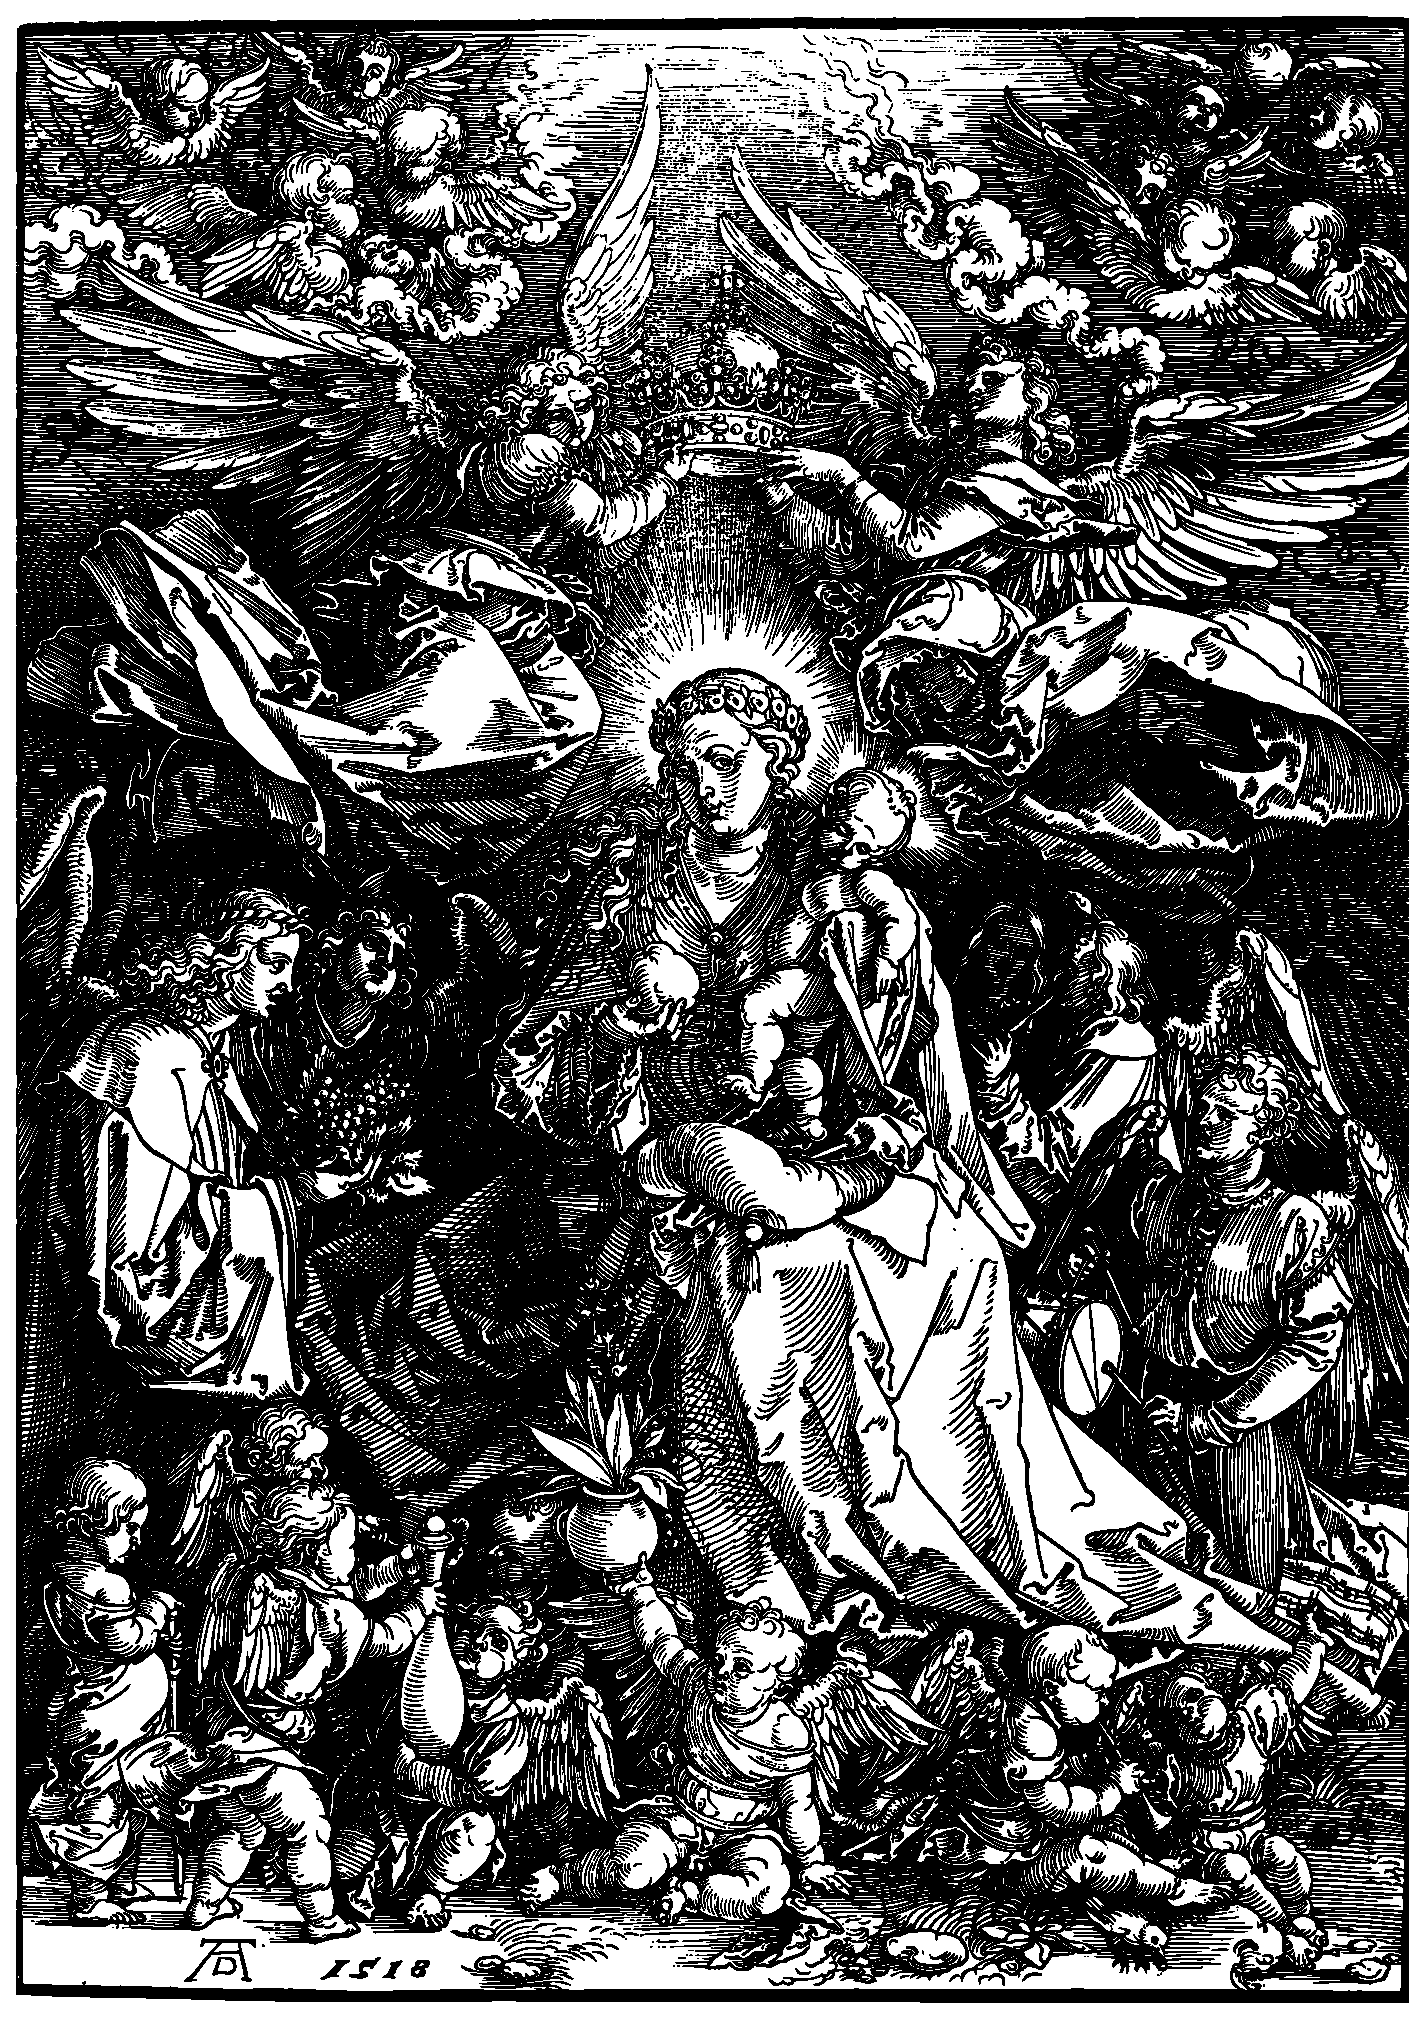
\includegraphics[width=103mm, height=146.920mm]{Lectionary/Coronation.eps}
    \caption{\textsc{\Huge{Daily Office Lectionary}}}
\end{figure}
\fancyhead[C]{{\LARGE Lectionary}}\label{lectionary}
\fancyhead[RO,LE]{\textit{Proper of Season}}
\section{Proper of Season}\label{LectionarySeason}
%Using the 1928 Lectionary is, in our opinion, the best option for a catholic American lectionary. However, it creates certain difficulties. For example, where additional proper psalms are supplied, we use them for \evensong{I}. In Advent, the same psalms are used for Mattins and \evensong{II} every Sunday, but the extra psalms are spread throughout their \evensong{I}s.

\begin{longtblr}{rowsep = 0pt,
rowhead = 1,
colspec = {p{19mm} p{19mm} p{30mm} p{26mm}},
}
Day&Psalms&Lesson 1&Lesson 2\\
\hline
	\SetCell[c=4]{l} \textsc{Advent I}\\
		\hspace{1em} Mattins&8,50&Is 55&Lk 1:57\\
		\hspace{1em} \evensong{II}&96,97&Is 60:1-11,18-end&Jn 1:15-28\\
		\SetCell[c=4]{l} \textit{Monday}\\
			\hspace{1em} Mattins&-&Gn 1:1-2:3&Mk 1:1-20\\
			\hspace{1em} \evensong{II}&-&1 Kgs 11:1-25&Rev 4\\
		\SetCell[c=4]{l} \textit{Tuesday}\\
			\hspace{1em} Mattins&-&Gn 2:4-14&Mk 1:21\\
			\hspace{1em} \evensong{II}&-&1 Kgs 11:26&Rev 5\\
		\SetCell[c=4]{l} \textit{Wednesday}\\
			\hspace{1em} Mattins&-&Gn 2:15&Mk 2\\
			\hspace{1em} \evensong{II}&-&1 Kgs 12&Rev 6\\
		\SetCell[c=4]{l} \textit{Thursday}\\
			\hspace{1em} Mattins&-&Gn 3&Mk 3\\
			\hspace{1em} \evensong{II}&-&1 Kgs 13&Rev 7\\
		\SetCell[c=4]{l} \textit{Friday}\\
			\hspace{1em} Mattins&-&Gn 4:1-15&Mk 4:1-34\\
			\hspace{1em} \evensong{II}&-&1 Kgs 14:1-20&Rev 8\\
		\SetCell[c=4]{l} \textit{Saturday}\\
			\hspace{1em} Mattins&-&Gn 4:16&Mk 4:35-5:20\\
	%1 Kgs 14:21 \& 1 Kgs 15:1-24 skipped due to Septuagesima
	\SetCell[c=4]{l} \textsc{Advent II}\\
		\hspace{1em} \evensong{I}&36,57&1 Kgs 15:25-16:7&Rev 9\\
		\hspace{1em} Mattins&80,82&Is 35&Lk 4:14-32\\
		\hspace{1em} \evensong{II}&25,26&Jdgs 16:21&Lk 6:27-42\\
		\SetCell[c=4]{l} \textit{Monday}\\
			\hspace{1em} Mattins&-&Gn 6&Mk 5:21\\
			\hspace{1em} \evensong{II}&-&1 Kgs 16:8&Rev 10\\
		\SetCell[c=4]{l} \textit{Tuesday}\\
			\hspace{1em} Mattins&-&Gn 7:1-12&Mk 6:1-29\\
			\hspace{1em} \evensong{II}&-&1 Kgs 17&Rev 11:1-18\\
		\SetCell[c=4]{l} \textit{Wednesday}\\
			\hspace{1em} Mattins&-&Gn 7:13&Mk 6:30\\
			\hspace{1em} \evensong{II}&-&1 Kgs 18&Rev 11:19-12:end\\
		%MANUAL ADJUSTMENT:
			&&&\\
			&&&\\
		\SetCell[c=4]{l} \textit{Thursday}\\
			\hspace{1em} Mattins&-&Gn 8:1-19&Mk 7\\
			\hspace{1em} \evensong{II}&-&1 Kgs 19&Rev 13\\
		\SetCell[c=4]{l} \textit{Friday}\\
			\hspace{1em} Mattins&-&Gn 8:20-9:19&Mk \\
			\hspace{1em} \evensong{II}&-&1 Kgs 20:1-25&Rev 14\\
		\SetCell[c=4]{l} \textit{Saturday}\\
			\hspace{1em} Mattins&-&Gn 9:20 \& 11:1-9&Mk 8:1-21\\
	%
	\SetCell[c=4]{l} \textsc{Advent III}\\
		\hspace{1em} \evensong{I}&96,97,98&1 Kgs 20:26&Rev 15-16\\
		\hspace{1em} Mattins&52,53&Is 40:1-11&Lk 3:1-18\\
		\hspace{1em} \evensong{II}&93,94&Is 61&Mt 9:35-10:7\\
		\SetCell[c=4]{l} \textit{Monday}\\
			\hspace{1em} Mattins&-&2 Esd 6:38-55&Mk 8:22-9:1\\
			\hspace{1em} \evensong{II}&-&1 Kgs 21&Rev 17\\
		\SetCell[c=4]{l} \textit{Tuesday}\\
			\hspace{1em} Mattins&-&Ecclus 42:15-43:10&Mk 9:2-37\\
			\hspace{1em} \evensong{II}&-&1 Kgs 22:1-28&Rev 18\\
		\SetCell[c=4]{l} \textit{Ember Wednesday}\\
			\hspace{1em} Mattins&[15,24,26]&Mal 1:1-2:7&Jn 1:29\\
			\hspace{1em} \evensong{II}&[84,132,134]&Dt 18:13&2 Tim 1:1-2:7\\
		\SetCell[c=4]{l} \textit{Thursday}\\
			\hspace{1em} Mattins&-&Ecclus 16:24-17:15&Mk 9:38-10:16\\
			\hspace{1em} \evensong{II}&-&1 Kgs 22:29&Rev 19\\
		\SetCell[c=4]{l} \textit{Ember Friday}\\
			\hspace{1em} Mattins&[15,24,26]&Mal 3:1-12&Mt 9:1-17\\
			\hspace{1em} \evensong{II}&[84,132,134]&1 Sam 3&2 Tim 2:8\\
		\SetCell[c=4]{l} \textit{Ember Saturday}\\
			\hspace{1em} Mattins&[15,24,26]&Mal 3:13-4:end&Lk 6:12-23\\
			\hspace{1em} \evensong{II}&[84,132,134]&Jer 1&2 Tim 3:14-4:8\\
	%
	\SetCell[c=4]{l} \textsc{Advent IV}\\
		\hspace{1em} Mattins&98,99&Is 52:1-10&Mt 25:1-13\\
		\hspace{1em} \evensong{II}&101,103&1 Kgs 17:1-16&Mt 3:1-12\\
		\SetCell[c=4]{l} \textit{Monday}\\
			\hspace{1em} Mattins&-&Is 1:1-20&Mk 10:17\\
			\hspace{1em} \evensong{II}&-&Dt 18:9&Rev 20-21:8\\
		%MANUAL ADJUSTMENT:
			&&&\\
			&&&\\
		\SetCell[c=4]{l} \textit{Tuesday}\\
			\hspace{1em} Mattins&-&Is 2:1-21&Mk 11\\
			\hspace{1em} \evensong{II}&-&Mic 3:5-4:7&Rev 21:9-22:end\\
		\SetCell[c=4]{l} \textit{Wednesday}\\
			\hspace{1em} Mattins&-&Is 2:22-3:15&Mk 12:1-27\\
			\hspace{1em} \evensong{II}&-&Joel 3:9&Lk 1:1-25\\
		\SetCell[c=4]{l} \textit{Thursday}\\
			\hspace{1em} Mattins&-&Is 5:1-17&Mk 12:28\\
			\hspace{1em} \evensong{II}&-&Ezek 12:21&Lk 1:26-38\\
		\SetCell[c=4]{l} \textit{Friday}\\
			\hspace{1em} Mattins&-&Is 5:18&Mk 13\\
			\hspace{1em} \evensong{II}&-&Zech 2:10&Lk 1:39-56\\
		\SetCell[c=4]{l} \textit{Saturday}\\
			\hspace{1em} Mattins&-&Is 9:8-10:4&Mt 1:18\\
	%
	\SetCell[c=4]{l} \textsc{Christmas}\\
		\hspace{1em} \evensong{I}&2,8,144&Mic 5:2-7&Lk 1:57\\
		\hspace{1em} Mattins&19,45,85&Is 9:2-7&Lk 2:1-20\\
		\hspace{1em} \evensong{II}&89:1-30,110,132&Is 7:10-16&Titus 2:11-3:7\\
	%
	%Monastic Matins: Common of a Martyr
	%1928 Lessons:
	\SetCell[c=4]{l} \textsc{St. Stephen}\\
	%Common of One Martyr Psalms:
		\hspace{1em} Mattins&64,65,92&2 Chron 24:15-25&Acts 6\\
		\hspace{1em} \evensong{II}&110,112,113,116&Wis 4:7-15&Acts 7:59-8:8\\
	%
	%Monastic Matins: Common of Apostles
	%1928 Lessons:
	\SetCell[c=4]{l} \textsc{St. John Evangelist}\\
	%Common of Apostles - Track 1 Psalms:
		\hspace{1em} Mattins&19,34,45&Ex 33:7&Jn 13:20-35\\
		\hspace{1em} \evensong{II}&116,139&Is 6:1-8&Rev 4\\
	%
	%Monastic Matins: Common of Many Martyrs
	%1928 Lessons:
	\SetCell[c=4]{l} \textsc{Holy Innocents}\\
	%Common of Many Martyrs Psalms (61 replaced with 8):
		\hspace{1em} Mattins&1,2,8,16&Jer 31:1-17&Mt 18:1-14\\
		\hspace{1em} \evensong{II}&79,110,116&2 Chron 22:8&Mk 10:13-27\\
	%
	\SetCell[c=4]{l} \textsc{Christmas I}\\
		\hspace{1em} Mattins&2,8&1 Sam 1:20&Lk 2:22-40\\
		\hspace{1em} \evensong{II}&89:1-30&Is 9:2-7&Lk 2:1-19\\
	\SetCell[c=4]{l} \textit{29 December}\\
		\hspace{1em} Mattins&-&Is 10:33-11:9&1 Jn 1:1-2:6\\
		\hspace{1em} \evensong{II}&-&Ezek 34:1-16&Lk 2:21-40\\
	\SetCell[c=4]{l} \textit{30 December}\\
		\hspace{1em} Mattins&-&Is 11:10-12:end&1 Jn 2:7-27\\
		\hspace{1em} \evensong{II}&-&Ezek 34:17&Mt 2:1-12\\
	\SetCell[c=4]{l} \textit{31 December}\\
		\hspace{1em} Mattins&-&Is 25:1-9&1 Jn 2:28-3:18\\
	%
	%1928 Psalms (expanded) \& Lessons:
	\SetCell[c=4]{l} \textsc{Circumcision}\\
		\hspace{1em} \evensong{I}&105&Dt 10:12-11:1&Mt 2:13\\
		\hspace{1em} Mattins&40,90&Ex 6:2-8&Mt 1:18\\
		\hspace{1em} \evensong{II}&65,103&Gn 32:22-30&Rev 19:11-16\\
	%
	%Monastic I Vespers: Phil 2:8-10
	%Monastic Matins: BVM Psalms ; Acts 3:1-16,4:5-12 | Lk 2:21
	\SetCell[c=4]{l} \textsc{Most Holy Name of Jesus}\\
	%AOB Psalms \& Lessons (expanded):
	\hspace{1em} Evensong&146,147&Is 7&Phil 2:1-11\\
	\hspace{1em} Mattins&9,19,24&Mic 6:1-8&Col 3:1-17\\
	\hspace{1em} \evensong{II}&110,111,112,113&Ex 34:1-10,28-end&Acts 3:1-16\\
%
	\SetCell[c=4]{l} \textsc{Christmas II}\\
		\hspace{1em} Mattins&85,87&Ex 2:1-10&Mt 2:13\\
		\hspace{1em} \evensong{II}&90,91&Prv 31:10-29&Lk 2:15-32\\
%
\SetCell[c=4]{l} \textit{3 January}\\
\hspace{1em} Mattins&-&Is 29:9-19&1 Jn 3:19-4:6\\
\hspace{1em} \evensong{II}&-&Jer 30:1-11&Jn 1:1-28\\
\SetCell[c=4]{l} \textit{4 January}\\
\hspace{1em} Mattins&-&Is 32:1-8,16-18&1 Jn 4:7\\
\hspace{1em} \evensong{II}&-&Jer 30:15-22&Jn 1:29\\
\SetCell[c=4]{l} \textit{5 January}\\
\hspace{1em} Mattins&-&Is 35&1 Jn 5\\
%
%The cycle of John readings is sped up, due to the issues regarding repetitive readings of John's literature, especially with having eight Sundays after Epiphany. Therefore, he is sped up, Hebrews is provided at the end, and the missing lessons from the insertion of Ember Days (from Mark and Luke) are provided.
\SetCell[c=4]{l} \textsc{Epiphany}\\
\hspace{1em} \evensong{I}&19,67&Num 24:15-24&Mt 28:16\\
\hspace{1em} Mattins&46,47,48&Is 60&Mt 3:13\\
\hspace{1em} \evensong{II}&72,117,135&Is 49:1-13&Jn 2:1-11\\
\SetCell[c=4]{l} \textit{Monday}\\
\hspace{1em} Mattins&-&Is 42:5-12&Gal 1\\
\hspace{1em} \evensong{II}&-&Jer 31:1-9&Jn 2:12\\
\SetCell[c=4]{l} \textit{Tuesday}\\
\hspace{1em} Mattins&-&Is 45:11-23&Gal 2\\
\hspace{1em} \evensong{II}&-&Jer 31:27-37&Jn 3:1-21\\
\SetCell[c=4]{l} \textit{Wednesday}\\
\hspace{1em} Mattins&-&Is 55&Gal 3\\
\hspace{1em} \evensong{II}&-&Jer 33:14&Jn 3:22\\
\SetCell[c=4]{l} \textit{Thursday}\\
\hspace{1em} Mattins&-&Is 56:1-8&Gal 4:1-5:1\\
\hspace{1em} \evensong{II}&-&Ezek 36:1-15&Jn 4:1-26\\
\SetCell[c=4]{l} \textit{Friday}\\
\hspace{1em} Mattins&-&Is 61&Gal 5:2\\
\hspace{1em} \evensong{II}&-&Zeph 3:7&Jn 4:27\\
\SetCell[c=4]{l} \textit{Saturday}\\
\hspace{1em} Mattins&-&Is 66:1-2,10-14,18-23&Gal 6\\
\hspace{1em} \evensong{I}&-&Zech 14:1-9&Jn 5:1-24\\
%
\SetCell[c=4]{l} \textsc{Epiphany I}\\
\hspace{1em} Mattins&47,48&Gn 28:10&Mt 2:1-11\\
\hspace{1em} \evensong{II}&66,67&1 Sam 2:1-11,26&Mt 18:1-5,10-14\\
\SetCell[c=4]{l} \textit{Monday}\\
\hspace{1em} Mattins&-&Gn 11:27-12:9&Rom 1:1-15\\
\hspace{1em} \evensong{II}&-&2 Kgs 1&Jn 5:25\\
\SetCell[c=4]{l} \textit{Tuesday}\\
\hspace{1em} Mattins&-&Gn 12:10&Rom 1:16\\
\hspace{1em} \evensong{II}&-&2 Kgs 2&Jn 6:1-21\\
\SetCell[c=4]{l} \textit{Wednesday}\\
\hspace{1em} Mattins&-&Gn 13&Rom 2:1-16\\
\hspace{1em} \evensong{II}&-&2 Kgs 3&Jn 6:22-40\\
\SetCell[c=4]{l} \textit{Thursday}\\
\hspace{1em} Mattins&-&Gn 14&Rom 2:17\\
\hspace{1em} \evensong{II}&-&2 Kgs 4:1-25a&Jn 6:41\\
\SetCell[c=4]{l} \textit{Friday}\\
\hspace{1em} Mattins&-&Gn 15&Rom 3:1-18\\
\hspace{1em} \evensong{II}&-&2 Kgs 4:25b&Jn 7:1-30\\
\SetCell[c=4]{l} \textit{Saturday}\\
\hspace{1em} Mattins&-&Gn 16&Rom 3:19\\
\hspace{1em} \evensong{I}&-&2 Kgs 5&Jn 7:31\\
%
\SetCell[c=4]{l} \textsc{Epiphany II}\\
\hspace{1em} Mattins&96,97&Ex 3:1-15&Mk 9:2-13\\
\hspace{1em} \evensong{II}&45,46&Neh 2:1-11&Acts 5:17-32\\
\SetCell[c=4]{l} \textit{Monday}\\
\hspace{1em} Mattins&-&Gn 17&Rom 4:1-13\\
\hspace{1em} \evensong{II}&-&2 Kgs 6&Jn 8:1-30\\
\SetCell[c=4]{l} \textit{Tuesday}\\
\hspace{1em} Mattins&-&Gn 18&Rom 4:14\\
\hspace{1em} \evensong{II}&-&2 Kgs 7&Jn 8:31\\
\SetCell[c=4]{l} \textit{Wednesday}\\
\hspace{1em} Mattins&-&Gn 19:1-29&Rom 5:1-11\\
\hspace{1em} \evensong{II}&-&2 Kgs 8&Jn 9:1-23\\
%MANUAL ADJUSTMENT:
&&&\\
&&&\\
\SetCell[c=4]{l} \textit{Thursday}\\
\hspace{1em} Mattins&-&Gn 19:30-20:end&Rom 5:12\\
\hspace{1em} \evensong{II}&-&2 Kgs 9&Jn 9:24\\
\SetCell[c=4]{l} \textit{Friday}\\
\hspace{1em} Mattins&-&Gn 21:1-21&Rom 6:1-14\\
\hspace{1em} \evensong{II}&-&2 Kgs 10&Jn 10:1-21\\
\SetCell[c=4]{l} \textit{Saturday}\\
\hspace{1em} Mattins&-&Gn 21:22&Rom 6:15\\
\hspace{1em} \evensong{I}&-&2 Kgs 11&Jn 10:22\\
%
\SetCell[c=4]{l} \textsc{Epiphany III}\\
\hspace{1em} Mattins&20,21&1 Sam 3:1-18&Mk 10:13-16,35-45\\
\hspace{1em} \evensong{II}&27,29&Jonah 3-4&Acts 10:1-35,44-end\\
\SetCell[c=4]{l} \textit{Monday}\\
\hspace{1em} Mattins&-&Gn 22&Rom 7:1-12\\
\hspace{1em} \evensong{II}&-&2 Kgs 12&Jn 11:1-27\\
\SetCell[c=4]{l} \textit{Tuesday}\\
\hspace{1em} Mattins&-&Gn 23&Rom 7:13\\
\hspace{1em} \evensong{II}&-&Jonah 1-2&Jn 11:28-44\\
\SetCell[c=4]{l} \textit{Wednesday}\\
\hspace{1em} Mattins&-&Gn 24:1-28&Rom 8:1-11\\
\hspace{1em} \evensong{II}&-&Jonah 3-4&Jn 11:45\\
\SetCell[c=4]{l} \textit{Thursday}\\
\hspace{1em} Mattins&-&Gn 24:29-52&Rom 8:11-25\\
\hspace{1em} \evensong{II}&-&2 Kgs 13&Jn 12:1-19\\
\SetCell[c=4]{l} \textit{Friday}\\
\hspace{1em} Mattins&-&Gn 24:53&Rom 8:26\\
\hspace{1em} \evensong{II}&-&Amos 1:1-2:3&Jn 12:20-36\\
\SetCell[c=4]{l} \textit{Saturday}\\
%\hspace{1em} Mattins&-&Gn 25:7-11,19-21,27-end&Rom 9:1-18\\
\hspace{1em} Mattins&-&Gn 25:7-11,19-end&Rom 9:1-18\\
\hspace{1em} \evensong{I}&-&Amos 2:4&Jn 12:37\\
%
\SetCell[c=4]{l} \textsc{Epiphany IV}\\
\hspace{1em} Mattins&75,76&1 Kgs 18:1,17-39&Mk 1:32\\
\hspace{1em} \evensong{II}&107&Num 22:1-35&Matt 23:16-26\\
\SetCell[c=4]{l} \textit{Monday}\\
\hspace{1em} Mattins&-&Gn 26&Rom 9:19\\
\hspace{1em} \evensong{II}&-&Amos 3-4&Jn 13:1-19\\
%MANUAL ADJUSTMENT:
&&&\\
&&&\\
\SetCell[c=4]{l} \textit{Tuesday}\\
\hspace{1em} Mattins&-&Gn 27:1-25&Rom 10:1-10\\
\hspace{1em} \evensong{II}&-&Amos 5&Jn 13:20\\
\SetCell[c=4]{l} \textit{Wednesday}\\
\hspace{1em} Mattins&-&Gn 27:26-45&Rom 10:11\\
\hspace{1em} \evensong{II}&-&Amos 6&Jn 14\\
\SetCell[c=4]{l} \textit{Thursday}\\
\hspace{1em} Mattins&-&Gn 27:46-28:end&Rom 11:1-11\\
\hspace{1em} \evensong{II}&-&Amos 7&Jn 15\\
\SetCell[c=4]{l} \textit{Friday}\\
\hspace{1em} Mattins&-&Gn 29:1-20&Rom 11:12-24\\
\hspace{1em} \evensong{II}&-&Amos 8&Jn 16\\
\SetCell[c=4]{l} \textit{Saturday}\\
\hspace{1em} Mattins&-&Gn 29:21&Rom 11:25\\
\hspace{1em} \evensong{I}&-&Amos 9&Jn 17\\
%
\SetCell[c=4]{l} \textsc{Epiphany V}\\
\hspace{1em} Mattins&63,65&1 Kgs 18:41-19:end&Mk 8:22-9:1\\
\hspace{1em} \evensong{II}&78&Num 23:1-26&Acts 5:1-11\\
\SetCell[c=4]{l} \textit{Monday}\\
%Correcting error in 1928 Lectionary (skips a verse):
\hspace{1em} Mattins&-&Gn 30:1-24&Rom 12\\
\hspace{1em} \evensong{II}&-&Hos 4&Jn 18:1-27\\
\SetCell[c=4]{l} \textit{Tuesday}\\
\hspace{1em} Mattins&-&Gn 30:25-31:3&Rom 13\\
\hspace{1em} \evensong{II}&-&Hos 5-6&Jn 18:28-19:16\\
\SetCell[c=4]{l} \textit{Wednesday}\\
\hspace{1em} Mattins&-&Gn 31:4-24&Rom 14:1-18\\
\hspace{1em} \evensong{II}&-&Hos 10&Jn 19:17\\
\SetCell[c=4]{l} \textit{Thursday}\\
\hspace{1em} Mattins&-&Gn 31:25&Rom 14:19-15:12\\
\hspace{1em} \evensong{II}&-&Hos 11&Jn 20:1-18\\
\SetCell[c=4]{l} \textit{Friday}\\
\hspace{1em} Mattins&-&Gn 32&Rom 15:13\\
\hspace{1em} \evensong{II}&-&Hos 13-14&Jn 20:19\\
\SetCell[c=4]{l} \textit{Saturday}\\
\hspace{1em} Mattins&-&Gn 33&Rom 16\\
\hspace{1em} \evensong{I}&-&2 Kgs 14&Jn 21\\
%
%MANUAL ADJUSTMENT:
&&&\\
&&&\\
\SetCell[c=4]{l} \textsc{Epiphany VI}\\
\hspace{1em} Mattins&146,147&Dan 3:8&Mk 10:46\\
\hspace{1em} \evensong{II}&148,149,150&Num 24:2&Lk 10:1-16\\
\SetCell[c=4]{l} \textit{Monday}\\
\hspace{1em} Mattins&-&Wis 1:1-14,2:23-end&2 Pet 1\\
\hspace{1em} \evensong{II}&-&2 Kgs 15&Heb 1\\
\SetCell[c=4]{l} \textit{Tuesday}\\
\hspace{1em} Mattins&-&Wis 4:7-15&2 Pet 2\\
\hspace{1em} \evensong{II}&-&2 Kgs 17:1-23&Heb 2\\
\SetCell[c=4]{l} \textit{Wednesday}\\
\hspace{1em} Mattins&-&Wis 6:1-21&2 Pet 3\\
\hspace{1em} \evensong{II}&-&2 Kgs 17:24&Heb 3\\
\SetCell[c=4]{l} \textit{Thursday}\\
\hspace{1em} Mattins&-&Wis 6:22-7:14&Jude\\
\hspace{1em} \evensong{II}&-&Nah 1&Heb 3\\
\SetCell[c=4]{l} \textit{Friday}\\
\hspace{1em} Mattins&-&Wis 8:1-18&2 Jn\\
\hspace{1em} \evensong{II}&-&Nah 2&Heb 4\\
\SetCell[c=4]{l} \textit{Saturday}\\
\hspace{1em} Mattins&-&Wis 9:1-16&3 Jn\\
\hspace{1em} \evensong{I}&-&Nah 3&Heb 5\\
%Taken from Trinity XXV:
\SetCell[c=4]{l} \textsc{Epiphany VII}\\
%1962 Lectionary Lessons (Year I) from Trinity XXV used for Sunday lessons.
\hspace{1em} Mattins&75,76&2 Esd 16:53-67&Jas 4\\
\hspace{1em} \evensong{II}&107&Bar 3:1-14&Mt 21:33\\
\SetCell[c=4]{l} \textit{Monday}\\
\hspace{1em} Mattins&-&Prv 22:17&Mk 9:2-29\\
\hspace{1em} \evensong{II}&-&Ecclus 28&Heb 6\\
\SetCell[c=4]{l} \textit{Tuesday}\\
\hspace{1em} Mattins&-&Prv 23:19&Mk 9:30\\
\hspace{1em} \evensong{II}&-&Ecclus 29&Heb 7:1-17\\
\SetCell[c=4]{l} \textit{Wednesday}\\
\hspace{1em} Mattins&-&Prv 24:1-22&Mk 10:1-31\\
\hspace{1em} \evensong{II}&-&Ecclus 35&Heb 7:18\\
\SetCell[c=4]{l} \textit{Thursday}\\
\hspace{1em} Mattins&-&Prv 24:23&Mk 10:32\\
\hspace{1em} \evensong{II}&-&Eccles 1&Heb 8\\
%MANUAL ADJUSTMENT:
&&&\\
&&&\\
\SetCell[c=4]{l} \textit{Friday}\\
\hspace{1em} Mattins&-&Prv 25&Acts 8:14\\
\hspace{1em} \evensong{II}&-&Eccles 2&Heb 9:1-10\\
\SetCell[c=4]{l} \textit{Saturday}\\
\hspace{1em} Mattins&-&Prv 26&Acts 9:1-22\\
\hspace{1em} \evensong{I}&-&Eccles 3&Heb 9:11\\
%Taken from Trinity XXVI:
\SetCell[c=4]{l} \textsc{Epiphany VIII}\\
%1962 Lectionary Lessons (Year I) from Trinity XXVI used for Sunday lessons.
\hspace{1em} Mattins&63,65&Prayer of Manasses&Jas 5\\
\hspace{1em} \evensong{II}&78&Bar 4:36-5:end&Mt 23:1-22\\
\SetCell[c=4]{l} \textit{Monday}\\
\hspace{1em} Mattins&-&Prv 27&Acts 13:33\\
\hspace{1em} \evensong{II}&-&Eccles 5&Heb 10:1-18\\
\SetCell[c=4]{l} \textit{Tuesday}\\
\hspace{1em} Mattins&-&Prv 28&Acts 14\\
\hspace{1em} \evensong{II}&-&Eccles 6:1-7:8&Heb 10:19\\
\SetCell[c=4]{l} \textit{Wednesday}\\
\hspace{1em} Mattins&-&Prv 29&Rev 17\\
\hspace{1em} \evensong{II}&-&Eccles 8:1-15&Heb 11:1-16\\
\SetCell[c=4]{l} \textit{Thursday}\\
\hspace{1em} Mattins&-&Prv 30:1-16&Rev 18\\
\hspace{1em} \evensong{II}&-&Eccles 8:16-9:end&Heb 11:17\\
\SetCell[c=4]{l} \textit{Friday}\\
\hspace{1em} Mattins&-&Prv 30:17&Rev 19\\
\hspace{1em} \evensong{II}&-&Eccles 10&Heb 12\\
\SetCell[c=4]{l} \textit{Saturday}\\
\hspace{1em} Mattins&-&Prv 31&Rev 20\\
\hspace{1em} \evensong{I}&-&Eccles 11-12&Heb 13\\
%
\SetCell[c=4]{l} \textsc{Septuagesima}\\
\hspace{1em} Mattins&8,148&Josh 6:1-21&Lk 7:1-10\\
\hspace{1em} \evensong{II}&104&Lam 1:1-12&Mt 23:29-24:2\\
\SetCell[c=4]{l} \textit{Monday}\\
\hspace{1em} Mattins&-&Gn 34&Phil 1:1-11\\
\hspace{1em} \evensong{II}&-&1 Kgs 14:21&Mt 5:1-20\\
\SetCell[c=4]{l} \textit{Tuesday}\\
\hspace{1em} Mattins&-&Gn 35-36:8&Phil 1:12\\
\hspace{1em} \evensong{II}&-&1 Kgs 15:1-24&Mt 5:21\\
%MANUAL ADJUSTMENT:
&&&\\
&&&\\
\SetCell[c=4]{l} \textit{Wednesday}\\
\hspace{1em} Mattins&-&Gn 37&Phil 2:1-13\\
%CHECK:
\hspace{1em} \evensong{II}&\SetCell[c=2]{l} - \hspace{3em} 2 Chron 19:4-end,20:30-end&&Mt 6:1-18\\
\SetCell[c=4]{l} \textit{Thursday}\\
\hspace{1em} Mattins&-&Gn 38&Phil 2:14\\
\hspace{1em} \evensong{II}&-&2 Chron 21&Mt 6:19\\
\SetCell[c=4]{l} \textit{Friday}\\
\hspace{1em} Mattins&-&Gn 39&Phil 3\\
\hspace{1em} \evensong{II}&-&2 Chron 22&Mt 7:1-27\\
\SetCell[c=4]{l} \textit{Saturday}\\
\hspace{1em} Mattins&-&Gn 40&Phil 4\\
\hspace{1em} \evensong{I}&-&2 Chron 23&Mt 13:24-52\\
%
\SetCell[c=4]{l} \textsc{Sexagesima}\\
\hspace{1em} Mattins&33,93&1 Sam 17:17&Mt 10:32-39\\
\hspace{1em} \evensong{II}&139&2 Sam 22:1-12,33-36&Acts 12:1-17\\
\SetCell[c=4]{l} \textit{Monday}\\
\hspace{1em} Mattins&-&Gn 41:1-36&Jas 1:1-15\\
\hspace{1em} \evensong{II}&-&2 Chron 24&Mt 15:1-20\\
\SetCell[c=4]{l} \textit{Tuesday}\\
\hspace{1em} Mattins&-&Gn 41:37&Jas 1:16\\
\hspace{1em} \evensong{II}&-&2 Chron 25&Mt 18:1-14\\
\SetCell[c=4]{l} \textit{Wednesday}\\
\hspace{1em} Mattins&-&Gn 42:1-17&Jas 2:1-13\\
\hspace{1em} \evensong{II}&-&2 Chron 26-27&Mt 18:15\\
\SetCell[c=4]{l} \textit{Thursday}\\
\hspace{1em} Mattins&-&Gn 42:18&Jas 2:14\\
\hspace{1em} \evensong{II}&-&2 Kgs 16&Mt 20:1-16\\
\SetCell[c=4]{l} \textit{Friday}\\
\hspace{1em} Mattins&-&Gn 43:1-14&Jas 3:1-13\\
\hspace{1em} \evensong{II}&-&2 Chron 30&Mt 22:1-14\\
\SetCell[c=4]{l} \textit{Saturday}\\
\hspace{1em} Mattins&-&Gn 43:15&Jas 3:13-4:6\\
\hspace{1em} \evensong{I}&-&2 Chron 32:1-23&Mt 25:1-13\\
%
\SetCell[c=4]{l} \textsc{Quinquagesima}\\
\hspace{1em} Mattins&15,16&Ruth 1:1-17&Jn 15:1-17\\
\hspace{1em} \evensong{II}&111,112&Is 63:7-9,14-16&1 Jn 4\\
%MANUAL ADJUSTMENT:
&&&\\
&&&\\
\SetCell[c=4]{l} \textit{Monday}\\
\hspace{1em} Mattins&-&Gn 44&Jas 4:7\\
\hspace{1em} \evensong{II}&-&2 Kgs 20&Mt 25:14-30\\
\SetCell[c=4]{l} \textit{Tuesday}\\
\hspace{1em} Mattins&-&Gn 45:1-15&Jas 5\\
\hspace{1em} \evensong{II}&-&Mic 6&Mt 25:31\\
%
\SetCell[c=4]{l} \textsc{Ash Wednesday}\\
\hspace{1em} Mattins&6,32,38&Is 58&Lk 15\\
\hspace{1em} \evensong{II}&102,130,143&Is 1:2-20&Lk 3:1-22\\
\SetCell[c=4]{l} \textit{Thursday}\\
\hspace{1em} Mattins&-&Gn 45:16&1 Cor 1\\
\hspace{1em} \evensong{II}&-&2 Chron 33&Lk 4:1-29\\
\SetCell[c=4]{l} \textit{Friday}\\
\hspace{1em} Mattins&-&Gn 46:1-7,26-end&1 Cor 2-3\\
\hspace{1em} \evensong{II}&-&2 Kgs 22:1-23:3&Lk 4:30-5:16\\
\SetCell[c=4]{l} \textit{Saturday}\\
\hspace{1em} Mattins&-&Gn 47&1 Cor 4\\
\hspace{1em} \evensong{I}&-&2 Kgs 23:4-35&Lk 5:17\\
%
\SetCell[c=4]{l} \textsc{Lent I}\\
\hspace{1em} Mattins&51,54&2 Sam 11:1-12:14&Lk 18:10-14\\
\hspace{1em} \evensong{II}&119:1-32&1 Sam 26:5&Mk 1:9-28\\
\SetCell[c=4]{l} \textit{Monday}\\
\hspace{1em} Mattins&-&Gn 48&1 Cor 5-6:11\\
\hspace{1em} \evensong{II}&-&Hab 1:1-2:4&Lk 6:1-26\\
\SetCell[c=4]{l} \textit{Tuesday}\\
\hspace{1em} Mattins&-&Gn 49&1 Cor 6:12-7:16\\
\hspace{1em} \evensong{II}&-&Jer 13&Lk 6:27\\
\SetCell[c=4]{l} \textit{Ember Wednesday}\\
\hspace{1em} Mattins&[15,24,26]&1 Sam 2:27-35&Lk 10:1-24\\
\hspace{1em} \evensong{II}&[84,132,134]&Jer 26&2 Cor 3\\
\SetCell[c=4]{l} \textit{Thursday}\\
\hspace{1em} Mattins&-&Gn 50&1 Cor 7:17\\
\hspace{1em} \evensong{II}&-&Jer 36&Lk 7:1-23\\
\SetCell[c=4]{l} \textit{Ember Friday}\\
\hspace{1em} Mattins&[15,24,26]&Ezek 33:1-20&Mt 10:1-23\\
\hspace{1em} \evensong{II}&[84,132,134]&Amos 7:1-15&2 Cor 4:1-5:4\\
%MANUAL ADJUSTMENT:
&&&\\
&&&\\
\SetCell[c=4]{l} \textit{Ember Saturday}\\
\hspace{1em} Mattins&[15,24,26]&Ezek 44:4-16,23-24&Mt 10:24\\
\hspace{1em} \evensong{II}&[84,132,134]&Neh 8:1-12&2 Cor 5:5-6:10\\
%
\SetCell[c=4]{l} \textsc{Lent II}\\
\hspace{1em} Mattins&6,38&1 Kgs 21:1-20&Mk 10:17-31\\
\hspace{1em} \evensong{II}&119:33-72&1 Sam 19:1-18&Mt 21:33\\
\SetCell[c=4]{l} \textit{Monday}\\
\hspace{1em} Mattins&-&Wis 9:17-10:14&1 Cor 8-9:23\\
\hspace{1em} \evensong{II}&-&2 Kgs 23:36-24:17&Lk 7:24\\
\SetCell[c=4]{l} \textit{Tuesday}\\
\hspace{1em} Mattins&-&Ex 1&1 Cor 9:24-10:22\\
\hspace{1em} \evensong{II}&-&Jer 24&Lk 8:1-25\\
\SetCell[c=4]{l} \textit{Wednesday}\\
\hspace{1em} Mattins&-&Ex 2&1 Cor 10:23-11:16\\
\hspace{1em} \evensong{II}&-&Jer 29:1-14&Lk 8:26\\
\SetCell[c=4]{l} \textit{Thursday}\\
\hspace{1em} Mattins&-&Ex 3&1 Cor 11:17\\
\hspace{1em} \evensong{II}&-&Jer 21&Lk 9:1-17\\
\SetCell[c=4]{l} \textit{Friday}\\
\hspace{1em} Mattins&-&Ex 4:1-26&1 Cor 12:1-26\\
\hspace{1em} \evensong{II}&-&Jer 18&Lk 9:18-36\\
\SetCell[c=4]{l} \textit{Saturday}\\
\hspace{1em} Mattins&-&Ex 4:27-5:21&1 Cor 12:27-13:end\\
\hspace{1em} \evensong{I}&-&Jer 19:1-20:6&Lk 9:37\\
%
\SetCell[c=4]{l} \textsc{Lent III}\\
\hspace{1em} Mattins&56,86&Gn 50:7-21&Mt 18:21\\
\hspace{1em} \evensong{II}&119:73-104&Gn 27:1-38&Mt 20:1-28\\
\SetCell[c=4]{l} \textit{Monday}\\
\hspace{1em} Mattins&-&Ex 5:22-6:13&1 Cor 14:1-19\\
\hspace{1em} \evensong{II}&-&Jer 27&Lk 10:1-24\\
\SetCell[c=4]{l} \textit{Tuesday}\\
\hspace{1em} Mattins&-&Ex 6:28-7:25&1 Cor 14:20\\
\hspace{1em} \evensong{II}&-&Jer 28&Lk 10:25\\
\SetCell[c=4]{l} \textit{Wednesday}\\
\hspace{1em} Mattins&-&Ex 8:1-19&1 Cor 15:1-22\\
\hspace{1em} \evensong{II}&-&Jer 34&Lk 11:1-28\\
%MANUAL ADJUSTMENT:
&&&\\
&&&\\
\SetCell[c=4]{l} \textit{Thursday}\\
\hspace{1em} Mattins&-&Ex 8:20&1 Cor 15:20-34\\
\hspace{1em} \evensong{II}&-&Jer 35&Lk 11:29\\
\SetCell[c=4]{l} \textit{Friday}\\
\hspace{1em} Mattins&-&Ex 9:1-12&1 Cor 15:35\\
\hspace{1em} \evensong{II}&-&Jer 37&Lk 12:1-12\\
\SetCell[c=4]{l} \textit{Saturday}\\
\hspace{1em} Mattins&-&Ex 9:13&1 Cor 16\\
\hspace{1em} \evensong{I}&-&Jer 38&Lk 12:13-34\\
%
\SetCell[c=4]{l} \textsc{Lent IV}\\
\hspace{1em} Mattins&142,143&2 Sam 18:5&Lk 15:11\\
\hspace{1em} \evensong{II}&119:105-144&Gn 13&Mt 7:13\\
\SetCell[c=4]{l} \textit{Monday}\\
\hspace{1em} Mattins&-&Ex 10:1-20&2 Cor 1:1-22\\
\hspace{1em} \evensong{II}&-&2 Kgs 24:18-25:11,20-22&Lk 12:35\\
\SetCell[c=4]{l} \textit{Tuesday}\\
\hspace{1em} Mattins&-&Ex 10:21-11:10&2 Cor 1:23-2:end\\
\hspace{1em} \evensong{II}&-&Jer 39:11-40:end&Lk 13:1-17\\
\SetCell[c=4]{l} \textit{Wednesday}\\
\hspace{1em} Mattins&-&Ex 12:1-28&2 Cor 3:1-4:6\\
\hspace{1em} \evensong{II}&-&Jer 41&Lk 13:18\\
\SetCell[c=4]{l} \textit{Thursday}\\
\hspace{1em} Mattins&-&Ex 12:29&2 Cor 4:7-5:10\\
\hspace{1em} \evensong{II}&-&Jer 42&Lk 14:1-24\\
\SetCell[c=4]{l} \textit{Friday}\\
\hspace{1em} Mattins&-&Ex 13&2 Cor 5:11-6:10\\
\hspace{1em} \evensong{II}&-&Jer 43&Lk 14:25\\
\SetCell[c=4]{l} \textit{Saturday}\\
\hspace{1em} Mattins&-&Ex 14&2 Cor 6:11-7:end\\
\hspace{1em} \evensong{I}&-&Jer 44&Lk 15\\
%
\SetCell[c=4]{l} \textsc{Passion Sunday}\\
\hspace{1em} Mattins&42,43&Gn 22:1-13&Jn 10:1-16\\
\hspace{1em} \evensong{II}&119:145-176&1 Kgs 8:22-53&Jn 17\\
\SetCell[c=4]{l} \textit{Passion Monday}\\
\hspace{1em} Mattins&-&Wis 10:15-11:4&2 Cor 8:1-22\\
\hspace{1em} \evensong{II}&-&Dan 1&Lk 16:1-18\\
%MANUAL ADJUSTMENT:
&&&\\
&&&\\
\SetCell[c=4]{l} \textit{Passion Tuesday}\\
\hspace{1em} Mattins&-&Ex 15:1-21&2 Cor 8:23-9:end\\
\hspace{1em} \evensong{II}&-&Dan 3&Lk 16:19-17:10\\
\SetCell[c=4]{l} \textit{Passion Wednesday}\\
\hspace{1em} Mattins&-&Ex 15:22-16:10&2 Cor 10\\
\hspace{1em} \evensong{II}&-&Dan 4&Lk 17:11\\
\SetCell[c=4]{l} \textit{Passion Thursday}\\
\hspace{1em} Mattins&-&Ex 16:11&2 Cor 11\\
\hspace{1em} \evensong{II}&-&Dan 5&Lk 18:1-17\\
\SetCell[c=4]{l} \textit{Passion Friday}\\
\hspace{1em} Mattins&-&Ex 17&2 Cor 12\\
\hspace{1em} \evensong{II}&-&Dan 6&Lk 18:18\\
\SetCell[c=4]{l} \textit{Passion Saturday}\\
\hspace{1em} Mattins&-&Ex 18&2 Cor 13\\
\hspace{1em} \evensong{I}&-&Dan 9&Lk 19:1-28\\
\SetCell[c=4]{l} \textsc{Palm Sunday}\\
\hspace{1em} Mattins&97,110&Zech 9:9-16&Mk 11:1-11\\
\hspace{1em} \evensong{II}&22,23&Is 52:13-53:end&Lk 19:28b-44\\
%Too much permission is given for the Holy Week psalms, so I follow the 1929 Scottish Prayer Book.
\SetCell[c=4]{l} \textit{Holy Monday}\\
\hspace{1em} Mattins&6,32,38&Num 20:1-13&1 Cor 10:1-13\\
\hspace{1em} \evensong{II}&42,43&Is 5:1-7&Lk 19:45-20:26\\
\SetCell[c=4]{l} \textit{Holy Tuesday}\\
\hspace{1em} Mattins&51,55&Num 21:1-9&Jn 3:1-21\\
\hspace{1em} \evensong{II}&102,130&Is 2:2-5&Lk 20:27-21:19\\
\SetCell[c=4]{l} \textit{Spy Wednesday}\\
\hspace{1em} Mattins&138,139&Is 42:1-12&Jn 10:11-18\\
\hspace{1em} \evensong{II}&140,141&Gn 37:3-28&Lk 21:20-22:6\\
\SetCell[c=4]{l} \textit{Maundy Thursday}\\
\hspace{1em} Mattins&81,116&Jer 31:31-34&Jn 13:1-17,33-35\\
\hspace{1em} \evensong{II}&142,143&Ex 16:4-15&Lk 22:7-23,39-54\\
%
\SetCell[c=4]{l} \textit{Good Friday}\\
\hspace{1em} Mattins&22:1-19,40:1-16,54&Gn 22:1-18&Jn 18\\
\hspace{1em} \evensong{II}&64,69:1-22,88&Is 52:13-53:end&Lk 23:13-47\\
\SetCell[c=4]{l} \textit{Easter Even}\\
\hspace{1em} Mattins&4,16,17&Job 14:1-15&Rom 6:3-11\\
%
%MANUAL ADJUSTMENT:
&&&\\
&&&\\
\SetCell[c=4]{l} \textsc{Easter Day}\\
\hspace{1em} \evensong{I}&27,30,31&Ex 12:1-14&Lk 23:50\\
\hspace{1em} Mattins&2,57,111&Is 51:9-16&Lk 24:1-12\\
\hspace{1em} \evensong{II}&113,114,118&Ex 15:1-21&Mt 28:1-10,16-end\\
\SetCell[c=4]{l} \textit{Easter Monday}\\
\hspace{1em} Mattins&-&Ex 19:1-15&Mk 16:1-8\\
\hspace{1em} \evensong{II}&-&Is 40&Lk 24:13-35\\
\SetCell[c=4]{l} \textit{Easter Tuesday}\\
\hspace{1em} Mattins&-&Ex 19:16-20:26&Jn 20:1-18\\
\hspace{1em} \evensong{II}&-&Is 41&Lk 24:36-49\\
\SetCell[c=4]{l} \textit{Easter Wednesday}\\
\hspace{1em} Mattins&-&Ex 21:1-32&Mk 8:27-9:1\\
\hspace{1em} \evensong{II}&-&Is 42&Jn 20:19\\
\SetCell[c=4]{l} \textit{Easter Thursday}\\
\hspace{1em} Mattins&-&Ex 21:33-22:31&Mk 9:2-13,30-32\\
\hspace{1em} \evensong{II}&-&Is 43&Jn 21:1-14\\
\SetCell[c=4]{l} \textit{Easter Friday}\\
\hspace{1em} Mattins&-&Ex 23&Mk 10:32-45\\
\hspace{1em} \evensong{II}&-&Is 44&Jn 21:15\\
\SetCell[c=4]{l} \textit{Easter Saturday}\\
\hspace{1em} Mattins&-&Ex 24&Mk 14:17,22-28\\
\hspace{1em} \evensong{I}&-&Is 45&Mk 16:9\\
%
\SetCell[c=4]{l} \textsc{Easter I}\\
\hspace{1em} Mattins&110,111&2 Kgs 4:18-37&Lk 24:13-35\\
\hspace{1em} \evensong{II}&2,57&Job 19:1,13-27a&Jn 14:1-14\\
\SetCell[c=4]{l} \textit{Monday}\\
\hspace{1em} Mattins&-&Ex 25:1-22&1 Pet 1:1-21\\
\hspace{1em} \evensong{II}&-&Is 46&Mk 5:22\\
\SetCell[c=4]{l} \textit{Tuesday}\\
\hspace{1em} Mattins&-&Ex 25:23&1 Pet 1:22-2:10\\
\hspace{1em} \evensong{II}&-&Is 47&Lk 7:11-16\\
\SetCell[c=4]{l} \textit{Wednesday}\\
\hspace{1em} Mattins&-&Ex 31&1 Pet 2:11\\
\hspace{1em} \evensong{II}&-&Is 48&Jn 11:1-44\\
\SetCell[c=4]{l} \textit{Thursday}\\
\hspace{1em} Mattins&-&Ex 32:1-24&1 Pet 3\\
\hspace{1em} \evensong{II}&-&Is 49&Jn 5:19-30\\
%MANUAL ADJUSTMENT:
&&&\\
\SetCell[c=4]{l} \textit{Friday}\\
\hspace{1em} Mattins&-&Ex 32:25-33:23&1 Pet 4\\
\hspace{1em} \evensong{II}&-&Is 50&Jn 6:25-58\\
\SetCell[c=4]{l} \textit{Saturday}\\
\hspace{1em} Mattins&-&Ex 34:1-14,27-35&1 Pet 5\\
\hspace{1em} \evensong{I}&-&Is 51&Mk 13:18-27\\
%
\SetCell[c=4]{l} \textsc{Easter II}\\
\hspace{1em} Mattins&21,23&2 Sam 1:19&Jn 20:24\\
\hspace{1em} \evensong{II}&116,117&Ezek 34:11-16,30-31&Jn 10:1-11\\
\SetCell[c=4]{l} \textit{Monday}\\
\hspace{1em} Mattins&-&Ex 35:20-36:1&Col 1\\
\hspace{1em} \evensong{II}&-&Is 52&Acts 3:12\\
\SetCell[c=4]{l} \textit{Tuesday}\\
\hspace{1em} Mattins&-&Ex 40:17&Col 2\\
%
%Monastic I Vespers: Common of Apostles Psalms ; Gen 49:26
%Monastic Matins: Common of Confessor Bishop Psalms ; Gen 39:1-6,41:37-49 | | Luke 3:21-23
\SetCell[c=4]{l} \textsc{Patronage of St. Joseph}\\
%Eastertide readings skipped, consolidated with the surrounding readings, if possible.
%AOB Psalms \& Lessons for 19 March
\hspace{1em} \evensong{I}&110,117,146&Gn 39&Mt 1:18\\
\hspace{1em} Mattins&1,2,3&Gn 41:38&Mt 2:13\\
\hspace{1em} \evensong{II}&112,116,126&Gn 49:22-26&Lk 2:41\\
%
\SetCell[c=4]{l} \textit{Thursday}\\
\hspace{1em} Mattins&-&Num 9&Col 3\\
\hspace{1em} \evensong{II}&-&Is 53&Acts 17:22-31\\
\SetCell[c=4]{l} \textit{Friday}\\
\hspace{1em} Mattins&-&Num 10:1-13,29-end&Col 4\\
\hspace{1em} \evensong{II}&-&Is 54&Acts 26:1-23\\
\SetCell[c=4]{l} \textit{Saturday}\\
\hspace{1em} Mattins&-&Num 11:1-30&Philemon\\
\hspace{1em} \evensong{I}&-&Is 55&Acts 9:32\\
%
\SetCell[c=4]{l} \textsc{Easter III}\\
\hspace{1em} Mattins&120,121,122&2 Sam 12:15b-23&Jn 21:1-19\\
\hspace{1em} \evensong{II}&123,124,125&Ex 14:5&Rom 6:1-18\\
\SetCell[c=4]{l} \textit{Monday}\\
\hspace{1em} Mattins&-&Num 11:31-12:16&Eph 1\\
\hspace{1em} \evensong{II}&-&Is 56&1 Cor 15:1-28\\
\SetCell[c=4]{l} \textit{Tuesday}\\
\hspace{1em} Mattins&-&Num 13:1-3,17-25&Eph 2\\
\hspace{1em} \evensong{II}&-&Is 57&1 Cor 15:29\\
%MANUAL ADJUSTMENT:
&&&\\
&&&\\
\SetCell[c=4]{l} \textit{Wednesday}\\
\hspace{1em} Mattins&-&Num 13:26-14:10&Eph 3\\
\hspace{1em} \evensong{II}&-&Is 58&2 Cor 5:5\\
\SetCell[c=4]{l} \textit{Thursday}\\
\hspace{1em} Mattins&-&Num 14:11-25&Eph 4:1-16\\
\hspace{1em} \evensong{II}&-&Is 59&Rom 1:1-12\\
\SetCell[c=4]{l} \textit{Friday}\\
\hspace{1em} Mattins&-&Num 14:26&Eph 4:17\\
\hspace{1em} \evensong{II}&-&Is 60&Rom 6:1-13\\
\SetCell[c=4]{l} \textit{Saturday}\\
\hspace{1em} Mattins&-&Num 16:1-40&Eph 5:1-21\\
\hspace{1em} \evensong{I}&-&Is 61&Rom 14:1-9\\
%
\SetCell[c=4]{l} \textsc{Easter IV}\\
\hspace{1em} Mattins&126,127,128&2 Esd 2:42-47&Jn 11:17-39a,41-44\\
\hspace{1em} \evensong{II}&129,130,131&Gn 8:6-12,15-16,9:8-16&Mk 12:18-27a\\
\SetCell[c=4]{l} \textit{Monday}\\
\hspace{1em} Mattins&-&Num 16:41-17:11&Eph 5:22-6:9\\
\hspace{1em} \evensong{II}&-&Is 62&Phil 3:7\\
\SetCell[c=4]{l} \textit{Tuesday}\\
\hspace{1em} Mattins&-&Num 17:12-18:24&Eph 6:10\\
\hspace{1em} \evensong{II}&-&Is 63&2 Cor 1:1-10\\
\SetCell[c=4]{l} \textit{Wednesday}\\
\hspace{1em} Mattins&-&Num 20:1-21&Heb 1:1-12\\
\hspace{1em} \evensong{II}&-&Is 64&2 Cor 4:6-5:1\\
\SetCell[c=4]{l} \textit{Thursday}\\
\hspace{1em} Mattins&-&Num 20:22-21:9&Heb 1:13-2:13\\
\hspace{1em} \evensong{II}&-&Is 65:1-12&Rom 8:1-17\\
\SetCell[c=4]{l} \textit{Friday}\\
\hspace{1em} Mattins&-&Num 21:10-35&Heb 2:14-3:end\\
\hspace{1em} \evensong{II}&-&Is 65:13&1 Cor 15:35\\
\SetCell[c=4]{l} \textit{Saturday}\\
\hspace{1em} Mattins&-&Num 22:1-14&Heb 4:1-13\\
\hspace{1em} \evensong{I}&-&Is 66&Rev 21:1-7\\
%
\SetCell[c=4]{l} \textsc{Rogation Sunday}\\
\hspace{1em} Mattins&146,147&Ezek 37:1-14&Lk 24:36-49\\
\hspace{1em} \evensong{II}&132,133,134&Job 14:1-15&Mt 19:16-29\\
%MANUAL ADJUSTMENT:
&&&\\
&&&\\
\SetCell[c=4]{l} \textit{Rogation Monday}\\
\hspace{1em} Mattins&-&Dt 28:1-14&Mt 6:24\\
\hspace{1em} \evensong{II}&-&Dt 8&Jas 1:1-17\\
\SetCell[c=4]{l} \textit{Rogation Tuesday}\\
\hspace{1em} Mattins&-&Is 64&Lk 11:1-13\\
\hspace{1em} \evensong{II}&-&1 Kgs 8:22-40&Jas 4\\
\SetCell[c=4]{l} \textit{Ascension Even}\\
\hspace{1em} Mattins&-&Jer 14&Jn 6:27-63\\
%
\SetCell[c=4]{l} \textsc{Ascension Thursday}\\
\hspace{1em} \evensong{I}&93,99&Gn 5:18-24&Eph 4:1-13\\
\hspace{1em} Mattins&8,15,21&2 Kgs 2:1-15&Heb 4:14-5:10\\
\hspace{1em} \evensong{II}&24,47,108:1-6&Dan 7:9-14&Lk 24:44\\
\SetCell[c=4]{l} \textit{Friday}\\
\hspace{1em} Mattins&-&Num 22:15-35&Heb 5:11-6:end\\
\hspace{1em} \evensong{II}&-&Obadiah&1 Pet 3:8\\
\SetCell[c=4]{l} \textit{Saturday}\\
\hspace{1em} Mattins&-&Num 22:36-23:26&Heb 7\\
\hspace{1em} \evensong{I}&-&Hab 1&Phil 2:1-11\\
%
\SetCell[c=4]{l} \textsc{Sunday within Ascension Octave}\\
\hspace{1em} Mattins&108,110&2 Kgs 2:1-22&Acts 1\\
\hspace{1em} \evensong{II}&46,47&Dt 34&Jn 14:15-27\\
\SetCell[c=4]{l} \textit{Monday}\\
\hspace{1em} Mattins&-&Num 23:27-24:25&Heb 8:1-9:12\\
\hspace{1em} \evensong{II}&-&Hab 2&Jn 14:1-14\\
\SetCell[c=4]{l} \textit{Tuesday}\\
\hspace{1em} Mattins&-&Num 25&Heb 9:11\\
\hspace{1em} \evensong{II}&-&Hab 3&Jn 14:15\\
\SetCell[c=4]{l} \textit{Wednesday}\\
%CHECK:
\hspace{1em} Mattins&\SetCell[c=2]{l} - \hspace{3em} Num 26:1-4,52-56,63-end; 27:12&&Heb 10:1-34\\
\hspace{1em} \evensong{II}&-&Zeph 1&Jn 15:1-16\\
\SetCell[c=4]{l} \textit{Thursday}\\
\hspace{1em} Mattins&-&Num 32:1-33&Heb 10:35-11:22\\
\hspace{1em} \evensong{II}&-&Zeph 2&Jn 15:17-16:11\\
\SetCell[c=4]{l} \textit{Friday}\\
\hspace{1em} Mattins&-&Dt 31:1-13,24-26 &Heb 11:23-12:2\\
\hspace{1em} \evensong{II}&-&Zeph 3&Jn 16:12\\
\SetCell[c=4]{l} \textit{Saturday}\\
\hspace{1em} Mattins&-&Dt 32:48-end;34&Heb 12:1-13\\
%
\SetCell[c=4]{l} \textsc{Whitsunday}\\
\hspace{1em} \evensong{I}&27,46,133&2 Esd 13[:1-38]&Jn 17\\
\hspace{1em} Mattins&48,68&Joel 2:28&Jn 3:1-16\\
\hspace{1em} \evensong{II}&104,145&Gn 2:7-10,15-24&Acts 2:14-24,36-39\\
\SetCell[c=4]{l} \textit{Whit-Monday}\\
\hspace{1em} Mattins&-&Gn 11:1-9&Heb 12:14\\
\hspace{1em} \evensong{II}&-&Ezek 11:14&Acts 1\\
\SetCell[c=4]{l} \textit{Whit-Tuesday}\\
\hspace{1em} Mattins&-&Is 10:33-11:10&Heb 13\\
\hspace{1em} \evensong{II}&-&Ezek 47:1-12&Acts 2:1-36\\
\SetCell[c=4]{l} \textsc{Ember Wednesday}\\
\hspace{1em} Mattins&[15,24,26]&Ezek 2:1-3:14&Eph 4:1-16\\
\hspace{1em} \evensong{II}&[84,132,134]&Is 52:1-10&Acts 2:37\\
\SetCell[c=4]{l} \textit{Whit-Thursday}\\
\hspace{1em} Mattins&-&Ezek 3:15&Gal 5:16-6:8\\
\hspace{1em} \evensong{II}&-&Jer 31:27-37&Acts 3:1-4:4\\
\SetCell[c=4]{l} \textsc{Ember Friday}\\
\hspace{1em} Mattins&[15,24,26]&Jer 33:14&Jn 20:19-29\\
\hspace{1em} \evensong{II}&[84,132,134]&Jer 42:1-12&Acts 4:5-31\\
\SetCell[c=4]{l} \textsc{Ember Saturday}\\
\hspace{1em} Mattins&[15,24,26]&Is 61&Mt 28:16\\
\hspace{1em} \evensong{II}&[84,132,134]&Zech 7:1-10&Acts 4:32-5:11\\
%
\SetCell[c=4]{l} \textsc{Trinity Sunday}\\
\hspace{1em} Mattins&29,33&Gn 1:1-2:3&Jn 1:1-18\\
\hspace{1em} \evensong{II}&93,97,150&Job 38:1-7,42:1-5&Rev 19:5-16\\
\SetCell[c=4]{l} \textit{Monday}\\
\hspace{1em} Mattins&-&Josh 1&Mt 1:1-17\\
\hspace{1em} \evensong{II}&-&Ezra 1&Acts 5:12\\
\SetCell[c=4]{l} \textit{Tuesday}\\
\hspace{1em} Mattins&-&Josh 2&Mt 1:18\\
\hspace{1em} \evensong{II}&-&Ezra 3-4:6,24&Acts 6\\
\SetCell[c=4]{l} \textit{Wednesday}\\
\hspace{1em} Mattins&-&Josh 3-4&Mt 2:1-12\\
%
%Monastic I Vespers: 110,111,116,128 ; 1 Cor 11:23-24
%Monastic Matins: 1,4,16,20,23,42 ; 1 Cor 11:20-32 | 43,81,84,85,87,99 | John 6:56-59
%Mass: 1 Cor 11:23 | John 6:55
\SetCell[c=4]{l} \textsc{Corpus Christi}\\
%AOB Psalms \& Lessons (expanded):
\hspace{1em} \evensong{I}&110,111,116,128&Gn 14:13&Mk 14:12-25\\ %Monastic I Vespers Psalms
\hspace{1em} Mattins&20,23,42&Prv 9&1 Cor 10:1-22\\ %Psalm 24 replaced with 42 from I Nocturn
\hspace{1em} \evensong{II}&147,148&Ex 16:9&Jn 6:25-58\\
%
%MANUAL ADJUSTMENT:
&&&\\
\SetCell[c=4]{l} \textit{Friday}\\
\hspace{1em} Mattins&-&Josh 5&Mt 2:13\\
\hspace{1em} \evensong{II}&-&Haggai 1-2:9&Acts 7:1-53\\
\SetCell[c=4]{l} \textit{Saturday}\\
\hspace{1em} Mattins&-&Josh 6&Mt 3\\
\hspace{1em} \evensong{I}&-&Haggai 2:10&Acts 7:54-8:13\\
%
\SetCell[c=4]{l} \textsc{Trinity I}\\
\hspace{1em} Mattins&1,5&Is 6:1-8&Acts 9:1-22\\
\hspace{1em} \evensong{II}&2,3,4&Is 40:12&Acts 17:16\\
\SetCell[c=4]{l} \textit{Monday}\\
\hspace{1em} Mattins&-&Josh 7&Mt 4\\
\hspace{1em} \evensong{II}&-&Zech 1&Acts 8:14\\
\SetCell[c=4]{l} \textit{Tuesday}\\
\hspace{1em} Mattins&-&Josh 8&Mt 5:1-16\\
\hspace{1em} \evensong{II}&-&Zech 2-3&Acts 9\\
\SetCell[c=4]{l} \textit{Wednesday}\\
\hspace{1em} Mattins&-&Josh 9&Mt 5:17-32\\
\hspace{1em} \evensong{II}&-&Zech 4&Acts 10\\
\SetCell[c=4]{l} \textit{Thursday}\\
\hspace{1em} Mattins&-&Josh 10:1-28&Mt 5:33\\
%
%Monastic I Vespers: 110,111,112,130 ; Eph 3:8-9
%Monastic Matins: 33,34,36,41,47,61 ; Jer? 24:5-7,30:18-19,21-24;31:1-3,31-33 | 85,86,94,97,98,108, | John 19:31-37
%Monastic II Vespers: Psalms of I Vespers Corpus Christi
\SetCell[c=4]{c} \rule{0.5\textwidth}{0.4pt}\\
\SetCell[c=4]{l} \textsc{Compassion of Our Lord}\\
%AOB Psalms \& Lessons (expanded):
\hspace{1em} \evensong{I}&22,28,30&Lam 3:22-33&Eph 1:3\\
\hspace{1em} Mattins&34,45,72&Is 12&Jn 15:9\\
\hspace{1em} \evensong{II}&84,85,86&Is 63&Eph 3\\
\\
%CHECK:
\SetCell[c=4]{c} \textit{or}
\\
%Weekday lessons if Divine Compassion be not celebrated
%CHECK:
\SetCell[c=4]{l} \textit{Friday}\\
\hspace{1em} \evensong{I}&-&Haggai&Lk 4:16\\
\hspace{1em} Mattins&-&Num 34&Mk 1:40-2:12\\
\hspace{1em} \evensong{II}&-&Dan 3:16&2 Tim 3\\
%CHECK:
\SetCell[c=4]{c} \rule{0.5\textwidth}{0.4pt}\\
%
\SetCell[c=4]{l} \textit{Saturday}\\
\hspace{1em} Mattins&-&Josh 10:29&Mt 6:1-18\\
\hspace{1em} \evensong{I}&-&Zech 5-6&Acts 11\\
%
\SetCell[c=4]{l} \textsc{Trinity II}\\
\hspace{1em} Mattins&12,13&Gn 3&Rev 3:7\\
\hspace{1em} \evensong{II}&10,11&Ex 20:1-17&Mk 12:28-34a\\
\SetCell[c=4]{l} \textit{Monday}\\
\hspace{1em} Mattins&-&Josh 11&Mt 6:19\\
\hspace{1em} \evensong{II}&-&Ezra 5&Acts 12:1-13:3\\
\SetCell[c=4]{l} \textit{Tuesday}\\
\hspace{1em} Mattins&-&Josh 14&Mt 7:1-20\\
\hspace{1em} \evensong{II}&-&Ezra 6:1-12&Acts 13:4\\
\SetCell[c=4]{l} \textit{Wednesday}\\
\hspace{1em} Mattins&-&Josh 18:1-10,20:1-21:3&Mt 7:21-8:13\\
\hspace{1em} \evensong{II}&-&Ezra 6:13&Acts 14\\
\SetCell[c=4]{l} \textit{Thursday}\\
\hspace{1em} Mattins&-&Josh 21:43-22:20&Mt 8:14-27\\
\hspace{1em} \evensong{II}&-&Zech 7&Acts 15\\
\SetCell[c=4]{l} \textit{Friday}\\
\hspace{1em} Mattins&-&Josh 22:21-23:13&Mt 8:28-9:1\\
\hspace{1em} \evensong{II}&-&Zech 8&Acts 16\\
\SetCell[c=4]{l} \textit{Saturday}\\
\hspace{1em} Mattins&-&Josh 23:14-24:end&Mt 9:2-17\\
\hspace{1em} \evensong{I}&-&Ezra 4:7-23&Acts 17\\
%
\SetCell[c=4]{l} \textsc{Trinity III}\\
\hspace{1em} Mattins&16,17&Gn 4:2b-10&1 Cor 13\\
\hspace{1em} \evensong{II}&18&Gn 18:1-10,16-19&Acts 26:1-2,8-19\\
\SetCell[c=4]{l} \textit{Monday}\\
\hspace{1em} Mattins&-&Jdgs 1:1-28&Mt 9:18-34\\
\hspace{1em} \evensong{II}&-&Neh 1&Acts 18\\
\SetCell[c=4]{l} \textit{Tuesday}\\
\hspace{1em} Mattins&-&Jdgs 2&Mt 9:35-10:15\\
\hspace{1em} \evensong{II}&-&Neh 2&Acts 19\\
\SetCell[c=4]{l} \textit{Wednesday}\\
\hspace{1em} Mattins&-&Jdgs 3&Mt 10:16-11:1\\
\hspace{1em} \evensong{II}&-&Neh 4:1-11&Acts 20\\
\SetCell[c=4]{l} \textit{Thursday}\\
\hspace{1em} Mattins&-&Jdgs 4&Mt 11:2\\
\hspace{1em} \evensong{II}&-&Neh 4:12&Acts 21:1-36\\
\SetCell[c=4]{l} \textit{Friday}\\
\hspace{1em} Mattins&-&Jdgs 5&Mt 12:1-21\\
\hspace{1em} \evensong{II}&-&Neh 5&Acts 21:37-22:29\\
%MANUAL ADJUSTMENT:
&&&\\
&&&\\
\SetCell[c=4]{l} \textit{Saturday}\\
\hspace{1em} Mattins&-&Jdgs 6:1-24&Mt 12:22-37\\
\hspace{1em} \evensong{I}&-&Neh 6:1-16&Acts 22:30-23:end\\
%
\SetCell[c=4]{l} \textsc{Trinity IV}\\
\hspace{1em} Mattins&19,20&Gn 37:2-35&Mt 5:1-16\\
\hspace{1em} \evensong{II}&24,25&Dt 10:12-11:1&Jn 8:21-36\\
\SetCell[c=4]{l} \textit{Monday}\\
\hspace{1em} Mattins&-&Jdgs 6:25&Mt 12:38\\
\hspace{1em} \evensong{II}&-&Ezra 7:1,6-end&Acts 24\\
\SetCell[c=4]{l} \textit{Tuesday}\\
\hspace{1em} Mattins&-&Jdgs 7&Mt 13:1-23\\
\hspace{1em} \evensong{II}&-&Ezra 8:15,21-32,36&Acts 25\\
\SetCell[c=4]{l} \textit{Wednesday}\\
\hspace{1em} Mattins&-&Jdgs 8&Mt 13:24-43\\
\hspace{1em} \evensong{II}&-&Ezra 9&Acts 26\\
\SetCell[c=4]{l} \textit{Thursday}\\
\hspace{1em} Mattins&-&Jdgs 9:1-21&Mt 13:44\\
\hspace{1em} \evensong{II}&-&Ezra 10:1-17&Acts 27:1-26\\
\SetCell[c=4]{l} \textit{Friday}\\
\hspace{1em} Mattins&-&Jdgs 9:22&Mt 14:1-21\\
\hspace{1em} \evensong{II}&-&Neh 8:1-12&Acts 27:27\\
\SetCell[c=4]{l} \textit{Saturday}\\
\hspace{1em} Mattins&-&Jdgs 10&Mt 14:22\\
\hspace{1em} \evensong{I}&-&Neh 8:13&Acts 28\\
%
\SetCell[c=4]{l} \textsc{Trinity V}\\
\hspace{1em} Mattins&21,23&Gn 41:1-49,54-end&Mt 25:14-30\\
\hspace{1em} \evensong{II}&26,27&Ex 6:1-13&Mk 9:14-29\\
\SetCell[c=4]{l} \textit{Monday}\\
\hspace{1em} Mattins&-&Jdgs 11:1-17&Mt 15:1-20\\
\hspace{1em} \evensong{II}&-&Neh 9:1-21&1 Thess 1\\
\SetCell[c=4]{l} \textit{Tuesday}\\
\hspace{1em} Mattins&-&Jdgs 11:18&Mt 15:21\\
\hspace{1em} \evensong{II}&-&Neh 9:22&1 Thess 2\\
\SetCell[c=4]{l} \textit{Wednesday}\\
\hspace{1em} Mattins&-&Jdgs 12&Mt 16\\
\hspace{1em} \evensong{II}&-&Neh 10:28-11:2&1 Thess 3\\
%MANUAL ADJUSTMENT:
&&&\\
&&&\\
\SetCell[c=4]{l} \textit{Thursday}\\
\hspace{1em} Mattins&-&Jdgs 13&Mt 17\\
%CHECK:
\hspace{1em} \evensong{II}&\SetCell[c=2]{l} - \hspace{4em} Neh 12:27-31,37-40,43-end&&1 Thess 4:1-12\\
\SetCell[c=4]{l} \textit{Friday}\\
\hspace{1em} Mattins&-&Jdgs 14&Mt 18:1-20\\
\hspace{1em} \evensong{II}&-&Neh 13:1-14&1 Thess 4:13-5:13\\
\SetCell[c=4]{l} \textit{Saturday}\\
\hspace{1em} Mattins&-&Jdgs 15&Mt 18:21\\
\hspace{1em} \evensong{I}&-&Neh 13:15-22&1 Thess 5:14\\
%
\SetCell[c=4]{l} \textsc{Trinity VI}\\
\hspace{1em} Mattins&28,29&Gn 42&Mt 5:38-6:15\\
\hspace{1em} \evensong{II}&30,31&Ecclus 2&Mt 14:22-33\\
\SetCell[c=4]{l} \textit{Monday}\\
\hspace{1em} Mattins&-&Jdgs 16&Mt 19:1-15\\
\hspace{1em} \evensong{II}&-&Est 1&2 Thess 1\\
\SetCell[c=4]{l} \textit{Tuesday}\\
\hspace{1em} Mattins&-&Jdgs 17-18:13&Mt 19:16\\
\hspace{1em} \evensong{II}&-&Est 2&2 Thess 2\\
\SetCell[c=4]{l} \textit{Wednesday}\\
\hspace{1em} Mattins&-&Jdgs 18:14&Mt 20:1-16\\
\hspace{1em} \evensong{II}&-&Est 3&2 Thess 3\\
\SetCell[c=4]{l} \textit{Thursday}\\
\hspace{1em} Mattins&-&Jdgs 19&Mt 20:17\\
\hspace{1em} \evensong{II}&-&Est 4&Gal 1\\
\SetCell[c=4]{l} \textit{Friday}\\
\hspace{1em} Mattins&-&Jdgs 20:1-36a&Mt 21:1-23\\
\hspace{1em} \evensong{II}&-&Est 13:8&Gal 2\\
\SetCell[c=4]{l} \textit{Saturday}\\
\hspace{1em} Mattins&-&Jdgs 20:36b-21:end&Mt 21:24\\
\hspace{1em} \evensong{I}&-&Est 14&Gal 3:1-15\\
%
\SetCell[c=4]{l} \textsc{Trinity VII}\\
\hspace{1em} Mattins&32,36&Gn 43&Mt 25:31\\
\hspace{1em} \evensong{II}&33,34&Tob 4:5-11,16&Mt 6:1-4,19-21\\
\SetCell[c=4]{l} \textit{Monday}\\
\hspace{1em} Mattins&-&Ruth 1&Mt 22:1-14\\
\hspace{1em} \evensong{II}&-&Est 5&Gal 3:16\\
%MANUAL ADJUSTMENT:
&&&\\
&&&\\
\SetCell[c=4]{l} \textit{Tuesday}\\
\hspace{1em} Mattins&-&Ruth 2&Mt 22:15-33\\
\hspace{1em} \evensong{II}&-&Est 6:1-12&Gal 4:1-18\\
\SetCell[c=4]{l} \textit{Wednesday}\\
\hspace{1em} Mattins&-&Ruth 3&Mt 22:34\\
\hspace{1em} \evensong{II}&-&Est 6:13-7:end&Gal 4:19-5:1\\
\SetCell[c=4]{l} \textit{Thursday}\\
\hspace{1em} Mattins&-&Ruth 4&Mt 23:1-12\\
\hspace{1em} \evensong{II}&-&Est 8&Gal 5:2-15\\
\SetCell[c=4]{l} \textit{Friday}\\
\hspace{1em} Mattins&-&1 Sam 1:1-20&Mt 23:13-26\\
\hspace{1em} \evensong{II}&-&Est 16&Gal 5:16\\
\SetCell[c=4]{l} \textit{Saturday}\\
\hspace{1em} Mattins&-&1 Sam 1:21-2:21&Mt 23:27\\
\hspace{1em} \evensong{I}&-&Est 9:20-10:end&Gal 6\\
%
\SetCell[c=4]{l} \textsc{Trinity VIII}\\
\hspace{1em} Mattins&39,41&Gn 44:18-45:15&Mt 7:1-12\\
\hspace{1em} \evensong{II}&37&Gn 18:20&Lk 11:5-13\\
\SetCell[c=4]{l} \textit{Monday}\\
\hspace{1em} Mattins&-&1 Sam 2:21&Mt 24:1-28\\
\hspace{1em} \evensong{II}&-&Zech 9:9-16&1 Cor 1\\
\SetCell[c=4]{l} \textit{Tuesday}\\
\hspace{1em} Mattins&-&1 Sam 3&Mt 24:29\\
\hspace{1em} \evensong{II}&-&Zech 10&1 Cor 2\\
\SetCell[c=4]{l} \textit{Wednesday}\\
\hspace{1em} Mattins&-&1 Sam 4&Mt 25:1-30\\
\hspace{1em} \evensong{II}&-&Zech 11 \& 13:7-end&1 Cor 3\\
\SetCell[c=4]{l} \textit{Thursday}\\
\hspace{1em} Mattins&-&1 Sam 5&Mt 25:31\\
\hspace{1em} \evensong{II}&-&Zech 12:1-8&1 Cor 4\\
\SetCell[c=4]{l} \textit{Friday}\\
\hspace{1em} Mattins&-&1 Sam 6:1-7:2&Mt 26:1-16\\
\hspace{1em} \evensong{II}&-&Zech 12:9-13:6&1 Cor 5-6:end\\
\SetCell[c=4]{l} \textit{Saturday}\\
\hspace{1em} Mattins&-&1 Sam 7:3&Mt 26:17-35\\
\hspace{1em} \evensong{I}&-&Zech 14&1 Cor 7:1-24\\
%
%MANUAL ADJUSTMENT:
&&&\\
&&&\\
\SetCell[c=4]{l} \textsc{Trinity IX}\\
\hspace{1em} Mattins&46,47&Ex 32:1-24&Jn 4:1-30\\
\hspace{1em} \evensong{II}&44,45&Jonah 1:1-2:1,10&Acts 27:14\\
\SetCell[c=4]{l} \textit{Monday}\\
\hspace{1em} Mattins&-&1 Sam 8&Mt 26:36-56\\
\hspace{1em} \evensong{II}&-&Mal 1&1 Cor 7:25\\
\SetCell[c=4]{l} \textit{Tuesday}\\
\hspace{1em} Mattins&-&1 Sam 9:1-10:1&Mt 26:57\\
\hspace{1em} \evensong{II}&-&Mal 2:1-9&1 Cor 8\\
\SetCell[c=4]{l} \textit{Wednesday}\\
\hspace{1em} Mattins&-&1 Sam 10:17-11:13&Mt 27:1-26\\
\hspace{1em} \evensong{II}&-&Mal 2:10-16&1 Cor 9\\
\SetCell[c=4]{l} \textit{Thursday}\\
\hspace{1em} Mattins&-&1 Sam 11:14-12:end&Mt 27:27-56\\
\hspace{1em} \evensong{II}&-&Mal 2:17-3:6&1 Cor 10\\
\SetCell[c=4]{l} \textit{Friday}\\
\hspace{1em} Mattins&-&1 Sam 13&Mt 27:57\\
\hspace{1em} \evensong{II}&-&Mal 3:7-12&1 Cor 11\\
\SetCell[c=4]{l} \textit{Saturday}\\
\hspace{1em} Mattins&-&1 Sam 14:1-23&Mt 28\\
\hspace{1em} \evensong{I}&-&Mal 3:13-4:end&1 Cor 12:1-26\\
%
\SetCell[c=4]{l} \textsc{Trinity X}\\
\hspace{1em} Mattins&61,62&Jdgs 5&Rom 12:9\\
\hspace{1em} \evensong{II}&48,49&Joshua 24:14-28&Lk 9:46\\
\SetCell[c=4]{l} \textit{Monday}\\
\hspace{1em} Mattins&-&1 Sam 14:24&Lk 1:1-25\\
\hspace{1em} \evensong{II}&-&Dan 2:1-24&1 Cor 12:27-13:end\\
\SetCell[c=4]{l} \textit{Tuesday}\\
\hspace{1em} Mattins&-&1 Sam 15&Lk 1:26-56\\
\hspace{1em} \evensong{II}&-&Dan 2:25&1 Cor 14:1-20\\
\SetCell[c=4]{l} \textit{Wednesday}\\
\hspace{1em} Mattins&-&1 Sam 16&Lk 1:57\\
\hspace{1em} \evensong{II}&-&Dan 7&1 Cor 14:20\\
\SetCell[c=4]{l} \textit{Thursday}\\
\hspace{1em} Mattins&-&1 Sam 17:1-30&Lk 2:1-20\\
\hspace{1em} \evensong{II}&-&Dan 8&1 Cor 15:1-34\\
%MANUAL ADJUSTMENT:
&&&\\
&&&\\
\SetCell[c=4]{l} \textit{Friday}\\
\hspace{1em} Mattins&-&1 Sam 17:31-53&Lk 2:21-40\\
\hspace{1em} \evensong{II}&-&Dan 10&1 Cor 15:35\\
\SetCell[c=4]{l} \textit{Saturday}\\
\hspace{1em} Mattins&-&1 Sam 17:54-18:9&Lk 2:41\\
\hspace{1em} \evensong{I}&-&Dan 11:1-4,12:1-end&1 Cor 16\\
%
\SetCell[c=4]{l} \textsc{Trinity XI}\\
\hspace{1em} Mattins&63,64&1 Sam 16&Mk 4:35-5:20\\
%CHECK:
\hspace{1em} \evensong{II}&\SetCell[c=2]{l} 54,55 \hspace{3em} Gn 24:1-38,50-54,61-end&&Mt 19:1-9\\
\SetCell[c=4]{l} \textit{Monday}\\
\hspace{1em} Mattins&-&1 Sam 18:10&Lk 3:1-22\\
\hspace{1em} \evensong{II}&-&1 Macc 1:1-28&2 Cor 1:1-22\\
\SetCell[c=4]{l} \textit{Tuesday}\\
\hspace{1em} Mattins&-&1 Sam 19&Lk 3:23-4:13\\
\hspace{1em} \evensong{II}&-&1 Macc 1:29-58&2 Cor 1:23-2:end\\
\SetCell[c=4]{l} \textit{Wednesday}\\
\hspace{1em} Mattins&-&1 Sam 20:1-23&Lk 4:14\\
\hspace{1em} \evensong{II}&-&1 Macc 2:1-30&2 Cor 3:1-4:6\\
\SetCell[c=4]{l} \textit{Thursday}\\
\hspace{1em} Mattins&-&1 Sam 20:24&Lk 5:1-16\\
\hspace{1em} \evensong{II}&-&1 Macc 2:31-48&2 Cor 4:7-5:10\\
\SetCell[c=4]{l} \textit{Friday}\\
\hspace{1em} Mattins&-&1 Sam 21:1-22:2&Lk 5:17\\
\hspace{1em} \evensong{II}&-&1 Macc 2:49&2 Cor 5:11-6:10\\
\SetCell[c=4]{l} \textit{Saturday}\\
\hspace{1em} Mattins&-&1 Sam 22:3&Lk 6:1-19\\
\hspace{1em} \evensong{I}&-&1 Macc 3:1-26&2 Cor 6:11-7:end\\
%
\SetCell[c=4]{l} \textsc{Trinity XII}\\
\hspace{1em} Mattins&76,77&1 Sam 20:11&Lk 10:25-37\\
\hspace{1em} \evensong{II}&71,72&1 Sam 8&Lk 14:7-24\\
\SetCell[c=4]{l} \textit{Monday}\\
\hspace{1em} Mattins&-&1 Sam 23&Lk 6:20\\
\hspace{1em} \evensong{II}&-&1 Macc 3:42&2 Cor 8:1-22\\
\SetCell[c=4]{l} \textit{Tuesday}\\
\hspace{1em} Mattins&-&1 Sam 24&Lk 7:1-35\\
\hspace{1em} \evensong{II}&-&1 Macc 4:1-25&2 Cor 8:23-9:end\\
%MANUAL ADJUSTMENT:
&&&\\
&&&\\
\SetCell[c=4]{l} \textit{Wednesday}\\
\hspace{1em} Mattins&-&1 Sam 25:1-22&Lk 7:36\\
\hspace{1em} \evensong{II}&-&1 Macc 4:36&2 Cor 10\\
\SetCell[c=4]{l} \textit{Thursday}\\
\hspace{1em} Mattins&-&1 Sam 25:23&Lk 8:1-21\\
\hspace{1em} \evensong{II}&-&1 Macc 6:1-16&2 Cor 11\\
\SetCell[c=4]{l} \textit{Friday}\\
\hspace{1em} Mattins&-&1 Sam 26&Lk 8:22-39\\
\hspace{1em} \evensong{II}&-&1 Macc 8:1-29&2 Cor 12\\
\SetCell[c=4]{l} \textit{Saturday}\\
\hspace{1em} Mattins&-&1 Sam 27:1-28:2&Lk 8:40\\
\hspace{1em} \evensong{I}&-&1 Macc 14:4-19,38-47&2 Cor 13\\
%
\SetCell[c=4]{l} \textsc{Trinity XIII}\\
\hspace{1em} Mattins&81,82&1 Sam 24&Mt 5:17-26\\
\hspace{1em} \evensong{II}&73&Ex 17:8-13&Acts 20:17\\
\SetCell[c=4]{l} \textit{Monday}\\
\hspace{1em} Mattins&-&1 Sam 28:3&Lk 9:1-17\\
\hspace{1em} \evensong{II}&-&Dt 4:1-24&Rom 1\\
\SetCell[c=4]{l} \textit{Tuesday}\\
\hspace{1em} Mattins&-&1 Sam 29&Lk 9:18-36\\
\hspace{1em} \evensong{II}&-&Dt 4:25-40&Rom 2\\
\SetCell[c=4]{l} \textit{Wednesday}\\
\hspace{1em} Mattins&-&1 Sam 30&Lk 9:37-50\\
\hspace{1em} \evensong{II}&-&Dt 5:1-22&Rom 3\\
\SetCell[c=4]{l} \textit{Thursday}\\
\hspace{1em} Mattins&-&1 Sam 31&Lk 9:51\\
\hspace{1em} \evensong{II}&-&Dt 5:23&Rom 4\\
\SetCell[c=4]{l} \textit{Friday}\\
\hspace{1em} Mattins&-&2 Sam 1&Lk 10:1-24\\
\hspace{1em} \evensong{II}&-&Dt 6&Rom 5\\
\SetCell[c=4]{l} \textit{Saturday}\\
\hspace{1em} Mattins&-&2 Sam 2:1-11&Lk 10:25\\
\hspace{1em} \evensong{I}&-&Dt 7:1-11&Rom 6\\
%
\SetCell[c=4]{l} \textsc{Trinity XIV}\\
\hspace{1em} Mattins&84,85&2 Sam 23:8-17&Mt 26:1-13\\
\hspace{1em} \evensong{II}&74&1 Kgs 22:10-18,29-37&Mt 11:2-19\\
%MANUAL ADJUSTMENT:
&&&\\
&&&\\
\SetCell[c=4]{l} \textit{Monday}\\
\hspace{1em} Mattins&-&2 Sam 2:12&Lk 11:1-28\\
\hspace{1em} \evensong{II}&-&Dt 7:12&Rom 7\\
\SetCell[c=4]{l} \textit{Tuesday}\\
\hspace{1em} Mattins&-&2 Sam 3:1,17-end&Lk 11:29\\
\hspace{1em} \evensong{II}&-&Dt 8&Rom 8:1-17\\
\SetCell[c=4]{l} \textit{Wednesday}\\
\hspace{1em} Mattins&-&2 Sam 4&Lk 12:1-12\\
\hspace{1em} \evensong{II}&-&Dt 10:12-11:1&Rom 8:18\\
\SetCell[c=4]{l} \textit{Thursday}\\
\hspace{1em} Mattins&-&2 Sam 5&Lk 12:13-34\\
\hspace{1em} \evensong{II}&-&Dt 11:2-12&Rom 9:1-18\\
\SetCell[c=4]{l} \textit{Friday}\\
\hspace{1em} Mattins&-&2 Sam 6&Lk 12:35\\
\hspace{1em} \evensong{II}&-&Dt 11:13&Rom 9:19\\
\SetCell[c=4]{l} \textit{Saturday}\\
\hspace{1em} Mattins&-&2 Sam 7&Lk 13:1-17\\
\hspace{1em} \evensong{I}&-&Dt 12:1-14&Rom 10\\
%
\SetCell[c=4]{l} \textsc{Trinity XV}\\
\hspace{1em} Mattins&96,97&1 Kgs 3:5&Mt 10:2-16\\
\hspace{1em} \evensong{II}&79,80&1 Kgs 20:28&Mk 9:33\\
\SetCell[c=4]{l} \textit{Monday}\\
\hspace{1em} Mattins&-&2 Sam 8&Lk 13:18\\
\hspace{1em} \evensong{II}&-&Dt 12:17&Rom 11\\
\SetCell[c=4]{l} \textit{Tuesday}\\
\hspace{1em} Mattins&-&2 Sam 9&Lk 14:1-24\\
\hspace{1em} \evensong{II}&-&Dt 14:22&Rom 12\\
\SetCell[c=4]{l} \textit{Wednesday}\\
\hspace{1em} Mattins&-&2 Sam 10&Lk 14:25\\
\hspace{1em} \evensong{II}&-&Dt 15:1-15&Rom 13\\
\SetCell[c=4]{l} \textit{Thursday}\\
\hspace{1em} Mattins&-&2 Sam 11&Lk 15:1-10\\
\hspace{1em} \evensong{II}&-&Dt 16:1-12&Rom 14\\
\SetCell[c=4]{l} \textit{Friday}\\
\hspace{1em} Mattins&-&2 Sam 12&Lk 15:11\\
\hspace{1em} \evensong{II}&-&Dt 16:13-20&Rom 15\\
%MANUAL ADJUSTMENT:
&&&\\
&&&\\
\SetCell[c=4]{l} \textit{Saturday}\\
\hspace{1em} Mattins&-&2 Sam 13&Lk 16:1-18\\
\hspace{1em} \evensong{I}&-&Dt 17:8&Rom 16\\
%
\SetCell[c=4]{l} \textsc{Trinity XVI}\\
\hspace{1em} Mattins&98,99&Dan 5:1-9,13-30&Lk 12:13-21\\
\hspace{1em} \evensong{II}&89&Gn 32:24-30&Eph 6:10-20\\
\SetCell[c=4]{l} \textit{Monday}\\
\hspace{1em} Mattins&-&2 Sam 14:1-20&Lk 16:19\\
\hspace{1em} \evensong{II}&-&Dt 18:9&Eph 1\\
\SetCell[c=4]{l} \textit{Tuesday}\\
\hspace{1em} Mattins&-&2 Sam 14:21&Lk 17:1-19\\
\hspace{1em} \evensong{II}&-&Dt 19:1-15&Eph 2\\
\SetCell[c=4]{l} \textit{Wednesday}\\
\hspace{1em} Mattins&-&2 Sam 15:1-12&Lk 17:20\\
\hspace{1em} \evensong{II}&-&Dt 24:14&Eph 3\\
\SetCell[c=4]{l} \textit{Thursday}\\
\hspace{1em} Mattins&-&2 Sam 15:13-29&Lk 18:1-14\\
\hspace{1em} \evensong{II}&-&Dt 26&Eph 4:1-24\\
\SetCell[c=4]{l} \textit{Friday}\\
\hspace{1em} Mattins&-&2 Sam 15:30&Lk 18:15-30\\
\hspace{1em} \evensong{II}&-&Dt 27:1-10&Eph 4:25-5:14\\
\SetCell[c=4]{l} \textit{Saturday}\\
\hspace{1em} Mattins&-&2 Sam 16&Lk 18:31\\
\hspace{1em} \evensong{I}&-&Dt 28:1-14&Eph 5:15-6:9\\
%
\SetCell[c=4]{l} \textsc{Trinity XVII}\\
\hspace{1em} Mattins&91,92&Dan 6:1-23&Rom 8:14-18,31-end\\
\hspace{1em} \evensong{II}&105&Ruth 2&Jn 8:1-11\\
\SetCell[c=4]{l} \textit{Monday}\\
\hspace{1em} Mattins&-&2 Sam 17:1-14&Lk 19:1-10\\
\hspace{1em} \evensong{II}&-&Dt 29&Eph 6:10\\
\SetCell[c=4]{l} \textit{Tuesday}\\
\hspace{1em} Mattins&-&2 Sam 17:15&Lk 19:11-28\\
\hspace{1em} \evensong{II}&-&Dt 30&Col 1\\
%Correcting 1928 typo - missing verse:
\SetCell[c=4]{l} \textit{Wednesday}\\
\hspace{1em} Mattins&-&2 Sam 18:1-18&Lk 19:29\\
\hspace{1em} \evensong{II}&-&Dt 31:30-32:43&Col 2\\
%MANUAL ADJUSTMENT:
&&&\\
&&&\\
\SetCell[c=4]{l} \textit{Thursday}\\
\hspace{1em} Mattins&-&2 Sam 18:19&Lk 20:1-19\\
\hspace{1em} \evensong{II}&-&Dt 33&Col 3:1-4:1\\
\SetCell[c=4]{l} \textit{Friday}\\
\hspace{1em} Mattins&-&2 Sam 19:1-15&Lk 20:20-38\\
\hspace{1em} \evensong{II}&-&Lev 19:1-18,32-end&Col 4:2\\
\SetCell[c=4]{l} \textit{Saturday}\\
\hspace{1em} Mattins&-&2 Sam 19:16-30&Lk 20:39-21:4\\
\hspace{1em} \evensong{I}&-&Lev 26:1-12&Philemon\\
%
\SetCell[c=4]{l} \textsc{Trinity XVIII}\\
\hspace{1em} Mattins&111,112&Eccles 12&Lk 2:41\\
\hspace{1em} \evensong{II}&106&Ex 34:27&1 Jn 2:24-3:2\\
\SetCell[c=4]{l} \textit{Monday}\\
\hspace{1em} Mattins&-&2 Sam 19:31-20:2&Lk 21:5-24\\
\hspace{1em} \evensong{II}&-&Job 1&Phil 1:1-11\\
\SetCell[c=4]{l} \textit{Tuesday}\\
\hspace{1em} Mattins&-&2 Sam 20:3&Lk 21:25\\
\hspace{1em} \evensong{II}&-&Job 2&Phil 1:12\\
\SetCell[c=4]{l} \textit{Wednesday}\\
\hspace{1em} Mattins&-&2 Sam 21&Lk 22:1-13\\
\hspace{1em} \evensong{II}&-&Job 3&Phil 2:1-13\\
\SetCell[c=4]{l} \textit{Thursday}\\
\hspace{1em} Mattins&-&2 Sam 23:1-23&Lk 22:14-38\\
\hspace{1em} \evensong{II}&-&Job 4&Phil 2:14\\
\SetCell[c=4]{l} \textit{Friday}\\
\hspace{1em} Mattins&-&2 Sam 24&Lk 22:39-53\\
\hspace{1em} \evensong{II}&-&Job 5&Phil 3\\
\SetCell[c=4]{l} \textit{Saturday}\\
\hspace{1em} Mattins&-&1 Chron 21:1-17&Lk 22:54\\
\hspace{1em} \evensong{I}&-&Job 6&Phil 4\\
%
\SetCell[c=4]{l} \textsc{Trinity XIX}\\
\hspace{1em} Mattins&114,115&2 Kgs 5&Jn 13:1-15\\
%Lesson expanded from Mt 8:5 to Mt 8:1 to cover missing lesson from Divine Compassion.
\hspace{1em} \evensong{II}&107&Ecclus 38:1-15&Mt 8:1-13\\
\SetCell[c=4]{l} \textit{Monday}\\
\hspace{1em} Mattins&-&1 Chron 21:18-22:4&Lk 23:1-26\\
\hspace{1em} \evensong{II}&-&Job 8&1 Tim 1\\
%MANUAL ADJUSTMENT:
&&&\\
&&&\\
\SetCell[c=4]{l} \textit{Tuesday}\\
\hspace{1em} Mattins&-&1 Chron 22:5&Lk 23:27-46\\
\hspace{1em} \evensong{II}&-&Job 9&1 Tim 2\\
\SetCell[c=4]{l} \textit{Wednesday}\\
\hspace{1em} Mattins&-&1 Kgs 1:1-23&Lk 23:47\\
\hspace{1em} \evensong{II}&-&Job 11&1 Tim 3\\
\SetCell[c=4]{l} \textit{Thursday}\\
\hspace{1em} Mattins&-&1 Kgs 1:24-37&Lk 24:1-12\\
\hspace{1em} \evensong{II}&-&Job 12&1 Tim 4\\
\SetCell[c=4]{l} \textit{Friday}\\
\hspace{1em} Mattins&-&1 Kgs 1:38&Lk 24:13-35\\
\hspace{1em} \evensong{II}&-&Job 15&1 Tim 5\\
\SetCell[c=4]{l} \textit{Saturday}\\
\hspace{1em} Mattins&-&1 Chron 23:1-6,24-end&Lk 24:36\\
\hspace{1em} \evensong{I}&-&Job 16&1 Tim 6\\
%
\SetCell[c=4]{l} \textsc{Trinity XX}\\
\hspace{1em} Mattins&116,117&2 Kgs 6:8-17&Jn 9:1-38\\
\hspace{1em} \evensong{II}&118&Mic 4:1-7&Jas 3\\
\SetCell[c=4]{l} \textit{Monday}\\
\hspace{1em} Mattins&-&1 Chron 28&Jn 1:1-18\\
\hspace{1em} \evensong{II}&-&Job 18&Titus 1:1-2:10\\
\SetCell[c=4]{l} \textit{Tuesday}\\
\hspace{1em} Mattins&-&1 Chron 29:1-19&Jn 1:19-34\\
\hspace{1em} \evensong{II}&-&Job 19:1-27a&Titus 2:11-3:end\\
\SetCell[c=4]{l} \textit{Wednesday}\\
\hspace{1em} Mattins&-&1 Chron 29:20&Jn 1:35\\
\hspace{1em} \evensong{II}&-&Job 20&2 Tim 1\\
\SetCell[c=4]{l} \textit{Thursday}\\
\hspace{1em} Mattins&-&1 Kgs 2:1-27&Jn 2:1-11\\
\hspace{1em} \evensong{II}&-&Job 21&2 Tim 2\\
\SetCell[c=4]{l} \textit{Friday}\\
\hspace{1em} Mattins&-&1 Kgs 2:28-35&Jn 2:12\\
\hspace{1em} \evensong{II}&-&Job 22&2 Tim 3\\
\SetCell[c=4]{l} \textit{Saturday}\\
\hspace{1em} Mattins&-&1 Kgs 2:36&Jn 3:1-21\\
\hspace{1em} \evensong{I}&-&Job 23:1-24:1&2 Tim 4\\
%
%MANUAL ADJUSTMENT:
&&&\\
&&&\\
\SetCell[c=4]{l} \textsc{Trinity XXI}\\
%CHECK:
\hspace{1em} Mattins&120,121,122&\SetCell[c=2]{l} Wis 3:1-9 \hspace{3em} Rev 21:1-7,10-11a,22-end&\\
\hspace{1em} \evensong{II}&133,134,135&1 Kgs 19:1-18&Mt 11:16\\
\SetCell[c=4]{l} \textit{Monday}\\
\hspace{1em} Mattins&-&1 Kgs 3:1-15&Jn 3:22\\
\hspace{1em} \evensong{II}&-&Job 25-26&Jas 1:1-15\\
\SetCell[c=4]{l} \textit{Tuesday}\\
\hspace{1em} Mattins&-&1 Kgs 3:16&Jn 4:1-26\\
\hspace{1em} \evensong{II}&-&Job 28&Jas 1:16\\
\SetCell[c=4]{l} \textit{Wednesday}\\
\hspace{1em} Mattins&-&1 Kgs 4:21&Jn 4:27\\
\hspace{1em} \evensong{II}&-&Job 29:1-30:1&Jas 2\\
\SetCell[c=4]{l} \textit{Thursday}\\
\hspace{1em} Mattins&-&1 Kgs 5:1-12&Jn 5:1-24\\
\hspace{1em} \evensong{II}&-&Job 31&Jas 3\\
\SetCell[c=4]{l} \textit{Friday}\\
\hspace{1em} Mattins&-&1 Kgs 5:13-6:1,11-14&Jn 5:25\\
\hspace{1em} \evensong{II}&-&Job 32&Jas 4\\
\SetCell[c=4]{l} \textit{Saturday}\\
\hspace{1em} Mattins&-&1 Kgs 6:37-7:14&Jn 6:1-21\\
\hspace{1em} \evensong{I}&-&Job 33&Jas 5\\
%
\SetCell[c=4]{l} \textsc{Trinity XXII}\\
\hspace{1em} Mattins&123,124,125&Ecclus 44:1-14&Heb 11:1-3,17-12:2\\
\hspace{1em} \evensong{II}&136,138&Is 1:10-20&Lk 5:36-6:10\\
\SetCell[c=4]{l} \textit{Monday}\\
\hspace{1em} Mattins&-&1 Kgs 8:1-21&Jn 6:22-40\\
\hspace{1em} \evensong{II}&-&Job 34&1 Pet 1:1-21\\
\SetCell[c=4]{l} \textit{Tuesday}\\
\hspace{1em} Mattins&-&1 Kgs 8:22-53&Jn 6:41\\
\hspace{1em} \evensong{II}&-&Job 36:5-25&1 Pet 1:22-2:10\\
\SetCell[c=4]{l} \textit{Wednesday}\\
\hspace{1em} Mattins&-&1 Kgs 8:54&Jn 7:1-30\\
\hspace{1em} \evensong{II}&-&Job 36:27-37:end&1 Pet 2:11-3:7\\
\SetCell[c=4]{l} \textit{Thursday}\\
\hspace{1em} Mattins&-&1 Kgs 9:1-9&Jn 7:31\\
\hspace{1em} \evensong{II}&-&Job 38:1-36&1 Pet 3:8\\
%MANUAL ADJUSTMENT:
&&&\\
&&&\\
\SetCell[c=4]{l} \textit{Friday}\\
\hspace{1em} Mattins&-&1 Kgs 9:10&Jn 8:1-30\\
\hspace{1em} \evensong{II}&-&Job 40&1 Pet 4\\
\SetCell[c=4]{l} \textit{Saturday}\\
\hspace{1em} Mattins&-&1 Kgs 10:1-15,21-24&Jn 8:31\\
\hspace{1em} \evensong{I}&-&Job 42&1 Pet 5\\
%
\SetCell[c=4]{l} \textsc{Trinity XXIII}\\
\hspace{1em} Mattins&126,127,128&Job 1:1-21&2 Cor 11:18-30\\
\hspace{1em} \evensong{II}&140,141&Ex 33:7-19&Heb 1:1-12\\
\SetCell[c=4]{l} \textit{Monday}\\
\hspace{1em} Mattins&-&Prv 1:1-19&Jn 9:1-23\\
\hspace{1em} \evensong{II}&-&Ecclus 1:1-20&Heb 1:13-2:13\\
\SetCell[c=4]{l} \textit{Tuesday}\\
\hspace{1em} Mattins&-&Prv 1:20&Jn 9:24\\
\hspace{1em} \evensong{II}&-&Ecclus 1:21-2:end&Heb 2:14-3:11\\
\SetCell[c=4]{l} \textit{Wednesday}\\
\hspace{1em} Mattins&-&Prv 2&Jn 10:1-21\\
\hspace{1em} \evensong{II}&-&Ecclus 3:1-15&Heb 3:12-4:13\\
\SetCell[c=4]{l} \textit{Thursday}\\
\hspace{1em} Mattins&-&Prv 3:1-18&Jn 10:22\\
\hspace{1em} \evensong{II}&-&Ecclus 4:1-19&Heb 4:14-5:end\\
\SetCell[c=4]{l} \textit{Friday}\\
\hspace{1em} Mattins&-&Prv 3:19&Jn 11:1-27\\
\hspace{1em} \evensong{II}&-&Ecclus 6:4-17&Heb 6\\
\SetCell[c=4]{l} \textit{Saturday}\\
\hspace{1em} Mattins&-&Prv 4:1-13&Jn 11:28-44\\
\hspace{1em} \evensong{I}&-&Ecclus 6:18&Heb 7:1-17\\
%
\SetCell[c=4]{l} \textsc{Trinity XXIV}\\
\hspace{1em} Mattins&129,130,131&Is 5:1-7&Lk 8:4-15\\
\hspace{1em} \evensong{II}&144,145&1 Sam 28:7-20&Lk 16:19\\
\SetCell[c=4]{l} \textit{Monday}\\
\hspace{1em} Mattins&-&Prv 4:14&Jn 11:45\\
\hspace{1em} \evensong{II}&-&Ecclus 7:1-18&Heb 7:18\\
\SetCell[c=4]{l} \textit{Tuesday}\\
\hspace{1em} Mattins&-&Prv 5&Jn 12:1-19\\
\hspace{1em} \evensong{II}&-&Ecclus 9:15-10:8&Heb 8:1-12\\
%MANUAL ADJUSTMENT:
&&&\\
&&&\\
\SetCell[c=4]{l} \textit{Wednesday}\\
\hspace{1em} Mattins&-&Prv 6&Jn 12:20-36\\
\hspace{1em} \evensong{II}&-&Ecclus 10:12-24&Heb 8:13-9:12\\
\SetCell[c=4]{l} \textit{Thursday}\\
\hspace{1em} Mattins&-&Prv 7&Jn 12:37\\
\hspace{1em} \evensong{II}&-&Ecclus 14:20-15:end&Heb 9:11\\
\SetCell[c=4]{l} \textit{Friday}\\
\hspace{1em} Mattins&-&Prv 8&Jn 13:1-19\\
\hspace{1em} \evensong{II}&-&Ecclus 24:1-22&Heb 10:1-18\\
\SetCell[c=4]{l} \textit{Saturday}\\
\hspace{1em} Mattins&-&Prv 9&Jn 13:20\\
\hspace{1em} \evensong{I}&-&Ecclus 26:1-6,13-21&Heb 10:19\\
%
\SetCell[c=4]{l} \textsc{Sunday Next before Advent}\\
\hspace{1em} Mattins&146,147&2 Kgs 19:14-36&Mt 6:19\\
\hspace{1em} \evensong{II}&148,149,150&Mic 6:1-8&Jas 1:12\\
\SetCell[c=4]{l} \textit{Monday}\\
\hspace{1em} Mattins&-&Ecclus 44:1-15&Rev 1:1-8\\
\hspace{1em} \evensong{II}&-&2 Esd 3:4-27&2 Jn\\
\SetCell[c=4]{l} \textit{Tuesday}\\
\hspace{1em} Mattins&-&Ecclus 44:16-45:5&Rev 1:9\\
\hspace{1em} \evensong{II}&-&Ecclus 48:1-16&3 Jn\\
\SetCell[c=4]{l} \textit{Wednesday}\\
\hspace{1em} Mattins&-&Ecclus 46&Rev 2:1-11\\
\hspace{1em} \evensong{II}&-&Ecclus 48:17-49:end&Jude\\
\SetCell[c=4]{l} \textit{Thursday}\\
\hspace{1em} Mattins&-&Ecclus 47:1-11&Rev 2:12\\
\hspace{1em} \evensong{II}&-&2 Esd 2:33&2 Pet 1\\
\SetCell[c=4]{l} \textit{Friday}\\
\hspace{1em} Mattins&-&Ecclus 47:12&Rev 3:1-13\\
\hspace{1em} \evensong{II}&-&2 Esd 7:19-35&2 Pet 2\\
\SetCell[c=4]{l} \textit{Saturday}\\
\hspace{1em} Mattins&-&2 Esd 16:54-67&Rev 3:14\\
\hspace{1em} \evensong{I}&-&Tob 13&2 Pet 3\\
%CHECK:
%MANUAL ADJUSTMENT:
&&&\\
&&&\\
&&&\\
&&&\\
&&&\\
\SetCell[c=4]{c} \textit{Lessons for the Autumnal Ember Days}\\
\SetCell[c=4]{l} \textit{Wednesday}\\
%1928 Psalms with additions from AOB & Prayer Book Office:
%\hspace{1em} Mattins&1,15&Gn 14:13-20&Heb 4:14-5:10\\
%\hspace{1em} \evensong{II}&24,26&1 Kgs 19&1 Tim 3\\
%1928 Psalms:
\hspace{1em} Mattins&[15,24,26]&Gn 14:13-20&Heb 4:14-5:10\\
\hspace{1em} \evensong{II}&[84,132,134]&1 Kgs 19&1 Tim 3\\
\SetCell[c=4]{l} \textit{Friday}\\
%1928 Psalms with additions from AOB & Prayer Book Office:
%\hspace{1em} Mattins&48&Num 17:1-18:7&Lk 12:35-48\\
%\hspace{1em} \evensong{II}&84,134&2 Kgs 2:1-22&1 Tim 4\\
%1928 Psalms:
\hspace{1em} Mattins&[15,24,26]&Num 17:1-18:7&Lk 12:35-48\\
\hspace{1em} \evensong{II}&[84,132,134]&2 Kgs 2:1-22&1 Tim 4\\
\SetCell[c=4]{l} \textit{Saturday}\\
%1928 Psalms with additions from AOB & Prayer Book Office:
%\hspace{1em} Mattins&132&Dt 14:22&1 Cor 9:7\\
%\hspace{1em} \evensong{II}&100&Ezek 34:1-16&Titus 1:1-2:8\\
%1928 Psalms:
\hspace{1em} Mattins&[15,24,26]&Dt 14:22&1 Cor 9:7\\
\hspace{1em} \evensong{II}&[84,132,134]&Ezek 34:1-16&Titus 1:1-2:8\\
\end{longtblr}
%There is a problem posed by the need for Proper Psalms \& Lessons which are not found in the 1928 Book of Common Prayer, the Prayer Book Office, or the Anglican Office Book. In cases where it can be found in the Monastic Office, the Psalms \& Lessons are taken from Monastic Matins. While it may seem more fitting to take the Psalms from Vespers \& Lauds, their Psalms are rarely, if ever, proper, deferring instead to the Sunday's Psalms. Likewise, using the Chapter would be too short for a lesson. Therefore, taking the Psalms from the many provided in Matins and taking the Lessons from the same allows for propers which are particular and also concretely present in the tradition.
%If a Saint is in none of the above, the Common is used.
%\vspace{-1.5\baselineskip}
\section{Feasts of the Year}\label{LectionarySaints}
\fancyhead[RO,LE]{\textit{Proper of Saints}}

\begin{longtblr}{rowsep = 0pt,
rowhead = 1,
colspec = l c l l,
}
Feast&Psalms&Lesson 1&Lesson 2\\
\hline
%
%
%
%
%Monastic Breviary Common of Apostles:
%
%I Vespers: 110,111,112,113 ; Eph 2:19-20
%Matins: 1N - 19,34,45,47,61,64 ; 1 Cor 4:1-15 | 2N - 75,96,97,98,99,101
%Lauds: Eph 2:19-20
%Sext: Acts 5:12
%None: Acts 5:41
%II Vespers: 110,113,116,139 ; Eph 2:19-20
%
%
%
%Common of Evangelists:
%Matins: 1N - Ezekiel 1:1-13 | 3N - Luke 10
%
%
%Both within Eastertide:
%
%I Vespers: I Vespers Psalms of Apostles ; Wisdom 5
%Matins: Matins Psalms \& Lessons of Apostles
%Lauds: Wisdom 5
%None: Romans 8:28
%
%------
%Above are thoughts worked out. Below are what were used for the Psalms.
%------
%Common of Apostles - Track One: (Evangelists)
%I Evensong: 110,111,112,113 |  | Eph 2:19-3:end 
%Mattins: 19,34,45 |  | 1 Cor 4:1-15 %Joyous, Glory of God
%II Evensong: 116,139 | Acts 5:12 (110, 113 omitted for repetition)
%
%
%Common of Apostles - Track Two: 
%I Evensong: 110,111,112,113 |
%Mattins: 47,61,64 | Ezekiel 1:1-13 | Luke 10 %The People of God; Election; Justice
%II Evensong: 116,139 | 
%
%
%Common of Apostles - Track Three: (Peter \& Paul)
%I Evensong: 110,111,112,113 |
%Mattins: 96,97,98,99 | Wisdom 5 | Romans 8:28 %Worship \& Kingship (optionally 101?) Anti-idolatry psalms
%II Evensong: 116,139 | 
%
%Mattins 101 (omit 96) for Sts. Peter \& Paul
%
%
%We have been generally dissatisfied with the sparse Psalms and (to a lesser degree) short lessons of the Festivals, when having to be taken from the AOB (which is really Hartzell, which is usually really the 1945 Lectionary, an ongoing frustration). For Apostles \& Evangelists; the Roman Breviary, Monastic Breviary, and Sarum Breviary refer to the Common for the Psalms. Even after a far-and-wide search (not usual or characteristic of this work---we knew we were going crazy when we started surveying an obscure Venetian supplement), this seems to represent the broad tradition, and we hesitate to deviate here. Following the principle of Closest Liturgical Relative, we start with the 1928 Lectionary. When an element (often proper Psalms) is not provided, we refer to the Monastic Breviary. We also attend carefully to the AOB without depending wholly upon it.
%We do not want the Festivals to be heaviest in Psalms or Lessons. There should be a certain relaxation on Red Letter Days, but not so much (as happens in the 1945 Lectionary) that the centrality of the Psalms is obscured.
%For the Red Letter Days without proper Psalms in the 1928 Lectionary, the Monastic Breviary is consulted for Psalms unless otherwise specified.
%Due to their excellent arrangement as well as difficulties in finding any other arrangement (following the principle of Closest Liturgical Relative), the AOB Lessons are used when absent from the 1928 Lectionary, though expanded.
%1928 Lessons:
\SetCell[c=4]{l} \textsc{Saint Andrew the Apostle}\\
\SetCell[c=4]{l} \textit{30 November}\\
%Common of Apostles
\hspace{1em} I Evensong&110,111,112,113&Is 49:1-13&1 Cor 4:1-16\\
\hspace{1em} Mattins&47,61,64&Num 10:29&Jn 1:29-42\\
\hspace{1em} II Evensong&116,139&Is 55&Jn 12:20-36\\
%
%
%Confirmed:
%Monastic I Vespers: Common BVM
%Monastic Matins: 8,19,24,45,46,48 | 85,87,96,97,98,99
%Monastic II Vespers: I Vespers
%
%Sarum I Vespers: 112,117,146,147
%Sarum Matins: 8,19,24 | 45,46,87 | 96,97,98
%Sarum II Vespers: 110,111,112,130,132
%AOB Lessons (expanded):
\SetCell[c=4]{l} \textsc{Conception of the Blessed Virgin Mary}\\
\SetCell[c=4]{l} \textit{8 December}\\
%Sarum Psalms:
\hspace{1em} I Evensong&112,117,146,147&Gen 3:1-15&Gal 4\\
\hspace{1em} Mattins&8,19,24&Mic 5&Mt 1:18\\
\hspace{1em} II Evensong&112,130,132&1 Sam 2:1-11&Heb 2\\
%
%1928 Lessons:
\SetCell[c=4]{l} \textsc{Saint Thomas the Apostle}\\
\SetCell[c=4]{l} \textit{21 December}\\
%Common of Apostles Track 3:
\hspace{1em} I Evensong&110,111,112,113&2 Kgs 6:8-23&Jn 11:1-16\\
\hspace{1em} Mattins&96,97,98,99&2 Kgs 7&Jn 14:1-14\\
\hspace{1em} II Evensong&116,139&Hab 1:1-2:4&Mk 16\\
%
%1928 Lessons:
\SetCell[c=4]{l} \textsc{The Conversion of Saint Paul}\\
\SetCell[c=4]{l} \textit{25 January}\\
%Common of Apostles Track 3 (modified):
\hspace{1em} I Evensong&110,111,112,113&Wis 5:1-16&Gal 1\\
\hspace{1em} Mattins&97,98,99,101&Ecclus 39:1-10&2 Tim 3:10-4:8\\
\hspace{1em} II Evensong&116,139&Jer 1:1-10&Acts 26:1-23\\
%
%1928 Lessons:
\SetCell[c=4]{l} \textsc{The Purification of Saint Mary the Virgin}\\
\SetCell[c=4]{l} \textit{2 February}\\
%1928 Psalms:
\hspace{1em} I Evensong&48,138&Ex 13:1-16&Heb 10:1-10\\
\hspace{1em} Mattins&20,86,87&1 Sam 1:20&Gal 3:15-4:7\\
\hspace{1em} II Evensong&84,113,134&Lev 12&1 Jn 3:1-8\\
%
%Sarum I Vespers: Ferial Psalms
%Sarum Matins: 1,2,3 | 4,5,8 | 15,21,24,
%Sarum II Vespers: Ferial Psalms
%
%Monastic I Vespers: Common of Confessor Bishop Psalms
%Monastic Matins: Common of Confessor Bishop Psalms ; 1 Peter 1:1-22 | Matthew 16:13-19 (Mass Readings)
%Monastic II Vespers: Common of Confessor Bishop Psalms
%
%Common of Confessor Bishops:
%
%19,34,84
%1,2,4,5,8
%110,112,113,132
%
%Confirmed:
%AOB Lessons (expanded):
\SetCell[c=4]{l} \textsc{The Chair of Saint Peter at Antioch}\\
\SetCell[c=4]{l} \textit{22 February}\\
%Common of Confessor Bishop Psalms (modified):
\hspace{1em} I Evensong&19,34,84&Ezek 3:4&Acts 4:1-22\\
\hspace{1em} Mattins&1,2,3,4,5&Ezek 2:1-3:3&Acts 11:1-18\\%8 replaced with 3 in accordance with Sarum Matins
\hspace{1em} II Evensong&110,112,113,132&Ezek 34:11&Jn 21\\
%
%1928 Lessons:
\SetCell[c=4]{l} \textsc{Saint Matthias the Apostle}\\
\SetCell[c=4]{l} \textit{24/25 February}\\
%Common of Apostles Track 2 Psalms:
\hspace{1em} I Evensong&110,111,112,113&1 Kgs 2:26-31&Lk 10:1-20\\
\hspace{1em} Mattins&47,61,64&1 Sam 2:27&Lk 12:16-40\\
\hspace{1em} II Evensong&116,139&Is 22:15-24&1 Jn 2:15\\
%
%Monastic I Vespers: Common of Apostles Vespers Psalms ; Ecclus 50:1
%Monastic Matins: Common of Bishops Psalms ; Ecclus 39:1-14 | Matthew 5
\SetCell[c=4]{l} \textsc{Pope Saint Gregory the Great}\\
\SetCell[c=4]{l} \textit{12 March}\\
%Common of a Confessor Bishop - I Evensong OT, Mattins OT, \& Mattins NT Lessons changed for Festival
\hspace{1em} I Evensong&19,34,84&Ecclus 50&1 Tim 3:1-9\\
\hspace{1em} Mattins&1,2,4,5,8&Ecclus 39:1-14&Mt 5:13-20\\
\hspace{1em} II Evensong&110,112,113,132&Ecclus 45&Tit 1:7-2:8\\
%
%Monastic I Vespers: Common of Apostles Psalms ; Proverbs 28:20,27:18
%Monastic Matins: Common of Confessor not Bishop Psalms - 1,2,4,5,8,10 ; Genesis 39:1-5,41:37-44 | 15,21,24,96,97,98 | Matthew 1:18-21
%Monastic II Vespers: Common of Apostles Psalms
%
%AOB Lessons (expanded):
\SetCell[c=4]{l} \textsc{Saint Joseph, Spouse of the Blessed Virgin Mary}\\
\SetCell[c=4]{l} \textit{19 March}\\
%Common of Confessor not Bishop Psalms
\hspace{1em} I Evensong&110,111,112,113&Gn 39&Mt 1:18\\
\hspace{1em} Mattins&11,15,21,24&Gn 41:38&Mt 2:13\\
\hspace{1em} II Evensong&91,112,149&Gn 49:22-26&Lk 2:41\\
%
%Monastic I Vespers: Common of Apostles Vespers ; Ecclus 50:6-7
%Monastic Matins: Common of Confessors ; Ecclus 44:1-15 | 15,21,24,96,98, | Mt 19:27-29
\SetCell[c=4]{l} \textsc{Saint Benedict}\\
\SetCell[c=4]{l} \textit{21 March}\\
%Common of Confessor not a Bishop (I Evensong OT, Mattins OT, \& Mattins NT Lessons changed for Festival)
\hspace{1em} I Evensong&110,111,112,113&Ecclus 50:1-24&Eph 4:1-13\\
\hspace{1em} Mattins&11,15,21,24&Ecclus 44&Mt 19:16\\ 
\hspace{1em} II Evensong&91,112,149&Ecclus 34:13&Acts 4:5-13\\
%
%1928 Lessons:
\SetCell[c=4]{l} \textsc{Annunciation of the Blessed Virgin Mary}\\
\SetCell[c=4]{l} \textit{25 March}\\
%1928 Psalms:
\hspace{1em} I Evensong&111,113&Gn 3:1-15&Rev 12\\
\hspace{1em} Mattins&89:1-30&Gn 18:1-14&Jn 1:1-18\\
\hspace{1em} II Evensong&131,132,138&1 Sam 1:21-2:10&Lk 1:39-56\\
%
\SetCell[c=4]{l} \textsc{Saint Tikhon of Moscow}\\
\SetCell[c=4]{l} \textit{7 April}\\
%Common of Confessor Bishop:
\hspace{1em} I Evensong&19,34,84&Ecclus 44:1-15&1 Tim 3:1-9\\
\hspace{1em} Mattins&1,2,4,5,8&Ecclus 44:16&Mt 25:14-30\\
\hspace{1em} II Evensong&110,112,113,132&Ecclus 45&Tit 1:7-2:8\\
%
\SetCell[c=4]{l} \textsc{Saint George}\\
\SetCell[c=4]{l} \textit{23 April}\\
%Common of One Martyr:
\hspace{1em} I Evensong&30,138,146&Ecclus 51:1-12&Jas 1:12\\
\hspace{1em} Mattins&64,65,92&Job 19:23-27&Lk 14:26-33\\
\hspace{1em} II Evensong&110,112,113,116&Job 5:8-21&Acts 20:17-38\\
%
%1928 Lessons:
\SetCell[c=4]{l} \textsc{Saint Mark the Evangelist}\\
\SetCell[c=4]{l} \textit{25 April}\\
%Common of Apostles Track 1:
\hspace{1em} I Evensong&110,111,112,113&Ecclus 2&Acts 12:24-13:13\\
\hspace{1em} Mattins&19,34,45&Is 62&1 Pet 5\\
\hspace{1em} II Evensong&116,139&Ezek 1:2-14&2 Tim 4:1-18\\
%MANUAL ADJUSTMENT:
&&&\\
%MANUAL ADJUSTMENT:
&&&\\
%MANUAL ADJUSTMENT:
&&&\\
%1928 Lessons:
\SetCell[c=4]{l} \textsc{Saint Philip and Saint James, Apostles}\\
\SetCell[c=4]{l} \textit{1 May}\\
%Common of Apostles Track 1:
\hspace{1em} I Evensong&110,111,112,113&Ecclus 14:20-15:10&Jn 6:1-14\\
\hspace{1em} Mattins&19,34,45&Is 43:1-12&Jn 1:45\\
\hspace{1em} II Evensong&116,139&Is 61&Acts 15:1-31\\
%
%Monastic I Vespers: Sunday Psalms
%Monastic Matins: Common of Confessors + 15 ; Gal 3:10-14, Phil 2:5-11, Colossians 2:9-15 | 23,27,76,96,97,98 | John 3:1-15
%Monastic Sext: Galatians 6:14
%AOB Lessons (expanded):
\SetCell[c=4]{l} \textsc{Invention of the Holy Cross}\\
\SetCell[c=4]{l} \textit{3 May}\\
%Monastic Psalms:
\hspace{1em} I Evensong&19,34,84&Is 42:1-9&Phil 2:5-11\\ %I Evensong Common of Confessor Bishops
\hspace{1em} Mattins&15,23,27&Is 53:4&Col 2\\ %Monastic Matins
\hspace{1em} II Evensong&76,96,97&Dt 21&Gal 3\\ %Monastic Matins
%
%1928 Lessons:
\SetCell[c=4]{l} \textsc{Saint Barnabas the Apostle}\\
\SetCell[c=4]{l} \textit{11 June}\\
%Common of Apostles Track 3:
\hspace{1em} I Evensong&110,111,112,113&Ecclus 31:3-11&Acts 4:23\\
\hspace{1em} Mattins&96,97,98,99&2 Esd 2:33&Acts 9:23-31\\
\hspace{1em} II Evensong&116,139&Dt 33:8-11,26-end&Acts 14\\
%
%Monastic I Vespers: I Vespers of Apostles
%Monastic Matins: Common of One Martyr | 34,64,65,92
%1928 Lessons:
\SetCell[c=4]{l} \textsc{Saint John Baptist}\\
\SetCell[c=4]{l} \textit{24 June}\\
%Common of Martyr I Evensong Psalms:
\hspace{1em} I Evensong&30,138,146&Jdgs 13&Lk 1:5-25\\
%II Nocturn Psalms
\hspace{1em} Mattins&34,64&Mal 3:1-12&Mt 3\\
%II Nocturn Psalms Continued
\hspace{1em} II Evensong&65,92&1 Kgs 21:17&Mk 6:14-29\\
%
%1928 Lessons:
\SetCell[c=4]{l} \textsc{Saint Peter the Apostle}\\
\SetCell[c=4]{l} \textit{29 June}\\
%Common of Apostles Track 3 (modified):
\hspace{1em} I Evensong&110,111,112,113&Ezek 3:4-14&Mt 4:12\\
\hspace{1em} Mattins&97,98,99,101&Ezek 34:1-16&Jn 21:1-22\\
\hspace{1em} II Evensong&116,139&Zech 3&1 Pet 4:12-5:11\\
%
%Monastic I Vespers: Sunday Psalms
%Monastic Matins: 2,4,16,74,88,94 ; Hebrews 9:11-22,10:19-24 | 23,30,64,116:10,120,141
%Alternative Monastic Matins: John 19 
%
%AOB Lessons (expanded):
\SetCell[c=4]{l} \textsc{The Precious Blood of Our Lord Jesus Christ}\\
\SetCell[c=4]{l} \textit{1 July}\\
%Monastic Psalms:
\hspace{1em} I Evensong&2,4,16&Ex 12:1-14&Heb 9:11\\%Monastic Matins
\hspace{1em} Mattins&88,116:10,120,141&Is 63&Mt 27:1-25\\%Monastic Matins
\hspace{1em} II Evensong&23,30,64&Lev 3&Mt 26:20-30\\%Monastic Matins
%
%Monastic I Vespers: Common of the BVM Psalms ; Ecclus 24:14
%Monastic Matins: Songs 2:1-17 | Luke 1:39-47
%
%AOB Lessons (expanded):
\SetCell[c=4]{l} \textsc{Visitation of the Blessed Virgin Mary}\\
\SetCell[c=4]{l} \textit{2 July}\\
%Common of BVM Psalms:
\hspace{1em} I Evensong&110,113,122,127&Songs 2:1-17&Lk 1:1-25\\
\hspace{1em} Mattins&8,19,29&Is 7:10-14&Lk 1:26-56\\
\hspace{1em} II Evensong&45,46,48&Ecclus 24&Gal 4:4\\ %OT Lesson from Monastic Breviary. NT Lesson from Common of BVM.
%MANUAL ADJUSTMENT:
&&&\\
%MANUAL ADJUSTMENT:
&&&\\
%MANUAL ADJUSTMENT:
&&&\\
%
%Monastic Matins: Songs 3:1-4, 8:1-7 | Luke 7:36-50
%AOB Lessons (expanded):
\SetCell[c=4]{l} \textsc{Saint Mary Magdalene, Penitent}\\
\SetCell[c=4]{l} \textit{22 July}\\
%Common of Matron Psalms:
\hspace{1em} I Evensong&110,113,122,127&Is 52&Mk 15:40-16:10\\
\hspace{1em} Mattins&8,19,24,45&Song 3:1-4,8:1-17&Lk 7:36-8:3\\
\hspace{1em} II Evensong&84,85,87&Zeph 3:14&Jn 20:1-18\\
%
%1928 Lessons:
\SetCell[c=4]{l} \textsc{Saint James the Apostle}\\
\SetCell[c=4]{l} \textit{25 July}\\
%Common of Apostles Track 2:
\hspace{1em} I Evensong&110,111,112,113&1 Sam 22:6-19&Mk 1:14-22\\
\hspace{1em} Mattins&47,61,64&Jer 26:1-11&Mt 10:16\\
\hspace{1em} II Evensong&116,139&2 Kgs 1:1-15&Lk 9:46\\
%
%Monastic Matins: 2,4,5,8,11 ; Jeremiah 33:12-17,19-26 | 15,21,24,96,97,98 | Matthew 1:1-6
%Monastic II Vespers: Common Apostles I Vespers Psalms ; Isaiah 56:1
%AOB Lessons (expanded):
\SetCell[c=4]{l} \textsc{Saint Anne}\\
\SetCell[c=4]{l} \textit{26 July}\\
%Common Matrons Psalms (Mattins directly from Monastic):
\hspace{1em} I Evensong&110,113,122,127&Prov 31:10&2 Tim 1:1-10\\
\hspace{1em} Mattins&2,4,5&Jer 33&Rom 12:1-17\\ %Monastic OT Lesson (expanded)
\hspace{1em} II Evensong&84,85,87&1 Sam 1:1-2:11&2 Jn\\ %OT Lesson consolidated
%
%1928 Lessons (I Evensong from Monastic Matins II Nocturn):
\SetCell[c=4]{l} \textsc{The Transfiguration of Christ}\\
\SetCell[c=4]{l} \textit{6 August}\\
%1928 Psalms:
\hspace{1em} I Evensong&104&Ex 24&Mk 9:2-13\\
\hspace{1em} Mattins&27,61,93&Mal 3:16-4:end&Rev 1\\
\hspace{1em} II Evensong&84,99,133&Ex 34:29&2 Cor 3\\
%
%Monastic I Vespers: 2 Cor 9:6
%Monastic Matins: Ecclus 51:1-17 | 17,21,24,64,92 | John 12:24-26
\SetCell[c=4]{l} \textsc{Saint Lawrence}\\
\SetCell[c=4]{l} \textit{10 August}\\
%Common of One Martyr:
\hspace{1em} I Evensong&30,138,146&Ecclus 51:1-12&2 Cor 9:6\\ %NT Lesson from Monastic
\hspace{1em} Mattins&64,65,92&Job 19:23-27&Jn 12:20-36\\ %NT Lesson from Monastic
\hspace{1em} II Evensong&110,112,113,116&Job 5:8-21&Acts 20:17-38\\
%
%Monastic I Vespers: BVM Psalms ; Ecclus 24:11-12 
%Monastic Matins: BVM Psalms; Songs 1:1-16 | Lk 10:38-42
%AOB Lessons:
\SetCell[c=4]{l} \textsc{The Assumption of the Blessed Virgin Mary}\\
\SetCell[c=4]{l} \textit{15 August}\\
%Common of BVM Psalms (16 added to Mattins to connect to Collect):
\hspace{1em} I Evensong&110,113,122,127&Songs 2&Jn 19:16-30\\
\hspace{1em} Mattins&8,16,19&Songs 1&Rev 11:19-12:6\\ %Monastic OT Lesson. Psalm 16 replaces 29
\hspace{1em} II Evensong&45,46,48&Ecclus 24:1-12&Rev 7:9\\
%
%Roman Matins: Ecclus 31:8-11,32:18-20,32:28,33:1-3,34:14-20 | Mt 1:1-16
%AOB Lessons (expanded):
\SetCell[c=4]{l} \textsc{Saint Joachim}\\
\SetCell[c=4]{l} \textit{16 August}\\
%Common of Confessor not Bishop Psalms:
\hspace{1em} I Evensong&110,111,112,113&Ecclus 31:8&Lk 12:41\\
\hspace{1em} Mattins&11,15,21,24&Ecclus 32:14&Mt 25:31\\
\hspace{1em} II Evensong&91,112,149&Ecclus 34:13&Jn 13:1-17\\
%MANUAL ADJUSTMENT:
&&&\\
%MANUAL ADJUSTMENT:
&&&\\
%MANUAL ADJUSTMENT:
&&&\\
%1928 Lessons:
\SetCell[c=4]{l} \textsc{Saint Bartholomew the Apostle}\\
\SetCell[c=4]{l} \textit{24 August}\\
%Common of Apostles Track 2:
\hspace{1em} I Evensong&110,111,112,113&Is 66:1-2,18-23&Lk 6:12-23\\
\hspace{1em} Mattins&47,61,64&Gn 28:10&Jn 1:43\\
\hspace{1em} II Evensong&116,139&Mic 4:1-7&1 Pet 1:22-2:10\\
%
%Monastic I Vespers: Common BVM ; Ecclus 24:14
%Monastic Matins: Songs 1:1-16 | Matthew 1:1-16
%AOB Lessons (revised):
\SetCell[c=4]{l} \textsc{The Nativity of the Blessed Virgin Mary}\\
\SetCell[c=4]{l} \textit{8 September}\\
%Common BVM Psalms:
\hspace{1em} I Evensong&110,113,122,127&Ecclus 24:9&Lk 1:26-38\\ %Monastic OT Lesson
\hspace{1em} Mattins&8,19,29&Songs 1:1-16&Rom 1:1-17\\ %OT Lesson expanded/consolidated | Rom 1:1-4 expanded
\hspace{1em} II Evensong&45,46,48&Prv 9:1-12&Lk 11:27-36\\ %Lk 11:27-28 expanded
%
%Monastic I Vespers: BVM Psalms ; Lam 2:13
%Monastic Matins: 2,15,13,41,56,57 ; Lam 1:2,20-21;2:13,15-18 | 64,70,82,88,90,109 | Jn 19:25-27
%AOB Lessons (OT Lessons expanded):
\SetCell[c=4]{l} \textsc{The Seven Sorrows of the Blessed Virgin Mary}\\
\SetCell[c=4]{l} \textit{15 September}\\
%Common BVM Psalms (Mattins directly from Monastic):
\hspace{1em} I Evensong&110,113,122,127&Lam 1&Lk 2:33-51\\ %NT Lesson expanded/consolidated
\hspace{1em} Mattins&13,41,56,57&Lam 2&Jn 19:16-30\\ %Monastic NT Lesson. Monastic Matins Psalms.
\hspace{1em} II Evensong&45,46,48&Judith 13&Rev 11:19-12:5\\
%
%1928 Lessons:
\SetCell[c=4]{l} \textsc{Saint Matthew the Apostle}\\
\SetCell[c=4]{l} \textit{21 September}\\
%Common of Apostles Track 1:
\hspace{1em} I Evensong&110,111,112,113&Wis 7:21-8:1&Lk 5:27-32\\
\hspace{1em} Mattins&19,34,45&1 Kgs 19&Mt 19:16\\
\hspace{1em} II Evensong&116,139&Is 52:1-10&Rom 10:1-15\\
%
%1928 Lessons:
\SetCell[c=4]{l} \textsc{Saint Michael and all Angels}\\
\SetCell[c=4]{l} \textit{29 September}\\
%1928 Psalms (AOB I Evensong with Monastic II Vespers Psalm):
\hspace{1em} I Evensong&8,138,150&Job 38&Heb 1:13-2:10\\
\hspace{1em} Mattins&91,103&Gn 32:24-30&Acts 12:1-17\\
\hspace{1em} II Evensong&34,148&Dan 12&Rev 14:1-13\\
%
%Monastic I Vespers: BVM Psalms | Ecclus 24:12-13
%Monastic Matins: Ecclus 24:5-23 | Luke 2:43-51
\SetCell[c=4]{l} \textsc{Motherhood of the Blessed Virgin Mary}\\
\SetCell[c=4]{l} \textit{11 October}\\
%Common of BVM:
\hspace{1em} I Evensong&110,113,122,127&Ecclus 24:9-22&Lk 1:26-38\\
\hspace{1em} Mattins&8,19,29&Prov 8:12-9:5&Lk 11:27-36\\
\hspace{1em} II Evensong&45,46,48&Ecclus 39:13&Gal 4:4\\ 
%
\SetCell[c=4]{l} \textsc{Our Lady of Walsingham}\\
\SetCell[c=4]{l} \textit{15 October}\\
%AOB Psalms \& Lessons:
\hspace{1em} I Evensong&84,87&Ex 40:17-35&Jn 2:1-22\\
\hspace{1em} Mattins&116,122&1 Kgs 8:1-21&Jn 19:23-27\\
\hspace{1em} II Evensong&132,138&Ezra 5:9-15&1 Cor 3:11-23\\
%
%MANUAL ADJUSTMENT:
&&&\\
%MANUAL ADJUSTMENT:
&&&\\
%MANUAL ADJUSTMENT:
&&&\\
%1928 Lessons:
\SetCell[c=4]{l} \textsc{Saint Luke the Evangelist}\\
\SetCell[c=4]{l} \textit{18 October}\\
%Common of Apostles Track 1:
\hspace{1em} I Evensong&110,111,112,113&Ecclus 38:1-14&Acts 15:36-16:15\\
\hspace{1em} Mattins&19,34,45&Ezek 1:1-14&Lk 1:1-4\\
\hspace{1em} II Evensong&116,139&Ezek 47:1-12&Col 4:2\\
%
%1928 Lessons:
\SetCell[c=4]{l} \textsc{Saint Simon and Saint Jude, Apostles}\\
\SetCell[c=4]{l} \textit{28 October}\\
%Common of Apostles Track 3:
\hspace{1em} I Evensong&110,111,112,113&Is 44:1-8,21-26&Mark 6:1-13\\
\hspace{1em} Mattins&96,97,98,99&Is 28:9-16&Eph 2\\
\hspace{1em} II Evensong&116,139&Jer 3:12-18&Jn 14:15\\
%
%Monastic I Vespers: Sunday Psalms ; Col 1:12-13
%Monastic Matins: 2,8,24,29,45,47, ; Col 1:3-23 | 48,72,96,97,98,99 | John 18:33-37
%AOB Lessons (expanded):
\SetCell[c=4]{l} \textsc{Christ the King}\\
\SetCell[c=4]{l} \textit{Last Sunday in October}\\
%Monastic Matins Psalms:
\hspace{1em} I Evensong&29,45,47&Jer 23:1-8&Lk 1:26-33\\
\hspace{1em} Mattins&2,8,24&Jer 10&Rev 19:1-16\\
\hspace{1em} II Evensong&48,72&Dan 4&1 Tim 6:1-16\\
%
%1928 Lessons:
\SetCell[c=4]{l} \textsc{All Hallows}\\
\SetCell[c=4]{l} \textit{1 November}\\
%1928 Psalms:
%I Evensong Adapted from AOB:
\hspace{1em} I Evensong&97,148&Ecclus 44:1-15&Heb 11:32-12:11\\
\hspace{1em} Mattins&1,15,146&Wis 3:1-9&Rev 19:1-16\\
\hspace{1em} II Evensong&112,121,149&Dt 33:1-5,26-end&Rev 21:1-22:5\\
\end{longtblr}
%Common of Saints from AOB:
\section{Common of Saints}
\fancyhead[RO,LE]{\textit{Common of Saints}}
\begin{secrubric}
	When, for some reason, a Feast Day (not mentioned in this lectionary) is elevated to II Double or higher, these Commons are used.
\end{secrubric}

%If 1928 Saints' Days Psalm align with Monastic Breviary's, they are preferred.
\SetTblrInner{rowsep=0pt}
\begin{tblr}{p{23mm} p{17mm} p{28mm} p{26mm}}
Feast&Psalms&Lesson 1&Lesson 2\\
\hline
%Monastic Matins: 1,2,4,5,8,11 | 15,21,24,96,97,98
%Monastic II Vespers: 110,112,113,132
%Confirmed with Ryan:
\SetCell[c=4]{l} \textsc{Confessor Bishop}\\
%Monastic Psalms \& Lessons:
\hspace{1em} I Evensong&19,34,84&Ecclus 44:1-15&1 Tim 3:1-9\\ %1928 Psalms
\hspace{1em} Mattins&1,2,4,5,8&Ecclus 44:16&Mt 25:14-30\\ %15,21,24,96,97,98 omitted from II Nocturn
\hspace{1em} II Evensong&110,112,113,132&Ecclus 45&Tit 1:7-2:8\\%Monastic II Vespers
%
%Monastic Matins: 1,2,4,5,8,11 | 15,21,24,96,97,98
%Confirmed with Ryan:
\SetCell[c=4]{l} \textsc{Confessor not a Bishop}\\
%Monastic Psalms \& Lessons:
\hspace{1em} I Evensong&110,111,112,113&Ecclus 31:8&Eph 4:1-13\\ %AOB NT Lesson
\hspace{1em} Mattins&11,15,21,24&Ecclus 32:15-33:3&Lk 12:35-53\\ %1,2,4,5,8,11 omitted of I Nocturn. 96,97,98 omitted for space
\hspace{1em} II Evensong&91,112,149&Ecclus 34:13&Acts 4:5-13\\ %AOB NT Lesson. 1928 Psalms
%
%Monastic Matins: 1,2,4,5,8,11 | 15,21,24,64,65,92
%Monastic II Vespers: 110,112,113,116
%Ready for Review with Ryan:
\SetCell[c=4]{l} \textsc{One Martyr}\\
\hspace{1em} I Evensong&30,138,146&Ecclus 51:1-12&Jas 1:12\\ %AOB OT Lesson % Psalms
\hspace{1em} Mattins&64,65,92&Job 19:23-27&Lk 14:26-33\\ %1,2,4,5,8,11 | 15,21,24, omitted for space %AOB OT Lesson
\hspace{1em} II Evensong&110,112,113,116&Job 5:8-21&Acts 20:17-38\\ %AOB OT Lesson
%
%Monastic Matins: 1,2,11,15,16,24 | 33,34,46,61,64,79
%Monastic II Vespers: 110,112,113,116
%Unique Psalms of this Common preferred.
%Ready for Review with Ryan:
\SetCell[c=4]{l} \textsc{Many Martyrs}\\
%Monastic Breviary Psalms, cross-referenced with 1928 Psalms for Saints' Days
\hspace{1em} I Evensong&33,34&Wis 3&Rom 8:12\\ %46,61,64,79 omitted for space
\hspace{1em} Mattins&1,2,16,61&Job 5:8-21&Lk 21:1-19\\ %AOB OT Lesson
\hspace{1em} II Evensong&79,110,116&Wis 10&Lk 6:20-36\\ %112,113, omitted for space to allow 79
%
%Monastic I Vespers: 110,113,122,127
%Monastic Matins: 8,19,24,45,46,48 | 85,87,96,97,98,99
%Ready for Review with Ryan:
\SetCell[c=4]{l} \textsc{Virgin}\\
\hspace{1em} I Evensong&110,113,122,127&Jer 31:1-14&2 Cor 10\\ %AOB OT Lesson %Monastic I Vespers Psalms
\hspace{1em} Mattins&8,19,24,45&Wis 4&1 Cor 7:25\\ %Monastic Matins, up to 45
\hspace{1em} II Evensong&46,48,91&Ecclus 51:1-12&Mt 25:1-13\\ %Remainder of Monastic Matins I Nocturn, Psalm 91 from 1928
%
%Monastic I Vespers: Common of Virgins
%Monastic Matins: 8,19,24,45,46,48 | 85,87,96,97,98,99
%Ready for Review with Ryan:
\SetCell[c=4]{l} \textsc{Matron}\\
%
\hspace{1em} I Evensong&110,113,122,127&Prov 31:10&Rom 12\\ %AOB NT Lesson %Virgin Psalms
\hspace{1em} Mattins&8,19,24,45&Ecclus 51:1-12&Mt 13:44-52\\ %Monastic Matins, up to 45
\hspace{1em} II Evensong&84,85,87&Is 49:14-21&2 Jn\\ %AOB Lessons %Monastic Matins II Nocturn, Psalm 84 from 1928
%
%Lessons Confirmed:
\SetCell[c=4]{l} \textsc{Dedication of a Church}\\
%Monastic Breviary Psalms:
%Monastic Breviary Lessons:
\hspace{1em} I Evensong&110-112,147:12&2 Chron 7:1-16&Rev 21:2\\%Psalms Confirmed
%First Lesson from Antiphon:
\hspace{1em} Mattins&5,11,24,29&Gn 28:10&Lk 19:1-10\\ %Psalms Confirmed. 46,48 moved to II Evensong for space
%Second Nocturn Psalms:
%AOB Lessons:
\hspace{1em} II Evensong&46,48,84&Hag 2:1-9&Heb 10:19-25\\%Psalms Confirmed. 87,88,91,96,99 omitted for space.
%
%Monastic I Vespers: 110,113,122,127
%Monastic Matins: 8,19,29,45,46,48 | 85,87,96,97,98,99
\SetCell[c=4]{l} \textsc{Blessed Virgin Mary}\\
%Monastic Breviary:
%I Evensong NT Lesson taken from Antiphons:
\hspace{1em} I Evensong&110,113,122,127&Ecclus 24:9-22&Lk 1:26-38\\ %Monastic I Vespers
\hspace{1em} Mattins&8,19,29&Prov 8:12-9:5&Lk 11:27-36\\ %Second Nocturn:[85,87,96,97,98,99]
\hspace{1em} II Evensong&45,46,48&Ecclus 39:13&Gal 4:4\\ %Remaining Psalms from I Nocturn; NT Lesson taken from common Marian reference
\end{tblr}

\begin{rubric}
	\textsc{Note,} For the Blessed Virgin Mary, the proper Psalms and Lessons from her Nativity may be used.
\end{rubric}
\fancyhead[RO,LE]{\textit{Alternative Psalter}}
\fancyhead[RE,LO]{}
\section{Alternative Psalter Arrangement}
\begin{secrubric}
	For those who also pray the Minor Hours, it may be desired to have a more robust cursus of the Psalms during Mattins and Evensong, which do not overlap with the Psalms of the Minor Hours. The following arrangement is provided for such a situation.
\end{secrubric}
\begin{rubric}
		\textsc{Note,} The proper Psalms for Feast Days and obligatory Sundays take priority.
\end{rubric}
\begin{rubric}
	\textsc{Note,} The First Sunday of Advent \& Palm Sunday always begin `Week 1'.
\end{rubric}

\begin{paracol}{2}%\sloppy
	\begin{leftcolumn}
		\subsection{Week I}
		\begin{inhead}
			Sunday
		\end{inhead}\par\noindent
		\textit{Mattins.} Psalms 63, 66, 67, 93, 96, 97.\par\noindent
		\textit{Evensong.} Psalms 84, 85, 104.\par
		\begin{inhead}
			Monday
		\end{inhead}\par\noindent
		\textit{Mattins.} Psalms 1, 2, 3, 5, 6, 7, 8.\par\noindent
		\textit{Evensong}. Psalms 69, 70, 71, 72.\par
		\begin{inhead}
			Tuesday
		\end{inhead}\par\noindent
		\textit{Mattins.} Psalms 9, 10, 11, 12, 13, 14.\par\noindent
		\textit{Evensong.} Psalms 73, 74, 75, 76, 77.\par
		\begin{inhead}
			Wednesday
		\end{inhead}\par\noindent
		\textit{Mattins.} Psalms 15, 16, 17, 18.\par\noindent
		\textit{Evensong.} Psalms 78, 79, 80, 81.\par
		\begin{inhead}
			Thursday
		\end{inhead}\par\noindent
		\textit{Mattins.} Psalms 19, 20, 21, 22, 23.\par\noindent
		\textit{Evensong.} Psalms 82, 83, 86, 87, 88.\par
		\begin{inhead}
			Friday
		\end{inhead}\par\noindent
		\textit{Mattins.} Psalms 24, 25, 26, 27, 28, 29.\par\noindent
		\textit{Evensong.} Psalms 89, 90, 92, 94.\par
		\begin{inhead}
			Saturday
		\end{inhead}\par\noindent
		\textit{Mattins.} Psalms 30, 31, 32, 33, 34.\par\noindent
		\textit{Evensong.} Psalms 101, 102, 103, 105.\par
		
	\end{leftcolumn}
	\begin{rightcolumn}
		\subsection{Week II}
		\begin{inhead}
			Sunday
		\end{inhead}\par\noindent
		\textit{Mattins.} Psalms 98, 99, 100, 148, 149, 150.\par\noindent
		\textit{Evensong.} Psalms 110, 111, 112, 113, 114, 115.\par
		\begin{inhead}
			Monday
		\end{inhead}\par\noindent
		\textit{Mattins.} Psalms 35, 36, 37, 38.\par\noindent
		\textit{Evensong}. Psalms 106, 107, 108, 109.\par
		\begin{inhead}
			Tuesday
		\end{inhead}\par\noindent
		\textit{Mattins.} Psalms 39, 40, 41, 42, 43.\par\noindent
		\textit{Evensong.} Psalms 116, 117, 118, 120, 121, 122, 123, 124.\par
		\begin{inhead}
			Wednesday
		\end{inhead}\par\noindent
		\textit{Mattins.} Psalms 44, 45, 46, 47, 48, 49.\par\noindent
		\textit{Evensong.} Psalms 125, 126, 127, 128, 129, 130, 131.\par
		\begin{inhead}
			Thursday
		\end{inhead}\par\noindent
		\textit{Mattins.} Psalms 50, 51, 52, 53, 55.\par\noindent
		\textit{Evensong.} Psalms 132, 133, 135, 136, 137, 138.\par
		\begin{inhead}
			Friday
		\end{inhead}\par\noindent
		\textit{Mattins.} Psalms 56, 57, 58, 59, 60, 61.\par\noindent
		\textit{Evensong.} Psalms 139, 140, 141, 142, 143.\par
		\begin{inhead}
			Saturday
		\end{inhead}\par\noindent
		\textit{Mattins.} Psalms 62, 64, 65, 68.\par\noindent
		\textit{Evensong.} Psalms 144, 145, 146, 147.\par
	\end{rightcolumn}
	\switchcolumn*
	%\fussy
\end{paracol}

%Daily Office
\cleardoublepage
\fancyhead[RE,LO]{}\fancyhead[RO,LE]{}
\fancyhead[C]{}\thispagestyle{empty}
\mainmatter
\phantomsection
\addcontentsline{toc}{chapter}{Daily Office}

\begin{figure}[H]
    \centering
    
\includegraphics[width=103mm, height=147.143mm]{Office/Resurrection.eps}
    \caption{\textsc{\Huge{Daily Office}}}
\end{figure}
\fancyhead[C]{{\LARGE Daily Office}}
\fancyhead[RO,LE]{\textit{Fore-Office}}
\section{Fore-Office}
\begin{secrubric}
    The Minister shall begin Morning and Evening Prayer by reading one or more of the following Sentences of Scripture.
\end{secrubric}
\begin{secrubric}
    %This rubric is very intentionally placed in obedience (and good sense) of the Church that prayers to the saints ought not to be omitted. Without this rubric, the bare minimum could result in an Office without any intercession of the saints. Given how quickly parishes (sadly) and laymen (sensibly) will scale down their liturgy to the bare minimum, it seems necessary to have this rubric as a safeguard.
    On any day, save a Day of Fasting or Abstinence, or on any day when the Litany or Holy Communion is immediately to follow, the Minister may, at his discretion, pass at once from the Sentences to the Lord's Prayer and Angelic Salutation, which may never be omitted.
\end{secrubric}

\begin{multicols}{2}

\centerline{\color{RubricRed}\small%
General}
\par\noindent
%Provided here are the original opening sentences of the 1662 BCP. It is a difficult balance, as discussed in the Preface, balancing this American Prayer Book with the needs, desires, and practices of Western Rite people and parishes. The Opening Sentences themselves are very English. The English Reformation saw a trend of making changeable parts of the liturgy unchangeable. This is seen excellently in the replacement of seasonal antiphons with standardised collects.
%The American tradition, along with the Canadian and elsewhere, eventually saw an attempt to make the liturgy more changeable according to the liturgical season, seen here in the Sentences. In America, this involved moving the standard Sentences (of a penitential character) to Lent.
%The Opening Sentences come from the Sacerdotal Versicles which introduced Lauds. Cranmer accommodated this to the Fore-Office's penitential nature, which was itself both a replacement for the introduction to the Hours and also good sense to begin worship and sacrifice with a confession of sins unto almighty God. Later on, notably in the American 1928 and Proposed 1928, the Confession became optional and its character as an introduction to the Office as a whole was re-emphasised, notably with seasonal collects. While the Prayer Book Tradition gets its distinctive beauty and efficacy by reduced options, propers, and complicated rubrics, it seems fitting to continue this emphasis by supplying from the Sarum the proper Opening Sentences for general kinds of Feast Days and for the Feast Days in the Proper.
%Given its pedigree and that other Western Rite material has provided a `General' section of the Opening Sentences, and this is actively used in AWRV parishes, I do not think it an innovation to provide it here. And given the beauty and interest among AWRV clergy and laymen in these aesthetic elements of the English tradition, it makes sense to me to make these the `General' Sentences. I will say, however, by way of suggestion and not rubric, that these should not be used if the Confession \& Absolution are omitted but rather the seasonal prayers.
    When the wicked man turneth away from his wickedness that he hath committed, and doeth that which is lawful and right, he shall save his soul alive.\novr{Ezek 18:27}\par

    I acknowledge my transgressions, and my sin is ever before me.\novr{Ps 51:3}\par

    Hide thy face from my sins, and blot out all mine iniquities.\novr{Ps 51:9}\par

    The sacrifices of God are a broken spirit: a broken and a contrite heart, O God, thou wilt not despise.\novr{Ps 51:17}\par

    Rend your heart, and not your garments, and turn unto the Lord your God: for he is gracious and merciful, slow to anger, and of great kindness, and repenteth him of the evil.\novr{Jl 2:13}\par

    To the Lord our God belong mercies and forgivenesses, though we have rebelled against him; neither have we obeyed the voice of the Lord our God, to walk in his laws which he set before us.\novr{Dan 9:9-10}\par

    O Lord, correct me, but with judgment; not in thine anger, lest thou bring me to nothing.\novr{Jer 10:24; Ps 6:1}\par

    Repent ye; for the Kingdom of Heaven is at hand.\novr{Mt 3:2}\par

    I will arise and go to my father, and will say unto him, Father, I have sinned against heaven, and before thee, and am no more worthy to be called thy son.\novr{Lk 15:18-19}\par

    Enter not into judgment with thy servant, O Lord; for in thy sight shall no man living be justified.\novr{Ps 143:2}\par

    If we say that we have no sin, we deceive ourselves, and the truth is not in us; but if we confess our sins, God is faithful and just to forgive us our sins, and to cleanse us from all unrighteousness.\novr{1 Jn 1:8-9}\\
    
\centerline{\color{RubricRed}\small%
Morning}
    %From 1928 Morning Prayer:
    The \textsc{Lord} is in his holy temple: let all the earth keep silence before him.\novr{Hab 2:20}\par
    I was glad when they said unto me, We will go into the house of the \textsc{Lord}.\novr{Ps 122:1}\par
    Let the words of my mouth, and the meditation of my heart, be alway acceptable in thy sight, O \textsc{Lord}, my strength and my redeemer.\novr{Ps 19:14}\par
    O send out thy light and thy truth, that they may lead me, and bring me unto thy holy hill, and to thy dwelling.\novr{Ps 43:3}\par
    Thus saith the high and lofty One that inhabiteth eternity, whose name is Holy; I dwell in the high and holy place, with him also that is of a contrite and humble spirit, to revive the spirit of the humble, and to revive the heart of the contrite ones.\novr{Is 57:15}\par
    The hour cometh, and now is, when the true worshippers shall worship the Father in spirit and in truth: for the Father seeketh such to worship him.\novr{Jn 4:23}\par
    Grace be unto you, and peace, from God our Father, and from the Lord Jesus Christ.\novr{Phil 1:2}\\
    
\centerline{\color{RubricRed}\small%
Evening}
\par\noindent
%From 1928 Evening Prayer:
    The \textsc{Lord} is in his holy temple: let all the earth keep silence before him.\novr{Hab 2:20}\par
    \textsc{Lord}, I have loved the habitation of thy house, and the place where thine honour dwelleth.\novr{Ps 26:8}\par
    Let my prayer be set forth in thy sight as the incense; and let the lifting up of my hands be an evening sacrifice.\novr{Ps 141:2}\par
    O worship the \textsc{Lord} in the beauty of holiness; let the whole earth stand in awe of him.\novr{Ps 96:9}\par
    Let the words of my mouth, and the meditation of my heart, be alway acceptable in thy sight, O \textsc{Lord}, my strength and my redeemer.\novr{Ps 19:14-15}\par
%From 1918 Morning Prayer:
    Seek ye the Lord while he may be found, call ye upon him while he is near: let the wicked forsake his way and the unrighteous man his thoughts: and let him return unto the Lord, and he will have mercy upon him: and to our God, for he will abundantly pardon.\novr{Is 55:6-7}\\
    
%For the seasonal schema, the first option is from the 1928 Morning, the second from 1928 Evening Prayer, and the third from either the 1962 or 1918. If the Canadian is the same as the American, another is chosen.
\centerline{\color{RubricRed}\small%
Advent}
\par\noindent
    Repent ye, for the Kingdom of heaven is at hand.\novr{Mt 3:2}
    \par
    Watch ye, for ye know not when the master of the house cometh, at even, or at midnight, or at the cock-crowing, or in the morning: lest coming suddenly he find you sleeping.\novr{Mk 13:35-6}
    \par
    Prepare ye the way of the \textsc{Lord}, make straight in the desert a highway for our God.\novr{Is 40:3}\par
    %Sarum:
    Send, O Lord, the Lamb, the Ruler of the land, from the rock of the desert unto the mount of the daughter of Sion.\\%NEED NOVR
    
\centerline{\color{RubricRed}\small%
Christmastide}
\par\noindent
	%Sarum:
    The Word was made flesh, and dwelt among us. Alleluia. \novr{Jn 1:14}\par
    %1928:
    Behold, I bring you good tidings of great joy, which shall be to all people. For unto you is born this day in the city of David a Saviour, which is Christ the Lord.\novr{Lk 2:10-11}
    \par
    Behold, the tabernacle of God is with men, and he will dwell with them, and they shall be his people, and God himself shall be with them, and be their God.\novr{Rev 21:3}
    \par
    %From the Proposed 1928:
    Herein was the love of God manifested in us, that God hath sent his only begotten Son into the world, that we might live through him. \novr{1 Jn 4:9}\\

\centerline{\color{RubricRed}\small%
Epiphanytide}
\par\noindent
%From 1928 Morning Prayer
    From the rising of the sun even unto the going down of the same my Name shall be great among the Gentiles; and in every place incense shall be offered unto my Name, and a pure offering: for my Name shall be great among the heathen, saith the \textsc{Lord} of hosts.\novr{Mal 1:11}
    
%From 1928 Evening Prayer
    And the Gentiles shall come to thy light, and kings to the brightness of thy rising.\novr{Is 60:3}\par
%From 1962 Morning Prayer
    The earth shall be filled with the knowledge of the glory of the \textsc{Lord}, as the waters cover the sea.\novr{Hab 2:14}\par
%Sarum:
	All they from Sheba shall come: they shall bring gold and incense; and they shall shew forth the praises of the \textsc{Lord}.\novr{Is 60:6}
	
    The kings of Tharsis and of the isles shall give presents~: the kings of Arabia and Saba shall bring gifts.\novr{Ps 72:10}\\

\centerline{\color{RubricRed}\small%
Septuagesimatide}
\par\noindent
%Sarum:
He hath delivered me from the snare of the hunter, and from the sharp word.\novr{Ps 91:3 LXX}

The Lord is high above all heathen~: and his glory above the heavens.\novr{Ps 113:4}\\

\centerline{\color{RubricRed}\small%
Lent}
\par\noindent
%To avoid overlap, we are avoiding any Lenten Sentences which are already provided in `General'.
%From Sarum (Lent I & II):
    He shall deliver thee from the snare of the hunter. And from the noisome pestilence.\novr{Ps 91:3}\\

\centerline{\color{RubricRed}\small%
Passiontide}
\par\noindent
%From 1962 Canadian:
    God commendeth his love toward us, in that, while we were yet sinners, Christ died for us.\novr{Rom 5:8}\par
%From the English Proposed 1928 BCP
    Is it nothing to you, all ye that pass by? behold, and see if there be any sorrow like unto my sorrow which is done unto me, wherewith the \textsc{Lord} hath afflicted me.\novr{Lam 1:12}\par
%From Sarum (Passion Sunday):
Draw nigh unto my soul and save it. O deliver me because of mine enemies.\novr{Ps 69:18}\\

\centerline{\color{RubricRed}\small%
Eastertide}
\par\noindent
    He is risen. The Lord is risen indeed.\novr{Mk. 16:6}\par
    Thanks be to God, which giveth us the victory through our Lord Jesus Christ.\novr{1 Cor. 15:57}\par
    If ye then be risen with Christ, seek those things which are above, where Christ sitteth on the right hand of God.\novr{Col 3:1}\par
    %Sarum:
    In thy resurrection, O Christ, Let heaven and earth rejoice, alleluia.\novr{cf. Ps 96:11}\\

\centerline{\color{RubricRed}\small%
Ascensiontide}
\par\noindent
    Seeing that we have a great High Priest, that is passed into the heavens, Jesus the Son of God, let us come boldly unto the throne of grace, that we may obtain mercy, and find grace to help in time of need.\novr{Heb 4:14,16}\par
    
    Christ is not entered into the holy places made with hands, which are the figures of the true; but into heaven itself, now to appear in the presence of God for us.\novr{Heb 9:24}

    %From Sarum (Ascension Thursday):
    I ascend to my Father, and your Father. And to my God, and your God. Alleluia.\novr{Jn 20:17}\\

\centerline{\color{RubricRed}\small%
Whitsuntide}
\par\noindent
    Ye shall receive power, after that the Holy Ghost is come upon you: and ye shall be witnesses unto me both in Jerusalem, and in all Jud{\ae}a, and in Samaria, and unto the uttermost part of the earth.\novr{Acts 1:8}\par
    
    There is a river, the streams whereof shall make glad the city of God, the holy place of the tabernacles of the Most High.\novr{Ps 46:4}\par

    %From 1962 Morning Prayer (which uses the ASV here, interestingly):
    The love of God hath been shed abroad in our hearts through the Holy Spirit which was given unto us.\novr{Rom 5:5}
    
    %Sarum:
    Send forth thy Spirit, and they shall be made: and thou shalt renew the face of the earth. Alleluia.\\

\centerline{\color{RubricRed}\small%
Trinity Sunday}
\par\noindent
    Holy, holy, holy, Lord God Almighty, which was, and is, and is to come.\novr{Rev 4:8}
    \par
    Holy, holy, holy, is the \textsc{Lord} of hosts: the whole earth is full of his glory.\novr{Is 6:3}
    \par
%From 1962 Morning Prayer:
    God is love; and he that abideth in love abideth in God and God in him.\novr{1 Jn 4:16}\par
%From Sarum:
    The Lord is high above all heathen : and his glory above the heavens.\novr{Ps 113:4}
    
    Blessed art thou in the firmament of heaven: and above all to be praised and glorified for ever.\novr{Az 34}\\

%There has been an attempt to avoid novelty in this Prayer Book, especially in the Sentences where novelty has become common. However, the trajectory of the American Prayer Book tradition seems both good and clear: seasonal Sentences based on the feast day. Therefore, the Opening Sentences (Sacerdotal Versicles) from the Sarum Office's Common is thus provided.
\centerline{\color{RubricRed}\small%
Apostle}
\par\noindent
Thou hast given an heritage unto those that fear thy Name, O Lord.\novr{Ps 61:5}\\

\centerline{\color{RubricRed}\small%
Martyr}
\par\noindent
Thou hast crowned him, O Lord, with glory and worship.\novr{Ps 8:5}

The voice of joy and health is in the dwellings of the righteous. Alleluia.\novr{Ps 118:15}

But the righteous live for evermore, and their reward also is with the Lord.\novr{Wis 5:15}

Pray for us, O blessed \textit{N.} That we may be made worthy of the promises of Christ.\novr{cf. Heb 12:1}\\

\centerline{\color{RubricRed}\small%
Bishop, Confessor, or Doctor}
\par\noindent
The righteous shall flourish like a palm-tree: and shall spread abroad like a cedar in Libanus.\novr{Ps 92:11}

The Lord guided the righteous in right paths. And shewed him the kingdom of God.\novr{Wis 10:10}

Pray for us, O blessed \textit{N.} That we may be made worthy of the promises of Christ.\novr{cf. Heb 12:1}%\\

\newcolumn

\centerline{\color{RubricRed}\small%
Abbot or Monk}
\par\noindent
O ye holy and humble men of heart, bless ye the Lord: praise and exalt him above all for ever.\novr{Pr. of Az. 65}\\

\centerline{\color{RubricRed}\small%
Virgin, Martyress, or Matron}
\par\noindent
In thy grace and in thy beauty, go forth, ride prosperously and reign.\novr{Ps 45:4}

God is in the midst of her, therefore shall she not be removed~: God shall help her, and that right early.\novr{Ps 46:5}

Pray for us, O blessed \textit{N.} That we may be made worthy of the promises of Christ.\novr{cf. Heb 12:1}\\

\centerline{\color{RubricRed}\small%
Blessed Virgin Mary}
\par\noindent
Pray for us, O holy Mother of God. That we may be made worthy of the promises of Christ.\novr{cf. Is 7:14}

O holy Mother of God, Mary ever-Virgin, intercede for us unto the Lord our God.\novr{Heb 12:1}\\

\centerline{\color{RubricRed}\small%
Blessed Sacrament}
\par\noindent
I have eaten my honeycomb with my honey. I have drunk my wine with my milk. (Alleluia.)\novr{Song 5:1}

Thou gavest them bread from heaven. Containing in itself all sweetness.\\%NEED NOVR

\centerline{\color{RubricRed}\small%
Dedication of a Church}
\par\noindent
%From the Sarum Versicle for the Anniversary of the Dedication of a Church
	My house shall be called the house of prayer.\novr{Mt. 21:13}
	
	This is the Lord's house, firmly builded: it is well founded on the solid rock.\novr{cf. Mt 7:24–25}\\
	
	
	\vfill
	
	{\color{white}.}
	
\end{multicols}

\subsection{Exhortation to Penitence}
\lett{D}{early} beloved brethren, the Scripture moveth us, in sundry places, to acknowledge and confess our manifold sins and wickedness; and that we should not dissemble nor cloak them before the face of Almighty God our heavenly Father; but confess them with an humble, lowly, penitent, and obedient heart; to the end that we may obtain forgiveness of the same, by his infinite goodness and mercy. And although we ought, at all times, humbly to acknowledge our sins before God; yet ought we chiefly so to do, when we assemble and meet together to render thanks for the great benefits that we have received at his hands, to set forth his most worthy praise, to hear his most holy Word, and to ask those things which are requisite and necessary, as well for the body as the soul. Wherefore I pray and beseech you, as many as are here present, to accompany me with a pure heart, and humble voice, unto the throne of the heavenly grace, saying---

\begin{inhead}
    or,
\end{inhead}

%From the English Proposed 1928. The American tradition is horribly confused on the point of the Exhortation to Penitence (even more than its general confusion regarding penitence!). Each edition has a different approach. It is understandable that the same long exhortation is undesirable. However, removing the exhortation for a short sentence seems to betray a loss of the plot. Not only does this shorter exhortation meet the challenge sought by the 1928 (more variety, not as long as the longer exhortation but not too short) even better, but it incorporates a greater sense of the communion of the saints both on earth and heaven. It lays out clearly and briskly the purposes of worship, the Office as the Morning and Evening sacrifice offered by every Christian, and is simply beautiful. It is currently in wide use among Christians in the UK and even in these United States. For these reasons, and its presence in the Prayer Book Tradition of today and yesteryear, I include it.

\lett{B}{eloved,} we are come together in the presence of Almighty God and of the whole company of heaven to offer unto him through our Lord Jesus Christ our worship and praise and thanksgiving; to make confession of our sins; to pray, as well for others as for ourselves, that we may know more truly the greatness of God's love and shew forth in our lives the fruits of his grace; and to ask on behalf of all men such things as their well-being doth require. Wherefore let us kneel in silence, and remember God's presence with us now.

\begin{rubric}%It seems too bold to omit the possibility of the novel introductory sentence entirely, so a longer and a shorter exhortation are provided with the sentence provided in the rubric.
	If the exhortation be omitted, to be said in its place: \blackrubric{Let us humbly confess our sins unto Almighty God.}
\end{rubric}

\subsection{General Confession}
\begin{rubric}
    To be said by the whole Congregation, after the Minister, all kneeling.
\end{rubric}
%The American edition corrupts the grammar of this prayer (replacing `them' with `those'). It's a shame it would be too jarring to change. The same is even more true for the Lord's Prayer.

\lett{A}{lmighty} and most merciful Father; We have erred, and strayed from thy ways like lost sheep. We have followed too much the devices and desires of our own hearts. We have offended against thy holy laws. We have left undone those things which we ought to have done; And we have done those things which we ought not to have done; And there is no health in us. But thou, O Lord, have mercy upon us, miserable offenders. Spare thou those, O God, who confess their faults. Restore thou those who are penitent; According to thy promises declared unto mankind in Christ Jesus our Lord. And grant, O most merciful Father, for his sake; That we may hereafter live a godly, righteous, and sober life, To the glory of thy holy Name. Amen.
\subsection{Declaration of Absolution}
\begin{rubric}
    To be made by the Priest alone, standing; the People still kneeling.
\end{rubric}
\begin{rubric}
    But \textsc{Note}, That the Priest, at his discretion, may use, instead of what follows, the Absolution from the Order for the Holy Communion.
\end{rubric}
\lett{A}{lmighty} God, the Father of our Lord Jesus Christ, who desireth not the death of a sinner, but rather that he may turn from his wickedness and live, hath given power, and commandment, to his Ministers, to declare and pronounce to his people, being penitent, the Absolution and Remission of their sins. He pardoneth and {\ding{64}} absolveth all those who truly repent, and unfeignedly believe his holy Gospel.
\par
Wherefore let us beseech him to grant us true repentance, and his Holy Spirit, that those things may please him which we do at this present; and that the rest of our life hereafter may be pure and holy; so that at the last we may come to his eternal joy; through Jesus Christ our Lord. \textit{Amen.}
\begin{inhead}
    or,
\end{inhead}
%From 1928 BCP EP.
\lett{T}{he} Almighty and merciful Lord grant you Absolution {\ding{64}} and Remission of all your sins, true repentance, amendment of life, and the grace and consolation of the Holy Spirit. Amen.
%The American tradition does not supply a lay `absolution', but in our times it is greatly needful. Therefore the 1662 is supplied instead of borrowing from Compline. And only one provided. We don't need too many options.

\begin{rubric}
    If no Priest be present, the Minister saying the Service shall read the following, that Minister and the People still kneeling.
\end{rubric}
\lett{G}{rant,} we beseech thee, merciful Lord, to thy faithful people pardon and peace, that they may be cleansed from all their sins, and serve thee with a quiet mind. Through Jesus Christ thy Son our Lord, who liveth and reigneth with thee, in the unity of the Holy Ghost, God, throughout all ages, world without end. \textit{Amen.}

\subsection{Lord's Prayer \& Angelic Salutation}
\begin{rubric}
    Then the Minister shall kneel, and say the Lord's Prayer \& Angelic Salutation; the People still kneeling, and repeating them with him, both here, and wheresoever else they are used in Divine Service.
\end{rubric}
%The traditional Office, before the English liturgical reform, was prefaced with the Pater Noster, Ave Maria, and Credo. The addition of the Ave Maria not only restores the Catholic and Western practice but also ensures that the intercession of the saints will be present in every Office (not unrubrically truncated, at least).

\lett{O}{ur} Father, who art in heaven, Hallowed be thy Name. Thy kingdom come. Thy will be done on earth, As it is in heaven. Give us this day our daily bread. And forgive us our trespasses, As we forgive those who trespass against us. And lead us not into temptation; But deliver us from evil: For thine is the kingdom, and the power, and the glory, for ever and ever. Amen.

\lett{H}{ail} Mary, full of grace; The Lord is with thee; Blessed art thou amongst women, And blessed is the fruit of thy womb, Jesus. Holy Mary, Mother of God, Pray for us sinners, now and at the hour of our death. Amen.

\fancyhead[RO,LE]{\textit{Mattins}}
\section{The Order for Daily Morning Prayer}
\elcol{℣. O Lord, {\ding{61}} open thou our lips.}{℣. Dómine, {\ding{61}} lábia nostra apéries.}
\elcol{℟. And our mouth shall show forth thy praise.}{℟. Et os nostrum annuntiábit laudem tuam.}
\elcol{℣. O God, {\ding{64}} make speed to save us.}{℣. Deus, {\ding{64}} in adjutórium nostrum inténde.}
\elcol{℟. O Lord, make haste to help us.}{℟. Dómine, ad adjuvándum nos festína.}

\begin{rubric}
    Here, all standing up, the Minister shall say,

\end{rubric}
\elcol{℣. Glory be to the Father, and to the Son, and to the Holy Ghost.}{℣. Glória Patri, et Fílio, * et Spirítui Sancto:}
\elcol{℟. As it was in the beginning, is now, and ever shall be, world without end. Amen.}{℟. Sicut erat in princípio, et nunc, et semper, * et in sǽcula s{\ae}culórum. Amen.}
\elcol{℣. Praise ye the Lord.}{℣. Laudáte Dominum.}
\elcol{℟. The Lord's Name be praised.}{℟. Sit Nomen Dómini Benedíctum.}

\begin{rubric}
    Then shall be sung or said the following Psalm; except on those days for which an Anthem is appointed.
\end{rubric}

\begin{rubric}
    \textsc{But Note}, That on Maundy Thursday, Good Friday, and Easter Even, the \blackrubric{Venite} is omitted, and it may be omitted on Ash Wednesday.
\end{rubric}

\begin{rubric}
    On the days hereafter named, immediately before and after the \blackrubric{Venite} may be sung or said,
\end{rubric}

\par\noindent
\inv{Advent} Our King and Saviour draweth nigh; * O come, let us adore him.
\par\noindent
\inv{Christmastide} Alleluia. Unto us a child is born; * O come, let us adore him. Alleluia.
\par\noindent
\inv{Epiphanytide \& Transfiguration} The Lord hath manifested forth his glory; * O come, let us adore him.
\par\noindent
%Adapted from AOB:
\inv{Septuagesimatide} Let us come before the presence of the Lord with thanksgiving;  * O come, let us adore him.
\par\noindent
%Adapted from the 1962 BCP:
\inv{Lent} The goodness of God leadeth to repentance; * O come, let us adore him.
\par\noindent
\inv{Passiontide} Christ our Lord became obedient unto death; * O come, let us adore him.
\par\noindent
\inv{Eastertide} Alleluia. The Lord is risen indeed; * O come let us adore him. Alleluia.
\par\noindent
\inv{Ascensiontide} Alleluia. Christ the Lord ascended into heaven; * O come, let us adore him. Alleluia.
%Cantate Domino makes Antiphon unnecessary:
%\par\noindent
%\inv{Whitsuntide} Alleluia. The Spirit of the Lord filleth the world; * O come, let us adore him. Alleluia.
\par\noindent
\inv{Trinitytide} Father, Son, and Holy Ghost, One God; * O come, let us adore him.
\par\noindent
\inv{Feasts of Our Lord \& Our Lady} The Word was made flesh; * O come, let us adore him.
\par\noindent
%Due to the wider use of Feast Days in the AWRV, it is difficult to decide how to adapt this rubric (Feast Days which have a Proper Epistle and Gospel). Given that Semidouble Feast Days almost never occur, and moving the bar so low to Simplex or Memorial would destroy the desired effect, Semidouble seems to be the best rank. For it would not cast too wide of a net: effectively capturing all Doubles and their Octaves, except when the Octave is meant to not be noticed intensely.
\inv{Other Feast Days of Semidouble or higher} The Lord is glorious in his saints; * O come, let us adore him.

%For text of the psalms, the Latin Monastic Diurnal is used.
\subsection{Venite, exultemus Domino.}
\elcol{\lett{O}{come,} let us sing unto the Lord~: let us heartily rejoice in the strength of our salvation.\par
\secondline{\psanum{2}Let us come before his presence with thanksgiving~: and shew ourselves glad in him with psalms.}
\thirdline{\psanum{3}For the Lord is a great God~: and a great King above all gods.}
\psanum{4}In his hand are all the corners of the earth~: and the strength of the hills is his also.\par
\psanum{5}The sea is his, and he made it~: and his hands prepared the dry land.\par
\psanum{6}O come, let us worship and fall down~: and kneel before the Lord our Maker.\par
\psanum{7}For he is the Lord our God~: and we are the people of his pasture, and the sheep of his hand.\par
\psanum{8}To-day if ye will hear his voice, harden not your hearts~: as in the provocation, and as in the day of temptation in the wilderness.\par
\psanum{9}When your fathers tempted me~: proved me, and saw my works.\par
\psanum{10}Forty years long was I grieved with this generation, and said~: It is a people that do err in their hearts, for they have not known my ways;\par
\psanum{11}Unto whom I sware in my wrath~: that they should not enter into my rest.}
{\lett{V}{en\smash{í}te}, exsultémus Dómino, jubilémus Deo, salutári nostro:\par
\secondline{Pr{\ae}occupémus fáciem ejus in confessióne, et in psalmis jubilémus ei.}
\thirdline{Quóniam Deus magnus Dóminus, et Rex magnus super omnes deos, quóniam non repéllet Dóminus plebem suam:}
Quia in manu ejus sunt omnes fines terr{\ae}, et altitúdines móntium ipse cónspicit.\par
Quóniam ipsíus est mare, et ipse fecit illud, et áridam fundavérunt manus ejus\par
Veníte, adorémus, et procidámus ante Deum: plorémus coram Dómino, qui fecit nos,\par
Quia ipse est Dóminus, Deus noster; nos autem pópulus ejus, et oves páscu{\ae} ejus.\par
Hódie, si vocem ejus audiéritis, nolíte obduráre corda vestra, sicut in exacerbatióne secúndum diem tentatiónis in desérto: ubi tentavérunt me patres vestri, probavérunt et vidérunt ópera mea.
\par
Quadragínta annis próximus fui generatióni huic, et dixi; Semper hi errant corde, ipsi vero non cognovérunt vias meas: quibus jurávi in ira mea; Si introíbunt in réquiem meam.}

%MANUAL ADJUSTMENT:
\clearpage
\begin{rubric}
    %1928 BCP Rubric (permission to not use Gloria Patri, except at the end of all of the Psalms, is removed):
    Then shall follow a Portion of the Psalms, according to the Use of this Church. And at the end of every Psalm, and likewise at the end of the \blackrubric{Venite,} daily \blackrubric{Old Testament Canticle,} \blackrubric{Athanasian Creed,} and \blackrubric{Benedictus,} shall be sung or said the \blackrubric{Gloria Patri.}
\end{rubric}
\elcol{℣. Glory be to the Father, and to the Son, * and to the Holy Ghost.\par
℟. As it was in the beginning, is now, and ever shall be, * world without end. Amen.}{℣. Glória Patri, et Fílio, * et Spirítui Sancto:\par
℟. Sicut erat in princípio, et nunc, et semper, * et in sǽcula s{\ae}culórum. Amen.}

\begin{rubric}
%Rubric added to permit the Invitatory Hymn.
    \textsc{Note,} After the \blackrubric{Venite,} a Hymn may be sung.
\end{rubric}

\par\noindent
	\centerline{\rule{0.5\textwidth}{0.4pt}}
\par\noindent
\begin{rubric}
    On any Red Letter Day, Verses 8-11 of the \blackrubric{Venite} may be replaced with the following.
\end{rubric}
\elcol{O worship the Lord in the beauty of holiness~: let the whole earth stand in awe of him.\par
For he cometh, for he cometh to judge the earth~: and with righteousness to judge the world, and the people with his truth.
}{Tóllite hóstias, et introíte in átria ejus: * adoráte Dóminum in átrio sancto ejus.\par
Judicábit orbem terr{\ae} in {\ae}quitáte, * et pópulos in veritáte sua.}
\par\noindent
	\centerline{\rule{0.5\textwidth}{0.4pt}}
\par\noindent

\begin{rubric}
Then shall be read the First Lesson, according to the Lectionary and Kalendar.
\end{rubric}

\begin{rubric}
	\textsc{And Note}, That before every Lesson, the Minister shall say, \blackrubric{Here beginneth \emph{(Verse of) such a Chapter} of \emph{such a Book};} and after every Lesson, \blackrubric{Here endeth the \emph{First} Lesson.}
\end{rubric}

\subsection{Te Deum laudamus}
%Reversion to English language brings the Te Deum is conformity to the Monastic Matins use.

\begin{rubric}
%Great reduction of the Office, allowed in the 1928, not reproduced. Additional Canticles supplied.
The following Hymn is sung or said on all Sundays (outside Advent, Septuagesimatide, \& Lent), Festivals (at least Semidouble), Octave Days, \& the Saturday Office of St. Mary. %This rubric brings the Te Deum to the same standard as the other Festal canticles and brings it closer to Breviary \& Sarum use.
\end{rubric}
\begin{rubric}
	\textsc{Note,} The \blackrubric{Old Testament Canticle} (p. \pageref{OT}) may be said instead of the following Hymn.
\end{rubric}

\elcol{\lett{W}{e} praise thee, O God; we acknowledge thee to be the Lord.\par
\secondline{All the earth doth worship thee, the Father everlasting.}
\thirdline{To thee all Angels cry aloud; the Heavens, and all the Powers therein;}
    To thee Cherubim and Seraphim continually do cry,\par
    Holy, Holy, Holy, Lord God of Sabaoth;\par
    Heaven and earth are full of the Majesty of thy glory.\par
    The glorious company of the Apostles praise thee.\par
    The goodly fellowship of the Prophets praise thee.\par
    The noble army of Martyrs praise thee.\par
    The holy Church throughout all the world doth acknowledge thee;\par
    The Father of an infinite Majesty;\par
    %Adorable reverted to honourable in line with Prayer Book Tradition and the Latin text.
    Thine honourable, true and only Son;\par
    Also the Holy Ghost the Comforter.
    
\lett{T}{hou} art the King of Glory, O Christ.\par
\secondline{Thou art the everlasting Son of the Father.}
%`thou didst humble thyself to be born of a Virgin' reverted to `thou didst not abhor the Virgin’s womb' in line with the Prayer Book Tradition and Latin text.
\thirdline{When thou tookest upon thee to deliver man, thou didst not abhor the Virgin’s womb.}
    When thou hadst overcome the sharpness of death, thou didst open the Kingdom of Heaven to all believers.\par
    Thou sittest at the right hand of God, in the glory of the Father.\par
    We believe that thou shalt come to be our Judge.\par
    We therefore pray thee, help thy servants, whom thou hast redeemed with thy precious blood.\par
    Make them to be numbered with thy Saints, in glory everlasting.
    
\lett{O}{Lord,} save thy people, and bless thine heritage.\par
\secondline{Govern them and lift them up for ever.}
\thirdline{Day by day we magnify thee;}
    And we worship thy Name ever, world without end.\par
    Vouchsafe, O Lord, to keep us this day without sin.\par
    O Lord, have mercy upon us, have mercy upon us.\par
    %Be reverted to lightened in line with Prayer Book Tradition.
    O Lord, let thy mercy lighten upon us, as our trust is in thee.\par
    O Lord, in thee have I trusted; let me never be confounded.}
{\lett{T}{e} Deum laudámus: * te Dóminum confitémur.\par
\secondline{Te {\ae}térnum Patrem * omnis terra venerátur.}
\thirdline{Tibi omnes Ángeli, * tibi C{\ae}li, et univérs{\ae} Potestátes}
Tibi Chérubim et Séraphim * incessábili voce proclámant:\par
Sanctus, Sanctus, Sanctus * Dóminus Deus Sábaoth.\par
Pleni sunt c{\ae}li et terra * majestátis glóri{\ae} tu{\ae}.\par
Te gloriósus * Apostolórum chorus,\par
Te Prophetárum * laudábilis númerus,\par
Te Mártyrum candidátus * laudat exércitus.\par
Te per orbem terrárum * sancta confitétur Ecclésia,\par
Patrem * imméns{\ae} majestátis;\par
Venerándum tuum verum * et únicum Fílium;\par
Sanctum quoque * Paráclitum Spíritum.

\lett{T}{u} Rex glóri{\ae}, * Christe.\par
\secondline{Tu Patris * sempitérnus es Fílius.}
\thirdline{Tu, ad liberándum susceptúrus hóminem: * non horruísti Vírginis úterum.}
Tu, devícto mortis acúleo, * aperuísti credéntibus regna c{\ae}lórum.\par
Tu ad déxteram Dei sedes, * in glória Patris.\par
Judex créderis * esse ventúrus. \par
Te ergo quǽsumus, tuis fámulis súbveni, * quos pretióso sánguine redemísti.\par
{\AE}térna fac cum Sanctis tuis * in glória numerári.\par
\lett{S}{alvum} fac pópulum tuum, Dómine, * et bénedic hereditáti tu{\ae}.\par
\secondline{Et rege eos, * et extólle illos usque in {\ae}térnum.}
\thirdline{Per síngulos dies * benedícimus te.}
Et laudámus nomen tuum in sǽculum, * et in sǽculum sǽculi.\par
Dignáre, Dómine, die isto * sine peccáto nos custodíre.\par
Miserére nostri, Dómine, * miserére nostri.\par
Fiat misericórdia tua, Dómine, super nos, * quemádmodum sperávimus in te.\par
In te, Dómine, sperávi: * non confúndar in {\ae}térnum.}


\subsection{Benedicite, omnia opera Domini.}
\begin{rubric}
The following Hymn is sung or said on all Sundays in Advent, Septuagesimatide, \& Lent; and on Days below Semidouble, such as Ferias, Memorials, and Vigils.
\end{rubric}
\begin{rubric}
	\textsc{Note,} The \blackrubric{Old Testament Canticle} (p. \pageref{OT}) may be said instead of the \blackrubric{Benedicite.}
\end{rubric}

\elcol{\lett{O}{all} ye Works of the Lord, bless ye the Lord: * praise him, and magnify him for ever.\par
\secondline{O ye Angels of the Lord, bless ye the Lord: * praise him, and magnify him for ever.}

\lett{O}{ye} Heavens, bless ye the Lord: * praise him, and magnify him for ever.\par
\secondline{O ye Waters that be above the firmament, bless ye the Lord: * praise him, and magnify him for ever.}
\thirdline{O all ye Powers of the Lord, bless ye the Lord: * praise him, and magnify him for ever.}
    O ye Sun and Moon, bless ye the Lord: * praise him, and magnify him for ever.\par
    O ye Stars of heaven, bless ye the Lord: * praise him, and magnify him for ever.\par
    O ye Showers and Dew, bless ye the Lord: * praise him, and magnify him for ever.\par
    O ye winds of God, bless ye the Lord: * praise him, and magnify him for ever.\par
    O ye Fire and Heat, bless ye the Lord * praise him, and magnify him for ever.\par
    O ye Winter and Summer, bless ye the Lord: * praise him, and magnify him for ever.\par
    O ye Dews and Frosts, bless ye the Lord: * praise him, and magnify him for ever.\par
    O ye Frost and Cold, bless ye the Lord: * praise him, and magnify him for ever.\par
    O ye Ice and Snow, bless ye the Lord * praise him, and magnify him for ever.\par
    O ye Nights and Days, bless ye the Lord: * praise him, and magnify him for ever.\par
    O ye Light and Darkness, bless ye the Lord: * praise him, and magnify him for ever.\par
    O ye Lightnings and Clouds, bless ye the Lord * praise him, and magnify him for ever.\par

\lett{O}{let} the Earth bless the Lord: * yea, let it praise him, and magnify him for ever.\par
\secondline{O ye Mountains and Hills, bless ye the Lord: * praise him, and magnify him for ever.}
\thirdline{O all ye Green Things upon the earth, bless ye the Lord: * praise him, and magnify him for ever.}
    O ye Wells, bless ye the Lord: * praise him, and magnify him for ever.\par
    O ye Seas and Floods, bless ye the Lord: * praise him, and magnify him for ever.\par
    O ye Whales, and all that move in the waters, bless ye the Lord: * praise him, and magnify him for ever.\par
    O all ye Fowls of the air, bless ye the Lord: * praise him, and magnify him for ever.\par
    O all ye Beasts and Cattle, bless ye the Lord: * praise him, and magnify him for ever.\par
    O ye Children of Men, bless ye the Lord: * praise him, and magnify him for ever.
    
\lett{O}{let} Israel bless the Lord: * praise him, and magnify him for ever.\par
\secondline{O ye Priests of the Lord, bless ye the Lord: * praise him, and magnify him for ever.}
\thirdline{O ye Servants of the Lord, bless ye the Lord: * praise him, and magnify him for ever.}
    O ye Spirits and Souls of the Righteous, bless ye the Lord: * praise him, and magnify him for ever.\par
    O ye holy and humble Men of heart, bless ye the Lord: * praise him, and magnify him for ever.

    \lett{L}{et} us bless the Father, and the Son, and the Holy Ghost: * praise him, and magnify him for ever.
    }{
\lett{B}{ened\smash{í}cite,} ómnia ópera Dómini, Dómino: * laudáte et superexaltáte eum in sǽcula.\par
\secondline{Benedícite, Ángeli Dómini, Dómino: * laudáte et superexaltáte eum in sǽcula.}
\lett{B}{ened\smash{í}cite,} c{\ae}li, Dómino:  * laudáte et superexaltáte eum in sǽcula.\par
\secondline{Benedícite, aqu{\ae} omnes, qu{\ae} super c{\ae}los sunt, Dómino: * laudáte et superexaltáte eum in sǽcula.}
\thirdline{Benedícite, omnes virtútes Dómini, Dómino: * laudáte et superexaltáte eum in sǽcula.}
Benedícite, sol et luna, Dómino: * laudáte et superexaltáte eum in sǽcula.\par
Benedícite, stell{\ae} c{\ae}li, Dómino: * laudáte et superexaltáte eum in sǽcula.\par
Benedícite, omnis imber et ros, Dómino: * laudáte et superexaltáte eum in sǽcula.\par
Benedícite, omnes spíritus Dei, Dómino: * laudáte et superexaltáte eum in sǽcula.\par
Benedícite, ignis et {\ae}stus, Dómino: * laudáte et superexaltáte eum in sǽcula.\par
Benedícite, frigus et {\ae}stus, Dómino: * laudáte et superexaltáte eum in sǽcula.\par
Benedícite, rores et pruína, Dómino: * laudáte et superexaltáte eum in sǽcula.\par
Benedícite, gelu et frigus, Dómino: * laudáte et superexaltáte eum in sǽcula.\par
Benedícite, glácies et nives, Dómino: * laudáte et superexaltáte eum in sǽcula.\par
Benedícite, noctes et dies, Dómino: * laudáte et superexaltáte eum in sǽcula.\par
Benedícite, lux et ténebr{\ae}, Dómino: * laudáte et superexaltáte eum in sǽcula.\par
Benedícite, fúlgura et nubes, Dómino: * laudáte et superexaltáte eum in sǽcula.\par

\lett{B}{ened\smash{í}cat} terra Dóminum: * laudet et superexáltet eum in sǽcula.\par
\secondline{Benedícite, montes et colles, Dómino: * laudáte et superexaltáte eum in sǽcula.}
\thirdline{Benedícite, univérsa germinántia in terra, Dómino: * laudáte et superexaltáte eum in sǽcula.}
Benedícite, fontes, Dómino: * laudáte et superexaltáte eum in sǽcula.\par
Benedícite, mária et flúmina, Dómino: * laudáte et superexaltáte eum in sǽcula.\par
Benedícite, cete, et ómnia, qu{\ae} movéntur in aquis, Dómino: * laudáte et superexaltáte eum in sǽcula.\par
Benedícite, omnes vólucres c{\ae}li, Dómino: * laudáte et superexaltáte eum in sǽcula.\par
Benedícite, omnes bésti{\ae} et pécora, Dómino: * laudáte et superexaltáte eum in sǽcula.\par
Benedícite, fílii hóminum, Dómino: * laudáte et superexaltáte eum in sǽcula.\par
\lett{B}{ened\smash{í}cat} Israël Dóminum: * laudet et superexáltet eum in sǽcula.\par
\secondline{Benedícite, sacerdótes Dómini, Dómino: * laudáte et superexaltáte eum in sǽcula.}
\thirdline{Benedícite, servi Dómini, Dómino: * laudáte et superexaltáte eum in sǽcula.}
Benedícite, spíritus, et ánim{\ae} justórum, Dómino: * laudáte et superexaltáte eum in sǽcula.\par
Benedícite, sancti, et húmiles corde, Dómino: * laudáte et superexaltáte eum in sǽcula.\par
\lett{B}{enedic\smash{á}mus} Patrem et Fílium cum Sancto Spíritu: * laudémus et superexaltémus eum in sǽcula.}

\begin{rubric}
    {Then shall be read, in like manner, the Second Lesson, taken out of the New Testament, according to the Lectionary and Kalendar.}
\end{rubric}
\begin{rubric}
	After which may be sung or said a Hymn.
\end{rubric}

%MANUAL ADJUSTMENT:
\clearpage
%Permission to shorten Benedictus removed.
\subsection{Benedictus}\label{Benedictus}

\begin{rubric}
%Permission for shorter Office removed.
     Then shall be sung or said the Hymn following.%the \blackrubric{Benedictus}, as followeth.
\end{rubric}


\elcol{\lett{B}{lessed} {\ding{64}} be the Lord God of Israel; * for he hath visited and redeemed his people;\par
    \secondline{And hath raised up a mighty salvation for us, * in the house of his servant David;}
    \thirdline{As he spake by the mouth of his holy Prophets, * which have been since the world began;}
    That we should be saved from our enemies, * and from the hand of all that hate us.\par
    To perform the mercy promised to our forefathers, * and to remember his holy covenant;\par
    To perform the oath which he sware to our forefather Abraham, * that he would give us;\par
    That we being delivered out of the hand of our enemies * might serve him without fear;\par
    In holiness and righteousness before him, * all the days of our life.\par
    And thou, child, shalt be called the prophet of the Highest: * for thou shalt go before the face of the Lord to prepare his ways;\par
    To give knowledge of salvation unto his people * for the remission of their sins,\par
    Through the tender mercy of our God; * whereby the day-spring from on high hath visited us;\par
    To give light to them that sit in darkness, and in the shadow of death, * and to guide our feet into the way of peace.}
{\lett{B}{ened\smash{í}ctus} {\ding{64}} Dóminus, De\-us Isra{\"e}l: * quia visitávit, et fecit redemptiónem plebi su{\ae}:\par
\secondline{Et eréxit cornu salútis nobis: * in domo David, púeri sui.}
\thirdline{Sicut locútus est per os sanctórum, * qui a sǽculo sunt, prophetárum ejus:}
Salútem ex inimícis nostris, * et de manu ómnium, qui odérunt nos.\par
Ad faciéndam misericórdiam cum pátribus nostris: * et memorári testaménti sui sancti.\par
Jusjurándum, quod jurávit ad Ábraham patrem nostrum, * datúrum se nobis:\par
Ut sine timóre, de manu inimicórum nostrórum liberáti, * serviámus illi.\par
In sanctitáte, et justítia coram ipso, * ómnibus diébus nostris.\par
Et tu, puer, Prophéta Altíssimi vocáberis: * pr{\ae}íbis enim ante fáciem Dómini, paráre vias ejus:\par
Ad dandam sciéntiam salútis plebi ejus: * in remissiónem peccatórum eórum:\par
Per víscera misericórdi{\ae} Dei nostri: * in quibus visitávit nos, óriens ex alto:\par
Illumináre his, qui in ténebris, et in umbra mortis sedent: * ad dirigéndos pedes nostros in viam pacis.}
%Permission for Psalm 100 removed.

\subsection{Apostles' Creed}
%While the Athanasian Creed was excised from the American tradition (during an attempt to remove every Creed), it is present in the Prayer Book Tradition, including the Canadian version. Therefore, it is thus supplied here. Since the Canadian tradition allows the Athanasian Creed on any day of the year, it is allowed likewise here.
\begin{rubric}
    Then shall be said the Apostles' Creed, by the Minister and the People, standing.%Permission for alternate words removed.
\end{rubric}
\begin{rubric}
	\textsc{Note,} the Nicene Creed may be said instead of the Apostles' (p. \pageref{NiceneCreed}).
\end{rubric}
\begin{rubric}
    Upon these Feasts; \blackrubric{Christmas Day,} the \blackrubric{Epiphany,} Saint \blackrubric{Matthias,} \blackrubric{Easter Day,} \blackrubric{Ascension Day,} \blackrubric{Whitsunday,} Saint \blackrubric{John Baptist,} Saint \blackrubric{James,} Saint \blackrubric{Bartholomew,} Saint \blackrubric{Matthew,} Saint \blackrubric{Simon} and Saint \blackrubric{Jude,} Saint \blackrubric{Andrew,} and upon \blackrubric{Trinity Sunday,} shall be sung or said, instead of the Apostle's Creed, the Athanasian Creed (p. \pageref{Ath}).
\end{rubric}
\elcol{\lett{I}{believe} in God the Father Almighty, Maker of heaven and earth: And in Jesus Christ his only Son our Lord: Who was conceived by the Holy Ghost, Born of the Virgin Mary: Suffered under Pontius Pilate, Was crucified, dead, and buried: He descended into hell; The third day he rose again from the dead: He ascended into heaven, And sitteth on the right hand of God the Father Almighty: From thence he shall come to judge the quick and the dead.\par
    I believe in the Holy Ghost: The holy Catholic Church; The Communion of Saints: The Forgiveness of sins: The Resurrection of the body: {\ding{64}} And the Life everlasting. Amen.}
    {\lett{C}{redo} in Deum, Patrem omnipoténtem, Creatórem c{\ae}li et terr{\ae}. Et in Jesum Christum, Fílium ejus únicum, Dóminum nostrum: qui concéptus est de Spíritu Sancto, natus ex María Vírgine, passus sub Póntio Piláto, crucifíxus, mórtuus, et sepúltus: descéndit ad ínferos; tértia die resurréxit a mórtuis; ascéndit ad c{\ae}los; sedet ad déxteram Dei Patris omnipoténtis: inde ventúrus est judicáre vivos et mórtuos.\par
     Credo in Spíritum Sanctum, sanctam Ecclésiam cathólicam, Sanctórum communiónem, remissiónem peccatórum, carnis {\ding{64}} resurrectiónem, vitam {\ae}térnam. Amen.}

\begin{rubric}
    And after that, these Prayers following, the People devoutly kneeling; the Minister first pronouncing,
\end{rubric}

%\begin{rubric}
%    The Minister begins with the \emph{Dóminus vobíscum} only if he be in Major Orders. Otherwise, he shall use the second option.
%\end{rubric}
\elcol{℣. The Lord be with you.\par
\textit{or,} O Lord, hear our prayer.}{℣. Dóminus vobíscum.\par
\textit{vel,} Dómine, exáudi oratiónem nostram.}
\elcol{℟. And with thy spirit.\par
\textit{or,} And let our cry come unto thee.}{℟. Et cum spíritu tuo.\par
\textit{vel,} Et clamor noster ad te véniat.}
\elcol{℣. Let us pray.}{℣. Orémus.}
\elcol{℣. Lord, have mercy upon us.}{℣. Kýrie, eléison.}
\elcol{℟. Christ, have mercy upon us.}{℟. Christe, eléison.}
\elcol{℣. Lord, have mercy upon us.}{℣. Kýrie, eléison.}

\subsection{Lord's Prayer}
\begin{rubric}
    Then the Minister, Clerks, and People---all kneeling---shall say the Lord's Prayer with a loud voice.
\end{rubric}
\elcol{\lett{O}{ur} Father, who art in heaven, Hallowed be thy Name. Thy kingdom come. Thy will be done on earth, As it is in heaven. Give us this day our daily bread. And forgive us our trespasses, As we forgive those who trespass against us. And lead us not into temptation; But deliver us from evil. Amen.}
{\lett{P}{ater} noster, qui es in c{\ae}lis, sanctificétur nomen tuum: advéniat regnum tuum: fiat volúntas tua, sicut in c{\ae}lo et in terra. Panem nostrum quotidiánum da nobis hódie: et dimítte nobis débita nostra, sicut et nos dimíttimus debitóribus nostris: et ne nos indúcas in tentatiónem: sed líbera nos a malo. Amen.}

\subsection{Preces}
\begin{rubric}
    Then the Minister standing up shall say,
\end{rubric}
\elcol{℣. O Lord, show thy mercy upon us.\par
℟. And grant us thy salvation.\par
℣. O Lord, save the \textit{State}.\par
℟. And mercifully hear us when we call upon thee.\par
℣. Endue thy Ministers with righteousness.\par
℟. And make thy chosen people joyful.\par
℣. O Lord, save thy people.\par
℟. And bless thine inheritance.\par
℣. Give peace in our time, O Lord.\par
℟. For it is thou, Lord, only, that makest us dwell in safety.\par
℣. O God, make clean our hearts within us.\par
℟. And take not thy Holy Spirit from us.}{℣. Osténde nobis, Dómine, misericórdiam tuam.\par
℟. Et salutáre tuum da nobis.\par
℣. Dómine salvam fac \textit{Civitatem}.\par
℟. Et exáudi nos cum invocámus te.\par
℣. Sacerdótes tui induántur Justítia.\par
℟. Et sancti tui exúltent.\par
℣. Salvum fac Pópulum tuum, Dómine.\par
℟. Et bénedic H{\ae}reditáti tu{\ae}.\par
℣. Da pacem Dómine in diébus nostris.\par
℟. Quóniam tu, Dómine, singuláriter in spe constituísti me.\par
℣. Cor mundum crea in nobis, O Deus.\par
℟. Et Spíritum Sanctum tuum ne áuferas a nobis.}
%\elcol{℣. O Lord, show thy mercy upon us.}{℣. Osténde nobis, Dómine, misericórdiam tuam.}
%\elcol{℟. And grant us thy salvation.}{℟. Et salutáre tuum da nobis.}
%\elcol{℣. O Lord, save the \textit{State}.}{℣. Dómine salvam fac \textit{Civitatem}.}
%\elcol{℟. And mercifully hear us when we call upon thee.}{℟. Et exáudi nos cum invocámus te.}
%\elcol{℣. Endue thy Ministers with righteousness.}{℣. Sacerdótes tui induántur Justítia.}
%\elcol{℟. And make thy chosen people joyful.}{℟. Et sancti tui exúltent.}
%\elcol{℣. O Lord, save thy people.}{℣. Salvum fac Pópulum tuum, Dómine.}
%\elcol{℟. And bless thine inheritance.}{℟. Et bénedic H{\ae}reditáti tu{\ae}.}
%\elcol{℣. Give peace in our time, O Lord.}{℣. Da pacem Dómine in diébus nostris.}
%See the notes for this petition in Evensong.
%\elcol{℟. Because there is none other that fighteth for us, but only thou, O God.}{℟. Quia non est álius qui pugnet pro nobis, nisi tu Deus noster.}
%Testing using American version.
%\elcol{℟. For it is thou, Lord, only, that makest us dwell in safety.}{℟. Quóniam tu, Dómine, singuláriter in spe constituísti me.}
%\elcol{℣. O God, make clean our hearts within us.}{℣. Cor mundum crea in nobis, O Deus.}
%\elcol{℟. And take not thy Holy Spirit from us.}{℟. Et Spíritum Sanctum tuum ne áuferas a nobis.}

%MANUAL ADJUSTMENT:
\clearpage
\begin{rubric}
%1928 Rubric:
Then shall follow the Collect(s) for the Day, except when the Communion Service is read; and then the Collect(s) for the Day shall be omitted here.
\end{rubric}

\subsection{A Collect for Peace}
\lett{O}{God,} who art the author of peace and lover of concord, in knowledge of whom standeth our eternal life, whose service is perfect freedom; Defend us thy humble servants in all assaults of our enemies; that we, surely trusting in thy defence, may not fear the power of any adversaries, through the might of Jesus Christ our Lord. \textit{Amen.}

\subsection{A Collect for Grace}
\lett{O}{Lord,} our heavenly Father, Almighty and everlasting God, who hast safely brought us to the beginning of this day; Defend us in the same with thy mighty power; and grant that this day we fall into no sin, neither run into any kind of danger; but that all our doings, being ordered by thy governance, may be righteous in thy sight; through Jesus Christ our Lord. \textit{Amen.}
%Conclusion restored from the Breviary tradition:
%Rubric here already specified in the rubrics page.
%\begin{rubric}
%    The Minister begins with the \emph{Dóminus vobíscum} only if he be in Major Orders. Otherwise, he shall use the second option.
%\end{rubric}

\subsection{Conclusion}
%It was difficult to determine whether to use `my' or `our' for those not in Major Orders. Since both are present in the English liturgy, and the beginning uses `our' we decided to remain consistent and use `our'.
\elcol{℣. The Lord be with you.\par
\textit{or,} O Lord, hear our prayer.}{℣. Dóminus vobíscum.\par
\textit{vel,} Dómine, exáudi oratiónem nostram.}
\elcol{℟. And with thy spirit.\par
\textit{or,} And let our cry come unto thee.}{℟. Et cum spíritu tuo.\par
\textit{vel,} Et clamor noster ad te véniat.}

\elcol{℣. Let us bless the Lord (alleluia, alleluia.)}{℣. Benedicámus Dómino (allelúja, allelúja.)}
\elcol{℟. Thanks be to God (alleluia, alleluia.)}{℟. Deo grátias (allelúja, allelúja.)}
\elcol{℣. May the souls {\ding{64}} of the faithful departed, through the mercy of God, rest in peace.}{℣. Fidélium ánim{\ae} {\ding{64}} per misericórdiam Dei requiéscant in pace.}
\elcol{℟. Amen.}{℟. Amen.}
 \begin{rubric}
     The following Prayers shall be omitted here when the Great Litany is said, and may be omitted when the Holy Communion is to follow.
 \end{rubric}
 %The American Tradition experiences a growth of options after the Third Collect. To accommodate this growth, longer than the English Prayer Book, the Minister is given great liberty to remove any of the following prayers. While this may not be the best method to prune an overgrown tree, we do not believe ourselves to be best-suited to choose an alternative.
\begin{rubric}
    And \textsc{Note}, That the Minister may here end the Morning Prayer with such intercessions taken out of this Book, as he shall think fit, or with the Grace.
\end{rubric}

\subsection{After the Third Collect}
\begin{rubric}
    The Prayer for the Head of State (p. \pageref{prayers}) is here said.
\end{rubric}
\vspace{-2ex}
\subsubsection{A Prayer for the Clergy and People}
\lett{A}{lmighty} and everlasting God, from whom cometh every good and perfect gift; Send down upon our Bishops, and other Clergy, and upon the Congregations committed to their charge, the healthful Spirit of thy grace; and, that they may truly please thee, pour upon them the continual dew of thy blessing. Grant this, O Lord, for the honour of our Advocate and Mediator, Jesus Christ. \textit{Amen.}
\begin{rubric}
%Move the rubric from Prayers to here:
    Additional Prayers (p. \pageref{prayers}) may here be said.
\end{rubric}

\subsubsection{A Prayer for all Sorts \& Conditions of Men}
\lett{O}{God,} the Creator and Preserver of all mankind, we humbly beseech thee for all sorts and conditions of men; that thou wouldest be pleased to make thy ways known unto them, thy saving health unto all nations. More especially we pray for thy holy Church universal; that it may be so guided and governed by thy good Spirit, that all who profess and call themselves Christians may be led into the way of truth, and hold the faith in unity of spirit, in the bond of peace, and in righteousness of life. Finally, we commend to thy fatherly goodness all those who are any ways afflicted, or distressed, in mind, body, or estate; (*\margy{*This may be said when any desire the prayers of the Congregation.}especially those for whom our prayers are desired;) that it may please thee to comfort and relieve them, according to their several necessities; giving them patience under their sufferings, and a happy issue out of all their afflictions. And this we beg for Jesus Christ's sake. \textit{Amen.}

\subsubsection{A General Thanksgiving}
\begin{rubric}
    The General Thanksgiving may be said by the Congregation with the Minister.
\end{rubric}
\lett{A}{lmighty} God, Father of all mercies, we, thine unworthy servants, do give thee most humble and hearty thanks for all thy goodness and loving-kindness to us and to all men; (*\margy{*This may be said when any desire to return thanks for mercies vouchsafed to them.}to those who desire now to offer up their praises and thanksgivings for thy late mercies vouchsafed unto them.) We bless thee for our creation, preservation, and all the blessings of this life; but above all, for thine inestimable love in the redemption of the world by our Lord Jesus Christ; for the means of grace, and for the hope of glory. And, we beseech thee, give us that due sense of all thy mercies, that our hearts may be unfeignedly thankful; and that we show forth thy praise, not only with our lips, but in our lives, by giving up our selves to thy service, and by walking before thee in holiness and righteousness all our days; through Jesus Christ our Lord, to whom, with thee and the Holy Ghost, be all honour and glory, world without end. \textit{Amen.}
\begin{rubric}
%Move the rubric from Thanksgivings to here:
    The Thanksgivings (p. \pageref{thanksgiving}) may here be offered.
\end{rubric}

\subsubsection{A Prayer of St. Chrysostom}
\lett{A}{lmighty} God, who hast given us grace at this time with one accord to make our common supplications unto thee; and dost promise that when two or three are gathered together in thy Name thou wilt grant their requests; Fulfil now, O Lord, the desires and petitions of thy servants, as may be most expedient for them; granting us in this world knowledge of thy truth, and in the world to come life everlasting. \textit{Amen.}
\subsubsection{The Grace}
\lett{T}{he} grace of our Lord Jesus Christ, {\ding{64}} and the love of God, and the fellowship of the Holy Ghost, be with us all evermore. \textit{Amen.}

\lettspace

\begin{center}
    \textsc{Here Endeth the Order of Morning Prayer.}
\end{center}
\fancyhead[RO,LE]{\textit{Old Testament Canticles}}
\section{Old Testament Canticles}\label{OT}
\begin{secrubric}
    The Festal Canticle is prayed on Feast Days Semidouble \& higher, Octave Days, and the Saturday Office of St. Mary.
\end{secrubric}

\begin{multicols}{2}
\subsection{Monday Ferial Canticle}
\fancyhead[RE,LO]{Monday Ferial}

\begin{inhead}
Confitebor tibi
\end{inhead}

\lett{O}{Lord,} I will praise thee, though thou wast angry with me;~* thine anger is turned away, and thou comfortedst me.\par
\secondline{Behold, God is my salvation;~* I will trust, and not be afraid:}
\thirdline{For the Lord Jehovah is my strength and my song;~* he also is become my salvation.}
Therefore with joy shall ye draw water out of the wells of salvation:~* and in that day shall ye say, Praise the Lord, call upon his Name,\par
Declare his doings among the people,~* make mention that his Name is exalted.\par
Sing unto the Lord; for he hath done excellent things:~* this is known in all the earth.\par
Cry out and shout, thou inhabitant of Sion:~* for great is the Holy One of Israel in the midst of thee.

\subsection{Monday Festal Canticle}
\fancyhead[RE,LO]{Monday Festal}

\begin{inhead}
Benedictus es, Domine
\end{inhead}

\lett{B}{lessed} be thou, Lord God of Israel~* our father, for ever and ever.\par
\secondline{Thine, O Lord is the greatness, and the power, and the glory,~{\dag} and the victory, and the majesty:~* for all that is in the heaven and in the earth is thine;}
\thirdline{Thine is the kingdom, O Lord,~* and thou art exalted as head above all.}
Both riches and honour come of thee,~* and thou reignest over all;\par
And in thine hand is power and might;~* and in thine hand it is to make great, and to give strength unto all.\par
Now therefore, our God, we thank thee,~* and praise thy glorious name.

\subsection{Tuesday Ferial Canticle}
\fancyhead[RE,LO]{Tuesday Ferial}

\begin{inhead}
Ego dixi
\end{inhead}

\lett{I}{said} in the cutting off of my days,~{\dag} I shall go to the gates of the grave:~* I am deprived of the residue of my years.\par
\secondline{I said, I shall not see the Lord,~{\dag} even the Lord, in the land of the living:~* I shall behold man no more with the inhabitants of the world.}
\thirdline{Mine age is departed,~* and is removed from me as a shepherd's tent;}
I have cut off like a weaver my life:~{\dag} he will cut me off with pining sickness:~* from day even to night wilt thou make an end of me.\par
I reckoned till morning,~{\dag} that, as a lion, so will he break all my bones:~* from day even to night wilt thou make an end of me.\par
Like a crane or a swallow, so did I chatter:~* I did mourn as a dove.\par
Mine eyes fail with looking upward:~* O Lord, I am oppressed; undertake for me.\par
What shall I say?~{\dag} he hath both spoken unto me, and himself hath done it:~* I shall go softly all my years in the bitterness of my soul.\par
O Lord, by these things men live,~{\dag} and in all these things is the life of my spirit:~* so wilt thou recover me, and make me to live.\par
Behold, for peace I had great bitterness:~{\dag} but thou hast in love to my soul delivered it from the pit of corruption:~* for thou hast cast all my sins behind thy back.\par
For the grave cannot praise thee,~{\dag} death can not celebrate thee:~* they that go down into the pit cannot hope for thy truth.\par
The living, the living, he shall praise thee, as I do this day:~* the father to the children shall make known thy truth.\par
The Lord was ready to save me:~* therefore we will sing my songs to the stringed instruments all the days of our life in the house of the Lord.

\subsection{Tuesday Festal Canticle}
\fancyhead[RE,LO]{Tuesday Festal}

\begin{inhead}
Magnus es, Domine
\end{inhead}

\lett{B}{lessed} be God that liveth for ever,~* and blessed be his kingdom.\par
\secondline{For he doth scourge, and hath mercy:~{\dag} he leadeth down to hell, and bringeth up again:~* neither is there any that can avoid his hand.}
\thirdline{Confess him before the Gentiles, ye children of Israel:~* for he hath scattered us among them.}
There declare his greatness, and extol him before all the living:~* for he is our Lord, and he is the God our Father for ever.\par
And he will scourge us for our iniquities,~* and will have mercy again, and will gather us out of all nations, among whom he hath scattered us.\par
If ye turn to him with your whole heart, and with your whole mind,~{\dag} and deal uprightly before him,~* then will he turn unto you, and will not hide his face from you.\par
Therefore see what he will do with you, and confess him with your whole mouth, and praise the Lord of might,~* and extol the everlasting King.\par
In the land of my captivity do I praise him,~* and declare his might and majesty to a sinful nation.\par
O ye sinners, turn and do justice before him:~* who can tell if he will accept you, and have mercy on you?\par
I will extol my God,~* and my soul shall praise the King of heaven, and shall rejoice in his greatness.

\subsection{Wednesday Ferial Canticle}
\fancyhead[RE,LO]{Wednesday Ferial}

\begin{inhead}
Exsultavit cor meum
\end{inhead}

\lett{M}{y} heart rejoiceth in the Lord,* mine horn is exalted in the Lord:\par
\secondline{My mouth is enlarged over mine enemies;~* because I rejoice in thy salvation.}
\thirdline{There is none holy as the Lord:~{\dag} for there is none beside thee:~* neither is there any rock like our God.}
Talk no more so exceeding proudly;~* let not arrogancy come out of your mouth:\par
For the Lord is a God of knowledge,~* and by him actions are weighed.\par
The bows of the mighty men are broken,~* and they that stumbled are girded with strength.\par
They that were full have hired out themselves for bread;~* and they that were hungry ceased:\par
So that the barren hath born seven;~* and she that hath many children is waxed feeble.\par
The Lord killeth, and maketh alive:~* he bringeth down to the grave, and bringeth up.\par
The Lord maketh poor, and maketh rich:~* he bringeth low, and lifteth up.\par
He raiseth up the poor out of the dust,~* and lifteth up the beggar from the dunghill,\par
To set them among princes,~* and to make them inherit the throne of glory:\par
For the pillars of the earth are the Lord's,~* and he hath set the world upon them.\par
He will keep the feet of his saints,~{\dag} and the wicked shall be silent in darkness;~* for by strength shall no man prevail.\par
The adversaries of the Lord shall be broken to pieces;~* out of heaven shall he thunder upon them:\par
The Lord shall judge the ends of the earth;~{\dag} and he shall give strength unto his King,~* and exalt the horn of his Anointed.

\subsection{Wednesday Festal Canticle}
\fancyhead[RE,LO]{Wednesday Festal}

\begin{inhead}
Hymnum cantemus
\end{inhead}

\lett{I}{will} sing unto the Lord a new song:~* O Lord, thou art great and glorious, wonderful in strength, and invincible.\par
\secondline{Let all creatures serve thee:~* for thou spakest, and they were made,}
\thirdline{Thou didst send forth thy spirit, and it created them,~* and there is none that can resist thy voice.}
For the mountains shall be moved from their foundations with the waters,~{\dag} the rocks shall melt as wax at thy presence:~* yet thou art merciful to them that fear thee.\par
For all sacrifice is too little for a sweet savour unto thee:~* but he that feareth the Lord is great at all times.\par
Woe to the nations that rise up against my kindred!~* the Lord Almighty will take vengeance of them in the day of judgment.

\subsection{Thursday Ferial Canticle}
\fancyhead[RE,LO]{Thursday Ferial}

\begin{inhead}
Cantemus Domino
\end{inhead}

\lett{I}{will} sing unto the Lord, for he hath triumphed gloriously:~* the horse and his rider hath he thrown into the sea.\par
\secondline{The Lord is my strength and song,~* and he is become my salvation:}
\thirdline{He is my God, and I will prepare him an habitation;~* my father’s God, and I will exalt him.}
The Lord is a man of war:~* the Lord is his Name.\par
Pharaoh’s chariots and his host hath he cast into the sea:~* his chosen captains also are drowned in the Red Sea.\par
The depths have covered them:~* they sank into the bottom as a stone.\par
Thy right hand, O Lord, is become glorious in power:~* thy right hand, O Lord, hath dashed in pieces the enemy.\par
And in the greatness of thine excellency~{\dag} thou hast overthrown them that rose up against thee:~* thou sentest forth thy wrath, which consumed them as stubble.\par
And with the blast of thy nostrils the waters were gathered together,~* the floods stood upright as an heap, and the depths were congealed in the heart of the sea.\par
The enemy said,~{\dag} I will pursue, I will overtake, I will divide the spoil;~* my lust shall be satisfied upon them;\par
I will draw my sword,~* my hand shall destroy them.\par
Thou didst blow with thy wind, the sea covered them:~* they sank as lead in the mighty waters.\par
Who is like unto thee, O Lord, among the gods?~* who is like thee, glorious in holiness, fearful in praises, doing wonders?\par
Thou stretchedst out thy right hand,~* the earth swallowed them.\par
Thou in thy mercy hast led forth the people which thou hast redeemed:~* thou hast guided them in thy strength unto thy holy habitation.\par
The people shall hear, and be afraid:~* sorrow shall take hold on the inhabitants of Palestina.\par
Then the dukes of Edom shall be amazed;~* the mighty men of Moab, trembling shall take hold upon them; all the inhabitants of Canaan shall melt away.\par
Fear and dread shall fall upon them;~{\dag} by the greatness of thine arm they shall be as still as a stone;~* till thy people pass over, O Lord, till the people pass over, which thou hast purchased.\par
Thou shalt bring them in, and plant them in the mountain of thine inheritance,~* in the place, O Lord, which thou hast made for thee to dwell in, in the Sanctuary, O Lord, which thy hands have established.\par
The Lord shall reign~* for ever and ever.\par
For the horse of Pharaoh went in with his chariots and with his horsemen into the sea,~* and the Lord brought again the waters of the sea upon them.\par
But the children of Israel went on dry land~* in the midst of the sea.

\subsection{Thursday Festal Canticle}
\fancyhead[RE,LO]{Thursday Festal}

\begin{inhead}
Audite verbum
\end{inhead}

\lett{H}{ear} the word of the Lord, O ye nations,~* and declare it in the isles afar off,\par
\secondline{And say, He that scattered Israel will gather him,~* and keep him, as a shepherd doth his flock.}
\thirdline{For the Lord hath redeemed Jacob,~* and ransomed him from the hand of him that was stronger than he.}
Therefore they shall come and sing in the height of Sion,~* and shall flow together to the goodness of the Lord,\par
For wheat, and for wine, and for oil,~* and for the young of the flock and of the herd:\par
And their soul shall be as a watered garden;~* and they shall not sorrow any more at all.\par
Then shall the virgin rejoice in the dance,~* both young men and old together:\par
For I will turn their mourning into joy,~* and will comfort them, and make them rejoice from their sorrow.\par
And I will satiate the soul of the priests with fatness,~* and my people shall be satisfied with my goodness, saith the Lord.

\subsection{Friday Ferial Canticle}
\fancyhead[RE,LO]{Friday Ferial}

\begin{inhead}
Domine audivi
\end{inhead}

\lett{O}{lord,} I have heard thy speech,~* and was afraid:\par
\secondline{O Lord, revive thy work in the midst of the years,~{\dag} in the midst of the years make known;~* in wrath remember mercy.}
\thirdline{God came from Teman,~* and the Holy One from mount Paran.}
His glory covered the heavens,~* and the earth was full of his praise.\par
And his brightness was as the light;~{\dag} he had horns coming out of his hand:~* and there was the hiding of his power.\par
Before him went the pestilence,~* and burning coals went forth at his feet.\par
He stood, and measured the earth:~* he beheld, and drove asunder the nations;\par
And the everlasting mountains were scattered,~{\dag} the perpetual hills did bow:~* his ways are everlasting.\par
I saw the tents of Cushan in affliction:~* and the curtains of the land of Midian did tremble.\par
Was the Lord displeased against the rivers?~* was thine anger against the rivers?\par
Was thy wrath against the sea,~* that thou didst ride upon thine horses and thy chariots of salvation?\par
Thy bow was made quite naked,~* according to the oaths of the tribes, even thy word.\par
Thou didst cleave the earth with rivers:~* the mountains saw thee, and they trembled:\par
The overflowing of the water passed by:~* the deep uttered his voice, and lifted up his hands on high.\par
The sun and moon stood still in their habitation:~* at the light of thine arrows they went, and at the shining of thy glittering spear.\par
Thou didst march through the land in indignation,~* thou didst thresh the heathen in anger.\par
Thou wentest forth for the salvation of thy people,~* even for salvation with thine Anointed;\par
Thou woundedst the head out of the house of the wicked,~* by discovering the foundation unto the neck.\par
Thou didst strike through with his staves the head of his villages:~* they came out as a whirlwind to scatter me: their rejoicing was as to devour the poor secretly.\par
Thou didst walk through the sea with thine horses,~* through the heap of great waters.\par
When I heard, my belly trembled;~* my lips quivered at the voice:\par
Rottenness entered into my bones,~* and I trembled in myself, that I might rest in the day of trouble:\par
When he cometh up unto the people,~* he will invade them with his troops.\par
Although the fig tree shall not blossom,~* neither shall fruit be in the vines;\par
The labour of the olive shall fail,~* and the fields shall yield no meat;\par
The flock shall be cut off from the fold,~* and there shall be no herd in the stalls:\par
Yet I will rejoice in the Lord,~* I will joy in the God of my salvation.\par
The Lord God is my strength, and he will make my feet like hinds' feet,~* and he will make me to walk upon mine high places.

\subsection{Friday Festal Canticle}
\fancyhead[RE,LO]{Friday Festal}

\begin{inhead}
Vere tu es Deus absconditus
\end{inhead}

\lett{V}{erily} thou art a God that hidest thyself,~* O God of Israel, the Saviour.\par
\secondline{They shall be ashamed, and also confounded, all of them:~* they shall go to confusion together that are makers of idols.}
\thirdline{But Israel shall be saved in the Lord with an everlasting salvation:~* ye shall not be ashamed nor confounded world without end.}
For thus saith the Lord that created the heavens;~* God himself that formed the earth and made it;\par
He hath established it, he created it not in vain,~* he formed it to be inhabited:\par
I am the Lord;~* and there is none else.\par
I have not spoken in secret,~* in a dark place of the earth:\par
I said not unto the seed of Jacob, Seek ye me in vain:~* I the Lord speak righteousness, I declare things that are right.\par
Assemble yourselves and come;~* draw near together, ye that are escaped of the nations:\par
They have no knowledge that set up the wood of their graven image,~* and pray unto a god that cannot save.\par
Tell ye, and bring them near;~{\dag} yea, let them take counsel together:~* who hath declared this from ancient time? who hath told it from that time?\par
Have not I the Lord? and there is no God else beside me;~* a just God and a Saviour; there is none beside me.\par
Look unto me, and be ye saved, all the ends of the earth:~* for I am God, and there is none else.\par
I have sworn by myself,~* the word is gone out of my mouth in righteousness, and shall not return,\par
That unto me every knee shall bow,~* every tongue shall swear.\par
Surely, shall one say, in the Lord have I righteousness and strength:~* even to him shall men come; and all that are incensed against him shall be ashamed.\par
In the Lord shall all the seed of Israel be justified,~* and shall glory.

\subsection{Saturday Ferial Canticle}
\fancyhead[RE,LO]{Saturday Ferial}

\begin{inhead}
Audite c{\ae}li
\end{inhead}

\lett{G}{ive} ear, O ye heavens, and I will speak;~* and hear, O earth, the words of my mouth.\par
\secondline{My doctrine shall drop as the rain,~{\dag} my speech shall distil as the dew,~* as the small rain upon the tender herb, and as the showers upon the grass:}
\thirdline{Because I will publish the Name of the Lord:~* ascribe ye greatness unto our God.}
He is the Rock, his work is perfect:~* for all his ways are judgment:\par
A God of truth and without iniquity,~* just and right is he.\par
They have corrupted themselves,~{\dag} their spot is not the spot of his children:~* they are a perverse and crooked generation.\par
Do ye thus requite the Lord, O foolish people and unwise?~* is not he thy father that hath bought thee? hath he not made thee, and established thee?\par
Remember the days of old,~* consider the years of many generations:\par
Ask thy father, and he will shew thee;~* thy elders, and they will tell thee.\par
When the Most High divided to the nations their inheritance,~* when he separated the sons of Adam,\par
He set the bounds of the people~* according to the number of the children of Israel.\par
For the Lord's portion is his people;~* Jacob is the lot of his inheritance.\par
He found him in a desert land,~* and in the waste howling wilderness;\par
He led him about, he instructed him,~* he kept him as the apple of his eye.\par
As an eagle stirreth up her nest, fluttereth over her young,~* spreadeth abroad her wings, taketh them, beareth them on her wings:\par
So the Lord alone did lead him,~* and there was no strange god with him.\par
He made him ride on the high places of the earth,~* that he might eat the increase of the fields;\par
And he made him to suck honey out of the rock,~* and oil out of the flinty rock;\par
Butter of kine, and milk of sheep,~* with fat of lambs, and rams of the breed of Bashan,\par
And goats, with the fat of kidneys of wheat;~* and thou didst drink the pure blood of the grape.\par
But Jeshurun waxed fat, and kicked:~* thou art waxen fat, thou art grown thick, thou art covered with fatness;\par
Then he forsook God which made him,~* and lightly esteemed the Rock of his salvation.\par
They provoked him to jealousy with strange gods,~* with abominations provoked they him to anger.\par
They sacrificed unto devils, not to God;~* to gods whom they knew not, to new gods that came newly up, whom your fathers feared not.\par
Of the Rock that begat thee thou art unmindful,~* and hast forgotten God that formed thee.\par
And when the Lord saw it, he abhorred them,~* because of the provoking of his sons, and of his daughters.\par
And he said, I will hide my face from them,~{\dag} I will see what their end shall be:~* for they are a very froward generation, children in whom is no faith.\par
They have moved me to jealousy with that which is not God;~* they have provoked me to anger with their vanities:\par
And I will move them to jealousy with those which are not a people;~* I will provoke them to anger with a foolish nation.

\begin{inhead}
Ignis succensus est
\end{inhead}

\lett{F}{or} a fire is kindled in mine anger,~{\dag} and shall burn unto the lowest hell,~* and shall consume the earth with her increase, and set on fire the foundations of the mountains.\par
\secondline{I will heap mischiefs upon them;~* I will spend mine arrows upon them.}
\thirdline{They shall be burnt with hunger,~* and devoured with burning heat, and with bitter destruction:}
I will also send the teeth of beasts upon them,~* with the poison of serpents of the dust.\par
The sword without, and terror within,~{\dag} shall destroy both the young man and the virgin,~* the suckling also with the man of gray hairs.\par
I said, I would scatter them into corners,~* I would make the remembrance of them to cease from among men:\par
Were it not that I feared the wrath of the enemy,~* lest their adversaries should behave themselves strangely,\par
And lest they should say, Our hand is high,~* and the Lord hath not done all this.\par
For they are a nation void of counsel,~* neither is there any understanding in them.\par
O that they were wise, that they understood this,~* that they would consider their latter end!\par
How should one chase a thousand,~{\dag} and two put ten thousand to flight,~* except their Rock had sold them, and the Lord had shut them up?\par
For their rock is not as our Rock,~* even our enemies themselves being judges.\par
For their vine is of the vine of Sodom,~* and of the fields of Gomorrah:\par
Their grapes are grapes of gall,~* their clusters are bitter:\par
Their wine is the poison of dragons,~* and the cruel venom of asps.\par
Is not this laid up in store with me,~{\dag} and sealed up among my treasures?~* to me belongeth vengeance, and recompence;\par
Their foot shall slide in due time:~* for the day of their calamity is at hand, and the things that shall come upon them make haste.\par
For the Lord shall judge his people,~* and repent himself for his servants,\par
When he seeth that their power is gone,~* and there is none shut up, or left.\par
And he shall say, Where are their gods,~* their rock in whom they trusted,\par
Which did eat the fat of their sacrifices,~* and drank the wine of their drink offerings?\par
Let them rise up and help you, *and be your protection.\par
See now that I, even I, am he,~* and there is no god with me:\par
I kill, and I make alive;~{\dag} I wound, and I heal:~* neither is there any that can deliver out of my hand.\par
For I lift up my hand to heaven, and say,~* I live for ever.\par
If I whet my glittering sword, and mine hand take hold on judgment;~* I will render vengeance to mine enemies, and will reward them that hate me.\par
I will make mine arrows drunk with blood,~{\dag} and my sword shall devour flesh;~* and that with the blood of the slain and of the captives, from the beginning of revenges upon the enemy.\par
Rejoice, O ye nations, with his people:~* for he will avenge the blood of his servants,\par
And will render vengeance to his adversaries,~* and will be merciful unto his land, and to his people.

%MANUAL ADJUSTMENT:
\newcolumn

\subsection{Saturday Festal Canticle}
\fancyhead[RE,LO]{Saturday Festal}

\begin{inhead}
Miserere nostri, Deus
\end{inhead}

\begin{rubric}
    This Canticle is also used when Sunday Mattins is anticipated on Saturday evening.
\end{rubric}

\lett{H}{ave} mercy upon us, O Lord God of all, and behold us:~* and send thy fear upon all the nations that seek not after thee.\par

Lift up thy hand against the strange nations,~* and let them see thy power.


As thou wast sanctified in us before them:~* so be thou magnified among them before us.

And let them know thee, as we have known thee,~* that there is no God but only thou, O God.\par
Shew new signs, and repeat thy wonders:~* glorify thy hand and thy right arm, that they may set forth thy wondrous works.\par
Raise up indignation, and pour out wrath:~* take away the adversary, and destroy the enemy.\par
Make the time short, remember the covenant,~* and let them declare thy wonderful works.\par
Let him that escapeth be consumed by the rage of the fire;~* and let them perish that oppress the people.\par
Smite in sunder the heads of the rulers of the heathen,~* that say, There is none other but we.\par
Gather all the tribes of Jacob together,~* and inherit thou them, as from the beginning.
\end{multicols}
\fancyhead[RO,LE]{\textit{Prime}}
\fancyhead[RE,LO]{}
\section{Hour of Prime}

%MANUAL ADJUSTMENT:
\vspace{-0.5\baselineskip}

\begin{secrubric}
	This service may be said at any convenient time before or after the saying of Morning Prayer, but not in substitution therefor.
\end{secrubric}

%MANUAL ADJUSTMENT:
\vspace{-0.5\baselineskip}

\begin{multicols}{2}

℣. O God, {\ding{64}} make speed to save us.

℟. O Lord, make haste to help us.

℣. Glory be to the Father, and to the Son, and to the Holy Ghost.

℟. As it was in the beginning, is now, and ever shall be, world without end. Amen.

℣. Praise ye the Lord.

℟. The Lord's Name be praised.

\subsection{Jam Lucis Ordo Sidere}
\begin{hangparas}{1.25em}{1}
\lett{N}{ow} that the daylight fills the sky,\par
\secondline{We lift our hearts to God on high,}\par\noindent
\thirdline{That he, in all we do or say,}\par\noindent
Would keep us free from harm to-day:\\
\par\noindent
Would guard our hearts and tongues from strife;\par\noindent
From anger's din would hide our life;\par\noindent
From all ill sights would turn our eyes,\par\noindent
Would close our ears from vanities:\\
\par\noindent
Would keep our inmost conscience pure;\par\noindent
Our souls from folly would secure;\par\noindent
Would bid us check the pride of sense\par\noindent
With due and holy abstinence.\\
\par\noindent
So we, when this new day is gone,\par\noindent
And night in turn is drawing on,\par\noindent
With conscience by the world unstain'd\par\noindent
Shall praise his name for victory gain'd.%\\
\par\noindent
All laud to God the Father be;\par\noindent
All praise, eternal Son, to thee;\par\noindent
All glory, as is ever meet,\par\noindent
To God the holy Paraclete. Amen.\\
\end{hangparas}

\subsection{Psalm 54. \textit{Deus, in nomine}}
\par\noindent
{\color{RubricRed}Advent.} \textit{Ps. Ant.} Come~{\dag} and deliver us, O our God.
\par\noindent
{\color{RubricRed}Christmastide.} \textit{Ps. Ant.} Whom saw ye,~{\dag} O shepherds? Speak, Tell us, who hath appeared upon earth: We beheld the Child, the Saviour, the Lord, in the choir of Angels. Alleluia.
\par\noindent
{\color{RubricRed}Epiphany Octave.} \textit{Ps. Ant.} The Lord our Saviour,~{\dag} begotten before the morning star, and before all ages: to-day appeared to the world.
\par\noindent
{\color{RubricRed}Septuagesimatide.} \textit{Ps. Ant.} And when he had agreed with the labourers~{\dag} for a penny a day, he sent them into his vineyard.
\par\noindent
{\color{RubricRed}Lent.} \textit{Ps. Ant.} And when he had fasted~{\dag} forty days and forty nights, he was afterward an hungred.
\par\noindent
{\color{RubricRed}Eastertide.} \textit{Ps. Ant.} The Angel~{\dag} of the Lord descended from heaven, and came and rolled back the stone from the door, and sat upon it. Alleluia. Alleluia.
\par\noindent
{\color{RubricRed}Festivals Throughout the Year.} \textit{Ps. Ant.} The Lord is my Shepherd,~{\dag} therefore can I lack nothing.
\par\noindent
{\color{RubricRed}Ferias Throughout the Year.} \textit{Ps. Ant.} Hear my prayer, O God~{\dag} and hearken unto the words of my mouth.%\\

\lett{S}{ave} me, O God, for thy Name's sake~: and avenge me in thy strength.\par
\secondline{\psanum{2}Hear my prayer, O God~: and hearken unto the words of my mouth.}
\thirdline{\psanum{3}For strangers are risen up against me~: and tyrants, which have not God before their eyes, seek after my soul.}
\psanum{4}Behold, God is my helper~: the Lord is with them that uphold my soul.\par
\psanum{5}He shall reward evil unto mine enemies~: destroy thou them in thy truth.\par
\psanum{6}An offering of a free heart will I give thee, and praise thy Name, O Lord~: because it is so comfortable.\par
\psanum{7}For he hath delivered me out of all my trouble~: and mine eye hath seen his desire upon mine enemies.\par
℣. Glory be to the Father, and to the Son, and to the Holy Ghost.\par
℟. As it was in the beginning, is now, and ever shall be, world without end. Amen.

\subsection{Psalm 119. \textit{Beati immaculati}}

\lett{B}{lessed} are those that are undefiled in the way~: and walk in the law of the Lord.\par
\secondline{\psanum{2}Blessed are they that keep his testimonies~: and seek him with their whole heart.}
\thirdline{\psanum{3}For they who do no wickedness~: walk in his ways.}
\psanum{4}Thou hast charged~: that we shall diligently keep thy commandments.\par
\psanum{5}O that my ways were made so direct~: that I might keep thy statutes!\par
\psanum{6}So shall I not be confounded~: while I have respect unto all thy commandments.\par
\psanum{7}I will thank thee with an un\-feign\-ed heart~: when I shall have learned the judgements of thy righteousness.\par
\psanum{8}I will keep thy ceremonies~: O forsake me not utterly.\par
℣. Glory be to the Father, and to the Son, and to the Holy Ghost.\par
℟. As it was in the beginning, is now, and ever shall be, world without end. Amen.

%MANUAL ADJUSTMENT:
\vspace{-0.75\baselineskip}

\subsection{In quo corriget?}

%MANUAL ADJUSTMENT:
\vspace{-0.25\baselineskip}

\lett{W}{herewithal} shall a young man cleanse his way~: even by ruling himself after thy word.\par
\secondline{\psanum{10}With my whole heart have I sought thee~: O let me not go wrong out of thy commandments.}
\thirdline{\psanum{11}Thy words have I hid within my heart~: that I should not sin against thee.}
\psanum{12}Blessed art thou, O Lord~: O teach me thy statutes.\par
\psanum{13}With my lips have I been telling~: of all the judgements of thy mouth.\par
\psanum{14}I have had as great delight in the way of thy testimonies~: as in all manner of riches.\par
\psanum{15}I will talk of thy commandments~: and have respect unto thy ways.\par
\psanum{16}My delight shall be in thy statutes~: and I will not forget thy word.\par
℣. Glory be to the Father, and to the Son, and to the Holy Ghost.\par
℟. As it was in the beginning, is now, and ever shall be, world without end. Amen.

\subsection{Retribue servo tuo}
\lett{O}{do} well unto thy servant~: that I may live, and keep thy word.\par
\secondline{\psanum{18}Open thou mine eyes~: that I may see the wondrous things of thy law.}
\thirdline{\psanum{19}I am a stranger upon earth~: O hide not thy commandments from me.}
\psanum{20}My soul breaketh out for the very fervent desire~: that it hath alway unto thy judgements.\par
\psanum{21}Thou hast rebuked the proud~: and cursed are they that do err from thy commandments.\par
\psanum{22}O turn from me shame and rebuke~: for I have kept thy testimonies.\par
\psanum{23}Princes also did sit and speak against me~: but thy servant is occupied in thy statutes.\par
\psanum{24}For thy testimonies are my delight~: and my counsellors.\par
℣. Glory be to the Father, and to the Son, and to the Holy Ghost.\par
℟. As it was in the beginning, is now, and ever shall be, world without end. Amen.

\subsection{Adhaesit pavimento}
\lett{M}{y} soul cleaveth to the dust~: O quicken thou me, according to thy word.\par
\secondline{\psanum{26}I have acknowledged my ways, and thou heardest me~: O teach me thy statutes.}
\thirdline{\psanum{27}Make me to understand the way of thy commandments~: and so shall I talk of thy wondrous works.}
\psanum{28}My soul melteth away for very heaviness~: comfort thou me according unto thy word.\par
\psanum{29}Take from me the way of lying~: and cause thou me to make much of thy law.\par
\psanum{30}I have chosen the way of truth~: and thy judgements have I laid before me.\par
\psanum{31}I have stuck unto thy testimonies~: O Lord, confound me not.\par
\psanum{32}I will run the way of thy commandments~: when thou hast set my heart at liberty.\par
℣. Glory be to the Father, and to the Son, and to the Holy Ghost.\par
℟. As it was in the beginning, is now, and ever shall be, world without end. Amen.\\
\par\noindent
{\color{RubricRed}Advent.} \textit{Ps. Ant.} Come and deliver us, O our God.
\par\noindent
{\color{RubricRed}Christmastide.} \textit{Ps. Ant.} Whom saw ye, O shepherds? Speak, Tell us, who hath appeared upon earth: We beheld the Child, the Saviour, the Lord, in the choir of Angels. Alleluia.
\par\noindent
{\color{RubricRed}Epiphany Octave.} \textit{Ps. Ant.} The Lord our Saviour, begotten before the morning star, and before all ages: to-day appeared to the world.
\par\noindent
{\color{RubricRed}Septuagesimatide.} \textit{Ps. Ant.} And when he had agreed with the labourers for a penny a day, he sent them into his vineyard.
\par\noindent
{\color{RubricRed}Lent.} \textit{Ps. Ant.} And when he had fasted forty days and forty nights, he was afterward an hungred.
\par\noindent
{\color{RubricRed}Eastertide.} \textit{Ps. Ant.} The Angel of the Lord descended from heaven, and came and rolled back the stone from the door, and sat upon it. Alleluia. Alleluia.
\par\noindent
{\color{RubricRed}Festivals Throughout the Year.} \textit{Ps. Ant.} The Lord is my Shepherd, therefore can I lack nothing.
\par\noindent
{\color{RubricRed}Ferias Throughout the Year.} \textit{Ps. Ant.} Hear my prayer, O God and hearken unto the words of my mouth.

\begin{rubric}
    As in the ancient use of Prime, the Athanasian Creed (p. \pageref{Ath}) may here be said, concluding with the \blackrubric{Gloria Patri.}
\end{rubric}

\subsection{Chapter}

%From Sarum:
\begin{inhead}
	Ferias Throughout the Year
\end{inhead}\par\noindent
Love the truth and peace, saith the Lord of hosts.

\begin{inhead}
	Sundays \& Feast Days
\end{inhead}\par\noindent
Now unto the King eternal, immortal, invisible, the only wise God, be honour and glory for ever and ever.

\begin{inhead}
	Eastertide
\end{inhead}\par\noindent
O Lord, be gracious unto us; we have waited for thee: be thou our arm every morning, our salvation also in the time of trouble.

\begin{rubric}
	After the Chapter is said,
\end{rubric}
℟. Thanks be to God.

\subsection{Short Respond}
℣. Jesu Christ, Son of the living God, have mercy upon us;

℟. Jesu Christ, Son of the living God, have mercy upon us.

℣. Thou that sittest at the right hand of the Father;

℟. Have mercy upon us.

℣. Glory be to the Father, and to the Son, and to the Holy Ghost.

℟. Jesu Christ, Son of the living God, have mercy upon us.\\

℣. O Lord, arise, help us;

℟. And deliver us for thy name's sake.

\subsection{Suffrages}
\begin{rubric}
	The Suffrages are said, kneeling, on all Ferias outside of Eastertide.
\end{rubric}
℣. Lord, have mercy upon us.

℟. Christ, have mercy upon us.

℣. Lord, have mercy upon us.

\subsubsection{Lord's Prayer}
\lett{O}{ur} Father, who art in heaven, Hallowed be thy Name. Thy kingdom come. Thy will be done on earth, As it is in heaven. Give us this day our daily bread. And forgive us our trespasses, As we forgive those who trespass against us. And lead us not into temptation; But deliver us from evil. Amen.

\begin{rubric}
	Then shall follow these Versicles and Responses.
\end{rubric}

℣. O let my mouth be filled with thy praise;

℟. That I may sing of thy glory and honour all the day long.

℣. Turn thy face from my sins, O Lord;

℟. And put out all my misdeeds.

℣. Make me a clean heart, O God;

℟. And renew a right spirit within me.

℣. Cast me not away from thy presence;

℟. And take not thy Holy Spirit from me.

℣. O give me the comfort of thy help again;

℟. And stablish me with thy free spirit.

\subsubsection{Confession}
\begin{rubric}
	Then shall the Minister and People say together the Confession following,
\end{rubric}
%Replaced with Sarum. Text from the Monastic Diurnal.
\lett{I}{confess} to God, to blessed Mary, to all the saints, and to you: that I have sinned exceedingly in thought, word, and deed, by my own fault. I beg holy Mary, all the Saints of God, and you, to pray for me.

\begin{rubric}
	The Minister then stands and says,
\end{rubric}

%1928 English Translation
\lett{A}{lmighty} God, have mercy upon us, forgive us all our sins and deliver us from all evil, confirm and strengthen us in all goodness, and bring us to life everlasting. \textit{Amen.}

\begin{rubric}
	If a Priest be present, he shall stand and pronounce the following Absolution,
\end{rubric}

%1928 English Translation
\lett{M}{ay} the Almighty and Merciful Lord grant unto you pardon {\ding{64}} and remission of all your sins, time for amendment of life, and the grace and comfort of the Holy Spirit. \textit{Amen.}\\

℣. Wilt thou not turn again and quicken us, O God?

℟. That thy people may rejoice in thee.

℣. O Lord, show thy mercy upon us.

℟. And grant us thy salvation.

℣. Vouchsafe, O Lord, to keep us this day without sin;

℟. O Lord, have mercy upon us, have mercy upon us.

\subsection{Collect}
℣. O Lord, hear our prayer.

℟. And let our cry come unto thee.\\

\letuspray
%From Sarum:
\lett{I}{n} this hour of this day, fill us, O Lord, with thy mercy; that going forth in thy strength, we may make our boast of thee all the day long. Through.\\

℣. The Lord be with you.\par
\textit{or,} O Lord, hear our prayer.

℟. And with thy spirit.\par
\textit{or,} And let our cry come unto thee.

℣. Let us bless the Lord.

℟. Thanks be to God.\\

\lett{T}{he} Lord bless us, and preserve us from all evil, and bring us to everlasting life; and may the souls {\ding{64}} of the faithful departed, through the mercy of God, rest in peace. \textit{Amen.}


\begin{rubric}
	The Office of Prime may end here, or the following devotions may be added.
\end{rubric}
\end{multicols}
\section{Pretiosa}
\fancyhead[RO,LE]{\textit{Pretiosa}}
\fancyhead[RE,LO]{}
\begin{secrubric}
    The \blackrubric{Pretiosa} is a laudable custom and may be added to \blackrubric{Prime.} The Martyrology reading for the Day may here be read. The following is then said.
\end{secrubric}
\begin{multicols}{2}
℣. Right dear in the sight of the Lord.

℟. Is the death of his Saints.\\

\lett{M}{ay} holy Mary and all the Saints intercede for us to the Lord: that we may be worthy to obtain from him help and salvation, who liveth and reigneth for ever and ever. \textit{Amen.}\\

℣. O God, {\ding{64}} make speed to save me.

℟. O Lord, make haste to help me.

℣. O God, {\ding{64}} make speed to save me.

℟. O Lord, make haste to help me.

℣. O God, {\ding{64}} make speed to save me.

℟. O Lord, make haste to help me.\\

℣. Glory be to the Father, and to the Son, and to the Holy Ghost.

℟. As it was in the beginning, is now, and ever shall be, world without end. Amen.\\

℣. Lord, have mercy upon us.

℟. Christ, have mercy upon us.

℣. Lord, have mercy upon us.\\

\lett{O}{ur} Father, who art in heaven, Hallowed be thy Name. Thy kingdom come. Thy will be done on earth, As it is in heaven. Give us this day our daily bread. And forgive us our trespasses, As we forgive those who trespass against us. And lead us not into temptation; But deliver us from evil. Amen.\\

℣. Let thy loving mercy come also unto us, O Lord.

℟. Even thy salvation, according unto thy word.

℣. And show thy servants thy work.

℟. And their children thy glory.

℣. And the glorious Majesty of the Lord our God be upon us.

℟. And prosper thou the work of our hands upon us: O prosper thou our handy-work.\\

\letuspray

\lett{O}{Almighty} Lord and Everlasting God, vouchsafe, we beseech thee, to direct, sanctify, and govern, both our hearts and bodies in the ways of thy laws and in the works of thy commandments: that through thy most mighty protection, both here and ever, we may be preserved in body and soul; through our Lord and Saviour Jesus Christ. \textit{Amen.}\\

℣. May the Divine Assistance remain always with us.

℟. Amen.
\end{multicols}
\section{Commemoration of the Faithful Departed}
\fancyhead[RO,LE]{\textit{Commemoration}}
\fancyhead[RE,LO]{}
\begin{secrubric}
    This Commemoration is a laudable custom, which may be said after any Hour.
\end{secrubric}
\begin{multicols}{2}
℣. Let us commemorate our departed kinsfolk, neighbours, friends, and benefactors.

℟. May they rest in peace.

\subsection{Psalm 130. \textit{De profundis}}

\lett{O}{ut} of the deep have I called unto thee, O Lord~: Lord, hear my voice.\par
\secondline{\psanum{2}O let thine ears consider well~: the voice of my complaint.}
\thirdline{\psanum{3}If thou, Lord, wilt be extreme to mark what is done amiss~: O Lord, who may abide it?}
\psanum{4}For there is mercy with thee~: therefore shalt thou be feared.\par
\psanum{5}I look for the Lord; my soul doth wait for him~: in his word is my trust.\par
\psanum{6}My soul fleeth unto the Lord~: before the morning watch, I say, before the morning watch.\par
\psanum{7}O Israel, trust in the Lord, for with the Lord there is mercy~: and with him is plenteous redemption.\par
\psanum{8}And he shall redeem Israel~: from all his sins.\par
℣. Rest eternal * grant unto them, O Lord.\par
℟. And let light perpetual * shine upon them.%MANUAL ADJUSTMENT:\\

\subsection{Conclusion}

℣. From the gate of hell.\par
℟. Deliver their souls, O Lord.

℣. May they rest in peace.\par
℟. Amen.\\

℣. O Lord hear my prayer.\par
℟. And let my cry come unto thee.\par
℣. The Lord be with you.\par
℟. And with thy spirit.\\

\letuspray
\lett{O}{God,} the Giver of pardon and the Author of man's salvation: we humbly beseech thy mercy to grant that our kinsfolk, neighbours, friends, and benefactors who have departed out of this world, blessed Mary ever Virgin and all thy Saints praying for them, may attain to the fellowship of everlasting blessedness. Through.\\

℣. Rest eternal grant unto them, O Lord.\par
℟. And let light perpetual shine upon them.\par
℣. May they rest in peace.\par
℟. Amen.
\end{multicols}
\fancyhead[RO,LE]{\textit{Athanasian Creed}}
\fancyhead[RE,LO]{}
%The 1928 English BCP's revised translation of the Athanasian Creed is first seen in the 1918 and then 1962 Canadian BCPs, so it deserves use here.
%Relevant notes for consideration found here: https://www.ccel.org/ccel/schaff/creeds2.iv.i.iv.html
%Usher text: 
\section{Athanasian Creed}\label{Ath}

\vspace{-0.5\baselineskip}

\elcol{\lett{W}{hosoever} would be saved~: needeth before all things to hold fast the Catholick Faith.\par
\secondline{\psanum{2}Which Faith except a man keep whole and undefiled~: without doubt he will perish eternally.}
\thirdline{\psanum{3}Now the Catholick Faith is this~: that we worship one God in Trinity, and the Trinity in Unity;}
    \psanum{4}Neither confusing the Persons~: nor dividing the substance.\par
    \psanum{5}For there is one Person of the Father, another of the Son~: another of the Holy Ghost;\par
    \psanum{6}But the Godhead of the Father, and of the Son, and of the Holy Ghost is all one~: the glory equal, the majesty co-eternal.\par
    \psanum{7}Such as the Father is, such is the Son~: and such is the Holy Ghost.\par
    \psanum{8}The Father uncreated, the Son uncreated~: the Holy Ghost uncreated;\par
    \psanum{9}The Father infinite, the Son infinite~: the Holy Ghost infinite;\par
    \psanum{10}The Father eternal, the Son eternal~: the Holy Ghost eternal.\par
    \psanum{11}And yet there are not three eternals~: but one eternal\par
    \psanum{12}As also there are not three uncreated, nor three infinites~: but one infinite, and one uncreated.\par
    \psanum{13}So likewise the Father is almighty, the Son almighty~: the Holy Ghost almighty;\par
    \psanum{14}And yet there are not three almighties~: but one almighty.\par
    %MANUAL ADJUSTMENT:
    \textls[-5]{\psanum{15}So the Father is God, the Son God~:} the Holy Ghost God;\par
    \psanum{16}And yet there are not three Gods~: but one God.\par
    \psanum{17}So the Father is Lord, the Son Lord~: the Holy Ghost Lord;\par
    \psanum{18}And yet there are not three Lords~: but one Lord.\par
    \psanum{19}For like as we are compelled by the Christian verity~: to confess each Person by himself to be both God and Lord;\par
    \psanum{20}So are we forbidden by the Catholick religion~: to speak of three Gods or three Lords.\par
    \psanum{21}The Father is made of none~: nor created, nor begotten.\par
    \psanum{22}The Son is of the Father~: not made, nor created, but begotten.\par
    \psanum{23}The Holy Ghost is of the Father~: not made, nor created, nor begotten, but proceeding.\par
    \psanum{24}There is therefore one Father, not three Fathers; one Son, not three Sons~: one Holy Ghost, not three Holy Ghosts.\par
    \psanum{25}And in this Trinity there is no before or after~: no greater or less;\par
    \psanum{26}But all three Persons are co-eternal together~: and co-equal.\par
    \psanum{27}So that in all ways, as is aforesaid~: both the Trinity is to be worshipped in Unity, and the Unity in Trinity.\par
    \psanum{28}He therefore that would be saved~: let him thus think of the Trinity.

    \lett{F}{urthermore} it is necessary to eternal salvation~: that he also believe faithfully the Incarnation of our Lord Jesus Christ.\par
    \secondline{\psanum{30}Now the right faith is that we believe and confess~: that our Lord Jesus Christ, the Son of God, is both God and man.}
    \thirdline{\psanum{31}He is God, of the substance of the Father, begotten before the worlds~: and he is man, of the substance of his Mother, born in the world;}
    \psanum{32}Perfect God~: perfect man, of reasoning soul and human flesh subsisting;\par
    \psanum{33}Equal to the Father as touching his Godhead~: less than the Father as touching his manhood.\par
    \psanum{34}Who although he be God and man~: yet he is not two, but is one Christ;\par
    \psanum{35}One however, not by conversion of Godhead into flesh~: but by taking manhood into God;\par
    \psanum{36}One altogether~: not by confusion of substance, but by unity of person.\par
    \psanum{37}For as reasoning soul and flesh is one man~: so God and man is one Christ;\par
    \psanum{38}Who suffered for our salvation~: descended into hell, rose again from the dead;\par
    \psanum{39}Ascended into heaven, sat down at the right hand of the Father~: from whence he shall come to judge the quick and the dead.\par
    \psanum{40}At whose coming all men must rise again with their bodies~: and shall give account for their own deeds.\par
    \psanum{41}And they that have done good will go into life eternal~: they that have done evil into eternal fire.

    \lett{T}{his} is the Catholick Faith~: which except a man do faithfully and steadfastly believe, he cannot be saved.%\par
%    \secondline{℣. Glory be to the Father, and to the Son~: and to the Holy Ghost;}
%    \thirdline{℟. As it was in the beginning, is now, and ever shall be~: world without end. Amen.}
}
{\lett{Q}{uic\smash{ú}mque} vult salvus esse, * ante ómnia opus est, ut téneat cathólicam fidem:\par
\secondline{Quam nisi quisque íntegram inviolatámque serváverit, * absque dúbio in {\ae}térnum períbit.}
\thirdline{Fides autem cathólica h{\ae}c est: * ut unum Deum in Trinitáte, et Trinitátem in unitáte venerémur.}
Neque confundéntes persónas, * neque substántiam separántes.\par
Alia est enim persóna Patris, ália Fílii, * ália Spíritus Sancti:\par
Sed Patris, et Fílii, et Spíritus Sancti una est divínitas, * {\ae}quális glória, co{\ae}térna majéstas.\par
Qualis Pater, talis Fílius, * talis Spíritus Sanctus.\par
Increátus Pater, increátus Fílius, * increátus Spíritus Sanctus.\par
Imménsus Pater, imménsus Fílius, * imménsus Spíritus Sanctus.\par
{\AE}térnus Pater, {\ae}térnus Fílius, * {\ae}térnus Spíritus Sanctus.\par
Et tamen non tres {\ae}térni, * sed unus {\ae}térnus.\par
Sicut non tres increáti, nec tres imménsi, * sed unus increátus, et unus imménsus.\par
Simíliter omnípotens Pater, omnípotens Fílius, * omnípotens Spíritus Sanctus.\par
Et tamen non tres omnipoténtes, * sed unus omnípotens.\par
Ita Deus Pater, Deus Fílius, * Deus Spíritus Sanctus.\par
Ut tamen non tres Dii, * sed unus est Deus.\par
Ita Dóminus Pater, Dóminus Fílius, * Dóminus Spíritus Sanctus.\par
Et tamen non tres Dómini, * sed unus est Dóminus.\par
Quia, sicut singillátim unamquámque persónam Deum ac Dóminum confitéri christiána veritáte compéllimur: * ita tres Deos aut Dóminos dícere cathólica religióne prohibémur.\par
Pater a nullo est factus: * nec creátus, nec génitus.\par
Fílius a Patre est: * non factus, nec creátus, sed génitus.\par
Spíritus Sanctus a Patre: * non factus, nec creátus, nec génitus, sed procédens.\par
%This was a very difficult decision to make. The Orthodox Church, from its very beginning at Pentecost, has never known a dual origin of the Spirit. In the West, the Filioque (or the `et Filio' in this place) did not express a dual hypostatic origin but the consubstantiality of the Spirit and the Son. Unfortunately, this phrasing is distorted and perverted in the West, leading to the unfortunate falling away which is being healed in the AWRV. Just like μια φθσιν had an acceptable sense under St. Cyril but was perverted under Severus, likewise the procession from the Son had an acceptable sense under St. Augustine but was perverted by the Franks (amongst others) and eventually the Popes of Rome. In light of this, and receiving the Faith of the Eighth Ecumenical Council, we follow Usher's Latin text which omits both the Son's `solo' and the Spirit's `et Filio'. This is not as much a concern about textual criticism as much as a recognition that the ancient Creed must change in order to avoid scandal.
Unus ergo Pater, non tres Patres: unus Fílius, non tres Fílii: * unus Spíritus Sanctus, non tres Spíritus Sancti.\par
Et in hac Trinitáte nihil prius aut postérius, nihil majus aut minus: * sed tot{\ae} tres persón{\ae} co{\ae}térn{\ae} sibi sunt et co{\ae}quáles.\par
Ita ut per ómnia, sicut jam supra dictum est, * et únitas in Trinitáte, et Trínitas in unitáte veneránda sit.\par
Qui vult ergo salvus esse, * ita de Trinitáte séntiat.
\par
\lett{S}{ed} necessárium est ad {\ae}térnam salútem, * ut Incarnatiónem quoque Dómini nostri Jesu Christi fidéliter credat.\par
Est ergo fides recta ut credámus et confiteámur, * quia Dóminus noster Jesus Christus, Dei Fílius, Deus et homo est.\par
Deus est ex substántia Patris ante sǽcula génitus: * et homo est ex substántia matris in sǽculo natus.\par
Perféctus Deus, perféctus homo: * ex ánima rationáli et humána carne subsístens.\par
{\AE}quális Patri secúndum divinitátem: * minor Patre secúndum humanitátem.\par
Qui licet Deus sit et homo, * non duo tamen, sed unus est Christus.\par
Unus autem non conversióne divinitátis in carnem, * sed assumptióne humanitátis in Deum.\par
Unus omníno, non confusióne substánti{\ae}, * sed unitáte persón{\ae}.\par
Nam sicut ánima rationális et caro unus est homo: * ita Deus et homo unus est Christus.\par
Qui passus est pro salúte nostra: descéndit ad ínferos: * tértia die resurréxit a mórtuis.\par
Ascéndit ad c{\ae}los, sedet ad déxteram Dei Patris omnipoténtis: * inde ventúrus est judicáre vivos et mórtuos.\par
Ad cujus advéntum omnes hómines resúrgere habent cum corpóribus suis; * et redditúri sunt de factis própriis ratiónem.\par
Et qui bona egérunt, ibunt in vitam {\ae}térnam: * qui vero mala, in ignem {\ae}térnum.
\par
\lett{H}{{\ae}c} est fides cathólica, * quam nisi quisque fidéliter firmitérque credíderit, salvus esse non póterit.%\par
%\secondline{℣. Glória Patri, et Fílio, * et Spirítui Sancto:}
%\thirdline{℟. Sicut erat in princípio, et nunc, et semper, * et in sǽcula s{\ae}culórum. Amen.}
}

\fancyhead[RO,LE]{\textit{Terce}}
\fancyhead[RE,LO]{}
\section{Hour of Terce}


\begin{multicols}{2}

℣. O God, {\ding{64}} make speed to save us.

℟. O Lord, make haste to help us.

℣. Glory be to the Father, and to the Son, and to the Holy Ghost.

℟. As it was in the beginning, is now, and ever shall be, world without end. Amen.

℣. Praise ye the Lord.

℟. The Lord's Name be praised.


\subsection{Nunc Sancte}

\begin{hangparas}{1.25em}{1}
\lett{C}{ome} Holy Ghost, with God the Son,\par
\secondline{And God the Father, ever one:}\par\noindent
Shed forth thy grace within our breast,\par\noindent
And dwell with us, a ready Guest.\\
\par\noindent
By every pow'r, by heart and tongue,\par\noindent
By act and deed, thy praise be sung;\par\noindent
Inflame with perfect love each sense,\par\noindent
That others' souls may kindle thence.\\
\par\noindent
O Father, that we ask be done,\par\noindent
Through Jesus Christ, thine only Son;\par\noindent
Who, with the Holy Ghost and thee,\par\noindent
Shall live and reign eternally. Amen.\\
\end{hangparas}


\subsection{Legem pone}
\par\noindent
{\color{RubricRed}Advent.} \textit{Ps. Ant.} Rejoice greatly,~{\dag} O daughter of Sion: shout, 0 daughter of Jerusalem. Alleluia.
\par\noindent
{\color{RubricRed}Christmastide.} \textit{Ps. Ant.} A maiden hath borne the King,~{\dag} whose name is everlasting: She hath the joy of a mother, and likewise the honour of virginity; none hath been seen like unto her, neither shall there be any such. Alleluia.
\par\noindent
{\color{RubricRed}Epiphany Octave.} \textit{Ps. Ant.} Thy light, O Jerusalem, is come;~{\dag} and the glory of the Lord is risen upon thee: and the Gentiles shall come to thy light. Alleluia.
\par\noindent
{\color{RubricRed}Septuagesimatide.} \textit{Ps. Ant.} And he went out about the third hour,~{\dag} and saw others standing idle in the market-place, and said unto them: Go ye also into the vineyard, and whatsoever is right I will give you.
\par\noindent
{\color{RubricRed}Lent.} \textit{Ps. Ant.} Man shall not live by bread alone:~{\dag} but by every word that proceedeth out of the mouth of God.
\par\noindent
{\color{RubricRed}Passiontide.} \textit{Ps. Ant.} I seek not mine own glory:~{\dag} there is one that seeketh and judgeth.
\par\noindent
{\color{RubricRed}Eastertide.} \textit{Ps. Ant.} Behold, there was a great earthquake:~{\dag} for the Angel of the Lord descended from heaven. Alleluia.
\par\noindent
{\color{RubricRed}Festivals Throughout the Year.} \textit{Ps. Ant.} Praise and everlasting glory~{\dag} be to the Father, and the Son: with the Holy Paraclete, God, world without end.
\par\noindent
{\color{RubricRed}Ferias Throughout the Year.} \textit{Ps. Ant.} O let thy loving mercies come unto me,~{\dag} that I may live.\\

\lett{T}{each} me, O Lord, the way of thy statutes~: and I shall keep it unto the end.\par
\secondline{\psanum{34}Give me understanding, and I shall keep thy law~: yea, I shall keep it with my whole heart.}
\thirdline{\psanum{35}Make me to go in the path of thy commandments~: for therein is my desire.}
\psanum{36}Incline my heart unto thy testimonies~: and not to covetousness.\par
\psanum{37}O turn away mine eyes, lest they behold vanity~: and quicken thou me in thy way.\par
\psanum{38}O stablish thy word in thy servant~: that I may fear thee.\par
\psanum{39}Take away the rebuke that I am afraid of~: for thy judgements are good.\par
\psanum{40}Behold, my delight is in thy commandments~: O quicken me in thy righteousness.\par
%℣. Glory be to the Father, and to the Son, and to the Holy Ghost.\par
%℟. As it was in the beginning, is now, and ever shall be, world without end. Amen.

%MANUAL ADJUSTMENT:
\par\noindent
{\color{RubricRed}\P{ }\textsc{Note,} At the end of every Psalm in the Minor Hours, the \blackrubric{Gloria Patri} is said.}

\subsection{Et veniat super me}

\lett{L}{et} thy loving mercy come also unto me, O Lord~: even thy salvation, according unto thy word.\par
\secondline{\psanum{42}So shall I make answer unto my blasphemers~: for my trust is in thy word.}
\thirdline{\psanum{43}O take not the word of thy truth utterly out of my mouth~: for my hope is in thy judgements.}
\psanum{44}So shall I alway keep thy law~: yea, for ever and ever.\par
\psanum{45}And I will walk at liberty~: for I seek thy commandments.\par
\psanum{46}I will speak of thy testimonies also, even before kings~: and will not be ashamed.\par
\psanum{47}And my delight shall be in thy commandments~: which I have loved.\par
\psanum{48}My hands also will I lift up unto thy commandments, which I have loved~: and my study shall be in thy statutes.\par
%℣. Glory be to the Father, and to the Son, and to the Holy Ghost.\par
%℟. As it was in the beginning, is now, and ever shall be, world without end. Amen.

\subsection{Memor esto servi tui}

\lett{O}{think} upon thy servant, as concerning thy word~: wherein thou hast caused me to put my trust.\par
\secondline{\psanum{50}The same is my comfort in my trouble~: for thy word hath quickened me.}
\thirdline{\psanum{51}The proud have had me exceedingly in derision~: yet have I not shrinked from thy law.}
\psanum{52}For I remembered thine everlasting judgements, O Lord~: and received comfort.\par
\psanum{53}I am horribly afraid~: for the ungodly that forsake thy law.\par
\psanum{54}Thy statutes have been my songs~: in the house of my pilgrimage.\par
\psanum{55}I have thought upon thy Name, O Lord, in the night-season~: and have kept thy law.\par
\psanum{56}This I had~: because I kept thy commandments.\par
%℣. Glory be to the Father, and to the Son, and to the Holy Ghost.\par
%℟. As it was in the beginning, is now, and ever shall be, world without end. Amen.

%MANUAL ADJUSTMENT:
%\vspace{-0.75\baselineskip}

\subsection{Portio mea, Domine}

%MANUAL ADJUSTMENT:
%\vspace{-0.25\baselineskip}

\lett{T}{hou} art my portion, O Lord~: I have promised to keep thy law.\par
\secondline{\psanum{58}I made my humble petition in thy presence with my whole heart~: O be merciful unto me, according to thy word.}
\thirdline{\psanum{59}I called mine own ways to remembrance~: and turned my feet unto thy testimonies.}
\psanum{60}I made haste, and prolonged not the time~: to keep thy commandments.\par
\psanum{61}The congregations of the ungodly have robbed me~: but I have not forgotten thy law.\par
\psanum{62}At midnight I will rise to give thanks unto thee~: because of thy righteous judgements.\par
\psanum{63}I am a companion of all them that fear thee~: and keep thy commandments.\par
\psanum{64}The earth, O Lord, is full of thy mercy~: O teach me thy statutes.\par
%℣. Glory be to the Father, and to the Son, and to the Holy Ghost.\par
%℟. As it was in the beginning, is now, and ever shall be, world without end. Amen.

%MANUAL ADJUSTMENT:
%\vspace{-0.75\baselineskip}

\subsection{Bonitatem fecisti}

%MANUAL ADJUSTMENT:
%\vspace{-0.25\baselineskip}

\lett{O}{Lord,} thou hast dealt graciously with thy servant~: according unto thy word.\par
\secondline{\psanum{66}O learn me true understanding and knowledge~: for I have believed thy commandments.}
\thirdline{\psanum{67}Before I was troubled, I went wrong~: but now have I kept thy word.}
\psanum{68}Thou art good and gracious~: O teach me thy statutes.\par
\psanum{69}The proud have imagined a lie against me~: but I will keep thy commandments with my whole heart.\par
\psanum{70}Their heart is as fat as brawn~: but my delight hath been in thy law.\par
\psanum{71}It is good for me that I have been in trouble~: that I may learn thy statutes.\par
\psanum{72}The law of thy mouth is dearer unto me~: than thousands of gold and silver.\par
%℣. Glory be to the Father, and to the Son, and to the Holy Ghost.\par
%℟. As it was in the beginning, is now, and ever shall be, world without end. Amen.

\subsection{Manus tu{\ae} fecerunt me}

\lett{T}{hy} hands have made me and fashioned me~: O give me understanding, that I may learn thy commandments.\par
\secondline{\psanum{74}They that fear thee will be glad when they see me~: because I have put my trust in thy word.}
\thirdline{\psanum{75}I know, O Lord, that thy judgements are right~: and that thou of very faithfulness hast caused me to be troubled.}
\psanum{76}O let thy merciful kindness be my comfort~: according to thy word unto thy servant.\par
\psanum{77}O let thy loving mercies come unto me, that I may live~: for thy law is my delight.\par
\psanum{78}Let the proud be confounded, for they go wickedly about to destroy me~: but I will be occupied in thy commandments.\par
\psanum{79}Let such as fear thee, and have known thy testimonies~: be turned unto me.\par
\psanum{80}O let my heart be sound in thy statutes~: that I be not ashamed.\\%MANUAL ADJUSTMENT:\par
%℣. Glory be to the Father, and to the Son, and to the Holy Ghost.\par
%℟. As it was in the beginning, is now, and ever shall be, world without end. Amen.\\
\par\noindent
{\color{RubricRed}Advent.} \textit{Ps. Ant.} Rejoice greatly, O daughter of Sion: shout, 0 daughter of Jerusalem. Alleluia.
\par\noindent
{\color{RubricRed}Christmastide.} \textit{Ps. Ant.} A maiden hath borne the King, whose name is everlasting: She hath the joy of a mother, and likewise the honour of virginity; none hath been seen like unto her, neither shall there be any such. Alleluia.
\par\noindent
{\color{RubricRed}Epiphany Octave.} \textit{Ps. Ant.} Thy light, O Jerusalem, is come; and the glory of the Lord is risen upon thee: and the Gentiles shall come to thy light. Alleluia.
\par\noindent
{\color{RubricRed}Septuagesimatide.} \textit{Ps. Ant.} And he went out about the third hour, and saw others standing idle in the market-place, and said unto them: Go ye also into the vineyard, and whatsoever is right I will give you.
\par\noindent
{\color{RubricRed}Lent.} \textit{Ps. Ant.} Man shall not live by bread alone: but by every word that proceedeth out of the mouth of God.
\par\noindent
{\color{RubricRed}Passiontide.} \textit{Ps. Ant.} I seek not mine own glory: there is one that seeketh and judgeth.
\par\noindent
{\color{RubricRed}Eastertide.} \textit{Ps. Ant.} Behold, there was a great earthquake: for the Angel of the Lord descended from heaven. Alleluia.
\par\noindent
{\color{RubricRed}Festivals Throughout the Year.} \textit{Ps. Ant.} Praise and everlasting glory be to the Father, and the Son: with the Holy Paraclete, God, world without end.
\par\noindent
{\color{RubricRed}Ferias Throughout the Year.} \textit{Ps. Ant.} O let thy loving mercies come unto me, that I may live.

%MANUAL ADJUSTMENT:
\vspace{-0.6\baselineskip}

\subsection{Chapter}

%MANUAL ADJUSTMENT:
\vspace{-0.4\baselineskip}

\begin{inhead}
	Feria Days Throughout the Year
\end{inhead}\par\noindent
Heal me, O Lord, and I shall be healed; save me, and I shall be saved: for thou art my praise.

\begin{inhead}
	Sundays \& Feast Days
\end{inhead}\par\noindent
O the depth of the riches both of the wisdom and knowledge of God! How unsearchable are his judgements, and his ways past finding out!

\begin{inhead}
	Eastertide
\end{inhead}\par\noindent
For whatsoever is born of God overcometh the world: and this is the victory that overcometh the world, even our faith.

\begin{rubric}
	After the Chapter is said,
\end{rubric}

℟. Thanks be to God.

\subsection{Short Respond}

\begin{inhead}
	Ferias Throughout the Year
\end{inhead}
℣. Heal my soul, for I have sinned against thee.

℟. Heal my soul, for I have sinned against thee.

℣. I said, Lord, be merciful unto me.

℟. For I have sinned against thee.

℣. Glory be to the Father, and to the Son, and to the Holy Ghost.

℟. Heal my soul, for I have sinned against thee.\\

℣. Thou hast been my succour.

℟. Leave me not, neither forsake me, O God of my salvation.

\begin{inhead}
	Sundays, Feasts, \& in Eastertide
\end{inhead}

℣. Incline my heart, O God, unto thy testimonies (alleluia, alleluia).

℟. Incline my heart, O God, unto thy testimonies (alleluia, alleluia).

℣. Turn away mine eyes, lest they behold vanity.

℟. Unto thy testimonies (alleluia, alleluia).

℣. Glory be to the Father, and to the Son, and to the Holy Ghost.

℟. Incline my heart, O God, unto thy testimonies (alleluia, alleluia).\\

℣. I said, Lord, be merciful unto me (alleluia).

℟. For I have sinned against thee (alleluia).

\subsection{Suffrages}

\begin{rubric}
	The Suffrages are said, kneeling, on all Ferias outside of Eastertide.
\end{rubric}

℣. Lord, have mercy upon us.

℟. Christ, have mercy upon us.

℣. Lord, have mercy upon us.

\lett{O}{ur} Father, who art in heaven, Hallowed be thy Name. Thy kingdom come. Thy will be done on earth, As it is in heaven. Give us this day our daily bread. And forgive us our trespasses, As we forgive those who trespass against us. And lead us not into temptation; But deliver us from evil. Amen.

℣. Send out thy light and thy truth, that they may lead me.

℟. And bring me unto thy holy hill, and to thy dwelling.

℣. O let us live.

℟. And we shall call upon thy Name.

℣. Turn us again, O Lord God of hosts.

℟. Show the light of thy countenance, and we shall be whole.

%MANUAL ADJUSTMENT:
%\vspace{-0.75\baselineskip}

\subsection{Collects}

%MANUAL ADJUSTMENT:
%\vspace{-0.25\baselineskip}

℣. The Lord be with you.\par
\textit{or,} O Lord, hear our prayer.

℟. And with thy spirit.\par
\textit{or,} And let our cry come unto thee.

℣. Let us pray.

\begin{rubric}
	The Collect(s) of the Day is here said, followed by this memorial Collect.
\end{rubric}

\lett{H}{elp} us this day, O God, to serve thee devoutly and the world busily. May we do our work wisely, give succour secretly, go to our meat appetitely, sit thereat discreetly, arise temperately, please our friends duly, go to our bed merrily, and sleep surely; for the joy of our Lord Jesus Christ. \textit{Amen.}\\

℣. The Lord be with you.\par
\textit{or,} O Lord, hear our prayer.\par
℟. And with thy spirit.\par
\textit{or,} And let our cry come unto thee.\par
℣. Let us bless the Lord.\par
℟. Thanks be to God.\par


℣. May the souls {\ding{64}} of the faithful departed, through the mercy of God, rest in peace.

\lett{U}{nto} him that loved us, and washed us from our sins in his own blood, and hath made us kings and priests unto God and his Father, to him be glory and dominion for ever and ever. \textit{Amen.}

\end{multicols}

%\begin{center}
%	{\textsc{Here Endeth the Order of Terce.}}
%\end{center}
\fancyhead[RO,LE]{\textit{Sext}}
\fancyhead[RE,LO]{}
\section{Hour of Sext}

%MANUAL ADJUSTMENT:
%\vspace{-1\baselineskip}

\begin{multicols}{2}

℣. O God, {\ding{64}} make speed to save us.

℟. O Lord, make haste to help us.

℣. Glory be to the Father, and to the Son, and to the Holy Ghost.

℟. As it was in the beginning, is now, and ever shall be, world without end. Amen.

℣. Praise ye the Lord.

℟. The Lord's Name be praised.

\subsection{Rector Potens}

\begin{hangparas}{1.25em}{1}
\lett{O}{God} of truth, O Lord of might,\par
\secondline{Who ord'rest time and change aright,}
\par\noindent
And send'st the early morning ray,\par\noindent
And light'st the glow of perfect day.\\
\par\noindent
Extinguish thou each sinful fire,\par\noindent
And banish every ill desire:\par\noindent
And while thou keep'st the body whole,\par\noindent
Shed forth thy peace upon the soul.\\
\par\noindent
O Father, that we ask be done,\par\noindent
Through Jesus Christ, thine only Son;\par\noindent
Who, with the Holy Ghost and thee,\par\noindent
Doth live and reign eternally. Amen.\\
\end{hangparas}

\subsection{Defecit anima mea}
\par\noindent
{\color{RubricRed}Advent.} \textit{Ps. Ant.} Behold, the Lord shall come,~{\dag} and all His Saints with him: and there shall be in that day a great light. Alleluia.
\par\noindent
{\color{RubricRed}Christmastide.} \textit{Ps. Ant.} The Angel said unto the shepherds:~{\dag} Behold, I bring you good tidings of great joy; for unto you is born this day the Saviour of the world. Alleluia.
\par\noindent
{\color{RubricRed}Epiphany Octave.} \textit{Ps. Ant.} When they had opened their treasures,~{\dag} they presented unto him gifts: gold, and frankincense, and myrrh. Alleluia.
\par\noindent
{\color{RubricRed}Septuagesimatide.} \textit{Ps. Ant.} Why stand ye here all the day idle?:~{\dag} They said unto him, Because no man hath hired us.
\par\noindent
{\color{RubricRed}Lent.} \textit{Ps. Ant.}  Then the devil taketh him up into the holy city,~{\dag} and setteth him on a pinnacle of the temple, and saith unto him: If thou be the Son of God, cast thyself down.
\par\noindent
{\color{RubricRed}Passiontide.} \textit{Ps. Ant.} Verily, verily, I say unto you:~{\dag} If a man keep My saying, he shall never see death.
\par\noindent
{\color{RubricRed}Eastertide.} \textit{Ps. Ant.} His countenance was like lightning:~{\dag} and his raiment white as snow. Alleluia.
\par\noindent
{\color{RubricRed}Festivals Throughout the Year.} \textit{Ps. Ant.} Let the glory of praise~{\dag} resound from the lips of all to the Father, and to the Only-begotten Son: and to the Holy Spirit let like praise be paid for ever.
\par\noindent
{\color{RubricRed}Ferias Throughout the Year.} \textit{Ps. Ant.} Let me not, O Lord:~{\dag} be disappointed of my hope.\\

\lett{M}{y} soul hath longed for thy salvation~: and I have a good hope because of thy word.\par
\secondline{\psanum{82}Mine eyes long sore for thy word~: saying, O when wilt thou comfort me?}
\thirdline{\psanum{83}For I am become like a bottle in the smoke~: yet do I not forget thy statutes.}
\psanum{84}How many are the days of thy servant~: when wilt thou be avenged of them that persecute me?\par
\psanum{85}The proud have digged pits for me~: which are not after thy law.\par
\psanum{86}All thy commandments are true~: they persecute me falsely; O be thou my help.\par
\psanum{87}They had almost made an end of me upon earth~: but I forsook not thy commandments.\par
\psanum{88}O quicken me after thy loving-kindness~: and so shall I keep the testimonies of thy mouth.\par
%℣. Glory be to the Father, and to the Son, and to the Holy Ghost.\par
%℟. As it was in the beginning, is now, and ever shall be, world without end. Amen.

%MANUAL ADJUSTMENT:
%\vspace{-0.75\baselineskip}

\subsection{In aeternum. Domine}

%MANUAL ADJUSTMENT:
%\vspace{-0.25\baselineskip}

\lett{O}{Lord,} thy word~: endureth for ever in heaven.\par
\secondline{\psanum{90}Thy truth also remaineth from one generation to another~: thou hast laid the foundation of the earth, and it abideth.}
\thirdline{\psanum{91}They continue this day according to thine ordinance~: for all things serve thee.}
\psanum{92}If my delight had not been in thy law~: I should have perished in my trouble.\par
\psanum{93}I will never forget thy commandments~: for with them thou hast quickened me.\par
\psanum{94}I am thine, O save me~: for I have sought thy commandments.\par
\psanum{95}The ungodly laid wait for me to destroy me~: but I will consider thy testimonies.\par
\psanum{96}I see that all things come to an end~: but thy commandment is exceeding broad.\par
%℣. Glory be to the Father, and to the Son, and to the Holy Ghost.\par
%℟. As it was in the beginning, is now, and ever shall be, world without end. Amen.

%MANUAL ADJUSTMENT:
%\vspace{-0.75\baselineskip}

\subsection{Quomodo dilexi!}

%MANUAL ADJUSTMENT:
%\vspace{-0.25\baselineskip}

\lett{L}{ord,} what love have I unto thy law~: all the day long is my study in it.\par
\secondline{\psanum{98}Thou through thy commandments hast made me wiser than mine enemies~: for they are ever with me.}
\thirdline{\psanum{99}I have more understanding than my teachers~: for thy testimonies are my study.}
\psanum{100}I am wiser than the aged~: because I keep thy commandments.\par
\psanum{101}I have refrained my feet from every evil way~: that I may keep thy word.\par
\psanum{102}I have not shrunk from thy judgements~: for thou teachest me.\par
\psanum{103}O how sweet are thy words unto my throat~: yea, sweeter than honey unto my mouth.\par
\psanum{104}Through thy commandments I get understanding~: therefore I hate all evil ways.\par
%℣. Glory be to the Father, and to the Son, and to the Holy Ghost.\par
%℟. As it was in the beginning, is now, and ever shall be, world without end. Amen.

%MANUAL ADJUSTMENT:
\vspace{-0.75\baselineskip}

\subsection{Lucerna pedibus meis}

%MANUAL ADJUSTMENT:
\vspace{-0.25\baselineskip}

\lett{T}{hy} word is a lantern unto my feet~: and a light unto my paths.\par
\secondline{\psanum{106}I have sworn, and am stedfastly purposed~: to keep thy righteous judgements.}
\thirdline{\psanum{107}I am troubled above measure~: quicken me, O Lord, according to thy word.}
\psanum{108}Let the free-will offerings of my mouth please thee, O Lord~: and teach me thy judgements.\par
\psanum{109}My soul is alway in my hand~: yet do I not forget thy law.\par
\psanum{110}The ungodly have laid a snare for me~: but yet I swerved not from thy commandments.\par
\psanum{111}Thy testimonies have I claimed as mine heritage for ever~: and why? they are the very joy of my heart.\par
\psanum{112}I have applied my heart to fulfil thy statutes alway~: even unto the end.\par
%℣. Glory be to the Father, and to the Son, and to the Holy Ghost.\par
%℟. As it was in the beginning, is now, and ever shall be, world without end. Amen.

%MANUAL ADJUSTMENT:
\vspace{-0.75\baselineskip}

\subsection{Iniquos odio habui}

%MANUAL ADJUSTMENT:
\vspace{-0.25\baselineskip}

\lett{I}{hate} them that imagine evil things~: but thy law do I love.\par
\secondline{\psanum{114}Thou art my defence and shield~: and my trust is in thy word.}
\thirdline{\psanum{115}Away from me, ye wicked~: I will keep the commandments of my God.}
\psanum{116}O stablish me according to thy word, that I may live~: and let me not be disappointed of my hope.\par
\psanum{117}Hold thou me up, and I shall be safe~: yea, my delight shall be ever in thy statutes.\par
\psanum{118}Thou hast trodden down all them that depart from thy statutes~: for they imagine but deceit.\par
\psanum{119}Thou puttest away all the ungodly of the earth like dross~: therefore I love thy testimonies.\par
\psanum{120}My flesh trembleth for fear of thee~: and I am afraid of thy judgements.\par
%℣. Glory be to the Father, and to the Son, and to the Holy Ghost.\par
%℟. As it was in the beginning, is now, and ever shall be, world without end. Amen.

%MANUAL ADJUSTMENT:
%\vspace{-0.75\baselineskip}

\subsection{Feci judicium}

%MANUAL ADJUSTMENT:
%\vspace{-0.25\baselineskip}

\lett{I}{deal} with the thing that is lawful and right~: O give me not over unto mine oppressors.\par
\secondline{\psanum{122}Make thou thy servant to delight in that which is good~: that the proud do me no wrong.}
\thirdline{\psanum{123}Mine eyes are wasted away with looking for thy health~: and for the word of thy righteousness.}
\psanum{124}O deal with thy servant according unto thy loving mercy~: and teach me thy statutes.\par
\psanum{125}I am thy servant, O grant me understanding~: that I may know thy testimonies.\par
\psanum{126}It is time for thee, Lord, to lay to thine hand~: for they have destroyed thy law.\par
\psanum{127}For I love thy commandments~: above gold and precious stone.\par
\psanum{128}Therefore hold I straight all thy commandments~: and all false ways I utterly abhor.\\
%℣. Glory be to the Father, and to the Son, and to the Holy Ghost.\par
%℟. As it was in the beginning, is now, and ever shall be, world without end. Amen.\\
\par\noindent
{\color{RubricRed}Advent.} \textit{Ps. Ant.} Behold, the Lord shall come, and all His Saints with him: and there shall be in that day a great light. Alleluia.
\par\noindent
{\color{RubricRed}Christmastide.} \textit{Ps. Ant.} The Angel said unto the shepherds: Behold, I bring you good tidings of great joy; for unto you is born this day the Saviour of the world. Alleluia.
\par\noindent
{\color{RubricRed}Epiphany Octave.} \textit{Ps. Ant.} When they had opened their treasures, they presented unto him gifts: gold, and frankincense, and myrrh. Alleluia.
\par\noindent
{\color{RubricRed}Septuagesimatide.} \textit{Ps. Ant.} Why stand ye here all the day idle?: They said unto him, Because no man hath hired us.
\par\noindent
{\color{RubricRed}Lent.} \textit{Ps. Ant.}  Then the devil taketh him up into the holy city, and setteth him on a pinnacle of the temple, and saith unto him: If thou be the Son of God, cast thyself down.
\par\noindent
{\color{RubricRed}Passiontide.} \textit{Ps. Ant.} Verily, verily, I say unto you: If a man keep My saying, he shall never see death.
\par\noindent
{\color{RubricRed}Eastertide.} \textit{Ps. Ant.} His countenance was like lightning: and his raiment white as snow. Alleluia.
\par\noindent
{\color{RubricRed}Festivals Throughout the Year.} \textit{Ps. Ant.} Let the glory of praise resound from the lips of all to the Father, and to the Only-begotten Son: and to the Holy Spirit let like praise be paid for ever.
\par\noindent
{\color{RubricRed}Ferias Throughout the Year.} \textit{Ps. Ant.} Let me not, O Lord: be disappointed of my hope.

%MANUAL ADJUSTMENT:
\vspace{-0.6\baselineskip}

\subsection{Chapter}

%MANUAL ADJUSTMENT:
\vspace{-0.4\baselineskip}

\begin{inhead}
	Ferias Throughout the Year
\end{inhead}\par\noindent
Prove all things, hold fast to that which is good: abstain from all appearance of evil.

\begin{inhead}
	Sundays \& Feast Days
\end{inhead}\par\noindent
There are three that bear record in heaven: The Father, the Word, and the Holy Ghost: and these three are one.

\begin{inhead}
	Eastertide
\end{inhead}\par\noindent
Who is he that overcometh the world, but he that believeth that Jesus is the Son of God? This is he that came by water and blood, even Jesus Christ.

\begin{rubric}
	After the Chapter is said,
\end{rubric}
℟. Thanks be to God.


%MANUAL ADJUSTMENT:
%\vspace{-0.75\baselineskip}

\subsection{Short Respond}

%MANUAL ADJUSTMENT:
%\vspace{-0.25\baselineskip}

\begin{inhead}
	Ferias Throughout the Year
\end{inhead}
℣. I will bless the Lord at all times.

℟. I will bless the Lord at all times.

℣. His praise shall ever be in my mouth.

℟. At all times.

℣. Glory be to the Father, and to the Son, and to the Holy Ghost.

℟. I will bless the Lord at all times.%MANUAL ADJUSTMENT:\\

℣. Behold, God is my helper.

℟. The Lord is with them that uphold my soul.

\begin{inhead}
	Sundays, Feasts, \& in Eastertide
\end{inhead}

℣. O Lord, thy Word endureth for ever in heaven (alleluia, alleluia).

℟. O Lord, thy Word endureth for ever in heaven (alleluia, alleluia).

℣. Thy truth also remaineth from one generation to another.

℟. For ever in heaven (alleluia, alleluia).

℣. Glory be to the Father, and to the Son, and to the Holy Ghost.

℟. O Lord, thy Word endureth for ever in heaven (alleluia, alleluia).

℣. The Lord is my shepherd, therefore can I lack nothing (alleluia).

℟. He shall feed me in a green pasture (alleluia).

%MANUAL ADJUSTMENT:
%\vspace{-0.75\baselineskip}

%MANUAL ADJUSTMENT:
\newcolumn

\subsection{Suffrages}

%MANUAL ADJUSTMENT:
%\vspace{-0.25\baselineskip}

\begin{rubric}
	The Suffrages are said, kneeling, on all Ferias outside of Eastertide.
\end{rubric}

℣. Lord, have mercy upon us.

℟. Christ, have mercy upon us.

℣. Lord, have mercy upon us.

\lett{O}{ur} Father, who art in heaven, Hallowed be thy Name. Thy kingdom come. Thy will be done on earth, As it is in heaven. Give us this day our daily bread. And forgive us our trespasses, As we forgive those who trespass against us. And lead us not into temptation; But deliver us from evil. Amen.

℣. Hide not thy face from thy servant, for I am in trouble.

℟. O haste thee and hear me.

℣. Draw nigh unto my soul and save it.

℟. O deliver me, because of mine enemies.

℣. Arise, O Christ, and help us.

℟. And deliver us for thy Name's sake.

%MANUAL ADJUSTMENT:
%\vspace{-1\baselineskip}

%MANUAL ADJUSTMENT:
\newcolumn

\subsection{Collects}

%MANUAL ADJUSTMENT:
%\vspace{-0.25\baselineskip}

℣. The Lord be with you.\par
\textit{or,} O Lord, hear our prayer.

℟. And with thy spirit.\par
\textit{or,} And let our cry come unto thee.

℣. Let us pray.

\begin{rubric}
	The Collect(s) of the Day is here said, followed by this memorial Collect.
\end{rubric}

\lett{L}{ord} Jesu, who didst stretch out thine arms of love on the hard wood of the Cross, that all men might come within the reach of thy saving embrace; clothe us in thy Spirit, that we, stretching forth our hands in loving labour for others, may bring those who know thee not to the knowledge and love of thee, who with the Father and the Holy Ghost livest and reignest ever one God, world without end. \textit{Amen.}\\

℣. The Lord be with you.\par
\textit{or,} O Lord, hear our prayer.

℟. And with thy spirit.\par
\textit{or,} And let our cry come unto thee.

℣. Let us bless the Lord.

℟. Thanks be to God.

℣. May the souls {\ding{64}} of the faithful departed, through the mercy of God, rest in peace.

\lett{N}{ow} unto the King eternal, immortal, invisible, the only wise God, be honour and glory, for ever and ever. \textit{Amen.}

\end{multicols}


%\begin{center}
%	{\textsc{Here Endeth the Order of Sext.}}
%\end{center}
\fancyhead[RO,LE]{\textit{None}}
\fancyhead[RE,LO]{}
\section{Hour of None}

%MANUAL ADJUSTMENT:
%\vspace{-1\baselineskip}

\begin{multicols}{2}

℣. O God, {\ding{64}} make speed to save us.

℟. O Lord, make haste to help us.

℣. Glory be to the Father, and to the Son, and to the Holy Ghost.

℟. As it was in the beginning, is now, and ever shall be, world without end. Amen.

℣. Praise ye the Lord.

℟. The Lord's Name be praised.

%MANUAL ADJUSTMENT:
%\vspace{-0.75\baselineskip}

\subsection{Rerum Deus}

%MANUAL ADJUSTMENT:
%\vspace{-0.25\baselineskip}

\lett{O}{God,} creation’s secret force,\par\noindent%MANUAL ADJUSTMENT:
				\leftskip=3.25em
				\begin{hangparas}{1.25em}{1}\par\noindent
				Thyself unmov'd, all motion's source,\par
				\end{hangparas}
				\leftskip=0em
\par\noindent
\begin{hangparas}{1.25em}{1}\par\noindent
Who from the morn till evening ray,\par\noindent
Through all its changes guid'st the day:\\
\par\noindent
Grant us, when this short life is past,\par\noindent
The glorious evening that shall last;\par\noindent
That, by a holy death attain'd,\par\noindent
Eternal glory may be gain'd.\\
\par\noindent
O Father, that we ask be done,\par\noindent
Through Jesus Christ, thine only Son;\par\noindent
Who, with the Holy Ghost and thee,\par\noindent
Doth live and reign eternally. Amen.
\end{hangparas}

\subsection{Mirabilia}
\par\noindent
{\color{RubricRed}Advent.} \textit{Ps. Ant.} Behold, a great Prophet cometh:~{\dag} and he shall renew Jerusalem. Alleluia.
\par\noindent
{\color{RubricRed}Christmastide.} \textit{Ps. Ant.} Unto us a Child is born this day:~{\dag} and his Name shall be called the mighty God. Alleluia. Alleluia.
\par\noindent
{\color{RubricRed}Epiphany Octave.} \textit{Ps. Ant.} Three are the gifts which the wise men presented unto the Lord: gold, and incense, and myrrh, to the Son of God, the Mighty King. Alleluia.
\par\noindent
{\color{RubricRed}Septuagesimatide.} \textit{Ps. Ant.} The householder said to his labourers:~{\dag} Why stand ye here all the day idle? They say unto him, Because no man hath hired us. He saith unto them, Go ye also into the vineyard; and whatsoever is right, that shall ye receive.
\par\noindent
{\color{RubricRed}Lent.} \textit{Ps. Ant.} Get thee hence, Satan:~{\dag} thou shalt not tempt the Lord thy God.
\par\noindent
{\color{RubricRed}Passiontide.} \textit{Ps. Ant.} Your father Abraham rejoiced to see my day:~{\dag} and he saw it, and was glad.
\par\noindent
{\color{RubricRed}Eastertide.} \textit{Ps. Ant.} For fear of him the keepers did shake:~{\dag} and became as dead men. Alleluia.
\par\noindent
{\color{RubricRed}Festivals Throughout the Year.} \textit{Ps. Ant.} Of whom,~{\dag} and through whom, and to whom, are all things: to him be glory for ever.
\par\noindent
{\color{RubricRed}Ferias Throughout the Year.} \textit{Ps. Ant.} Give me understanding, O Lord,~{\dag} according to thy word.\\

\lett{T}{hy} testimonies are wonderful~: therefore doth my soul keep them.\par
\secondline{\psanum{130}When thy word goeth forth~: it giveth light and understanding unto the simple.}
\thirdline{\psanum{131}I opened my mouth, and drew in my breath~: for my delight was in thy commandments.}
\psanum{132}O look thou upon me, and be merciful unto me~: as thou usest to do unto those that love thy Name.\par
\psanum{133}Order my steps in thy word~: and so shall no wickedness have dominion over me.\par
\psanum{134}O deliver me from the wrongful dealings of men~: and so shall I keep thy commandments.\par
\psanum{135}Shew the light of thy countenance upon thy servant~: and teach me thy statutes.\par
\psanum{136}Mine eyes gush out with water~: because men keep not thy law.\par
%℣. Glory be to the Father, and to the Son, and to the Holy Ghost.\par
%℟. As it was in the beginning, is now, and ever shall be, world without end. Amen.

%MANUAL ADJUSTMENT:
%\vspace{-0.75\baselineskip}

\subsection{Justus es, Domine}

%MANUAL ADJUSTMENT:
%\vspace{-0.25\baselineskip}

\lett{R}{ighteous} art thou, O Lord~: and true is thy judgement.\par
\secondline{\psanum{138}The testimonies that thou hast commanded~: are exceeding righteous and true.}
\thirdline{\psanum{139}My zeal hath even consumed me~: because mine enemies have forgotten thy words.}
\psanum{140}Thy word is tried to the uttermost~: and thy servant loveth it.\par
\psanum{141}I am small, and of no reputation~: yet do I not forget thy commandments.\par
\psanum{142}Thy righteousness is an everlasting righteousness~: and thy law is the truth.\par
\psanum{143}Trouble and heaviness have taken hold upon me~: yet is my delight in thy commandments.\par
\psanum{144}The righteousness of thy testimonies is everlasting~: O grant me understanding, and I shall live.\par
%℣. Glory be to the Father, and to the Son, and to the Holy Ghost.\par
%℟. As it was in the beginning, is now, and ever shall be, world without end. Amen.

\subsection{Clamavi in toto corde meo}
\lett{I}{call} with my whole heart~: hear me, O Lord, I will keep thy statutes.\par
\secondline{\psanum{146}Yea, even unto thee do I call~: help me, and I shall keep thy testimonies.}
\thirdline{\psanum{147}Early in the morning do I cry unto thee~: for in thy word is my trust.}
\psanum{148}Mine eyes prevent the night-watches~: that I might be occupied in thy words.\par
\psanum{149}Hear my voice, O Lord, according unto thy loving-kindness~: quicken me, according as thou art wont.\par
\psanum{150}They draw nigh that of malice persecute me~: and are far from thy law.\par
\psanum{151}Be thou nigh at hand, O Lord~: for all thy commandments are true.\par
\psanum{152}As concerning thy testimonies, I have known long since~: that thou hast grounded them for ever.\par
%℣. Glory be to the Father, and to the Son, and to the Holy Ghost.\par
%℟. As it was in the beginning, is now, and ever shall be, world without end. Amen.

\subsection{Vide humilitatem}

%MANUAL ADJUSTMENT:
%\vspace{-0.75\baselineskip}

\lett{O}{consider} mine adversity, and deliver me~: for I do not forget thy law.\par
\secondline{\psanum{154}Avenge thou my cause, and deliver me~: quicken me, according to thy word.}
\thirdline{\psanum{155}Health is far from the ungodly~: for they regard not thy statutes.}
\psanum{156}Great is thy mercy, O Lord~: quicken me, as thou art wont.\par
\psanum{157}Many there are that trouble me, and persecute me~: yet do I not swerve from thy testimonies.\par
\psanum{158}It grieveth me when I see the transgressors~: because they keep not thy law.\par
\psanum{159}Consider, O Lord, how I love thy commandments~: O quicken me, according to thy loving-kindness.\par
\psanum{160}Thy word is true from everlasting~: all the judgements of thy righteousness endure for evermore.\par
%℣. Glory be to the Father, and to the Son, and to the Holy Ghost.\par
%℟. As it was in the beginning, is now, and ever shall be, world without end. Amen.

%MANUAL ADJUSTMENT:
%\vspace{-0.87\baselineskip}

\subsection{Principes persecuti sunt}

%MANUAL ADJUSTMENT:
%\vspace{-0.38\baselineskip}

\lett{P}{rinces}\textls[-5]{ have persecuted me without a cause~: but my heart standeth in awe of thy word.}\par
\secondline{\psanum{162}I am as glad of thy word~: as one that findeth great spoils.}
\thirdline{\psanum{163}As for lies, I hate and abhor them~: but thy law do I love.}
\psanum{164}Seven times a day do I praise thee~: because of thy righteous judgements.\par
\psanum{165}Great is the peace that they have who love thy law~: and they are not offended at it.\par
\psanum{166}Lord, I have looked for thy saving health~: and done after thy commandments.\par
\psanum{167}My soul hath kept thy testimonies~: and loved them exceedingly.\par
\psanum{168}I have kept thy commandments and testimonies~: for all my ways are before thee.\par
%℣. Glory be to the Father, and to the Son, and to the Holy Ghost.\par
%℟. As it was in the beginning, is now, and ever shall be, world without end. Amen.

\subsection{Appropinquet deprecatio}
\lett{L}{et} my complaint come before thee, O Lord~: give me under\-stand\-ing, according to thy word.\par
\secondline{\psanum{170}Let my supplication come before thee~: deliver me, according to thy word.}
\thirdline{\psanum{171}My lips shall speak of thy praise~: when thou hast taught me thy statutes.}
\psanum{172}Yea, my tongue shall sing of thy word~: for all thy commandments are righteous.\par
\psanum{173}Let thine hand help me~: for I have chosen thy commandments.\par
\psanum{174}I have longed for thy saving health, O Lord~: and in thy law is my delight.\par
\psanum{175}O let my soul live, and it shall praise thee~: and thy judgements shall help me.\par
\psanum{176}I have gone astray like a sheep that is lost~: O seek thy servant, for I do not forget thy commandments.\\

%℣. Glory be to the Father, and to the Son, and to the Holy Ghost.\par
%℟. As it was in the beginning, is now, and ever shall be, world without end. Amen.\\
\par\noindent
{\color{RubricRed}Advent.} \textit{Ps. Ant.} Behold, a great Prophet cometh: and he shall renew Jerusalem. Alleluia.
\par\noindent
{\color{RubricRed}Christmastide.} \textit{Ps. Ant.} Unto us a Child is born this day: and his Name shall be called the mighty God. Alleluia. Alleluia.
\par\noindent
{\color{RubricRed}Epiphany Octave.} \textit{Ps. Ant.} Three are the gifts which the wise men presented unto the Lord: gold, and incense, and myrrh, to the Son of God, the Mighty King. Alleluia.
\par\noindent
{\color{RubricRed}Septuagesimatide.} \textit{Ps. Ant.} The householder said to his labourers: Why stand ye here all the day idle? They say unto him, Because no man hath hired us. He saith unto them, Go ye also into the vineyard; and whatsoever is right, that shall ye receive.
\par\noindent
{\color{RubricRed}Lent.} \textit{Ps. Ant.} Get thee hence, Satan: thou shalt not tempt the Lord thy God.
\par\noindent
{\color{RubricRed}Passiontide.} \textit{Ps. Ant.} Your father Abraham rejoiced to see my day: and he saw it, and was glad.
\par\noindent
{\color{RubricRed}Eastertide.} \textit{Ps. Ant.} For fear of him the keepers did shake: and became as dead men. Alleluia.
\par\noindent
{\color{RubricRed}Festivals Throughout the Year.} \textit{Ps. Ant.} Of whom, and through whom, and to whom, are all things: to him be glory for ever.
\par\noindent
{\color{RubricRed}Ferias Throughout the Year.} \textit{Ps. Ant.} Give me understanding, O Lord, according to thy word.

%MANUAL ADJUSTMENT:
%\vspace{-0.75\baselineskip}

\subsection{Chapter}

%MANUAL ADJUSTMENT:
%\vspace{-0.25\baselineskip}

\begin{inhead}
	Ferias Throughout the Year
\end{inhead}\par\noindent
Bear ye one another's burdens, and so fulfil the law of Christ.

\begin{inhead}
	Sundays \& Feast Days
\end{inhead}\par\noindent
One Lord, one Faith, one Baptism, one God and Father of all, who is above all, and through all, and in you all.

\begin{inhead}
	Eastertide
\end{inhead}\par\noindent
There are three that bear witness in earth: the Spirit, and the Water, and the Blood: and these three agree in one.
\begin{rubric}
	After the Chapter is said,
\end{rubric}
℟. Thanks be to God.

%MANUAL ADJUSTMENT:
%\vspace{-0.75\baselineskip}

\subsection{Short Respond}

%MANUAL ADJUSTMENT:
%\vspace{-0.25\baselineskip}

\begin{inhead}
	Ferias Throughout the Year
\end{inhead}
℣. Deliver me, O Lord, and be merciful unto me.

℟. Deliver me, O Lord, and be merciful unto me.

℣. My foot standeth right; I will praise the Lord in the congregations.

℟. And be merciful unto me.

℣. Glory be to the Father, and to the Son, and to the Holy Ghost.

℟. Deliver me, O Lord, and be merciful unto me.

℣. I will praise thy Name, O Lord.

℟. For thou hast delivered me out of all my trouble.

\begin{inhead}
	Sundays, Feasts, \& in Eastertide
\end{inhead}

℣. I call with my whole heart; hear me, O Lord (alleluia, alleluia).

℟. I call with my whole heart; hear me, O Lord (alleluia, alleluia).

℣. I will keep thy statutes.

℟. Hear me, O Lord (alleluia, alleluia).

℣. Glory be to the Father, and to the Son, and to the Holy Ghost.

℟. I will call with my whole heart; hear me, O Lord (alleluia, alleluia).

℣. Cleanse me, O Lord, from my secret faults (alleluia).

℟. Keep thy servant also from presumptuous sins (alleluia).

%MANUAL ADJUSTMENT:
\vspace{-0.75\baselineskip}

\subsection{Suffrages}

%MANUAL ADJUSTMENT:
\vspace{-0.25\baselineskip}

\begin{rubric}
	The Suffrages are said, kneeling, on all Ferias outside of Eastertide.
\end{rubric}

℣. Lord, have mercy upon us.

℟. Christ, have mercy upon us.

℣. Lord, have mercy upon us.

\lett{O}{ur} Father, who art in heaven, Hallowed be thy Name. Thy kingdom come. Thy will be done on earth, As it is in heaven. Give us this day our daily bread. And forgive us our trespasses, As we forgive those who trespass against us. And lead us not into temptation; But deliver us from evil. Amen.

℣. Cast me not away in the time of age.

℟. Forsake me not when my strength faileth me.

℣. Hide not thy face from me.

℟. Lest I be like unto them that go down into the pit.

℣. Quicken me, O Lord, for thy Name's sake.

℟. And for thy righteousness' sake bring my soul out of trouble.

\subsection{Collects}

℣. The Lord be with you.\par
\textit{or,} O Lord, hear our prayer.

℟. And with thy spirit.\par
\textit{or,} And let our cry come unto thee.

℣. Let us pray.

\begin{rubric}
	The Collect(s) of the Day is here said, followed by this memorial Collect.
\end{rubric}

\lett{L}{ord} Jesu Christ, who for our sakes didst tread the paths of death; make known to us the way of life; that as thou wast reckoned with the transgressors in thy death, and with the rich in thy burial, so we, who are dead in trespasses and sins, may be raised up by thee to the land of true riches. Who livest and reignest with the Father and the Holy Ghost, ever one God, world without end. \textit{Amen.}\\

℣. The Lord be with you.\par
\textit{or,} O Lord, hear our prayer.

℟. And with thy spirit.\par
\textit{or,} And let our cry come unto thee.

℣. Let us bless the Lord.

℟. Thanks be to God.

℣. May the souls {\ding{64}} of the faithful departed, through the mercy of God, rest in peace.

\lett{N}{ow} unto him that is able to keep us from falling and to present us faultless before the presence of his glory with exceeding joy; to the only wise God our Saviour be glory and majesty, dominion, and power, both now and ever. \textit{Amen.}

\end{multicols}


%\begin{center}
%	{\textsc{Here Endeth the Order of None.}}
%\end{center}
\section{The Order for Daily Evening Prayer}
\fancyhead[RO,LE]{\textit{Evensong}}
\fancyhead[RE,LO]{}
\elcol{℣. O Lord, {\ding{61}} open thou our lips.}{℣. Dómine, {\ding{61}} lábia nostra apéries.}
\elcol{℟. And our mouth shall show forth thy praise.}{℟. Et os nostrum annuntiábit laudem tuam.}
\elcol{℣. O God, {\ding{64}} make speed to save us.}{℣. Deus, {\ding{64}} in adjutórium nostrum inténde.}
\elcol{℟. O Lord, make haste to help us.}{℟. Dómine, ad adjuvándum nos festína.}
\begin{rubric}
    Here, all standing up, the Minister shall say,
\end{rubric}
\elcol{℣. Glory be to the Father, and to the Son, and to the Holy Ghost.}{℣. Glória Patri, et Fílio, * et Spirítui Sancto:}
\elcol{℟. As it was in the beginning, is now, and ever shall be, world without end. Amen.}{℟. Sicut erat in princípio, et nunc, et semper, * et in sǽcula s{\ae}culórum. Amen.}
\elcol{℣. Praise ye the Lord.}{℣. Laudáte Dominum.}
\elcol{℟. The Lord's Name be praised.}{℟. Sit Nomen Dómini Benedíctum.}
\begin{rubric}
%Permission to not say Gloria Patri at the end of each Psalm and Canticle is removed.
    Then shall follow a Portion of the Psalms, according to the Use of this Church. And at the end of every Psalm, and likewise at the end of the \blackrubric{Magnificat,} \blackrubric{Nunc dimittis,} shall be sung or said the \blackrubric{Gloria Patri.}
\end{rubric}

\subsection{Gloria in excelsis}

\begin{rubric}
	\textsc{Note,} At the end of the last Psalm, the \blackrubric{Gloria in excelsis} may be said as followeth, instead of the \blackrubric{Gloria Patri,} %Following rubric added to avoid disconnect between Mass \& Office:
    except during Advent, Septuagesimatide, \& Lent.
\end{rubric}

\elcol{\lett{G}{lory} be to God on high, and on earth peace, good will towards men. We praise thee, we bless thee, we worship thee, we glorify thee, we give thanks to thee for thy great glory, O Lord God, heavenly King, God the Father Almighty.\par
    O Lord, the only-begotten Son, Jesus Christ; O Lord God, Lamb of God, Son of the Father, that takest away the sins of the world, have mercy upon us. Thou that takest away the sins of the world, receive our prayer. Thou that sittest at the right hand of God the Father, have mercy upon us.
    For thou only art holy; thou only art the Lord; thou only, O Christ, with the Holy Ghost, art {\ding{64}} most high in the glory of God the Father. Amen.}{\lett{G}{l\smash{ó}ria} in excélsis Deo. Et in terra pax homínibus bon{\ae} voluntátis. Laudámus te. Benedícimus te. Adorámus te. Glorificámus te. Grátias ágimus tibi propter magnam glóriam tuam. Dómine Deus, Rex c{\ae}léstis, Deus Pater omnípotens. \par
    Dómine Fili unigénite, Jesu Christe. Dómine Deus, Agnus Dei, Fílius Patris. Qui tollis peccáta mundi, miserére nobis. Qui tollis peccáta mundi, súscipe deprecatiónem nostram. Qui sedes ad déxteram Patris, miserére nobis. Quóniam tu solus Sanctus. Tu solus Dóminus. Tu solus Altíssimus, Jesu Christe. Cum Sancto Spíritu {\ding{64}} in glória Dei Patris. Amen.}
    
\begin{rubric}
Then shall be read the First Lesson, according to the Lectionary and Kalendar.
\end{rubric}

\begin{rubric}
	After which may be sung or said a Hymn.
\end{rubric}

\subsection{Magnificat}
\begin{rubric}
%Permission for shorter Office removed.
     Then shall be sung or said the Hymn following.
\end{rubric}
\elcol{\lett{M}{y} soul {\ding{64}} doth magnify the Lord, * and my spirit hath rejoiced in God my Saviour.\par
    \secondline{For he hath regarded * the lowliness of his handmaiden.}
    \thirdline{For behold, from henceforth * all generations shall call me blessed.}
    For he that is mighty hath magnified me; * and holy is his Name.\par
    And his mercy is on them that fear him * throughout all generations.\par
    He hath showed strength with his arm; * he hath scattered the proud in the imagination of their hearts.\par
    He hath put down the mighty from their seat, * and hath exalted the humble and meek.\par
    He hath filled the hungry with good things; * and the rich he hath sent empty away.\par
    He remembering his mercy hath holpen his servant Israel; * as he promised to our forefathers, Abraham and his seed, for ever.}
{\lett{M}{agn\smash{í}ficat} {\ding{64}} ánima mea Dóminum.\par
\secondline{Et exsultávit spíritus meus: * in Deo, salutári meo.}
\thirdline{Quia respéxit humilitátem ancíll{\ae} su{\ae}: * ecce enim ex hoc beátam me dicent omnes generatiónes.}
Quia fecit mihi magna qui potens est: * et sanctum nomen ejus.\par
Et misericórdia ejus, a progénie in progénies: * timéntibus eum.\par
Fecit poténtiam in brácchio suo: * dispérsit supérbos mente cordis sui.\par
Depósuit poténtes de sede: * et exaltávit húmiles.\par
Esuriéntes implévit bonis: * et dívites dimísit inánes.\par
Suscépit Israël púerum suum: * recordátus misericórdi{\ae} su{\ae}.\par
Sicut locútus est ad patres nostros: * Ábraham, et sémini ejus in s{\ae}cula.}
\begin{rubric}
Then a Lesson of the New Testament, as it is appointed.
\end{rubric}

%MANUAL ADJUSTMENT:
\clearpage
\subsection{Nunc dimittis}
\begin{rubric}
    And after that shall be sung or said the Hymn called \blackrubric{Nunc dimittis,} as followeth.
\end{rubric}
\elcol{\lett{L}{ord,} {\ding{64}} now lettest thou thy servant depart in peace, * according to thy word.\par
    \secondline{For mine eyes have seen * thy salvation,}
    \thirdline{Which thou hast prepared * before the face of all people;}
    To be a light to lighten the Gentiles, * and to be the glory of thy people Israel.}{\lett{N}{unc} dimíttis {\ding{64}} servum tuum, Dómine, * secúndum verbum tuum in pace:\par
\secondline{Quia vidérunt óculi mei * salutáre tuum,}
\thirdline{Quod parásti * ante fáciem ómnium populórum,}
Lumen ad revelatiónem géntium, * et glóriam plebis tu{\ae} Isra{\"e}l.}

\subsection{Apostles' Creed}
\begin{rubric}
    Then shall be said the Apostles' Creed, by the Minister and the People, standing.%Permission for alternate words removed.
\end{rubric}
\begin{rubric}
	\textsc{Note,} the Nicene Creed may be said instead of the Apostles' (p. \pageref{NiceneCreed}).
\end{rubric}
\elcol{\lett{I}{believe} in God the Father Almighty, Maker of heaven and earth:
    And in Jesus Christ his only Son our Lord: Who was conceived by the Holy Ghost, Born of the Virgin Mary: Suffered under Pontius Pilate, Was crucified, dead, and buried: He descended into hell; The third day he rose again from the dead: He ascended into heaven, And sitteth on the right hand of God the Father Almighty: From thence he shall come to judge the quick and the dead.\par
    I believe in the Holy Ghost: The holy Catholic Church; The Communion of Saints: The Forgiveness of sins: The Resurrection of the body: {\ding{64}} And the Life everlasting. Amen.}
    {\lett{C}{redo} in Deum, Patrem omnipoténtem, Creatórem c{\ae}li et terr{\ae}.
     Et in Jesum Christum, Fílium ejus únicum, Dóminum nostrum: qui concéptus est de Spíritu Sancto, natus ex María Vírgine, passus sub Póntio Piláto, crucifíxus, mórtuus, et sepúltus: descéndit ad ínferos; tértia die resurréxit a mórtuis; ascéndit ad c{\ae}los; sedet ad déxteram Dei Patris omnipoténtis: inde ventúrus est judicáre vivos et mórtuos.\par
     Credo in Spíritum Sanctum, sanctam Ecclésiam cathólicam, Sanctórum communiónem, remissiónem peccatórum, carnis {\ding{64}} resurrectiónem, vitam {\ae}térnam. Amen.}

%MANUAL ADJUSTMENT:
\clearpage
\begin{rubric}
    And after that, these Prayers following, the People devoutly kneeling; the Minister first pronouncing,
\end{rubric}

\elcol{℣. The Lord be with you.\par
\textit{or,} O Lord, hear our prayer.}{℣. Dóminus vobíscum.\par
\textit{vel,} Dómine, exáudi oratiónem nostram.}
\elcol{℟. And with thy spirit.\par
\textit{or,} And let our cry come unto thee.}{℟. Et cum spíritu tuo.\par
\textit{vel,} Et clamor noster ad te véniat.}
\elcol{℣. Let us pray.}{℣. Orémus.}
\elcol{℣. Lord, have mercy upon us.}{℣. Kýrie, eléison.}
\elcol{℟. Christ, have mercy upon us.}{℟. Christe, eléison.}
\elcol{℣. Lord, have mercy upon us.}{℣. Kýrie, eléison.}

\subsection{Lord's Prayer}
\begin{rubric}
    Then the Minister, Clerks, and People---all kneeling---shall say the Lord's Prayer with a loud voice.
\end{rubric}
\elcol{\lett{O}{ur} Father, who art in heaven, Hallowed be thy Name. Thy kingdom come. Thy will be done on earth, As it is in heaven. Give us this day our daily bread. And forgive us our trespasses, As we forgive those who trespass against us. And lead us not into temptation; But deliver us from evil. Amen.}
{\lett{P}{ater} noster, qui es in c{\ae}lis, sanctificétur nomen tuum: advéniat regnum tuum: fiat volúntas tua, sicut in c{\ae}lo et in terra. Panem nostrum quotidiánum da nobis hódie: et dimítte nobis débita nostra, sicut et nos dimíttimus debitóribus nostris: et ne nos indúcas in tentatiónem: sed líbera nos a malo. Amen.}

\subsection{Preces}

\begin{rubric}
    Then the Minister standing up shall say
\end{rubric}
\elcol{℣. O Lord, show thy mercy upon us.\par
℟. And grant us thy salvation.\par
℣. O Lord, save the \textit{State}.\par
℟. And mercifully hear us when we call upon thee.\par
℣. Endue thy Ministers with righteousness.\par
℟. And make thy chosen people joyful.\par
℣. O Lord, save thy people.\par
℟. And bless thine inheritance.\par
℣. Give peace in our time, O Lord.\par
℟. For it is thou, Lord, only, that makest us dwell in safety.\par
℣. O God, make clean our hearts within us.\par
℟. And take not thy Holy Spirit from us.}{℣. Osténde nobis, Dómine, misericórdiam tuam.\par
℟. Et salutáre tuum da nobis.\par
℣. Dómine salvam fac \textit{Civitatem}.\par
℟. Et exáudi nos cum invocámus te.\par
℣. Sacerdótes tui induántur Justítia.\par
℟. Et sancti tui exúltent.\par
℣. Salvum fac Pópulum tuum, Dómine.\par
℟. Et bénedic H{\ae}reditáti tu{\ae}.\par
℣. Da pacem Dómine in diébus nostris.\par
℟. Quóniam tu, Dómine, singuláriter in spe constituísti me.\par
℣. Cor mundum crea in nobis, O Deus.\par
℟. Et Spíritum Sanctum tuum ne áuferas a nobis.}

\begin{rubric}
Then shall be said the Collect(s) of the Day, and after that the Collects and Prayers following.
\end{rubric}

\subsection{A Collect for Peace}
\lett{O}{God,} from whom all holy desires, all good counsels, and all just works do proceed; Give unto thy servants that peace which the world cannot give; that our hearts may be set to obey thy commandments, and also that by thee, we, being defended from the fear of our enemies, may pass our time in rest and quietness; through the merits of Jesus Christ our Saviour. \textit{Amen.}

\subsection{A Collect for Aid against Perils}
\lett{L}{ighten} our darkness, we beseech thee, O Lord; and by thy great mercy defend us from all perils and dangers of this night; for the love of thy only Son, our Saviour, Jesus Christ. \textit{Amen.}
%Conclusion restored from the Breviary tradition:

\subsection{Conclusion}
\elcol{℣. The Lord be with you.\par
\textit{or,} O Lord, hear our prayer.\par
℟. And with thy spirit.\par
\textit{or,} And let our cry come unto thee.\par
℣. Let us bless the Lord (alleluia, alleluia.)\par
℟. Thanks be to God (alleluia, alleluia.)\par
℣. May the souls {\ding{64}} of the faithful departed, through the mercy of God, rest in peace.\par
℟. Amen.}{℣. Dóminus vobíscum.\par
\textit{vel,} Dómine, exáudi oratiónem nostram.\par
℟. Et cum spíritu tuo.\par
\textit{vel,} Et clamor noster ad te véniat.\par
℣. Benedicámus Dómino (allelúja, allelúja.)\par
℟. Deo grátias (allelúja, allelúja.)\par
℣. Fidélium ánim{\ae} {\ding{64}} per misericórdiam Dei requiéscant in pace.\par
℟. Amen.}

\begin{rubric}
	{In places where it may be convenient, here followeth the Marian Anthem (p. \pageref{Mary}).}
 \end{rubric}

 \begin{rubric}
     The Minister may here end the Evening Prayer with such Prayer, or Prayers, taken out of this Book, as he shall think fit.
 \end{rubric}

\subsection{After the Third Collect}
\begin{rubric}
    The Prayer for the Head of State (p. \pageref{prayers}) is here said.
\end{rubric}

\subsubsection{A Prayer for the Clergy and People}
\lett{A}{lmighty} and everlasting God, from whom cometh every good and perfect gift; Send down upon our Bishops, and other Clergy, and upon the Congregations committed to their charge, the healthful Spirit of thy grace; and, that they may truly please thee, pour upon them the continual dew of thy blessing. Grant this, O Lord, for the honour of our Advocate and Mediator, Jesus Christ. \textit{Amen.}

\begin{rubric}
%Move the rubric from Prayers to here:
    Additional Prayers (p. \pageref{prayers}) may here be said.
\end{rubric}

\subsubsection{A Prayer for all Sorts \& Conditions of Men}
\lett{O}{god,} the Creator and Preserver of all mankind, we humbly beseech thee for all sorts and conditions of men; that thou wouldest be pleased to make thy ways known unto them, thy saving health unto all nations. More especially we pray for thy holy Church universal; that it may be so guided and governed by thy good Spirit, that all who profess and call themselves Christians may be led into the way of truth, and hold the faith in unity of spirit, in the bond of peace, and in righteousness of life. Finally, we commend to thy fatherly goodness all those who are any ways afflicted, or distressed, in mind, body, or estate; (*\margyleft{*This may be said when any desire the prayers of the Congregation.}especially those for whom our prayers are desired;) that it may please thee to comfort and relieve them, according to their several necessities; giving them patience under their sufferings, and a happy issue out of all their afflictions. And this we beg for Jesus Christ's sake. \textit{Amen.}

%MANUAL ADJUSTMENT:
\clearpage
\subsubsection{A General Thanksgiving}
\begin{rubric}
    The General Thanksgiving may be said by the Congregation with the Minister.
\end{rubric}
\lett{A}{lmighty} God, Father of all mercies, we, thine unworthy servants, do give thee most humble and hearty thanks for all thy goodness and loving-kindness to us and to all men; (*\margy{*This may be said when any desire to return thanks for mercies vouchsafed to them.}to those who desire now to offer up their praises and thanksgivings for thy late mercies vouchsafed unto them.) We bless thee for our creation, preservation, and all the blessings of this life; but above all, for thine inestimable love in the redemption of the world by our Lord Jesus Christ; for the means of grace, and for the hope of glory. And, we beseech thee, give us that due sense of all thy mercies, that our hearts may be unfeignedly thankful; and that we show forth thy praise, not only with our lips, but in our lives, by giving up our selves to thy service, and by walking before thee in holiness and righteousness all our days; through Jesus Christ our Lord, to whom, with thee and the Holy Ghost, be all honour and glory, world without end. \textit{Amen.}

\begin{rubric}
%Move the rubric from Thanksgivings to here:
    The Thanksgivings (p. \pageref{thanksgiving}) may here be offered.
\end{rubric}

\subsubsection{A Prayer of St. Chrysostom}
\lett{A}{lmighty} God, who hast given us grace at this time with one accord to make our common supplications unto thee; and dost promise that when two or three are gathered together in thy Name thou wilt grant their requests; Fulfil now, O Lord, the desires and petitions of thy servants, as may be most expedient for them; granting us in this world knowledge of thy truth, and in the world to come life everlasting. \textit{Amen.}
\subsubsection{The Grace}
\lett{T}{he} grace of our Lord Jesus Christ, {\ding{64}} and the love of God, and the fellowship of the Holy Ghost, be with us all evermore. \textit{Amen.}

\lettspace

\begin{center}
    \textsc{Here Endeth the Order of Evening Prayer.}
\end{center}
\fancyhead[RO,LE]{\textit{Compline}}
\fancyhead[RE,LO]{}
\section{Hour of Compline}
\begin{secrubric}
This Service may be used when Evensong has been previously said.
\end{secrubric}
\begin{secrubric}
    All standing up, the Minister shall say,
\end{secrubric}

\begin{multicols}{2}
	
\lett{T}{he} Lord Almighty grant us a quiet night and a perfect end.\par
\secondline{℟. Amen.}

\lett{B}{rethren,} be sober, be vigilant; because your adversary the devil, as a roaring lion, walketh about, seeking whom he may devour~: Whom resist, steadfast in the faith.\novr{1 Peter 5:8-9.}

℣. But thou, O Lord, have mercy upon us;

℟. Thanks be to God.

\subsection{Introduction}
℣. O God, {\ding{64}} make speed to save us.

℟. O Lord, make haste to help us.

℣. Glory be to the Father, and to the Son, and to the Holy Ghost.

℟. As it was in the beginning, is now, and ever shall be, world without end. Amen.

℣. Praise ye the Lord.

℟. The Lord's Name be praised.

\subsection{Psalm 4. \textit{Cum invocarem}}
\par\noindent
{\color{RubricRed}Christmastide.} \textit{Ps. Ant.} Unto us is born~{\dag} this day in the city of David a Saviour, which is Christ the Lord.%Sarum Christmas
\par\noindent
{\color{RubricRed}Epiphany Octave.} \textit{Ps. Ant.} Thou hast appeared, O Christ, thou Light of Light:~{\dag} unto whom the sages offer gifts, alleluia, alleluia, alleluia.%Sarum Epiphany
\par\noindent
{\color{RubricRed}Lent.} \textit{Ps. Ant.} Lift thou up,~{\dag} O Lord, the light of thy countenance upon us: thou, O Lord, hast put gladness in my heart.%Sarum Lent
\par\noindent
{\color{RubricRed}Eastertide.} \textit{Ps. Ant.} Alleluia,~{\dag} alleluia, alleluia, alleluia.
\par\noindent
{\color{RubricRed}Throughout the Year.} \textit{Ps. Ant.} Have mercy~{\dag} upon me, O Lord: and hearken unto my prayer.\\

\lett{H}{ear} me when I call, O God of my righteousness~: thou hast set me at liberty when I was in trouble; have mercy upon me, and hearken unto my prayer.\par
\secondline{\psanum{2}O ye sons of men, how long will ye blaspheme mine honour~: and have such pleasure in vanity, and seek after leasing?}
\thirdline{\psanum{3}Know this also, that the Lord hath chosen to himself the man that is godly~: when I call upon the Lord, he will hear me.}
\psanum{4}Stand in awe, and sin not~: commune with your own heart, and in your chamber, and be still.\par
\psanum{5}Offer the sacrifice of righteousness~: and put your trust in the Lord.\par
\psanum{6}There be many that say~: Who will shew us any good?\par
\psanum{7}Lord, lift thou up~: the light of thy countenance upon us.\par
\psanum{8}Thou hast put gladness in my heart~: since the time that their corn and wine and oil increased.\par
\psanum{9}I will lay me down in peace, and take my rest~: for it is thou, Lord, only, that makest me dwell in safety.\par
℣. Glory be to the Father, and to the Son, and to the Holy Ghost.\par
℟. As it was in the beginning, is now, and ever shall be, world without end. Amen.

\subsection{Psalm 31. \textit{In te, Domine, speravi}}
\lett{I}{n} thee, O Lord, have I put my trust~: let me never be put to confusion, deliver me in thy righteousness.\par
\secondline{\psanum{2}Bow down thine ear to me~: make haste to deliver me.}
\thirdline{\psanum{3}And be thou my strong rock, and house of defence~: that thou mayest save me.}
\psanum{4}For thou art my strong rock, and my castle~: be thou also my guide, and lead me for thy Name's sake.\par
\psanum{5}Draw me out of the net that they have laid privily for me~: for thou art my strength.\par
\psanum{6}Into thy hands I commend my spirit~: for thou hast redeemed me, O Lord, thou God of truth.\par
℣. Glory be to the Father, and to the Son, and to the Holy Ghost.\par
℟. As it was in the beginning, is now, and ever shall be, world without end. Amen.

%MANUAL ADJUSTMENT:
\newcolumn

\subsection{Psalm 91. \textit{Qui habitat}}
\lett{W}{hoso} dwelleth under the defence of the most High~: shall abide under the shadow of the Almighty.\par
\secondline{\psanum{2}I will say unto the Lord, Thou art my hope, and my strong hold~: my God, in him will I trust.}
\thirdline{\psanum{3}For he shall deliver thee from the snare of the hunter~: and from the noisome pestilence.}
\psanum{4}He shall defend thee under his wings, and thou shalt be safe under his feathers~: his faithfulness and truth shall be thy shield and buckler.\par
\psanum{5}Thou shalt not be afraid for any terror by night~: nor for the arrow that flieth by day;\par
\psanum{6}For the pestilence that walketh in darkness~: nor for the sickness that destroyeth in the noon-day.\par
\psanum{7}A thousand shall fall beside thee, and ten thousand at thy right hand~: but it shall not come nigh thee.\par
\psanum{8}Yea, with thine eyes shalt thou behold~: and see the reward of the ungodly.\par
\psanum{9}For thou, Lord, art my hope~: thou hast set thine house of defence very high.\par
\psanum{10}There shall no evil happen unto thee~: neither shall any plague come nigh thy dwelling.\par
\psanum{11}For he shall give his angels charge over thee~: to keep thee in all thy ways.\par
\psanum{12}They shall bear thee in their hands~: that thou hurt not thy foot against a stone.\par
\psanum{13}Thou shalt go upon the lion and adder~: the young lion and the dragon shalt thou tread under thy feet.\par
\psanum{14}Because he hath set his love upon me, therefore will I deliver him~: I will set him up, because he hath known my Name.\par
\psanum{15}He shall call upon me, and I will hear him~: yea, I am with him in trouble; I will deliver him, and bring him to honour.\par
\psanum{16}With long life will I satisfy him~: and shew him my salvation.\par
℣. Glory be to the Father, and to the Son, and to the Holy Ghost.\par
℟. As it was in the beginning, is now, and ever shall be, world without end. Amen.

\subsection{Psalm 134. \textit{Ecce nunc}}

\lett{B}{ehold} now, praise the Lord~: all ye servants of the Lord;\par
\secondline{\psanum{2}Ye that by night stand in the house of the Lord~: even in the courts of the house of our God.}
\thirdline{\psanum{3}Lift up your hands in the sanctuary~: and praise the Lord.}
\psanum{4}The Lord that made heaven and earth~: give thee blessing out of Sion.\par
℣. Glory be to the Father, and to the Son, and to the Holy Ghost.\par
℟. As it was in the beginning, is now, and ever shall be, world without end. Amen.\\
\par\noindent
{\color{RubricRed}Christmastide.} \textit{Ps. Ant.} Unto us is born this day in the city of David a Saviour, which is Christ the Lord.%Sarum Christmas
\par\noindent
{\color{RubricRed}Epiphany Octave.} \textit{Ps. Ant.} Thou hast appeared, O Christ, thou Light of Light: unto whom the sages offer gifts, alleluia, alleluia, alleluia.%Sarum Epiphany
\par\noindent
{\color{RubricRed}Lent.} \textit{Ps. Ant.} Lift thou up,~{\dag} O Lord, the light of thy countenance upon us: thou, O Lord, hast put gladness in my heart.%Sarum Lent
\par\noindent
{\color{RubricRed}Eastertide.} \textit{Ps. Ant.} Alleluia, alleluia, alleluia, alleluia.
\par\noindent
{\color{RubricRed}Throughout the Year.} \textit{Ps. Ant.} Have mercy upon me, O Lord: and hearken unto my prayer.


%\begin{rubric}
%	Then shall be read one of the following short Lessons.
%\end{rubric}
%I see no precedent or reason to expand the options.

\subsection{Chapter}

\lett{T}{hou,} O Lord, art in the midst of us, and we are called by thy name. Leave us not, O Lord our God. \par
\secondline{℟. Thanks be to God.}

%\begin{rubric}
%	or
%\end{rubric}
%\lett{C}{ome} unto me, all ye that labour and are heavy laden, and I will give you rest. Take my yoke upon you, and learn of me; for I am meek and lowly in heart: and ye shall find rest unto your souls. For my yoke is easy, and my burden is light.
%\begin{rubric}
%	or
%\end{rubric}
%\lett{N}{ow} the God of peace, that brought again from the dead our Lord Jesus, that great Shepherd of the sheep, through the blood of the Everlasting Covenant, make you perfect in every good work to do his will, working in you that which is well-pleasing in his sight; through Jesus Christ, to whom be glory for ever and ever. Amen.
%\par

\subsection{Short Respond}
℣. Into thy hands, O Lord, I commend my spirit;

℟. Into thy hands, O Lord, I commend my spirit;

℣. For thou hast redeemed me, O Lord, thou God of truth.

℟. I commend my spirit.

℣. Glory be to the Father, and to the Son, and to the Holy Ghost;

℟. Into thy hands, O Lord, I commend my spirit.

%MANUAL ADJUSTMENT:
\newcolumn

\subsection{Office Hymn}
\subsubsection{Ferial Days}
\begin{inhead}
	Te lucis ante terminum.
\end{inhead}
\lett{B}{efore} the ending of the day,\par
\secondline{Creator of the world we pray,}
\thirdline{That with thy wonted favour thou}\par
\begin{hangparas}{1.25em}{1}
Wouldst be our guard and keeper now.\\
\par
2. From all ill dreams defend our eyes,\par
From nightly fears and fantasies\par
Tread under foot our ghostly foe,\par
That no pollution we may know.\\
\par
3. O Father, that we ask be done,\par
Through Jesus Christ, thine only Son;\par
Who, with the Holy Ghost and thee,\par
Doth live and reign eternally. Amen.
\end{hangparas}

%MANUAL ADJUSTMENT:
\vspace{-0.65\baselineskip}

\subsubsection{Feast Days \& Sundays}

%MANUAL ADJUSTMENT:
\vspace{-0.35\baselineskip}

\begin{inhead}
	Salvator mundi Domine.
\end{inhead}

\lett{T}{hee,} Saviour of the world, we pray,\par
\secondline{Who hast preserved us through the day,}
\begin{hangparas}{1.25em}{1}
Protect us through the coming night,\par
And save us alway, Lord of might.\\
\par
2. Be with us now, in mercy nigh,\par
And spare thy servants when they cry,\par
Our sins blot out, our prayers receive,\par
Our darkness lighten, and forgive.\\
\par
3. O let not sleep o'ercome the soul,\par
Nor Satan with his spirits foul:\par
Our flesh keep chaste, that it may be,\par
An holy temple unto thee.\\
\par
4. To thee, who dost our souls renew,\par
With heartfelt vows we humbly sue,\par
That pure in heart, and free from stain,\par
We from our beds may rise again.\\
\par
5. All laud to God the Father be;\par
All praise, eternal Son, to thee;\par
All glory, as is ever meet,\par
To God the Holy Paraclete. Amen.
\end{hangparas}

%MANUAL ADJUSTMENT:
\vspace{-0.65\baselineskip}

\subsubsection{Lent}

%MANUAL ADJUSTMENT:
\vspace{-0.35\baselineskip}

\begin{inhead}
	Christe qui lux est et dies.
\end{inhead}
\lett{O}{Christ,} who art the Light and Day,\par
\secondline{Thou drivest darksome night away!}
\begin{hangparas}{1.25em}{1}
We know thee as the Light of light,\par
Illuminating mortal sight.\\
\par
2. All holy Lord, we pray to thee,\par
Keep us tonight from danger free;\par
Grant us, dear Lord, in thee to rest,\par
So be our sleep in quiet blest.\\
\par
3. Let not dull sleep the soul oppress,\par
Nor crafty foe the heart possess:\par
Nor Satan’s wiles the flesh allure,\par
To make us in thy sight impure.\\
\par
4. And while our eyes soft slumber take,\par
Still be the heart to thee awake;\par
By thy right hand upheld above\par
Thy servants resting in thy love.\\
\par
5. Yea, our Defender, be thou nigh\par
To bid the pow'rs of darkness fly:\par
Keep us from sin, and guide our good\par
Thy servants purchased by thy Blood.\\
\par
6. Remember us, dear Lord, we pray\par
While in this mortal flesh we stay:\par
‘Tis thou who dost the soul defend\par
Be present with us to the end.\\
\par
7. All laud to God the Father be;\par
All praise eternal Son, to thee\par
All glory, as is ever meet,\par
To God the Holy Paraclete. Amen.
\end{hangparas}

\subsubsection{Eastertide}

\begin{inhead}
	Jesu Salvator s{\ae}culi.
\end{inhead}
\lett{J}{esu,} who brought'st redemption nigh,\par
\secondline{Word of the Father, God most high:}
\begin{hangparas}{1.25em}{1}
O Light of Light, to man unknown,\par
And watchful Guardian of thine own.\\
\par
2. Thy hand Creation made and guides,\par
Thy wisdom time from time divides:\par
By this world's cares and toils opprest,\par
O give our weary bodies rest.\\
\par
3.That, while in frames of sin and pain\par
A little longer we remain,\par
Our flesh may here in such wise sleep\par
That watch with Christ our souls may keep.\\
\par
4. O free us, while we dwell below,\par
From insults of our ghostly foe,\par
That he may ne'er victorious be\par
O'er them that are redeemed by thee.\\
\par
5. We pray thee, King with glory deck'd,\par
In this our Paschal joy, protect\par
From all that death would fain effect,\par
Thy ransom'd flock, thine own elect.\\
\par
6. To thee who, dead, again dost live,\par
All glory, Lord, thy people give;\par
All glory, as is ever meet,\par
To Father and to Paraclete. Amen.
\end{hangparas}


\begin{rubric}
	After the Hymn is sung,
\end{rubric}
℣. Keep me as the apple of an eye;

℟. Hide me under the shadow of thy wings.

\subsection{Nunc Dimittis}
\par\noindent
{\color{RubricRed}Advent.} \textit{Nunc Ant.} Come, O Lord~{\dag} and visit us in peace: that we may joy before thee with a perfect heart.%Sarum Compline 1 Advent
\par\noindent
{\color{RubricRed}Christmastide.} \textit{Nunc Ant.} Alleluia.~{\dag} The Word was made flesh, alleluia: and dwelt among us, alleluia, alleluia.%Sarum Compline 3 Christmas
\par\noindent
{\color{RubricRed}Epiphany Octave.} \textit{Nunc Ant.} Alleluia.~{\dag} All they from Sheba shall come, alleluia. And they shall bring gold and incense. Alleluia. Alleluia.%Sarum Compline 5 Epiphany
\par\noindent
{\color{RubricRed}Lent.} \textit{Nunc Ant.} When thou seest the naked,~{\dag} cover thou him: and hide not thyself from thine own flesh: then shall thy light break forth as the morning: and the glory of the Lord shall be thy reward.%Sarum Lent
\par\noindent
{\color{RubricRed}Passiontide.} \textit{Nunc Ant.} In the midst of life~{\dag} we be in death, of whom may we seek for succour but of thee, O Lord, which for our sins justly art moved? Yet O Lord God Most Holy, O Lord Most Mighty, O Holy and Most Merciful Saviour, deliver us not into the bitter pains of eternal death. %Thou knowest, Lord, the secretes of our hearts: shut not up thy merciful eyes to our prayers: But spare us, Lord Most Holy, O God Most Mighty, O Holy and Merciful Saviour, thou Most Worthy Judge Eternal, suffer us not at our last hour for any pains of death to fall from thee.
%Sarum Lent
\par\noindent
{\color{RubricRed}Eastertide.} \textit{Nunc Ant.} Alleluia.~{\dag} The Lord is risen, alleluia: as he said unto you, alleluia, alleluia.
\par\noindent
{\color{RubricRed}Throughout the Year.} \textit{Nunc Ant.} Preserve us,~{\dag} O Lord, waking, and guard us sleeping, that we may watch with Christ, and rest in peace.\\

\lett{L}{ord,} {\ding{64}} now lettest thou thy servant depart in peace,~* according to thy word.\par
    \secondline{For mine eyes have seen~* thy salvation,}
    \thirdline{Which thou hast prepared~* before the face of all people;}
    To be a light to lighten the Gentiles,~* and to be the glory of thy people Israel.\par
	℣. Glory be to the Father, and to the Son, and to the Holy Ghost.\par
	℟. As it was in the beginning, is now, and ever shall be, world without end. Amen.\\
\par\noindent
{\color{RubricRed}Advent.} \textit{Nunc Ant.} Come, O Lord and visit us in peace: that we may joy before thee with a perfect heart.%Sarum Compline 1 Advent
\par\noindent
{\color{RubricRed}Christmastide.} \textit{Nunc Ant.} Alleluia. The Word was made flesh, alleluia: and dwelt among us, alleluia, alleluia.%Sarum Compline 3 Christmas
\par\noindent
{\color{RubricRed}Epiphany Octave.} \textit{Nunc Ant.} Alleluia. All they from Sheba shall come, alleluia. And they shall bring gold and incense. Alleluia. Alleluia.%Sarum Compline 5 Epiphany
\par\noindent
{\color{RubricRed}Lent.} \textit{Nunc Ant.} When thou seest the naked, cover thou him: and hide not thyself from thine own flesh: then shall thy light break forth as the morning: and the glory of the Lord shall be thy reward.%Sarum Lent
\par\noindent
{\color{RubricRed}Passiontide.} \textit{Nunc Ant.} Thou knowest, Lord, the secrets of our hearts: shut not up thy merciful eyes to our prayers: But spare us, Lord Most Holy, O God Most Mighty, O Holy and Merciful Saviour, thou Most Worthy Judge Eternal, suffer us not at our last hour for any pains of death to fall from thee.%Sarum Lent
\par\noindent
{\color{RubricRed}Eastertide.} \textit{Nunc Ant.} Alleluia. The Lord is risen, alleluia: as he said unto you, alleluia, alleluia.
\par\noindent
{\color{RubricRed}Throughout the Year.} \textit{Nunc Ant.} Preserve us, O Lord, waking, and guard us sleeping, that we may watch with Christ, and rest in peace.
%Apostle's Creed is moved into Suffrages in accordance with Sarum.


\subsection{Suffrages}

\begin{rubric}
	The Suffrages are said, kneeling, on all Ferias outside of Eastertide.
\end{rubric}
℣. Lord, have mercy upon us.

℟. Christ, have mercy upon us.

℣. Lord, have mercy upon us.

\subsubsection{Lord's Prayer}

\lett{O}{ur} Father, who art in heaven, Hallowed be thy Name. Thy kingdom come. Thy will be done on earth, As it is in heaven. Give us this day our daily bread. And forgive us our trespasses, As we forgive those who trespass against us. And lead us not into temptation; But deliver us from evil. Amen.

\subsubsection{Apostles' Creed}

\lett{I}{believe} in God the Father Almighty, Maker of heaven and earth:
    And in Jesus Christ his only Son our Lord: Who was conceived by the Holy Ghost, Born of the Virgin Mary: Suffered under Pontius Pilate, Was crucified, dead, and buried: He descended into hell; The third day he rose again from the dead: He ascended into heaven, And sitteth on the right hand of God the Father Almighty: From thence he shall come to judge the quick and the dead.\par
    I believe in the Holy Ghost: The holy Catholic Church; The Communion of Saints: The Forgiveness of sins: The Resurrection of the body: {\ding{64}} And the Life everlasting. Amen.

%\subby{Preces}
\begin{rubric}
	Then shall follow these Versicles and Responses.
\end{rubric}

℣. Blessed art thou, Lord God of our fathers;

℟. To be praised and glorified above all for ever.

℣. Let us bless the Father, the Son, and the Holy Ghost;

℟. Let us praise him and magnify him for ever.

℣. Blessed art thou, O Lord, in the firmament of heaven;

℟. To be praised and glorified above all for ever.

℣. The Almighty and most merciful Lord guard us and give us his blessing.

℟. Amen.

\subsubsection{Confession}

\begin{rubric}
	Then shall the Minister and People say together the Confession following,
\end{rubric}
%Replaced with Sarum. Text from the Monastic Diurnal.
\lett{I}{confess} to God, to blessed Mary, to all the saints, \emph{and to you:} that I have sinned exceedingly in thought, word, and deed, by my own fault. I beg holy Mary, all the Saints of God, \emph{and you,} to pray for me.

\begin{rubric}
	The Minister then stands and says,
\end{rubric}
%1928 English Translation
\lett{A}{lmighty} God, have mercy upon us, forgive us all our sins and deliver us from all evil, confirm and strengthen us in all goodness, and bring us to life everlasting. \textit{Amen.}


\begin{rubric}
	If a Priest be present, he shall stand and pronounce the following Absolution,
\end{rubric}

%1928 English Translation
\lett{M}{ay} the almighty and merciful Lord grant unto you pardon {\ding{64}} and remission of all your sins, time for amendment of life, and the grace and comfort of the Holy Spirit. \textit{Amen.}\\

%\subby{Preces}
℣. Wilt thou not turn again and quicken us, O God?

℟. That thy people may rejoice in thee.

℣. O Lord, show thy mercy upon us.

℟. And grant us thy salvation.

℣. Vouchsafe, O Lord, to keep us this night without sin;

℟. O Lord, have mercy upon us, have mercy upon us.

\subsection{Collect}
℣. O Lord, hear our prayer.

℟. And let our cry come unto thee.

\letuspray
\lett{V}{isit,} we beseech thee, O Lord, this place, and drive from it all the snares of the enemy; let thy holy angels dwell herein to preserve us in peace; and may thy blessing be upon us evermore; through Jesus Christ our Lord. \textit{Amen.}

%\lett{L}{ighten} our darkness, we beseech thee, O Lord; and by thy great mercy defend us from all perils and dangers of this night; for the love of thy only Son, our Saviour, Jesus Christ. Amen.
\begin{inhead}
	or,
\end{inhead}

\lett{L}{ord} Jesu Christ, Son of the living God, who at this evening hour didst rest in the sepulchre, and didst thereby sanctify the grave to be a bed of hope to thy people; Make us so to abound in sorrow for our sins, which were the cause of thy passion, that when our bodies lie in the dust, our souls may live with thee; who livest and reignest with the Father and the Holy Ghost, one God world without end. \textit{Amen.}

%\lett{L}{ook} down, O Lord, from thy heavenly throne, illuminate the darkness of this night with thy celestial brightness, and from the sons of light banish the deeds of darkness; through Jesus Christ our Lord. Amen.

%\lett{B}{e} present, O merciful God, and protect us through the silent hours of this night, so that we who are wearied by the changes and chances of this fleeting world, may repose upon thy eternal changelessness; through Jesus Christ our Lord. Amen. 

%MANUAL ADJUSTMENT:
\newcolumn

\subsection{Conclusion}
%Taken from Psalm 4:8. Latin supplied from Vulgate Psalter juxta Hebrorum.
℣. We will lay us down in peace and take our rest.\par
℟. For it is thou, Lord, only that makest us dwell in safety.\par
℣. The Lord be with you.\par
\textit{or,} O Lord, hear our prayer.\par
℟. And with thy spirit.\par
\textit{or,} And let our cry come unto thee.\par
℣. Let us bless the Lord.\par
℟. Thanks be to God.

\lett{T}{he} Almighty and merciful Lord, the Father, {\ding{64}} the Son, and the Holy Ghost; bless and preserve us. \textit{Amen.}

\begin{rubric}
	{The appropriate Marian Anthem (p. \pageref{Mary}) shall be said or sung here.}
 \end{rubric}
 
 \end{multicols}
%\begin{center}
%\textsc{Here Endeth the Order of Compline.}
%\end{center}
%Translation from the Monastic Diurnal
\section{Marian Anthems}\label{Mary}
\fancyhead[RO,LE]{\textit{Marian Anthems}}
\fancyhead[RE,LO]{Alma Redemptoris Mater}
\subsection{Alma Redemptoris Mater}

\begin{inhead}
From I Evensong of Advent I until II Evensong of the Purification, inclusive.
\end{inhead}
\elcol{\begin{hangparas}{1.25em}{1}
\lett{G}{racious} Mother of our Redeemer, for ever abiding\par
\secondline{Heaven's gateway, and star of ocean,}
%\thirdline{O succour the people, who, though falling, strive to rise again.}
\par\noindent
O succour the people, who, though falling, strive to rise again.\par\noindent
Thou Maiden who barest thy holy Creator, to the wonder of all nature;\par\noindent
Ever Virgin, after, as before thou receivedst that Ave\par\noindent
From the mouth of Gabriel; have compassion on us sinners.
\end{hangparas}
\begin{inhead}
	In Advent 
\end{inhead}
℣. The Angel of the Lord announced unto Mary.\par
℟. And she conceived by the Holy Ghost.\par
\letuspray
\lett{W}{e} beseech thee, O Lord, pour thy grace into our hearts: that, as we have known the incarnation of thy Son Jesus Christ by the message of an angel, so by his Cross and Passion we may be brought unto the glory of his Resurrection. Through the same Christ our Lord. \textit{Amen.}\par
\begin{inhead}
	In Christmastide
\end{inhead}
℣. After Childbearing, O Virgin, thou didst remain inviolate.\par
℟. Intercede for us, O Mother of God.

%MANUAL ADJUSTMENT:
\newpage

\letuspray
\lett{O}{God,} who by the fruitful virginity of Blessed Mary hast bestowed upon mankind the reward of eternal salvation: Grant, we beseech thee, that we may know the help of her intercession through whom we have been accounted worthy to receive the Author of our life, Jesus Christ thy Son our Lord. \textit{Amen.}}{\lett{A}{lma} Redemptóris Mater, qu{\ae} pérvia c{\ae}li porta manes,\par
\secondline{Et stella maris, succúrre cadénti,}
\thirdline{Súrgere qui curat, pópulo: tu qu{\ae} genuísti,}
Natúra miránte, tuum sanctum Genitórem,\par
Virgo prius ac postérius, Gabriélis ab ore\par
Sumens illud Ave, peccatórum miserére.\par
\begin{inhead}
	In Adventu
\end{inhead}
℣. Ángelus Dómini nuntiávit Marí{\ae}.\par
℟. Et concépit de Spíritu Sancto.\par
\oremuslatin
\lett{G}{r\smash{á}tiam} tuam, quǽsumus, Dómine, méntibus nostris infúnde: ut, qui, Ángelo nuntiánte, Christi Fílii tui incarnatiónem cognóvimus; per passiónem ejus et crucem, ad resurrectiónis glóriam perducámur. Per eúmdem Christum Dóminum nóstrum. \textit{Amen.}\par
\begin{inhead}
	De Nativitate
\end{inhead}
℣. Post partum, Virgo, invioláta permansísti.\par
℟. Dei Génitrix, intercéde pro nobis.

%MANUAL ADJUSTMENT:
\newpage

\oremuslatin
\lett{D}{eus,} qui salútis {\ae}térn{\ae}, beát{\ae} Marí{\ae} virginitáte fecúnda, humáno géneri prǽmia pr{\ae}stitísti: tríbue, quǽsumus; ut ipsam pro nobis intercédere sentiámus, per quam merúimus auctórem vit{\ae} suscípere, Dóminum nóstrum Jesum Christum Fílium tuum. \textit{Amen.}}

\subsection{Ave, Regina C{\ae}lorum}
\fancyhead[RE,LO]{Ave, Regina C{\ae}lorum}
\begin{inhead}
From Compline of the Purification until Compline of Spy Wednesday, inclusive.
\end{inhead}
\elcol{\begin{hangparas}{1.25em}{1}
\lett{Q}{ueen} of the heavens, we hail thee,\par
\secondline{Hail thee, Lady of all the Angels;}
%\thirdline{Thou the dawn, the door of morning}
\par\noindent
Thou the dawn, the door of morning\par\noindent
Whence the world's true light is risen:\\
\par\noindent
Joy to thee, O Virgin glorious,\par\noindent
Beautiful beyond all other;\par\noindent
Hail and farewell, O most gracious,\par\noindent
Intercede for us alway to Jesus.\\
\end{hangparas}
\par 
℣. Vouchsafe that I may praise thee, O holy Virgin.\par
℟. Give me strength against thine enemies.\par
\centerline{\textit{Let us pray.}}

\lett{G}{rant} us, O merciful God, protection in our weakness: that we who celebrate the memory of the holy Mother of God may, through the aid of her intercession, rise again from our sins. Through the same Christ our Lord. \textit{Amen.}}
{\lett{A}{ve}, Regína c{\ae}lórum,\par
\secondline{Ave, Dómina Angelórum:}
\thirdline{Salve radix, salve porta,}
Ex qua mundo lux est orta:\\

Gaude, Virgo gloriósa,\par
Super omnes speciósa,\par
Vale, o valde decóra,\par
Et pro nobis Christum exóra.\\
\par
℣. Dignáre me laudáre te, Virgo sacráta.\par
℟. Da mihi virtútem contra hostes tuos.\par
\oremuslatin
\lett{C}{onc\smash{é}de,} miséricors Deus, fragilitáti nostr{\ae} pr{\ae}sídium; ut, qui sanct{\ae} Dei Genetrícis memóriam ágimus; intercessiónis ejus auxílio, a nostris iniquitátibus resurgámus. Per eúmdem Christum Dóminum nóstrum. \textit{Amen.}}

%MANUAL ADJUSTMENT:
\clearpage
\subsection{Regina C{\ae}li}
\fancyhead[RE,LO]{Regina C{\ae}li}
\begin{inhead}
From I Evensong of Holy Saturday until I Evensong of Trinity Sunday, exclusive.
\end{inhead}
\elcol{\begin{hangparas}{1.25em}{1}
\lett{O}{Queen} of heaven, be joyful, alleluia;\par
\secondline{Because he whom so meetly thou barest, alleluia,}
%\thirdline{Hath arisen, as he promised, alleluia:}
\par\noindent
Hath arisen, as he promised, alleluia:\par\noindent
Pray for us to the Father, alleluia.\\
\end{hangparas}
\par
℣. Rejoice and be glad, O Virgin Mary, alleluia.\par
℟. For the Lord is risen indeed, alleluia.\par
\letuspray
\lett{O}{God,} who, by the resurrection of thy Son Jesus Christ didst vouchsafe to give gladness unto the world: Grant, we beseech thee, that we, being holpen by the Virgin Mary, his Mother, may attain unto the joys of everlasting life. Through the same Christ our Lord. \textit{Amen.}}
{\lett{R}{eg\smash{í}na} c{\ae}li, l{\ae}táre, allelúja;\par
\secondline{Quia quem meruísti portáre, allelúja,}
\thirdline{Resurréxit, sicut dixit, allelúja:}
Ora pro nobis Deum, allelúja.\\
\par
℣. Gaude et l{\ae}táre, Virgo María, allelúja.\par
℟. Quia surréxit Dóminus vere, allelúja.\par
\oremuslatin
\lett{D}{eus,} qui per resurrectiónem Fílii tui, Dómini nostri Jesu Christi, mundum l{\ae}tificáre dignátus es: pr{\ae}sta, quǽsumus; ut, per eíus Genetrícem Vírginem Maríam, perpétu{\ae} capiámus gáudia vit{\ae}. Per eúmdem Christum Dóminum nóstrum. \textit{Amen.}}

%MANUAL ADJUSTMENT:
\clearpage
\subsection{Salve Regina}\label{SalveRegina}
\fancyhead[RE,LO]{Salve Regina}

\begin{inhead}
From I Evensong of Trinity Sunday until I Evensong of Advent I, exclusive.
\end{inhead}
\elcol{\begin{hangparas}{1.25em}{1}
\lett{M}{ary,} we hail thee, Mother and Queen compassionate;\par
\secondline{Mary, our comfort, life and hope, we hail thee.}
%\thirdline{To thee we exiles, children of Eve, lift our crying.}
\par\noindent
To thee we exiles, children of Eve, lift our crying.\par\noindent
To thee we are sighing, as mournful and weeping,\par\noindent
We pass through this vale of sorrow.\\
\par\noindent
Turn thou therefore, O our intercessor,\par\noindent
Those thine eyes of pity and loving-kindness upon us sinners.\par\noindent
Hereafter, when our earthly exile shall be ended,\par\noindent
Show us Jesus, the blessed fruit of thy womb.\par\noindent
O gentle, O tender, O gracious Virgin Mary.\\
\end{hangparas}
\par
℣. Pray for us, O holy Mother of God.\par
℟. That we may be made worthy of the promises of Christ.\par
\letuspray
\lett{A}{lmighty} and everlasting God, who by the cooperation of the Holy Ghost, didst prepare the body and soul of the glorious Virgin Mother Mary to become a habitation meet for thy Son: Grant that as we rejoice in her commemoration, we may be delivered by her loving intercession from our present evils and from eternal death. Through the same Christ our Lord. \textit{Amen.}}
{\lett{S}{alve}, Regína, mater misericórdi{\ae};\par
\secondline{Vita, dulcédo et spes nóstra, salve.}
\thirdline{Ad te clamámus éxsules fílii Hev{\ae}.}
Ad te suspirámus geméntes et flentes\par
In hac lacrimárum valle.\\
\par
Eja ergo, advocáta nostra,\par
Illos tuos misericórdes óculos ad nos convérte.\par
Et Jesum, benedíctum fructum ventris tui,\par
Nobis post hoc exsílium osténde.\par
O clemens, o pia, o dulcis Virgo María.\\
\par
℣. Ora pro nobis, sancta Dei Génitrix.\par
℟. Ut digni efficiámur promissiónibus Christi.\par
\oremuslatin
\lett{O}{mn\smash{í}potens} sempitérne Deus, qui gloriós{\ae} Vírginis Matris Marí{\ae} corpus et ánimam, ut dignum Fílii tui habitáculum éffici mererétur, Spíritu Sancto cooperánte, pr{\ae}parásti: da, ut, cujus commemoratióne l{\ae}támur, ejus pia intercessióne, ab instántibus malis et a morte perpétua liberémur. Per eúmdem Christum Dóminum nóstrum. \textit{Amen.}}
%Prayers \& Thanksgivings
\cleardoublepage
\fancyhead[RE,LO]{}\fancyhead[RO,LE]{}
\fancyhead[C]{}\thispagestyle{empty}
\phantomsection
\addcontentsline{toc}{chapter}{Prayers \& Thanksgivings}

\begin{figure}[H]
    \centering
    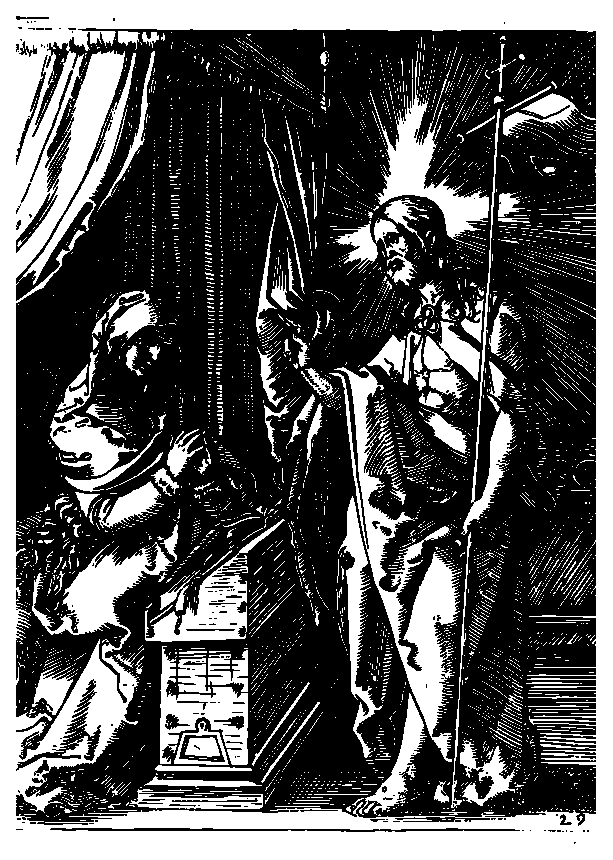
\includegraphics[width=103mm, height=135.046mm]{Prayers/Prayer.eps}
    \caption{\textsc{\Huge{Prayers \& Thanksgivings}}}
\end{figure}
\fancyhead[RO,LE]{}
\fancyhead[RE,LO]{}
\fancyhead[C]{{\LARGE Prayers}}\label{prayers}
\phantomsection
\addcontentsline{toc}{section}{Prayers}
%Uniquely 1928 Prayers are often omitted.

%\begin{rubric}
%To be used before the Prayer for all Conditions of Men, or, when that is not said, before the final Prayer of Thanksgiving or of Blessing, or before the Grace.
%\end{rubric}
%\begin{multicols}{2}
\subsection{Prayers for the United States of America}
%Prayer for the President of the United States is moved out of the Offices, into the Prayers section, together with the Prayers for the King, since it is not certain which will be needful.
\subsubsection{For the President of the United States, and all in Civil Authority}
\begin{inhead}
	\P{ }During Morning Prayer.
\end{inhead}
\lett{O}{Lord}, our heavenly Father, the high and mighty Ruler of the universe, who dost from thy throne behold all the dwellers upon earth; Most heartily we beseech thee, with thy favour to behold and bless thy servant \textsc{the President of the United States}, and all others in authority; and so replenish them with the grace of thy Holy Spirit, that they may always incline to thy will, and walk in thy way. Endue them plenteously with heavenly gifts; grant them in health and prosperity long to live; and finally, after this life, to attain everlasting joy and felicity; through Jesus Christ our Lord. \textit{Amen.}


\vspace{0.25\baselineskip}

\begin{inhead}
	\P{ }or this, during Morning Prayer.
\end{inhead}

\vspace{0.25\baselineskip}

\lett{O}{Lord} our Governor, whose glory is in all the world; We commend this nation to thy merciful care, that being guided by thy Providence, we may dwell secure in thy peace. Grant to \textsc{the President of the United States}, and to all in Authority, wisdom and strength to know and to do thy will. Fill them with the love of truth and righteousness; and make them ever mindful of their calling to serve this people in thy fear; through Jesus Christ our Lord, who liveth and reigneth with thee and the Holy Ghost, one God, world without end. \textit{Amen.}


\vspace{0.25\baselineskip}

\begin{inhead}
	\P{ }During Evening Prayer.
\end{inhead}

\vspace{0.25\baselineskip}


\lett{A}{lmighty} God, whose kingdom is everlasting and power infinite; Have mercy upon this whole land; and so rule the hearts of thy servants \textsc{the President of the United States}, \textit{The Governor of this State}, and all others in authority, that they, knowing whose ministers they are, may above all things seek thy honour and glory; and that we and all the People, duly considering whose authority they bear, may faithfully and obediently honour them, according to thy blessed Word and ordinance; through Jesus Christ our Lord, who with thee and the Holy Ghost liveth and reigneth ever, one God, world without end. \textit{Amen.}

\subsubsection{For Congress}

\begin{rubric}
To be used during their Session.
\end{rubric}
\lett{M}{ost} gracious God, we humbly beseech thee, as for the people of these United States in general, so especially for their Senate and Representatives in Congress assembled; that thou wouldest be pleased to direct and prosper all their consultations, to the advancement of thy glory, the good of thy Church, the safety, honour, and welfare of thy people; that all things may be so ordered and settled by their endeavours, upon the best and surest foundations, that peace and happiness, truth and justice, religion and piety, may be established among us for all generations. These and all other necessaries, for them, for us, and thy whole Church, we humbly beg in the Name and mediation of Jesus Christ, our most blessed Lord and Saviour. \textit{Amen.}

\subsubsection{For a State Legislature}

\lett{O}{God,} the fountain of wisdom, whose statutes are good and gracious and whose law is truth; We beseech thee so to guide and bless the Legislature of this \textit{State,} that it may ordain for our governance only such things as please thee, to the glory of thy Name and the welfare of the people; through Jesus Christ, thy Son, our Lord. \textit{Amen.}

\subsubsection{For Courts of Justice}

\lett{A}{lmighty} God, who sittest in the throne judging right; We humbly beseech thee to bless the courts of justice and the magistrates in all this land; and give unto them the spirit of wisdom and understanding, that they may discern the truth and impartially administer the law in the fear of thee alone; through him who shall come to be our judge, thy Son, our Saviour, Jesus Christ. \textit{Amen.}

%Army changed to Military to broaden it to all forces.
\subsubsection{For the Military}
\lett{O}{Lord} God of Hosts, stretch forth, we pray thee, thine almighty arm to strengthen and protect the Soldiers, Sailors, Marines, Airmen, Coast Guardsmen, and Guardians of our country; Support them in the day of battle, and in the time of peace keep them safe from all evil; endue them with courage and loyalty; and grant that in all things they may serve without reproach; through Jesus Christ our Lord. \textit{Amen.}

\vspace{0.25\baselineskip}

\begin{inhead}
	\P{ }or this.
\end{inhead}

\vspace{0.25\baselineskip}

\lett{H}{eavenly} Father, we commend to thy gracious care and keeping all the men and women in our Armed Forces at home and abroad. Defend them day by day with thy heavenly grace; strengthen them in their trials and temptations; give them courage to face the perils that beset them; and help them to know that none can pluck out of thy hand those who put their trust in thee; through Jesus Christ our Lord. \textit{Amen.}

%Omitted, because there is the prayer for those at sea.
%\subsubsection{For the Navy}
%\lett{O}{Eternal} Lord God, who alone spreadest out the heavens, and rulest the raging of the sea; Vouchsafe to take into thy almighty and most gracious protection our country's Navy, and all who serve therein. Preserve them from the dangers of the sea, and from the violence of the enemy; that they may be a safeguard unto the United States of America, and a security for such as pass on the seas upon their lawful occasions; that the inhabitants of our land may in peace and quietness serve thee our God, to the glory of thy Name; through Jesus Christ our Lord. \textit{Amen.}

%\subsubsection{For Our Country}
%\lett{A}{lmighty} God, who hast given us this good land for our heritage; We humbly beseech thee that we may always prove ourselves a people mindful of thy favour and glad to do thy will. Bless our land with honourable industry, sound learning, and pure manners. Save us from violence, discord, and confusion; from pride and arrogancy, and from every evil way. Defend our liberties, and fashion into one united people the multitudes brought hither out of many kindreds and tongues. Endue with the spirit of wisdom those to whom in thy Name we entrust the authority of government, that there may be justice and peace at home, and that, through obedience to thy law, we may show forth thy praise among the nations of the earth. In the time of prosperity, fill our hearts with thankfulness, and in the day of trouble, suffer not our trust in thee to fail; all which we ask through Jesus Christ our Lord. \textit{Amen.}

%MANUAL ADJUSTMENT:
\clearpage
\subsection{Prayers for Canada \& Commonwealth}
\subsubsection{For the King's Majesty}
\lett{O}{Lord}, our heavenly Father, high and mighty, King of kings, Lord of lords, the only Ruler of princes, who dost from thy throne behold all the dwellers upon earth: Most heartily we beseech thee with thy favour to behold our most gracious Sovereign Lord, King \textsc{\textit{Charles}}; and so replenish him with the grace of thy Holy Spirit, that he may alway incline to thy will, and walk in thy way. Endue him plenteously with heavenly gifts; grant him in health and wealth long to live; strengthen him that he may vanquish and overcome all his enemies; and finally after this life he may attain everlasting joy and felicity; through Jesus Christ our Lord. \textit{Amen.}

\subsubsection{For the Royal Family}
\lett{A}{lmighty} God, the fountain of all goodness, we humbly beseech thee to bless Queen \textit{Camilla}, \textit{William} Prince of Wales, the Princess of Wales, and all the Royal Family: Endue them with thy Holy Spirit; enrich them with thy heavenly grace; prosper them with all happiness; and bring them to thine everlasting kingdom; through Jesus Christ our Lord. \textit{Amen.}

%Empire changed to Commonwealth:
\subsubsection{For Parliament}
\lett{M}{ost} gracious God, we humbly beseech thee, as for this Commonwealth in general, so especially for the High Court of Parliament, \textit{the Parliament of this Dominion, and the Legislature of this Province,} under our most religious and gracious King at this time assembled: That thou wouldest be pleased to direct and prosper all their consultations to the advancement of thy glory, the good of thy Church, the safety, honour, and welfare of our Sovereign and his Dominions; that all things may be so ordered and settled by their endeavours, upon the best and surest foundations, that peace and happiness, truth and justice, religion and piety, may be established among us for all generations. These and all other necessaries, for them, for us, and thy whole Church, we humbly beg in the Name and Mediation of Jesus Christ our most blessed Lord and Saviour. \textit{Amen.}

%MANUAL ADJUSTMENT:
\clearpage
\subsubsection{For the Forces of the King}
\lett{O}{Lord} of Hosts, stretch forth, we pray thee, thine Almighty arm to strengthen and protect the forces of our King in every peril of sea, and land, and air; shelter them in the day of battle, and in time of peace keep them safe from all evil; endue them ever with loyalty and courage; and grant that in all things they may serve as seeing thee who art invisible; through Jesus Christ our Lord. \textit{Amen.}

\subsubsection{For the Commonwealth}
%Supplied from the English 1928's Prayer for the British Empire. I would love to use the 1962's Prayer, but I fear it may be in copyright still.
\lett{A}{lmighty} God, who rulest in the kingdom of men, and hast given to our Sovereign Lord, King \textsc{\textit{Charles}}, a great dominion in all parts of the earth: Draw together, we pray thee, in true fellowship the men of divers races, languages, and customs, who dwell therein, that, bearing one another's burdens, and working together in brotherly concord, they may fulfil the purpose of thy providence, and set forward thy everlasting kingdom. Pardon, we beseech thee our sins and shortcomings: keep far from us all selfishness and pride: and give us grace to employ thy good gifts of order and freedom to thy glory and the welfare of mankind; through Jesus Christ thy Son our Lord, to whom with thee and the Holy Ghost be all glory and dominion, world without end. \textit{Amen.}

\subsection{Prayers for the Church}
\subsubsection{For the Unity of God's People}
\lett{O}{God,} the Father of our Lord Jesus Christ, our only Saviour, the Prince of Peace; Give us grace seriously to lay to heart the great dangers we are in by our unhappy divisions. Take away all hatred and prejudice, and whatsoever else may hinder us from godly union and concord: that as there is but one Body and one Spirit, and one hope of our calling, one Lord, one Faith, one Baptism, one God and Father of us all, so we may be all of one heart and of one soul, united in one holy bond of truth and peace, of faith and charity, and may with one mind and one mouth glorify thee; through Jesus Christ our Lord. \textit{Amen.}

%MANUAL ADJUSTMENT:
\clearpage
\subsubsection{For those who are to be admitted into Holy Orders}

\begin{rubric}
To be used in the Weeks preceding the stated Times of Ordination.
\end{rubric}
\lett{A}{lmighty} God, our heavenly Father, who hast purchased to thyself an universal Church by the precious blood of thy dear Son; Mercifully look upon the same, and at this time so guide and govern the minds of thy servants the Bishops and Pastors of thy flock, that they may lay hands suddenly on no man, but faithfully and wisely make choice of fit persons, to serve in the sacred Ministry of thy Church, And to those who shall be ordained to any holy function, give thy grace and heavenly benediction; that both by their life and doctrine they may show forth thy glory, and set forward the salvation of all men; through Jesus Christ our Lord. \textit{Amen.}

\vspace{0.25\baselineskip}

\begin{inhead}
	\P{ }or this.
\end{inhead}

\vspace{0.25\baselineskip}

\lett{A}{lmighty} God, the giver of all good gifts, who of thy divine providence hast appointed divers Orders in thy Church; Give thy grace, we humbly beseech thee, to all those who are to be called to any office and administration in the same; and so replenish them with the truth of thy doctrine, and endue them with innocency of life, that they may faithfully serve before thee, to the glory of thy great Name, and the benefit of thy holy Church; through Jesus Christ our Lord. \textit{Amen.}


\subsubsection{For the Increase of the Ministry}

\lett{O}{almighty} God, look mercifully upon the world which thou hast redeemed by the blood of thy dear Son, and incline the hearts of many to dedicate themselves to the sacred ministry of thy Church; through the same thy Son Jesus Christ our Lord. \textit{Amen.}

%The 1928 unnecessarily softens the collect here. The 1928 is removed in preference for the 1892.
\subsubsection{For Missions}

\lett{O}{God,} who hast made of one blood all nations of men for to dwell on the face of the whole earth, and didst send thy blessed Son to preach peace to them that are far off and to them that are nigh; Grant that all men everywhere may seek after thee and find thee. Bring the nations into thy fold, and add the heathen to thine inheritance. And we pray thee shortly to accomplish the number of thine elect, and to hasten thy kingdom; through the same Jesus Christ our Lord. \textit{Amen.}

%MANUAL ADJUSTMENT
%\vfill

%	\begin{figure}[H]
%	    \centering
%	    \includegraphics[scale=0.125]{tailpiece/ChurchPiece.eps}
%	\end{figure}

\clearpage
\subsection{Prayers in Times of Illness}

\subsubsection{In Time of Great Sickness and Mortality}
%The 1928 shows the American disregard for wrath and repentance. Reverted to the 1892.
\lett{O}{almighty} God, the Lord of life and death, of sickness and health Regard our supplications, we humbly beseech thee; and, thou hast thought fit to visit us for our sins with great sickness and mortality, in the midst of thy judgment, O Lord, remember mercy. Have pity upon us miserable sinners, and withdraw from us the grievous sickness with which we are afflicted. May this thy fatherly correction have its due influence upon us, by leading us to consider how frail and uncertain our life is; that we may apply our hearts unto that heavenly wisdom which in the end will bring us to everlasting life; through Jesus Christ our Lord. \textit{Amen.}

\subsubsection{For a Sick Person}

\lett{O}{Father} of mercies and God of all comfort, our only help in time of need; We humbly beseech thee to behold, visit, and relieve thy sick \textit{servant} \textit{N.} for whom our prayers are desired. Look upon \textit{him} with the eyes of thy mercy; comfort \textit{him} with a sense of thy goodness; preserve \textit{him} from the temptations of the enemy; and give \textit{him} patience under \textit{his} affliction. In thy good time, restore \textit{him} to health, and enable \textit{him} to lead the residue of \textit{his} life in thy fear, and to thy glory; and grant that finally \textit{he} may dwell with thee in life everlasting; through Jesus Christ our Lord. \textit{Amen.}

%\subsubsection{For a Sick Child}
%\lett{O}{heavenly} Father, watch with us, we pray thee, over the sick child for whom our prayers are offered, and grant that \textit{he} may be restored to that perfect health which it is thine alone to give; through Jesus Christ our Lord. \textit{Amen.}

\subsection{Prayers in Times of Other Necessities}

\subsubsection{For Fruitful Seasons}

\begin{rubric}
	{To be used on Rogation Sunday and the Rogation Days}
\end{rubric}
\lett{A}{lmighty} God, who hast blessed the earth that it should be fruitful and bring forth whatsoever is needful for the life of man, and hast commanded us to work with quietness, and eat our own bread; Bless the labours of the husbandman, and grant such seasonable weather that we may gather in the fruits of the earth, and ever rejoice in thy goodness, to the praise of thy holy Name; through Jesus Christ our Lord. \textit{Amen.}

\vspace{0.25\baselineskip}

\begin{inhead}
	\P{ }or this.
\end{inhead}

\vspace{0.25\baselineskip}

\lett{O}{gracious} Father, who openest thine hand and fillest all things living with plenteousness; We beseech thee of thine infinite goodness to hear us, who now make our prayers and supplications unto thee. Remember not our sins, but thy promises of mercy. Vouchsafe to bless the lands and multiply the harvests of the world. Let thy breath go forth that it may renew the face of the earth. Show thy loving-kindness, that our land may give her increase; and so fill us with good things that the poor and needy may give thanks unto thy Name; through Christ our Lord. \textit{Amen.}

\subsubsection{For Rain}

\lett{O}{God,} heavenly Father, who by thy Son Jesus Christ hast promised to all those who seek thy kingdom, and the righteousness thereof, all things necessary to their bodily sustenance; Send us, we beseech thee, in this \textls[-15]{our necessity, such moderate rain and showers, that we may receive the fruits of the earth to our comfort, and to thy honour; through Jesus Christ our Lord. \textit{Amen.}}

%The American tendency to shy away from God's wrath has corrupted this prayer. The 1549 form is restored.
\subsubsection{For Fair Weather}
\lett{O}{Lord} God, which for the sin of man didst once drown all the world, except eight persons, and afterward of thy great mercy, didst promise never to destroy it so again: We humbly beseech thee, that although we for our iniquities have worthily deserved this plague of rain and waters, yet, upon our true repentance, thou wilt send us such weather whereby we may receive the fruits of the earth in due season, and learn both by the punishment to amend our lives, and by the granting of our petition to give thee praise and glory: Through Jesu Christ our Lord. \textit{Amen.}

\subsubsection{For Every Man in his Work}
\lett{A}{lmighty} God, our heavenly Father, who declarest thy glory and showest forth thy handiwork in the heavens and in the earth; Deliver us, we beseech thee, in our several callings, from the service of mammon, that we may do the work which thou givest us to do, in truth, in beauty, and in righteousness, with singleness of heart as thy servants, and to the benefit of our fellow men; for the sake of him who came among us as one that serveth, thy Son, Jesus Christ our Lord. \textit{Amen.}

\subsubsection{For Christian Justice}
\lett{A}{lmighty} God, who hast created man in thine own image; Grant us grace fearlessly to contend against evil, and to make no peace with oppression; and, that we may reverently use our freedom, help us to employ it in the maintenance of justice among men and nations, to the glory of thy holy Name; through Jesus Christ our Lord. \textit{Amen.}

\subsubsection{In Time of Dearth and Famine}
\lett{O}{God,} heavenly Father, whose gift it is that the rain doth fall, and the earth bring forth her increase; Behold, we beseech thee, the afflictions of thy people; increase the fruits of the earth by thy heavenly benediction; and grant that the scarcity and dearth, which we now most justly suffer for our sins, may, through thy goodness, be mercifully turned into plenty; for the love of Jesus Christ our Lord, to whom, with thee and the Holy Ghost, be all honour and glory, now and for ever. \textit{Amen.}

\subsubsection{In Time of War and Tumults}
%The 1928 shows an American discomfort for condemnation. For greater conformity with the Canadian, reverted to 1662.
\lett{O}{almighty} God, King of all kings, and Governor of all things, whose power no creature is able to resist, to whom it belongeth justly to punish sinners, and to be merciful to those who truly repent; Save and deliver us, we humbly beseech thee, from the hands of our enemies; abate their pride, assuage their malice, and confound their devices; that we, being armed with thy defence, may be preserved evermore from all perils, to glorify thee, who art the only giver of all victory; through the merits of thy Son, Jesus Christ our Lord. \textit{Amen.}

\subsubsection{In Time of Calamity}
\lett{O}{God,} merciful and compassionate, who art ever ready to hear the prayers of those who put their trust in thee; Graciously hearken to us who call upon thee, and grant us thy help in this our need; through Jesus Christ our Lord. \textit{Amen.}

\subsubsection{For a Person under Affliction}

\lett{O}{merciful} God, and heavenly Father, who hast taught us in thy holy Word that thou dost not willingly afflict or grieve the children of men; Look with pity, we beseech thee, upon the sorrows of thy \textit{servant} for whom our prayers are offered. Remember \textit{him}, O Lord, in mercy; endue \textit{his} soul with patience; comfort \textit{him} with a sense of thy goodness; lift up thy countenance upon \textit{him}, and give \textit{him} peace; through Jesus Christ our Lord. \textit{Amen.}

%MANUAL ADJUSTMENT:
\clearpage
\subsubsection{For a Person, or Persons, going to Sea}

\lett{O}{eternal} God, who alone spreadest out the heavens, and rulest the raging of the sea; We commend to thy almighty protection, thy \textit{servant}, for whose preservation on the great deep our prayers are desired. Guard \textit{him}, we beseech thee, from the dangers of the sea, from sickness, from the violence of enemies, and from every evil to which \textit{he} may be exposed. Conduct \textit{him} in safety to the haven where \textit{he} would be, with a grateful sense of thy mercies; through Jesus Christ our Lord. \textit{Amen.}

\subsubsection{For Prisoners}

\lett{O}{God,} who sparest when we deserve punishment, and in thy wrath rememberest mercy; We humbly beseech thee, of thy goodness, to comfort and succour all prisoners (especially those who are condemned to die). Give them a right understanding of themselves, and of thy promises; that, trusting wholly in thy mercy, they may not place their confidence anywhere but in thee. Relieve the distressed, protect the innocent, awaken the guilty; and forasmuch as thou alone bringest light out of darkness, and good out of evil, grant to these thy servants, that by the power of thy Holy Spirit they may be set free from the chains of sin, and may be brought to newness of life; through Jesus Christ our Lord. \textit{Amen.}

\begin{inhead}
	\P{ }or this.
\end{inhead}

\vspace{0.25\baselineskip}

%Supplied from the 1892 for those about to receive the Death Penalty.
\lett{O}{most} gracious and merciful God, we earnestly beseech thee to have pity and compassion upon these persons recommended to our prayers, who now lie under the sentence of the law and are appointed to die. Visit them, O Lord, with thy mercy and salvation convince them of the miserable condition they are in, by their sins and wickedness; and let thy powerful grace produce in them such a godly sorrow, and sincere repentance, as thou wilt be pleased to accept. Give them a strong and lively faith in thy Son, our blessed Saviour and make it effectual to the salvation of their souls. O Lord, in judgment remember mercy and whatever sufferings they are to endure in this world, yet deliver them, O God, from the bitter pains of eternal death. Pardon their sins, and save their souls, for the sake and merits of thy dear Son, our blessed Saviour and Redeemer. \textit{Amen.}



%\subsection{Prayers for the Christian Life}
%\subsubsection{For Schools, Colleges, and Universities}
%\lett{A}{lmighty} God, we beseech thee, with thy gracious favour, to behold our universities, colleges, and schools, that knowledge may be increased among us, and all good learning flourish and abound; bless all who teach and all who learn; and grant that in humility of heart they may ever look unto thee, who art the fountain of all wisdom; through Jesus Christ our Lord. \textit{Amen.}

%\subsubsection{For Religious Education}
%\lett{A}{lmighty} God, our Heavenly Father, who hast committed to thy Holy Church the care and nurture of thy children; Enlighten with thy wisdom those who teach and those who learn; that, rejoicing in the knowledge of thy truth, they may worship thee and serve thee from generation to generation; through Jesus Christ our Lord. \textit{Amen.}

%\subsubsection{For Children}
%\lett{O}{lord} Jesus Christ, who dost embrace children with the arms of thy mercy, and dost make them living members of thy Church; Give them grace, we pray thee, to stand fast in thy faith, to obey thy word, and to abide in thy love; that being made strong by thy Holy Spirit they may resist temptation and overcome evil; and may rejoice in the life that now is, and dwell with thee in the life that is to come; through thy merits, O merciful Saviour, who with the Father and the Holy Ghost livest and reignest one God, world without end. \textit{Amen.}

%\subsubsection{For Those About to be Confirmed}
%\lett{O}{God,} who through the teaching of thy Son Jesus Christ didst prepare the disciples for the coming of the Comforter; Make ready, we beseech thee, the hearts and minds of thy servants who at this time are seeking to be strengthened by the gift of the Holy Spirit through the laying on of hands, that, drawing near with penitent and faithful hearts, they may evermore be filled with the power of his divine indwelling; through the same Jesus Christ our Lord. \textit{Amen.}

%\subsubsection{For Christian Service}
%\lett{O}{Lord,} our heavenly Father, whose blessed Son came not to be ministered unto, but to minister; We beseech thee to bless all who, following in his steps, give themselves to the service of their fellow men. Endue them with wisdom, patience, and courage, that they may strengthen the weak and raise up those who fall; and, being inspired by thy love, may worthily minister in thy Name to the suffering, the friendless, and the needy; for the sake of him who laid down his life for us, the same thy Son, our Saviour, Jesus Christ. \textit{Amen.}


%MANUAL ADJUSTMENT:
\clearpage
\subsection{Prayers for the Dead}\label{dead}
\subsubsection{For All the Faithful Departed}
\lett{O}{God,} the Creator and Redeemer of all the faithful: grant unto the souls of thy servants and handmaids the remission of all their sins; that through devout supplications they may obtain the pardon they have always desired. Who with God the Father in the unity of the Holy Spirit livest and reignest God, world without end. \textit{Amen.}

\subsubsection{On the Day of Burial}

\lett{A}{bsolve}, O Lord, we beseech thee, the soul of thy \textit{servant N.}, that being dead to the world \textit{he} may live unto thee: and whatsoever \textit{he} hath done amiss in \textit{his} earthly conversation through frailty of the flesh, do thou wipe away by the pardon of thy merciful goodness. Through.

\subsubsection{For a Priest Departed}

\lett{O}{God,} who hast made thy \textit{servant N.} to flourish among the Ministers of Apostolic Succession in the honourable office of a Priest: grant, we beseech thee, that \textit{he} may also be joined with them in a perpetual fellowship. Through.

\subsubsection{Another Collect for a Priest Departed}

\lett{G}{rant}, we beseech thee, O Lord: that the soul of thy servant the Priest \textit{N.}, whom while dwelling in this world thou didst adorn with holy gifts, may ever rejoice with glory in the heavenly mansions. Through.

\subsubsection{For a Father and Mother}
\lett{O}{God,} who hast bidden us to honour our father and mother: of thy mercy have compassion on the \textit{souls} of \textit{my father and mother}; forgive \textit{their} sins, and grant that \textit{I} may behold \textit{them} in the joy of eternal brightness. Through.

\subsubsection{For Many Deceased}
\lett{O}{God,} whose nature and property is ever to have mercy and to forgive: have compassion on the souls of thy servants and handmaids, and grant them the remission of all their sins; that being delivered from the bonds of mortality, they may be worthy to pass over into life. Through.

\subsubsection{Another Collect for Many Deceased}
\lett{G}{rant}, we beseech thee, O Lord, to the souls of thy servants and handmaids thy perpetual mercy: and let it profit them in eternity that they hoped and believed in thee. Through.

\subsubsection{For a Man Departed}
\lett{I}{ncline} thine ear, O Lord, unto our prayers, wherein we humbly entreat thy mercy: that thou wouldest appoint unto the soul of thy servant \textit{N.}, which thou hast bidden to depart out of this world, a place in the land of life and peace; and wouldest make him a partaker with thy Saints. Through.

\subsubsection{For a Woman Departed}
\lett{W}{e} beseech thee, O Lord, of thy loving kindness have mercy upon the soul of thine handmaid \textit{N.}: and now that she is released from the contagion of mortality, do thou restore her portion in everlasting salvation. Through.

\subsubsection{Through the Year}
\lett{O}{God,} who hast made thy servants to flourish among the Ministers of Apostolic Succession in the honourable offices of Bishopric and Priesthood: grant, we beseech thee, that they may also be joined with them in a perpetual fellowship.

\begin{inhead}
	\P{ }or this.
\end{inhead}

\vspace{0.25\baselineskip}

\lett{O}{God,} the Giver of pardon and the Author of man's salvation: we humbly beseech thy mercy to grant that the \textit{brethren}, kinsfolk, and benefactors of our Congregation who have departed out of this world, blessed Mary ever Virgin and all thy Saints praying for them, may attain to the fellowship of everlasting blessedness.

\vspace{0.25\baselineskip}

\begin{inhead}
	\P{ }or this.
\end{inhead}

\vspace{0.25\baselineskip}

\lett{O}{God,} the Creator and Redeemer of all the faithful: grant unto the souls of thy servants and handmaids the remission of all their sins; that through devout supplications they may obtain the pardon they have always desired. Who with God the Father, in the unity of the Holy Spirit, livest and reignest God, world without end. \textit{Amen.}

%MANUAL ADJUSTMENT:
\clearpage
\subsection{Additional Collects}\label{AdditionalCollects}
\begin{rubric}
    These Collects are said for the conclusion of Antecommunion. They may be said after the Collects of Morning and Evening Prayer, at the discretion of the Minister.
\end{rubric}
\lett{O}{Lord} Jesu Christ, who saidst unto thine Apostles, Peace I leave with you, my peace I give unto you; Regard not our sins, but the faith of thy Church; and grant to it that peace and unity which is according to thy will, who livest and reignest with the Father and the Holy Ghost, one God, world without end. \textit{Amen.}

\lett{A}{ssist} us mercifully, O Lord, in these our supplications and prayers, and dispose the way of thy servants towards the attainment of everlasting salvation; that, among all the changes and chances of this mortal life, they may ever be defended by thy most gracious and ready help; through Jesus Christ our Lord. \textit{Amen.}

\lett{G}{rant,} we beseech thee, Almighty God, that the words which we have heard this day with our outward ears, may, through thy grace, be so grafted inwardly in our hearts, that they may bring forth in us the fruit of good living, to the honour and praise of thy Name; through Jesus Christ our Lord. \textit{Amen.}

\lett{D}{irect} us, O Lord, in all our doings, with thy most gracious favour, and further us with thy continual help; that in all our works begun, continued, and ended in thee, we may glorify thy holy Name, and finally, by thy mercy, obtain everlasting life; through Jesus Christ our Lord. \textit{Amen.}

\lett{A}{lmighty} God, the fountain of all wisdom, who knowest our necessities before we ask, and our ignorance in asking; We beseech thee to have compassion upon our infirmities; and those things which for our unworthiness we dare not, and for our blindness we cannot ask, vouchsafe to give us, for the worthiness of thy Son Jesus Christ our Lord. \textit{Amen.}

\lett{A}{lmighty} God, who hast promised to hear the petitions of those who ask in thy Son's Name; We beseech thee mercifully to incline thine ears to us who have now made our prayers and supplications unto thee; and grant that those things which we have faithfully asked according to thy will, may effectually be obtained, to the relief of our necessity, and to the setting forth of thy glory; through Jesus Christ our Lord. \textit{Amen.}
%\end{multicols}
%Inspired by the English Office Noted. Translation from the 1933 English Missal.
%\lett{D}{efend} us, O Lord, we beseech thee, from all dangers of mind and body: and at the intercession of the blessed and glorious Mother of God, Mary ever Virgin, with blessed Joseph, thy blessed Apostles Peter and Paul, (blessed \textit{N.},) and all the Saints, graciously grant us health and peace; that all adversities and errors being done away, thy Church may serve thee in freedom and quietness. Through the same Jesus Christ thy Son, our Lord, who liveth and reigneth with thee and the Holy Ghost, ever one God, world without end. \textit{Amen.}

%Since the 1928 BCP has a Bidding Prayer unique to itself, clearly incorporating elements of Laudian and Andrewian Branch Theory (as happens in the Prayer for the Church excluded from this Book), the following from King Henry VIII's reign is here provided, along with further bidding for the dead from the Manuale (https://www.google.com/books/edition/Forms_of_Bidding_Prayer_with_Introductio/ptkDAAAAQAAJ?hl=en&gbpv=1&dq=Forms+of+Bidding+Prayer&printsec=frontcover).

%MANUAL ADJUSTMENT:
\clearpage
\subsection{A Bidding Prayer}

\begin{rubric}
	{To be used to preface Sermons, or on Special Occasions.}
\end{rubric}

\lett{A}{fter} a laudable custom of our Mother holy Church, ye shall kneel down, moving your hearts unto Almighty God, and making your special prayers for the three estates, concerning all Christian people, that is, for the Spirituality, the Temporality, and the souls departed.

\lett{F}{irst} for all archbishops, and bishops, and in special for my Lord \textit{Archbishop} of \textit{these United States}, your \textit{Metropolitan,} and also for my Lord \textit{Bishop} of this \textit{Diocese}, and in general for all parsons, vicars, and parish priests having cure of souls, with the ministers of Christ's Church, as well monastic as not monastic.

\lett{S}{econdly,} ye shall pray for the unity and peace of all Christian Realms. And for the noble Realm of \textit{America}, and for \textit{the President of these United States}; that Almighty God may send them grace, so to govern and rule the land, that it may be pleasing unto Almighty God, wealth and profit to the land, and salvation to their souls. Also ye shall pray for all those that have honoured the Church with light, lamp, vestment, or bell, or with any other ornaments, by which the service of Almighty God is the better maintained and kept. Furthermore ye shall pray for all true travellers and tillers of the earth, that truly and duly done their duty to God and holy Church, as they be bound to do.

Also ye shall pray for all manner of fruits that be done upon the ground, or shall be that Almighty God of his great pity and mercy may send such weather, that it may come to the sustenance of man. Ye shall pray also for all those that be in debt or deadly sin, that Almighty God may give them grace to come out thereof, and the sooner by our prayer. Also ye shall pray for all those that be sick or diseased, either in body or in soul, that the Almighty would send them the thing that is most profitable as well bodily as ghostly. Also ye shall pray for all pilgrims, and palmers, that have taken the way to Rome, to Saint James of Jerusalem, or to any other place: that Almighty God may give them grace to go safe, and to come safe, and give us grace to have part of their prayers, and they part of ours. Also ye shall pray for the holy Cross, that is in possession and hands of unrightful people; that God Almighty may send it into the hands of Christian people when it pleaseth him. Furthermore I commit unto your devout prayers, all women that be in our ladies' bonds: that Almighty God may send them grace, the child to receive the Sacrament of Baptism, and the mother purification. Also ye shall pray for the good man and woman, that this day giveth bread to make the holy loaf, and for all those that first began it, and them that longest continue. For these and for all true Christian people, every man and woman say the Lord's Prayer and the Angelic Salutation.

\begin{rubric}
    The Priest and the People say,
\end{rubric}

\lett{O}{ur} Father, who art in heaven, Hallowed be thy Name. Thy kingdom come. Thy will be done on earth, As it is in heaven. Give us this day our daily bread. And forgive us our trespasses, As we forgive those who trespass against us. And lead us not into temptation; But deliver us from evil: For thine is the kingdom, and the power, and the glory, for ever and ever. Amen.
\par\noindent
\lett{H}{ail} Mary, full of grace; The Lord is with thee; Blessed art thou amongst women, And blessed is the fruit of thy womb, Jesus. Holy Mary, Mother of God, Pray for us sinners, now and at the hour of our death. Amen.
\begin{rubric}
    The Priest then says,
\end{rubric}
\lett{Y}{e} shall make a special prayer for your fathers' souls, for your mothers' souls, godfathers' souls and godmothers' souls, brothers' souls and sisters' souls, and for all your elders' souls, and for all the souls, that ye or I be bound to pray for, and specially for all the souls whose bones are buried in this Church or in this Churchyard, or in any other holy place, and especially for all the souls that bid the great mercy of Almighty God, that God for his great mercy release them of their pain, if it be his blessed will, and that our prayers may sum what stand them in stead; every man and woman of your charity help them with the Lord's Prayer and the Angelic Salutation.
\begin{rubric}
    The Priest and the People again say,
\end{rubric}
\lett{O}{ur} Father, who art in heaven, Hallowed be thy Name. Thy kingdom come. Thy will be done on earth, As it is in heaven. Give us this day our daily bread. And forgive us our trespasses, As we forgive those who trespass against us. And lead us not into temptation; But deliver us from evil: For thine is the kingdom, and the power, and the glory, for ever and ever. Amen.
\par\noindent
\lett{H}{ail} Mary, full of grace; The Lord is with thee; Blessed art thou amongst women, And blessed is the fruit of thy womb, Jesus. Holy Mary, Mother of God, Pray for us sinners, now and at the hour of our death. Amen.
%\begin{rubric}
%    The Priest and the People then conclude the Bidding of the Bedes by saying the Lord's Prayer and Angelic Salutation once more.
%\end{rubric}

%\lett{O}{ur} Father, who art in heaven, Hallowed be thy Name. Thy kingdom come. Thy will be done on earth, As it is in heaven. Give us this day our daily bread. And forgive us our trespasses, As we forgive those who trespass against us. And lead us not into temptation; But deliver us from evil: For thine is the kingdom, and the power, and the glory, for ever and ever. Amen.

%\lett{H}{ail} Mary, full of grace; The Lord is with thee; Blessed art thou amongst women, And blessed is the fruit of thy womb, Jesus. Holy Mary, Mother of God, Pray for us sinners, now and at the hour of our death. Amen.

%MANUAL ADJUSTMENT

\vfill

	\begin{figure}[H]
	    \centering
	    
\includegraphics[width=36.107mm,height=30mm]{tailpiece/Fountain.eps}
	\end{figure}

\clearpage
\fancyhead[RO,LE]{}
\fancyhead[RE,LO]{}
\fancyhead[C]{{\LARGE Thanksgivings}}\label{thanksgiving}
\phantomsection
\addcontentsline{toc}{section}{Thanksgivings}
%\begin{rubric}
%	To be used after the General Thanksgiving, or, when that is not said, before the final Prayer of Blessing or the Benediction.
%\end{rubric}
%\begin{multicols}{2}
\subsection{A Thanksgiving to Almighty God for the Fruits of the Earth and all the other Blessings of his merciful Providence}
\lett{M}{ost} gracious God, by whose knowledge the depths are broken up, and the clouds drop down the dew; We yield thee unfeigned thanks and praise for the return of seed-time and harvest, for the increase of the ground and the gathering in of the fruits thereof, and for all the other blessings of thy merciful providence bestowed upon this nation and people. And, we beseech thee, give us a just sense of these great mercies; such as may appear in our lives by an humble, holy, and obedient walking before thee all our days; through Jesus Christ our Lord, to whom, with thee and the Holy Ghost, be all glory and honour, world without end. \textit{Amen.}

\subsection{The Thanksgiving of Women after Child-birth}
\begin{rubric}
	To be said when any Woman, being present in Church, shall have desired to return thanks to Almighty God for her safe deliverance.
\end{rubric}%Changed servant to handmaid

\lett{O}{almighty} God, we give thee humble thanks for that thou hast been graciously pleased to preserve, through the great pain and peril of childbirth, this woman, thy handmaid, who desireth now to offer her praises and thanksgivings unto thee. Grant, we beseech thee, most merciful Father, that she, through thy help, may both faithfully live and walk according to thy will in this life present, and also may be partaker of everlasting glory in the life to come; through Jesus Christ our Lord. \textit{Amen.}

\subsection{For Rain}
\lett{O}{God,} our heavenly Father, by whose gracious providence the former and the latter rain descend upon the earth, that it may bring forth fruit for the use of man; We give thee humble thanks that it hath pleased thee to send us rain to our great comfort, and to the glory of thy holy Name; through Jesus Christ our Lord. \textit{Amen.}

%MANUAL ADJUSTMENT
\clearpage
\subsection{For Fair Weather}
\lett{O}{Lord} God, who hast justly humbled us by thy late visitation of us with immoderate rain and waters, and in thy mercy hast relieved and comforted our souls by this seasonable and blessed change of weather; We praise and glorify thy holy Name for this thy mercy, and will always declare thy loving-kindness from generation to generation; through Jesus Christ our Lord. \textit{Amen.}

\subsection{For Peace, and Deliverance from our Enemies}
\lett{O}{almighty} God, who art a strong tower of defence unto thy servants against the face of their enemies; We yield thee praise and thanksgiving for our deliverance from those great and apparent dangers wherewith we were compassed. We acknowledge in thy goodness that we were not delivered over as a prey unto them; beseeching thee still to continue such thy mercies towards us, that all the world may know that thou art our Saviour and mighty Deliverer; through Jesus Christ our Lord. \textit{Amen.}

\subsection{For Restoring Public Peace at Home}
\lett{O}{eternal} God, our heavenly Father, who alone makest men to be of one mind in a house, and stillest the outrage of a violent and unruly people; We bless thy holy Name, that it hath pleased thee to appease the seditious tumults which have been lately raised up amongst us; most humbly beseeching thee to grant to all of us grace, that we may henceforth obediently walk in thy holy commandments; and, leading a quiet and peaceable life in all godliness and honesty, may continually offer unto thee our sacrifice of praise and thanksgiving for these thy mercies towards us; through Jesus Christ our Lord. \textit{Amen.}

\subsection{For Deliverance from great Sickness and Mortality}
\lett{O}{Lord} God, who hast wounded us for our sins, and consumed us for our transgressions, by thy late heavy and dreadful visitation and now, in the midst of judgment remembering mercy, hast redeemed our souls from the jaws of death; We offer unto thy fatherly goodness ourselves, our souls and bodies which thou hast delivered, to be a living sacrifice unto thee, always praising and magnifying thy mercies in the midst of thy Church; through Jesus Christ our Lord. \textit{Amen.}

\subsection{For Recovery from Sickness}
\lett{O}{God,} who art the giver of life, of health, and of safety; We bless thy Name, that thou hast been pleased to deliver from \textit{his} bodily sickness this thy \textit{servant}, who now desireth to return thanks unto thee, in the presence of all thy people. Gracious art thou, O Lord, and full of compassion to the children of men. May \textit{his} heart be duly impressed with a sense of thy merciful goodness, and may \textit{he} devote the residue of \textit{his} days to an humble, holy, and obedient walking before thee; through Jesus Christ our Lord. \textit{Amen.}

\subsection{For a Child's Recovery from Sickness}
\lett{A}{lmighty} God and heavenly Father, we give thee humble thanks for that thou hast been graciously pleased to deliver from \textit{his} bodily sickness the child in whose behalf we bless and praise thy Name, in the presence of all thy people. Grant, we beseech thee, O gracious Father, that \textit{he}, through thy help, may both faithfully live in this world according to thy will, and also may be partaker of everlasting glory in the life to come; through Jesus Christ our Lord. \textit{Amen.}

\subsection{For a Safe Return from a Journey}
\lett{M}{ost} gracious Lord, whose mercy is over all thy works; We praise thy holy Name that thou hast been pleased to conduct in safety, through the perils of the great deep, (\textit{his} way,) this thy \textit{servant}, who now desireth to return \textit{his} thanks unto thee in thy holy Church. May \textit{he} be duly sensible of thy merciful providence towards \textit{him}, and ever express \textit{his} thankfulness by a holy trust in thee, and obedience to thy laws; through Jesus Christ our Lord. \textit{Amen.}
%\end{multicols}
%Litanies \& Offices
\cleardoublepage
\fancyhead[RE,LO]{}\fancyhead[RO,LE]{}
\fancyhead[C]{}
\thispagestyle{empty}
\phantomsection
\addcontentsline{toc}{chapter}{Litanies \& Offices}

\begin{figure}[H]
    \centering
    
\includegraphics[width=103mm, height=147.025mm]{Litanies/DavidRepentance.eps}
    \caption{\textsc{\Huge{Litanies \& Offices of the Church}}}
\end{figure}
\include{pages/Litanies/GreatLitany}
\fancyhead[RO,LE]{\textit{Penitential Office}}\label{penitential}
\fancyhead[RE,LO]{}
\section{A Penitential Office}
%From the 1928 Book of Common Prayer
\begin{secrubric}
%Language of rubric from the 1928 American is adjusted for readability
	On the First Day of Lent, the Penitential Office is read immediately after the Great Litany during Morning Prayer. It may also be used during Evening Prayer or as a separate Office.
\end{secrubric}
\begin{secrubric}
    The Penitential Office may be read at other times, at the discretion of the Minister.
\end{secrubric}
\begin{secrubric}
    The Minister and the People kneeling, then shall be said by them this Psalm following.
\end{secrubric}
\subsection{Psalm 51. \textit{Miserere mei, Deus}}
\lett{H}{ave} mercy upon me, O God, after thy great goodness~: according to the multitude of thy mercies do away mine offences.\par
\secondline{\psanum{2}Wash me throughly from my wickedness~: and cleanse me from my sin.}
\thirdline{\psanum{3}For I acknowledge my faults~: and my sin is ever before me.}
\psanum{4}Against thee only have I sinned, and done this evil in thy sight~: that thou mightest be justified in thy saying, and clear when thou art judged.\par
\psanum{5}Behold, I was shapen in wickedness~: and in sin hath my mother conceived me.\par
\psanum{6}But lo, thou requirest truth in the inward parts~: and shalt make me to understand wisdom secretly.\par
\psanum{7}Thou shalt purge me with hyssop, and I shall be clean~: thou shalt wash me, and I shall be whiter than snow.\par
\psanum{8}Thou shalt make me hear of joy and gladness~: that the bones which thou hast broken may rejoice.\par
\psanum{9}Turn thy face from my sins~: and put out all my misdeeds.\par
\psanum{10}Make me a clean heart, O God~: and renew a right spirit within me.\par
\psanum{11}Cast me not away from thy presence~: and take not thy holy Spirit from me.\par
\psanum{12}O give me the comfort of thy help again~: and stablish me with thy free Spirit.\par
\psanum{13}Then shall I teach thy ways unto the wicked~: and sinners shall be converted unto thee.\par
\psanum{14}Deliver me from blood-guiltiness, O God, thou that art the God of my health~: and my tongue shall sing of thy righteousness.\par
\psanum{15}Thou shalt open my lips, O Lord~: and my mouth shall shew thy praise.\par
\psanum{16}For thou desirest no sacrifice, else would I give it thee~: but thou delightest not in burnt-offerings.\par
\psanum{17}The sacrifice of God is a troubled spirit~: a broken and contrite heart, O God, shalt thou not despise.\par
\psanum{18}O be favourable and gracious unto Sion~: build thou the walls of Jerusalem.\par
\psanum{19}Then shalt thou be pleased with the sacrifice of righteousness, with the burnt-offerings and oblations~: then shall they offer young bullocks upon thine altar.\par
℣. Glory be to the Father, and to the Son, and to the Holy Ghost.\par
℟. As it was in the beginning, is now, and ever shall be, world without end. Amen.
\begin{rubric}
    If the Litany hath been already said, the Minister may pass at once to \blackrubric{O Lord, save thy servants; etc.}
\end{rubric}
\par\noindent
	\centerline{\rule{0.5\textwidth}{0.4pt}}
\par
    ℣. Lord, have mercy upon us.

    ℟. Christ, have mercy upon us.
    
    ℣. Lord, have mercy upon us.
    
\lett{O}{ur} Father who art in heaven, Hallowed be thy Name. Thy kingdom come. Thy will be done on earth, As it is in heaven. Give us this day our daily bread. And forgive us our trespasses, As we forgive those who trespass against us. And lead us not into temptation; But deliver us from evil. Amen.
\par\noindent
	\centerline{\rule{0.5\textwidth}{0.4pt}}
\par
    ℣. O Lord, save thy servants;

    ℟. That put their trust in thee.

    ℣. Send unto them help from above.

    ℟. And evermore mightily defend them.

    ℣. Help us, O God our Saviour.

    ℟. And for the glory of thy Name deliver us; be merciful to us sinners, for thy Name's sake.
    
    ℣. O Lord, hear our prayer.
    
    ℟. And let our cry come unto thee.

\letuspray
\lett{O}{Lord,} we beseech thee, mercifully hear our prayers, and spare all those who confess their sins unto thee; that they, whose consciences by sin are accused, by thy merciful pardon may be absolved; through Christ our Lord. \textit{Amen.}

\lett{O}{most} mighty God, and merciful Father, who hast compassion upon all men, and who wouldest not the death of a sinner, but rather that he should turn from his sin, and be saved; Mercifully forgive us our trespasses; receive and comfort us, who are grieved and wearied with the burden of our sins. Thy property is always to have mercy; to thee only it appertaineth to forgive sins. Spare us therefore, good Lord, spare thy people, whom thou hast redeemed; enter not into judgment with thy servants; but so turn thine anger from us, who meekly acknowledge our transgressions, and truly repent us of our faults, and so make haste to help us in this world, that we may ever live with thee in the world to come; through Jesus Christ our Lord. \textit{Amen.}

%Rubric language slightly adjusted for clarity.
\begin{rubric}
    Then shall the People say this that followeth, with the Minister.
\end{rubric}

\lett{T}{urn} thou us, O good Lord, and so shall we be turned. Be favourable, O Lord, Be favourable to thy people, Who turn to thee in weeping, fasting, and praying. For thou art a merciful God, Full of compassion, Long-suffering, and of great pity. Thou sparest when we deserve punishment, And in thy wrath thinkest upon mercy. Spare thy people, good Lord, spare them, And let not thine heritage be brought to confusion. Hear us, O Lord, for thy mercy is great, And after the multitude of thy mercies look upon us; Through the merits and mediation of thy blessed Son, Jesus Christ our Lord. \textit{Amen.}

\begin{rubric}
    Then the Minister shall say,
\end{rubric}

\lett{O}{God,} whose nature and property is ever to have mercy and to forgive; Receive our humble petitions; and though we be tied and bound with the chain of our sins, yet let the pitifulness of thy great mercy loose us; for the honour of Jesus Christ, our Mediator and Advocate. \textit{Amen.}

\lett{T}{he} Lord bless us, and keep us. The Lord make his face to shine upon us, and be gracious unto us. The Lord lift up his countenance upon us, and give us peace, both now and evermore. \textit{Amen.}
%\begin{center}
%    \textsc{Here endeth the Penitential Office.}
%\end{center}
\section{Sacrament of Penance}
\fancyhead[RO,LE]{\textit{Penance}}
%Penance comes from the Monastic Diurnal

\begin{multicols}{2}
\begin{rubric}
	The Pentient begins with the following.
\end{rubric}
Bless me, Father, for I have sinned.\par

℣. The Lord be in thy heart and upon thy lips, that so thou mayest worthily confess all thy sins; In the Name of the Father, {\ding{64}} and of the Son, and of the Holy Ghost. Amen.\par
\begin{rubric}
	{The Penitent then confesses his sins using the following or similar formula:}
\end{rubric}
\label{Confiteor}
I confess to God Almighty, to Blessed Mary Ever-Virgin, to blessed Michael the Archangel, to blessed John Baptist, to the holy Apostles Peter and Paul, to all the Saints, and to thee, Father, that I have sinned exceedingly in thought, word, and deed, by my fault, by my own fault, by my own most grievous fault,\par
Especially I accuse myself that since my last Confession, which was \inrub{Say how long} ago, I have committed the following sins. \inrub{Confess your sins and conclude with:}\par
For these and for all my other sins which I cannot now remember, I am heartily sorry, firmly purpose amendment, and humbly ask pardon of God; and of thee, my spiritual father, penance, counsel, and Absolution.\par
Wherefore I beg blessed Mary Ever-Virgin, blessed Michael the Archangel, blessed John Baptist, the holy Apostles Peter and Paul, all the Saints, and thee, father, to pray for me to the Lord our God.

\newcolumn

\begin{rubric}
	{Here the Priest gives penance, counsel, and then absolution saying,}
\end{rubric}
%\elcol{
\lett{A}{lmighty} God have mercy upon thee, forgive thee thy sins, and bring thee to everlasting life. \textit{Amen.}%}{\lett{M}{isere\smash{á}tur} tui omnípotens Deus, et dimíssis peccátis tuis, perdúcat te ad vitam {\ae}térnam. Amen.}
%\elcol{
\lett{T}{he} Almighty and merciful Lord grant thee pardon, {\ding{64}} absolution, and remission of thy sins. \textit{Amen.}%}{\lett{I}{ndulg\smash{é}ntiam,} {\ding{64}} absolutiónem, et remissiónem peccatórum tuórum tríbuat tibi omnípotens et miséricors Dóminus. Amen.}
\par\noindent
%	\centerline{\rule{0.5\textwidth}{0.4pt}}
%\par\noindent
%\elcol{Our Lord Jesus Christ absolves thee; and I, by his authority, absolve thee from every bond of excommunication, (suspension,) and interdict, so far as I have power, and thou hast need. I absolve thee from thy sins, in the Name of the Father, {\ding{64}} and of the Son, and of the Holy Ghost. Amen.}{Dóminus noster Jesus Christus te absólvat; et ego auctoritáte ipsíus te absólvo ab omni vínculo excommunicatiónis, (suspensiónis,) et interdícti, in quantum possum, et tu índiges. Ego te absólvo a peccátis tuis, in nómine Patris, {\ding{64}} et Fílii, et Spíritus Sancti. Amen.}
%\begin{inhead}
%	or
%\end{inhead}
%\elcol{
\lett{O}{ur} Lord Jesus Christ, who hath left power to his Church to absolve all sinners who truly repent and believe in him, of his great mercy forgive thee thine offences: And by his authority committed to me, I absolve thee from all thy sins, In the Name of the Father, {\ding{64}} and of the Son, and of the Holy Ghost. \textit{Amen.}%\footnote{The following Absolution may instead be said: Our Lord Jesus Christ, who hath left power to his Church to absolve all sinners who truly repent and believe in him, of his great mercy forgive thee thine offences: And by his authority committed to me, I absolve thee from all thy sins, In the Name of the Father, {\ding{64}} and of the Son, and of the Holy Ghost.}%}{Dóminus noster Jesus Christus, qui dedit potestátem Ecclési{\ae} absolvéndi a peccátis p{\oe}niténtes, et credéntes Evangélio, ipse ex infiníta misericórdia indúlgeat tibi peccáta tua : ego vere autoritáte ipsius mihi commissa absólvo te ab ómnibus peccátis, in nómine Patris {\ding{64}} et Fílii, et Spíritus Sancti. Amen.}
%\par\noindent
%	\centerline{\rule{0.5\textwidth}{0.4pt}}
%\par\noindent
%\begin{rubric}
%	The Priest concludes with,
%\end{rubric}
%\elcol{
\lett{T}{he} merits of the Passion of our Lord Jesus Christ, the prayers of his holy Mother the Blessed Virgin Mary, and of all the Saints, whatsoever good thou hast done, or evil thou hast endured, be unto thee for the remission of sins, the increase of grace, and the reward of eternal life: And the blessing of God Almighty, the Father, {\ding{64}} the Son, and the Holy Ghost, be upon thee and remain with thee for ever. \textit{Amen.}%}{\lett{P}{\smash{á}ssio} Dómini nostri Jesu Christi, mérita Beát{\ae} Marí{\ae} Vírginis et ómnium Sanctórum, quidquid boni féceris, et mali sustinúeris, sint tibi in remissiónem peccatórum, augméntum gráti{\ae}, et pr{\ae}mium vit{\ae} {\ae}térn{\ae}. Et benedícat te omnípotens Deus, Pater, {\ding{64}} et Fílius, et Spíritus Sanctus.}
\par\noindent
\begin{center}
	Go in peace, the Lord hath put away all thy sins. 
	%
	And pray for me, a sinner.
\end{center}
\end{multicols}
%Office of the Dead
\cleardoublepage
\include{pages/OfficeDead/OfficeDeadCover}
\fancyhead[C]{{\LARGE Office of the Dead}}
\fancyhead[RO,LE]{\textit{Vespers}}
\section{Vespers of the Dead}
\begin{secrubric}
Vespers begins with the Lord's Prayer and Angelic Salutation, unless it should follow the carrying of the body to the Church or Matins \& Lauds of the occurrent Office, in which case the Office begins with the Antiphon.
\end{secrubric}

%MANUAL ADJUSTMENT:
\vspace{-0.25\baselineskip}

\subsection{Psalm 116. \textit{Dilexi, quoniam}}\par\noindent
\textit{Ant.} I will walk {\dag} before the Lord in the land of the living.\par
\lett{I}{am} well pleased~: that the Lord hath heard the voice of my prayer;\par
\secondline{\psanum{2}That he hath inclined his ear unto me~: therefore will I call upon him as long as I live.}
\thirdline{\psanum{3}The snares of death compassed me round about~: and the pains of hell gat hold upon me.}
\psanum{4}I shall find trouble and heaviness, and I will call upon the Name of the Lord~: O Lord, I beseech thee, deliver my soul.\par
\psanum{5}Gracious is the Lord, and righteous~: yea, our God is merciful.\par
\psanum{6}The Lord preserveth the simple~: I was in misery, and he helped me.\par
\psanum{7}Turn again then unto thy rest, O my soul~: for the Lord hath rewarded thee.\par
\psanum{8}And why? thou hast delivered my soul from death~: mine eyes from tears, and my feet from falling.\par
\psanum{9}I will walk before the Lord~: in the land of the living.
\par
℣. Rest eternal * grant unto them, O Lord.\par
℟. And let light perpetual * shine upon them.\par\noindent
\textit{Ant.} I will walk before the Lord in the land of the living.
\subsection{Psalm 120. \textit{Ad Dominum}}\par\noindent
\textit{Ant.} Woe is me {\dag} that I am constrained to dwell with Mesech.\par
\lett{W}{hen} I was in trouble I called upon the Lord~: and he heard me.\par
\secondline{\psanum{2}Deliver my soul, O Lord, from lying lips~: and from a deceitful tongue.}
\thirdline{\psanum{3}What reward shall be given or done unto thee, thou false tongue~: even mighty and sharp arrows, with hot burning coals.}
\psanum{4}Woe is me, that I am constrained to dwell with Mesech~: and to have my habitation among the tents of Kedar.\par
\psanum{5}My soul hath long dwelt among them~: that are enemies unto peace.\par
\psanum{6}I labour for peace, but when I speak unto them thereof~: they make them ready to battle.\par
℣. Rest eternal * grant unto them, O Lord.\par
℟. And let light perpetual * shine upon them.\par\noindent
\textit{Ant.} Woe is me that I am constrained to dwell with Mesech.
\subsection{Psalm 121. \textit{Levavi oculus}}\noindent
\textit{Ant.} The Lord {\dag} shall preserve thee from all evil yea, it is even he that shall keep thy soul.
\lett{I}{will} lift up mine eyes unto the hills~: from whence cometh my help.\par
\secondline{\psanum{2}My help cometh even from the Lord~: who hath made heaven and earth.}
\thirdline{\psanum{3}He will not suffer thy foot to be moved~: and he that keepeth thee will not sleep.}
\psanum{4}Behold, he that keepeth Israel~: shall neither slumber nor sleep.\par
\psanum{5}The Lord himself is thy keeper~: the Lord is thy defence upon thy right hand;\par
\psanum{6}So that the sun shall not burn thee by day~: neither the moon by night.\par
\psanum{7}The Lord shall preserve thee from all evil~: yea, it is even he that shall keep thy soul.\par
\psanum{8}The Lord shall preserve thy going out, and thy coming in~: from this time forth for evermore.
\par
℣. Rest eternal * grant unto them, O Lord.\par
℟. And let light perpetual * shine upon them.\par\noindent
\textit{Ant.} The Lord shall preserve thee from all evil yea, it is even he that shall keep thy soul.

%MANUAL ADJUSTMENT:
\vspace{-1ex}
\subsection{Psalm 130. \textit{De profundis}}\noindent
\textit{Ant.} If thou, Lord, wilt be extreme {\dag} to mark what is done amiss, O Lord, who may abide it?\par
\lett{O}{ut} of the deep have I called unto thee, O Lord~: Lord, hear my voice.\par
\secondline{\psanum{2}O let thine ears consider well~: the voice of my complaint.}
\thirdline{\psanum{3}If thou, Lord, wilt be extreme to mark what is done amiss~: O Lord, who may abide it?}
\psanum{4}For there is mercy with thee~: therefore shalt thou be feared.\par
\psanum{5}I look for the Lord; my soul doth wait for him~: in his word is my trust.\par
\psanum{6}My soul fleeth unto the Lord~: before the morning watch, I say, before the morning watch.\par
\psanum{7}O Israel, trust in the Lord, for with the Lord there is mercy~: and with him is plenteous redemption.\par
\psanum{8}And he shall redeem Israel~: from all his sins.\par
℣. Rest eternal * grant unto them, O Lord.\par
℟. And let light perpetual * shine upon them.\par\noindent
\textit{Ant.} If thou, Lord, wilt be extreme to mark what is done amiss, O Lord, who may abide it?
\subsection{Psalm 138. \textit{Confitebor tibi}}\noindent
\textit{Ant.} Despise not then, {\dag} O Lord, the works of thine own hands.\par
\lett{I}{will} give thanks unto thee, O Lord, with my whole heart~: even before the gods will I sing praise unto thee.\par
\secondline{\psanum{2}I will worship toward thy holy temple, and praise thy Name, because of thy loving-kindness and truth~: for thou hast magnified thy Name and thy word above all things.}
\thirdline{\psanum{3}When I called upon thee, thou heardest me~: and enduedst my soul with much strength.}
\psanum{4}All the kings of the earth shall praise thee, O Lord~: for they have heard the words of thy mouth.\par
\psanum{5}Yea, they shall sing in the ways of the Lord~: that great is the glory of the Lord.\par
\psanum{6}For though the Lord be high, yet hath he respect unto the lowly~: as for the proud, he beholdeth them afar off.\par
\psanum{7}Though I walk in the midst of trouble, yet shalt thou refresh me~: thou shalt stretch forth thy hand upon the furiousness of mine enemies, and thy right hand shall save me.\par
\psanum{8}The Lord shall make good his loving-kindness toward me~: yea, thy mercy, O Lord, endureth for ever; despise not then the works of thine own hands.
\par
℣. Rest eternal * grant unto them, O Lord.\par
℟. And let light perpetual * shine upon them.\par\noindent
\textit{Ant.} Despise not then, O Lord, the works of thine own hands.\par
\vspace{0.5\baselineskip}
℣. I heard a voice from heaven, saying unto me.\par 
℟. Blessed are the dead which die in the Lord.\par
%\elcol{℣. I heard a voice from heaven, saying unto me.}{℣. Audívi vocem de c{\ae}lo dicéntem mihi.}
%\elcol{℟. Blessed are the dead which die in the Lord.}{℟. Beáti mórtui qui in Dómino moriúntur.}
\subsection{Magnificat}
\noindent
\textit{Ant.} All that the Father {\dag} giveth me shall come to me; and him that cometh to me, I will in no wise cast out.
\par
\lett{M}{y} soul {\ding{64}} doth magnify the Lord, * and my spirit hath rejoiced in God my Saviour.\par
\secondline{For he hath regarded * the lowliness of his handmaiden.}
\thirdline{For behold, from henceforth * all generations shall call me blessed.}
    For he that is mighty hath magnified me; * and holy is his Name.\par
    And his mercy is on them that fear him * throughout all generations.\par
    He hath showed strength with his arm; * he hath scattered the proud in the imagination of their hearts.\par
    He hath put down the mighty from their seat, * and hath exalted the humble and meek.\par
    He hath filled the hungry with good things; * and the rich he hath sent empty away.\par
    He remembering his mercy hath holpen his servant Israel; * as he promised to our forefathers, Abraham and his seed, for ever.

℣. Rest eternal * grant unto them, O Lord.

℟. And let light perpetual * shine upon them.
\par\noindent
	\textit{Ant.} All that the Father giveth me shall come to me; and him that cometh to me, I will in no wise cast out.

\subsection{Lord's Prayer}
\begin{rubric}
    {The Lord's Prayer is here said, in secret, kneeling, ending with,}
\end{rubric}
℣. And lead us not into temptation.

℟. But deliver us from evil.

\subsection{Psalm 146. \textit{Lauda, anima mea}}
\begin{rubric}
{Psalm 146 is not said on All Souls Day, on the day of death or burial, nor at any time when the Office is recited with Double rite.}
\end{rubric}
\lett{P}{raise} the Lord, O my soul; while I live will I praise the Lord~: yea, as long as I have any being, I will sing praises unto my God.\par
\secondline{\psanum{2}O put not your trust in princes, nor in any child of man~: for there is no help in them.}
\thirdline{\psanum{3}For when the breath of man goeth forth he shall turn again to his earth~: and then all his thoughts perish.}
\psanum{4}Blessed is he that hath the God of Jacob for his help~: and whose hope is in the Lord his God;\par
\psanum{5}Who made heaven and earth, the sea, and all that therein is~: who keepeth his promise for ever;\par
\psanum{6}Who helpeth them to right that suffer wrong~: who feedeth the hungry.\par
\psanum{7}The Lord looseth men out of prison~: the Lord giveth sight to the blind.\par
\psanum{8}The Lord helpeth them that are fallen~: the Lord careth for the righteous.\par
\psanum{9}The Lord careth for the strangers, he defendeth the fatherless and widow~: as for the way of the ungodly, he turneth it upside down.\par
\psanum{10}The Lord thy God, O Sion, shall be King for evermore~: and throughout all generations.
\par
℣. Rest eternal * grant unto them, O Lord.\par
℟. And let light perpetual * shine upon them.

\subsection{Responsory}
℣. From the gate of hell.

℟. Deliver \textit{his soul}, O Lord.

℣. May \textit{he} rest in peace.

℟. Amen.

\subsection{Conclusion}
℣. O Lord, hear my prayer.

℟. And let my cry come unto thee.

℣. The Lord be with you.

℟. And with thy spirit.

℣. Let us pray.

\begin{rubric}
    {The appropriate collect is here said (p. \pageref{dead}).}
\end{rubric}
℣. Rest eternal * grant unto them, O Lord.

℟. And let light perpetual * shine upon them.

℣. May they rest in peace.

℟. Amen.

\begin{center}
    \textsc{Here endeth the Order of Vespers of the Dead.}
\end{center}
\section{Matins of the Dead}
\fancyhead[RO,LE]{\textit{Matins}}
\begin{secrubric}
Matins begins with the Lord's Prayer, Angelic Salutation, and Apostles' Creed, unless it should follow the carrying of the body to the Church or Matins \& Lauds of the occurrent Office, in which case the Office immediately begins with the Invitatory or the Antiphon of the Nocturn.
\end{secrubric}
\begin{secrubric}
    The following Invitatory is only said when the Office of the Dead is recited with three Nocturns (even when the rite is Semidouble) or when one Nocturn only is said but with Double rite.
\end{secrubric}
\begin{secrubric}
    The Nocturns placed below, or one Nocturn only, may be said as noted---except on the day of a burial (on which the first Nocturn is always to be said) and in the Commemoration of All the Faithful Departed.%, (at the Commemoration of All the Departed O.S.B., for Benedictines)
\end{secrubric}
\subsection{Venite, exultemus}\par\noindent
\textit{Ant.} The King unto whom all live, * O come, let us adore him.\par
\textit{Ant.} The King unto whom all live, * O come, let us adore him.\par
\lett{O}{come,} let us sing unto the Lord~: let us heartily rejoice in the strength of our salvation.\par
\secondline{\psanum{2}Let us come before his presence with thanksgiving~: and shew ourselves glad in him with psalms.}
\thirdline{\textit{Ant.} The King unto whom all live, * O come, let us adore him.}
\psanum{3}For the Lord is a great God~: and a great King above all gods.\par
\psanum{4}In his hand are all the corners of the earth~: and the strength of the hills is his also.\par
\textit{Ant.} O come, let us adore him.\par
\psanum{5}The sea is his, and he made it~: and his hands prepared the dry land.\par
\psanum{6}O come, let us worship and fall down~: and kneel before the Lord our Maker.\par
\psanum{7}For he is the Lord our God~: and we are the people of his pasture, and the sheep of his hand.\par
\textit{Ant.} The King unto whom all live, * O come, let us adore him.\par
\psanum{8}To-day if ye will hear his voice, harden not your hearts~: as in the provocation, and as in the day of temptation in the wilderness.\par
\psanum{9}When your fathers tempted me~: proved me, and saw my works.\par
\textit{Ant.} O come, let us adore him.\par
\psanum{10}Forty years long was I grieved with this generation, and said~: It is a people that do err in their hearts, for they have not known my ways;\par
\psanum{11}Unto whom I sware in my wrath~: that they should not enter into my rest.\par
\textit{Ant.} The King unto whom all live, * O come, let us adore him.\par
℣. Rest eternal * grant unto them, O Lord.\par
℟. And let light perpetual * shine upon them.\par
\textit{Ant.} O come, let us adore him.\par\noindent
\textit{Ant.} The King unto whom all live, * O come, let us adore him.\par

%MANUAL ADJUSTMENT:
\vspace{-1ex}

\subsection{Nocturn I}\par
\begin{rubric}
    {If only one Nocturn be said, Nocturn I is said on Sunday, Monday, \& Thursday.}
\end{rubric}

%MANUAL ADJUSTMENT:
\vspace{-1ex}

\subsubsection{Psalm 5. \textit{Verba mea auribus.}}\par\noindent
\textit{Ant.} Make thy way plain, {\dag} O Lord my God, before my face.\par
\lett{P}{onder} my words, O Lord~: consider my meditation\par
\secondline{\psanum{2}O hearken thou unto the voice of my calling, my King, and my God~: for unto thee will I make my prayer.}
\thirdline{\psanum{3}My voice shalt thou hear betimes, O Lord~: early in the morning will I direct my prayer unto thee, and will look up.}
\psanum{4}For thou art the God that hast no pleasure in wickedness~: neither shall any evil dwell with thee.\par
\psanum{5}Such as be foolish shall not stand in thy sight~: for thou hatest all them that work vanity.\par
\psanum{6}Thou shalt destroy them that speak leasing~: the Lord will abhor both the blood-thirsty and deceitful man.\par
\psanum{7}But as for me, I will come into thine house, even upon the multitude of thy mercy~: and in thy fear will I worship toward thy holy temple.\par
\psanum{8}Lead me, O Lord, in thy righteousness, because of mine enemies~: make thy way plain before my face.\par
\psanum{9}For there is no faithfulness in his mouth~: their inward parts are very wickedness.\par
\psanum{10}Their throat is an open sepulchre~: they flatter with their tongue.\par
\psanum{11}Destroy thou them, O God; let them perish through their own imaginations~: cast them out in the multitude of their ungodliness; for they have rebelled against thee.\par
\psanum{12}And let all them that put their trust in thee rejoice~: they shall ever be giving of thanks, because thou defendest them; they that love thy Name shall be joyful in thee;\par
\psanum{13}For thou, Lord, wilt give thy blessing unto the righteous~: and with thy favourable kindness wilt thou defend him as with a shield.\par
℣. Rest eternal * grant unto them, O Lord.\par
℟. And let light perpetual * shine upon them.\par\noindent
\textit{Ant.} Make thy way plain, O Lord my God, before my face.

\subsubsection{Psalm 6. \textit{Domine, ne in furore}}\par\noindent
\textit{Ant.} Turn thee, {\dag} O Lord, and deliver my soul: for in death no man remembereth thee.\par
\lett{O}{Lord,} rebuke me not in thine indignation~: neither chasten me in thy displeasure.\par
\secondline{\psanum{2}Have mercy upon me, O Lord, for I am weak~: O Lord, heal me, for my bones are vexed.}
\thirdline{\psanum{3}My soul also is sore troubled~: but, Lord, how long wilt thou punish me?}
\psanum{4}Turn thee, O Lord, and deliver my soul~: O save me for thy mercy's sake.\par
\psanum{5}For in death no man remembereth thee~: and who will give thee thanks in the pit?\par
\psanum{6}I am weary of my groaning; every night wash I my bed~: and water my couch with my tears.\par
\psanum{7}My beauty is gone for very trouble~: and worn away because of all mine enemies.\par
\psanum{8}Away from me, all ye that work vanity~: for the Lord hath heard the voice of my weeping.\par
\psanum{9}The Lord hath heard my petition~: the Lord will receive my prayer.\par
\psanum{10}All mine enemies shall be confounded, and sore vexed~: they shall be turned back, and put to shame suddenly.\par
℣. Rest eternal * grant unto them, O Lord.\par
℟. And let light perpetual * shine upon them.\par\noindent
\textit{Ant.} Turn thee, O Lord, and deliver my soul: for in death no man remembereth thee.

\subsubsection{Psalm 7. \textit{Domine, Deus meus}}\par\noindent
\textit{Ant.} Lest he devour {\dag} my soul like a lion, and tear it in pieces, while there is none to help.\par
\lett{O}{Lord} my God, in thee have I put my trust~: save me from all them that persecute me, and deliver me;\par
\secondline{\psanum{2}Lest he devour my soul, like a lion, and tear it in pieces~: while there is none to help.}
\thirdline{\psanum{3}O Lord my God, if I have done any such thing~: or if there be any wickedness in my hands;}
\psanum{4}If I have rewarded evil unto him that dealt friendly with me~: yea, I have delivered him that without any cause is mine enemy,\par
\psanum{5}Then let mine enemy persecute my soul, and take me~: yea, let him tread my life down upon the earth, and lay mine honour in the dust.\par
\psanum{6}Stand up, O Lord, in thy wrath, and lift up thyself, because of the indignation of mine enemies~: arise up for me in the judgement that thou hast commanded.\par
\psanum{7}And so shall the congregation of the people come about thee~: for their sakes therefore lift up thyself again.\par
\psanum{8}The Lord shall judge the people; give sentence with me, O Lord~: according to my righteousness, and according to the innocency that is in me.\par
\psanum{9}O let the wickedness of the ungodly come to an end~: but guide thou the just.\par
\psanum{10}For the righteous God~: trieth the very hearts and reins.\par
\psanum{11}My help cometh of God~: who preserveth them that are true of heart.\par
\psanum{12}God is a righteous Judge, strong and patient~: and God is provoked every day.\par
\psanum{13}If a man will not turn, he will whet his sword~: he hath bent his bow, and made it ready.\par
\psanum{14}He hath prepared for him the instruments of death~: he ordaineth his arrows against the persecutors.\par
\psanum{15}Behold, he travaileth with mischief~: he hath conceived sorrow, and brought forth ungodliness.\par
\psanum{16}He hath graven and digged up a pit~: and is fallen on himself into the destruction that he made for other.\par
\psanum{17}For his travail shall come upon his own head~: and his wickedness shall fall on his own pate.\par
\psanum{18}I will give thanks unto the Lord, according to his righteousness~: and I will praise the Name of the Lord most High.\par
℣. Rest eternal * grant unto them, O Lord.\par
℟. And let light perpetual * shine upon them.\par\noindent
\textit{Ant.} Lest he devour my soul like a lion, and tear it in pieces, while there is none to help.\par
\vspace{0.5\baselineskip}
℣. From the gate of hell.\par
℟. Deliver their souls, O Lord.\par
%\elcol{℣. From the gate of hell.}{℣. A porta ínferi.}
%\elcol{℟. Deliver their souls, O Lord.}{℟. Erue, Dómine, ánimam earum.}
\begin{rubric}
    {The Lord's Prayer is said secretly.}
\end{rubric}
\readingcitation{Lesson 1}{Job 7:16}
\lett{L}{et} me alone; for my days are vanity. What is man, that thou shouldest magnify him? and that thou shouldest set thine heart upon him? And that thou shouldest visit him every morning, and try him every moment? How long wilt thou not depart from me, nor let me alone till I swallow down my spittle? I have sinned; what shall I do unto thee, O thou preserver of men? why hast thou set me as a mark against thee, so that I am a burden to myself? And why dost thou not pardon my transgression, and take away mine iniquity? for now shall I sleep in the dust; and thou shalt seek me in the morning, but I shall not be.
\par
℟. I know {\dag} that my Redeemer liveth, and that he shall stand at the latter day upon the earth: * And in my flesh shall I see God my Saviour.\par
℣. Whom I shall see for myself, and mine eyes shall behold, and not another.\par
℟. And in my flesh shall I see God my Saviour.
\readingcitation{Lesson 2}{Job 10:1}
\lett{M}{y} soul is weary of my life; I will leave my complaint upon myself; I will speak in the bitterness of my soul. I will say unto God, Do not condemn me; shew me wherefore thou contendest with me. Is it good unto thee that thou shouldest oppress, that thou shouldest despise the work of thine hands, and shine upon the counsel of the wicked? Hast thou eyes of flesh? or seest thou as man seeth? Are thy days as the days of man? are thy years as man's days, That thou enquirest after mine iniquity, and searchest after my sin? Thou knowest that I am not wicked; and there is none that can deliver out of thine hand.\par
℟. Thou who didst raise Lazarus {\dag} already corrupting from the grave; * Grant them rest, O Lord, and a place of forgiveness.\par
℣. Thou who shalt come to judge the quick and the dead, and the world by fire.\par
℟. Grant them rest, O Lord, and a place of forgiveness.
\readingcitation{Lesson 3}{Job 10:8}
\lett{T}{hine} hands have made me and fashioned me together round about; yet thou dost destroy me. Remember, I beseech thee, that thou hast made me as the clay; and wilt thou bring me into dust again? Hast thou not poured me out as milk, and curdled me like cheese? Thou hast clothed me with skin and flesh, and hast fenced me with bones and sinews. Thou hast granted me life and favour, and thy visitation hath preserved my spirit.\par
℟. O Lord, {\dag} when thou comest to judge the earth, where shall I hide myself from the wrath of thy countenance? * For I have sinned grievously in my life.\par
℣. I am afraid of my transgressions, and I am ashamed before thee: when thou comest to judgment, O condemn me not.\par
℟. For I have sinned grievously in my life.\par
℣. Rest eternal grant unto them, O Lord: and let light perpetual shine upon them.\par
℟. For I have sinned grievously in my life.
\begin{rubric}
    {If only one Nocturn be said, Lauds begins immediately (p. \pageref{laudsdead}).}
\end{rubric}
\subsection{Nocturn II}
\begin{inhead}
    {Tuesday and Friday}
\end{inhead}
\subsubsection{Psalm 23. \textit{Dominus regit me.}}\par\noindent
\textit{Ant.} He shall feed me {\dag} in a green pasture.\par
\lett{T}{he} Lord is my shepherd~: therefore can I lack nothing.\par
\secondline{\psanum{2}He shall feed me in a green pasture~: and lead me forth beside the waters of comfort.}
\thirdline{\psanum{3}He shall convert my soul~: and bring me forth in the paths of righteousness, for his Name's sake.}
\psanum{4}Yea, though I walk through the valley of the shadow of death, I will fear no evil~: for thou art with me; thy rod and thy staff comfort me.\par
\psanum{5}Thou shalt prepare a table before me against them that trouble me~: thou hast anointed my head with oil, and my cup shall be full.\par
\psanum{6}But thy loving-kindness and mercy shall follow me all the days of my life~: and I will dwell in the house of the Lord for ever.\par
℣. Rest eternal * grant unto them, O Lord.\par
℟. And let light perpetual * shine upon them.\par\noindent
\textit{Ant.} He shall feed me in a green pasture.

\subsubsection{Psalm 25. \textit{Ad te, Domine, levavi}}\par\noindent
\textit{Ant.} Remember not {\dag} the sins and offences of my youth, O Lord.\par
\lett{U}{nto} thee, O Lord, will I lift up my soul; my God, I have put my trust in thee~: O let me not be confounded, neither let mine enemies triumph over me.\par
\secondline{\psanum{2}For all they that hope in thee shall not be ashamed~: but such as transgress without a cause shall be put to confusion.}
\thirdline{\psanum{3}Shew me thy ways, O Lord~: and teach me thy paths.}
\psanum{4}Lead me forth in thy truth, and learn me~: for thou art the God of my salvation; in thee hath been my hope all the day long.\par
\psanum{5}Call to remembrance, O Lord, thy tender mercies~: and thy loving-kindnesses, which have been ever of old.\par
\psanum{6}O remember not the sins and offences of my youth~: but according to thy mercy think thou upon me, O Lord, for thy goodness.\par
\psanum{7}Gracious and righteous is the Lord~: therefore will he teach sinners in the way.\par
\psanum{8}Them that are meek shall he guide in judgement~: and such as are gentle, them shall he learn his way.\par
\psanum{9}All the paths of the Lord are mercy and truth~: unto such as keep his covenant and his testimonies.\par
\psanum{10}For thy Name's sake, O Lord~: be merciful unto my sin, for it is great.\par
\psanum{11}What man is he that feareth the Lord~: him shall he teach in the way that he shall choose.\par
\psanum{12}His soul shall dwell at ease~: and his seed shall inherit the land.\par
\psanum{13}The secret of the Lord is among them that fear him~: and he will shew them his covenant.\par
\psanum{14}Mine eyes are ever looking unto the Lord~: for he shall pluck my feet out of the net.\par
\psanum{15}Turn thee unto me, and have mercy upon me~: for I am desolate and in misery.\par
\psanum{16}The sorrows of my heart are enlarged~: O bring thou me out of my troubles.\par
\psanum{17}Look upon my adversity and misery~: and forgive me all my sin.\par
\psanum{18}Consider mine enemies, how many they are~: and they bear a tyrannous hate against me.\par
\psanum{19}O keep my soul, and deliver me~: let me not be confounded, for I have put my trust in thee.\par
\psanum{20}Let perfectness and righteous dealing wait upon me~: for my hope hath been in thee.\par
\psanum{21}Deliver Israel, O God~: out of all his troubles.\par
℣. Rest eternal * grant unto them, O Lord.\par
℟. And let light perpetual * shine upon them.\par\noindent
\textit{Ant.} Remember not the sins and offences of my youth, O Lord.

\subsubsection{Psalm 27. \textit{Dominus illuminatio}}\par\noindent
\textit{Ant.} I believe {\dag} verily to see the goodness of the Lord in the land of the living.\par
\lett{T}{he} Lord is my light and my salvation; whom then shall I fear~: the Lord is the strength of my life; of whom then shall I be afraid?\par
\secondline{\psanum{2}When the wicked, even mine enemies and my foes, came upon me to eat up my flesh~: they stumbled and fell.}
\thirdline{\psanum{3}Though an host of men were laid against me, yet shall not my heart be afraid~: and though there rose up war against me, yet will I put my trust in him.}
\psanum{4}One thing have I desired of the Lord, which I will require~: even that I may dwell in the house of the Lord all the days of my life, to behold the fair beauty of the Lord, and to visit his temple.\par
\psanum{5}For in the time of trouble he shall hide me in his tabernacle~: yea, in the secret place of his dwelling shall he hide me, and set me up upon a rock of stone.\par
\psanum{6}And now shall he lift up mine head~: above mine enemies round about me.\par
\psanum{7}Therefore will I offer in his dwelling an oblation with great gladness~: I will sing, and speak praises unto the Lord.\par
\psanum{8}Hearken unto my voice, O Lord, when I cry unto thee~: have mercy upon me, and hear me.\par
\psanum{9}My heart hath talked of thee, Seek ye my face~: Thy face, Lord, will I seek.\par
\psanum{10}O hide not thou thy face from me~: nor cast thy servant away in displeasure.\par
\psanum{11}Thou hast been my succour~: leave me not, neither forsake me, O God of my salvation.\par
\psanum{12}When my father and my mother forsake me~: the Lord taketh me up.\par
\psanum{13}Teach me thy way, O Lord~: and lead me in the right way, because of mine enemies.\par
\psanum{14}Deliver me not over into the will of mine adversaries~: for there are false witnesses risen up against me, and such as speak wrong.\par
\psanum{15}I should utterly have fainted~: but that I believe verily to see the goodness of the Lord in the land of the living.\par
\psanum{16}O tarry thou the Lord's leisure~: be strong, and he shall comfort thine heart; and put thou thy trust in the Lord.\par
℣. Rest eternal * grant unto them, O Lord.\par
℟. And let light perpetual * shine upon them.\par\noindent
\textit{Ant.} I believe verily to see the goodness of the Lord in the land of the living.\par
\vspace{0.5\baselineskip}
℣. The Lord shall set them with the princes.\par
℟. Even with the princes of his people.\par
%\elcol{℣. The Lord shall set them with the princes.}{℣. Cóllocet eos Dóminus cum princípibus.}
%\elcol{℟. Even with the princes of his people.}{℟. Cum princípibus pópuli sui.}
\begin{rubric}
    {The Lord's Prayer is said secretly.}
\end{rubric}
\readingcitation{Lesson 4}{Job 13:22}
\lett{T}{hen} call thou, and I will answer: or let me speak, and answer thou me. How many are mine iniquities and sins? make me to know my transgression and my sin. Wherefore hidest thou thy face, and holdest me for thine enemy? Wilt thou break a leaf driven to and fro? and wilt thou pursue the dry stubble? For thou writest bitter things against me, and makest me to possess the iniquities of my youth. Thou puttest my feet also in the stocks, and lookest narrowly unto all my paths; thou settest a print upon the heels of my feet. And he, as a rotten thing, consumeth, as a garment that is moth eaten.\par
℟. Remember me, {\dag} O God, that my life is wind: * The eye of him that hath seen me shall see me no more.\par
℣. Out of the deep have I called unto thee, O Lord: Lord, hear my voice.\par
℟. The eye of him that hath seen me shall see me no more.

\readingcitation{Lesson 5}{Job 14:1}
\lett{M}{an} that is born of a woman is of few days, and full of trouble. He cometh forth like a flower, and is cut down: he fleeth also as a shadow, and continueth not. And dost thou open thine eyes upon such an one, and bringest me into judgment with thee? Who can bring a clean thing out of an unclean? not one. Seeing his days are determined, the number of his months are with thee, thou hast appointed his bounds that he cannot pass; Turn from him, that he may rest, till he shall accomplish, as an hireling, his day.\par
℟. Woe is me, {\dag} O Lord, for I have sinned grievously all the days of my life! O wretched man, what shall I do? Whither shall I flee, but unto thee, O my God? * Have mercy upon me, when thou comest at the day of judgment.\par
℣. My soul is sore troubled; but, Lord, be thou my helper.\par
℟. Have mercy upon me, when thou comest at the day of judgment.

\readingcitation{Lesson 6}{Job 14:13}
\lett{O}{that} thou wouldest hide me in the grave, that thou wouldest keep me secret, until thy wrath be past, that thou wouldest appoint me a set time, and remember me! If a man die, shall he live again? all the days of my appointed time will I wait, till my change come. Thou shalt call, and I will answer thee: thou wilt have a desire to the work of thine hands. For now thou numberest my steps: dost thou not watch over my sin?\par
℟. Remember not {\dag} my trespasses, O Lord, * When thou shalt come to judge the world by fire.\par
℣. Make thy way plain before my face, O Lord my God.\par
℟. When thou shalt come to judge the world by fire.\par
℣. Rest eternal grant unto them, O Lord: and let light perpetual shine upon them.\par
℟. When thou shalt come to judge the world by fire.
\begin{rubric}
    {If only one Nocturn be said, Lauds begins immediately (p. \pageref{laudsdead}).}
\end{rubric}

\subsection{Nocturn III}
\begin{inhead}
Wednesday and Saturday
\end{inhead}

%MANUAL ADJUSTMENT:
\vspace{-0.5\baselineskip}

\subsubsection{Psalm 40. \textit{Expectans expectavi}}\par\noindent
\textit{Ant.} O Lord, {\dag} let it be thy pleasure to deliver me; make haste, O Lord, to help me.\par
\lett{I}{waited} patiently for the Lord~: and he inclined unto me, and heard my calling.\par
\secondline{\psanum{2}He brought me also out of the horrible pit, out of the mire and clay~: and set my feet upon the rock, and ordered my goings.}
\thirdline{\psanum{3}And he hath put a new song in my mouth~: even a thanksgiving unto our God.}
\psanum{4}Many shall see it, and fear~: and shall put their trust in the Lord.\par
\psanum{5}Blessed is the man that hath set his hope in the Lord~: and turned not unto the proud, and to such as go about with lies.\par
\psanum{6}O Lord my God, great are the wondrous works which thou hast done, like as be also thy thoughts which are to us-ward~: and yet there is no man that ordereth them unto thee:\par
\psanum{7}If I should declare them, and speak of them~: they should be more than I am able to express.\par
\psanum{8}Sacrifice and meat-offering thou wouldest not~: but mine ears hast thou opened.\par
\psanum{9}Burnt-offerings, and sacrifice for sin, hast thou not required~: then said I, Lo, I come,\par
\psanum{10}In the volume of the book it is written of me, that I should fulfil thy will, O my God~: I am content to do it; yea, thy law is within my heart.\par
\psanum{11}I have declared thy righteousness in the great congregation~: lo, I will not refrain my lips, O Lord, and that thou knowest.\par
\psanum{12}I have not hid thy righteousness within my heart~: my talk hath been of thy truth and of thy salvation.\par
\psanum{13}I have not kept back thy loving mercy and truth~: from the great congregation.\par
\psanum{14}Withdraw not thou thy mercy from me, O Lord~: let thy loving-kindness and thy truth alway preserve me.\par
\psanum{15}For innumerable troubles are come about me; my sins have taken such hold upon me that I am not able to look up~: yea, they are more in number than the hairs of my head, and my heart hath failed me.\par
\psanum{16}O Lord, let it be thy pleasure to deliver me~: make haste, O Lord, to help me.\par
\psanum{17}Let them be ashamed and confounded together, that seek after my soul to destroy it~: let them be driven backward and put to rebuke, that wish me evil.\par
\psanum{18}Let them be desolate, and rewarded with shame~: that say unto me, Fie upon thee, fie upon thee.\par
\psanum{19}Let all those that seek thee be joyful and glad in thee~: and let such as love thy salvation say alway, The Lord be praised.\par
\psanum{20}As for me, I am poor and needy~: but the Lord careth for me.\par
\psanum{21}Thou art my helper and redeemer~: make no long tarrying, O my God.\par
℣. Rest eternal * grant unto them, O Lord.\par
℟. And let light perpetual * shine upon them.\par\noindent
\textit{Ant.} O Lord, let it be thy pleasure to deliver me; make haste, O Lord, to help me.

\subsubsection{Psalm 41. \textit{Beatus qui intelligit}}\par\noindent
\textit{Ant.} Heal my soul, {\dag} O Lord, for I have sinned against thee.\par
\lett{B}{lessed} is he that considereth the poor and needy~: the Lord shall deliver him in the time of trouble.\par
\secondline{\psanum{2}The Lord preserve him, and keep him alive, that he may be blessed upon earth~: and deliver not thou him into the will of his enemies.}
\thirdline{\psanum{3}The Lord comfort him, when he lieth sick upon his bed~: make thou all his bed in his sickness.}
\psanum{4}I said, Lord, be merciful unto me~: heal my soul, for I have sinned against thee.\par
\psanum{5}Mine enemies speak evil of me~: When shall he die, and his name perish?\par
\psanum{6}And if he come to see me, he speaketh vanity~: and his heart conceiveth falsehood within himself, and when he cometh forth he telleth it.\par
\psanum{7}All mine enemies whisper together against me~: even against me do they imagine this evil.\par
\psanum{8}Let the sentence of guiltiness proceed against him~: and now that he lieth, let him rise up no more.\par
\psanum{9}Yea, even mine own familiar friend, whom I trusted~: who did also eat of my bread, hath laid great wait for me.\par
\psanum{10}But be thou merciful unto me, O Lord~: raise thou me up again, and I shall reward them.\par
\psanum{11}By this I know thou favourest me~: that mine enemy doth not triumph against me.\par
\psanum{12}And when I am in my health, thou upholdest me~: and shalt set me before thy face for ever.\par
\psanum{13}Blessed be the Lord God of Israel~: world without end. Amen.\par
℣. Rest eternal * grant unto them, O Lord.\par
℟. And let light perpetual * shine upon them.\par\noindent
\textit{Ant.} Heal my soul, O Lord, for I have sinned against thee.\par

\subsubsection{Psalm 42. \textit{Quemadmodum}}\par\noindent
\textit{Ant.} My soul is athirst for God, {\dag} yea, even for the living God: when shall I come to appear before the presence of the Lord.\par
\lett{L}{ike} as the hart desireth the water-brooks~: so longeth my soul after thee, O God.\par
\secondline{\psanum{2}My soul is athirst for God, yea, even for the living God~: when shall I come to appear before the presence of God?}
\thirdline{\psanum{3}My tears have been my meat day and night~: while they daily say unto me, Where is now thy God?}
\psanum{4}Now when I think thereupon, I pour out my heart by myself~: for I went with the multitude, and brought them forth into the house of God;\par
\psanum{5}In the voice of praise and thanksgiving~: among such as keep holy-day.\par
\psanum{6}Why art thou so full of heaviness, O my soul~: and why art thou so disquieted within me?\par
\psanum{7}Put thy trust in God~: for I will yet give him thanks for the help of his countenance.\par
\psanum{8}My God, my soul is vexed within me~: therefore will I remember thee concerning the land of Jordan, and the little hill of Hermon.\par
\psanum{9}One deep calleth another, because of the noise of the water-pipes~: all thy waves and storms are gone over me.\par
\psanum{10}The Lord hath granted his loving-kindness in the day-time~: and in the night-season did I sing of him, and made my prayer unto the God of my life.\par
\psanum{11}I will say unto the God of my strength, Why hast thou forgotten me~: why go I thus heavily, while the enemy oppresseth me?\par
\psanum{12}My bones are smitten asunder as with a sword~: while mine enemies that trouble me cast me in the teeth;\par
\psanum{13}Namely, while they say daily unto me~: Where is now thy God?\par
\psanum{14}Why art thou so vexed, O my soul~: and why art thou so disquieted within me?\par
\psanum{15}O put thy trust in God~: for I will yet thank him, which is the help of my countenance, and my God.\par
℣. Rest eternal * grant unto them, O Lord.\par
℟. And let light perpetual * shine upon them.\par\noindent
\textit{Ant.} My soul is athirst for God, yea, even for the living God: when shall I come to appear before the presence of the Lord.\par
\vspace{0.5\baselineskip}
℣. O deliver not the soul of thy turtle-dove unto the multitude of the enemies.\par
℟. Forget not the congregation of the poor for ever.\par

\begin{rubric}
The Lord's Prayer is said secretly.
\end{rubric}

\readingcitation{Lesson 7}{Job 17:1}
\lett{M}{y} breath is corrupt, my days are extinct, the graves are ready for me. Are there not mockers with me? and doth not mine eye continue in their provocation? Lay down now, put me in a surety with thee; who is he that will strike hands with me? My days are past, my purposes are broken off, even the thoughts of my heart. They change the night into day: the light is short because of darkness. If I wait, the grave is mine house: I have made my bed in the darkness. I have said to corruption, Thou art my father: to the worm, Thou art my mother, and my sister. And where is now my hope? as for my hope, who shall see it?\par
℟. The while I trespass daily {\dag} and have no repentance, the fear of death appalleth me: * Because in hell there is no redemption, have mercy upon me, O God, and save me.\par
℣. Save me, O God, for thy Name's sake, and deliver me in thy strength.\par
℟. Because in hell there is no redemption, have mercy upon me, O God, and save me.

\readingcitation{Lesson 8}{Job 19:20}
\lett{M}{y} bone cleaveth to my skin and to my flesh, and I am escaped with the skin of my teeth. Have pity upon me, have pity upon me, O ye my friends; for the hand of God hath touched me. Why do ye persecute me as God, and are not satisfied with my flesh? Oh that my words were now written! oh that they were printed in a book! That they were graven with an iron pen and lead in the rock for ever! For I know that my redeemer liveth, and that he shall stand at the latter day upon the earth: And though after my skin worms destroy this body, yet in my flesh shall I see God: Whom I shall see for myself, and mine eyes shall behold, and not another; though my reins be consumed within me.\par
℟. Judge me not, {\dag} O Lord, according to my deeds; for I have done nothing worthy in thy sight: wherefore I humbly beseech thy Majesty, * That thou, O God, mayest do away mine offences.\par
℣. Wash me throughly, O Lord, from mine unrighteousness, and cleanse me from my sin.\par
℟. That thou, O God, mayest do away mine offences.

\readingcitation{Lesson 9}{Job 10:18}
\lett{W}{herefore} then hast thou brought me forth out of the womb? Oh that I had given up the ghost, and no eye had seen me! I should have been as though I had not been; I should have been carried from the womb to the grave. Are not my days few? cease then, and let me alone, that I may take comfort a little, Before I go whence I shall not return, even to the land of darkness and the shadow of death; A land of darkness, as darkness itself; and of the shadow of death, without any order, and where the light is as darkness.

%MANUAL ADJUSTMENT:
\vspace{-0.3\baselineskip}

\subsection{Responsory}

%MANUAL ADJUSTMENT:
\vspace{-0.55\baselineskip}
\par\noindent
	\centerline{\rule{0.5\textwidth}{0.4pt}}
\par\noindent
\begin{rubric}
The following Responsory is said when only the Third Nocturn is said.
\end{rubric}
℟. Deliver me, O Lord, {\dag} from the paths of hell, thou that brakest in pieces the gates of brass; and visitedst hell, and gavest them light, that they might see thee, * Who dwelt in the pains of darkness.\par
℣. Crying out and saying, Thou art come, O our Redeemer.\par
℟. Who dwelt in the pains of darkness.\par
℣. Rest eternal grant unto them, O Lord: and let light perpetual shine upon them.\par
℟. Who dwelt in the pains of darkness.
\par\noindent
	\centerline{\rule{0.5\textwidth}{0.4pt}}
\par\noindent
\begin{rubric}
    {If only one Nocturn be said, Lauds begins immediately (p. \pageref{laudsdead}).}
\end{rubric}
\par\noindent
	\centerline{\rule{0.5\textwidth}{0.4pt}}
\par\noindent
\begin{rubric}
    The following Responsory is said when three Nocturns are said.
\end{rubric}
℟. Deliver me, O Lord, {\dag} from death eternal in that day of trembling: * When heaven and earth shall be shaken: * When thou shalt come to judge the world by fire.\par
℣. Trembling taketh hold upon me, and fearfulness, as the sifting draweth on and the wrath to come.\par
℟. When heaven and earth shall be shaken.\par
℣. Ah, that day, that day of anger, of calamity and misery; Ah that great day, and exceeding bitter!\par
℟. When thou shalt come to judge the world by fire.\par
℣. Rest eternal grant unto them, O Lord: and let light perpetual shine upon them.\par
℟. Deliver me, O Lord, from death eternal in that day of trembling: When heaven and earth shall be shaken: When thou shalt come to judge the world by fire.
\par\noindent
	\centerline{\rule{0.5\textwidth}{0.4pt}}
\par\noindent

\subsection{Conclusion}
\begin{rubric}
The following Conclusion is said when Matins is separated from Lauds.
\end{rubric}
℣. The Lord be with you.\par
\textit{or,} O Lord, hear our prayer.

℟. And with thy spirit.\par
\textit{or,} And let our cry come unto thee.

\begin{rubric}
{The appropriate collect is here said (p. \pageref{dead}).}
\end{rubric}

℣. Rest eternal * grant unto them, O Lord.

℟. And let light perpetual * shine upon them.

℣. May they rest in peace.

℟. Amen.

\begin{center}
    \textsc{Here endeth the Order of Matins of the Dead.}
\end{center}
\section{Lauds of the Dead}\label{laudsdead}
\fancyhead[RO,LE]{\textit{Lauds}}
\begin{secrubric}
    %The Monastic Diurnal is ambiguous on this rubric, but the Diurnale is clear.
    Before Lauds---if it be said separately from Matins---the Lord's Prayer and Angelic Salutation are said secretly. Otherwise, the Office begins at once with the Antiphon.
\end{secrubric}
\subsection{Psalm 51. \textit{Miserere mei, Deus}}\par\noindent
\textit{Ant.} The bones which thou hast broken {\dag} shall rejoice in the Lord.\par
\lett{H}{ave} mercy upon me, O God, after thy great goodness~: according to the multitude of thy mercies do away mine offences.\par
\secondline{\psanum{2}Wash me throughly from my wickedness~: and cleanse me from my sin.}
\thirdline{\psanum{3}For I acknowledge my faults~: and my sin is ever before me.}
\psanum{4}Against thee only have I sinned, and done this evil in thy sight~: that thou mightest be justified in thy saying, and clear when thou art judged.\par
\psanum{5}Behold, I was shapen in wickedness~: and in sin hath my mother conceived me.\par
\psanum{6}But lo, thou requirest truth in the inward parts: and shalt make me to understand wisdom secretly.\par
\psanum{7}Thou shalt purge me with hyssop, and I shall be clean~: thou shalt wash me, and I shall be whiter than snow.\par
\psanum{8}Thou shalt make me hear of joy and gladness~: that the bones which thou hast broken may rejoice.\par
\psanum{9}Turn thy face from my sins~: and put out all my misdeeds.\par
\psanum{10}Make me a clean heart, O God~: and renew a right spirit within me.\par
\psanum{11}Cast me not away from thy presence~: and take not thy holy Spirit from me.\par
\psanum{12}O give me the comfort of thy help again~: and stablish me with thy free Spirit.\par
\psanum{13}Then shall I teach thy ways unto the wicked~: and sinners shall be converted unto thee.\par
\psanum{14}Deliver me from blood-guiltiness, O God, thou that art the God of my health~: and my tongue shall sing of thy righteousness.\par
\psanum{15}Thou shalt open my lips, O Lord~: and my mouth shall shew thy praise.\par
\psanum{16}For thou desirest no sacrifice, else would I give it thee~: but thou delightest not in burnt-offerings.\par
\psanum{17}The sacrifice of God is a troubled spirit~: a broken and contrite heart, O God, shalt thou not despise.\par
\psanum{18}O be favourable and gracious unto Sion~: build thou the walls of Jerusalem.\par
\psanum{19}Then shalt thou be pleased with the sacrifice of righteousness, with the burnt-offerings and oblations~: then shall they offer young bullocks upon thine altar.\par
℣. Rest eternal * grant unto them, O Lord.\par
℟. And let light perpetual * shine upon them.\par\noindent
\textit{Ant.} The bones which thou hast broken shall rejoice in the Lord.

\subsection{Psalm 65. \textit{Te decet hymnus}}\par\noindent
\textit{Ant.} Thou, O Lord, {\dag} that hearest the prayer, unto thee shall all flesh come.\par
\lett{T}{hou}, O God, art praised in Sion~: and unto thee shall the vow be performed in Jerusalem.\par
\secondline{\psanum{2}Thou that hearest the prayer~: unto thee shall all flesh come.}
\thirdline{\psanum{3}My misdeeds prevail against me~: O be thou merciful unto our sins.}
\psanum{4}Blessed is the man whom thou choosest, and receivest unto thee~: he shall dwell in thy court, and shall be satisfied with the pleasures of thy house, even of thy holy temple.\par
\psanum{5}Thou shalt shew us wonderful things in thy righteousness, O God of our salvation~: thou that art the hope of all the ends of the earth, and of them that remain in the broad sea.\par
\psanum{6}Who in his strength setteth fast the mountains~: and is girded about with power.\par
\psanum{7}Who stilleth the raging of the sea~: and the noise of his waves, and the madness of the people.\par
\psanum{8}They also that dwell in the uttermost parts of the earth shall be afraid at thy tokens~: thou that makest the outgoings of the morning and evening to praise thee.\par
\psanum{9}Thou visitest the earth, and blessest it~: thou makest it very plenteous.\par
\psanum{10}The river of God is full of water~: thou preparest their corn, for so thou providest for the earth.\par
\psanum{11}Thou waterest her furrows, thou sendest rain into the little valleys thereof~: thou makest it soft with the drops of rain, and blessest the increase of it.\par
\psanum{12}Thou crownest the year with thy goodness~: and thy clouds drop fatness.\par
\psanum{13}They shall drop upon the dwellings of the wilderness~: and the little hills shall rejoice on every side.\par
\psanum{14}The folds shall be full of sheep~: the valleys also shall stand so thick with corn, that they shall laugh and sing.\par
℣. Rest eternal * grant unto them, O Lord.\par
℟. And let light perpetual * shine upon them.\par\noindent
\textit{Ant.} Thou, O Lord, that hearest the prayer, unto thee shall all flesh come.

\subsection{Psalm 63. \textit{Deus, Deus meus}}\par\noindent
\textit{Ant.} Thy right hand {\dag} hath upholden me, O Lord.\par
\lett{O}{God,} thou art my God~: early will I seek thee.\par
\secondline{\psanum{2}My soul thirsteth for thee, my flesh also longeth after thee~: in a barren and dry land where no water is.}
\thirdline{\psanum{3}Thus have I looked for thee in holiness~: that I might behold thy power and glory.}
\psanum{4}For thy loving-kindness is better than the life itself~: my lips shall praise thee.\par
\psanum{5}As long as I live will I magnify thee on this manner~: and lift up my hands in thy Name.\par
\psanum{6}My soul shall be satisfied, even as it were with marrow and fatness~: when my mouth praiseth thee with joyful lips.\par
\psanum{7}Have I not remembered thee in my bed~: and thought upon thee when I was waking?\par
\psanum{8}Because thou hast been my helper~: therefore under the shadow of thy wings will I rejoice.\par
\psanum{9}My soul hangeth upon thee~: thy right hand hath upholden me.\par
\psanum{10}These also that seek the hurt of my soul~: they shall go under the earth.\par
\psanum{11}Let them fall upon the edge of the sword~: that they may be a portion for foxes.\par
\psanum{12}But the King shall rejoice in God; all they also that swear by him shall be commended~: for the mouth of them that speak lies shall be stopped.\par
℣. Rest eternal * grant unto them, O Lord.\par
℟. And let light perpetual * shine upon them.\par\noindent
\textit{Ant.} Thy right hand hath upholden me, O Lord.

\subsection{Ego dixi}\par\noindent
\textit{Ant.} From the gate of hell, {\dag} deliver my soul, O Lord.\par
\lett{I}{said} in the cutting off of my days, {\dag} I shall go to the gates of the grave: * I am deprived of the residue of my years.\par
\secondline{I said, I shall not see the Lord, {\dag} even the Lord, in the land of the living: * I shall behold man no more with the inhabitants of the world.}
\thirdline{Mine age is departed, * and is removed from me as a shepherd's tent;}
I have cut off like a weaver my life: {\dag} he will cut me off with pining sickness: * from day even to night wilt thou make an end of me.\par
I reckoned till morning, {\dag} that, as a lion, so will he break all my bones: * from day even to night wilt thou make an end of me.\par
Like a crane or a swallow, so did I chatter: * I did mourn as a dove.\par
Mine eyes fail with looking upward: * O Lord, I am oppressed; undertake for me.\par
What shall I say? {\dag} he hath both spoken unto me, and himself hath done it: * I shall go softly all my years in the bitterness of my soul.\par
O Lord, by these things men live, {\dag} and in all these things is the life of my spirit: * so wilt thou recover me, and make me to live.\par
Behold, for peace I had great bitterness: {\dag} but thou hast in love to my soul delivered it from the pit of corruption: * for thou hast cast all my sins behind thy back.\par
For the grave cannot praise thee, {\dag} death can not celebrate thee: * they that go down into the pit cannot hope for thy truth.\par
The living, the living, he shall praise thee, as I do this day: * the father to the children shall make known thy truth.\par
The Lord was ready to save me: * therefore we will sing my songs to the stringed instruments all the days of our life in the house of the Lord.\par
℣. Rest eternal * grant unto them, O Lord.\par
℟. And let light perpetual * shine upon them.\par\noindent
\textit{Ant.} From the gate of hell, deliver my soul, O Lord.\par

\subsection{Psalm 150. \textit{Laudate Dominum}}\par\noindent
\textit{Ant.} Let everything that hath breath {\dag} praise the Lord.\par
\lett{O}{praise} God in his holiness~: praise him in the firmament of his power.\par
\secondline{\psanum{2}Praise him in his noble acts~: praise him according to his excellent greatness.}
\thirdline{\psanum{3}Praise him in the sound of the trumpet~: praise him upon the lute and harp.}
\psanum{4}Praise him in the cymbals and dances~: praise him upon the strings and pipe.\par
\psanum{5}Praise him upon the well-tuned cymbals~: praise him upon the loud cymbals.\par
\psanum{6}Let every thing that hath breath~: praise the Lord.\par
℣. Rest eternal * grant unto them, O Lord.\par
℟. And let light perpetual * shine upon them.\par\noindent
\textit{Ant.} Let everything that hath breath praise the Lord.\\

℣. I heard a voice from heaven, saying unto me.\par
℟. Blessed are the dead which die in the Lord.

%MANUAL ADJUSTMENT:
\clearpage
\subsection{Benedictus}\par\noindent
\textit{Ant.} I am the resurrection {\dag} and the life: he that believeth in me, though he were dead, yet shall he live: and whosoever liveth and believeth in me, shall never die.
\lett{B}{lessed} {\ding{64}} be the Lord God of Israel; * for he hath visited and redeemed his people;\par
    \secondline{And hath raised up a mighty salvation for us, * in the house of his servant David;}
    \thirdline{As he spake by the mouth of his holy Prophets, * which have been since the world began;}
    That we should be saved from our enemies, * and from the hand of all that hate us.\par
    To perform the mercy promised to our forefathers, * and to remember his holy covenant;\par
    To perform the oath which he sware to our forefather Abraham, * that he would give us;\par
    That we being delivered out of the hand of our enemies * might serve him without fear;\par
    In holiness and righteousness before him, * all the days of our life.\par
    And thou, child, shalt be called the prophet of the Highest: * for thou shalt go before the face of the Lord to prepare his ways;\par
    To give knowledge of salvation unto his people * for the remission of their sins,\par
    Through the tender mercy of our God; * whereby the day-spring from on high hath visited us;\par
    To give light to them that sit in darkness, and in the shadow of death, * and to guide our feet into the way of peace.\par
    ℣. Rest eternal * grant unto them, O Lord.\par
    ℟. And let light perpetual * shine upon them.\par\noindent
\textit{Ant.} I am the resurrection and the life: he that believeth in me, though he were dead, yet shall he live; and whosoever liveth and believeth in me, shall never die.

\subsection{Lord's Prayer}
\begin{rubric}
The Lord's Prayer is said, in secret, kneeling, ending with,
\end{rubric}
℣. And lead us not into temptation.

℟. But deliver us from evil.

\subsection{Psalm 130. \textit{De profundis}}
\begin{rubric}
{Psalm 130 is not said on All Souls Day, on the day of death or burial, nor at any time when the Office is recited with Double rite.}
\end{rubric}
\lett{O}{ut} of the deep have I called unto thee, O Lord~: Lord, hear my voice.\par
\secondline{\psanum{2}O let thine ears consider well~: the voice of my complaint.}
\thirdline{\psanum{3}If thou, Lord, wilt be extreme to mark what is done amiss~: O Lord, who may abide it?}
\psanum{4}For there is mercy with thee~: therefore shalt thou be feared.\par
\psanum{5}I look for the Lord; my soul doth wait for him~: in his word is my trust.\par
\psanum{6}My soul fleeth unto the Lord~: before the morning watch, I say, before the morning watch.\par
\psanum{7}O Israel, trust in the Lord, for with the Lord there is mercy~: and with him is plenteous redemption.\par
\psanum{8}And he shall redeem Israel~: from all his sins.\par
℣. Rest eternal * grant unto them, O Lord.\par
℟. And let light perpetual * shine upon them.

\subsection{Responsory}
℣. From the gate of hell.

℟. Deliver \textit{his soul}, O Lord.

℣. May \textit{he} rest in peace.

℟. Amen.

\subsection{Conclusion}
℣. O Lord, hear my prayer.

℟. And let my cry come unto thee.

℣. The Lord be with you.

℟. And with thy spirit.

\begin{rubric}
{The appropriate collect is here said (p. \pageref{dead}).}
\end{rubric}

℣. Rest eternal * grant unto them, O Lord.

℟. And let light perpetual * shine upon them.

℣. May they rest in peace.

℟. Amen.

\begin{center}
    \textsc{Here endeth the Order of Lauds of the Dead.}
\end{center}
%Eucharistic Devotions
\cleardoublepage
\include{pages/Eucharistic/EucharisticCover}
\fancyhead[C]{{\LARGE Eucharistic Devotions}}
\fancyhead[RO,LE]{\textit{Benediction}}
\section{Benediction of the Blessed Sacrament}
\subsection{O Salutaris Hostia}
\begin{rubric}
The Priest brings the Sacrament out of the Tabernacle with all kneeling, singing:
\end{rubric}
\elcol{\lett{O}{saving} Victim op'ning wide * The Gate of heav'n to man below,\par
\secondline{Our foes press on from ev'ry side, * Thine aid supply, thy strength bestow.}
\thirdline{All praise and thanks to thee ascend * For evermore, blest One in Three;}
O grant us life that shall not end, * In our true native land with thee. Amen.
}{\lett{O}{salut\smash{á}ris} Hóstia, * Qu{\ae} caeli pandis óstium:\par
\secondline{Bella premunt hostília, * Da robur, fer auxílium.}
\thirdline{Uni trinóque Dómino * Sit sempitérna glória,}
Qui vitam sine término * Nobis donet in pátria. Amen.}

\subsection{Tantum Ergo Sacramentum}
\begin{rubric}
After a time for silence, the following Hymn is sung:
\end{rubric}
\elcol{\lett{T}{herefore} we, before him bending, * This great Sacrament revere;\par
\secondline{Types and shadows have their ending, * For the newer rite is here;}
\thirdline{Faith, our outward sense befriending, * Makes our inward vision clear.\\}
\par
Glory let us give and blessing * To the Father and the Son,\par
Honour, thanks, and praise addressing, * While eternal ages run;\par
Ever too his love confessing * Who from One with Both is One. Amen.\\
}{\lett{T}{\smash{á}ntum} ergo Sacraméntum * Venerémur cérnui,\par
\secondline{Et antíquum documéntum, * Nóvo cédat rítui,}
\thirdline{Prǽstet fídes suppleméntum * Sénsuum deféctui.\\}
\par
Genitóri, Genitóque, * Laus et jubilátio;\par
Sálus, hónor, vírtus quoque * Sit et benedíctio.\par
Procedénti ab unóque * Cómpar sit laudátio. Amen.\\}
\elcol{℣. Thou gavest them bread from heaven. (Alleluia)}{℣. Panem de c{\ae}lis pr{\ae}stitísti eis. (Allelúja.)}
\elcol{℟. Containing in itself all sweetness. (Alleluia)\\}{℟. Omne delectaméntum in se habéntem. (Allelúja.)\\}
\oremus
\elcoldent{\lett{O}{God,} who in this wonderful Sacrament hast left us a perpetual Memorial of thy Passion: Grant us, we beseech thee, so to venerate the Sacred Mysteries of thy Body and Blood, that we may ever perceive within ourselves the fruit of thy redemption; who livest and reignest, world without end. \textit{Amen.}}{\lett{D}{eus,} qui nobis sub sacraménto mirábili, passiónis tu{\ae} memóriam reliquísti: tríbue, quǽsumus, ita nos córporis et sánguinis tui sacra mystéria venerári, ut redemptiónis tu{\ae} fructum in nobis iúgiter sentiámus. Qui vivis et regnas in s{\ae}cula s{\ae}culorum. \textit{Amen.}}

\subsection{Divine Praises}
\begin{rubric}
All kneeling, the Priest blesses the People with the Blessed Sacrament. He then places it upon the Altar and says the Divine Praises, as followeth.
\end{rubric}
\elcol{Blessed be God.}{Benedíctus Deus.}
\elcol{Blessed be his Holy Name.}{Benedíctum Nomen Sanctum ejus.}
\elcol{Blessed be Jesus Christ, true God and true Man.}{Benedíctus Jesus Christus, verus Deus et verus homo.}
\elcol{Blessed be the Name of Jesus.}{Benedíctum Nomen Jesu.}
\elcol{Blessed be Jesus in the Most Holy Sacrament of the Altar.}{Benedíctus Jesus in sanctíssimo altáris Sacraménto.}
\elcol{Blessed be God the Holy Ghost, the Comforter.}{Benedíctus Sanctus Spíritus, Paraclítus.}
\elcol{Blessed be the Great Mother of God, Mary most Holy.}{Benedícta magna Mater Dei, María sanctíssima.}
\elcol{Blessed be the name of Mary, Virgin and Mother.}{Benedíctum nomen Marí{\ae}, Vírginis et Matris.}
\elcol{Blessed be Saint Joseph, her most chaste spouse.}{Benedíctus sanctus Joseph, ejus castíssimus Sponsus.}
\elcol{Blessed be God in his Angels and in his Saints.}{Benedíctus Deus in Angelis suis, et in Sanctis suis.}

%MANUAL ADJUSTMENT:
\clearpage
\subsection{Psalm 117. \textit{Laudate Dominum}}
\begin{rubric}
The Blessed Sacrament is replaced in the Tabernacle. All stand and pray the following,
\end{rubric}\par\noindent
\elcoldent{\antiphon{}{Let us forever adore the Most Holy Sacrament. (Alleluia.)}}{\antiphon{}{Adorémus in {\ae}térnum Sanctissimum Sacramentum. (Allelúja.)}}

\elcol{\lett{O}{praise} the \textsc{Lord}, all ye heathen~: praise him, all ye nations.}{\lett{L}{aud\smash{á}te} Dóminum, omnes gentes: * laudáte eum, omnes pópuli:}
\elcol{For his merciful kindness is ever more and more toward us~: and the truth of the \textsc{Lord} endureth for ever. Praise the \textsc{Lord}.}{Quóniam confirmáta est super nos misericórdia ejus: * et véritas Dómini manet in {\ae}térnum.}
\elcol{Glory be to the Father, and to the Son, *
    and to the Holy Ghost:}{Glória Patri, et Fílio, * et Spirítui Sancto.}
\elcol{As it was in the beginning, is now, and ever shall be, *
    world without end. Amen.}{Sicut erat in princípio, et nunc, et semper, * et in sǽcula s{\ae}culórum. Amen.}\par\noindent
\elcoldent{\textit{Ant.} Let us forever adore the Most Holy Sacrament. (Alleluia.)}{\textit{Ant.} Adorémus in {\ae}térnum Sanctíssimum Sacraméntum. (Allelúja.)}
\fancyhead[RO,LE]{\textit{Preparation}}
\fancyhead[RE,LO]{\textit{}}
\section{Preparation for Holy Communion}
\subsection{Psalms}

\elcol{\lett{R}{emember} not, {\dag} Lord, our offences, nor the offences of our forefathers; neither take thou vengeance of our sins. (Alleluia.)}{\lett{N}{e} reminiscáris, {\dag} Dómine, delícta nostra, vel paréntum nostrórum, neque vindíctam sumas de peccátis nostris. (Allelúja.)}

\subsubsection{Psalm 84}
\elcol{\lett{O}{how} amiable are thy dwellings~: thou Lord of hosts!\par
\secondline{\psanum{2}My soul hath a desire and longing to enter into the courts of the Lord~: my heart and my flesh rejoice in the living God.}
\thirdline{\psanum{3}Yea, the sparrow hath found her an house, and the swallow a nest where she may lay her young~: even thy altars, O Lord of hosts, my King and my God.}
\psanum{4}Blessed are they that dwell in thy house~: they will be alway praising thee.\par
\psanum{5}Blessed is the man whose strength is in thee~: in whose heart are thy ways.\par
\psanum{6}Who going through the vale of misery use it for a well~: and the pools are filled with water.\par
\psanum{7}They will go from strength to strength~: and unto the God of gods appeareth every one of them in Sion.\par
\psanum{8}O Lord God of hosts, hear my prayer~: hearken, O God of Jacob.\par
\psanum{9}Behold, O God our defender~: and look upon the face of thine Anointed.\par
\psanum{10}For one day in thy courts~: is better than a thousand.\par
\psanum{11}I had rather be a door-keeper in the house of my God~: than to dwell in the tents of ungodliness.\par
\psanum{12}For the Lord God is a light and defence~: the Lord will give grace and worship, and no good thing shall he withhold from them that live a godly life.\par
\psanum{13}O Lord God of hosts~: blessed is the man that putteth his trust in thee.\par
℣. Glory be to the Father, and to the Son, and to the Holy Ghost.\par
℟. As it was in the beginning, is now, and ever shall be, world without end. Amen.}
{\lett{Q}{uam} dilécta tabernácula tua, Dómine virtútum: * concupíscit, et déficit ánima mea in átria Dómini.\par
\secondline{Cor meum, et caro mea * exsultavérunt in Deum vivum.}
\thirdline{Étenim passer invénit sibi domum: * et turtur nidum sibi, ubi ponat pullos suos.}
Altária tua, Dómine virtútum: * Rex meus, et Deus meus.\par
Beáti, qui hábitant in domo tua, Dómine: * in sǽcula s{\ae}culórum laudábunt te.\par
Beátus vir, cujus est auxílium abs te: * ascensiónes in corde suo dispósuit, in valle lacrimárum in loco, quem pósuit.\par
Étenim benedictiónem dabit legislátor, ibunt de virtúte in virtútem: * vidébitur Deus deórum in Sion.\par
Dómine, Deus virtútum, exáudi oratiónem meam: * áuribus pércipe, Deus Iacob.\par
Protéctor noster, áspice, Deus: * et réspice in fáciem Christi tui:\par
Quia mélior est dies una in átriis tuis, * super míllia.\par
Elégi abiéctus esse in domo Dei mei: * magis quam habitáre in tabernáculis peccatórum.\par
Quia misericórdiam, et veritátem díligit Deus: * grátiam et glóriam dabit Dóminus.\par
Non privábit bonis eos, qui ámbulant in innocéntia: * Dómine virtútum, beátus homo, qui sperat in te.\par
℣. Glória Patri, et Fílio, * et Spirítui Sancto:\par
℟. Sicut erat in princípio, et nunc, et semper, * et in sǽcula s{\ae}culórum. Amen.}

\subsubsection{Psalm 85}
\elcol{\lett{L}{ord,} thou art become gracious unto thy land~: thou hast turned away the captivity of Jacob.\par
\secondline{\psanum{2}Thou hast forgiven the offence of thy people~: and covered all their sins.}
\thirdline{\psanum{3}Thou hast taken away all thy displeasure~: and turned thyself from thy wrathful indignation.}
\psanum{4}Turn us then, O God our Saviour~: and let thine anger cease from us.\par
\psanum{5}Wilt thou be displeased at us for ever~: and wilt thou stretch out thy wrath from one generation to another?\par
\psanum{6}Wilt thou not turn again, and quicken us~: that thy people may rejoice in thee?\par
\psanum{7}Shew us thy mercy, O Lord~: and grant us thy salvation.\par
\psanum{8}I will hearken what the Lord God will say concerning me~: for he shall speak peace unto his people, and to his saints, that they turn not again.\par
\psanum{9}For his salvation is nigh them that fear him~: that glory may dwell in our land.\par
\psanum{10}Mercy and truth are met together~: righteousness and peace have kissed each other.\par
\psanum{11}Truth shall flourish out of the earth~: and righteousness hath looked down from heaven.\par
\psanum{12}Yea, the Lord shall shew loving-kindness~: and our land shall give her increase.\par
\psanum{13}Righteousness shall go before him~: and he shall direct his going in the way.\par
℣. Glory be to the Father, and to the Son, and to the Holy Ghost.\par
℟. As it was in the beginning, is now, and ever shall be, world without end. Amen.}
{\lett{B}{enedix\smash{í}sti}, Dómine, terram tuam: * avertísti captivitátem Iacob.\par
\secondline{Remisísti iniquitátem plebis tu{\ae}: * operuísti ómnia peccáta eórum.}
\thirdline{Mitigásti omnem iram tuam: * avertísti ab ira indignatiónis tu{\ae}.}
Convérte nos, Deus, salutáris noster: * et avérte iram tuam a nobis.\par
Numquid in {\ae}térnum irascéris nobis? * aut exténdes iram tuam a generatióne in generatiónem?\par
Deus, tu convérsus vivificábis nos: * et plebs tua l{\ae}tábitur in te.\par
Osténde nobis, Dómine, misericórdiam tuam: * et salutáre tuum da nobis.\par
Áudiam quid loquátur in me Dóminus Deus: * quóniam loquétur pacem in plebem suam.\par
Et super sanctos suos: * et in eos, qui convertúntur ad cor.\par
Verúmtamen prope timéntes eum salutáre ipsíus: * ut inhábitet glória in terra nostra.\par
Misericórdia, et véritas obviavérunt sibi: * justítia, et pax osculát{\ae} sunt.\par
Véritas de terra orta est: * et justítia de c{\ae}lo prospéxit.\par
Étenim Dóminus dabit benignitátem: * et terra nostra dabit fructum suum.\par
Justítia ante eum ambulábit: * et ponet in via gressus suos.\par
℣. Glória Patri, et Fílio, * et Spirítui Sancto:\par
℟. Sicut erat in princípio, et nunc, et semper, * et in sǽcula s{\ae}culórum. Amen.}

\subsubsection{Psalm 86}
\elcol{\lett{B}{ow} down thine ear, O Lord, and hear me~: for I am poor, and in misery.\par
\secondline{\psanum{2}Preserve thou my soul, for I am holy~: my God, save thy servant that putteth his trust in thee.}
\thirdline{\psanum{3}Be merciful unto me, O Lord~: for I will call daily upon thee.}
\psanum{4}Comfort the soul of thy servant~: for unto thee, O Lord, do I lift up my soul.\par
\psanum{5}For thou, Lord, art good and gracious~: and of great mercy unto all them that call upon thee.\par
\psanum{6}Give ear, Lord, unto my prayer~: and ponder the voice of my humble desires.\par
\psanum{7}In the time of my trouble I will call upon thee~: for thou hearest me.
\par
\psanum{8}Among the gods there is none like unto thee, O Lord~: there is not one that can do as thou doest.\par
\psanum{9}All nations whom thou hadst made shall come and worship thee, O Lord~: and shall glorify thy Name.\par
\psanum{10}For thou art great, and doest wondrous things~: thou art God alone.\par
\psanum{11}Teach me thy way, O Lord, and I will walk in thy truth~: O knit my heart unto thee, that I may fear thy Name.\par
\psanum{12}I will thank thee, O Lord my God, with all my heart~: and will praise thy Name for evermore.\par
\psanum{13}For great is thy mercy toward me~: and thou hast delivered my soul from the nethermost hell.\par
\psanum{14}O God, the proud are risen against me~: and the congregations of naughty men have sought after my soul, and have not set thee before their eyes.\par
\psanum{15}But thou, O Lord God, art full of compassion and mercy~: long-suffering, plenteous in goodness and truth.\par
\psanum{16}O turn thee then unto me, and have mercy upon me~: give thy strength unto thy servant, and help the son of thine handmaid.\par
\psanum{17}Shew some token upon me for good, that they who hate me may see it and be ashamed~: because thou, Lord, hast holpen me and comforted me.\par
℣. Glory be to the Father, and to the Son, and to the Holy Ghost.\par
℟. As it was in the beginning, is now, and ever shall be, world without end. Amen.}{\lett{I}{ncl\smash{í}na}, Dómine, aurem tuam, et exáudi me: * quóniam inops, et pauper sum ego.\par
\secondline{Custódi ánimam meam, quóniam sanctus sum: * salvum fac servum tuum, Deus meus, sperántem in te.}
\thirdline{Miserére mei, Dómine, quóniam ad te clamávi tota die: * l{\ae}tífica ánimam servi tui, quóniam ad te, Dómine, ánimam meam levávi.}
Quóniam tu, Dómine, suávis, et mitis: * et mult{\ae} misericórdi{\ae} ómnibus invocántibus te.\par
Áuribus pércipe, Dómine, oratiónem meam: * et inténde voci deprecatiónis me{\ae}.\par
In die tribulatiónis me{\ae} clamávi ad te: * quia exaudísti me.\par
Non est símilis tui in diis, Dómine: * et non est secúndum ópera tua.\par
Omnes gentes quascúmque fecísti, vénient, et adorábunt coram te, Dómine: * et glorificábunt nomen tuum.\par
Quóniam magnus es tu, et fáciens mirabília: * tu es Deus solus.\par
Deduc me, Dómine, in via tua, et ingrédiar in veritáte tua: * l{\ae}tétur cor meum ut tímeat nomen tuum.\par
Confitébor tibi, Dómine, Deus meus, in toto corde meo, * et glorificábo nomen tuum in {\ae}térnum:\par
Quia misericórdia tua magna est super me: * et eruísti ánimam meam ex inférno inferióri.\par
Deus, iníqui insurrexérunt super me, et synagóga poténtium qu{\ae}siérunt ánimam meam: * et non proposuérunt te in conspéctu suo.\par
Et tu, Dómine, Deus miserátor et miséricors, * pátiens, et mult{\ae} misericórdi{\ae}, et verax,\par
Réspice in me, et miserére mei, * da impérium tuum púero tuo: et salvum fac fílium ancíll{\ae} tu{\ae}.\par
Fac mecum signum in bonum, ut vídeant qui odérunt me, et confundántur: * quóniam tu, Dómine, adjuvísti me, et consolátus es me.\par
℣. Glória Patri, et Fílio, * et Spirítui Sancto:\par
℟. Sicut erat in princípio, et nunc, et semper, * et in sǽcula s{\ae}culórum. Amen.}

\subsubsection{Psalm 116:10}
\elcol{\lett{I}{believed,}\textls[-25]{ and therefore will I speak; but I was sore troubled~: I said in my haste, All men are liars.}\par
\secondline{\psanum{11}What reward shall I give unto the Lord~: for all the benefits that he hath done unto me?}
\thirdline{\psanum{12}I will receive the cup of salvation~: and call upon the Name of the Lord.}
\psanum{13}I will pay my vows now in the presence of all his people~: right dear in the sight of the Lord is the death of his saints.\par
\psanum{14}Behold, O Lord, how that I am thy servant~: I am thy servant, and the son of thine handmaid; thou hast broken my bonds in sunder.\par
\psanum{15}I will offer to thee the sacrifice of thanksgiving~: and will call upon the Name of the Lord.\par
\psanum{16}I will pay my vows unto the Lord, in the sight of all his people~: in the courts of the Lord's house, even in the midst of thee, O Jerusalem. Praise the Lord.\par
℣. Glory be to the Father, and to the Son, and to the Holy Ghost.\par
℟. As it was in the beginning, is now, and ever shall be, world without end. Amen.}{\lett{C}{r\smash{é}didi}, propter quod locútus sum: * ego autem humiliátus sum nimis.\par
\secondline{Ego dixi in excéssu meo: * Omnis homo mendax.}
\thirdline{Quid retríbuam Dómino, * pro ómnibus, qu{\ae} retríbuit mihi?}
Cálicem salutáris accípiam: * et nomen Dómini invocábo.\par
Vota mea Dómino reddam coram omni pópulo ejus: * pretiósa in conspéctu Dómini mors sanctórum ejus:\par
O Dómine, quia ego servus tuus: * ego servus tuus, et fílius ancíll{\ae} tu{\ae}.\par
Dirupísti víncula mea: * tibi sacrificábo hóstiam laudis, et nomen Dómini invocábo.\par
Vota mea Dómino reddam in conspéctu omnis pópuli ejus: * in átriis domus Dómini, in médio tui, Jerúsalem.\par
℣. Glória Patri, et Fílio, * et Spirítui Sancto:\par
℟. Sicut erat in princípio, et nunc, et semper, * et in sǽcula s{\ae}culórum. Amen.}
\subsubsection{Psalm 130}
\elcol{\lett{O}{ut} of the deep have I called unto thee, O Lord~: Lord, hear my voice.\par
\secondline{\psanum{2}O let thine ears consider well~: the voice of my complaint.}
\thirdline{\psanum{3}If thou, Lord, wilt be extreme to mark what is done amiss~: O Lord, who may abide it?}
\psanum{4}For there is mercy with thee~: therefore shalt thou be feared.\par
\psanum{5}I look for the Lord; my soul doth wait for him~: in his word is my trust.\par
\psanum{6}My soul fleeth unto the Lord~: before the morning watch, I say, before the morning watch.\par
\psanum{7}O Israel, trust in the Lord, for with the Lord there is mercy~: and with him is plenteous redemption.\par
\psanum{8}And he shall redeem Israel~: from all his sins.\par
℣. Glory be to the Father, and to the Son, and to the Holy Ghost.\par
℟. As it was in the beginning, is now, and ever shall be, world without end. Amen.}{\lett{D}{e} profúndis clamávi ad te, Dómine: * Dómine, exáudi vocem meam:\par
\secondline{Fiant aures tu{\ae} intendéntes, * in vocem deprecatiónis me{\ae}.}
\thirdline{Si iniquitátes observáveris, Dómine: * Dómine, quis sustinébit?}
Quia apud te propitiátio est: * et propter legem tuam sustínui te, Dómine.\par
Sustínuit ánima mea in verbo ejus: * sperávit ánima mea in Dómino.\par
A custódia matutína usque ad noctem: * speret Israël in Dómino.\par
Quia apud Dóminum misericórdia: * et copiósa apud eum redémptio.\par
Et ipse rédimet Israël, * ex ómnibus iniquitátibus ejus.\par
℣. Glória Patri, et Fílio, * et Spirítui Sancto:\par
℟. Sicut erat in princípio, et nunc, et semper, * et in sǽcula s{\ae}culórum. Amen.}
\elcol{\lett{R}{emember} not, Lord, our offences, nor the offences of our forefathers; neither take thou vengeance of our sins. (Alleluia.)}{\lett{N}{e} reminiscáris, Dómine, delícta nostra, vel paréntum nostrórum, neque vindíctam sumas de peccátis nostris. (Allelúja.)}

\elcol{℣. Lord, have mercy upon us.\par
℟. Christ, have mercy upon us.\par
℣. Lord, have mercy upon us.}{℣. Kýrie, eléison.\par
℟. Christe, eléison.\par
℣. Kýrie, eléison.}


%MANUAL ADJUSTMENT:

%\vfill
%
%  \begin{figure}[H]
%  	\centering
%  	\includegraphics[scale=0.075]{tailpiece/RedRootTriangle.eps}
%  \end{figure}

%\clearpage
\begin{rubric}
	The Lord's Prayer is said silently until,
\end{rubric}
\elcol{℣. And lead us not into temptation.\par
℟. But deliver us from evil. Amen.\par
℣. I said, Lord, be merciful unto me.\par
℟. Heal my soul; for I have sinned against thee.\par
℣. Turn thee again, O Lord, at the last.\par
℟. And be gracious unto thy servants.\par
℣. O Lord, let thy mercy be shewed upon us.\par
℟. As we do put our trust in thee.\par
℣. Let thy priests be clothed with righteousness.\par
℟. And let thy saints sing with joyfulness.\par
℣. Cleanse me, O Lord, from my secret faults.\par
℟. Keep thy servant also from presumptuous sins.\par
℣. O Lord, hear my prayer.\par
℟. And let my cry come unto thee.\par
℣. The Lord be with you.\par
℟. And with thy spirit.}{℣. Et ne nos indúcas in tentatiónem.\par
℟. Sed líbera nos a malo. Amen.\par
℣. Ego dixi: Dómine, miserére mei.\par
℟. Sana ánimam meam, quia peccávi tibi.\par
℣. Convértere, Dómine, aliquántulum.\par
℟. Et deprecáre super servos tuos.\par
℣. Fiat misericórdia tua, Dómine, super nos.\\

℟. Quemádmodum sperávimus in te.\par
℣. Sacerdótes tui induántur justítiam.\par
℟. Et Sancti tui exsúltent.\par
℣. Ab occúltis meis munda me, Dómine.\par
℟. Et ab aliénis parce servo tuo.\par
℣. Dómine, exáudi oratiónem meam.\par
℟. Et clamor meus ad te véniat.\par
℣. Dóminus vobíscum.\par
℟. Et cum spíritu tuo.}

\elcoldent{\letuspray
\lett{M}{ost} gracious God, incline thy merciful ears unto our prayers and by the grace of the Holy Spirit illumine our hearts, that we may worthily serve at thy holy Mysteries, and love thee with an everlasting love.


\lett{O}{God}, unto whom all hearts are open, all desires known, and from whom no secrets are hid: cleanse the thoughts of our hearts by the inspiration of thy Holy Spirit, that we may perfectly love thee and worthily magnify thy holy Name.


\lett{E}{nkindle}, O Lord, our hearts and minds with the fire of the Holy Spirit: that we may serve thee with a chaste body and please thee with a clean heart.


\lett{W}{e} beseech thee, O Lord, that the Comforter, who proceedeth from thee, may enlighten our minds: and lead us into all truth, as thy Son hath promised.

\newpage
\lett{L}{et} the power of the Holy Spirit come upon us, O Lord, we beseech thee: that he may both mercifully cleanse our hearts, and defend us from all adversities.


\lett{O}{God}, who didst teach the hearts of thy faithful people, by sending them the light of thy Holy Spirit: grant us by the same Spirit to have a right judgement in all things, and evermore to rejoice in his holy comfort.


\lett{P}{urify} our consciences, we beseech thee, O Lord, by thy visitation: that our Lord Jesus Christ thy Son, when he cometh, may find in us a mansion prepared for himself. Who with thee, in the unity of the Holy Spirit, liveth and reigneth God, world without end. Amen.}
{\oremuslatin
\lett{A}{ures} tu{\ae} pietátis, mitíssime Deus, inclína précibus nostris, et grátia Sancti Spíritus illúmina cor nostrum: ut tuis mystériis digne ministráre, teque {\ae}térna caritáte dilígere mereámur.


\lett{D}{eus,} cui omne cor patet et omnis volúntas lóquitur, et quem nullum latet secrétum: purífica per infusiónem Sancti Spíritus cogitatiónes cordis nostri: ut te perfécte dilígere, et digne laudáre mereámur.


\lett{U}{re} igne Sancti Spíritus renes nostros et cor nostrum, Dómine: ut tibi casto córpore serviámus, et mundo corde placeámus.


\lett{M}{entes} nostras, qu{\ae}sumus, Dómine, Paráclitus, qui a te procédit, illúminet: et indúcat in omnem, sicut tuus promísit Fílius, veritátem.


\lett{A}{dsit} nobis, qu{\ae}sumus, Dómine, virtus Spíritus Sancti: qu{\ae} et corda nostra cleménter expúrget et ab ómnibus tueátur advérsis.


\lett{D}{eus}, qui corda fidélium Sancti Spíritus illustratióne docuísti: da nobis in eódem Spíritu recta sápere; et de ejus semper consolatióne gaudére.


\lett{C}{onsci\smash{é}ntias} nostras, qu{\ae}sumus, Dómine, visitándo purífica: ut véniens Dóminus noster Jesus Christus, Fílius tuus, parátam sibi in nobis invéniat mansiónem: Qui tecum vivit et regnat.}

\subsection{Prayer of St. Ambrose}
\begin{rubric}
	In the following prayers, the sections in parentheses is said, unless he be a Priest preparing to celebrate Mass, in which case he should always say the text in the margin.
\end{rubric}
\subsubsection{Sunday}
\lett{O}{Supreme}\marginpar{\RaggedLeft%
\sloppy%
\itshape%
\scriptsize%
\setcounter{alphacount}{1}%
\textsuperscript{\alph{alphacount}} teach me, thy unworthy servant, whom among thy other gifts, not for my own merit, but only our of the worthiness of thy mercy, thou hast deigned to call to the priestly office;\fussy} High Priest and true Chief Bishop, Jesus Christ, who didst offer thyself to God the Father a pure and spotless Victim upon the Altar of the Cross for us miserable sinners, and who didst give us thy Flesh to eat and thy Blood to drink, and didst ordain that Mystery in the power of the Holy Spirit, saying, This do, as often as ye shall do it, in remembrance of me; I pray thee, by that same Blood of thine, the great price of our salvation; I pray thee, by that wonderful and unspeakable love wherewith thou didst vouchsafe to love us, miserable and unworthy, as to wash us from our sins in thy Blood;\textsuperscript{\alph{alphacount}} teach me, I pray thee, by thy Holy Spirit, to [approach]\margrubleft{2}{handle} so great a Mystery with such reverence and honour, with such fear and devotion, as are due and fitting. Make me, through thy grace, always so to believe and understand, so to conceive and firmly hold, so to think and speak of this wondrous Mystery, as shall please thee and benefit my own soul. Let thy good Spirit enter into my heart, there silently to sound, and without clamour of words to speak all truth. For exceeding deep are thy Mysteries, and covered with a sacred veil. Of thy great mercy grant me to [assist at]\margrub{3}{celebrate} the Solemnity of the Mass with a clean heart and a pure mind. Set free my heart from all unclean and unholy, all vain and hurtful thoughts. Defend me with the loving and faithful guard, the mighty protection of thy blessed Angels, that the enemies of all good may go away ashamed. By the virtue of this great Mystery and by the hand of thy holy Angel drive away from me and from all thy servants the hard spirit of pride and vain-glory, of impurity and uncleanness, of doubting and mistrust. Let them be confounded that persecute us: let them perish that make haste to destroy us. 

%MANUAL ADJUSTMENT:
\vspace{-0.25\baselineskip}

\subsubsection{Monday}

%MANUAL ADJUSTMENT:
\vspace{-0.1\baselineskip}

\lett{O}{King} of virgins and lover of chastity and innocence, extinguish in my body, by the dew of thy heavenly blessing, whatever may kindle the burning of wanton desire, that so one even purity of soul and body may abide in me. Mortify in my members the incitements of the flesh, and all lustful emotions, and give me true and persevering chastity with thine other gifts which please thee in truth, so that I may with chaste body and pure heart offer unto thee the sacrifice of praise. For with what contrition of heart and flowing of tears, with what reverence and awe, with what chastity of body and purity of soul, should that divine and heavenly Sacrifice be celebrated, wherein thy Flesh is eaten indeed, where thy Blood is drunk indeed, wherein things lowest and highest, earthly and divine, are united, where the holy Angels are present, where thou art in a marvellous and unspeakable manner both Priest and Sacrifice 

%MANUAL ADJUSTMENT:
\vspace{-0.25\baselineskip}

\subsubsection{Tuesday}

%MANUAL ADJUSTMENT:
\vspace{-0.1\baselineskip}

\lett{W}{ho} can worthily [assist at]\margrub{4}{celebrate} this Sacrifice unless thou, O God, makest him worthy? I know, O Lord, yea, truly do I know, and this do I confess to thy loving-kindness, that I am unworthy to approach so great a Mystery, by reason of my numberless sins and negligences; but I know and truly with my whole heart do I believe, and with my mouth confess, that thou canst make me worthy, who alone canst make clean one conceived of unclean seed, and canst make sinners to be righteous and holy. By this thine almighty power I beseech thee, O my God, to grant that I, a sinner, may [assist at]\margrub{5}{celebrate} this Sacrifice with fear and trembling, with purity of heart and streams of tears, with spiritual gladness and heavenly joy; may my mind feel the sweetness of thy most blessed Presence, and the guardianship of thy holy Angels round about me.

\subsubsection{Wednesday}
\lett{F}{or} now, O Lord, mindful of thy venerable Passion, I approach thine Altar, to offer thee that Sacrifice which thou hast instituted, and commanded us to offer in remembrance of thee for our salvation. Receive it, I beseech thee, O God Most High, for thy holy Church, and for the people whom thou hast purchased with thy Blood.\margrubleft{6}{And since thou hast willed that I, a sinner, should be in the midst between thee and the same thy people, although thou perceivest in me the evidence of no good works, at least refuse not the service of the ministry which thou hast given me; let not the price of their salvation be wasted through my unworthiness, whose saving Victim and redemption thou didst deign to be.} 
If thou wilt graciously vouchsafe to behold\margrubleft{7}{Also I bring before thee, O Lord} the tribulations of the people, the perils of the nations, the groans of prisoners, the miseries of orphans, the necessities of strangers, the helplessness of the weak, the depression of the weary, the infirmities of the aged, the aspirations of the young, the vows of virgins, the lamentations of widows.

\subsubsection{Thursday}
\lett{F}{or} thou, O Lord, art merciful unto all and hatest nothing that thou hast made. Remember what is our nature, for thou art our Father, thou art our God. Be not angry with us for ever, nor withhold the multitude of thy mercies from us; for it is not in our righteousness that we humbly present our prayers before thy face, but because of thy great compassion. Take away from us our iniquities, and graciously kindle the fire of thy Holy Spirit within us. Take away our hearts of stone, and give us an heart of flesh, which may love thee, prefer thee, delight in thee, follow thee, and enjoy thee. We pray thee of thy mercy, O Lord, vouchsafe to shew the light of thy countenance unto thy family awaiting the service of thy holy Name; and that the good desires of none may be ineffectual, the petitions of none unfruitful, do thou put into our minds such prayers as thou mayest delight graciously to hear and answer. 
\subsubsection{Friday}
\lett{W}{e} beseech thee also, O Lord, Holy Father, for the souls of the faithful departed; that this great Sacrament of thy love may be unto them health and salvation, joy and refreshment. Grant them this day, O Lord my God, a great and abundant feast of thee, the living Bread, which camest down from heaven, and givest life unto the world; even of thy holy and blessed Flesh, the Lamb without spot, that takest away the sins of the world; even of that Flesh, which was taken from the holy and glorious womb of the blessed Virgin Mary, and conceived of the Holy Ghost; and of that Fountain of mercy which by the soldier's spear flowed from thy most sacred Side; that after being fed and satisfied, refreshed and comforted, they may rejoice in thy praise and glory.
\par
I pray thy mercy, O Lord, that on the bread to be offered unto thee may descend the fulness of thy blessing and the hallowing of thy Godhead. May there also descend the invisible and incomprehensible majesty of thy Holy Spirit, as it came down of old on the sacrifices of the fathers; which will both make our oblations thy Body and Blood, and teach us, [thy unworthy servants]\margrub{8}{me thy unworthy priest,} to treat so great a Mystery with purity of heart and with tears of devotion, with reverence and trembling, so that thou mayest graciously and favourably receive this sacrifice\margrub{9}{at my hands} for the well-being of all, both living and departed. 
\subsubsection{Saturday}
\lett{I}{intreat} thee also, O Lord, by this most holy mystery of thy Body and Blood, wherewith we are daily fed and given to drink, washed and sanctified in thy Church, and are made partakers of the one supreme Divinity, grant unto me thy holy graces, that fulfilled therewith I may draw near to thine Altar with a good conscience; so that these heavenly Sacraments may be made unto me salvation and life; for thou hast said with thy holy and blessed mouth, `The bread that I will give is my flesh, which I will give for the life of the world. I am the living bread which came down from heaven. If any man eat of this bread, he shall live for ever.'
\par
O sweetest Bread, heal the palate of my heart, that I may taste the pleasant savour of thy love. Heal it of all infirmities, that I may find sweetness in nothing out of thee. O purest Bread, having all delight and all savour, which ever refreshest us, and never failest, let my heart feed on thee, and may my inmost soul be fulfilled with the sweetness of thy savour. The Angels feed upon thee fully: let the wayfaring man feed on thee according to his measure, that, refreshed with such a Viaticum, he fail not by the way. O holy Bread, O living Bread, O pure Bread, who camest down from heaven, and givest life unto the world, come into my heart, and cleanse me from all defilement of flesh and spirit. Enter into my soul; heal and cleanse me within and without; be the protection and continual health of my soul and body. Drive far from me all foes that lie in wait; Let them flee at the presence of thy power, so that being guarded without and within by thee, I may come to thy kingdom by a straight way: where, not as now in mysteries, but face to face, we shall behold thee: when thou shalt have delivered up the kingdom to God, even the Father, and shalt be God, all in all. Then shalt thou satisfy me with thyself in wondrous fulness, so that I shall never hunger nor thirst any more. Who with the same God the Father and the Holy Ghost livest and reignest, world without end. Amen. 

\subsection{Another Prayer of St. Ambrose}
\lett{T}{o} the Table of thy most sweet Feast, O loving Lord Jesus Christ, I, a sinner, presuming nothing on my own merits, but trusting in thy mercy and goodness, approach with fear and trembling. For my heart and my body are stained with many and grievous sins, my thoughts and my lips have not been carefully kept. Wherefore, O gracious God, O awful majesty, I, in my misery, being brought into a great strait, turn to thee, the Fountain of mercy, to thee I hasten to be healed, and flee under thy protection: and thee, before whom I cannot stand as my Judge, I long to have as my Saviour. To thee, O Lord, I show my wounds, to thee I discover my shame. I know my sins, many and great, for which I am afraid: but I hope in thy mercies, of which there is no end. Look therefore upon me with the eyes of thy mercy, O Lord Jesus Christ, eternal King, God and Man, crucified for man. Hearken unto me whose trust is in thee: have mercy upon me who am full of misery and sin, thou Fountain of mercy that will never cease to flow. Hail, Victim of Salvation, offered for me and for all mankind upon the Altar of the Cross! Hail, noble and precious Blood, flowing from the wounds of my crucified Lord Jesus Christ, and washing away the sins of the whole world! Remember O Lord, thy creature, whom thou hast redeemed with thine own Blood. It repents me that I have sinned, and I desire to amend what I have done. Take away therefore from me, O most merciful Father, all my sins and iniquities; that being purified both in soul and body, I may be made meet worthily to taste the Holy of Holies; and grant that this holy foretaste of thy Body and Blood, which I, unworthy, purpose to take, may be for the remission of my sins; the perfect cleansing of my faults; the driving away of shameful thoughts, and the renewal of good desires; the healthful performance of works well pleasing unto thee; and the most sure protection of soul and body against the wiles of my enemies. Amen. 
%The prayer by Thomas of Aquino is provided in the Monastic Diurnal, though it is excluded from the Orthodox Edict. In such prayer, he makes a distinction between the \textit{res tantum} and \textit{sacramentum tantum} of the Eucharist. He presents the possibility of the \textit{res tantum} (the Body of Christ, reality of the Church, all manners of grace, etc.) being separable from the \textit{sacramentum tantum} (the accidents of bread and wine) depending on the disposition of the believers. This leads into two heresies: first, Calvinism (or Reformed thought in general) teaches that unrepentant sinners do not receive the Body of Christ but only the sacrament or the sign, denying the objective Real Presence of Christ in the Eucharist; second, papalism teaches that the sacraments (especially the Eucharist) can be effected outside of the Church, thereby divorcing the sacrament in two once again: the Body of Christ substantial from the Body of Christ ecclesial. Because of these grave heresies, this prayer cannot be admitted into an Orthodox prayer book.

%\subsection{A Devotional Prayer of St. Augustine}
%\lett{A}{gainst} thee only have I sinned, O Lord, for no man is without sin: and therefore against thee only have I sinned, because thou alone art without sin. O Lord, who hast so long spared the guilty, shew forth thy mercy upon the miserable offender. Behold the unhappy, O Unfathomable Piety. Regard the cruel ones, O Mercy of All. As one about to despair, I come unto the Almighty. I run, wounded, unto the Physician. Keep, O Lord, the compassion of thy gentleness, who hast so long stayed the sword of vengeance. Blot out the great number of my crimes by the greatness of thy mercy.\\%MANUAL ADJUSTMENT

%Unto thee have I cried, O Lord: and early shall my prayer come before thee. Lord, why abhorrest thou my soul: and hidest thou thy face from me? I am in misery, and like unto him that is at the point to die: even from my youth up thy terrors have I suffered with a troubled mind. Thy wrathful displeasure goeth over me: and the fear of thee hath undone me. They came round about me daily like water: and compassed me together on every side. My lovers and friends hast thou put away from me: and hid mine acquaintance out of my sight. 

%But thou, O Redeemer of all, ineffable Saviour God, who didst enter hell for us, and wast made free among the dead: hear our morning prayer, and have mercy, O Lord, unto thy family, and deliver us from the most grievous bondage of the lurking enemy. Who livest and reignest with the Father, in the unity of the Holy Ghost, God, throughout all ages, world without end. Amen.

%\subsection{A Devotional Prayer before Communion}

%https://archive.org/details/christianprayers00unse/page/206/mode/2up
%\lett{O}{Father} of mercy and God of all consolation, seeing all creatures do acknowledge and confess thee to be their Governor and Lord, it becometh us the workmanship of thine own hands, at all times to reverence and magnify thy godly Majesty: For that thou hast created us to thine own Image and Similitude, but chiefly because thou hast delivered us from that everlasting death and damnation, unto the which Satan drew mankind by the means of sin: fro the bondage whereof neither man nor Angel was able to make us free, but thou, O Lord, rich in mercy and infinite in goodness, hast provided our Redemption to stand in thine only and well-beloved Son: whom of very love, thou didst give to be made man like unto us in all things, sin excepted, that in his Body he might receive the punishment of our transgression, by his Death to make satisfaction to thy justice, and by his Resurrection to destroy him that was author of death, and so to bring again life to the world, from which the whole offspring of Adam was most justly exiled.

%\lett{O}{Lord,} we acknowledge that no creature was able to comprehend the length and breadth, the deepness and height of that thy most excellent love which moved thee to shew mercy where none was deserved, to promise and give life where death had gotten victory, to receive us into thy grace when we could do nothing but rebel against thy Majesty. O Lord, the blind dullness of our corrupt nature will not suffer us sufficiently to weight these thy most ample benefits: yet nevertheless at the commandment of Jesus Christ our Lord, we present our selves to this his Table (which he hath left to be used in remembrance of his death until his coming again) to declare and witness before the world:

%That by him alone we have received liberty and life; that by him alone thou dost acknowledge us to be thy children and heirs; that by him alone we have entrance to the throne of thy grace; that by him alone we are possessed in our spiritual kingdom, to eat and drink at his Table, with whom we have our conversation presently in heaven, and by whom our bodies shall be raised up again from the dust, and shall be placed with him in that endless joy, which thou, O Father of mercy, hast prepared for thine elect before the foundation of the world was laid.

%And so we humbly beg thee, O merciful Father, that thou wouldest deign provide the Flesh and the Blood of thy most dearly beloved Son for us upon this Table; that thou wouldest send thy Word and Holy Spirit upon us so that we may worthily receive thy Gifts for us to be present upon this Table; that thou wouldest bless us to dutifully acknowledge and confess the most inestimable benefits bestowed upon us of thy free mercy and grace, by thine only beloved Son Jesus Christ, for the which therefore we thy Congregation, moved by thy Holy Spirit, render to thee all thanks, praise, and glory, for ever and ever. Amen.

%Lutheran Prayer Book:
%\lett{O}{Lord,} though I am unworthy that thou shouldst enter my heart, yet, am I needy for thy help and desire thy grace, unto the end that I may be saved. I come with no plea, but relying upon thy promise because thou hast invited me to thy Table, and assured me, an unworthy sinner, that by thy Body and Blood, which I eat and drink in this Sacrament, I shall receive forgiveness of my sins. O Dear Lord, I know that thy divine Word and promises are true, and holding not a doubt, I eat and drink. Be it unto me according to thy word. Lord Jesus, come unto me. Abide in me and I in thee, that I remain unseparated from thee both in time and eternity. May thy Holy Body feed me, thy Holy Blood be drink unto me, and thy bitter suffering and death strengthen me. Lord Jesus Christ, hear me, in thy Holy Wounds hide me, and let me nevermore depart from thee. Save me from evil and keep me in the true faith; so will I be ever praising thee, in the company of all the elect, now and evermore. Amen.

%\subsection{Another Devotional Prayer before Communion}
%https://www.google.com/books/edition/Primitive_Christian_Worship/7xMQAAAAIAAJ?hl=en&gbpv=1
%\lett{O}{Mother} of pity and mercy, Blessed Virgin Mary, I, a miserable and unworthy sinner, flee to thee with my whole heart and affection, and I pray thy most sweet pity, that as thou didst stand by thy most sweet Son hanging upon the Cross, so thou wouldest vouchsafe mercifully to stand by me a miserable offender and all who here and in all the holy Church offer the Most Holy Sacrifice of the Mass this day, that, aided by thy merits and prayers, we may be enabled to offer a worthy and acceptable Victim in the sight of the most high and undivided Trinity. Amen.

\subsection{A Devotional Prayer to St. Mary}
%\lett{W}{e} fly to thy patronage, O holy Mother of God! Despise not our petitions in our necessities, but deliver us from all dangers, O ever glorious and blessed Virgin.
%\lett{O}{Mary,} holy and immaculate Virgin Mother of God! Thou art the most merciful and most loving mother of my Lord: Thou art most glorious and exalted above the stars of heaven, for thou alone, without any equal, hast found favour with Christ, and, coming to the aid of a fallen world, hast brought to it salvation. Unspotted and most worthy Virgin of Virgins; most powerful of all creatures; Lady exalted above all women; to you nothing is difficult to obtain from God: come to my aid, who am a wretched sinner, full of sins and a man of many iniquities. O thou, who didst bring forth the Lamb that taketh away the sins of the world, come, I beseech thee, to mine aid, unworthy and sinful though I am. I acknowledge my iniquity, I know my offences, I confess my sins, I proclaim my unworthiness, I see my soul stained with all pollution. But, O Virgin Mary, who art incomparable in thy love, do thou by thy holy prayers soften and turn aside the just wrath of the Lord my God.
\lett{O}{most} Blessed Virgin Mary, mother of gentleness and mercy, I, a miserable and unworthy sinner, fly to thy protection with every sentiment of humility and love; and I implore of thy loving kindness that thou wouldst vouchsafe graciously to be near me, and all who throughout the whole Church are to receive the Body and Blood of thy Son this day, even as thou wert near thy sweetest Son as he hung bleeding on the Cross. Aided by thy gracious help, may we worthily approach this august Sacrament. Amen.

\subsection{A Devotional Prayer to St. Joseph}
\lett{O}{blessed} Joseph, happy among men, in that it was given unto thee not only to see and hear the God, whom many kings desired to see and saw not, to hear and heard not, but also to carry and embrace him, to clothe and protect him!

℣. Pray for us, O blessed Joseph.

℟. That we may be made worthy of the promises of Christ.

\letuspray
\lett{O}{God,} who hast given unto us a royal priesthood: vouchsafe, we pray thee; that, like as blessed Joseph was found worthy reverently to hold and carry in his arms thine only-begotten Son, born of the Virgin Mary, so thou wouldest make us in purity of heart and innocence of deed to serve thy holy altars: that we may this day worthily receive the sacred Body and Blood of thy Son, and in the world to come be found worthy to attain to the reward of eternal life. Through the same Christ our Lord. Amen.


\subsection{A Devotional Prayer to All the Angels \& Saints}
\lett{A}{ngels,} Archangels, Thrones, Dominations, Princedoms, Powers and Virtues of the heavens, Cherubim, and Seraphim, and all ye saints of God, especially my Patrons, vouchsafe to intercede for me, that I may be enabled worthily to offer this sacrifice to Almighty God, to the praise and glory of his Name, for my benefit, and that of all his holy Church. Amen.

%\subsection{A Devotional Prayer to the Saint of the Day}
%\lett{O}{holy} \textit{N.,} behold I a miserable sinner, trusting in thy merits, do offer now the most holy Sacrament of the Body and Blood of our Lord Jesus Christ for thy honour and glory. I pray thee humbly and devoutly, that thou wouldest vouchsafe this day to intercede for me, that I may be enabled worthily and acceptably to offer so great a sacrifice; that with thee and all his elect I may praise him eternally and reign with him: Who liveth and reigneth world without end. Amen.

\subsection{Declaration of Intention before Mass}
\lett{I}{intend} to [assist at this celebration of the Mass and at the consecration of]\margrub{10}{celebrate Mass and to consecrate} the Body and Blood of our Lord Jesus Christ, according to the rite of Holy Church, to the praise of Almighty God, and of the whole Church triumphant; for my own benefit; for the benefit of the whole Church militant and expectant; for all who have commended themselves to my prayers in general and in particular,  . . . and for the good estate of the Holy Catholic Church.
\par
%
\lett{T}{he} Almighty and merciful Lord grant unto us joy with peace, amendment of life, time for true repentance, the grace and comfort of the Holy Ghost, and perseverance in good works. Amen.


%Thanksgiving Prayers by and to Pope St. Gregory
%\lett{H}{ear} me, O Lord, graciously hear me. For thou art my Living and True God, mine Holy Father, my Pious Lord, my Great King, my Righteous Judge, mine Only Teacher, my Favourable Help, mine Almighty Physician, my Most Beautiful Love, my Living Bread, mine Everlasting Priest. My God and the True Light to my country. My Holy Sweetness, my Right Way, my Noble Wisdom, my Pure Simplicity, my Peaceable Intimate, my Sure Protection, my Good Portion, mine Eternal Health, my Great Mercy, my Firm Forbearance, mine Immaculate Victim, mine Accomplished Redemption, my Future Hope, my Perfect Charity, mine Holy Resurrection, mine Eternal Life. I beseech thee, supplicate, and pray thee, that through thee I may walk, and unto thee I may attain, and in thee I may rest. Hear me, Graciously hear me, I beg thee to hear me, O Christ, whom with the Father and the Holy Ghost livest and reignest. Amen.
%\lett{O}{holy} Saint Gregory, Confessor and Priest of the Lord, I pray thee that thou wouldst intercede with our Lord God for me, that, being purified from all vice, I may please him in all things, and that he will grant me the peace possessed by all his servants. Amen.
\fancyhead[RO,LE]{\textit{Thanksgiving}}
\fancyhead[RE,LO]{}
\section{Thanksgiving for Holy Communion}\label{CommunionThanksgiving}%From 1933 English Missal:
\begin{multicols}{2}\par\noindent
\antiphon{}{Let us sing {\dag} the song of the three children, which the Saints sang in the furnace of fire, blessing the Lord (Alleluia).}

\subsection{Benedicite}

\lett{O}{all} ye Works of the Lord, bless ye the Lord: * praise him, and magnify him for ever.\par
\secondline{O ye Angels of the Lord, bless ye the Lord: * O ye heavens, bless ye the Lord.}
\thirdline{O ye waters that be above the firmament, bless ye the Lord: * O all ye powers of the Lord, bless ye the Lord.}

    O ye sun and moon, bless ye the Lord: * O ye stars of heaven, bless ye the Lord.
    
    O ye showers and dew, bless ye the Lord: * O ye winds of God, bless ye the Lord.
    
    O ye fire and heat, bless ye the Lord: * O ye winter and summer, bless ye the Lord.
    
    O ye dews and frosts, bless ye the Lord: * O ye frost and cold, bless ye the Lord.
    
    O ye ice and snow, bless ye the Lord: * O ye nights and days, bless ye the Lord.
    
    O ye light and darkness, bless ye the Lord: * O ye lightnings and clouds, bless ye the Lord.

%\columnbreak
\lett{O}{let} the earth bless the Lord: yea, let it praise him, and magnify him for ever.\par
\secondline{O ye mountains and hills, bless ye the Lord: * O all ye green things upon the earth, bless ye the Lord.}
\thirdline{O ye wells, bless ye the Lord: * O ye Seas and Floods, bless ye the Lord.}
    O ye whales, and all that move in the waters, bless ye the Lord: * O all ye fowls of the air, bless ye the Lord.
    
    O all ye beasts and cattle, bless ye the Lord: * O ye children of men, bless ye the Lord.
    
\lett{O}{let} Israel bless the Lord: * praise him, and magnify him for ever.\par
\secondline{O ye priests of the Lord, bless ye the Lord: * O ye servants of the Lord, bless ye the Lord.}
\thirdline{O ye spirits and souls of the righteous, bless ye the Lord: * O ye holy and humble men of heart, bless ye the Lord.}
O Ananias, Azarias, and Misael, bless ye the Lord: * praise him, and magnify him for ever.

    \lett{L}{et} us bless the Father and the Son with the Holy Ghost: * let us praise him and magnify him for ever.\par
    \secondline{Blessed art thou, O Lord, in the firmament of heaven: * and to be praised and glorified and exalted above all for ever.}

\begin{rubric}
	Here neither \blackrubric{Glory be} nor \blackrubric{Amen} is said.
\end{rubric}

\subsection{Psalm 150}

\lett{O}{praise} God in his holiness~: * praise him in the firmament of his power.\par
\secondline{\psanum{2}Praise him in his noble acts~: * praise him according to his excellent greatness.}
\thirdline{\psanum{3}Praise him in the sound of the trumpet~: * praise him upon the lute and harp.}
\psanum{4}Praise him in the cymbals and dances~: * praise him upon the strings and pipe.\par
\psanum{5}Praise him upon the well-tuned cymbals~: * praise him upon the loud cymbals.\par
\psanum{6}Let every thing that hath breath * praise the Lord.\par
℣. Glory be to the Father, and to the Son, and to the Holy Ghost.\par
℟. As it was in the beginning, is now, and ever shall be, world without end. Amen.

\antiphon{}{Let us sing the song of the three children, which the Saints sang in the furnace of fire, blessing the Lord (Alleluia).}\\

℣. Lord, have mercy upon us.

℟. Christ, have mercy upon us.

℣. Lord, have mercy upon us.

%MANUAL ADJUSTMENT:
\newcolumn

\begin{rubric}
    {The Lord's Prayer is here said, in secret, kneeling, ending with,}
\end{rubric}

℣. And lead us not into temptation.

℟. But deliver us from evil.

℣. All thy works praise thee, O Lord.

℟. And thy Saints give thanks unto thee.

℣. Let thy Saints be joyful in glory,

℟. Let them rejoice in their beds.

℣. Not unto us, O Lord, not unto us,

℟. But unto thy name give the praise.

℣. O Lord, hear my prayer.

℟. And let my cry come unto thee.

℣. The Lord be with you.

℟. And with thy spirit.

\letuspray
\lett{O}{God,} who to the three children didst assuage the flames of fire: mercifully grant; that the flames of sin may not kindle upon thy servants.

\lett{P}{revent} us, O Lord, in all our doings with thy most gracious favour, and further us with thy continual help: that all our prayer and work may be begun, continued, and ended in thee.

\lett{G}{rant} to us, we beseech thee, O Lord, that we may quench the flames of our sins: as thou didst enable blessed Lawrence to overcome the fires of his torments. Through Christ, our Lord. \textit{Amen.}
\end{multicols}

%\clearpage

%\subsection{A Devotional Prayer of Pope St. Gregory the Great}
%\lett{H}{ear} me, O Lord, graciously hear me. For thou art my Living and True God, mine Holy Father, my Pious Lord, my Great King, my Righteous Judge, mine Only Teacher, my Favourable Help, mine Almighty Physician, my Most Beautiful Love, my Living Bread, mine Everlasting Priest. My God and the True Light to my country. My Holy Sweetness, my Right Way, my Noble Wisdom, my Pure Simplicity, my Peaceable Intimate, my Sure Protection, my Good Portion, mine Eternal Health, my Great Mercy, my Firm Forbearance, mine Immaculate Victim, mine Accomplished Redemption, my Future Hope, my Perfect Charity, mine Holy Resurrection, mine Eternal Life. I beseech thee, supplicate and pray thee, that through thee I may walk, and unto thee I may attain, and in thee I may rest. Hear me, graciously hear me, I beg thee to hear me, O Christ, whom with the Father and the Holy Ghost livest and reignest. Amen.

%\subsection{Another Devotional Prayer to Pope St. Gregory the Great}
%https://www.google.com/books/edition/A_Little_Book_of_Prayers_from_Old_Englis/GEEQAAAAIAAJ?hl=en&gbpv=1&dq=%22I+pray+thee+that+thou+wouldst+intercede+with+our+Lord+God+for+me%22&pg=PA50&printsec=frontcover
%\lett{O}{holy} Saint Gregory, Confessor and Priest of the Lord, I pray thee that thou wouldst intercede with our Lord God for me, that, being purified from all vice, I may please him in all things, and that he will grant me the peace possessed by all his servants. Amen.
\fancyhead[RO,LE]{\textit{Antecommunion}}
\fancyhead[RE,LO]{\textit{}}
\section{Antecommunion}\label{Antecommunion}

\subsection{Collect for Purity}
\begin{rubric}
    The Minister, remaining at his place, saith the Collect for Purity, as followeth, in an audible voice.
\end{rubric}
\lett{A}{lmighty} God, unto whom all hearts are open, all desires known, and from whom no secrets are hid; Cleanse the thoughts of our hearts by the inspiration of thy Holy Spirit, that we may perfectly love thee, and worthily magnify thy holy Name; through Christ our Lord. \textit{Amen.}
\begin{rubric}
Then shall the Minister, turning to the People, rehearse distinctly---in an audible voice---The Ten Commandments; and the People, still kneeling, shall, after every Commandment, ask God mercy for their transgressions for the time past, and grace to keep the law for the time to come.
\end{rubric}
\begin{rubric}
And \textsc{Note,} that in rehearsing the Ten Commandments, the Minister may omit that part of the Commandment which is inset.
\end{rubric}
\begin{rubric}
	The Decalogue may be omitted. But \textsc{Note,} That when ever it is omitted, the Minister shall say the Summary of the Law, beginning, \blackrubric{Hear what our Lord Jesus Christ saith.}
\end{rubric}

\subsection{Ten Commandments}
\begin{center}
	\textsc{God spake these words, and said:}
\end{center}
%\begin{multicols}{2}
\par\noindent
    I am the \textsc{Lord} thy God; Thou shalt have none other gods but me.\par
    \textit{Lord, have mercy upon us, and incline our hearts to keep this law.}
    \par\noindent
    Thou shalt not make to thyself any graven image, nor the likeness of any thing that is in heaven above, or in the earth beneath, or in the water under the earth; thou shalt not bow down to them, nor worship them:
    \par\noindent
    \leftskip=2em
	{\small{for I the Lord thy God am a jealous God, and visit the sins of the fathers upon the children, unto the third and fourth generation of them that hate me; and show mercy unto thousands in them that love me and keep my commandments.}}
	\par
	\leftskip=0cm
    \textit{Lord, have mercy upon us, and incline our hearts to keep this law.}
    \par\noindent
    Thou shalt not take the Name of the Lord thy God in vain;
    \par\noindent
    \leftskip=2em
	{\small{for the Lord will not hold him guiltless, that taketh his Name in vain.}}
	\par
	\leftskip=0em
    \textit{Lord, have mercy upon us, and incline our hearts to keep this law.}
    \par\noindent
    Remember that thou keep holy the Sabbath-day.
    \par\noindent
    \leftskip=2em
	{\small{Six days shalt thou labour, and do all that thou hast to do; but the seventh day is the Sabbath of the Lord thy God. In it thou shalt do no manner of work; thou, and thy son, and thy daughter, thy man-servant, and thy maid-servant, thy cattle, and the stranger that is within thy gates. For in six days the Lord made heaven and earth, the sea, and all that in them is, and rested the seventh day: wherefore the Lord blessed the seventh day, and hallowed it.}}
	\par
	\leftskip=0em
    \textit{Lord, have mercy upon us, and incline our hearts to keep this law.}
    \par\noindent
    Honour thy father and thy mother;
    \par\noindent
    \leftskip=2em
	{\small{that thy days may be long in the land which the Lord thy God giveth thee.}}
	\par
	\leftskip=0em
    \textit{Lord, have mercy upon us, and incline our hearts to keep this law.}
    \par\noindent
    Thou shalt do no murder.\par
    \textit{Lord, have mercy upon us, and incline our hearts to keep this law.}
    \par\noindent
    Thou shalt not commit adultery.\par
    \textit{Lord, have mercy upon us, and incline our hearts to keep this law.}
\par\noindent
    Thou shalt not steal.\par
    \textit{Lord, have mercy upon us, and incline our hearts to keep this law.}
\par\noindent
    Thou shalt not bear false witness against thy neighbour.\par
    \textit{Lord, have mercy upon us, and incline our hearts to keep this law.}
    \par\noindent
    Thou shalt not covet.
    \par\noindent
    \leftskip=2em
	{\small{thy neighbour's house, thou shalt not covet thy neighbour's wife, nor his servant, nor his maid, nor his ox, nor his ass, nor any thing that is his.}}
	\par
	\leftskip=0em
	\textit{Lord, have mercy upon us, and write all these thy laws in our hearts, we beseech thee.}
	
%	\end{multicols}
\begin{rubric}
	Then may the Minister say the Summary of the Law, as followeth, in an audible voice.
\end{rubric}
\subsection{Summary of the Law}
\begin{center}
	{\textsc{Hear what our Lord Jesus Christ saith.}}
\end{center}

\lett{T}{hou} shalt love the Lord thy God with all thy heart, and with all thy soul, and with all thy mind. This is the first and great commandment. And the second is like unto it; Thou shalt love thy neighbour as thyself. On these two commandments hang all the Law and the Prophets.
\begin{rubric}
    Then shall the Minister, signing himself with the sign of the Cross, begin the Introit: which finished, with joined hands, he saith alternately with the other Ministers the \blackrubric{Kyrie,}
\end{rubric}
\subsection{Kyrie}
\elcoldent{℣. Lord, have mercy upon us.}{℣. Kyrie, eléison.}
\elcoldent{℟. Lord, have mercy upon us.}{℟. Kyrie, eléison.}
\elcoldent{℣. Lord, have mercy upon us.}{℣. Kyrie, eléison.}
\elcoldent{℟. Christ, have mercy upon us.}{℟. Christe, eléison.}
\elcoldent{℣. Christ, have mercy upon us.}{℣. Christe, eléison.}
\elcoldent{℟. Christ, have mercy upon us.}{℟. Christe, eléison.}
\elcoldent{℣. Lord, have mercy upon us.}{℣. Kyrie, eléison.}
\elcoldent{℟. Lord, have mercy upon us.}{℟. Kyrie, eléison.}
\elcoldent{℣. Lord, have mercy upon us.}{℣. Kyrie, eléison.}
\subsection{Gloria in Excelsis}
\begin{rubric}
    Then the Minister shall extend and join his hands and---bowing his head slightly---say, if it is to be said,
\end{rubric}
\elcol{\lett{G}{lory} be to God on high, and on earth peace, good will towards men. We praise thee, we bless thee, we worship thee,\margcolrub{1}{Bow head.} we glorify thee, we give thanks\margcolrub{2}{Bow head.} to thee for thy great glory, O Lord God, heavenly King, God the Father Almighty.\par
	O Lord, the only-begotten Son, Jesus Christ; O Lord God, Lamb of God, Son of the Father, that takest away the sins of the world, have mercy upon us. Thou that takest away the sins of the world, receive our prayer.\margcolrub{3}{Bow head.} Thou that sittest at the right hand of God the Father, have mercy upon us.\par
	For thou only art holy; thou only art the Lord; thou only, O Christ, with the Holy Ghost, {\ding{64}} art most high in the glory of God the Father. Amen.}
    {\lett{G}{l\smash{ó}ria} in excélsis Deo. Et in terra pax homínibus bon{\ae} voluntátis. Laudámus te. Benedícimus te. Adorámus te.\marglatincolrub{1}{Bow head.} Glorificámus te. Grátias ágimus tibi\marglatincolrub{2}{Bow head.} propter magnam glóriam tuam. Dómine Deus, Rex c{\ae}léstis, Deus Pater omnípotens.\par
    Dómine Fili unigénite, Jesu Christe. Dómine Deus, Agnus Dei, Fílius Patris. Qui tollis peccáta mundi, miserére nobis. Qui tollis peccáta mundi, súscipe deprecatiónem nostram.\marglatincolrub{3}{Bow head.} Qui sedes ad déxteram Patris, miserére nobis.\par
    Quóniam tu solus Sanctus. Tu solus Dóminus. Tu solus Altíssimus, Jesu Christe. Cum Sancto Spíritu {\ding{64}} in glória Dei Patris. Amen.}
\begin{rubric}
    Then shall the Minister turn to the People and say,
\end{rubric}
\elcol{℣. O Lord, hear our prayer.\par
℟. And let our cry come unto thee.\par
℣. Let us pray.}{℣. Dómine, exáudi oratiónem nostram.\par
℟. Et clamor noster ad te véniat.\par
℣. Orémus.}

%MANUAL ADJUSTMENT:
\clearpage
\subsection{Collect}
\begin{rubric}
	Then shall the Minister pray the Collect(s) of the Day.
\end{rubric}
\subsection{Epistle}
\begin{rubric}
	The Epistle for the Day shall then be read by the Minister, first saying, \blackrubric{The Epistle is written in the \emph{--} Chapter of \emph{--}, beginning at the \emph{--} Verse.}
\end{rubric}
\begin{rubric}
	The Epistle ended, he shall say, \blackrubric{Here endeth the Epistle}, the People responding, \blackrubric{Thanks be to God}.
\end{rubric}
\begin{rubric}
    The Gradual and Alleluia (or Tract) and (if provided) Sequence is here chanted by the Choir.
\end{rubric}
\subsection{Gospel}
\begin{rubric}
	Then, all the People standing, the Minister shall say with joined hands,
\end{rubric}
\elcol{℣. O Lord, hear our prayer.\par
℟. And let our cry come unto thee.\par
℣. The Beginning (or, Continuation) {\ding{66}} of the Holy Gospel according to \textit{N.}\par
℟. Glory be to thee, O Lord.}{℣. Dómine, exáudi oratiónem nostram.\par
℟. Et clamor noster ad te véniat.\par
℣. Inítium (vel, Sequéntia) {\ding{66}} sancti Evangélii secúndum \textit{N.}\par
℟. Glória tibi, Dómine.}
\begin{rubric}
    Then shall the Minister sign himself on the forehead, the mouth, and the breast: then readeth the Gospel with joined hands.
\end{rubric}
\begin{rubric}
    At the end of the Gospel, the Ministers respond,
\end{rubric}
\elcol{℟. Praise be to thee, O Christ.}{℟. Laus tibi, Christe.}
\begin{rubric}
    Then the Minister shall say, if it is to be said, \blackrubric{I believe in one God}, proceeding with joined hands.
\end{rubric}
\subsection{Nicene Creed}\label{NiceneCreed}
\elcol{\lett{I}{believe} in one God\margcolrub{1}{Bow head to Cross.} the Father Almighty, Maker of heaven and earth, And of all things visible and invisible:\par
    And in one Lord Jesus Christ,\margcolrub{2}{Bow head to Cross.} the only-begotten Son of God; Begotten of his Father before all worlds, God of God, Light of Light, Very God of very God; Begotten, not made; Being of one substance with the Father; By whom all things were made: Who for us men and for our salvation came down from heaven, \inrub{Everyone genuflects.} And was incarnate by the Holy Ghost of the Virgin Mary, And was made man: \inrub{Everyone rises.} And was crucified also for us under Pontius Pilate; He suffered and was buried: And the third day he rose again according to the Scriptures: And ascended into heaven, And sitteth on the right hand of the Father: And he shall come again, with glory, to judge both the quick and the dead; Whose kingdom shall have no end.\par
    And I believe in the Holy Ghost, The Lord, and Giver of Life, Who proceedeth from the Father; Who with the Father and the Son together is worshiped\margcolrub{3}{Bow head to Cross.} and glorified; Who spake by the Prophets: And I believe one, holy, catholic, and apostolic Church: I acknowledge one Baptism for the remission of sins: And I look for the Resurrection of the dead: {\ding{64}} And the Life of the world to come. Amen.}
    {\lett{C}{redo} in unum Deum,\marglatincolrub{1}{Bow head to Cross.} Patrem omnipoténtem, factórem c{\ae}li et terr{\ae}, visibílium ómnium et invisibílium.\par
    Et in unum Dóminum Jesum Christum,\marglatincolrub{2}{Bow head to Cross.} Fílium Dei unigénitum. Et ex Patre natum ante ómnia sǽcula. Deum de Deo, lumen de lúmine, Deum verum de Deo vero. Génitum, non factum, consubstantiálem Patri: per quem ómnia facta sunt. Qui propter nos hómines et propter nostram salútem descéndit de c{\ae}lis. \inrub{Everyone genuflects.} Et incarnátus est de Spíritu Sancto ex María Vírgine: Et homo factus est. \inrub{Everyone rises.} Crucifíxus étiam pro nobis: sub Póntio Piláto passus, et sepúltus est. Et resurréxit tértia die, secúndum Scriptúras. Et ascéndit in c{\ae}lum: sedet ad déxteram Patris. Et íterum ventúrus est cum glória judicáre vivos et mórtuos: cujus regni non erit finis.\par
    Et in Spíritum Sanctum, Dóminum et vivificántem: qui ex Patre procédit. Qui cum Patre et Fílio simul adorátur\marglatincolrub{3}{Bow head to Cross.} et conglorificátur: qui locútus est per Prophétas. Et unam sanctam cathólicam et apostólicam Ecclésiam. Confíteor unum baptísma in remissiónem peccatórum. Et exspécto resurrectiónem mortuórum. {\ding{64}} Et vitam ventúri s{\ae}culi. Amen.}
\begin{rubric}
Then shall be declared unto the People what Holy-days, or Fasting-days, are in the week following to be observed; and (if occasion be) shall Notice be given of the Communion, and of the Banns of Matrimony, and other matters to be published.
\end{rubric}

\begin{rubric}
Here, or immediately after the Creed, may be said the Bidding Prayer, or other authorised Prayers and intercessions.
\end{rubric}

\begin{rubric}
	Then followeth the Sermon.
\end{rubric}

\begin{rubric}
	After the Sermon, Antecommunion is concluded with the Additional Collects (p. \pageref{AdditionalCollects}).
\end{rubric}

%Office Hymns
\cleardoublepage
\fancyhead[RE,LO]{}\fancyhead[RO,LE]{}
\fancyhead[C]{}\thispagestyle{empty}
\phantomsection
\addcontentsline{toc}{chapter}{Ferial Hymns}

\begin{figure}[H]
    \centering
    
\includegraphics[width=98mm, height=140mm]{Ferial/VirginMonks.eps}
    \caption{\textsc{\Huge{Ferial Hymns}}}
\end{figure}
\fancyhead[C]{\LARGE Ferial Hymns}
\fancyhead[RO,LE]{}
\fancyhead[RE,LO]{}
\label{DailyHymns}

\section{Invitatory Hymns}
\begin{secrubric}
	\textsc{Note,} The Summer Hymns are said from the Second Sunday after Trinity until the Sunday within 28 September - 4 October, exclusive.
\end{secrubric}

\fancyhead[RO,LE]{\textit{Invitatory Hymns}}
\fancyhead[RE,LO]{Sunday}

\begin{paracol}{2}[]
\sloppy

\subsection{Sunday in Summer}\label{SundayInvitatory}

\hymnLett{F}{ather} we praise thee, now the night is over,

\hymnSecondLine{Active and watchful, stand we all before thee;}

\begin{hangparas}{1.25em}{1}
Singing we offer prayer and meditation:

Thus we adore thee.\\

2. Monarch of all things, fit us for thy mansions;

Banish our weakness, health and wholeness sending;

Bring us to heaven, where thy Saints united

Joy without ending.\\

3. All-Holy Father, Son, and equal Spirit,

Trinity blessed send us thy salvation;

Thine is the glory, gleaming and resounding

Through all creation. Amen.
\end{hangparas}

\switchcolumn

\subsection{Sunday in Winter}\label{SundayInvitatoryWinter}

\hymnLett{T}{his} day the first of days was made,

\hymnSecondLine{When God in light the world array'd;}

\begin{hangparas}{1.25em}{1}
Or when his Word arose again

And, conqu'ring death, gave life to men.\\

2. Slumber and sloth drive far away;

Earlier arise to greet the day,

And ere its dawn in heav'n unfold

The heart's desire to God be told.\\

3. Unto our prayer that he attend 

His all-creating pow'r extend

And still renew us, lest we miss

Through earthly stain our heav'nly bliss.\\

4. That us, who here this day repair

To keep th'Apostle's time of prayer,

And hymn the quiet hours of morn,

With blessed gifts he may adorn.\\

5. For this, Redeemer, thee we pray

That thou wilt wash our sins away

And of thy loving-kindness grant

Whate'er of good our spirits want:\\

6. That exiles here awhile in flesh

Some earnest may our souls refresh 

Of that pure life for which we long

Some foretaste of the heav'nly song.%MANUAL ADJUSTMENT:\\

7. O Father that we ask be done

Through Jesus Christ, thine only Son;

Who, with the Holy Ghost and thee

Doth live and reign eternally. Amen.
\end{hangparas}

\fussy
\end{paracol}

\subsection{Weekday}\label{WeekdayInvitatory}
\fancyhead[RO,LE]{\textit{Invitatory}}
\fancyhead[RE,LO]{Weekday}
\begin{rubric}
	The Weekday Invitatory Hymn is said on weekdays when Mattins is anticipated the evening prior.
\end{rubric}

\begin{multicols}{2}
\sloppy

\hymnLett{C}{reator} of the earth and sky,

\hymnSecondLine{Ruling the firmament on high,}

\begin{hangparas}{1.25em}{1}
Clothing the day with robes of light,

Blessing with gracious sleep the night,\\

2. That rest may comfort weary men,

And brace to useful toil again,

And soothe awhile the harass'd mind,

And sorrow’s heavy load unbind:\\

3. Day sinks; we thank thee for thy gift;

Night comes; and once again we lift

Our prayer and vows and hymns that we

Against all ills may shielded be.\\

4. Thee let the secret heart acclaim,

Thee let our tuneful voices name,

Round thee our chaste affections cling,

Thee sober reason own as King.\\

5. That when black darkness closes day,

And shadows thicken round our way,

Faith may no darkness know, and night

From faith’s clear beam may borrow light.\\

6. Rest not, my heav'n-born mind and will;

Rest, all ye thoughts and deeds of ill;

May faith its watch unwearied keep,

And cool the dreaming warmth of sleep.\\

7. From cheats of sense, Lord, keep me free,

And let my heart's depth dream of thee;

Let not my envious foe draw near,

To break my rest with any fear.\\

8. Pray we the Father and the Son,

And Holy Ghost: O Three in One,

Blest Trinity, whom all obey,

Guard thou thy sheep by night and day. Amen.
\end{hangparas}

\fussy
\end{multicols}

\clearpage
\fancyhead[RE,LO]{Monday \& Tuesday}

\begin{paracol}{2}[]
\sloppy

\subsection{Monday}\label{MondayInvitatory}

\hymnLett{O}{ur} limbs refresh'd with slumber now,

\hymnSecondLine{And sloth cast off, in prayer we bow;}

\begin{hangparas}{1.25em}{1}
And while we sing thy praises dear,

O Father, be thou present here.\\

2. To thee our earliest morning song,

To thee our heart’s full pow'rs belong;

And thou, O Holy One, prevent

Each foll'wing action and intent.\\

3. As shades at morning flee away,

And night before the star of day;

So each transgression of the night

Be purg'd by thee, celestial Light!\\

4. Cut off, we pray thee, each offence,

And every lust of thought and sense;

That by their lips who thee adore

Thou mayst be prais'd forevermore.\\

5. Grant this, O Father ever One

With Christ, thy sole-begotten Son,

And Holy Ghost, whom all adore,

Reigning and blest forevermore. Amen.
\end{hangparas}

\switchcolumn

\subsection{Tuesday}\label{TuesdayInvitatory}

\hymnLett{O}{Light} of Light, O Dayspring bright,

\hymnSecondLine{Co-equal in thy Father's Light:}

\begin{hangparas}{1.25em}{1}
Assist us, as with prayer and psalm

Thy servants break the twilight calm.\\

2. All darkness from our minds dispel,

And turn to flight the hosts of hell:

Bid sleepfulness out eyelids fly,

Lest overwhelm'd in sloth we lie.\\

3. Jesu, thy pardon, kind and free,

Bestow on us who trust in thee:

And as thy praises we declare,

O with acceptance hear our prayer.\\

4. O Father, that we ask be done,

Through Jesus Christ, thine only Son;

Who, with the Holy Ghost and thee,

Doth live and reign eternally. Amen.
\end{hangparas}

\end{paracol}

\clearpage
\fancyhead[RE,LO]{Wednesday \& Thursday}

\begin{paracol}{2}[]
\sloppy

\subsection{Wednesday}\label{WednesdayInvitatory}

\hymnLett{W}{ho} madest all and dost control,

\hymnSecondLine{O Lord, with thy true touch divine,}

\begin{hangparas}{1.25em}{1}
Cast out the slumbers of the soul,

From every rest that is not thine.\\

2. Look down, Eternal Holiness,

And wash our guiltiness away,

Of us, who, rising to confess,

Outstrip the ling'ring dawn of day.\\

3. Our hearts and hands by night, O Lord,

We lift them, for thy law we need;

As holy Prophets give the word,

And holy Paul hath weigh'd the deed.\\

4. Each sin to thee of years gone by,

Our sins we show before thy Throne,

We shrink not from thine awful eye,

But ask, forgive the sins we own.\\

5. Grant this, O Father, Only Son

And Holy Spirit, God of grace,

To whom all worship shall be done

In every nation, time, and place. Amen.
\end{hangparas}

\switchcolumn


\subsection{Thursday}\label{ThursdayInvitatory}

\hymnLett{T}{he} dusky veil of night hath laid

\hymnSecondLine{The varied hues of earth in shade;}

\begin{hangparas}{1.25em}{1}
Before thee, righteous Judge of all,

We contrite in confession fall.\\

2. Take far away our load of sin,

Our soil-ed minds make clean within:

Thy sov'reign grace, O Christ, impart,

From all offence to guard our heart.\\

3. For lo! our mind is dull and cold,

Envenom'd by sin’s baneful hold:

Fain would it now the darkness flee,

And seek, Redeemer, unto thee.\\

4. Far from it drive the shades of night,

Its inmost darkness put to flight;

Till in the daylight of the Blest

It joys to find itself at rest.\\

5. Almighty Father, hear our cry,

Through Jesus Christ, our Lord most High,

Who, with the Holy Ghost and thee,

Doth live and reign eternally. Amen.
\end{hangparas}

\fussy
\end{paracol}

\clearpage
\fancyhead[RE,LO]{Friday \& Saturday}

\begin{paracol}{2}[]
\sloppy

\subsection{Friday}\label{FridayInvitatory}

\hymnLett{O}{Three} in One, and One in Three,

\hymnSecondLine{Who rulest all things mightily:}

\begin{hangparas}{1.25em}{1}
Bow down to hear the songs of praise

Which, freed from bonds of sleep, we raise.\\

2. While lingers yet the peace of night,

We rouse us from our slumbers light:

That might of instant prayer may win

The healing balm for wounds of sin.\\

3. If, by the wiles of Satan caught,

This night-time we have sinned in aught,

That sin thy glorious pow'r to-day,

From heav'n descending, cleanse away.\\

4. Let naught impure our bodies stain,

No laggard sloth our souls detain,

No taint of sin our spirits know,

To chill the fervour of their glow.\\

5. Wherefore, Redeemer, grant that we

Fulfill'd with thine own Light may be:

That, in our course, from day to day,

By no misdeed we fall away.\\

6. Grant this, O Father ever One

With Christ, thy sole-begotten Son,

And Holy Ghost, whom all adore,

Reigning and blest forevermore. Amen.
\end{hangparas}

\switchcolumn


\subsection{Saturday}\label{SaturdayInvitatory}

\hymnLett{G}{reat} God of boundless mercy hear;

\hymnSecondLine{Thou Ruler of this earthly sphere;}

\begin{hangparas}{1.25em}{1}
In Substance one, in Persons three,

Dread Trinity in Unity!\\

2. Do thou in love accept our lays

Of mingled penitence and praise;

And set our hearts from error free,

More fully to rejoice in thee.\\

3. Our reins and hearts in pity heal,

And with thy chast'ning fires anneal;

Gird thou our loins, each passion quell,

And every harmful lust expel.\\

4. Now as our anthems, upward borne,

Awake the silence of the morn,

Enrich us with thy gifts of grace,

From heav'n, thy blissful dwelling-place!\\

5. Hear thou our prayer, Almighty King!

Hear thou our praises, while we sing,

Adoring with the heav'nly host,

The Father, Son, and Holy Ghost! Amen.
\end{hangparas}


\fussy
\end{paracol}

\clearpage

\section{Office Hymns}
\fancyhead[RO,LE]{\textit{Office Hymns}}
\fancyhead[RE,LO]{Sunday}

\begin{paracol}{2}[]
\sloppy

\subsection{Sunday Mattins in Winter}\label{SundayMattinsWinter}

\hymnLett{D}{awn} sprinkles all the east with light;
	
\hymnSecondLine{Day o'er the earth is gliding bright;}

\begin{hangparas}{1.25em}{1}
Morn's glitt'ring rays their course begin;

Farewell to darkness and to sin.\\

2. Each phantom of the night depart,

Each thought of guilt forsake the heart:

Let every ill that darkness brought

Beneath its shade, now come to naught.\\

3. So that last morning, dread and great,

Which we with trembling hope await,

With blessed light for us shall glow,

Who chant the song we sang below.\\

4. All laud to God the Father be:

All praise, eternal Son, to thee;

All glory, as is ever meet,

To God the Holy Paraclete. Amen.\\
\end{hangparas}

℣. The Lord is King, and hath put on glorious apparel.

℟. The Lord hath put on his apparel, and girded himself with strength.

\switchcolumn

\subsection{Sunday Mattins in Summer}\label{SundayMattinsSummer}

\hymnLett{L}{o!} the dim shadows of the night are waning; 

\hymnSecondLine{Radiantly glowing, dawn of day returneth;}

\begin{hangparas}{1.25em}{1}
Fervent in spirit to the mighty Father 

Pray we devoutly.\\

2. So shall our maker, of his great compassion, 

Banish all sickness, kindly health bestowing; 

And may he grant us, of a Father's goodness 

Mansions in heaven.\\

3. This he vouchsafe us, God for ever blessed, 

Father eternal, Son, and Holy Spirit 

Whose is the glory which through all creation 

Ever resoundeth. Amen.\\
\end{hangparas}

℣. The Lord is King, and hath put on glorious apparel.

℟. The Lord hath put on his apparel, and girded himself with strength.

\fussy
\end{paracol}

\clearpage

\subsection{Sunday Evensong}\label{SundayEvensong}

\begin{multicols}{2}
\sloppy

\hymnLett{O}{blest} Creator of the light,

\hymnSecondLine{Who mak'st the day with radiance bright,}

\begin{hangparas}{1.25em}{1}
And over the forming world didst call

The light from chaos first of all.\\

2. Whose wisdom joined in meet array

The morn and eve, and named them day:

Night comes with all its darkling fears,

Regard thy people's prayers and tears.\\

3. Lest, sunk in sin and whelm'd with strife,

They lose the gift of endless life;

While thinking but the thoughts of time,

They weave new chains of woe and crime.\\

4. But grant them grace that they may strain,

The heav'nly gate and prize to gain:

Each harmful lure aside to cast,

And purge away each error past.\\

5. O Father, that we ask be done

Through Jesus Christ, thine only Son,

Who, with the Holy Ghost and thee,

Shall live and reign eternally. Amen.\\
\end{hangparas}

℣. Lord, let my prayer be set forth

℟. In thy sight as the incense.

\fussy
\end{multicols}


\fancyhead[RE,LO]{Monday}

\begin{paracol}{2}[]
\sloppy

\subsection{Monday Mattins}\label{MondayMattins}

\hymnLett{T}{hou} Brightness of the Father's ray

\hymnSecondLine{True Light of Light and Day of Day}

\begin{hangparas}{1.25em}{1}
Light's fountain and eternal spring,

Thou Morn, the morn illumining!\\

2. Glide in, thou very Sun divine;

With everlasting brightness shine:

And shed abroad on every sense

The Spirit's light and influence.\\

3. Thee, Father, let us seek aright

The Father of perpetual light,

The Father of almighty grace,

Each wile of sin away to chase.\\

4. Our acts with courage do thou fill;

Blunt thou the tempter's tooth of ill:

Misfortune into good convert,

Or give us grace to bear unhurt.\\

5. Our spirits, whatsoe'er betide,

In chaste and loyal bodies guide;

Let Faith, with fervour unalloy'd

The bane of falsehood still avoid.\\

6. And Christ our daily food be nigh,

And Faith our daily cup supply

So may we quaff, to calm and bless,

The Spirit's rapturous holiness.\\

7. Now let the day in joy pass on:

Our modesty like early dawn,

Our faith like noontide splendour glow,

Our souls the twilight never know.\\

8. See! morn pursues her shining way:

True Morning, all thy beams display!

Son with the mighty Father one,

The Father wholly in the Son.\\

9. All laud to God the Father be;

All praise, eternal Son, to thee;

All glory, as is ever meet,

To God the Holy Paraclete. Amen.\\
\end{hangparas}

℣. O satisfy us with thy mercy, and that soon.

℟. So shall we rejoice and be glad all the days of our life.

\antiphon{Ben.}{Blessed {\dag} be the Lord God of Israel.}

\switchcolumn

\subsection{Monday Evensong}\label{MondayEvensong}

\hymnLett{O}{great} Creator of the sky,

\hymnSecondLine{Who wouldest not the floods on high}

\begin{hangparas}{1.25em}{1}
With earthly waters to confound,

But mad'st the firmament their bound:\\

2. The floods above thou didst ordain;

The floods below thou didst restrain:

That moisture might attemper heat,

Lest the parch'd earth should ruin meet.\\

3. Upon our souls, good Lord, bestow

The gift of grace in endless flow:

Lest some renew'd deceit or wile

Of former sin should us beguile.\\

4. Let Faith discover heav'nly light;

So shall her ray direct us right:

And let this Faith each error chase,

And never give to falsehood place.\\

5. O Father, that we ask be done

Through Jesus Christ, thine only Son,

Who, with the Holy Ghost and thee,

Shall live and reign eternally. Amen.\\
\end{hangparas}

℣. Lord, let my prayer be set forth.

℟. In thy sight as the incense.

\antiphon{Mag.}{My soul {\dag} doth magnify the Lord, for he hath regarded my lowliness.}

\fussy
\end{paracol}

\clearpage
\fancyhead[RE,LO]{Tuesday}

\begin{paracol}{2}[]
\sloppy

\subsection{Tuesday Mattins}\label{TuesdayMattins}

\hymnLett{T}{he} winged herald of the day

\hymnSecondLine{\textls[-25]{Proclaims the morn's approaching ray:}}

\begin{hangparas}{1.25em}{1}
And Christ the Lord our souls excites,

And so to endless life invites.\\

2. Take up thy bed, to each he cries

Who sick, or wrapp'd in slumber lies:

And chaste, and just, and sober stand

And watch; my coming is at hand.\\

3. With earnest cry, with tearful care,

Call we the Lord to hear our prayer:

While supplication, pure and deep,

Forbids each chasten'd heart to sleep.\\

4. Do thou, O Christ, our slumbers wake;

Do thou the chains of darkness break:

Purge thou our former sins away,

And in our souls new light display.\\

5. All laud to God the Father be;

All praise, eternal Son, to thee;

All glory, as is ever meet,

To God the Holy Paraclete. Amen.\\
\end{hangparas}

℣. O satisfy us with thy mercy, and that soon.

℟. So shall we rejoice and be glad all the days of our life.

\antiphon{Ben.}{The Lord hath raised up for us {\dag} an horn of salvation in the house of his servant David.}

\switchcolumn

\subsection{Tuesday Evensong}\label{TuesdayEvensong}

\hymnLett{E}{arth's} mighty Maker, whose command

\hymnSecondLine{Rais'd from the sea the solid land;}

\begin{hangparas}{1.25em}{1}
And drove each billowy heap away,

And bade the earth stand firm for aye:\\

2. That so the soil might herbage yield,

And blossoms fair to deck the field,

And golden fruit and harvest bear,

And pleasant food for man prepare.\\

3. Our spirit's rankling wounds efface

With dewy freshness of thy grace:

That grief may cleanse each deed of ill,

And o'er each lust may triumph still.\\

4. Let every soul thy law obey,

And keep from every evil way:

Rejoice each promis'd good to win,

And flee from every mortal sin.\\

5. O Father, that we ask be done

Through Jesus Christ, thine only Son,

Who, with the Holy Ghost and thee,

Shall live and reign eternally. Amen.\\
\end{hangparas}

℣. Lord, let my prayer be set forth.

℟. In thy sight as the incense.

\antiphon{Mag.}{Let my spirit rejoice {\dag} in God my Saviour.}

\fussy
\end{paracol}

\clearpage
\fancyhead[RE,LO]{Wednesday}

\begin{paracol}{2}[]
\sloppy

\subsection{Wednesday Mattins}\label{WednesdayMattins}

\hymnLett{H}{ence,} night and clouds that night-time brings,

\hymnSecondLine{Confus'd and dark and troubl'd things;}

\begin{hangparas}{1.25em}{1}
The dawn is here, the sky grows white,

Christ is at hand; depart from sight.\\

2. Earth's dusky veil is torn away,

Pierc'd by the sparkling beams of day:

The world resumes its hues apace

Soon as the day-star shows its face.\\

3. But thee, O Christ, alone we seek,

With conscience pure and temper meek:

With tears and chants we humbly pray

That thou wouldst guide us through the day.\\

4. For man' a shade obscures each sense

Which needs thy beams to purge it thence:

Light of the Morning Star, illume,

Serenely shining, all our gloom.\\

5. All laud to God the Father be;

All praise, eternal Son, to thee;

All glory, as is ever meet,

To God the Holy Paraclete. Amen.\\
\end{hangparas}

℣. O satisfy us with thy mercy, and that soon.

℟. So shall we rejoice and be glad all the days of our life.

\antiphon{Ben.}{From the hand of all {\dag} that hate us, the Lord hath delivered us.}

\switchcolumn

\subsection{Wednesday Evensong}\label{WednesdayEvensong}

\hymnLett{O}{God,} whose hand hath spread the sky,

\hymnSecondLine{And all its shining hosts on high,}

\begin{hangparas}{1.25em}{1}
And, painting it with fiery light,

Made it so beauteous and so bright:\\

2. Thou, when the fourth day was begun,

Didst frame the circle of the sun,

And set the moon for order'd change,

And planets for their wider range:\\

3. To night and day, by certain line,

Their varying bounds thou didst assign:

And gav'st a signal, known and meet,

For months begun and months complete.\\

4. Enlighten thou the hearts of men,

Polluted souls make pure again:

Unloose the bands of guilt within,

Remove the burden of our sin.\\

5. O Father, that we ask be done

Through Jesus Christ, thine only Son,

Who, with the Holy Ghost and thee,

Shall live and reign eternally. Amen.\\
\end{hangparas}

℣. Lord, let my prayer be set forth.

℟. In thy sight as the incense.

\antiphon{Mag.}{The Lord {\dag} hath regarded my lowliness: and he that is mighty hath done in me great things.}

\fussy
\end{paracol}

\clearpage
\fancyhead[RE,LO]{Thursday}

\begin{paracol}{2}[]
\sloppy

\subsection{Thursday Mattins}\label{ThursdayMattins}

\hymnLett{B}{ehold} the golden dawn arise;

\hymnSecondLine{The paling night forsakes the skies:}

\begin{hangparas}{1.25em}{1}
Those shades that hid the world from view,

And us to dang'rous error drew.\\

2. May this new day be calmly pass'd,

May we keep pure while it shall last:

Nor let our lips from truth depart,

Nor dark designs engage the heart.\\

3. So may the day speed on; the tongue

No falsehood know, the hands no wrong:

Our eyes from wanton gaze refrain,

No guilt our guarded bodies stain.\\

4. For God all-seeing from on high

Surveys us with a watchful eye:

Each day our every act he knows

From early dawn to evening's close.\\

5. All laud to God the Father be;

All praise, eternal Son, to thee;

All glory, as is ever meet,

To God the Holy Paraclete. Amen.\\
\end{hangparas}

℣. O satisfy us with thy mercy, and that soon.

℟. So shall we rejoice and be glad all the days of our life.

\antiphon{Ben.}{Let us serve {\dag} the Lord in holiness, and he will deliver us from the hand of our enemies.}

\switchcolumn

\subsection{Thursday Evensong}\label{ThursdayEvensong}
\fancyhead[RO,LE]{\textit{Summer Thursday}}
\fancyhead[RE,LO]{Evensong}

\hymnLett{A}{lmighty} God, whose will supreme

\hymnSecondLine{Made ocean's flood with life to teem;}

\begin{hangparas}{1.25em}{1}
Part in the firmament to fly,

And part in ocean depths to lie:\\

2. Appointing fishes in the sea,

And fowls in open air to be;

That each, by origin the same,

Its sep'rate dwelling place might claim:\\

3. Grant that thy servants, by the tide

Of Blood and Water purifi'd,

No guilty fall from thee may know,

Nor death eternal undergo.\\

4. Let none despair through sin's distress,

Be none puff'd up with boastfulness;

That contrite hearts be not dismay'd,

Nor haughty souls in ruin laid.\\

5. O Father, that we ask be done

Through Jesus Christ, thine only Son,

Who, with the Holy Ghost and thee,

Shall live and reign eternally. Amen.\\
\end{hangparas}

℣. Lord, let my prayer be set forth.

℟. In thy sight as the incense.

\antiphon{Mag.}{Show strength, O God, {\dag} with thine arm: scatter the proud, and exalt the humble.}

\fussy
\end{paracol}

\clearpage
\fancyhead[RE,LO]{Friday}

\begin{paracol}{2}[]
\sloppy

\subsection{Friday Mattins}\label{FridayMattins}

\hymnLett{E}{ternal} glory of the sky,

\hymnSecondLine{Blest hope of frail humanity,}

\hymnThirdLine{The Father's Sole-begotten One,}

\begin{hangparas}{1.25em}{1}
Yet born a spotless Virgin’s Son;%\\

\vspace{0.5\baselineskip}

2. Uplift us with thine arm of might,

And let our hearts rise pure and bright,

And, ardent in God's praises, pay

The thanks we owe him every day.%\\

\vspace{0.5\baselineskip}

3. The day-star's rays are glitt'ring clear,

And tell that day itself is near:

The shadows of the night depart;

Thou, holy Light, illume the heart!%\\

\vspace{0.5\baselineskip}

4. Within our senses ever dwell,

And worldly darkness thence expel:

Long as the days of life endure,

Preserve our souls devout and pure.%\\

\vspace{0.5\baselineskip}

5. The Faith that first must be possess'd,

Root deep within our inmost breast:

And joyous Hope in second place,

Then Charity, thy greatest grace.%\\

\vspace{0.5\baselineskip}

6. All laud to God the Father be;

All praise, eternal Son, to thee;

All glory, as is ever meet,

To God the Holy Paraclete. Amen.%\\

\vspace{0.5\baselineskip}

\end{hangparas}

℣. O satisfy us with thy mercy, and that soon.

℟. So shall we rejoice and be glad all the days of our life.

\antiphon{Ben.}{Through the tender mercy {\dag} of our God: whereby the day-spring from on high hath visited us.}

\switchcolumn

\subsection{Friday Evensong}\label{FridayEvensong}

\hymnLett{M}{aker} of men, from heav'n, thy throne,

\hymnSecondLine{Who ord'rest all things, God alone;}

\begin{hangparas}{1.25em}{1}
By whose decree the teeming earth

To reptile and to beast gave birth:\\

2. The mighty forms that fill the land,

Instinct with life at thy command,

Are giv'n subdu'd to human-kind

For service in their rank assign'd.\\

3. From all thy servants drive away

Whate'er of thought impure to-day

Hath mingl'd with the heart's intent,

Or with the actions hath been blent.\\

4. In heav'n thine endless joys bestow,

But grant thy gifts of grace below;

From chains of strife our souls release,

Bind fast the gentle bands of peace.\\

5. O Father, that we ask be done

Through Jesus Christ, thine only Son,

Who, with the Holy Ghost and thee,

Shall live and reign eternally. Amen.\\
\end{hangparas}

℣. Lord, let my prayer be set forth.

℟. In thy sight as the incense.

\antiphon{Mag.}{He hath put down the mighty {\dag} that persecute the holy; and hath exalted the humble that confess his Christ.}

\fussy
\end{paracol}

\clearpage
\fancyhead[RE,LO]{Saturday}

\begin{paracol}{2}[]
\sloppy

\subsection{Saturday Mattins}\label{SaturdayMattins}

\hymnLett{D}{awn} sprinkles all the east with light;
	
\hymnSecondLine{Day o'er the earth is gliding bright;}

\begin{hangparas}{1.25em}{1}
Morn's glitt'ring rays their course begin;

Farewell to darkness and to sin.\\

2. Each phantom of the night depart,

Each thought of guilt forsake the heart:

Let every ill that darkness brought

Beneath its shade, now come to naught.\\

3. So that last morning, dread and great,

Which we with trembling hope await,

With blessed light for us shall glow,

Who chant the song we sang below.\\

4. All laud to God the Father be:

All praise, eternal Son, to thee;

All glory, as is ever meet,

To God the Holy Paraclete. Amen.\\
\end{hangparas}

℣. O satisfy us with thy mercy, and that soon.

℟. So shall we rejoice and be glad all the days of our life.

\antiphon{Ben.}{Give light, O Lord, {\dag} to them that sit in darkness: and guide our feet into the way of peace, thou God of Israel.}

\switchcolumn

\subsection{Saturday Evensong}\label{SaturdayEvensong}

\hymnLett{O}{Trinity} of blessed light,

\hymnSecondLine{O Unity of princely might,}

\hymnThirdLine{The fiery sun now goes his way;}

\begin{hangparas}{1.25em}{1}
Shed thou within our hearts thy ray.\\

2. To thee our morning song of praise,

To thee our evening prayer we raise;

Thy glory suppliant we adore

For ever and for evermore.\\

3. All laud to God the Father be;

All praise, eternal Son, to thee;

All glory, as is ever meet,

To God the Holy Paraclete. Amen.\\
\end{hangparas}

℣. Let our evening prayer come up before thee, O Lord.

℟. And let thy mercy come down on us.

\fussy
\end{paracol}
%Propers
\cleardoublepage
\fancyhead[RE,LO]{}\fancyhead[RO,LE]{}
\fancyhead[C]{}\thispagestyle{empty}
\phantomsection
\addcontentsline{toc}{chapter}{Proper of the Season}

\begin{figure}[H]
    \centering
    
\includegraphics[width=103mm, height=147.143mm]{Propers/Vision.eps}
    \caption{\textsc{\Huge{Proper of the Season}}}
\end{figure}
   \fancyhead[C]{{\LARGE Proper of Season}}
	\fancyhead[RO,LE]{}
	\fancyhead[RE,LO]{}
	
\seasonSection{Advent}

   \seasonSubsection{First Class Semidouble}{First Sunday of Advent}{SarumBlue}\label{AdventI}
   \feastday{Advent I}


\firstEvensong\label{FirstAdventEvensong}

\psalmAntiphon{Behold, the Lord cometh, {\dag} and all his Saints with him; and there shall be in that day a great light, alleluia.}

\firstEvensongHymn\label{FirstAdventEvensongHymn}

\begin{multicols}{2}
\sloppy

\hymnLett{C}{reator} of the stars of night,

\hymnSecondLine{thy people's everlasting light,}

\hymnThirdLine{Jesu, Redeemer, save us all,}

\begin{hangparas}{1.25em}{1}
And hear thy servants when they call.\\

2. Thou, grieving that the ancient curse

Should doom to death a universe,

Hast found the med'cine, full of grace,

To save and heal a ruin'd race.\\

3. Thou cam'st, the Bridegroom of the bride,
 
As drew the world to ev'ning-tide;

Proceeding from a virgin shrine,

The spotless victim all divine.\\

4. At whose dread name, majestic now,

All knees must bend, all hearts must bow;

And things celestial thee shall own,

And things terrestrial, Lord alone.\\

5. O thou whose coming is with dread

To judge and doom the quick and dead,

Preserve us, while we dwell below,

From every insult of the foe.\\

6. To God the Father, God the Son,

And God the Spirit, Three in One,

Laud, honour, might, and glory be

From age to age eternally. Amen.\\
\end{hangparas}

℣. Drop down, ye heavens, from above, and let the skies pour down righteousness.

℟. Let the earth open, and let them bring forth salvation.

\properantiphon{Mag.}{Behold, the Name of the Lord {\dag} cometh from afar: and his glory filleth all the earth.}

\fussy
\end{multicols}
%\end{paracol}

\mattins

\psalmAntiphon{In that day {\dag} the mountains shall drop down new wine, and the hills shall flow with milk and honey, alleluia.}

\begin{paracol}{2}
\sloppy

\mattinsInvitatoryHymn\label{FirstAdventInvitatory}

\hymnLett{H}{igh} Word of God, who once didst come,

\hymnSecondLine{Leaving thy Father and thy home,}

\begin{hangparas}{1.25em}{1}
To succour by thy birth our kind,

When, toward thine advent, time declin'd.\\

2. Pour light upon us from above,

And fire our hearts with thy strong love,

That, as we hear thy Gospel read,

All fond desires may flee in dread;\\

3. That, when thou comest from the skies,

Great Judge, to open thine assize,

To give each hidden sin its smart,

And crown as kings the pure in heart,\\

4. We be not set at thy left hand,

Where sentence due would bid us stand.

But with the Saints thy face may see,

For ever wholly loving thee.\\

5. Praise to the Father and the Son,

Through all the ages as they run;

And to the holy Paraclete

Be praise with them and worship meet. Amen.
\end{hangparas}

\switchcolumn

\mattinsOfficeHymn\label{FirstAdventMattins}

\hymnLett{A}{thrilling} voice by Jordan rings,

\hymnSecondLine{rebuking guilt and darksome things:}

\begin{hangparas}{1.25em}{1}
vain dreams of sin and visions fly;

Christ in his might shines forth on high.\\

2. Now let each torpid soul arise,

that sunk in guilt and wounded lies;

see! the new Star's refulgent ray

shall chase disease and sin away.\\

3. The Lamb descends from heav'n above

to pardon sin with freest love:

for such indulgent mercy shewn

with tearful joy our thanks we own.\\

4. That when again he shines reveal'd,

and trembling worlds to terror yield.

He give not sin its just reward,

but in his love protect and guard.\\

5. To God the Father, God the Son,

And God the Spirit, Three in One,

Laud, honour, might, and glory be

From age to age eternally. Amen.\\
\end{hangparas}

℣. The voice of one crying in the wilderness, Prepare ye the way of the Lord.

℟. Make his paths straight.

\properantiphon{Ben.}{The Holy Ghost {\dag} shall come upon thee, Mary; fear not, thou shalt bear in thy womb the Son of God, alleluia.}

\fussy
\end{paracol}

\secondEvensong

\begin{rubric}
	Office Hymn \& Versicle of I Evensong (p. \pageref{FirstAdventEvensongHymn}).
\end{rubric}

\psalmAntiphon{Lo, there cometh {\dag} a mighty Prophet: and he alone reneweth Jerusalem, alleluia.}

\properantiphon{Mag.}{Fear not, Mary, {\dag} for thou hast found favour with the Lord: behold, thou shalt conceive, and bring forth a Son, alleluia.}

\collect\label{AdventICollect}
\lett{A}{lmighty} God, give us grace that we may cast away the works of darkness, and put upon us the armour of light, now in the time of this mortal life, in which thy Son Jesus Christ came to visit us in great humility; that in the last day, when he shall come again in his glorious Majesty to judge both the quick and the dead, we may rise to the life immortal, through him who liveth and reigneth with thee and the Holy Ghost, now and ever. \textit{Amen.}
\begin{rubric}
    This Collect is to be repeated every day, with the other Collects in Advent, until Christmas Day.
\end{rubric}

\begin{rubric}
	\textsc{Note,} On Advent Ferias, the Invitatory Hymn \blackrubric{of the First Sunday of Advent} (p. \pageref{FirstAdventInvitatory}). The Office Hymns and Versicles \blackrubric{of Sunday} (p. \pageref{SundayMattinsWinter}). The Antiphons \blackrubric{of the Day.}
\end{rubric}


\subsection{The First Week of Advent}
\feastday{Advent I Week}

%\begin{multicols}{2}
\subsubsection{Monday}

\psalmAntiphon{Be joyful, {\dag} O daughter of Jerusalem, alleluia.}

\antiphon{Ben.}{The Angel of the Lord {\dag} announced unto Mary, and she conceived by the Holy Ghost, alleluia.}\\

\psalmAntiphon{Ho, every one {\dag} that thirsteth, come ye to the waters: seek ye the Lord while he may be found, alleluia.}

\antiphon{Mag.}{Lift up thine eyes, {\dag} O Jerusalem, and see the power of the King: behold, the Saviour cometh to loose thee from thy chain.}

\subsubsection{Tuesday}
\psalmAntiphon{Drop down, ye heavens, from above, {\dag} and let the skies pour down righteousness: let the earth open, and let them bring forth salvation.}

\antiphon{Ben.}{Before they came together {\dag} Mary was found with child of the Holy Ghost, alleluia.}\\

\psalmAntiphon{When the Son of man {\dag} cometh, shall He find faith on the earth?}

\antiphon{Mag.}{Seek ye the Lord {\dag} while he may be found: call ye upon him while he is near, alleluia.}

\subsubsection{Wednesday}
\psalmAntiphon{The prophets did foretell {\dag} that a Saviour should be born of the Virgin Mary.}

\antiphon{Ben.}{Out of Sion {\dag} shall go forth the law, and the word of the Lord from Jerusalem.}\\

\psalmAntiphon{Tell it out {\dag} among the nations, and say: Behold, our God and Saviour cometh.}

\antiphon{Mag.}{After me {\dag} cometh one mightier than I, the latchet of whose shoes I am not worthy to unloose.}

\subsubsection{Thursday}
\psalmAntiphon{From Sion {\dag} draweth nigh the Lord Almighty to bring salvation unto his people.}

\antiphon{Ben.}{Blessed art thou {\dag} among women, and blessed is the fruit of thy womb.}\\

\psalmAntiphon{Turn thee again, O Lord, {\dag} at the last, and do not delay to come unto thy servants.}

\antiphon{Mag.}{I will wait {\dag} upon the Lord my Saviour: and I will look for him while he is near, alleluia.}

\subsubsection{Friday}
\psalmAntiphon{Be ye steadfast,* and see the salvation of the Lord with you.}

\antiphon{Ben.}{Lo, there cometh one {\dag} that is both God and Man, of the house of David, to sit upon the throne, alleluia.}\\

\psalmAntiphon{The Angel of the Lord {\dag} announced unto Mary, and she conceived by the Holy Ghost.}

\antiphon{Mag.}{Out of Egypt {\dag} have I called my Son: he shall come to save his people.}

\subsubsection{Saturday}
\psalmAntiphon{God shall come from Lebanon, {\dag} and his brightness shall be as the light.}
\antiphon{Ben.}{Fear not, {\dag} O Sion, behold thy God cometh, alleluia.}


%MANUAL ADJUSTMENT:
\clearpage
\seasonSubsection{Second Class Semidouble}{Second Sunday of Advent}{SarumBlue}
\feastday{Advent II}

\begin{rubric}
	The Hymns \& Versicles \blackrubric{of the First Sunday of Advent} (p. \pageref{AdventI}).
\end{rubric}

\psalmAntiphon{The Lord will surely come, {\dag} and will not tarry; and will bring to light the hidden things of darkness, and will manifest himself to all nations, alleluia.}

\properantiphon{Mag.}{Come, O Lord, in peace; {\dag} visit us with thy salvation, that we may rejoice before thee with a perfect heart.}\\

\psalmAntiphon{Lo, in the time appointed, {\dag} the Lord will come, and will not lie: though he tarry, wait for him; for he will surely come, he will not tarry, alleluia. }

\properantiphon{Ben.}{He shall sit upon the throne {\dag} of David, and of his kingdom there shall be no end, alleluia.}\\

\psalmAntiphon{The mountains and the hills {\dag} shall break forth before God into singing, and all the trees of the forest shall clap their hands: for behold he cometh, our Lord and Ruler, to reign for ever, alleluia, alleluia.}

\properantiphon{Mag.}{Blessed art thou, {\dag} O Mary, for thou hast believed the Lord: and there shall be a performance in thee of those things which were told thee from the Lord, alleluia.}

\collect
\lett{B}{lessed} Lord, who hast caused all holy Scriptures to be written for our learning; Grant that we may in such wise hear them, read, mark, learn, and inwardly digest them, that by patience and comfort of thy holy Word, we may embrace, and ever hold fast, the blessed hope of everlasting life, which thou hast given us in our Saviour Jesus Christ. Who liveth.

\begin{rubric}
    Commemoration \blackrubric{of the First Sunday of Advent} (p. \pageref{AdventICollect}).
\end{rubric}


%MANUAL ADJUSTMENT:
\clearpage
\subsection{The Second Week of Advent}
\feastday{Advent II Week}

%\begin{multicols}{2}
\subsubsection{Monday}
\psalmAntiphon{Behold the Lord shall come, {\dag} the Prince of the kings of the earth: blessed are they that are prepared to meet Him.}

\antiphon{Ben.}{From heaven there cometh {\dag} the Lord, the Ruler, and in his hand are honour and dominion.}\\

\psalmAntiphon{Blessed, {\dag} art thou among women, and blessed is the fruit of thy womb.}

\antiphon{Mag.}{Behold the King shall come, {\dag} the Lord of the earth, and he shall take away the yoke of our captivity.}

\subsubsection{Tuesday}
\psalmAntiphon{Sion {\dag} is our strong city, a Saviour will God appoint within her for walls and bulwarks: open ye the gates, for God himself is with us, alleluia.}

\antiphon{Ben.}{The Lord shall arise upon thee, {\dag} O Jerusalem, and his glory shall be seen upon thee.}\\

\psalmAntiphon{Behold, {\dag} our Lord shall come with power, to enlighten the eyes of his servants, alleluia.}

\antiphon{Mag.}{The voice of one crying {\dag} in the wilderness, Prepare ye the way of the Lord, make straight in the desert a highway for our God.}

\subsubsection{Wednesday}
\psalmAntiphon{Behold the Lord shall come, {\dag} that he may sit among princes, and inherit the throne of glory.}

\antiphon{Ben.}{Behold I send my messenger, {\dag} and he shall prepare my way before thy face.}\\

\psalmAntiphon{The Angel Gabriel {\dag} spake unto Mary, and said: Hail, thou that art full of grace, the Lord is with thee: blessed art thou among women. {\dag} Tell it out {\dag} among the nations, and say: Behold, our God and Saviour cometh.}

\antiphon{Mag.}{Sion, {\dag} thou shalt be renewed, and shalt see thy righteous One, he that cometh unto thee.}

%MANUAL ADJUSTMENT:
\clearpage
\subsubsection{Thursday}
\psalmAntiphon{From Sion {\dag} cometh he that is to reign as Lord: Emmanuel is his mighty Name.}

\antiphon{Ben.}{Thou, O Lord, {\dag} art he that is to come, for whom we look, to save thy people.}\\

\psalmAntiphon{Lo, he is my God, {\dag} and I will give him honour: my fathers’ God, and I will exalt him.}

\antiphon{Mag.}{He that cometh after me {\dag} is preferred before me, the latchet of whose shoes I am not worthy to unloose.}

\subsubsection{Friday}
\psalmAntiphon{Come, O Lord, {\dag} and do not tarry: forgive the offences of thy people Israel.}

\antiphon{Ben.}{Say to them: {\dag} Ye that are of a fearful heart, be strong: for behold the Lord our God shall come.}\\

\psalmAntiphon{Unto thee, O Lord, {\dag} do I lift up my soul: come and deliver me, for I flee unto thee, O Lord.}

\antiphon{Mag.}{Sing unto the Lord {\dag} a new song; and his praise from the end of the earth.}

\subsubsection{Saturday}
\psalmAntiphon{We wait {\dag} for thy loving-kindness, O God, in the midst of thy temple.}

\antiphon{Ben.}{The Lord shall set up an ensign {\dag} for the nations, and shall assemble the outcasts of Israel.}


\subsection{Magnificat Antiphons before Christmas}\label{OAntiphons}
\fancyhead[RO,LE]{\textit{Advent Antiphons}}
\fancyhead[RE,LO]{}
\begin{rubric}
    The Magnificat Antiphon is always taken from here on these days.
\end{rubric}
%\begin{multicols}{2}
\subsubsection{16 December: O Sapientia}
\lett{O}{Wisdom,} {\dag} which camest out of the mouth of the Most High, and reachest from one end to another, mightily and sweetly ordering all things: Come and teach us the way of prudence.

\lettspace

%MANUAL ADJUSTMENT:
\clearpage
\subsubsection{17 December: O Adonai}
\lett{O}{Adonai,} {\dag} and Leader of the house of Israel, who appearedst in the bush to Moses in a flame of fire, and gavest him the law in Sinai: Come and redeem us with an outstretched arm.

\lettspace

\subsubsection{18 December: O Radix Jesse}
\lett{O}{Root of Jesse,} {\dag} which standest for an ensign of the people, at whom kings shall shut their mouths, unto whom the Gentiles shall seek: Come and deliver us, and tarry not.

\lettspace

\subsubsection{19 December: O Clavis David}
\lett{O}{Key of David,} {\dag} and Sceptre of the house of Israel; that openest and no man shutteth, and shuttest and no man openeth: Come, and bring the prisoners out of the prison-house, them that sit in darkness and the shadow of death.

\lettspace

\subsubsection{20 December: O Oriens}
\lett{O}{Day-spring,} {\dag} Brightness of the Light everlasting, and Sun of righteousness: Come and enlighten them that sit in darkness and the shadow of death.

\lettspace

\subsubsection{21 December: O Rex gentium}
\lett{O}{King of Nations,} {\dag} and their Desire; the Cornerstone, who makest both one: Come and save mankind, whom thou formedst of clay.

\lettspace

\subsubsection{22 December: O Emmanuel}
\lett{O}{Emmanuel,} {\dag} our King and Lawgiver, the Desire of all nations and their Salvation: Come and save us, O Lord our God.

\lettspace

\subsubsection{23 December: O Virgo virginum}
\lett{O}{Virgin of Virgins,} {\dag} how shall this be? for neither before thee was any seen like thee, nor shall there be after. Daughters of Jerusalem, why marvel ye at me? The thing which ye behold is a divine mystery.

\lettspace


%MANUAL ADJUSTMENT:
\clearpage
\seasonSubsection{Second Class Semidouble}{Third Sunday of Advent}{JoyfulRose}
\feastday{Advent III}

\begin{rubric}
	The Hymns \& Versicles \blackrubric{of the First Sunday of Advent} (p. \pageref{AdventI}).
\end{rubric}

\psalmAntiphon{I will place salvation {\dag} in Sion, and in Jerusalem my glory, alleluia. }

\properantiphon{Mag.}{Before me {\dag} there was no God formed, neither shall there be after me: unto me every knee shall bow, and me shall every tongue confess.}\\

\psalmAntiphon{Mountains and all hills {\dag} shall be abased, and the crooked shall be made straight, and the rough places plain: Come, O Lord, and tarry not, alleluia.}

\properantiphon{Ben.}{Now when John had heard {\dag} in the prison the works of Christ, he sent two of his disciples, and said unto him: Art thou he that should come, or do we look for another?}\\

\psalmAntiphon{Let us live righteously and godly, {\dag} looking for that blessed hope, and the coming of the Lord.}

\properantiphon{Mag.}{Art thou he {\dag} that should come, or do we look for another? Go and shew John those things which ye do see: the blind receive their sight, the dead are raised, and the poor have the gospel preached unto them, alleluia.}

\collect
\lett{O}{Lord} Jesu Christ, who at thy first coming didst send thy messenger to prepare thy way before thee; Grant that the ministers and stewards of thy mysteries may likewise so prepare and make ready thy way, by turning the hearts of the disobedient to the wisdom of the just, that at thy second coming to judge the world we may be found an acceptable people in thy sight, who livest and reignest with the Father and the Holy Spirit ever one God, world without end. \textit{Amen.}

\begin{rubric}
    Commemoration \blackrubric{of the First Sunday of Advent} (p. \pageref{AdventICollect}).
\end{rubric}


\subsection{The Third Week of Advent}
\feastday{Advent III Week}

%\begin{multicols}{2}
\subsubsection{Monday}
\psalmAntiphon{With joy shall ye draw water {\dag} out of the wells of salvation.}

\antiphon{Ben.}{There shall come forth {\dag} a rod out of the stem of Jesse, and all the earth shall be filled with the glory of the Lord: and all flesh shall see the salvation of God.}\\

\psalmAntiphon{The Lord shall go forth {\dag} out of his holy place: he shall come to save his people.}

\antiphon{Mag.}{All generations {\dag} shall call me blessed: for God hath regarded the lowliness of his handmaiden.}

\subsubsection{Tuesday}
\psalmAntiphon{Reward thou them, {\dag} O Lord, that wait for thee, and let thy prophets be found faithful.}

\antiphon{Ben.}{Thou, Bethlehem, {\dag} in the land of Juda, shalt not be the least: for out of thee shall come a Governor, that shall rule my people Israel.}\\

\psalmAntiphon{The law was given by Moses, {\dag} but grace and truth came by Jesus Christ.}

\properantiphon{Mag.}{Awake, awake, {\dag} arise, O Jerusalem: loose thyself from the bands of thy neck, O captive daughter of Sion.}

\subsubsection{Ember Wednesday}
\psalmAntiphon{Jerusalem, {\dag} joy with great rejoicing, for thy Saviour cometh unto thee, alleluia.}

\properantiphon{Ben.}{The Angel {\dag} Gabriel was sent to Mary, a Virgin espoused to Joseph.}\\

\psalmAntiphon{For Sion’s sake {\dag} I will not hold my peace, until the righteousness thereof go forth as brightness.}

\properantiphon{Mag.}{Behold the handmaid of the Lord; {\dag} be it unto me according to thy word.}\\

\lett{G}{rant,} we beseech thee, Almighty God: that the coming solemnity of our redemption may bestow on us thy succour in this present life, and win for us the rewards of everlasting blessedness. Through.

\begin{rubric}
    Commemoration \blackrubric{of the First Sunday of Advent} (p. \pageref{AdventICollect}).
\end{rubric}

\subsubsection{Thursday}
\psalmAntiphon{The Spirit {\dag} of the Lord is upon me: He hath sent me to preach the Gospel to the poor.}

\antiphon{Ben.}{Be ye watchful {\dag} in your hearts, for the Lord our God is nigh at hand.}\\

\psalmAntiphon{The Lord is our Lawgiver, {\dag} the Lord is our King, he himself will come, and will save us.}

\properantiphon{Mag.}{Rejoice ye {\dag} with Jerusalem; and be glad with her, all ye that love her, forever.}

\subsubsection{Ember Friday}
\psalmAntiphon{Therefore {\dag} I will look unto the Lord; and I will wait for the God of my salvation.}

\properantiphon{Ben.}{For lo, as soon {\dag} as the voice of thy salutation sounded in mine ears, the babe leaped in my womb for joy, alleluia.}\\

\psalmAntiphon{That thy way, O Lord, {\dag} may be known upon earth, thy saving health among all nations.}

\properantiphon{Mag.}{This is the witness {\dag} which John bare, saying: He that cometh after me is preferred before me.}\\

\lett{S}{tir} up, we beseech thee, O Lord, thy power, and come among us: that they who put their confidence in thy goodness may speedily be delivered from all adversity. Who livest.

\begin{rubric}
    Commemoration \blackrubric{of the First Sunday of Advent} (p. \pageref{AdventICollect}).
\end{rubric}

\subsubsection{Ember Saturday}
\psalmAntiphon{In the time of the Lord {\dag} there shall be abundance of peace, and he shall reign.}

\properantiphon{Ben.}{How shall this be, {\dag} O Angel of God, seeing I know not a man? Hearken, O Virgin Mary: the Holy Ghost shall come upon thee, and the power of the Highest shall overshadow thee.}\\

\lett{O}{God,} who seest us that we are afflicted by reason of our iniquity: mercifully grant; that we may be comforted by thy visitation. Who livest.

\lettspace

\begin{rubric}
    Commemoration \blackrubric{of the First Sunday of Advent} (p. \pageref{AdventICollect}).
\end{rubric}


%MANUAL ADJUSTMENT:
\clearpage
\seasonSubsection{Second Class Semidouble}{Fourth Sunday of Advent}{SarumBlue}
\feastday{Advent IV}
\fancyhead[RE,LO]{}

\begin{rubric}
	The Hymns \& Versicles \blackrubric{of the First Sunday of Advent} (p. \pageref{AdventI}).
\end{rubric}

\antiphon{I Evensong Ps.}{Blow ye the trumpet {\dag} in Sion, for the day of the Lord is nigh at hand: behold, he cometh to save us, alleluia, alleluia.}\\

\antiphon{Mattins Ps.}{The Lord will come, {\dag} go ye out to meet Him, saying: Great is his dominion, and of His kingdom there shall be no end: the mighty God, the Governor, the Prince of peace, alleluia, alleluia.}

\properantiphon{Ben.}{Hail, Mary, {\dag} thou that art full of grace, the Lord is with thee; blessed art thou among women, alleluia.}\\

\antiphon{II Evensong Ps.}{Thine Almighty Word, {\dag} O Lord, leapeth down from heaven out of thy royal throne, alleluia.}


\collect
\lett{O}{Lord,} raise up, we pray thee, thy power, and come among us, and with great might succour us; that whereas, through our sins and wickedness, we are sore let and hindered in running the race that is set before us, thy bountiful grace and mercy may speedily help and deliver us; through the satisfaction of thy Son our Lord, to whom, with thee and the Holy Ghost, be honour and glory, world without end. \textit{Amen.}

\begin{rubric}
    Commemoration \blackrubric{of the First Sunday of Advent} (p. \pageref{AdventICollect}).
\end{rubric}


\subsection{The Fourth Week of Advent}
\feastday{Advent IV Week}

\subsubsection{Monday}

\antiphon{Mattins Ps.}{Behold, {\dag} the King most high cometh with great power to save the nations, alleluia.}

\antiphon{Ben.}{Thus saith the Lord {\dag} your God: Repent ye, and turn again; for the kingdom of heaven is at hand, alleluia.}\\

\antiphon{Evensong Ps.}{Strengthen ye {\dag} the weak hands: be strong, and say: Behold your God will come and save you, alleluia.}

\subsubsection{Tuesday}
\antiphon{Mattins Ps.}{Be strong, {\dag} fear not, behold, your God will come with vengeance, even God with a recompense, He will come and save you.}

\antiphon{Ben.}{Awake, awake, {\dag} put on strength, O arm of the Lord.}\\

\antiphon{Evensong Ps.}{Rejoice greatly, {\dag} O daughter of Jerusalem: behold thy King cometh unto thee; fear not, O sion, for thy salvation cometh quickly.}

\subsubsection{Wednesday}
\antiphon{Mattins Ps.}{Christ our King {\dag} cometh, whom John preached, saying: Behold the Lamb that should come.}

\antiphon{Ben.}{I will place salvation {\dag} in Sion, and in Jerusalem my glory, alleluia.}\\

\antiphon{Evensong Ps.}{Behold I come {\dag} quickly, saith the Lord: and my reward is with me; to give every man according as his work shall be.}

\subsubsection{Thursday}
\antiphon{Mattins Ps.}{Behold {\dag} the Desire of all nations shall come and the house of the Lord shall be filled with glory, alleluia.}

\antiphon{Ben.}{Comfort ye, {\dag} comfort ye my people, saith your God.}\\

\antiphon{Evensong Ps.}{The crooked {\dag} shall be made straight, and the rough places plain: come, O Lord, and do not tarry, alleluia.}

\subsubsection{Friday}
\antiphon{Mattins Ps.}{Lo, now cometh {\dag} the fulness of the time, wherein God sent forth his Son into the world.}

\antiphon{Ben.}{Behold all things are fulfilled {\dag} which were spoken by the Angel of the Virgin Mary.}\\

\antiphon{Evensong Ps.}{Be ye lift up, {\dag} ye everlasting doors, and the King of glory shall come in.}


%MANUAL ADJUSTMENT:
\clearpage
\seasonalFestival{First Class Vigil}{24 December}{Christmas Even}{LentenViolet}

\feastday{Christmas Eve}
\feastdate{24}{December}

\mattins

\openingSentence{Tomorrow the iniquity of the earth shall be blotted out. And the Saviour of the world shall reign over us.}

\begin{rubric}
	The Invitatory Hymn \blackrubric{of the First Sunday of Advent} (p. \pageref{FirstAdventInvitatory}).
\end{rubric}

\psalmAntiphon{To-morrow {\dag} the iniquity of the earth shall be blotted out: and the Saviour of the world shall reign over us.}\\

\begin{rubric}
	The Office Hymn \blackrubric{of the First Sunday of Advent} (p. \pageref{FirstAdventMattins}).
\end{rubric}

℣. To-morrow the iniquity of the earth shall be blotted out. 

℟. And the Saviour of the world shall reign over us.

\mattinsAntiphon{The Saviour {\dag} of the world shall arise as the sun: and shall come down into the Virgin's womb, as the showers upon the grass, alleluia.}

\collect
\lett{O}{God,} who makest us glad with the yearly expectation of our redemption: vouchsafe; that as we joyfully receive thine Only-begotten Son for our Redeemer, so we may with sure confidence behold him when he shall come to be our judge, even Jesus Christ thy Son our Lord. Who liveth.

\begin{rubric}
    Commemoration \blackrubric{of the First Sunday of Advent} (p. \pageref{AdventICollect}).
\end{rubric}


%TAILPIECE:
\seasonSection{Christmastide}

\seasonalFestival{First Class Double, Third Class Octave}{25 December}{Christmas Day}{FestiveWhite}

\feastday{Christmas Day}\label{Christmas}
\feastdate{25}{December}

\firstEvensong\label{ChristmasEvensong}

\psalmAntiphon{Lift up your heads, {\dag} for behold, your redemption draweth nigh.}

\firstEvensongHymn\label{ChristmasEvensongHymn}

\begin{multicols}{2}
\sloppy

\hymnLett{J}{esu,} the Father's only Son,

\hymnSecondLine{Whose death for all redemption won,}

\begin{hangparas}{1.25em}{1}
Before the worlds, of God Most High,

Begotten all ineffably.\\

2. The Father's Light and Splendour thou,

Their endless Hope to thee that bow:

Accept the prayers and praise to-day

That through the world thy servants pay.\\

3. Salvation's Author, call to mind

Thou took'st the form of humankind,

When of the Virgin undefil'd

Thou in man's flesh becam'st a Child.\\

4. Thus testifies the present day

Through every year in long array,

That thou, salvation's source alone,

Proceededst from the Father's Throne.\\

5. Whence sky, and stars, and sea's abyss,

And earth, and all that therein is,

Shall still, with laud and carol meet,

The Author of thine Advent greet.\\

6. And we who, by thy precious Blood

From sin redeem'd, are mark'd for God,

On this, the day that saw thy Birth,

Sing the new song of ransom'd earth.\\

7. All honour, laud, and glory be,

O Jesu, Virgin-born, to thee;

All glory, as is ever meet,

To Father and to Paraclete. Amen.\\
\end{hangparas}

℣. To-morrow the iniquity of the earth shall be blotted out.

℟. And the Saviour of the world shall reign over us.

\firstEvensongAntiphon{When the sun hath risen {\dag} in the heavens, ye shall see the King of kings proceeding from the Father, as a bridegroom out of his chamber.}

\fussy	
\end{multicols}


\mattins\label{ChristmasMattins}

%MANUAL ADJUSTMENT:
\vspace{-1\baselineskip}

\mattinsInvitatory{Ecce Virgo Concipiet}\label{eccevirgo}
{\begin{rubric}
    Instead of the \blackrubric{Venite,} the following shall be said throughout the Octave.
\end{rubric}}

\lett{B}{ehold,} a virgin shall conceive, and bear a son~: and shall call his name Immanuel.\vr{Is. 7:14}
    
    \secondline{Unto us a child is born~: unto us a son is given.\vr{Is. 9:6}}

\thirdline{In this was manifested the love of God toward us~: because that God sent his only begotten Son into the world that we might live through him.\vr{1 Jn. 4:9}}

Blessed be the God and Father of our Lord Jesus Christ~: who hath blessed us with all spiritual blessings in heavenly places in Christ.\vr{Eph. 1:3}

℣. Glory be to the Father, and to the Son~: and to the Holy Ghost;\par
℟. As it was in the beginning, is now, and ever shall be~: world without end. Amen.\\


\psalmAntiphon{Whom beheld ye, {\dag} O shepherds? Tell us, declare to us the tidings, on earth who hath appeared? We saw the new-born Infant, and the choir of Angels, praising the Lord together, alleluia, alleluia.}

\mattinsInvitatoryHymn\label{ChristmasInvitatoryHymn}

\begin{rubric}
	Invitatory Hymn of I Evensong (p. \pageref{ChristmasEvensongHymn}), with the following ending.
\end{rubric}

\begin{hangparas}{1.25em}{1}
7. For that thine advent glory be,

O Jesu, Virgin-born, to thee;

With Father, and with Holy Ghost,

From men and from the heav'nly host. Amen.
\end{hangparas}

\mattinsOfficeHymn\label{ChristmasMattinsHymn}

\begin{multicols}{2}
\sloppy

\hymnLett{F}{rom} lands that see the sun arise.

\hymnSecondLine{To earth's remotest boundaries,}

\begin{hangparas}{1.25em}{1}
The Virgin-born to-day we sing,

The Son of Mary, Christ the King.\\

2. Blest Author of this earthly frame,

To take a servant's form he came,

That, liberating flesh by flesh,

Whom he had made might live afresh.%\\

3. In that chaste parent's holy womb,

Celestial grace hath found its home:

And she, as earthly bride unknown,

Yet calls that Offspring blest her own.\\

4. The mansion of the modest breast

Becomes a shrine where God shall rest:

The pure and undefiled one

Conceived in her womb the Son.\\

5. That Son, that royal Son she bore,

Whom Gabriel's voice had told afore;

Whom, in his Mother yet conceal'd,

The Infant Baptist had reveal'd.\\

6. The manger and the straw he bore,

The cradle did he not abhor:

A little milk his infant fare

Who feedeth ev'n each fowl of air.\\

7. The heav'nly chorus fill'd the sky,

The Angels sang to God on high,

What time to shepherds, watching lone,

They made creation's Shepherd known.\\

8. All honour, laud, and glory be,

O Jesu, Virgin-born, to thee;

All glory, as is ever meet,

To Father and to Paraclete. Amen.\\
\end{hangparas}

℣. The Lord declared, alleluia.

℟. His salvation, alleluia.

\mattinsAntiphon{Glory {\dag} to God in the highest, and on earth peace to men of good will, alleluia, alleluia.}

\fussy	
\end{multicols}


\secondEvensong

\psalmAntiphon{The Angel {\dag} said unto the shepherds, Behold I bring you joyful tidings: for unto you is born this day the world’s Redeemer, alleluia.}\\

\begin{rubric}
	Office Hymn of I Evensong (p. \pageref{ChristmasEvensongHymn})
\end{rubric}

℣. The Lord declared, alleluia.

℟. His salvation, alleluia.

\secondEvensongAntiphon{To-day {\dag} the Christ is born; to-day hath a Saviour appeared: to-day on earth Angels are singing, Archangels rejoicing: today the righteous exult and say. Glory to God in the highest, alleluia.}


\collect\label{ChristmasCollect}
\lett{A}{lmighty} God, who hast given us thy only begotten Son to take our nature upon him, and as at this time to be born of a pure Virgin; Grant that we being regenerate, and made thy children by adoption and grace, may daily be renewed by thy holy Spirit; through the same our Lord Jesus Christ, who liveth and reigneth with thee and the same Spirit ever, one God, world without end. \textit{Amen.}

\begin{rubric}
	This Collect to be said daily throughout the Octave.
\end{rubric}


%MANUAL ADJUSTMENT:
\clearpage
\festival{Second Class Double, Simple Octave}{26 December}{St. Stephen}{M.}{MartyrRed}\label{SaintStephen}

\feastday{St. Stephen}
\feastdate{26}{December}

\openingSentence{Thou shalt set a crown of pure gold upon his head.}

\begin{paracol}{2}
\sloppy

\mattins

\begin{rubric}
	Invitatory Hymn \blackrubric{of I Evensong in the Common of a Martyr outside Eastertide} (p. \pageref{MartyrEvensong}).
\end{rubric}

\psalmAntiphon{Behold, I see {\dag} the heavens opened; and Jesus standing on the right hand of God.}

\mattinsOfficeHymn\label{StephenMattins}

\hymnLett{T}{hou} foll'west, Martyr of thy God,

\hymnSecondLine{The path the only Son hath trod,}

\begin{hangparas}{1.25em}{1}

Thy conquer'd foes thou treadest down,

And gloriest in a victor's crown.\\

2. O may thy prayer for us obtain

The cleansing of each guilty stain,

Shield us from sin's contagious blight,

Put life's long weariness to flight.\\

3. The cruel chains are now unwound

That once thy sacred body bound,

So may God's Son earth's fetters break

From us, for his own love's dear sake.\\

4. All honour, laud, and glory be,

O Jesu, Virgin-born, to thee;

All glory, as is ever meet,

To Father and to Paraclete. Amen.\\
\end{hangparas}

℣. Devout men carried Stephen to his burial.

℟. And made great lamentation over him.

\antiphon{Ben.}{And Stephen, {\dag} full of faith and power, did great wonders and miracles among the people.}

\switchcolumn

\secondEvensong

\psalmAntiphon{She that travailed {\dag} hath borne the Monarch whose Name is everlasting: she hath the joy of a mother, with the honour of virginity; before her none hath been seen like her, nor shall there be after, alleluia.}

\secondEvensongHymn\label{StephenEvensong}

\hymnLett{O}{f} all thy warrior Saints, O Lord,

\hymnSecondLine{The portion, crown, and great reward:}

\begin{hangparas}{1.25em}{1}
From all transgressions set us free

Who sing thy Martyr's victory.\\

2. The pleasures of the world he spurn'd.

From sin's pernicious lures he turn'd;

Accounting them as transient all,

He reach'd at length thy heav'nly hall.\\

3. For thee through man' a woe he ran,

In man' a fight he play'd the man;

For thee his blood he dar'd to pour,

And thence hath joy for evermore.\\

4. We therefore pray thee, full of love,

Regard us from thy throne above:

On this thy Martyr's triumph day,

Wash every stain of sin away.\\

5. All honour, laud, and glory be,

O Jesu, Virgin-born, to thee;

All glory, as is ever meet,

To Father and to Paraclete. Amen.\\
\end{hangparas}

℣. Stephen saw the heavens opened.

℟. He saw, and entered in: how blessed is the man unto whom heaven stood open!

\properantiphon{Mag.}{Devout men {\dag} carried Stephen to his burial, and made great lamentation over him.}

\fussy	
\end{paracol}

\collect\label{StephenCollect}
\lett{G}{rant,} O Lord, that, in all our sufferings here upon earth for the testimony of thy truth, we may stedfastly look up to heaven, and by faith behold the glory that shall be revealed; and, being filled with the Holy Ghost, may learn to love and bless our persecutors by the example of thy first Martyr Saint Stephen, who prayed for his murderers to thee, O blessed Jesus, who standest at the right hand of God to succour all those who suffer for thee, our only Mediator and Advocate. \textit{Amen.}

\begin{rubric}
    Commemoration \blackrubric{of Christmas Day} (p. \pageref{ChristmasCollect}).
\end{rubric}


%MANUAL ADJUSTMENT:
\clearpage
\festival{Second Class Double, Third Class Octave}{27 December}{St. John}{A.}{FestiveWhite}

\feastday{St. John}\label{SaintJohn}
\feastdate{27}{December}

\openingSentence{Right worthy of honour is blessed John the Apostle, who leaned on the Lord's bosom at the last supper.}

\mattins

\begin{rubric}
	Invitatory Hymn \blackrubric{of the Common of Apostles} (p. \pageref{ApostlesInvitatory}).
\end{rubric}

\psalmAntiphon{Behold, my servant, {\dag} mine elect, whom I have chosen: I have put my spirit upon him.}

\mattinsOfficeHymn\label{JohnMattinsHymn}

\begin{multicols}{2}
\sloppy
	
\hymnLett{L}{et} heav'n's exultant praises ring,

\hymnSecondLine{And earth with joy responsive sing:}

\begin{hangparas}{1.25em}{1}
Th' Apostle's deeds and high estate

This festal-tide we celebrate.\\

2. O ye who, thron'd in glory dread,

Shall judge the living and the dead,

True lights, the world illumining,

Regard the suppliant prayer we bring.\\

3. The gates of heav'n, at your command,

To all or closed or open stand:

May we, at your august decree,

Be loos'd from our iniquity.\\

4. The pow'r, of old to you convey'd,

Sickness and health alike obey'd:

May ye our ailing souls once more

To strength and holiness restore;\\

5. That Christ, th' unerring Judge of doom,

When he at time's last end shall come

May grant us, for his mercy's sake,

Of joys eternal to partake.\\

6. All honour, laud, and glory be,

O Jesu, Virgin-born, to thee;

All glory, as is ever meet,

To Father and to Paraclete. Amen.\\
\end{hangparas}

℣. This is that disciple which testifieth of these things.

℟. And we know that his testimony is true.

\antiphon{Ben.}{This is the same John, {\dag} who leaned on the Lord’s bosom at the last supper: the blessed Apostle, unto whom were revealed the secret things of heaven.}

\fussy
\end{multicols}

\secondEvensong

\psalmAntiphon{There was {\dag} with the Angel a multitude of the heavenly host, praising God, and saying, Glory to God in the highest, and on earth peace to men of good will, alleluia.}\\

\begin{rubric}
	Office Hymn of Mattins (p. \pageref{JohnMattinsHymn}).
\end{rubric}

℣. Right worthy of honour is blessed John the Apostle.

℟. Who leaned on the Lord’s bosom at the last supper.

\antiphon{Mag.}{There went {\dag} this saying abroad among the brethren, that that disciple should not die: yet Jesus said not unto him, He shall not die; but, If I will that he tarry till I come.}

\collect\label{JohnCollect}
\lett{M}{erciful} Lord, we beseech thee to cast thy bright beams of light upon thy Church, that it, being illumined by the doctrine of thy blessed Apostle and Evangelist Saint John, may so walk in the light of thy truth, that it may at length attain to life everlasting. Through.

\begin{rubric}
    Commemoration \blackrubric{of Christmas Day} (p. \pageref{ChristmasCollect}).
\end{rubric}


\festival{Second Class Double, Third Class Octave}{28 December}{Holy Innocents}{M.}{LentenViolet}\label{HolyInnocents}

\feastday{Holy Innocents}
\feastdate{28}{December}

\mattins

\psalmAntiphon{In Rama there was heard a voice, {\dag} lamentation and bitter weeping, Rachel weeping for her children.}

\begin{paracol}{2}
\mattinsInvitatoryHymn\label{HolyInnocentsInvitatoryHymn}

\hymnLett{T}{he} moody tyrant hears aghast

\hymnSecondLine{News that the King of kings at last}
\begin{hangparas}{1.25em}{1}
Hath come to rule o'er Israel's name,

And David's royal throne to claim.\\

2. The rumour wakes his frantic cry;

A king who drives me forth is nigh

Depart my guard, snatch up the sword:

Let cradles flow with blood outpour'd.\\

3. What is the gain of such a sin?

What doth his crime for Herod win?

One from so many slain that day,

The Christ is borne unharm'd away.\\

4. All honour, laud, and glory be,

O Jesu, Virgin-born, to thee;

All glory, as is ever meet,

To Father and to Paraclete. Amen.
\end{hangparas}

\switchcolumn

\mattinsOfficeHymn\label{HolyInnocentsMattinsHymn}

\hymnLett{A}{ll} hail! ye infant martyr flow'rs.

\hymnSecondLine{Cut off in life's first dawning hours:}
\begin{hangparas}{1.25em}{1}
As rosebuds snapt in tempest strife

When Herod sought your Saviour's life.\\

2. You, tender flock of Christ, we sing,

First victims slain for Christ your King:

Beneath the Altar's heav'nly ray

With Martyr palms and crowns ye play.\\

3. All honour, laud, and glory be,

O Jesu, Virgin-born, to thee;

All glory, as is ever meet,

To Father and to Paraclete. Amen.\\
\end{hangparas}

℣. Herod was exceeding wroth, and slew many children.

℟. In Bethlehem Judah, the city of David.

\antiphon{Ben.}{These are they {\dag} which were not defiled with women; for they are virgins: and they follow the Lamb whithersoever he goeth.}

\end{paracol}

\secondEvensong

\psalmAntiphon{The choir of Angels {\dag} singeth to the new-born Lord, saying: salvation to our God, alleluia.}\\

\begin{rubric}
	Office Hymn of Mattins (p. \pageref{HolyInnocentsMattinsHymn}).
\end{rubric}

℣. Beneath the altar all the Saints do cry aloud.

℟. Shall not our blood be avenged, O our God.

\antiphon{Mag.}{Then were innocent children † slain instead of Christ by a wicked ruler; the very sucklings were put to death: spotless, they follow the Lamb himself, and say for ever: Glory be to thee, O Lord.}

\collect\label{HolyInnocentsCollect}
\lett{O}{almighty} God, who out of the mouths of babes and sucklings hast ordained strength, and madest infants to glorify thee by their deaths: Mortify and kill all vices in us, and so strengthen us by thy grace, that by the innocency of our lives, and constancy of our faith even unto death, we may glorify thy holy Name. Through.

\begin{rubric}
    Commemoration \blackrubric{of Christmas Day} (p. \pageref{ChristmasCollect}).
\end{rubric}


%MANUAL ADJUSTMENT:
\clearpage
\seasonalFestivalNoHead{First Sunday after Christmas}{FestiveWhite}

\feastday{Christmas I}
\fancyhead[RE,LO]{}
\begin{inhead}
{Semidouble}
\end{inhead}

\begin{rubric}
	Hymns \blackrubric{of Christmas Day} (p. \pageref{Christmas}).
\end{rubric}

\firstEvensong

\psalmAntiphon{In the beginning {\dag} and before all ages was God the Word: he is born unto us, the Saviour of the world.}\\

℣. All the ends of the world have seen, alleluia.

℟. The salvation of our God, alleluia.

\antiphon{Mag.}{While all things {\dag} were in quiet silence, and that night was in the midst of her swift course, thine Almighty Word, O Lord, leaped down out of thy royal throne, alleluia.}

\mattins

\psalmAntiphon{Unto us this day {\dag} a Child is born, a Son is given; and his Name shall be the mighty God, alleluia, alleluia.}\\

℣. All the ends of the world have seen, alleluia.

℟. The salvation of our God, alleluia.

\antiphon{Ben.}{While all things {\dag} were in quiet silence, and that night was in the midst of her swift course, thine Almighty Word, O Lord, leaped down out of thy royal throne, alleluia.}

\secondEvensong

\psalmAntiphon{The Lord said unto me: {\dag} Thou art my Son, this day have I begotten thee.}\\

℣. All the ends of the world have seen, alleluia.

℟. The salvation of our God, alleluia.

\antiphon{Mag.}{The Child Jesus {\dag} increased in wisdom and stature in the sight of God and man.}

%MANUAL ADJUSTMENT:
\clearpage
\collect
\lett{A}{lmighty} God, who hast given us thy only-begotten Son to take our nature upon him, and as at this time to be born of a pure virgin: Grant that we being regenerate, and made thy children by adoption and grace, may daily be renewed by thy Holy Spirit; through the same our Lord Jesus Christ, who liveth and reigneth with thee and the same Spirit ever, one God, world without end. \textit{Amen.}

\begin{rubric}
    Commemoration \blackrubric{of the Christmas Octave,} as followeth.
\end{rubric}

\lett{G}{rant,} we beseech thee, Almighty God: that we, who through our ancient bondage are held beneath the yoke of sin; may by the new Birth of thine only-begotten Son in the flesh obtain deliverance. Through the same.


\festivalSeason{Double}{31 December}{St. Sylvester}{B.C.}{FestiveWhite}\label{Sylvester}

\feastday{St. Sylvester}
\feastdate{31}{December}

\begin{rubric}
	Psalms Antiphons \blackrubric{of Christmas Day} (p. \pageref{Christmas}). Hymns, Versicles, \& Canticle Antiphons \blackrubric{of the Common of a Confessor Bishop} (p. \pageref{CommonConfessorBishop}).
\end{rubric}

\collect
\lett{G}{rant,} we beseech thee, Almighty God: that the venerable solemnity of blessed Sylvester, thy Confessor and Bishop, may increase our devotion and set forward our salvation. Through.

\lettspace

\begin{rubric}
    Commemoration \blackrubric{of Christmas Day} (p. \pageref{ChristmasCollect}).
\end{rubric}


%MANUAL ADJUSTMENT:
\clearpage
\seasonalFestival{Second Class Double}{1 January}{Circumcision of Our Lord}{FestiveWhite}\label{Circumcision}

\feastday{Circumcision}
\feastdate{1}{January}

\begin{rubric}
	Hymns \blackrubric{of Christmas Day} (p. \pageref{Christmas}).
\end{rubric}

\firstEvensong

\psalmAntiphon{O wondrous interchange! {\dag} The Creator of mankind, taking upon him a living body, vouchsafed to be born of a Virgin: and proceeding forth as Man, without seed, hath made us partakers of his Divinity.}\\

℣. The Lord declared, alleluia.

℟. His salvation, alleluia.

\antiphon{Mag.}{God, {\dag} for his great love wherewith he loved us, hath sent his own Son in the likeness of sinful flesh, alleluia.}

\mattins

\psalmAntiphon{The Root of Jesse {\dag} hath budded: the Star hath come out of Jacob: a Virgin hath borne the Saviour: we praise thee, O our God.}\\

℣. The Word was made flesh, alleluia.

℟. And dwelt among us, alleluia.

\antiphon{Ben.}{A great and wondrous mystery {\dag} is made known to us this day; a new thing is wrought in both natures: God is made man; that which was, remained, and that which was not, he assumed; suffering no confusion, nor yet division.}

\secondEvensong

\psalmAntiphon{Lo, Mary {\dag} hath brought forth to us the Saviour; whom when John beheld, he cried saying: Behold the Lamb of God, which taketh away the sin of the world, alleluia.}\\

℣. The Lord declared, alleluia.

℟. His salvation, alleluia.

\antiphon{Mag.}{Great {\dag} is the mystery of the inheritance: the womb of her that knew not man is become the temple of the Godhead: by taking flesh of her, he was no way defiled: all the nations shall gather, saying: Glory be to thee, O Lord.}

\collect
\lett{A}{lmighty} God, who madest thy blessed Son to be circumcised, and obedient to the law for man; Grant us the true circumcision of the Spirit; that, our hearts, and all our members, being mortified from all worldly and carnal lusts, we may in all things obey thy blessed will; through the same thy Son Jesus Christ our Lord. Who liveth.


\seasonalFestival{Second Class Double}{2 January}{Most Holy Name of Jesus}{FestiveWhite}\label{MostHolyName}

\feastday{Most Holy Name}
\feastdate{2}{January}

\firstEvensong

\psalmAntiphon{Whosoever {\dag} shall call on the Name of the Lord shall be saved.}

\firstEvensongHymn\label{HolyNameEvensongHymn}
\begin{multicols}{2}
	
\hymnLett{J}{esu!} the very thought is sweet;

\hymnSecondLine{In that dear name all heart-joys meet:}
\begin{hangparas}{1.25em}{1}
But sweeter than the honey far

The glimpses of his presence are.\\

2. No word is sung more sweet than this,

No name is heard more full of bliss,

No thought brings sweeter comfort nigh

Than Jesus, Son of God Most High.\\

3. Jesu! the hope of souls forlorn,

How good to them for sin that mourn!

To them that seek thee, O how kind!

But what art thou to them that find?\\

4. No tongue of mortal can express,

No letters write its blessedness: 

Alone who hath thee in his heart

Knows, love of Jesus, what thou art.\\

5. Be thou our joy, and thou our guard,

Who art to be our great reward:

Our glory and our boast in thee

For ever and for ever be. Amen.\\
\end{hangparas}

℣. Blessed be the Name of the Lord, alleluia.

℟. From this time forth for evermore, alleluia.

\antiphon{Mag.}{For he that is mighty {\dag} hath magnified me, and holy is his Name, alleluia.}
\end{multicols}

%MANUAL ADJUSTMENT:
\clearpage
\mattins

\psalmAntiphon{Young men and maidens, {\dag} old men and children, praise the Name of the Lord, for his Name only is excellent.}

\begin{paracol}{2}

\mattinsInvitatoryHymn\label{HolyNameInvitatoryHymn}

\hymnLett{O}{Jesu,} King of wondrous might,

\hymnSecondLine{O Victor, glorious from the fight,}
\begin{hangparas}{1.25em}{1}
Sweetness that may not be express'd,

And altogether loveliest:\\

2. When once thou visitest the heart,

Then earthly vanities depart;

Eternal truth begins to shine,

The spirit glows with love divine.\\

3. Jesu, thou sweetness pure and blest,

Life’s Fountain, Light of souls distress'd,

Surpassing all the heart requires,

Exceeding all the soul desires:\\

4. Jesu, let all acknowledge thee,

Entreat thy love more ardently:

In seeking thee with longing yearn,

And by their search with fervour burn.\\

5. Our lips, good Jesu, bless thy Name;

O may our lives thyself proclaim:

And may we love thee and adore

With all our hearts for evermore. Amen.
\end{hangparas}

\switchcolumn

\mattinsOfficeHymn\label{HolyNameMattinsHymn}
\hymnLett{J}{esu,} the beauty Angels see,

\hymnSecondLine{The ear's ecstatic minstrelsy,}

\hymnThirdLine{The nectar of the heav'nly home,}
\begin{hangparas}{1.25em}{1}
The lips' delicious honeycomb:\\

2. For they who taste thee hunger sore,

And they who drink thee thirst the more,

Desiring naught below, above,

Save Jesus, whom their spirits love.\\

3. O Jesu, most desir'd and dear,

The hope of longing spirits here,

To thee my earnest tears shall turn,

For thee my inmost heart shall yearn.\\

4. Be with us, Lord; our mental gloom

With all thy holy light illume:

Disperse th' oppressive shades of ill,

Creation with thy sweetness fill.\\

5. Jesu, the Virgin Mother's Flow'r,

Thou love alone of sweetest pow'r,

All honour to thy Name divine,

The realm of endless bliss be thine. Amen.\\
\end{hangparas}

℣. Our help standeth in the Name of the Lord, alleluia.

℟. Who hath made heaven and earth, alleluia.

\antiphon{Ben.}{He gave himself {\dag} that he might deliver his people, and get him a perpetual Name, alleluia.}
\end{paracol}

%MANUAL ADJUSTMENT:
\clearpage
\secondEvensong

\psalmAntiphon{From the rising of the sun {\dag} even unto the going down of the same, the Lord’s Name be praised.}

\begin{rubric}
	Office Hymn \& Versicle of I Evensong (p. \pageref{HolyNameEvensongHymn}).
\end{rubric}

\antiphon{Mag.}{Thou shalt call {\dag} his Name Jesus, for he shall save his people from their sins, alleluia.}

\collect
\lett{O}{God,} who didst appoint thine only-begotten Son to be the Saviour of mankind, and didst command that he should be called \divineName{Jesus}: mercifully grant; that as we venerate his holy name on earth, so we may rejoice to behold him in heaven. Through the same.
\begin{rubric}
	Commemoration \blackrubric{of the Octave Day of St. Stephen} (p. \pageref{StephenCollect}).
\end{rubric}


\festival{Simple}{2 January}{Octave Day of St. Stephen}{M.}{MartyrRed}

\feastdate{2}{January}
\feastday{St. Stephen Octave}

\begin{rubric}
	Hymns, Versicles, \& Antiphons \blackrubric{of St. Stephen} (p. \pageref{SaintStephen}).
\end{rubric}

\collect\label{SaintStephenOctaveDay}
\lett{A}{lmighty} and everlasting God, who, in the blood of the blessed Levite Stephen, didst consecrate the first-fruits of the Martyrs: grant, we beseech thee; that he may ever intercede for us, who prayed even for his persecutors to our Lord Jesus Christ, thy Son. Who with thee liveth.


\seasonSubsection{{The Sunday between Circumcision \& Epiphany, if there be one.}\par{Semidouble}}{Second Sunday after Christmas}{FestiveWhite}
\feastday{Christmas II}
\fancyhead[RE,LO]{}
%\begin{inhead}
%{The Sunday between Circumcision \& Epiphany, if there be one.}\par
%{Semidouble}
%\end{inhead}

\begin{rubric}
	Hymns \& Versicles \blackrubric{of Christmas Day} (p. \pageref{Christmas}).
\end{rubric}

\antiphon{Mag.}{Behold, the Angel of the Lord {\dag} appeareth in a dream to Joseph, saying: Arise, and take the young Child and his Mother, and flee into Egypt, and be thou there until I bring thee word; for it shall come to pass, that Herod will seek the young Child, to destroy him.}

\antiphon{Ben.}{But when Herod was dead, † behold an Angel of the Lord appeareth in a dream to Joseph in Egypt, saying: Arise, and take the young Child and his Mother, and go into the land of Israel; for they are dead which sought the young Child's life.}

\antiphon{Mag.}{When Joseph heard {\dag} that Archelaus did reign in Jud{\ae}a in the room of his father Herod, he was afraid to go thither; and being warned in a dream, he turned aside into the parts of Galilee: and he came and dwelt in a city which was called Nazareth; that it might be fulfilled which was spoken by the prophets, He shall be called a Nazarene.}

\collect
\lett{A}{lmighty} God, who hast poured upon us the new light of thine incarnate Word; Grant that the same light enkindled in our hearts may shine forth in our lives. Through.

\lettspace


\festival{Simple}{3 January}{Octave Day of St. John}{A.}{FestiveWhite}

\feastdate{3}{January}
\feastday{St. John Octave}

\begin{rubric}
	Hymns, Versicles, \& Antiphons \blackrubric{of St. John} (p. \pageref{SaintJohn}).
\end{rubric}

\antiphon{Mag.}{This is the same John {\dag} who learned on the Lord's bosom at the last supper: the blessed Apostle, unto whom were revealed the secret things of heaven.}

\collect
\lett{M}{erciful} Lord, we beseech thee to cast thy bright beams of light upon thy Church: that it being enlightened by the doctrine of thy blessed Apostle and Evangelist Saint John may so walk in the light of thy truth, that it may at length attain to the light of everlasting life. Through.


\festival{Simple}{4 January}{Octave Day of Holy Innocents}{M.}{MartyrRed}

\feastdate{4}{January}
\feastday{Holy Innocents Octave}

\begin{rubric}
	Hymns, Versicles, \& Antiphons \blackrubric{of Holy Innocents} (p. \pageref{HolyInnocents}), except the following for I Evensong
\end{rubric}

℣. Herod was exceeding wroth, and slew many children.

℟. In Bethlehem Judah, the city of David.

\antiphon{Mag.}{These are they {\dag} which were not defiled with women; for they are virgins: and they follow the Lamb whithersoever he goeth.}

\collect
\lett{O}{Almighty} God, who out of the mouths of babes and sucklings hast ordained strength, and madest infants to glorify thee by their deaths: mortify and kill all vices in us; and so strengthen us by thy grace, that by the innocency of our lives, and constancy of our faith even unto death, we may glorify thy holy name. Through.

\begin{rubric}
	Commemoration \blackrubric{of St. Titus} (p. \pageref{TitusCollect}).
\end{rubric}


\subbymemorial{4 January}{St. Titus}{B.C.}{FestiveWhite}

\feastdate{4}{January}
\feastday{St. Titus Octave}


\memorialCollect\label{TitusCollect}
\lett{O}{God,} who didst adorn blessed Titus, thy Confessor and Bishop, with apostolic virtues: grant, through his merits and intercession; that, living justly and godly in this world, we may be found worthy to attain unto the heavenly country. Through.


\seasonalFestival{Second Class Vigil}{5 January}{Epiphany Even}{LentenViolet}

\feastday{Epiphany Eve}
\feastdate{5}{January}

\begin{rubric}
	Hymns \blackrubric{of Christmas Day} (p. \pageref{Christmas}). Versicles \blackrubric{of the Circumcision of Our Lord} (p. \pageref{Circumcision}).
\end{rubric}

\psalmAntiphon{In the bush {\dag} which Moses saw unconsumed, we acknowledge the preservation of thy glorious virginity: holy Mother of God, intercede for us.}\\

%\antiphon{Mag}{The Child Jesus {\dag} increased in wisdom and stature in the sight of God and man.}

\antiphon{Ben}{While all things {\dag} were in quiet silence, and that night was in the midst of her swift course, thine Almighty Word, O Lord, leaped down out of thy royal throne, alleluia.}

\collect
\lett{A}{lmighty} and everlasting God, direct our actions according to thy good pleasure: that in the name of thy well-beloved Son we may be made worthy to abound in good works. Who liveth and reigneth with thee.

\begin{rubric}
	Commemoration \blackrubric{of St. Telesphorus} (p. \pageref{TelesphorusCollect}).
\end{rubric}


\subbymemorial{5 January}{St. Telesphorus}{B.M.}{MartyrRed}

\feastday{St. Telesphorus}
\feastdate{5}{January}

\memorialCollect\label{TelesphorusCollect}
\lett{O}{God,} who makest us glad with the yearly solemnity of blessed Telesphorus, thy Martyr and Bishop: mercifully grant; that, as we now celebrate his birthday so we may likewise rejoice in his protection. Through.


\seasonSection{Epiphanytide}


\seasonalFestival{First Class Double, Second Class Octave}{6 January}{Epiphany of Our Lord}{FestiveWhite}\label{Epiphany}

\feastday{Epiphany}
\feastdate{6}{January}

\begin{paracol}{2}

\firstEvensong

\psalmAntiphon{Before the morning star begotten, {\dag} and Lord from everlasting, our Saviour is made manifest unto the world to-day.}

\firstEvensongHymn\label{EpiphanyEvensongHymn}

\hymnLett{W}{hy,} impious Herod, vainly fear

\hymnSecondLine{That Christ the Saviour cometh here?}
\begin{hangparas}{1.25em}{1}
He takes not earthly realms away

Who gives the crown that lasts for aye.\\

2. To greet his birth the wise men went,

Led by the star before them sent;

Call'd on by light, towards Light they press'd,

And by their gifts their God confess'd.\\

3. In holy Jordan's purest wave

The heav'nly Lamb vouchsaf'd to lave;

That he, to whom was sin unknown,

Might cleanse his people from their own.\\

4. New miracle of pow'r divine,

The water reddens into wine;

He spake the word, and pour'd the wave

In other streams than nature gave.\\

5. All glory, Lord, to thee we pay

For thine Epiphany to-day;

All glory, as is ever meet,

To Father and to Paraclete. Amen.\\
\end{hangparas}

℣. The kings of Tharsis and of the isles shall give presents.

℟. The kings of Arabia and Saba shall bring gifts.

\antiphon{Mag.}{The wise men, {\dag} beholding the star, said one to another, This is the sign of a mighty King; forth fare we, and let us seek him: and let us offer him gifts, gold, incense, and myrrh, alleluia.}

\switchcolumn

\mattins

\begin{rubric}
	 Invitatory Hymn as in I Evensong.
\end{rubric}

\psalmAntiphon{Thy light is come, {\dag} O Jerusalem, and the glory of the Lord is risen upon thee: and the Gentiles shall come to thy light, alleluia.}

\mattinsOfficeHymn\label{EpiphanyMattinsHymn}

\hymnLett{O}{more} than mighty cities known,

\hymnSecondLine{Dear Bethlehem, in thee alone}

\hymnThirdLine{Salvation's Lord from heav'n took birth}
\begin{hangparas}{1.25em}{1}
In human form upon the earth.\\

2. And from a star that far outshone

The radiant circle of the sun

In beauty, swift the tidings ran

Of God on earth in flesh of man.\\

3. The wise men, seeing him, so fair,

Bow low before him, and with prayer

Their treasur'd orient gifts unfold

Of incense, myrrh, and royal gold.\\

4. The fragrant incense which they bring,

The gold, proclaim him God and King;

The bitter spicy dust of myrrh

Foreshadows his new sepulchre.\\

5. All glory, Lord, to thee we pay

For thine Epiphany today;

All glory, as is ever meet,

To Father and to Paraclete. Amen.\\
\end{hangparas}

℣. O worship the Lord, alleluia.

℟. All ye Angels of his, alleluia.

\antiphon{Ben.}{To-day {\dag} the Church is joined to her heavenly Bridegroom; because in Jordan Christ hath washed away her offences: the wise men with their offerings hasten to the royal marriage, and the guests are regaled with water made wine, alleluia.}

\end{paracol}

\secondEvensong

\begin{rubric}
	Office Hymn \& Versicle of I Evensong (p. \pageref{EpiphanyEvensongHymn}).
\end{rubric}

\psalmAntiphon{Like a flame of fire, {\dag} that star glittereth yonder, revealing God, the King of kings: the wise men, when they beheld it, offered presents unto the mighty Ruler.}

\antiphon{Mag.}{Now do we celebrate {\dag} a holy day adorned by three miracles: to-day a star led the wise men to the manger; to-day water was made wine at the wedding feast; to-day Christ vouchsafed to be baptized of John in Jordan that he might save us, alleluia.}

\collect\label{EpiphanyCollect}

\lett{O}{God,} who by the leading of a star didst manifest thy only-begotten Son to the Gentiles; Mercifully grant that we, who know thee now by faith, may after this life have the fruition of thy glorious Godhead. Through the same.
\begin{rubric}
    This Collect to be said daily throughout the Octave.
\end{rubric}


%MANUAL ADJUSTMENT:
\clearpage
\seasonalFestivalNoHead{Within the Octave of the Epiphany}{FestiveWhite}
\feastday{Epiphany Octave}
\feastdate{}{}

%\begin{multicols}{2}
\subsubsection{7 January. Day II within the Octave of the Epiphany}

\psalmAntiphon{When they had opened their treasures, {\dag} the wise men presented unto the Lord gold, frankincense, and myrrh, alleluia.}

\antiphon{Ben.}{From the east {\dag} there came wise men to Bethlehem, to worship the Lord: and when they had opened their treasures, they presented unto him precious gifts: gold as to a mighty King, incense as to the true God, and myrrh to foreshew his burial, alleluia.}\\

\psalmAntiphon{All the world {\dag} shall worship thee, sing of thee, and praise thy Name, O Lord.}

\antiphon{Mag.}{When the wise men saw the star {\dag} they rejoiced with exceeding great joy: and when they were come into the house, they presented unto the Lord gold, frankincense, and myrrh, alleluia.}


\subsubsection{8 January. Day III within the Octave of the Epiphany}

\psalmAntiphon{O sing praises, {\dag} sing praises unto our God, O sing praises, sing praises unto our King with understanding.}

\antiphon{Ben.}{Three are the gifts {\dag} which the wise men presented unto the Lord: gold, frankincense, and myrrh, to the Son of God, to the mighty King, alleluia.}\\

\psalmAntiphon{Three are the gifts {\dag} which the wise men presented unto the Lord, gold, frankincense, and myrrh: to the Son of God, to the mighty King, alleluia.}

\antiphon{Mag.}{Light of light, {\dag} thou, O Christ, hast appeared, unto whom the wise men present their gifts, alleluia, alleluia, alleluia.}

\subsubsection{9 January. Day IV within the Octave of the Epiphany}

\psalmAntiphon{The kings of Tharsis {\dag} and of the isles shall give presents to the Lord the King.}

\antiphon{Ben.}{We have seen his star {\dag} in the East, and are come with gifts to worship the Lord.}\\

\psalmAntiphon{Worship {\dag} him, alleluia, all ye gods, alleluia.}

\antiphon{Mag.}{Herod inquired {\dag} of the wise men, What sign have ye seen, concerning him that is born King? We have seen a star shining, the brightness whereof enlightens the world.}

\subsubsection{10 January. Day V within the Octave of the Epiphany}

\psalmAntiphon{All nations {\dag} whom thou hast made shall come and worship thee, O Lord.}

\antiphon{Ben.}{Many nations {\dag} shall come from afar, bearing their gifts, alleluia.}\\

\psalmAntiphon{They that despised thee {\dag} shall come unto thee, and shall bow themselves down at the soles of thy feet.}

\antiphon{Mag.}{All they from Sheba {\dag} shall come: they shall bring gold and incense, alleluia, alleluia.}


\subsubsection{11 January. Day VI within the Octave of the Epiphany}

\psalmAntiphon{Bring unto the Lord, {\dag} O ye mighty; worship the Lord with holy worship.}

\antiphon{Ben.}{They that despised thee {\dag} shall come unto thee, and shall bow themselves down at the soles of thy feet.}\\

\psalmAntiphon{O God, {\dag} according to thy Name, so is thy praise unto the world’s end. Thy right hand is full of righteousness.}

\antiphon{Mag.}{The wise men, being warned {\dag} in dreams by an Angel, departed into their own country another way.}


\subsubsection{Saturday within the Octave of the Epiphany}

\psalmAntiphon{This day {\dag} which is breaking is holy: come, ye nations, and worship the Lord. To-day a great light is come down upon the earth.}\\

℣. We have seen his star in the east, alleluia.

℟. And are come with gifts to worship the Lord, alleluia.

\antiphon{Mag.}{The Child Jesus {\dag} tarried behind in Jerusalem; and Joseph and his mother knew not of it, supposing him to have been in the company; and they sought him among their kinsfolk and acquaintance.}

\begin{rubric}
	When the Octave Day of the Epiphany falls on Sunday, the Office of the Sunday in the Octave is said on the preceding Saturday, and I Evensong of Sunday is said on Friday with Commemoration of the preceding day in the Octave.
\end{rubric}

\begin{rubric}
	\textsc{But Note,} If a I Double occur on this Saturday, the Office of Sunday is anticipated on the nearest day on which only the Office of the Octave is to be said. And in the Office of the Feast, Commemoration is made of the occurrent day within the Octave.
\end{rubric}


%MANUAL ADJUSTMENT:
\clearpage
\seasonalFestivalNoHead{First Sunday after Epiphany}{FestiveWhite}

\feastday{Epiphany I}
\fancyhead[RE,LO]{}
\begin{inhead}
{Semidouble}
\end{inhead}

\begin{rubric}
	Hymns \blackrubric{of the Epiphany} (p. \pageref{Epiphany}).
\end{rubric}

\mattins

\psalmAntiphon{O worship the Lord, {\dag} alleluia, in the beauty of holiness, alleluia.}\\

℣. All they from Sheba shall come, alleluia.

℟. They shall bring gold and incense, alleluia.

\antiphon{Ben.}{The Child Jesus {\dag} tarried behind in Jerusalem; and Joseph and his mother knew not of it, supposing him to have been in the company; and they sought him among their kinsfolk and acquaintance.}

\secondEvensong

\psalmAntiphon{Arise, shine {\dag} O Jerusalem, for thy light is come: And the glory of the Lord is risen upon thee.}\\

℣. We have seen his star in the east, alleluia.

℟. And are come with gifts to worship the Lord, alleluia.

\antiphon{Mag.}{Son, {\dag} why hast thou thus dealt with us? behold, thy father and I have sought thee sorrowing. How is it that ye sought me? wist ye not that I must be about my Father's business?}

\collect
%1928 same as Roman
\lett{O}{Lord,} we beseech thee mercifully to receive the prayers of thy people who call upon thee: and grant that they may both perceive and know what things they ought to do, and also may have grace and power faithfully to fulfil the same. Through.

\begin{rubric}
    Commemoration \blackrubric{of the Epiphany} (p. \pageref{EpiphanyCollect}).
\end{rubric}


%MANUAL ADJUSTMENT:
\clearpage
\seasonalFestivalDateNoHead{13 January}{Baptism of Our Lord}{FestiveWhite}

\feastday{Baptism of Our Lord}
\feastdate{13}{January}
\begin{inhead}
{Greater Double}
\end{inhead}

\begin{rubric}
	Hymns, Versicles, \& Canticle Antiphons \blackrubric{of the Epiphany} (p. \pageref{Epiphany}).
\end{rubric}

\antiphon{I Evensong Ps.}{The rivers of the flood thereof {\dag} shall make glad, alleluia, the city of God, alleluia.}

\antiphon{Mattins Ps.}{To-day {\dag} when the Lord was baptized in Jordan, the heavens opened; and lo, the Spirit like a dove descending and lighting upon him, and the voice of the Father saying: This is my beloved Son, in whom I am well pleased.}

\antiphon{II Evensong Ps.}{O ye seas and floods, {\dag} bless ye the Lord: O ye wells, sing a hymn unto the Lord, alleluia.}

\collect
\lett{O}{God,} whose only-begotten Son hath been made manifest in substance of our flesh: grant, we beseech thee; that, as we have known him after the fashion of our outward likeness, so through him we may be made worthy inwardly to be renewed. Who liveth.

\begin{rubric}
	From the Octave of Epiphany until the Saturday before the I Sunday in Lent, when the Office is of the Feria, ail is said as in the Daily Hymns except that which is appointed as Proper. The Collect is that of the preceding Sunday.
\end{rubric}


\seasonSubsection{Semidouble}{Second Sunday after Epiphany}{GreenSeason}\label{EpiphanyII}
\feastday{Epiphany II}
\fancyhead[RE,LO]{}

\begin{rubric}
	Hymns \& Versicles \blackrubric{of Sunday} (p. \pageref{SundayInvitatory} \& \pageref{SundayMattinsWinter}), as in the proceeding Sundays until the First Sunday of Lent, exclusive.
\end{rubric}

\psalmAntiphon{Alleluia, {\dag} alleluia, alleluia.}

\antiphon{Mag.}{God hath holpen {\dag} his servant Israel, as he promised to Abraham and to his seed: and hath exalted the humble for ever and ever.}\\

\psalmAntiphon{Alleluia, {\dag} alleluia, alleluia.}

\antiphon{Ben.}{There was a marriage {\dag} in Cana of Galilee, and Jesus was there with Mary his Mother.}\\

\psalmAntiphon{Alleluia, {\dag} alleluia, alleluia.}

\antiphon{Mag.}{And when they wanted wine, {\dag} Jesus bade them to fill the water-pots with water; and it was turned into wine, alleluia.}

\collect\label{EpiphanyIICollect}
\lett{A}{lmighty} and everlasting God, who dost govern all things in heaven and earth; Mercifully hear the supplications of thy people, and grant us thy peace all the days of our life. Through.


\seasonSubsection{Semidouble}{Third Sunday after Epiphany}{GreenSeason}\label{EpiphanyIII}
\feastday{Epiphany III}

\psalmAntiphon{Alleluia, {\dag} alleluia, alleluia.}

\antiphon{Mag.}{God hath holpen {\dag} his servant Israel, as he promised to Abraham and to his seed: and hath exalted the humble for ever and ever.}\\

\psalmAntiphon{Alleluia, {\dag} alleluia, alleluia.}

\antiphon{Ben.}{When Jesus {\dag} was come down from the mountain, behold there came a leper and worshipped him, saying, Lord, if thou wilt, thou canst make me clean. And Jesus put forth his hand and touched him, saying: I will; be thou clean.}\\

\psalmAntiphon{Alleluia, {\dag} alleluia, alleluia.}

\antiphon{Mag.}{Lord, if thou wilt, {\dag} thou canst make me clean: then saith Jesus, I will; be thou clean.}

\collect
\lett{A}{lmighty} and everlasting God, mercifully look upon our infirmities, and in all our dangers and necessities stretch forth thy right hand to help and defend us. Through.


\seasonSubsection{Semidouble}{Fourth Sunday after Epiphany}{GreenSeason}

\feastday{Epiphany IV}

\psalmAntiphon{Alleluia, {\dag} alleluia, alleluia.}

\antiphon{Mag.}{God hath holpen {\dag} his servant Israel, as he promised to Abraham and to his seed: and hath exalted the humble for ever and ever.}\\

\psalmAntiphon{Alleluia, {\dag} alleluia, alleluia.}

\antiphon{Ben.}{And when Jesus {\dag} was entered into a ship, behold, there arose a great tempest in the sea: and his disciples awoke him, saying: Lord, save us, we perish.}\\

\psalmAntiphon{Alleluia, {\dag} alleluia, alleluia.}

\antiphon{Mag.}{Save us, Lord, {\dag} we perish: rebuke the winds and the sea, O God, and make a great calm.}

\collect
\lett{O}{God,} who knowest us to be set in the midst of so many and great dangers, that by reason of the frailty of our nature we cannot always stand upright; Grant to us such strength and protection, as may support us in all dangers, and carry us through all temptations. Through.


\seasonSubsection{Semidouble}{Fifth Sunday after Epiphany}{GreenSeason}\label{EpiphanyV}
\feastday{Epiphany V}

\psalmAntiphon{Alleluia, {\dag} alleluia, alleluia.}

\antiphon{Mag.}{God hath holpen {\dag} his servant Israel, as he promised to Abraham and to his seed: and hath exalted the humble for ever and ever.}\\

\psalmAntiphon{Alleluia, {\dag} alleluia, alleluia.}

\antiphon{Ben.}{Sir, {\dag} didst not thou sow good seed in thy field? from whence then hath it tares? He said unto them, An enemy hath done this.}\\

\psalmAntiphon{Alleluia, {\dag} alleluia, alleluia.}

\antiphon{Mag.}{Gather ye together {\dag} first the tares, and bind them in bundles to burn them: but gather the wheat into my barn, saith the Lord.}

\collect\label{EpiphanyVCollect}
\lett{O}{Lord,} we beseech thee to keep thy Church and household continually in thy true religion; that they who do lean only upon the hope of thy heavenly grace may evermore be defended by thy mighty power. Through.


\seasonSubsection{Semidouble}{Sixth Sunday after Epiphany}{GreenSeason}
\feastday{Epiphany VI}

\psalmAntiphon{Alleluia, {\dag} alleluia, alleluia.}

\antiphon{Mag.}{God hath holpen {\dag} his servant Israel, as he promised to Abraham and to his seed: and hath exalted the humble for ever and ever.}\\

\psalmAntiphon{Alleluia, {\dag} alleluia, alleluia.}

\antiphon{Ben.}{The kingdom of heaven {\dag} is like unto a grain of mustard seed, which is the least of all seeds; but when it is grown, it is the greatest among herbs.}\\

\psalmAntiphon{Alleluia, {\dag} alleluia, alleluia.}

\antiphon{Mag.}{The kingdom of heaven {\dag} is like unto leaven, which a woman took and hid in three measures of meal, until the whole was leavened.}

\collect
\lett{O}{God,} whose blessed Son was manifested that he might destroy the works of the devil, and make us the sons of God, and heirs of eternal life; Grant us, we beseech thee, that, having this hope, we may purify ourselves, even as he is pure; that, when he shall appear again with power and great glory, we may be made like unto him in his eternal and glorious kingdom; where with thee, O Father, and thee, O Holy Ghost, he liveth and reigneth ever, one God, world without end. \textit{Amen.}

\begin{rubric}
    If there be more than six Sundays of Epiphany before Septuagesima, then the upcoming unused Sundays after Trinity (p. \pageref{trinity}) are used.
\end{rubric}

\begin{rubric}
	\textsc{Note,} If Septuagesima Sunday occur the week immediately after a Sunday after Epiphany, not the \nth{6}, \nth{7}, or \nth{8}; then the next Sunday after Epiphany is celebrated the Saturday next before Septuagesima Sunday.
\end{rubric}


%TAILPIECE
\seasonSection{Septuagesimatide}

\seasonSubsection{Second Class Semidouble}{Septuagesima Sunday}{LentenViolet}
\feastday{Septuagesima}

\psalmAntiphon{I will thank thee, {\dag} for thou hast heard me.}

\antiphon{Mag.}{The Lord said {\dag} unto Adam, Of the tree which is in the midst of the garden thou shalt not eat: for in the day that thou eatest thereof, thou shalt surely die.}\\

\psalmAntiphon{O God, thou art my God, {\dag} early will I seek thee, because thou hast been my helper.}

\antiphon{Ben.}{The kingdom {\dag} of heaven is like unto a man that is an householder, which went out early in the morning to hire labourers into his vineyard, saith the Lord.}\\

\psalmAntiphon{Have mercy, O God, upon me, {\dag} and cleanse me from my wickedness; for against thee only have I sinned.}

\antiphon{Mag.}{The householder {\dag} saith unto the labourers, Why stand ye here all the day idle? They say unto him, Because no man hath hired us. Go ye also into the vineyard, and whatsoever is right, I will give you.}

\collect
\lett{O}{Lord,} we beseech thee favourably to hear the prayers of thy people; that we, who are justly punished for our offences, may be mercifully delivered by thy goodness, for the glory of thy Name; through Jesus Christ our Saviour, who liveth and reigneth with thee and the Holy Ghost ever, one God, world without end. \textit{Amen.}


%MANUAL ADJUSTMENT:
\clearpage
\seasonalFestivalNoHead{Week after Septuagesima Sunday}{LentenViolet}
\feastday{Septuagesima Week}

\begin{multicols}{2}
\subsubsection{Septuagesima Monday}

\antiphon{Mag.}{These last {\dag} have wrought but one hour, and thou hast made them
equal unto us, which have borne the burden and heat of the day.}


\subsubsection{Septuagesima Tuesday}

\antiphon{Mag.}{The householder answered and said, {\dag} Friend, I do thee no wrong: didst not thou agree with me for a penny? Take that thine is, and go thy way.}


\subsubsection{Septuagesima Wednesday}

\antiphon{Mag.}{Take that thine is {\dag} and go thy way: because I am good, saith the Lord.}


\subsubsection{Septuagesima Thursday}

\antiphon{Mag.}{Is it not lawful {\dag} for me to do what I will? Is thine eye evil, because I am good? saith the Lord.}


\subsubsection{Septuagesima Friday}

\antiphon{Mag.}{So the last {\dag} shall be first, and the first shall be last: for many are called, but few are chosen.}
\end{multicols}


\seasonSubsection{Second Class Semidouble}{Sexagesima Sunday}{LentenViolet}
\feastday{Sexagesima}

\psalmAntiphon{After thy great goodness, {\dag} have mercy upon me, O God.}

\antiphon{Mag.}{The Lord {\dag} said unto Noah: The end of all flesh is come before me: make thee an ark of gopher wood, that therein the seed of all flesh may be saved.}\\

\psalmAntiphon{Within the veil {\dag} have I called very early in the morning: O God, thou art my God, early will I seek thee.}

\antiphon{Ben.}{When much people {\dag} were gathered together to Jesus, and were come to him out of every city, he spake by a parable: A sower went out to sow his seed.}\\

\psalmAntiphon{If the Lord {\dag} be on my side, I will not fear what man doeth unto me.}

\antiphon{Mag.}{Unto you it is given {\dag} to know the mysteries of the kingdom of heaven: but to others in parables, said Jesus to his disciples.}

\collect
\lett{O}{God,} who seest that we put not our trust in any thing that we do: mercifully grant; that by the protection of the Doctor of the Gentiles we may be defended against all adversity. Through.


%MANUAL ADJUSTMENT:
\clearpage
\seasonalFestivalNoHead{Week after Sexagesima Sunday}{LentenViolet}
\feastday{Sexagesima Week}

\begin{multicols}{2}
\subsubsection{Sexagesima Monday}

\antiphon{Mag.}{If ye seek {\dag} the summit of true honour, hasten to yon heavenly country with what speed ye may.}


\subsubsection{Sexagesima Tuesday}

\antiphon{Mag.}{The seed {\dag} is the word of God, but Christ is the Sower: every one that heareth him shall abide for ever.}


\subsubsection{Sexagesima Wednesday}

\antiphon{Mag.}{But that {\dag} which fell on the good ground are they which in an honest and good heart receive the word; and bring forth fruit with patience.}


\subsubsection{Sexagesima Thursday}

\antiphon{Mag.}{Some seed {\dag} fell on good ground, and brought forth fruit; some an hundred-fold, and some sixtyfold.}


\subsubsection{Sexagesima Friday}

\antiphon{Mag.}{They who keep the word of God {\dag} with an honest and perfect heart bring forth fruit with patience.}
	
\end{multicols}


\seasonSubsection{Second Class Semidouble}{Quinquagesima Sunday}{LentenViolet}
\feastday{Quinquagesima}

\psalmAntiphon{According to the multitude {\dag} of thy mercies, O Lord, do away mine offences.}

\antiphon{Mag.}{Mighty Abraham, {\dag} the father of our faith, offered a burnt offering upon the altar, instead of his son.}\\

\psalmAntiphon{Early will I seek thee, {\dag} O God, that I may behold thy power.}

\antiphon{Ben.}{Behold, we go up {\dag} to Jerusalem, and all things that are written concerning the Son of man shall be accomplished: for he shall be delivered unto the Gentiles, and shall be mocked, and spitted on; and they shall scourge him, and put him to death; and the third day he shall rise again.}\\

\psalmAntiphon{Thou art my God, {\dag} and I will thank thee: thou art my God, and I will praise thee.}

\antiphon{Mag.}{And Jesus stood, {\dag} and commanded him to be brought unto him, and asked him, saying: What wilt thou that I shall do unto thee? Lord, that I may receive my sight. And Jesus said unto him, Receive thy sight, thy faith hath saved thee. And straightway he received his sight, and followed him, glorifying God.}

\collect

\lett{O}{Lord,} who hast taught us that all our doings without charity are nothing worth; Send thy Holy Ghost, and pour into our hearts that most excellent gift of charity, the very bond of peace and of all virtues, without which whosoever liveth is counted dead before thee. Grant this for thine only Son Jesus Christ's sake. Who liveth.

\seasonalFestivalNoHead{Quinquagesima Monday}{LentenViolet}
\feastdate{Monday}{}

\antiphon{Mag.}{And they which went before {\dag} rebuked him that he should hold his peace: but he cried so much the more, Have mercy on me, thou Son of David.}


\seasonalFestivalNoHead{Quinquagesima Tuesday}{LentenViolet}
\feastdate{Tuesday}{}

\antiphon{Mag.}{Have mercy on me, {\dag} thou Son of David. What wilt thou that I shall do unto thee? Lord, that I may receive my sight.}


\begin{rubric}
If on the following Ash Wednesday there occur a I or II Double, it is transferred to the first unhindered day. Greater and lesser Doubles and Memorials are only commemorated on the other days of Lent.	
\end{rubric}


%TAILPIECE:
\seasonSection{Lent}

\seasonSubsection{First Class Feria}{Ash Wednesday}{LentenViolet}

\feastday{Ash Wednesday}

\mattins

\begin{rubric}
	During the Order of Morning Prayer, \blackrubric{the Great Litany} (p. \pageref{litany}) should said in its appropriate place after the Third Collect followed by \blackrubric{A Penitential Office} (p. \pageref{penitential}).
\end{rubric}

\begin{rubric}
	Invitatory Hymn \blackrubric{of Wednesday} (p. \pageref{WednesdayInvitatory}).
\end{rubric}

\psalmAntiphon{Wash me thoroughly, {\dag} O Lord, from my wickedness.}

\begin{rubric}
	Office Hymn \& Versicle \blackrubric{of Wednesday} (p. \pageref{WednesdayMattins}).
\end{rubric}

\antiphon{Ben.}{When ye fast, {\dag} be not, as the hypocrites, of a sad countenance.}

\secondEvensong

\psalmAntiphon{Behold now {\dag} is the acceptable time, behold now is the day of salvation: let us approve ourselves in much patience, in many fastings.}

\begin{rubric}
	Office Hymn \& Versicle \blackrubric{of Wednesday} (p. \pageref{WednesdayEvensong}).
\end{rubric}

\antiphon{Mag.}{Lay up for yourselves {\dag} treasures in heaven, where neither moth nor rust doth corrupt.}


\collect\label{AshWednesdayMassCollect}
\lett{A}{lmighty} and everlasting God, who hatest nothing that thou hast made, and dost forgive the sins of all those who are penitent; Create and make in us new and contrite hearts, that we, worthily lamenting our sins and acknowledging our wretchedness, may obtain of thee, the God of all mercy, perfect remission and forgiveness. Through.

\begin{rubric}
This Collect is to be said every day in Lent, after the Collect appointed for the day, until Palm Sunday.
\end{rubric}


%MANUAL ADJUSTMENT:
\clearpage
\seasonalFestivalNoHead{Thursday after Ash Wednesday}{LentenViolet}

\fancyhead[RO,LE]{\textit{Ash Wednesday}}
\fancyhead[RE,LO]{Thursday}

\mattins

\begin{rubric}
	Invitatory Hymn \blackrubric{of Thursday} (p. \pageref{ThursdayInvitatory}).
\end{rubric}

\psalmAntiphon{Against thee only {\dag} have I sinned, O Lord; have mercy upon me.}

\begin{rubric}
	Office Hymn \& Versicle \blackrubric{of Thursday} (p. \pageref{ThursdayMattins}).
\end{rubric}

\antiphon{Ben.}{Lord, my servant {\dag} lieth at home sick of the palsy, grievously tormented. Verily I say unto thee, I will come and heal him.}\\

%\collect
\lett{O}{God,} who art wroth with them that sin against thee, and sparest them that are penitent: mercifully look upon the prayers of thy people which call upon thee; and turn away the scourges of thy wrath which for our sins we justly deserve. Through.

\secondEvensong

\psalmAntiphon{They who keep the word of God {\dag} with an honest and perfect heart bring forth fruit with patience.}

\begin{rubric}
	Office Hymn \& Versicle \blackrubric{of Thursday} (p. \pageref{ThursdayEvensong}).
\end{rubric}

\antiphon{Mag.}{Lord, I am not worthy {\dag} that thou shouldest enter under my roof: but speak the word only and my servant shall be healed.}\\

%\collect
\lett{S}{pare} us, O Lord, spare thy people: that they who are justly chastised by thy scourges, may be relieved by thy tender mercy. Through.

\lettspace

\seasonalFestivalNoHead{Friday after Ash Wednesday}{LentenViolet}
\fancyhead[RO,LE]{\textit{Ash Wednesday}}
\fancyhead[RE,LO]{Friday}

\mattins

\begin{rubric}
	Invitatory Hymn \blackrubric{of Friday} (p. \pageref{FridayInvitatory}).
\end{rubric}

\psalmAntiphon{With thy free Spirit, {\dag} stablish my heart, O God.}

\begin{rubric}
	Office Hymn \& Versicle \blackrubric{of Friday} (p. \pageref{FridayMattins}).
\end{rubric}

\antiphon{Ben.}{When thou doest thine alms, {\dag} let not thy left hand know what thy right hand doeth.}\\

%\collect
\lett{W}{e} beseech thee, O Lord, to further with thy gracious favour the fasts which we have begun: that as we keep this observance in the flesh, so we may have strength to perform the same in singleness of heart. Through.

\secondEvensong

\psalmAntiphon{If then, brethren, {\dag} ye would be truly rich, set your affection on the true riches.}

\begin{rubric}
	Office Hymn \& Versicle \blackrubric{of Friday} (p. \pageref{FridayEvensong}).
\end{rubric}

\antiphon{Mag.}{But thou, when thou prayest, {\dag} enter into thy closet, and when thou hast shut thy door, pray to thy Father.}\\

%\collect
\lett{D}{efend} thy people, O Lord, and mercifully cleanse them from all their sins: for no adversity will harm them over whom iniquity hath no dominion. Through.

\lettspace

\seasonalFestivalNoHead{Saturday after Ash Wednesday}{LentenViolet}
\fancyhead[RO,LE]{\textit{Ash Wednesday}}
\fancyhead[RE,LO]{Saturday}

\mattins

\begin{rubric}
	Invitatory Hymn \blackrubric{of Saturday} (p. \pageref{SaturdayInvitatory}).
\end{rubric}

\psalmAntiphon{Be favourable, {\dag} O Lord, and gracious.}

\begin{rubric}
	Office Hymn \& Versicle \blackrubric{of Saturday} (p. \pageref{SaturdayMattins}).
\end{rubric}

\antiphon{Ben.}{Yet they seek me daily, {\dag} and delight to know my ways.}\\

%\collect
\lett{A}{ssist} us, O Lord, in these our supplications: and grant; that like as this solemn fast hath been ordained for the safety and healing of our bodies and our souls, so we may with devout observance celebrate the same. Through.


%TAILPIECE:
%MANUAL ADJUSTMENT:
\clearpage
\seasonSubsection{First Class Semidouble}{First Sunday of Lent}{LentenViolet}
\feastday{Lent I}\label{FirstLent}
\fancyhead[RE,LO]{}

\firstEvensong

\psalmAntiphon{Make me {\dag} a clean heart, O God, and renew a right spirit within me.}

\firstEvensongHymn\label{FirstLentEvensong}

\begin{multicols}{2}
	
\hymnLett{O}{maker} of the world, give ear;

\hymnSecondLine{Accept the prayer and own the tear}
\begin{hangparas}{1.25em}{1}
Towards thy seat of mercy sent

In this most holy fast of Lent.\\

2. Each heart is manifest to thee;

Thou knowest our infirmity;

Forgive thou then each soul that fain

Would seek to thee, and turn again.\\

3. Our sins are manifold and sore,

But pardon them that sin deplore:

And, for thy Name's sake, make each soul

That feels and owns its languor, whole.\\

4. So mortify we every sense

By grace of outward abstinence,

That from each stain and spot of sin

The soul may keep her fast within.\\

5. Grant, O thou blessed Trinity,

Grant, O essential Unity,

That this our fast of forty days

May work our profit and thy praise. Amen.\\
\end{hangparas}

℣. God shall give his Angels charge over thee.

℟. To keep thee in all thy ways.

\antiphon{Mag.}{Then shalt thou call, {\dag} and the Lord shall answer: thou shalt cry, and he shall say, Here am I.}
\end{multicols}

\mattins

\psalmAntiphon{In the spirit of humility {\dag} and with a contrite heart, let us be accepted by thee, O Lord: and so let our sacrifice be offered as to be accepted by thee to-day, and be pleasing in thy sight, O Lord our God.}

\begin{paracol}{2}

\mattinsInvitatoryHymn\label{FirstLentInvitatoryHymn}

\hymnLett{T}{he} fast, as taught by holy lore,

\hymnSecondLine{We keep in solemn course once more:}	
\begin{hangparas}{1.25em}{1}
The fast to all men known, and bound
	
In forty days of yearly round.\\

2. The law and seers that were of old,

In divers ways this Lent foretold,

Which Christ, all seasons’ King and guide,

In after ages sanctified.\\

3. More sparing therefore let us make

The words we speak, the food we take,

Our sleep and mirth,—and closer barr'd

Be every sense in holy guard.\\

4. In prayer together let us fall,

And cry for mercy, one and all,

And weep before the Judge’s feet,

And his avenging wrath entreat.\\

5. Thy grace have we offended sore,

By sins, O God, which we deplore;

But pour upon us from on high,

O pard'ning One, thy clemency.\\

6. Remember thou, though frail we be,

That yet thine handiwork are we;

Nor let the honour of thy Name

Be by another put to shame.\\

7. Forgive the sin that we have wrought;

Increase the good that we have sought;

That we at length, our wand'rings o’er,

May please thee here and evermore.\\

8. We pray thee, Holy Trinity,

One God, unchanging Unity,

That we from this our abstinence

May reap the fruits of penitence. Amen.
\end{hangparas}

\switchcolumn

\mattinsOfficeHymn\label{FirstLentMattinsHymn}

\hymnLett{N}{ow} Christ, thou Sun of righteousness,

\hymnSecondLine{Let dawn our darkened spirits bless:}
\begin{hangparas}{1.25em}{1}
The light of grace to us restore

While day to earth returns once more.\\

2. Thou who dost give th' accepted time,

Give, too, a heart that mourns for crime,

Let those by mercy now be cur'd

Whom loving-kindness long endur'd.\\

3. Spare not, we pray, to send us here

Some penance kindly but severe,

So let thy gift of pard'ning grace

Our grievous sinfulness efface.\\

4. Soon will that day, thy day, appear

And all things with its brightness cheer:

We will rejoice in it, as we

Return thereby to grace, and thee.\\

5. Let all the world from shore to shore

Thee, gracious Trinity, adore;

Right soon thy loving pardon grant,

That we our new-made song may chant. Amen.\\
\end{hangparas}

℣. God shall give his Angels charge over thee.

℟. To keep thee in all thy ways.

\antiphon{Ben.}{Then was Jesus {\dag} led up of the Spirit into the wilderness to be tempted of the devil: and when he had fasted forty days and forty nights, he was afterward an hungred.}	
\end{paracol}

\secondEvensong

\begin{rubric}
	Office Hymn \& Versicle of I Evensong (p. \pageref{FirstLentEvensong}).
\end{rubric}

\psalmAntiphon{Help me now, {\dag} O Lord: O Lord, send us now prosperity.}

\antiphon{Mag.}{Behold, now {\dag} is the accepted time; behold, now is the day of salvation: let us therefore in all things approve ourselves as the ministers of God, in much patience, in watchings, in fastings, and by love unfeigned.}


\collect
\lett{O}{Lord,} who for our sake didst fast forty days and forty nights; Give us grace to use such abstinence, that, our flesh being subdued to the Spirit, we may ever obey thy godly motions in righteousness, and true holiness, to thy honour and glory, who livest and reignest with the Father and the Holy Ghost, one God, world without end. \textit{Amen.}

\begin{rubric}
	\textsc{Note,} The Hymns \& Versicles for Lenten Ferias are \blackrubric{of the First Sunday of Lent} (p. \pageref{FirstLentEvensong}), until Passion Sunday, exclusive.
\end{rubric}


\lentenheading{Lent I Monday}{Monday after the First Sunday of Lent}

\mattins

\psalmAntiphon{Have mercy {\dag} upon me, O God.}

\antiphon{Ben.}{Come, ye blessed {\dag} of my Father, inherit the kingdom prepared for you from the foundation of the world.}

%\collect
\lett{T}{urn} thou us, O God our Saviour : and, that this Lenten fast may be profitable unto us, instruct our minds in all heavenly learning. Through.

\lettspace

\secondEvensong

\psalmAntiphon{The days of penitence {\dag} are come to us, for the redemption of our sins, and the saving of our souls.}

\antiphon{Mag.}{That which ye have done {\dag} unto one of the least of mine, ye have done unto me, saith the Lord.}

\lett{L}{oose,} O Lord, we beseech thee, the chain of our sins: and of thy great mercy, turn away from us the due reward of our deeds. Through.

\lettspace


%MANUAL ADJUSTMENT:
\clearpage
\lentenheading{Lent I Tuesday}{Tuesday after the First Sunday of Lent}

\mattins

\psalmAntiphon{Do away, O Lord, {\dag} mine offences.}

\antiphon{Ben.}{And Jesus {\dag} went into the temple of God, and cast out all them that sold and bought: and overthrew the tables of the money-changers, and the seats of them that sold doves.}

%\collect
\lett{O}{Lord,} look down upon thy family: and vouchsafe; that whereas our minds are now chastened by the mortifying of the flesh, they may shine in thy sight with longing after thee. Through.

\lettspace

\secondEvensong

\psalmAntiphon{Let us approve ourselves {\dag} in much patience, in many fastings, by the armour of righteousness.}

\antiphon{Mag.}{Truly it is written, {\dag} Mine house shall be called an house of prayer for all nations: but ye have made it a den of robbers. And he was daily with them, teaching in the temple.}

\lett{L}{et} our prayers ascend unto thee, O Lord: and do thou drive away from thy Church all taint of corruption. Through.

\lettspace


\seasonSubsection{Second Class Feria}{Ember Wednesday in Lent}{LentenViolet}
\feastday{Lenten Emberday}
\fancyhead[RE,LO]{Ember Wednesday}

\mattins

\psalmAntiphon{Wash me thoroughly, {\dag} O Lord, from my wickedness.}

\antiphon{Ben.}{This crooked {\dag} and perverse generation seeketh after a sign: and there shall no sign be given it, but the sign of the prophet Jonas.}

\lett{W}{e} beseech thee, O Lord, mercifully hear our prayers: and stretch forth the right hand of thy Majesty to be our defence against all things that may hurt us. Through.

\secondEvensong

\psalmAntiphon{Let us amend {\dag} ourselves in that wherein we have sinned through ignorance: lest suddenly overtaken by the day of death, we seek space for repentance, and can in no wise find it.}

\antiphon{Mag.}{For as Jonas {\dag} was three days and three nights in the whale’s belly, so shall the Son of Man be in the heart of the earth.}

\lett{E}{nlighten} our minds, we beseech thee, O Lord, with the brightness of thy glory: that we may be able to see what we ought to do, and also may have power to do those things which are right. Through.


\lentenheading{Lent I Thursday}{Thursday after the First Sunday of Lent}
\fancyhead[RE,LO]{}

\mattins

\psalmAntiphon{Against thee only {\dag} have I sinned, O Lord; have mercy upon me.}

\antiphon{Ben.}{Jesus went thence, {\dag} and departed into the coasts of Tyre and Sidon: and behold, a woman of Canaan came out of the same coasts, and cried, saying, Have mercy on me, thou Son of David.}

%\collect
\lett{W}{e} beseech thee, O Lord, graciously to regard the devout prayers of thy people: that they who by abstinence do mortify the body, may in their minds be refreshed by the fruit of good works. Through.

\secondEvensong

\psalmAntiphon{The season of the fast {\dag} has opened to us the gates of paradise; let us enter therein with prayer and supplication: That we may rejoice with our Lord on the day of his Resurrection.}

\antiphon{Mag.}{O woman, {\dag} great is thy faith: be it unto thee even as thou wilt.}

\lett{G}{rant,} we beseech thee, O Lord, unto all Christian people: that they may both experience the truth of that which they profess, and also love the heavenly gift which they are wont to receive. Through.


\seasonSubsection{Second Class Feria}{Ember Friday in Lent}{LentenViolet}
\feastday{Lenten Emberday}
\fancyhead[RE,LO]{Ember Friday}

\mattins

\psalmAntiphon{With thy free Spirit, {\dag} stablish my heart, O God.}

\antiphon{Ben.}{An Angel of the Lord {\dag} went down from heaven, and troubled the water, and one was healed.}

%\collect
\lett{B}{e} favourable, O Lord, to thy people: and mercifully comfort with thy gracious help those whom thou dost make to do thee godly service. Through.

\lettspace

\secondEvensong

\psalmAntiphon{Man shall not live {\dag} by bread alone, but by every word that proceedeth out of the mouth of God. }

\antiphon{Mag.}{He that made me whole, {\dag} the same commanded me: Take up thy bed, and walk in peace.}

\lett{G}{raciously} hear us, O merciful God: and shed forth upon our minds the light of thy grace. Through.


\seasonSubsection{Second Class Feria}{Ember Saturday in Lent}{LentenViolet}
\feastday{Lenten Emberday}
\fancyhead[RE,LO]{Ember Saturday}

\mattins

\psalmAntiphon{Be favourable, {\dag} O Lord, and gracious.}

\antiphon{Ben.}{And Jesus taketh his disciples, {\dag} and goeth up into a mountain, and was transfigured before them.}

%\collect
\lett{W}{e} beseech thee, O Lord, graciously look upon thy people: and mercifully turn away from them the scourges of thy wrath. Through.

\lettspace


\seasonSubsection{First Class Semidouble}{Second Sunday of Lent}{LentenViolet}
\feastday{Lent II}
\fancyhead[RE,LO]{}

\psalmAntiphon{Thou shalt open {\dag} my lips, O Lord, and my mouth shall shew thy praise.}

\antiphon{Mag.}{Tell the vision {\dag} which ye have seen to no man, until the Son of Man be risen again from the dead.}\\

\psalmAntiphon{The right hand of the Lord {\dag} bringeth mighty things to pass: the right hand of the Lord hath the pre-eminence.}

\antiphon{Ben.}{Jesus went thence, {\dag} and departed into the coasts of Tyre and Sidon: and behold, a woman of Canaan came out of the same coasts, and cried, saying: Have mercy on me, thou Son of David.}\\

\psalmAntiphon{Thou hast been {\dag} my helper, O my God.}

\antiphon{Mag.}{Jesus said {\dag} unto the woman of Canaan, It is not meet to take the children's bread, and to cast it to dogs. Truth, Lord; yet the dogs eat of the crumbs which fall from their master’s table. Then Jesus answered, O woman, great is thy faith; be it unto thee even as thou wilt.}

\collect
\lett{A}{lmighty} God, who seest that we have no power of ourselves to help ourselves; Keep us both outwardly in our bodies, and inwardly in our souls; that we may be defended from all adversities which may happen to the body, and from all evil thoughts which may assault and hurt the soul. Through.


\lentenheading{Lent II Monday}{Monday after the Second Sunday of Lent}

\mattins

\psalmAntiphon{Have mercy {\dag} upon me, O God.}

\antiphon{Ben.}{I am the Beginning, {\dag} even I that speak unto you.}

%\collect
\lett{G}{rant,} we beseech thee, Almighty God: that like as thy family do abstain from food; so they may likewise fast from sin to the following after justice. Through.

\lettspace

\secondEvensong

\psalmAntiphon{I had been troubled, {\dag} had I not known thy mercy, O Lord: thou hast said: I have no pleasure in the death of the wicked, but that the wicked turn from his way and live}

\antiphon{Mag.}{He that sent me {\dag} is with me; the Father hath not left me alone; for I do always those things that please him.}

\lett{A}{ssist} us mercifully, Almighty God, in these our supplications: and grant that we, to whom thou hast given a full assurance of hope in thy goodness, may receive the fruit of thy wonted loving-kindness. Through.


\lentenheading{Lent II Tuesday}{Tuesday after the Second Sunday of Lent}

\mattins

\psalmAntiphon{Do away, O Lord, {\dag} mine offences.}

\antiphon{Ben.}{One is your Master, {\dag} which is in heaven, even Christ the Lord.}

%\collect
\lett{W}{e} beseech thee, O Lord, graciously perfect in us the work of this holy observance: that we, who through thine inspiration, know those things which we ought to do, may by thy power fulfil the same. Through.

\secondEvensong

\psalmAntiphon{The priests shall pray {\dag} with fasting and with weeping, crying: Spare, O Lord, spare thy people, and give not thine heritage to reproach.}

\antiphon{Mag.}{But all ye are brethren; {\dag} and call no man your father upon earth; for one is your Father, which is in heaven: neither be ye called masters; for one is your Master, even Christ.}

\lett{B}{e} favourable to our supplications, O Lord, and relieve the weakness of our souls: that receiving thy forgiveness, we may alway rejoice in thy blessing. Through.


\lentenheading{Lent II Wednesday}{Wednesday after the Second Sunday of Lent}

\mattins

\psalmAntiphon{Wash me throughly, {\dag} O Lord, from my wickedness.}

\antiphon{Ben.}{Behold, we go up {\dag} to Jerusalem: and the Son of man shall be betrayed to be crucified.}

%\collect
\lett{W}{e} beseech thee, O Lord, mercifully look upon thy people: that they whom thou dost command to abstain from carnal food, may likewise by thy bounty eschew all hurtful vices. Through.

\secondEvensong

\psalmAntiphon{Shut up {\dag} alms in the breast of the poor, and it shall pray for you to the Lord.}

\antiphon{Mag.}{For he shall be delivered {\dag} unto the Gentiles, to mock, and to scourge, and to crucify him.}

\lett{O}{God,} the restorer and lover of innocence, direct unto thyself the hearts of thy servants: that being enkindled with the ardour of thy spirit, they may be found both steadfast in faith, and fruitful in good works. Through.


%MANUAL ADJUSTMENT:
\clearpage
\lentenheading{Lent II Thursday}{Thursday after the Second Sunday of Lent}

\mattins

\psalmAntiphon{Against thee only {\dag} have I sinned, O Lord; have mercy upon me.}

\antiphon{Ben.}{Son, remember {\dag} that thou in thy lifetime receivedst thy good things, and likewise Lazarus evil things.}

%\collect
\lett{G}{rant} to us, Lord, we beseech thee, the help of thy grace: that we, being meetly given to fastings and prayers, may be delivered from the enemies of mind and of body. Through.

\secondEvensong

\psalmAntiphon{In all things {\dag} let us approve ourselves as the ministers of God in much patience.}

\antiphon{Mag.}{That rich man {\dag} who refused to Lazarus a crumb of bread, desired a drop of water.}

\lett{A}{ssist} thy servants, O Lord; and at their petition bestow upon them thy continual loving-kindness: whereby thou mayest gather and restore those who glory in thee their Creator and Ruler, and mayest preserve those whom thou dost restore. Through.


\lentenheading{Lent II Friday}{Friday after the Second Sunday of Lent}

\mattins

\psalmAntiphon{With thy free Spirit, {\dag} stablish my heart, O God.}

\antiphon{Ben.}{He will miserably destroy {\dag} those wicked men: and will let out his vineyard unto other husbandmen, Which shall render him the fruits in their seasons.}

%\collect
\lett{G}{rant,} we beseech thee, Almighty God: that we may in such wise be purified by this sacred fast, that with sincere minds we may be brought by thee to the holy things which are to come. Through.

\secondEvensong

\psalmAntiphon{Water will quench {\dag} a flaming fire, and alms maketh an atonement for sin.}

\antiphon{Mag.}{When they sought to lay hands on him, {\dag} they feared the multitude, because they took him for a prophet.}

\lett{G}{rant} unto thy people, we beseech thee, O Lord, health of mind and body: that cleaving to good works, they may ever deserve to be defended by thy mighty protection. Through.


\lentenheading{Lent II Saturday}{Saturday after the Second Sunday of Lent}

\mattins

\psalmAntiphon{Be favourable, {\dag} O Lord, and gracious.}

\antiphon{Ben.}{I will go {\dag} to my father, and will say unto him: Father, make me as one of thy hired servants.}

%\collect
\lett{G}{rant,} we beseech thee, O Lord, that our fasts may so work to good effect: that we who submit to the chastening of the flesh may be profited thereby to the quickening of our souls. Through.


\seasonSubsection{First Class Semidouble}{Third Sunday of Lent}{LentenViolet}
\feastday{Lent III}

\psalmAntiphon{O be favourable and gracious {\dag} unto Sion: build thou, O Lord, the walls of Jerusalem.}

\antiphon{Mag.}{But the father {\dag} said to his servants, Bring forth the best robe and put it on him; and put a ring on his hand, and shoes on his feet.}\\

\psalmAntiphon{The Lord {\dag} is on my side: I will not fear what man doeth unto me.}

\antiphon{Ben.}{When a strong man armed {\dag} keepeth his palace, all his goods are in peace.}\\

\psalmAntiphon{My lips shall praise thee {\dag} as long as I live, O my God.}

\antiphon{Mag.}{A certain woman {\dag} of the company lifted up her voice and cried, Blessed is the womb that bare thee, and the paps which thou hast sucked. But Jesus answered, Yea, rather, blessed are they that hear the word of God, and keep it.}

\collect
\lett{W}{e} beseech thee, Almighty God, look upon the hearty desires of thy humble servants, and stretch forth the right hand of thy Majesty, to be our defence against all our enemies. Through.


%MANUAL ADJUSTMENT:
\clearpage
\lentenheading{Lent III Monday}{Monday after the Third Sunday of Lent}

\mattins

\psalmAntiphon{Have mercy {\dag} upon me, O God.}

\antiphon{Ben.}{Verily I say unto you, {\dag} No prophet is accepted in his own country.}

%\collect
\lett{W}{e} beseech thee, O Lord, mercifully to pour thy grace into our hearts: that we who abstain from carnal feastings; may also restrain our senses from all wantonness that may hurt us. Through.

\secondEvensong

\psalmAntiphon{Thou shalt worship {\dag} the Lord thy God, and him only shalt thou serve.}

\antiphon{Mag.}{But Jesus, passing {\dag} through the midst of them, went his way.}

\lett{L}{et} thy merciful kindness, O Lord, be present to help us: that we may ever deserve to be rescued from the imminent perils of our sins by thy protection, and also to be saved by thy deliverance. Through.


\lentenheading{Lent III Tuesday}{Tuesday after the Third Sunday of Lent}

\mattins

\psalmAntiphon{Do away, O Lord, {\dag} mine offences.}

\antiphon{Ben.}{If two of you {\dag} shall agree on earth as touching anything that they shall ask, it shall be done for them of my Father, saith the Lord.}

%\collect
\lett{G}{raciously} hear us, Almighty and Merciful God: and of thy goodness grant us the gift of continence unto salvation. Through.

\lettspace

\secondEvensong

\psalmAntiphon{As I live, {\dag} saith the Lord, I have no pleasure in the death of a sinner, but rather that he turn from his way and live.}

\antiphon{Mag.}{Where two or three {\dag} are gathered together in my Name, there am I in the midst of them, saith the Lord.}

\lett{D}{efend} us, O Lord, by thy pro-tection: and keep us evermore from all iniquity. Through.

\lettspace


%MANUAL ADJUSTMENT:
\clearpage
\lentenheading{Lent III Wednesday}{Wednesday after the Third Sunday of Lent}

\mattins

\psalmAntiphon{Wash me throughly, {\dag} O Lord, from my wickedness.}

\antiphon{Ben.}{Hearken, {\dag} and understand ye the traditions which the Lord hath given you.}

%\collect
\lett{G}{rant} to us, we beseech thee, O Lord: that we, being taught by saving fasts, and likewise abstaining from hurtful vices, may more readily obtain thy mercy. Through.

\secondEvensong

\psalmAntiphon{By the armour of righteousness {\dag} of the power of God, let us approve ourselves in much patience.}

\antiphon{Mag.}{To eat with unwashen hands {\dag} defileth not a man.}

\lett{G}{rant,} we beseech thee, Almighty God: that we who seek the grace of thy protection, may be delivered from all evils and serve thee with a quiet mind. Through.


\lentenheading{Lent III Thursday}{Thursday after the Third Sunday of Lent}

\mattins

\psalmAntiphon{Against thee only {\dag} have I sinned, O Lord; have mercy upon me.}

\antiphon{Ben.}{And devils also {\dag} came out of many, crying out and saying: Thou art Christ the Son of God. And he, rebuking them, suffered them not to speak: for they knew that he was Christ.}

%\collect
%\lett{L}{et} the blessed solemnity of thy Saints Cosmas and Damian magnify thee, O Lord: wherein by thy unspeakable providence thou hast both bestowed upon them everlasting glory, and upon us thy succour. Through.

%Sarum Collect
\lett{G}{rant,} we beseech thee, Almighty God: that the holy devotion of our fast may both cleanse us, and make us acceptable unto thy divine Majesty. Through.

\secondEvensong

\psalmAntiphon{Deal thy {\dag} bread to the hungry, and bring the poor that are cast out to thy house. Then shall thy light break forth as the morning, and thy righteousness shall go before thee.}

\antiphon{Mag.}{Whosoever had any sick, {\dag} they brought them unto Jesus; and they were healed.}

\lett{L}{et} thy heavenly favour, we beseech thee, O Lord, increase the people that serveth thee: and make them ever to keep thy commandments. Through.


%MANUAL ADJUSTMENT:
\clearpage
\lentenheading{Lent III Friday}{Friday after the Third Sunday of Lent}

\mattins

\psalmAntiphon{With thy free Spirit, {\dag} stablish my heart, O God.}

\antiphon{Ben.}{Whosoever drinketh {\dag} of the water that I shall give him shall never thirst.}

%\collect
\lett{A}{ssist,} we beseech thee, O Lord, these our fasts with thy gracious favour: that like as we do abstain from food in our bodies; so in our souls we may fast from sin. Through.

\secondEvensong

\psalmAntiphon{God shall give his angels {\dag} charge over thee to keep thee in all his ways.}

\antiphon{Mag.}{Sir, I perceive {\dag} that thou art a prophet. Our fathers worshipped in this mountain.}

\lett{G}{rant,} we beseech thee, Almighty God: that we who put our trust in thy protection may by thy help overcome all things that withstand us. Through.


\lentenheading{Lent III Saturday}{Saturday after the Third Sunday of Lent}

\mattins

\psalmAntiphon{Be favourable, {\dag} O Lord, and gracious.}

\antiphon{Ben.}{But Jesus stooped down, {\dag} and wrote on the ground: If any is without sin, let him cast a stone at her.}

%\collect
\lett{G}{rant,} we beseech thee, Almighty God: that they who do abstain from food to the mortifying of the flesh; may likewise fast from sin, to the following after justice. Through.


%MANUAL ADJUSTMENT:
\clearpage
\seasonSubsection{First Class Semidouble}{Fourth Sunday of Lent}{JoyfulRose}
\feastday{Lent IV}

\psalmAntiphon{Then shalt thou be pleased {\dag} with the sacrifice of righteousness, if thou wilt turn thy face from my sins.}

\antiphon{Mag.}{Woman, {\dag} hath no man condemned thee? No man, Lord. Neither do I condemn thee; go and sin no more.}\\

\psalmAntiphon{It is better {\dag} to trust in the Lord, than to put any confidence in princes.}

\antiphon{Ben.}{When Jesus {\dag} lifted up his eyes, and saw a great company come unto him, he saith unto Philip: Whence shall we buy bread that these may eat? And this he said to prove him; for he himself knew what he would do.}\\

\psalmAntiphon{Mighty art thou, O Lord, {\dag} to deliver us from the hand of the strong: save and deliver us, O our God.}

\antiphon{Mag.}{And Jesus {\dag} went up into a mountain, and there he sat with his disciples.}

\collect
\lett{G}{rant,} we beseech thee, Almighty God, that we, who for our evil deeds do worthily deserve to be punished, by the comfort of thy grace may mercifully be relieved; through our Lord and Saviour Jesus Christ. Who liveth.


\lentenheading{Lent IV Monday}{Monday after the Fourth Sunday of Lent}

\mattins

\psalmAntiphon{Have mercy {\dag} upon me, O God.}

\antiphon{Ben.}{Take these things hence, {\dag} saith the Lord, and make not my Father's house an house of merchandise.}

%\collect
\lett{G}{rant,} we beseech thee, Almighty God: that we who year by year devoutly keep this holy observance may be acceptable unto thee both in body and in soul. Through.

\secondEvensong

\psalmAntiphon{O thou that knowest {\dag} the secret faults of all hearts, cleanse me from mine offences.}

\antiphon{Mag.}{Destroy this temple, {\dag} saith the Lord, and in three days I will raise it up: but he spake of the temple of his body.}

\lett{O}{Lord,} we beseech thee mercifully to hear us: and grant that we, to whom thou hast given an hearty desire to pray, may by thy mighty aid be defended and comforted in all dangers and adversities. Through.


\lentenheading{Lent IV Tuesday}{Tuesday after the Fourth Sunday of Lent}

\mattins

\psalmAntiphon{Do away, O Lord, {\dag} mine offences.}

\antiphon{Ben.}{Why go ye about {\dag} to kill me, a man that hath told you the truth?}

%\collect
\lett{W}{e} beseech thee, O Lord, that these sacred fasts which we devoutly observe: may obtain for us both an increase in godly conversation, and the continual succour of thy loving-kindness. Through.

\secondEvensong

\psalmAntiphon{Heal my soul, {\dag} for I have sinned against thee.}

\antiphon{Mag.}{But no man {\dag} laid hands on him, because his hour was not yet come.}

\lett{H}{ave} compassion, O Lord, upon thy people: and grant that those who labour under continual tribulations may be graciously relieved. Through.


\lentenheading{Lent IV Wednesday}{Wednesday after the Fourth Sunday of Lent}

\mattins

\psalmAntiphon{Wash me throughly, {\dag} O Lord, from my wickedness.}

\antiphon{Ben.}{Master, {\dag} wherein hath this man sinned, that he was born blind? Jesus answered and said: Neither hath this man sinned, nor his parents; but that the works of God should be manifest in him.}

%\collect
\lett{O}{God,} who through fasting dost grant to the just the reward of their merits, and to sinners thy pardon: have mercy upon thy humble servants; that by confession of our guilt we may obtain forgiveness of our iniquities. Through.

\secondEvensong

\psalmAntiphon{Rend your heart {\dag} and not your garments, and turn unto the Lord your God: For he is gracious and merciful.}

\antiphon{Mag.}{A man {\dag} that is called Jesus made clay out of spittle and anointed mine eyes, and now I see.}

\lett{L}{et} thy merciful ears, O Lord, be open to the prayers of thy humble servants: and that they may obtain their petitions, make them to ask such things as shall please thee. Through.


\lentenheading{Lent IV Thursday}{Thursday after the Fourth Sunday of Lent}

\mattins

\psalmAntiphon{Against thee only {\dag} have I sinned, O Lord; have mercy upon me.}

\antiphon{Ben.}{Jesus went {\dag} into a city called Nain: and behold there was a dead man carried out, the only son of his mother.}

%\collect
\lett{G}{rant,} we beseech thee, Almighty God: that we, being chastened by these sacred fasts, may likewise rejoice in holiness of spirit; that, our earthly desires being subdued, we may more readily lay hold on things heavenly. Through.

\secondEvensong

\psalmAntiphon{O spare me a little, {\dag} that I may repent and cry: Have mercy upon me, O God, for I have sinned.}

\antiphon{Mag.}{A great prophet {\dag} is risen up among us, and God hath visited his people.}

\lett{O}{God,} the Disposer and Ruler of thy people: drive out the sins which assail them; that they may ever be well-pleasing unto thee, and safe under thy protection. Through.


%MANUAL ADJUSTMENT:
\clearpage
\lentenheading{Lent IV Friday}{Friday after the Fourth Sunday of Lent}

\mattins

\psalmAntiphon{With thy free Spirit, {\dag} stablish my heart, O God.}

\antiphon{Ben.}{Our friend {\dag} Lazarus sleepeth: let us go, that we may awake him out of sleep.}

%\collect
\lett{O}{God,} who by ineffable sacraments dost renew the world: grant, we beseech thee; that thy Church, being profited by thine eternal ordinances, may likewise fail not of thy succour in things temporal. Through.

\secondEvensong

\psalmAntiphon{Let the wicked {\dag} forsake his way, and the unrighteous man his thoughts: and let him return unto the Lord, and he will have mercy upon him.}

\antiphon{Mag.}{Lord, if thou hadst been here, {\dag} Lazarus would not have died: lo, by this time he stinketh; for he hath lain in the grave four days already.}

\lett{G}{rant,} we beseech thee, Almighty God: that we who, knowing our own weakness, do put our whole trust and confidence in thy strength, may ever rejoice in thy loving-kindness. Through.


\lentenheading{Lent IV Saturday}{Saturday after the Fourth Sunday of Lent}

\mattins

\psalmAntiphon{Be favourable, {\dag} O Lord, and gracious.}

\antiphon{Ben.}{He that followeth me {\dag} shall not walk in darkness, but shall have the light of life, saith the Lord.}

%\collect
\lett{O}{Lord,} forasmuch as these our fasts will be unprofitable unto us unless they be acceptable unto thy loving-kindness: we beseech thee that the devout affection of our hearts may be made fruitful by thy grace. Through.


\seasonSection{Passiontide}

\seasonSubsection{First Class Semidouble}{Passion Sunday}{LentenViolet}\label{PassionSunday}
\feastday{Passion Sunday}

\firstEvensong

\psalmAntiphon{O Lord {\dag} behold my affliction: for mine enemy hath magnified himself.}

\firstEvensongHymn

\begin{multicols}{2}
\hymnLett{T}{he} royal banners forward go;

\hymnSecondLine{The Cross shines forth in mystic glow;}
\begin{hangparas}{1.25em}{1}
Where he in flesh, our flesh who made,

Our sentence bore, our ransom paid.\\

2. Where deep for us the spear was dy'd,

Life's torrent rushing from his side,

To wash us in that precious flood

Where mingl'd Water flowed and Blood.\\

3. Fulfill'd is all that David told

In true prophetic song of old:

Amidst the nations, God, saith he,

Hath reign'd and triumph'd from the Tree.\\

4. O Tree of beauty! Tree of light!

O Tree with royal purple dight!

Elect on whose triumphal breast

Those holy limbs should find their rest:\\

5. On whose dear arms, so widely flung,

The weight of this world's ransom hung,

The price of humankind to pay,

And spoil the spoiler of his prey.

{\begin{rubric}
	During the following stanza, all kneel.
\end{rubric}}

{6. O Cross, our one reliance, hail!

This holy Passiontide avail

To give fresh merit to the saint

And pardon to the penitent.\\}

{\begin{rubric}
	\textsc{Note,} The following stanza is never changed.
\end{rubric}}

{7. To thee, eternal Three in One,

Let homage meet by all be done:

Whom by the Cross thou dost restore,

Preserve and govern evermore. Amen.\\}
\end{hangparas}

℣. Deliver me, O Lord, from the evil man.

℟. And preserve me from the wicked man.

\antiphon{Mag.}{I am one {\dag} that bear witness of myself, and the Father that sent me beareth witness of me.}\\
\end{multicols}

\mattins

\psalmAntiphon{O Lord, thou hast pleaded {\dag} the causes of my soul: thou hast defended my life, O Lord my God.}

\begin{paracol}{2}
\mattinsInvitatoryHymn

\hymnLett{S}{ing,} my tongue, the glorious battle,

\hymnSecondLine{Sing the last, the dread affray;}
\begin{hangparas}{1.25em}{1}
O'er the Cross, the Victor's trophy,

Sound the loud triumphal lay,

How, the pains of death enduring,

Earth's Redeemer won the day.\\

2. He, our Maker, deeply grieving

That the first-made Adam fell,

When he ate the fruit forbidden

Whose reward was death and hell

Mark'd e'en then this Tree the ruin

Of the first tree to dispel.\\

3. Thus the work for our salvation

He ordained to be done;

To the traitor's art opposing

Art yet deeper than his own:

Thence the remedy procuring

Whence the fatal wound begun.\\

4. Therefore, when at length the fulness

Of th' appointed time was come,

He was sent, the world's Creator,

From the Father's heav'nly home,

And was found in human fashion,

Offspring of the Virgin's womb.\\

5. Lo! he lies, an Infant weeping,

Where the narrow manger stands,

While the Mother-Maid his members

Wraps in mean and lowly bands,

And the swaddling clothes is winding

Round his helpless feet and hands.\\

6. Praise and honour to the Father,

Praise and honour to the Son,

Praise and honour to the Spirit,

Ever Three and ever One,

One in might, and One in glory

While eternal ages run. Amen.
\end{hangparas}

\switchcolumn

\mattinsOfficeHymn

\hymnLett{T}{hirty} years among us dwelling,

\hymnSecondLine{His appointed time fulfill'd,}
\begin{hangparas}{1.25em}{1}
Born for this, he meets his Passion,

For that this he freely will'd:

On the Cross the Lamb is lifted,

Where his life-blood shall be spill'd.\\

2. He endured the nails, the spitting,

Vinegar, and spear, and reed:

From that holy Body broken

Blood and Water forth proceed:

Earth, and stars, and sky, and ocean,

By that flood from stain are freed.\\

3. Faithful Cross, above all other

One and only noble Tree;

None in foliage, none in blossom,

None in fruit thy peer may be:

Sweetest wood, and sweetest iron!

Sweetest weight is hung on thee.\\

4. Bend thy boughs, O Tree of glory,

Thy relaxing sinews bend:

For awhile the ancient rigour

That thy birth bestow'd, suspend:

And the King of heav'nly beauty

On thy bosom gently tend.\\

5. Thou alone wast counted worthy

This world's ransom to sustain;

That a shipwreck'd race for ever

Might a port of refuge gain:

With the sacred Blood anointed

Of the Lamb for sinners slain.\\

6. Glory be to God, and honour

In the highest, as is meet,

To the Son and to the Father,

And th' eternal Paraclete,

Whose is boundless praise and power

Through the ages infinite. Amen.	\\
\end{hangparas}

℣. Deliver me from mine enemies, O God.

℟. Defend me from them that rise up against me.

\antiphon{Ben.}{Jesus said {\dag} unto the multitude of the Jews, and to the chief priests: He that is of God heareth God’s words; ye therefore hear them not, because ye are not of God.}

\end{paracol}

\secondEvensong

\psalmAntiphon{O my people, {\dag} what have I done unto thee? and wherein have I wearied thee? testify against me.}


\antiphon{Mag.}{Your father Abraham {\dag} rejoiced to see my day: and he saw it and was glad.}

\collect
\lett{W}{e} beseech thee, Almighty God, mercifully to look upon thy people; that by thy great goodness they may be governed and preserved evermore, both in body and soul. Through.

\begin{rubric}
	On Passiontide Ferias, the Hymns \& Versicles are taken from Passion Sunday. The Antiphon and Collect are of the Day.
\end{rubric}


%MANUAL ADJUSTMENT:
\clearpage
\lentenheading{Passion Monday}{Passion Monday}

\mattins

\psalmAntiphon{How are they increased {\dag} that trouble me, that say of my soul, There is no help for him in his God.}

\antiphon{Ben.}{In the great day of the feast, {\dag} Jesus stood and cried, saying: If any man thirst, let him core unto me and drink.}

%\collect
\lett{S}{anctify,} we beseech thee, O Lord, our fasts: and mercifully bestow upon us the remission of all our offences. Through.

\lettspace

\secondEvensong

\psalmAntiphon{Deliver me {\dag} O my God, out of the hand of the ungodly: out of the unrighteous and cruel man: For thou art my hope.}

\antiphon{Mag.}{If any man thirst, {\dag} let him come unto me and drink: and out of his belly shall flow living water, saith the Lord.}

\lett{G}{rant} unto thy people, we beseech thee, O Lord, health of mind and body: that cleaving to good works, they may ever deserve to be defended by thy mighty, protection. Through.


\lentenheading{Passion Tuesday}{Passion Tuesday}

\mattins

\psalmAntiphon{I have been {\dag} left unto thee ever since I was born: thou art my God even from my mother’s womb. O go not from me.}

\antiphon{Ben.}{My time {\dag} is not yet come, but your time is alway ready.}

%\collect
\lett{W}{e} beseech thee, O Lord, let these our fasts be acceptable unto thee: that by their atoning power they may make us worthy of thy grace; and lead us unto everlasting healing. Through.

\secondEvensong

\psalmAntiphon{Trouble is hard {\dag} at hand, O Lord, and there is none to help me: they pierced my hands and my feet; save me from the lion’s mouth.}

\antiphon{Mag.}{Go ye up {\dag} unto this feast: I go not up yet, for my time is not yet full come.}

\lett{W}{e} beseech thee, O Lord, give us perseverance in humble service according to thy will: that in our day the people that serveth thee may increase both in number and in merit. Through.


%MANUAL ADJUSTMENT:
\clearpage
\lentenheading{Passion Wednesday}{Passion Wednesday}

\mattins

\psalmAntiphon{They that lay wait {\dag} for my soul take counsel together, saying God hath forsaken him.}

\antiphon{Ben.}{My sheep hear my voice, and I the Lord both know them, and they follow me.}

%\collect
\lett{O}{merciful} God, sanctify this our fast to the enlightenment of the hearts of thy faithful people: that we, to whom thou dost give an hearty desire to pray, may obtain of thy lovingkindness the fulfilment of all our petitions. Through.

\secondEvensong

\psalmAntiphon{I go mourning {\dag} all the day long, O Lord: for my soul is filled with a sore disease.}

\antiphon{Mag.}{Many good works {\dag} have  I wrought among you: for which of these works do ye wish to kill me?}

\lett{A}{ssist} us mercifully, Almighty God, in these our supplications: and grant that we, to whom thou hast given a full assurance of hope in thy goodness, may receive the fruit of thy wonted loving-kindness. Through.


\lentenheading{Passion Thursday}{Passion Thursday}

\mattins

\psalmAntiphon{Mine enemies’ {\dag} communing is not for peace, but in mine adversity they rejoiced.  This thou hast seen, O Lord: hold not thy tongue, then, go not far from me, O Lord.}

\antiphon{Ben.}{The Master saith, {\dag} My time is at hand; I will keep the Passover at thy house with my disciples.}

%\collect
\lett{G}{rant,} we beseech thee, Almighty God: that we, who by our incontinence have corrupted the dignity of man's condition, may by devout abstinence heal and restore the same. Through.

\secondEvensong

\psalmAntiphon{Shall evil {\dag} be recompensed for good? for they have digged a pit for my soul.}

\antiphon{Mag.}{With desire {\dag} I have desired to eat this Passover with you before I suffer.}

\lett{B}{e} favourable to thy people, O Lord, we beseech thee: and grant that they, eschewing those things which displease thee, may be the more abundantly filled with the delights of thy commandments. Through.


\lentenheading{Passion Friday}{Passion Friday}

\mattins

\psalmAntiphon{O that my {\dag} head were waters, and mine eyes a fount of tears, that I might weep day and night: for my nearest brother hath supplanted me.}

\antiphon{Ben.}{Now the feast day of the Jews {\dag} drew nigh; and the chief priests sought how they might kill Jesus, but they feared the people.}

%\collect
\lett{W}{e} beseech thee, O Lord, mercifully to pour thy grace into our hearts: that we, who by willing chastisement do restrain our sins, may in such wise mortify ourselves in this life, that we be not delivered unto everlasting punishments. Through.

\secondEvensong

\psalmAntiphon{Thou art {\dag} my defence and shield, and my trust is in thy word. Away from me, ye wicked: I will keep the commandments of my God.}

\antiphon{Mag.}{The chief priests {\dag} consulted how they might take Jesus and kill him; but they said, Not on the feast day, lest there be an uproar among the people.}

\lett{G}{rant,} we beseech thee, Almighty God: that we who seek the grace of thy protection, may be delivered from all evils and serve thee with a quiet mind. Through.


\lentenheading{Passion Saturday}{Passion Saturday}

\mattins

\psalmAntiphon{O shut not up {\dag} my soul with the sinners, nor my life with the bloodthirsty. Deliver me, O Lord from the evil man, and preserve me from the wicked man.}

\antiphon{Ben.}{O Father, glorify thou me {\dag} with thine own self with the glory which I had with thee before the world began.}

%\collect
\lett{W}{e} beseech thee, O Lord, that thy people who are dedicated to thee may increase in all godly and devout affection: that, being instructed by these holy exercises, they may both be made the more acceptable unto thy Majesty, and prospered more abundantly with thy gifts. Through.


%MANUAL ADJUSTMENT:
\clearpage
\seasonSubsection{First Class Semidouble}{Palm Sunday}{LentenViolet}\label{PalmSunday}
\feastday{Palm Sunday}

\begin{rubric}
	Hymns \& Versicles \blackrubric{of Passion Sunday} (p. \pageref{PassionSunday}).
\end{rubric}

\psalmAntiphon{They compassed me about, {\dag} yea, they compassed me about: but in the Name of the Lord will I be avenged on them.}

\antiphon{Mag.}{Righteous Father, {\dag} the world hath not known thee: but I have known thee, because thou hast sent me.}\\

\psalmAntiphon{May the faithful {\dag} today be found among the Angels and the children, crying unto the Conqueror of death, Hosanna in the highest.}

\antiphon{Ben.}{The multitudes {\dag} which came together for the feast day cried unto the Lord: Blessed is he that cometh in the Name of the Lord. Hosanna in the highest.}\\

\psalmAntiphon{Let them be confounded {\dag} that persecute me, but let not me be confounded, O Lord my God.}

\antiphon{Mag.}{For it is written, {\dag} I will smite the shepherd, and the sheep shall be scattered. But after I am risen again, I will go before you into Galilee: there shall ye see me, saith the Lord.}

\collect
\lett{A}{lmighty} and everlasting God, who of thy tender love towards mankind, hast sent thy Son, our Saviour Jesus Christ, to take upon him our flesh, and to suffer death upon the cross, that all mankind should follow the example of his great humility; Mercifully grant, that we may both follow the example of his patience, and also be made partakers of his resurrection. Through the same.

\begin{rubric}
    This Collect is to be said every day, after the Collect appointed for the day, until Good Friday.
\end{rubric}


\seasonSection{Holy Week}

\seasonSubsection{First Class Feria}{Holy Monday}{LentenViolet}
\fancyhead[RO,LE]{\textit{Holy Monday}}
\fancyhead[RE,LO]{}

\mattins

\psalmAntiphon{I hid not {\dag} my face from shame and spitting.}

\antiphon{Ben.}{O Father, glorify thou me {\dag} with thine own self, with the glory which I had with thee before the world began.}

%\collect
\lett{A}{lmighty} God, whose most dear Son went not up to joy but first he suffered pain, and entered not into glory before he was crucified; Mercifully grant that we, walking in the way of the cross, may find it none other than the way of life and peace. Through the same.

\secondEvensong

\psalmAntiphon{So they weighed {\dag} for my price thirty pieces of silver, the price that I was prised at of them.}

\antiphon{Mag.}{Thou couldest have no power {\dag} at all against me, except it were given thee from above.}

\lett{H}{elp} us, O God of our salvation: and grant that we may come with joy to the commemoration of those benefits whereby thou hast vouchsafed to redeem us. Through.


\seasonSubsection{First Class Feria}{Holy Tuesday}{LentenViolet}
\fancyhead[RO,LE]{\textit{Holy Tuesday}}
\fancyhead[RE,LO]{}

\mattins

\psalmAntiphon{Defend thou {\dag} my cause, O Lord: O deliver me from the deceitful and wicked man.}

\antiphon{Ben.}{Now before the feast {\dag} of the Passover, when Jesus knew that his hour was come, having loved his own, he loved them unto the end.}

%\collect
\lett{O}{Lord} God, whose blessed Son, our Saviour, gave his back to the smiters and hid not his face from shame; Grant us grace to take joyfully the sufferings of the present time, in full assurance of the glory that shall be revealed. Through the same.

\secondEvensong

\psalmAntiphon{When I was in trouble {\dag} I cried unto the Lord out of the belly of hell, and he heard me.}

\antiphon{Mag.}{I have power {\dag} to lay down my life, and I have power to take it again.}

\lett{L}{et} thy merciful kindness, O God: both cleanse us from all the corruption of our old nature, and enable us to walk in newness of life. Through.

\lettspace

\seasonSubsection{First Class Double}{Spy Wednesday}{LentenViolet}
\fancyhead[RO,LE]{\textit{Spy Wednesday}}
\fancyhead[RE,LO]{}

\mattins

\psalmAntiphon{Reproaches {\dag} and terrors have I suffered of them: and the Lord is with me as a mighty terrible one.}

\antiphon{Ben.}{Simon, sleepest thou? {\dag} couldest not thou watch with me one hour?}

%\collect
\lett{A}{ssist} us mercifully with thy help, O Lord God of our salvation; that we may enter with joy upon the meditation of those mighty acts, whereby thou hast given unto us life and immortality. Through.

\lettspace

\secondEvensong

\psalmAntiphon{All mine enemies {\dag} have heard of my trouble, O Lord: they are glad that thou hast done it.}

\antiphon{Ben.}{A maid said unto Peter, {\dag} Surely thou art one of them, for thy speech betrayeth thee.}

\lett{A}{lmighty} God, we beseech thee graciously to behold this thy family, for which our Lord Jesus Christ was contented to be betrayed, and given up into the hands of wicked men, and to suffer death upon the cross. Who with thee.


%MANUAL ADJUSTMENT:
\clearpage
\seasonSubsection{First Class Double}{Maundy Thursday}{LentenViolet}
\fancyhead[RO,LE]{\textit{Maundy Thursday}}
\fancyhead[RE,LO]{}

\mattins

\begin{rubric}
	The Invitatory Hymn is not said.
\end{rubric}

\psalmAntiphon{I will receive {\dag} the cup of salvation, and call upon the Name of the Lord.}

\begin{rubric}
	The Office Hymn is not said.
\end{rubric}

℣. Mine own familiar friend whom I trusted:

℟. Who did also eat of my bread, hath laid great wait for me.

\antiphon{Ben.}{Now he that betrayed him {\dag} gave them a sign, saying: Whomsoever I shall kiss, that same is he; hold him fast.}

\secondEvensong

\psalmAntiphon{Keep me {\dag} from the snare that they have laid for me, and from the traps of wicked doers.}

\begin{rubric}
	Neither the Office Hymn nor the Versicle are said.
\end{rubric}

\antiphon{Mag.}{As they were eating, {\dag} Jesus took bread, and blessed it, and brake it, and gave it to his disciples.}

\collect
\lett{A}{lmighty} Father, whose dear Son, on the night before he suffered, did institute the Sacrament of his Body and Blood; Mercifully grant that we may thankfully receive the same in remembrance of him, who in these holy mysteries giveth us a pledge of life eternal; through the same thy Son Jesus Christ our Lord, who now liveth and reigneth with thee and the Holy Spirit ever, one God, world without end. \textit{Amen.}


%MANUAL ADJUSTMENT:
\clearpage
\seasonSubsection{First Class Double}{Good Friday}{MournfulBlack}
\fancyhead[RO,LE]{\textit{Good Friday}}
\fancyhead[RE,LO]{}

\mattins

\begin{rubric}
	The Invitatory Hymn is not said.
\end{rubric}

\psalmAntiphon{I looked also {\dag} upon my right hand, and saw there was no man that would know me.}

\begin{rubric}
	The Office Hymn is not said.
\end{rubric}

℣. He hath laid me in the darkness.

℟. As the men that have been long dead.

\antiphon{Ben.}{They set up {\dag} over his head his accusation written: Jesus of Nazareth, the King of the Jews.}

\secondEvensong

\psalmAntiphon{Lest he devour {\dag} my soul like a lion, and tear it in pieces, while there is none to help.}

\begin{rubric}
	Neither the Office Hymn nor the Versicle are said.
\end{rubric}

\antiphon{Mag.}{When he had received {\dag} the vinegar, he said, It is finished: and he bowed his head, and gave up the ghost.}

\collect
\lett{A}{lmighty} God, we beseech thee graciously to behold this thy family, for which our Lord Jesus Christ was contented to be betrayed and given up into the hands of wicked men, and to suffer death upon the cross; who now liveth and reigneth with thee and the Holy Ghost ever, one God, world without end. Amen.

\lett{A}{lmighty} and everlasting God, by whose Spirit the whole body of the Church is governed and sanctified; Receive our supplications and prayers, which we offer before thee for all estates of men in thy holy Church, that every member of the same, in his vocation and ministry, may truly and godly serve thee. Through.

\lett{O}{merciful} God, who hast made all men, and hatest nothing that thou hast made, nor desirest the death of a sinner, but rather that he should be converted and live; Have mercy upon all Jews, Turks, infidels, and heretics; and take from them all ignorance, hardness of heart, and contempt of thy Word; and so fetch them home, blessed Lord, to thy flock, that they may be saved among the remnant of the true Israelites, and be made one fold under one shepherd, Jesus Christ our Lord, who liveth and reigneth with thee and the Holy Spirit, one God, world without end. Amen.


\seasonSubsection{First Class Double}{Easter Even}{LentenViolet}
\fancyhead[RO,LE]{\textit{Easter Even}}
\fancyhead[RE,LO]{}

\mattins

\begin{rubric}
	The Invitatory Hymn is not said.
\end{rubric}

\psalmAntiphon{From the gate of hell, {\dag} deliver my soul, O Lord.}

\begin{rubric}
	The Office Hymn is not said.
\end{rubric}

℣. My flesh shall rest in hope.

℟. And thou wilt not suffer thy Holy One to see corruption.

\antiphon{Ben.}{The women, {\dag} sitting over against the sepulchre, made lamentation, weeping for the Lord.}

%\collect
\lett{G}{rant,} O Lord, that as we are baptized into the death of thy blessed Son, our Saviour Jesus Christ, so by continual mortifying our corrupt affections we may be buried with him; and that through the grave, and gate of death, we may pass to our joyful resurrection; for his merits, who died, and was buried, and rose again for us, the same thy Son Jesus Christ our Lord. Who with thee.


\seasonSection{Eastertide}

\seasonSubsection{First Class Double, First Class Octave}{Easter Day}{FestiveWhite}\label{EasterDay}

\feastday{Easter Day}

\firstEvensong

\begin{rubric}
	If I Evensong of Easter Day be not said during the service of Easter Even, then it is said as usual.
\end{rubric}

\psalmAntiphon{I know {\dag} that my Redeemer liveth, and that he shall stand at the latter day upon the earth. And in my flesh shall I see God my Saviour.}

\begin{rubric}
	Neither the Office Hymn nor the Versicle are said.
\end{rubric}

\antiphon{Mag.}{In the end of the sabbath, {\dag} as it began to dawn toward the first day of the week, came Mary Magdalene and the other Mary to see the sepulchre, alleluia.}

\mattins

\psalmAntiphon{The Angel of the Lord {\dag} descended from heaven, and came and rolled back the stone from the door, and sat upon it, alleluia, alleluia.}

\begin{paracol}{2}
\sloppy

\mattinsInvitatory{Pascha Nostrum}\label{PaschaNostrum}
{\begin{rubric}
    Instead of the \blackrubric{Venite,} the following shall be said throughout the Octave.
\end{rubric}}

\hymnLett{C}{hrist} our Passover is sacrificed for us~: therefore let us keep the feast,
    
\begin{hangparas}{1.25em}{1}
Not with old leaven, neither with the leaven of malice and wickedness~: but with the unleavened bread of sincerity and truth. \vr{1 Cor. 5:7}\\

2. Christ being raised from the dead dieth no more~: death hath no more dominion over him.
    
For in that he died, he died unto sin once~: but in that he liveth, he liveth unto God.

    Likewise reckon ye also yourselves to be dead indeed unto sin~: but alive unto God through Jesus Christ our Lord. \vr{Rom. 6:9}\\

3. Christ is risen from the dead~: and become the firstfruits of them that slept.

For since by man came death~: by man came also the resurrection of the dead.

For as in Adam all die~: even so in Christ shall all be made alive. \vr{1 Cor. 15:20}\\
\end{hangparas}

℣. Glory be to the Father, and to the Son~: and to the Holy Ghost;\par
℟. As it was in the beginning, is now, and ever shall be~: world without end. Amen.

\switchcolumn

\mattinsInvitatoryHymn\label{EasterDayInvitatory}

\hymnLett{O}{Christ,} the heav'n’s eternal King,

\hymnSecondLine{Creator, unto thee we sing,}

\begin{hangparas}{1.25em}{1}
With God the Father ever One,

Co-equal, co-eternal Son.\\

2. Thy hand, when first the world began,

Made in thine own pure image man,

And link'd to fleshly form of earth

A living soul of heav'nly birth.\\

3. And when the envious crafty foe

Had marr'd thy noblest work below,

Thou didst our ruined state repair

By deigning flesh thyself to wear,%MANUAL ADJUSTMENT:\\

4. Once of a virgin born to save,

And now new-born from death's dark grave,

O Christ, thou bidst us rise with thee

From death to immortality.\\

5. Eternal Shepherd, thou art wont

To cleanse thy chosen at the font,

That mystic bath, that grave of sin,

Where ransom'd souls new life begin\\

6. Divine Redeemer, thou didst deign

To bear for us the cross of pain,

And gavest there thy blood to be

The price of our eternity.\\

7. To thee who, dead, again dost live,

All glory, Lord, thy people give;

All glory, as is ever meet,

To Father and to Paraclete. Amen.
\end{hangparas}
\end{paracol}

\mattinsOfficeHymn\label{EasterDayMattins}

\begin{multicols}{2}
	\sloppy

\hymnLett{L}{ight's} glitt'ring morn bedecks the sky,

\hymnSecondLine{Heav'n thunders forth its victor cry,}

\begin{hangparas}{1.25em}{1}
The glad earth shouts its triumph high,

And groaning hell makes wild reply:\\

2. While he, the King of glorious might,

Treads down death's strength in death's despite,

And trampling hell by victor's right,

Brings forth his sleeping Saints to light.\\

3. Fast barr'd beneath the stone of late

In watch and ward where soldiers wait,

Now shining in triumphant state,

He rises Victor from death's gate.\\

4. Hell's pains are loos'd, and tears are fled;

Captivity is captive led;

The Angel, crown'd with light, hath said,

The Lord is risen from the dead.\\

5. We pray thee, King with glory deck'd,

In this our Paschal joy, protect

From all that death would fain effect

Thy ransom'd flock, thine own elect.\\

6. To thee who, dead, again dost live,

All glory, Lord, thy people give;

All glory, as is ever meet,

To Father and to Paraclete. Amen.\\
\end{hangparas}

℣. This is the day which the Lord hath made, alleluia.

℟. We will rejoice and be glad in it, alleluia.

\antiphon{Ben.}{And very early in the morning {\dag} the first day of the week, they came unto the sepulchre at the rising of the sun, alleluia.}

\end{multicols}

\secondEvensong

\psalmAntiphon{His countenance {\dag} was like lightning, and his raiment white as snow, alleluia, alleluia.}

\secondEvensongHymn
\begin{multicols}{2}
\sloppy	

\hymnLett{T}{he} Lamb’s high banquet we await

\hymnSecondLine{In snow-white robes of royal state:}

\begin{hangparas}{1.25em}{1}
And now, the Red Sea's channel past,

To Christ our Prince we sing at last.\\

2. Upon the Altar of the Cross

His Body hath redeem'd our loss:

And tasting of his roseate Blood

Our life is hid with him in God.\\

3. That Paschal Eve God's arm was bar'd,

The devastating Angel spar'd:

By strength of hand our hosts went free

From Pharaoh's ruthless tyranny.\\

4. Now Christ, our Paschal Lamb, is slain,

The Lamb of God that knows no stain,

The true Oblation offer'd here,

Our own unleavened Bread sincere.\\

5. O thou, from whom hell's monarch flies,

O great, O very Sacrifice,

Thy captive people are set free,

And endless life restor'd in thee.\\

6. For Christ, arising from the dead,

From conquer'd hell victorious sped,

And thrust the tyrant down to chains,

And Paradise for man regains.\\

7. We pray thee, King with glory deck'd,

In this our Paschal joy, protect

From all that death would fain effect

Thy ransom'd flock, thine own elect.\\

8. To thee who, dead, again dost live,

All glory, Lord, thy people give;

All glory, as is ever meet,

To Father and to Paraclete. Amen.\\
\end{hangparas}

℣. This is the day which the Lord hath made, alleluia.

℟. We will rejoice and be glad in it, alleluia.

\antiphon{Mag.}{And when they looked, {\dag} they saw that the stone was rolled away: for it was very great, alleluia.}
\end{multicols}

\collect\label{EasterCollect}
\lett{A}{lmighty} God, who through thine only-begotten Son Jesus Christ hast overcome death, and opened unto us the gate of everlasting life; We humbly beseech thee that, as by thy special grace preventing us thou dost put into our minds good desires, so by thy continual help we may bring the same to good effect; through the same Jesus Christ our Lord, who liveth and reigneth with thee and the Holy Ghost ever, one God, world without end. \textit{Amen.}

\begin{rubric}
    This Collect is to be said daily throughout the Easter Octave.
\end{rubric}

\begin{rubric}
	\textsc{Note,} During Easter Week, the Hymns \& Versicles are \blackrubric{of Easter Day.}
\end{rubric}


\seasonSubsection{First Class Double}{Easter Monday}{FestiveWhite}
\feastday{Easter Monday}

\mattins

\psalmAntiphon{The good Shepherd {\dag} is risen, who hath laid down his life for the sheep, and hath vouchsafed to die for his flock, Alleluia, alleluia, alleluia.}

\antiphon{Ben.}{Jesus himself {\dag} drew near to his disciples in the way, and went with them: but their eyes were holden that they should not know him: and he rebuked them, saying, O fools and slow of heart to believe all that the prophets have spoken, alleluia.}

\secondEvensong

\psalmAntiphon{Behold, {\dag} the lion of the tribe of Judah, the root of David, hath prevailed to open the book and to loose the seven seals thereof. Alleluia, alleluia, alleluia.}

\antiphon{Mag.}{What manner of communications {\dag} are these that ye have one to another, as ye walk, and are sad? alleluia, alleluia.}


\collect
\lett{O}{God,} who by the paschal solemnity hast bestowed healing upon the world: prosper, we beseech thee, thy people with thy heavenly gift; that they may be worthy to attain unto perfect freedom, and may likewise be profited unto everlasting life. Through.
\begin{rubric}
    Commemoration \blackrubric{of Easter Day} (p. \pageref{EasterCollect}).
\end{rubric}


%MANUAL ADJUSTMENT:
\clearpage
\seasonSubsection{First Class Double}{Easter Tuesday}{FestiveWhite}
\feastday{Easter Tuesday}

\mattins

\psalmAntiphon{I am {\dag} the true vine, ye are the branches: He that abideth in me and I in him, the same bringeth forth much fruit, alleluia, alleluia.}

\antiphon{Ben.}{Jesus stood {\dag} in the midst of his disciples and said unto them, Peace be unto you, alleluia, alleluia.}

\secondEvensong

\psalmAntiphon{After that {\dag} our Lord Jesus was risen, he came and stood in the midst of his disciples and said: Peace be unto you, alleluia: then were the disciples glad, when they saw the Lord, alleluia.}

\antiphon{Mag.}{Behold my hands {\dag} and my feet, that it is I myself, alleluia.}

\collect
\lett{O}{God,} who dost ever multiply thy Church with new offspring; grant unto thy servants; that they may hold fast in their lives the sacrament which by faith they have received. Through.
\begin{rubric}
    Commemoration \blackrubric{of Easter Day} (p. \pageref{EasterCollect}).
\end{rubric}

\seasonSubsection{Semidouble}{Easter Wednesday}{FestiveWhite}
\feastday{Easter Wednesday}

\mattins

\psalmAntiphon{The earth trembled {\dag} and was still, when God arose to judgment, alleluia.}

\antiphon{Ben.}{Cast the net {\dag} on the right side of the ship, and ye shall find, alleluia.}

\secondEvensong

\psalmAntiphon{And behold, {\dag} there was a great earthquake: for the Angel of the Lord descended from heaven, alleluia.}

\antiphon{Mag.}{Jesus saith unto his disciples, {\dag} Bring of the fish which ye have now caught. Simon Peter went up, and drew the net to land, full of great fishes, alleluia.}

\collect
\lett{O}{God,} who dost gladden us with the yearly solemnity of the Resurrection of the Lord: mercifully grant; that through this temporal feast which we observe, we may be found worthy to attain unto everlasting joys. Through the same.
\begin{rubric}
    Commemoration \blackrubric{of Easter Day} (p. \pageref{EasterCollect}).
\end{rubric}


\seasonSubsection{Semidouble}{Easter Thursday}{FestiveWhite}
\feastday{Easter Thursday}

\mattins

\psalmAntiphon{Rejoice with me, {\dag} all ye that love the Lord, for I sought him and he hath appeared unto me: And while I was weeping at the sepulchre, I saw the Lord, alleluia, alleluia.}

\antiphon{Ben.}{Mary stood {\dag} at the sepulchre weeping, and seeth two Angels in white, sitting, and the napkin that was about the head of Jesus, alleluia.}

\secondEvensong

\psalmAntiphon{Christ being risen {\dag} from the dead dieth no more, death hath no more dominion over him: for in that he died, he died unto sin once, But in that he liveth, he liveth unto God, alleluia, alleluia.}

\antiphon{Mag.}{They have taken {\dag} away my Lord, and I know not where they have laid him. If thou have borne him hence, tell me, alleluia: and I will take him away, alleluia.}

\collect
\lett{O}{God,} who hast united the diversity of nations in the confession of thy name: grant that they who are born again in the font of Baptism may agree in unity of faith and in godliness of conversation. Through.
\begin{rubric}
    Commemoration \blackrubric{of Easter Day} (p. \pageref{EasterCollect}).
\end{rubric}


%MANUAL ADJUSTMENT:
\clearpage
\seasonSubsection{Semidouble}{Easter Friday}{FestiveWhite}
\feastday{Easter Friday}

\mattins

\psalmAntiphon{These are {\dag} the new-born lambs who have proclaimed, alleluia. They came but just now to the well. They are all filled with light, alleluia, alleluia.}

\antiphon{Ben.}{The eleven disciples, {\dag} when they saw the Lord in Galilee, worshipped him, alleluia.}

\secondEvensong

\psalmAntiphon{With great power {\dag} gave the Apostles witness of the resurrection of our Lord Jesus Christ, alleluia, alleluia.}

\antiphon{Mag.}{All power {\dag} is given unto me in heaven and in earth, alleluia.}

\collect
\lett{A}{lmighty} and everlasting God, who hast bestowed the paschal sacrament for a pledge of man's reconciliation: grant unto our hearts; that what we celebrate in outward profession we may effectually fulfil. Through.
\begin{rubric}
    Commemoration \blackrubric{of Easter Day} (p. \pageref{EasterCollect}).
\end{rubric}


\seasonSubsection{Semidouble}{Easter Saturday}{FestiveWhite}
\feastday{Easter Saturday}

\mattins

\psalmAntiphon{Ye seek Jesus {\dag} which was crucified, alleluia; he is not here; for he is risen, as he said unto you, alleluia.}

\antiphon{Ben.}{They ran both together, {\dag} and the other disciple did outrun Peter, and came first to the sepulchre, alleluia.}

\collect
\lett{G}{rant,} we beseech thee, almighty God: that we who have devoutly kept this paschal festival may thereby be found worthy to attain to everlasting joys. Through.
\begin{rubric}
    Commemoration \blackrubric{of Easter Day} (p. \pageref{EasterCollect}).
\end{rubric}


%MANUAL ADJUSTMENT:
\clearpage
\seasonSubsection{First Class Double}{Low Sunday}{FestiveWhite}
\feastday{Easter I}

\begin{rubric}
	Hymns \blackrubric{of Easter Day} (p. \pageref{EasterDay}).
\end{rubric}

\firstEvensong

\psalmAntiphon{Alleluia, {\dag} weep not, Mary, alleluia: the Lord is risen indeed, alleluia.}\\

℣. Abide with us, Lord, alleluia.

℟. For it is toward evening, alleluia.

\antiphon{Mag.}{The same day {\dag} at evening, being the first day of the week, when the doors were shut where the disciples were assembled, came Jesus and stood in the midst, and saith unto them, Peace be unto you, alleluia.}

\mattins

\psalmAntiphon{The Lord is risen from the tomb, {\dag} alleluia. Who for our sakes hung upon the tree, alleluia.}\\

℣. In thy resurrection, O Christ, alleluia.

℟. Let heaven and earth rejoice, alleluia.

\antiphon{Ben.}{The same day {\dag} at evening, being the first day of the week, when the doors were shut where the disciples were assembled, came Jesus and stood in the midst, and saith unto them, Peace be unto you, alleluia.}

\secondEvensong

\psalmAntiphon{Alleluia, {\dag} the stone is rolled away, alleluia: from the door of the sepulchre, alleluia, alleluia.}\\

℣. Abide with us, Lord, alleluia. 

℟. For it is toward evening, alleluia.

\antiphon{Mag.}{After eight days, {\dag} when the doors were shut, the Lord entered, and said unto them, Peace be unto you, alleluia, alleluia.}

%MANUAL ADJUSTMENT:
\clearpage
\collect
\lett{A}{lmighty} Father, who hast given thine only Son to die for our sins, and to rise again for our justification; Grant us so to put away the leaven of malice and wickedness, that we may always serve thee in pureness of living and truth; through the merits of the same thy Son Jesus Christ our Lord. Who with.


\seasonalFestivalNoHead{Eastertide Ferial Office}{FestiveWhite}
\begin{rubric}
	On Eastertide Ferias, the Hymns are \blackrubric{of Easter Day} (p. \pageref{EasterDay}). The Psalm Antiphons \& Versicles are as follow. The Canticle Antiphons are proper.
\end{rubric}

\mattins

\psalmAntiphon{Alleluia, {\dag} alleluia, alleluia, alleluia.}\\

℣. In thy resurrection, O Christ, alleluia.

℟. Let heaven and earth rejoice, alleluia.

\secondEvensong

\psalmAntiphon{Alleluia, {\dag} alleluia, alleluia, alleluia.}\\

℣. Abide with us, Lord, alleluia. 

℟. For it is toward evening, alleluia.


\seasonalFestivalNoHead{First Week after the Octave of Easter}{FestiveWhite}
\feastday{Easter I Week}

%\begin{multicols}{2}
\subsubsection{Monday}
\antiphon{Ben.}{When Jesus was risen {\dag} early the first day of the week, he appeared first to Mary Magdalene, out of whom he had cast seven devils, alleluia.}

\antiphon{Mag.}{Peace be unto you, it is I, {\dag} alleluia: be not afraid, alleluia.}

\subsubsection{Tuesday}
\antiphon{Ben.}{I go before you {\dag} into Galilee: there shall ye see me, as I said unto you, alleluia, alleluia.}

\antiphon{Mag.}{Reach hither thy finger, {\dag} and examine the print of the nails, alleluia: and be not faithless, but believing, alleluia.}

\subsubsection{Wednesday}
\antiphon{Ben.}{I am the true vine, {\dag} alleluia: and ye are the true branches, alleluia}

\antiphon{Mag.}{Because thou hast seen me, {\dag} Thomas, thou hast believed: blessed are they that have not seen, and yet have believed, alleluia.}

\subsubsection{Thursday}
\antiphon{Ben.}{My heart burns {\dag} within me; I desire to behold my Lord: I seek, and find not where they have laid him, alleluia, alleluia.}

\antiphon{Mag.}{I did put my finger {\dag} into the print of the nails, and thrust my hand into his side, and said, My Lord and my God, alleluia.}

\subsubsection{Friday}
\antiphon{Ben.}{There came unto the tomb {\dag} Mary Magdalene and the other Mary, to see the sepulchre, alleluia.}

\begin{rubric}
	At Evensong, unless a Double Feast or some Octave occur on the following day, the Office is of Saint Mary, and this Office is said on the following Saturday. The same order is observed on the other Saturdays through the Saturday before Rogation Sunday.
\end{rubric}


\seasonSubsection{Semidouble}{Second Sunday after Easter}{FestiveWhite}\label{EasterII}
\feastday{Easter II}

\begin{rubric}
	Hymns \blackrubric{of Easter Day} (p. \pageref{EasterDay}).
\end{rubric}

\firstEvensong

\psalmAntiphon{Alleluia, {\dag} alleluia, alleluia, alleluia.}\\

℣. Abide with us, Lord, alleluia. 

℟. For it is toward evening, alleluia.

\properantiphon{Mag.}{I am {\dag} the Shepherd of the sheep: I am the way, the truth, and the life: I am the Good Shepherd; and I know my sheep, and am known of mine, alleluia, alleluia.}

%MANUAL ADJUSTMENT:
\clearpage
\mattins

\psalmAntiphon{Alleluia, {\dag} alleluia, alleluia, alleluia.}\\

℣. In thy resurrection, O Christ, alleluia.

℟. Let heaven and earth rejoice, alleluia.

\properantiphon{Ben.}{I am {\dag} the Shepherd of the sheep: I am the way, the truth, and the life: I am the Good Shepherd; and I know my sheep, and am known of mine, alleluia, alleluia.}

\secondEvensong

\psalmAntiphon{Alleluia, {\dag} alleluia, alleluia, alleluia.}\\

℣. Abide with us, Lord, alleluia. 

℟. For it is toward evening, alleluia.

\properantiphon{Mag.}{I am {\dag} the Good Shepherd, who feed my sheep; and I lay down my life for my sheep, alleluia.}

\collect\label{EasterIICollect}
\lett{A}{lmighty God,} who hast given thine only Son to be unto us both a sacrifice for sin, and also an ensample of godly life; Give us grace that we may always most thankfully receive that his inestimable benefit, and also daily endeavour ourselves to follow the blessed steps of his most holy life. Through the same.


\seasonalFestivalNoHead{Second Week after Octave of Easter}{FestiveWhite}
\feastday{Easter II Week}

%\begin{multicols}{2}
\subsubsection{Monday}
\antiphon{Ben.}{Go ye into the world, {\dag} alleluia, and teach all nations, alleluia.}

\antiphon{Mag.}{The Good Shepherd {\dag} layeth down his life for the sheep, alleluia.}

\subsubsection{Tuesday}
\antiphon{Ben.}{Go ye into the world {\dag} and teach all nations, baptizing them in the Name of the Father, and of the Son, and of the Holy Ghost, alleluia.}

\antiphon{Mag.}{He that is an hireling, {\dag} whose own the sheep are not, seeth the wolf coming, and leaveth the sheep, and fleeth: and the wolf catcheth them, and, scattereth the sheep, alleluia.}

\subsubsection{Wednesday}
\antiphon{Ben.}{Go unto my brethren {\dag} and say unto them, alleluia: that they go into Galilee, alleluia: there shall they see me, alleluia, alleluia, alleluia.}

\antiphon{Mag.}{As the Father knoweth me, {\dag} even so know I the Father: and I lay down my life for the sheep, alleluia.}

%MANUAL ADJUSTMENT:
\vspace{-0.25\baselineskip}

\subsubsection{Thursday}

%MANUAL ADJUSTMENT:
\vspace{-0.10\baselineskip}

\antiphon{Ben.}{Art thou only {\dag} a stranger, and hast not heard concerning Jesus, how they delivered him to be condemned to death? alleluia.}

\antiphon{Mag.}{Other sheep I have, {\dag} which are not of this fold: them also I must bring, and they shall hear my voice; and there shall be one fold and one Shepherd, alleluia.}

%MANUAL ADJUSTMENT:
\vspace{-0.25\baselineskip}

\subsubsection{Friday}

%MANUAL ADJUSTMENT:
\vspace{-0.10\baselineskip}

\antiphon{Ben.}{Ought not Christ {\dag} to have suffered these things, and to enter into his glory? alleluia.}


%MANUAL ADJUSTMENT:
\vspace{-0.25\baselineskip}

\seasonSubsection{Wednesday after the Second Sunday after Easter\par
First Class Double, Simple Octave}{Patronage of St. Joseph}{FestiveWhite}
\feastday{Patronage of St. Joseph}

%MANUAL ADJUSTMENT:
\vspace{-0.05\baselineskip}

\begin{paracol}{2}
\sloppy
\firstEvensong\label{PatronageEvensong}

\psalmAntiphon{And Jacob begat Joseph, {\dag} the husband of Mary, of whom was born Jesus, Who is called Christ, alleluia.}

\firstEvensongHymn

\hymnLett{L}{et} Angels chant thy praise, pure spouse of purest Bride,

\hymnSecondLine{While Christendom’s sweet choirs the gladsome strains repeat,}

\begin{hangparas}{1.25em}{1}
To tell thy wondrous fame, to raise the pealing hymn,

Wherewith we all thy glory greet.\\

2. When doubts and bitter fears thy heavy heart oppress'd,

And filled thy righteous soul with sorrow and dismay,

An Angel quickly came, the wondrous secret told,

And drove thy anxious griefs away.\\

3. Thy arms thy new-born Lord, with tender joy embrace;

Him then to Egypt’s Land thy watchful care doth bring;

Him in the Temple’s courts once lost thou dost regain,

And ‘mid thy tears dost greet thy King.\\

4. Not till death’s pangs are o’er do others gain their crown,

But, Joseph, unto thee the blessed lot was giv'n

While life did yet endure, thy God to see and know,

As do the Saints above in heav'n.\\

5. Grant us, great Trinity, for Joseph’s holy sake,

In highest bliss and love, above the stars to reign,

That we in joy with him may praise our loving God,

And sing our glad eternal strain. Amen.\\
\end{hangparas}

℣. I do give praise unto thy name, alleluia.

℟. For thou art my defender and helper, alleluia.

\antiphon{Mag.}{When Mary {\dag} the mother of Jesus was espoused to Joseph, before they came together, she was found with child of the Holy Ghost, alleluia.}

\switchcolumn

\mattins

\begin{rubric}
	Invitatory Hymn of I Evensong.
\end{rubric}

\psalmAntiphon{And they came with haste, {\dag} and found Mary and Joseph, and the Babe lying in a manger, alleluia.}

\mattinsOfficeHymn\label{PatronageMattins}

\hymnLett{J}{oseph,} the praise and glory of the heavens,

\hymnSecondLine{Sure pledge of life, and safety of the wide world,}

\begin{hangparas}{1.25em}{1}

As in our joy we sing to thee, in kindness

List to our praises.\\

2. Thou by the world’s Creator wert appointed

    Spouse of the Virgin: thee he will'd to honour
    
    Naming thee Father of the Word, and guardian
    
       Of our salvation.\\

3. Thou thy Redeemer, lying in a stable,

    Whom long ago foretold the choir of prophets,
    
    Sawest rejoicing, and thy God adoredst
    
       Humble in childhood.\\

4. God, King of Kings, and Gov'nor of the ages,

    He at whose word the pow'rs of hell do tremble,
    
    He whom the adoring heav'ns ever worship
    
       Called thee protector.\\
       
5. Praise to the Triune Godhead everlasting,

    Who with such honour mightily hath blest thee;
    
    O may he grant us at thy blest petition
    
       Joys everlasting. Amen.\\
\end{hangparas}


℣. Thou hast given me the defence of thy salvation, alleluia.

℟. And thy right hand also shall hold me up, alleluia.

\properantiphon{Ben.}{Joseph, thou son of David, {\dag} fear not to take unto thee Mary thy wife: for that which is conceived in her is of the Holy Ghost, alleluia.}

\end{paracol}

\secondEvensong

\psalmAntiphon{And Jesus himself {\dag} was beginning about the age of 30 years, being (as it was supposed) the Son of Joseph, alleluia.}

\begin{rubric}
	Office Hymn of I Evensong.
\end{rubric}

℣. I sat down under his shadow with great delight, alleluia.

℟. And his fruit was sweet to my taste, alleluia.

\properantiphon{Mag.}{Son, {\dag} why hast thou thus dealt with us? Behold, thy father and I have sought thee sorrowing, alleluia.}


\collect
\lett{O}{God,} who by thy ineffable providence didst vouchsafe to choose blessed Joseph to be the spouse of thy most holy Mother: grant, we beseech thee; that we, who venerate him as a protector on earth, may be found worthy to have him as an intercessor in heaven. Who livest.


\seasonSubsection{Semidouble}{Third Sunday after Easter}{FestiveWhite}
\feastday{Easter III}

\begin{rubric}
Hymns \blackrubric{of Easter Day} (p. \pageref{EasterDay}).
\end{rubric}

\firstEvensong
\psalmAntiphon{Alleluia, {\dag} alleluia, alleluia, alleluia.}\\

℣. Abide with us, Lord, alleluia.

℟. For it is toward evening, alleluia.

\antiphon{Mag.}{A little while, {\dag} and ye shall not see me, saith the Lord: and again, a little while, and ye shall see me, because I go to the Father, alleluia, alleluia.}

\mattins
\psalmAntiphon{Alleluia, {\dag} alleluia, alleluia, alleluia.}\\

℣. In thy resurrection, O Christ, alleluia.

℟. Let heaven and earth rejoice, alleluia.

\antiphon{Ben.}{A little while, {\dag} and ye shall not see me, saith the Lord: and again, a little while, and ye shall see me, because I go to the Father, alleluia, alleluia.}

\secondEvensong
\psalmAntiphon{Alleluia, {\dag} alleluia, alleluia, alleluia.}\\

℣. Abide with us, Lord, alleluia.

℟. For it is toward evening, alleluia.

\antiphon{Mag.}{Verily I say unto you, † that ye shall weep and lament, but the world shall rejoice: and ye shall be sorrowful, but your sorrow shall be turned into joy, alleluia.}

\collect
\lett{A}{lmighty} God, who showest to them that are in error the light of thy truth, to the intent that they may return into the way of righteousness; Grant unto all those who are admitted into the fellowship of Christ's Religion, that they may avoid those things that are contrary to their profession, and follow all such things as are agreeable to the same. Through.


\seasonalFestivalNoHead{Third Week after Octave of Easter}{FestiveWhite}
\feastday{Easter III Week}

%\begin{multicols}{2}
\subsubsection{Monday}
\antiphon{Ben.}{And beginning {\dag} at Moses and all the prophets, he expounded unto them the scriptures concerning himself, alleluia.}

\antiphon{Mag.}{Your sorrow {\dag} shall be turned into joy, alleluia: and your joy no man taketh from you, alleluia, alleluia.}

\subsubsection{Tuesday}
\antiphon{Ben.}{And they constrained him, {\dag} saying, Abide with us, O Lord, for it is toward evening, alleluia.}

\antiphon{Mag.}{Sorrow {\dag} hath filled your heart: and your joy no man taketh from you, alleluia, alleluia.}

\subsubsection{Wednesday}
\antiphon{Ben.}{Abide with us, {\dag} for it is toward evening, and the day is far spent, alleluia.}

\antiphon{Mag.}{Your sorrow, {\dag} alleluia, shall be turned into joy, alleluia.}

\subsubsection{Thursday}
\antiphon{Ben.}{And he went in {\dag} to tarry with them: and it came to pass, as he sat at meat with them, he took bread, and blessed it, and brake, and gave to them, alleluia, alleluia.}

\antiphon{Mag.}{Verily, verily, I say unto you, {\dag} I will see you again, and your heart shall rejoice: and your joy no man taketh from you, alleluia.}

\subsubsection{Friday}
\antiphon{Ben.}{They knew the Lord Jesus, {\dag} alleluia, in breaking of bread, alleluia.}


\seasonSubsection{Semidouble}{Fourth Sunday after Easter}{FestiveWhite}
\feastday{Easter IV}

\firstEvensong
\psalmAntiphon{Alleluia, {\dag} alleluia, alleluia, alleluia.}\\

℣. Abide with us, Lord, alleluia.

℟. For it is toward evening, alleluia.

\antiphon{Mag.}{Now I go my way {\dag} to him that sent me; and none of you asketh me, Wither goest thou? alleluia, alleluia.}

\mattins
\psalmAntiphon{Alleluia, {\dag} alleluia, alleluia, alleluia.}\\

℣. In thy resurrection, O Christ, alleluia.

℟. Let heaven and earth rejoice, alleluia.

\antiphon{Ben.}{Now I go my way {\dag} to him that sent me; and none of you asketh me, Wither goest thou? alleluia, alleluia.}

\secondEvensong
\psalmAntiphon{Alleluia, {\dag} alleluia, alleluia, alleluia.}\\

℣. Abide with us, Lord, alleluia.

℟. For it is toward evening, alleluia.

\antiphon{Mag.}{Now I go my way {\dag} to him that sent me: but because I have said these things unto you, sorrow hath filled your heart, alleluia.}

\collect
\lett{O}{almighty} God, who alone canst order the unruly wills and affections of sinful men; Grant unto thy people, that they may love the thing which thou commandest, and desire that which thou dost promise; that so, among the sundry and manifold changes of the world, our hearts may surely there be fixed, where true joys are to be found. Through.


\seasonalFestivalNoHead{Fourth Week after Octave of Easter}{FestiveWhite}
\feastday{Easter IV Week}

\subsubsection{Monday}
\antiphon{Ben.}{Did not our heart {\dag} burn within us concerning Jesus, while he talked with us by the way? alleluia.}

\antiphon{Mag.}{I tell you the truth; {\dag} it is expedient for you that I go away: for if I go not away, the Comforter will not come unto you, alleluia.}

\subsubsection{Tuesday}
\antiphon{Ben.}{Peace be unto you, it is I, {\dag} alleluia: be not afraid, alleluia.}

\antiphon{Mag.}{When the Comforter, {\dag} the Spirit of truth, is come, he will convince the world of sin, and of righteousness, and of judgement, alleluia.}

\subsubsection{Wednesday}
\antiphon{Ben.}{A spirit {\dag} hath not flesh and bones, as ye see me have: believe ye therefore, alleluia.}

\antiphon{Mag.}{I have yet {\dag} many things to say unto you, but ye cannot bear them now: howbeit, when he, the Spirit of truth, is come, he will guide you into all truth, alleluia.}

\subsubsection{Thursday}
\antiphon{Ben.}{The disciples {\dag} offered the Lord a piece of broiled fish, and of an honey-comb, alleluia, alleluia.}

\antiphon{Mag.}{For he shall not speak of himself; {\dag} but whatsoever he shall hear, that shall he speak: and he will shew you things to come, alleluia.}

\subsubsection{Friday}
\antiphon{Ben.}{These are the words {\dag} which I spake unto you, while I was yet with you, alleluia, alleluia.}


%MANUAL ADJUSTMENT:
\clearpage
\seasonSubsection{Semidouble}{Rogation Sunday}{FestiveWhite}
\feastday{Rogation Sunday}

\firstEvensong
\psalmAntiphon{Alleluia, {\dag} alleluia, alleluia, alleluia.}\\

℣. Abide with us, Lord, alleluia.

℟. For it is toward evening, alleluia.

\antiphon{Mag.}{Hitherto {\dag} have ye asked nothing in my Name ask, and ye shall receive, alleluia.}

\mattins
\psalmAntiphon{Alleluia, {\dag} alleluia, alleluia, alleluia.}\\

℣. In thy resurrection, O Christ, alleluia.

℟. Let heaven and earth rejoice, alleluia.

\antiphon{Ben.}{Hitherto {\dag} have ye asked nothing in my Name ask, and ye shall receive, alleluia.}

\secondEvensong
\psalmAntiphon{Alleluia, {\dag} alleluia, alleluia, alleluia.}\\

℣. Abide with us, Lord, alleluia.

℟. For it is toward evening, alleluia.

\antiphon{Mag.}{Ask, {\dag} and ye shall receive, that your joy may be full: for the Father himself loveth you, because ye have loved me, and have believed, alleluia.}

\collect
\lett{O}{Lord,} from whom all good things do come; Grant to us thy humble servants, that by thy holy inspiration we may think those things that are good, and by thy merciful guiding may perform the same. Through.


%MANUAL ADJUSTMENT:
\clearpage
\seasonSubsection{Second Class Feria}{Rogation Monday}{FestiveWhite}
\feastday{Rogation Monday}

\mattins
\psalmAntiphon{Alleluia, {\dag} alleluia, alleluia, alleluia.}\\

℣. In thy resurrection, O Christ, alleluia.

℟. Let heaven and earth rejoice, alleluia.

\antiphon{Ben.}{Ask, {\dag} and ye shall receive; seek, and ye shall find; knock, and it shall be opened unto you, alleluia.}

\secondEvensong
\psalmAntiphon{Alleluia, {\dag} alleluia, alleluia, alleluia.}\\

℣. Abide with us, Lord, alleluia.

℟. For it is toward evening, alleluia.

\antiphon{Mag.}{For the Father {\dag} himself loveth you, because you have loved me, and have believed, alleluia.}

\collect
\lett{A}{lmighty} God, Lord of heaven and earth; We beseech thee to pour forth thy blessing upon this land, and to give us a fruitful season; that we, constantly receiving thy bounty, may evermore give thanks unto thee in thy holy Church. Through.


\seasonSubsection{Feria}{Rogation Tuesday}{LentenViolet}
\feastday{Rogation Tuesday}

\mattins
\psalmAntiphon{Alleluia, {\dag} alleluia, alleluia, alleluia.}\\

℣. In thy resurrection, O Christ, alleluia.

℟. Let heaven and earth rejoice, alleluia.

\antiphon{Ben.}{It behoved Christ to suffer, {\dag} and to rise again from the dead, alleluia.}

\secondEvensong
\psalmAntiphon{Alleluia, {\dag} alleluia, alleluia, alleluia.}\\

℣. Abide with us, Lord, alleluia.

℟. For it is toward evening, alleluia.

\antiphon{Mag.}{I came forth from the Father, {\dag} and am come into the world: again I leave the world, and go to the Father, alleluia.}

\collect
\lett{A}{lmighty} God, Lord of heaven and earth; We beseech thee to pour forth thy blessing upon this land, and to give us a fruitful season; that we, constantly receiving thy bounty, may evermore give thanks unto thee in thy holy Church. Through.


\seasonSubsection{Common Vigil}{Ascension Even}{FestiveWhite}
\feastday{Ascension Eve}

\mattins
\psalmAntiphon{Alleluia, {\dag} alleluia, alleluia, alleluia.}\\

℣. In thy resurrection, O Christ, alleluia.

℟. Let heaven and earth rejoice, alleluia.

\antiphon{Ben.}{Father, the hour is come: † glorify thy Son with the glory which I had with thee before the world was, alleluia.}

\collect
\lett{O}{Lord,} from whom all good things do come, grant to us thy humble servants: that by thy holy inspiration we may think those things that be good; and by thy merciful guiding may perform the same. Through.


%MANUAL ADJUSTMENT:
\clearpage
\seasonSubsection{First Class Double, Third Class Octave}{Ascension Thursday}{FestiveWhite}\label{AscensionThursday}
\feastday{Ascension Thursday}

\firstEvensong

\psalmAntiphon{Ye men of Galilee, {\dag} why stand ye gazing up into heaven? This same Jesus, which is taken up from you into heaven, shall so come, alleluia.}

\begin{rubric}
	Office Hymn of Mattins (p. \pageref{AscensionMattinsHymn}). 
\end{rubric}

℣. God is gone up with a merry noise, alleluia.

℟. And the Lord with the sound of the trump, alleluia.

\antiphon{Mag.}{Father, {\dag} I have manifested thy Name unto the men which thou gavest me: and now I pray for them, not for the world, because I come to thee, alleluia.}

\mattins

%MANUAL ADJUSTMENT:
\vspace{-1\baselineskip}

\mattinsInvitatory{Attollite Portas}\label{AttollitePortas}
{\begin{rubric}
    Instead of the \blackrubric{Venite,} the following shall be said throughout the Octave.
\end{rubric}}

%\begin{multicols}{2}
%\sloppy

\lett{L}{ift} up your heads, O ye gates, and be ye lift up, ye everlasting doors~: and the King of Glory shall come in.
    
%\begin{hangparas}{1.25em}{1}
\secondline{Who is the King of Glory~: even the Lord of hosts, he is the King of Glory.\vr{Ps. 24:9}}

Thou art gone up on high~: thou hast led captivity captive, and received gifts for men.\vr{Ps. 68:18}

Wherefore he is able also to save them to the uttermost that come unto God by him~: seeing he ever liveth to make intercession for them.\vr{Heb. 7:25}

℣. Glory be to the Father, and to the Son~: and to the Holy Ghost;\par
℟. As it was in the beginning, is now, and ever shall be~: world without end. Amen.\\
%\end{hangparas}

%\fussy	
%\end{multicols}

\psalmAntiphon{When Christ ascended {\dag} up on high, and led captivity captive, He gave gifts unto men, alleluia, alleluia, alleluia.}

%MANUAL ADJUSTMENT:
\clearpage
\begin{paracol}{2}
\sloppy

\mattinsInvitatoryHymn\label{AscensionInvitatoryHymn}
\hymnLett{E}{ternal} Monarch, King most high,

\hymnSecondLine{Whose Blood hath brought Redemption nigh,}
\begin{hangparas}{1.25em}{1}
By whom the death of Death was wrought,

And conqu'ring Grace's battle fought:\\

2. Ascending to the throne of might,

And seated at the Father's right,

All pow'r in heav’n is Jesu's own,

That here his manhood had not known.\\

3. That so, in nature's triple frame,

Each heav’nly and each earthly name,

And things in hell's abyss abhorr'd

May bend the knee and own him Lord.\\

4. Yea, Angels tremble when they see

How chang'd is our humanity;

That flesh hath purg'd what flesh had stain'd,

And God, the Flesh of God, hath reign'd.\\

5. Be thou our joy and strong defence,

Who art our future recompence:

So shall the light that springs from thee

Be ours through all eternity.\\

6. O Risen Christ, ascended Lord,

All praise to thee let earth accord,

Who art, while endless ages run,

With Father and with Spirit One. Amen.
\end{hangparas}

\switchcolumn

\mattinsOfficeHymn\label{AscensionMattinsHymn}

\hymnLett{J}{esu,} Redemption all divine,

\hymnSecondLine{Whom here we love, for whom we pine,}
\begin{hangparas}{1.25em}{1}
God, working out creation's plan,

And in the latter time made Man;\\

2. What love of thine was that, which led

To take our woes upon thy head,

And pangs and cruel death to bear

To ransom us from death's despair.\\

3. To thee hell's gate gave ready way,

Demanding there his captive prey;

And now in pomp and victor’s pride

Thou sittest at thy Father’s side.\\

4. Let very mercy force thee still

To spare us, conqu'ring all our ill;

And, granting that we ask, on high

With thine own face to satisfy.\\

5. Be thou our joy and thou our Guard,

Who art to be our great reward;

Our glory and our boast in thee

For ever and for ever be. Amen.\\
\end{hangparas}

℣. The Lord hath prepared, alleluia.

℟. His seat in heaven, alleluia.

\antiphon{Ben.}{I ascend {\dag} unto my Father, and your Father: and to my God, and your God, alleluia.}

\fussy
\end{paracol}

\secondEvensong

\psalmAntiphon{While they beheld {\dag} he was taken up, and a cloud received him out of their sight, alleluia.}

\begin{rubric}
	Office Hymn of Mattins (p. \pageref{AscensionMattinsHymn}). 
\end{rubric}

℣. God is gone up with a merry noise, alleluia.

℟. And the Lord with the sound of the trump, alleluia.

\antiphon{Mag.}{O King of glory, {\dag} thou Lord of Sabaoth, who triumphing to-day hast ascended above all heavens, leave us not comfortless; but send on us the promise of the Father, even the Spirit of truth, alleluia.}

\collect\label{AscensionThursdayCollect}
\lett{G}{rant,} we beseech thee, Almighty God, that like as we do believe thy only-begotten Son our Lord Jesus Christ to have ascended into the heavens; so we may also in heart and mind thither ascend, and with him continually dwell, who liveth and reigneth with thee and the Holy Ghost, one God, world without end. \textit{Amen.}

\begin{rubric}
	\textsc{Note,} Within the Octave of the Ascension, the Hymns, Versicles, \& Canticle Antiphons are \blackrubric{of Ascension Thursday} (p. \pageref{AscensionThursday}).
\end{rubric}


\seasonSubsection{Semidouble}{Friday after Ascension}{FestiveWhite}
\feastday{Ascension Friday}

\antiphon{Mattins Ps.}{I will be exalted {\dag} among the heathen, and I will be exalted in the earth, alleluia.}

\antiphon{II Evensong Ps.}{I will magnify thee {\dag} O Lord, for thou hast set me up, alleluia.}


\seasonSubsection{Semidouble}{Saturday after Ascension}{FestiveWhite}
\feastday{Ascension Saturday}

\antiphon{Mattins Ps.}{Let the heavens rejoice, {\dag} and let the earth be glad, for the Lord cometh, alleluia.}


%MANUAL ADJUSTMENT:
\clearpage
\seasonSubsection{Semidouble}{Sunday after Ascension}{FestiveWhite}\label{AscensionSunday}
\feastday{Ascension Sunday}

\begin{rubric}
	Hymns \blackrubric{of Ascension Thursday} (p. \pageref{AscensionThursday}).
\end{rubric}

\firstEvensong
\psalmAntiphon{Thou art exalted, {\dag} alleluia, far above all gods, alleluia.}\\

℣. The Lord hath prepared, alleluia.

℟. His seat in heaven, alleluia.

\antiphon{Mag.}{When the Comforter is come, {\dag} whom I will send unto you from the Father, even the Spirit of truth, which proceedeth from the Father, he shall testify of me, alleluia.}

\mattins
\psalmAntiphon{Be thou exalted, Lord, {\dag} in thine own strength: so will we sing and praise thy power, alleluia.}\\

℣. When Christ ascended up on high, alleluia.

℟. He led captivity captive, alleluia.

\antiphon{Ben.}{When the Comforter is come, {\dag} whom I will send unto you from the Father, even the Spirit of truth, which proceedeth from the Father, he shall testify of me, alleluia.}

\secondEvensong
\psalmAntiphon{If I go {\dag} not away, the Comforter will not come unto you: but if I depart, I will send him unto you: And when he is come, he will guide you into all truth, alleluia.}\\

℣. The Lord hath prepared, alleluia.

℟. His seat in heaven, alleluia.

\antiphon{Mag.}{These things have I told you, {\dag} that when the time shall come, ye may remember that I told you of them, alleluia.}

%MANUAL ADJUSTMENT:
\clearpage
\collect
\lett{O}{God,} the King of glory, who hast exalted thine only Son Jesus Christ with great triumph unto thy kingdom in heaven; We beseech thee, leave us not comfortless; but send to us thine Holy Ghost to comfort us, and exalt us unto the same place whither our Saviour Christ is gone before, who liveth and reigneth with thee and the Holy Ghost, one God, world without end. \textit{Amen.}

\begin{rubric}
	Commemoration \blackrubric{of Ascension Thursday} (p. \pageref{AscensionThursdayCollect}).
\end{rubric}


\begin{multicols}{2}

\seasonSubsection{Semidouble}{Monday after Ascension}{FestiveWhite}
\feastday{Ascension Monday}

\antiphon{Mattins Ps.}{The Lord {\dag} is in his holy temple, the Lord’s seat is in heaven, alleluia.}

\antiphon{II Evensong Ps.}{The Lord in Sion, {\dag} alleluia, is great and high, alleluia.}


\seasonSubsection{Semidouble}{Tuesday after Ascension}{FestiveWhite}
\feastday{Ascension Tuesday}

\antiphon{Mattins Ps.}{He goeth forth {\dag} from the uttermost part of the heaven, and runneth about unto the end of it, alleluia.}

\antiphon{II Evensong Ps.}{The Lord {\dag} hath set his beauty above the stars: His loveliness is in the clouds of heaven, and his Name endureth for ever, alleluia.}


\seasonSubsection{Semidouble}{Wednesday after Ascension}{FestiveWhite}
\feastday{Ascension Wednesday}

\antiphon{Mattins Ps.}{O God, thou hast set, {\dag} thy glory above the heavens, alleluia.}


\seasonSubsection{Greater Double}{Octave Day of the Ascension}{FestiveWhite}
\feastday{Ascension Octave}

\antiphon{I Evensong Ps.}{He lifted up his hands {\dag} and blessed them, and was carried up into heaven, alleluia.}

\antiphon{Mattins Ps.}{And while they looked {\dag} steadfastly toward heaven as he went up, they said, alleluia.}

\antiphon{II Evensong Ps.}{Exalt ye {\dag} the King of kings, and sing a hymn unto God, alleluia.}


\seasonSubsection{Semidouble}{Friday after the Octave of the Ascension}{FestiveWhite}
\feastday{}

\begin{rubric}
	Hymns \blackrubric{of Ascension Thursday} (p. \pageref{AscensionThursday}). Veriscles \& Canticle Antiphons \blackrubric{of Ascension Sunday} (p. \pageref{AscensionSunday}).
\end{rubric}

\antiphon{Mattins Ps.}{Thou makest the clouds {\dag} thy chariot, O Lord: And walkest upon the wings of the wind, alleluia.}

\antiphon{II Evensong Ps.}{God is gone up {\dag} with a merry noise, and the Lord with the sound of the trump, alleluia.}

\end{multicols}


%MANUAL ADJUSTMENT:
\clearpage
\seasonSubsection{First Class Vigil}{Whitsun Even}{LentenViolet}
\feastday{Whitsun Eve}

\begin{rubric}
	From this day through Trinity Sunday, if a I Double or II Double occur, it is transferred to a day after Trinity Sunday. Other Feasts and Memorials are commemorated, except during the Triduum of Whitsunday. No notice is taken of other Octaves during this time.
\end{rubric}

\begin{rubric}
	Hymns, Versicle, \& Canticle Antiphon \blackrubric{of Ascension Sunday} (p. \pageref{AscensionSunday}).
\end{rubric}

\antiphon{Mattins Ps.}{I will pray {\dag} the Father and he shall give you another Comforter, That he may abide with you for ever, even the Spirit of truth, alleluia.}\\

\lett{G}{rant,} we beseech thee, Almighty God: that the splendour of thy brightness may shine forth upon us; and that the light of thy light may, by the illumination of the Holy Spirit, strengthen the hearts of them who through thy grace are born again. Through ... in the unity of the same.


\seasonSubsection{First Class Double, First Class Octave}{Whitsunday}{FestiveWhite}\label{Whitsunday}
\feastday{Whitsunday}

\firstEvensong
\psalmAntiphon{When the day of Pentecost {\dag} was fully come, they were all with one accord in one place, alleluia.}

\firstEvensongHymn\label{WhitsundayEvensongHymn}

\begin{multicols}{2}
\hymnLett{C}{ome,}\textls[-25]{ Holy Ghost, Creator blest,}

\hymnSecondLine{Vouchsafe within our souls to rest;}
\begin{hangparas}{1.25em}{1}
Come with thy grace and heav'nly aid

And fill the hearts which thou hast made.\\

2. To thee, the Comforter, we cry,

To thee, the Gift of God Most High,

The Fount of life, the Fire of love,

The soul's Anointing from above.\\

3. The sev'nfold gifts of grace are thine,

O Finger of the Hand Divine;

True promise of the Father thou,

Who dost the tongue with speech endow.\\

4. Thy light to every thought impart

And shed thy love in every heart;

The weakness of our mortal state

With deathless might invigorate.\\

%MANUAL ADJUSTMENT:
\vspace{1\baselineskip}

5. Drive far away our wily foe

And thine abiding peace bestow;

If thou be our protecting Guide,

No evil can our steps betide.\\

6. Make thou to us the Father known,

Teach us th'eternal Son to own;

And thee, whose name we ever bless,

Of both the Spirit, to confess.\\

7. Praise we the Father and the Son

And Holy Spirit, with them One;

And may the Son on us bestow

The gifts that from the Spirit flow! Amen.\\
\end{hangparas}

℣. They were all filled with the Holy Ghost, alleluia.

℟. And began to speak, alleluia.

\antiphon{Mag.}{I will not leave you {\dag} comfortless, alleluia: I go; but I will come to you, alleluia: and your heart shall rejoice, alleluia.}
\end{multicols}

\mattins

%MANUAL ADJUSTMENT:
\vspace{-1\baselineskip}

\mattinsInvitatory{Cantate Domino}\label{CantateDomino}
{\begin{rubric}
    Instead of the \blackrubric{Venite,} the following shall be said throughout the Octave.
\end{rubric}}

\lett{O}{sing} unto the Lord a new song~: for he hath done marvellous things.\vr{Ps. 98:1}

\secondline{Christ being by the right hand of God exalted, and having received of the Father the promise of the Holy Ghost~: hath shed forth this, which ye now see and hear.\vr{Acts 2:33}}

\thirdline{And because ye are sons~: God hath sent forth the Spirit of his Son into our hearts, crying, Abba, Father.\vr{Gal. 4:6}}

We all, with open face beholding as in a glass the glory of the Lord, are changed into the same image from glory to glory~: even as by the Spirit of the Lord.\vr{2 Cor. 3:18}

℣. Glory be to the Father, and to the Son~: and to the Holy Ghost;\par
℟. As it was in the beginning, is now, and ever shall be~: world without end. Amen.\\

\psalmAntiphon{The Apostles {\dag} did speak with other tongues the wonderful works of God, alleluia, alleluia, alleluia.}

\begin{paracol}{2}

\mattinsInvitatoryHymn\label{WhitsundayInvitatoryHymn}

\hymnLett{N}{ow} Christ, ascending whence he came,

\hymnSecondLine{Had mounted o'er the starry frame,}
\begin{hangparas}{1.25em}{1}
The Holy Ghost on man below,

The Father's promise, to bestow.\\

2. The solemn time was drawing nigh,

Replete with heav'nly mystery,

On sev'n days' sev'nfold circles borne,

That first and blessed Whitsunmorn.\\

3. When the third hour shone all around,

There came a rushing mighty sound,

And told th' Apostles, while in prayer,

That, as was promis'd, God was there.\\

4. Forth from the Father's light it came,

That beautiful and kindly flame:

To fill with fervour of his word

The spirits faithful to their Lord.\\

5. With joy th' Apostles' breasts are fir'd,

By God the Holy Ghost inspir'd:

And straight, in divers kinds of speech,

%MANUAL ADJUSTMENT:
\textls[25]{The wondrous works of God they preach.}\\

6. To men of every race they speak,

Alike Barbarian, Roman, Greek:

From the same lips, with awe and fear,

All men their native accents hear.\\

7. But Judas' sons, e'en faithless yet,

With mad infuriate rage beset,

To mock Christ's followers combine,

As drunken all with new-made wine.\\

8. When lo! With signs and mighty deeds,

Stands Peter in the midst, and pleads:

Confounding their malignant lie

By Joel's ancient prophecy.\\

9. To God the Father let us sing,

To God the Son, our risen King,

And equally let us adore

The Spirit, God forevermore. Amen.
\end{hangparas}

\switchcolumn

\mattinsOfficeHymn\label{WhitsundayMattinsHymn}
\hymnLett{B}{lest} joys for mighty wonders wrought

\hymnSecondLine{The year's revolving orb hath brought,}
\begin{hangparas}{1.25em}{1}
What time the Holy Ghost in flame

Upon the Lord's disciples came.\\

2. The quiv'ring fire their heads bedew'd,

In cloven tongues' similitude,

That eloquent their words might be,

And fervid all their charity.\\

3. In varying tongues the Lord they prais'd,

The gath'ring people stood amaz'd;

And whom the Comforter divine

Inspir'd, they mock'd as full of wine.\\

4. These things were done in type to-day,

When Eastertide had worn away,

The number told which once set free

The captive at the jubilee.\\

5. And now, O holy God, this day

Regard us, as we humbly pray,

And send us from thy heav'nly seat

The blessings of the Paraclete.\\

6. Thou once in every holy breast

Didst bid indwelling grace to rest:

This day our sins, we pray, release,

And in our time, O Lord, give peace.\\

7. To thee who, dead, again dost live,

All glory, Lord, thy people give;

Whom with the Father we adore

And Holy Ghost for evermore. Amen.\\
\end{hangparas}

℣. They were all filled with the Holy Ghost, alleluia.

℟. And began to speak, alleluia.

\antiphon{Ben.}{Receive ye {\dag} the Holy Ghost: whosesoever sins ye remit, they are remitted unto them, alleluia.}

\end{paracol}

\secondEvensong
\psalmAntiphon{The Spirit of the Lord {\dag} hath filled the whole world, alleluia.}

\begin{rubric}
	Office Hymn of I Evensong (p. \pageref{WhitsundayEvensongHymn}).
\end{rubric}

℣. The Apostles did speak with other tongues, alleluia.

℟. The wonderful works of God, alleluia.

\antiphon{Mag.}{To-day {\dag} are fulfilled the days of Pentecost, alleluia: to-day the Holy Spirit appeared in fire to the disciples, and bestowed upon them his manifold graces: sending them into all the world, to preach the gospel, and to testify: He that believeth and is baptised shall be saved, alleluia.}

\collect
\lett{O}{God,} who as at this time didst teach the hearts of thy faithful people, by sending to them the light of thy Holy Spirit; Grant us by the same Spirit to have a right judgment in all things, and evermore to rejoice in his holy comfort. Through.

\begin{rubric}
	\textsc{Note,} During the Octave, the Hymns \& Versicles are \blackrubric{of Whitsunday} (p. \pageref{Whitsunday}).
\end{rubric}


\seasonSubsection{First Class Double}{Whit-Monday}{FestiveWhite}
\feastday{Whit-Monday}

\mattins
\psalmAntiphon{Suddenly {\dag} there came a sound from heaven of a rushing mighty wind, alleluia, alleluia.}

\antiphon{Ben.}{God so loved the world, {\dag} that he gave his only-begotten Son, that whosoever believeth in him should not perish, but have everlasting life, alleluia.}

\secondEvensong
\psalmAntiphon{Ye have not {\dag} chosen me, but I have chosen you, and ordained you: That ye should go and bring forth fruit, and that your fruit should remain, alleluia, alleluia.}

\antiphon{Mag.}{If a man love me, {\dag} he will keep my saying, and my Father will love him: and we will come unto him, and make our abode with him, alleluia.}

\collect
\lett{S}{end,} we beseech thee, Almighty God, thy Holy Spirit into our hearts, that he may direct and rule us according to thy will, comfort us in all our afflictions, defend us from all error, and lead us into all truth; through Jesus Christ our Lord, who with thee and the same Holy Spirit liveth and reigneth, one God, world without end. \textit{Amen.}


\seasonSubsection{First Class Double}{Whit-Tuesday}{FestiveWhite}
\feastday{Whit-Tuesday}

\mattins
\psalmAntiphon{Send forth thy Spirit {\dag} and they shall be made: and thou shalt renew the face of the earth, alleluia, alleluia.}

\antiphon{Ben.}{I am the door, {\dag} saith the Lord: by me if any man enter in, he shall be saved, and shall find pasture, alleluia.}

\secondEvensong
\psalmAntiphon{Henceforth I call {\dag} you not servants, but I have called you friends: for I have made known unto you all things which I have done in the midst of you, alleluia.}

\antiphon{Mag.}{Peace {\dag} I leave with you, my peace I give unto you: not as the world giveth, give I unto you, alleluia.}

\collect
\lett{G}{rant,} we beseech thee, merciful God, that thy Church, being gathered together in unity by thy Holy Spirit, may manifest thy power among all peoples, to the glory of thy Name; through Jesus Christ our Lord, who liveth and reigneth with thee and the same Spirit, one God, world without end. \textit{Amen.}


%MANUAL ADJUSTMENT:
\clearpage
\seasonSubsection{Semidouble}{Ember Wednesday in Whitsuntide}{LentenViolet}
\feastday{Whitsun Emberday}
\fancyhead[RE,LO]{Ember Wednesday}

\mattins
\psalmAntiphon{The Spirit of the Lord {\dag} filleth the world: And that which containeth all things hath knowledge of his voice, alleluia, alleluia.}

\mattinsAntiphon{I am the living bread, {\dag} saith the Lord, which came down from heaven, alleluia, alleluia.}

\secondEvensong
\psalmAntiphon{There appeared {\dag} unto the Apostles cloven tongues like as of fire, and the Holy Ghost rested upon each of them, alleluia.}

\secondEvensongAntiphon{I am the living bread, {\dag} which came down from heaven: if any man eat of this bread, he shall live for ever: and the bread that I will give is my flesh, which I will give for the life of the world, alleluia.}

\collect
\lett{W}{e} beseech thee, O Lord, that the Paraclete, who proceedeth from thee, may enlighten our minds: and lead us, as thy Son hath promised, into all truth; Who liveth.


\seasonSubsection{Semidouble}{Whit-Thursday}{FestiveWhite}
\feastday{Whit-Thursday}
\fancyhead[RE,LO]{}

\mattins
\psalmAntiphon{The fire of the Divinity {\dag} fell, not to burn them, but to enlighten them; not to devour them, but to illuminate them: and found the hearts of the disciples pure vessels: And gave them gifts of his grace, alleluia, alleluia.}

\mattinsAntiphon{Jesus called unto him {\dag} his twelve disciples, and gave them power and authority over all devils, and to cure diseases: and he sent them to preach the kingdom of God, and to heal the sick, alleluia.}

\secondEvensong
\psalmAntiphon{Receive ye {\dag} the Holy Ghost the Comforter: this is he whom the Father will send unto you, alleluia.}

\secondEvensongAntiphon{The Spirit {\dag} which proceedeth from the Father, alleluia: he shall glorify me, alleluia, alleluia.}

\collect
\lett{G}{od,} who as at this time didst teach the hearts of thy faithful people, by sending to them the light of thy Holy Spirit; grant us by the same Spirit to have a right judgment in all things, and evermore to rejoice in his holy comfort. Through.


\seasonSubsection{Semidouble}{Ember Friday in Whitsuntide}{LentenViolet}
\feastday{Whitsun Emberday}
\fancyhead[RE,LO]{Ember Friday}

\mattins
\psalmAntiphon{They were all filled {\dag} with the Holy Ghost, and began to speak, alleluia, alleluia.}

\mattinsAntiphon{Jesus said: {\dag} But that ye may know that the Son of man hath power on earth to forgive sins, (he saith unto the sick of the palsy) I say unto thee, Arise, take up thy bed, and go thy way into thine house, alleluia.}

\secondEvensong
\psalmAntiphon{The Lord taught {\dag} them discipline and wisdom, alleluia: he confirmed in them the grace of his Spirit, And filled their hearts with understanding, alleluia.}

\secondEvensongAntiphon{But the Comforter, {\dag} which is the Holy Ghost, whom the Father will send in my Name, he will teach you all things, and bring all things to your remembrance, whatsoever I have said unto you, alleluia.}

\collect
\lett{G}{rant,} we beseech thee, O merciful God, to thy Church: that, being gathered together in the Holy Ghost, she may be disturbed by no assaults of the enemy. Through.


\seasonSubsection{Semidouble}{Ember Saturday in Whitsuntide}{LentenViolet}
\feastday{Whitsun Emberday}
\fancyhead[RE,LO]{Ember Saturday}

\mattins
\psalmAntiphon{The Holy Ghost {\dag} proceeding from the throne, entered unseen into the hearts of the Apostles with a new token of sanctification: Even that their mouths should give forth all manner of tongues, alleluia.}

\mattinsAntiphon{The love of God is shed {\dag} abroad in our hearts by his Spirit which dwelleth in us, alleluia.}

\collect
\lett{W}{e} beseech thee, O Lord, graciously pour the Holy Ghost into our hearts: by whose wisdom we were created, and by whose providence we are governed. Through.


\seasonSection{Trinitytide}

\seasonSubsection{First Class Double}{Trinity Sunday}{FestiveWhite}
\feastday{Trinity Sunday}
\fancyhead[RE,LO]{}

\firstEvensong
\psalmAntiphon{Glory {\dag} to thee, O Trinity co-equal, onely Deity, ere yet the worlds began to be, and now, and through eternity.}

\begin{rubric}
	Office Hymn \blackrubric{of Saturday} (p. \pageref{SaturdayEvensong}).
\end{rubric}

℣. Blessed art thou, O Lord, in the firmament of heaven.

℟. And to be praised, and glorified, and magnified for ever.

\firstEvensongAntiphon{Thanks, O God, {\dag} be unto thee, thanks be unto thee, one and very Trinity, one and supreme Deity, holy and onely Unity.}

\mattins
\psalmAntiphon{Let praise to God the Father, {\dag} to the co-equal Son, and to thee, O Holy Spirit, resound unceasingly from the lips of all creation, for ever and ever.}

\begin{paracol}{2}

\mattinsInvitatoryHymn
\hymnLett{O}{God,} by whose command is sway'd

\hymnSecondLine{This order'd world which thou hast made;}
\begin{hangparas}{1.25em}{1}
Parent of heav'nly clemency,

In Nature One, in Persons Three;\\

2. Assist us while our minds we raise,

Inflam'd with thine immortal praise;

That with our sober thoughts, we may

Forever our thanksgiving pay.\\

3. May age by age thy wonders tell,

Eternal praise thy works reveal,

And sing with the celestial host

The Father, Son, and Holy Ghost. Amen.
\end{hangparas}

\switchcolumn

\mattinsOfficeHymn
\hymnLett{T}{hou} Trinity in Unity

\hymnSecondLine{Who rulest all things mightily,}

\hymnThirdLine{Bow down to hear the songs of praise}
\begin{hangparas}{1.25em}{1}
Which we, thy wakeful servants, raise.\\

2. The day-star's rays are glitt'ring clear,

And tell that day itself is near;

The shadows of the night depart:

Thou, holy Light, illume the heart.\\

3. All laud to God the Father be;

All praise, eternal Son, to thee;

All glory, as is ever meet,

To God the Holy Paraclete. Amen.\\
\end{hangparas}

℣. Let us bless the Father, and the Son, and the Holy Ghost.

℟. Praise him, and magnify him for ever.

\mattinsAntiphon{Blessed be {\dag} the holy Creator and Governor of all things, the holy and undivided Trinity, both now and ever, and to endless ages of ages.}

\end{paracol}


\secondEvensong
\psalmAntiphon{Of whom are all things, {\dag} through whom are all things, in whom are all things: to him be the glory for ever.}

\begin{rubric}
	Office Hymn \blackrubric{of Saturday} (p. \pageref{SaturdayEvensong}).
\end{rubric}

℣. Blessed art thou, O Lord, in the firmament of heaven.

℟. And to be praised, and glorified, and magnified for ever.

\secondEvensongAntiphon{Thee, O God, {\dag} the Father unbegotten, thee, O only-begotten Son; thee, O Holy Spirit, the Paraclete; holy and undivided Trinity: with our whole heart and mouth we confess thee, we praise thee and bless thee: to thee be glory for ever and ever.}

\collect
\lett{A}{lmighty} and everlasting God, who hast given unto us thy servants grace by the confession of a true faith to acknowledge the glory of the eternal Trinity, and in the power of the Divine Majesty to worship the Unity: We beseech thee; that thou wouldest keep us stedfast in this faith, and evermore defend us from all adversities. Who livest and reignest, one God, world without end. \textit{Amen.}


%MANUAL ADJUSTMENT:
\clearpage
\seasonSubsection{Thursday after Trinity Sunday\par
First Class Double, Second Class Octave}{Most Holy Body of Christ}{FestiveWhite}\label{CorpusChristi}
\feastday{Corpus Christi}

%MANUAL ADJUSTMENT:
\vspace{-0.5\baselineskip}

\firstEvensong

%MANUAL ADJUSTMENT:
\vspace{-0.25\baselineskip}

\psalmAntiphon{Christ the Lord, {\dag} a priest for ever after the order of Melchisedech, offered bread and wine.}

%MANUAL ADJUSTMENT:
\vspace{-0.25\baselineskip}

\firstEvensongHymn\label{CorpusChristiEvensongHymn}
\begin{multicols}{2}
\hymnLett{N}{ow,} my tongue, the Myst'ry telling,

\hymnSecondLine{Of the glorious Body sing,}
\begin{hangparas}{1.25em}{1}
And the Blood, all price excelling,

Which the Gentiles’ Lord and King,

In a noble womb once dwelling,

Shed for this world’s ransoming.\\

2. Giv'n for us, and condescending

To be born for us below,

He, with men in converse blending,

Dwelt the seed of truth to sow,

Till he clos'd with wondrous ending

His most patient life of woe.\\

3. That last night, at supper lying

`Mid the Twelve, his chosen band,

Jesus, with the Law complying,

Keeps the Feast its rites demand;

Then, more precious Food supplying,

Gives himself with his own hand.\\

4. Word-made-Flesh, by word he maketh

Very bread his Flesh to be;

Man in wine Christ's Blood partaketh,

And if senses fail to see,

Faith alone the true heart waketh

To behold the Mystery.\\

\begin{rubric}
	\textsc{Note,} If the Office be recited in the presence of the exposed Sacrament, the following stanza is said kneeling:
\end{rubric}

5. Therefore we, before him bending,

This great Sacrament revere;

Types and shadows have their ending,

For the newer rite is here;

Faith, our outward sense befriending,

Makes our inward vision clear.\\

6. Glory let us give, and blessing,

To the Father, and the Son,

Honour, might and praise addressing,

While eternal ages run;

Ever too his love confessing

Who from One with Both is One. Amen.\\
\end{hangparas}

℣. Thou gavest them bread from heaven, alleluia.

℟. Containing within itself all sweetness, alleluia.

\firstEvensongAntiphon{O how sweet {\dag} is thy Spirit, O Lord, who, that thou mightest shew thy kindness unto thy children, givest them that sweetest bread from heaven, fillest the hungry with good things, and sendest the rich and scornful empty away.}
\end{multicols}

\mattins
\psalmAntiphon{I will receive {\dag} the cup of salvation, and offer the sacrifice of thanksgiving.}

\begin{paracol}{2}

\mattinsInvitatoryHymn
\hymnLett{A}{t} this our solemn feast

\hymnSecondLine{Let holy joys abound,}

\hymnThirdLine{And from the inmost breast}
\begin{hangparas}{1.25em}{1}
Let songs of praise resound;

Let ancient rites depart,

And all be new around

In every deed, in voice, in heart.\\

2. Remember we that night

When, the last Supper spread,

Christ, as we all believe,

Our Lamb and leav'nless bread

Amongst his brethren shar'd

And thus the law obey'd,

Of old unto their sires declar'd.\\

3. The typick lamb consum'd,

The Paschal feast complete,

The Lord unto the Twelve

His Body gave to eat;

The whole to all, no less

The whole to each, did mete

With his own hands, as we confess.\\

4. He gave them, weak and frail,

His Flesh their food to be;

On them, downcast and sad,

His Blood bestowed he;

And thus to them he spake,

Receive this Cup from me,

And all of you of this partake.\\

5. When he this Sacrifice

To institute did will,

He to his priests alone

That office to fulfil

On this wise did confide,

To whom pertaineth still

To take, and to the rest divide.\\

6. Lo! Angels' Bread is made

The Bread of men to-day;

The living Bread from heav’n

With figures doth away;

O wondrous boon indeed!

Though poor and lowly, may

The servant on his Master feed.\\

7. Thee therefore we implore,

O Godhead, One in Three,

So may'st thou visit us

As we now worship thee;

And lead us on thy way

That we at last may see

The light wherein thou dwellest aye. Amen.
\end{hangparas}

\switchcolumn

\mattinsOfficeHymn
\hymnLett{T}{he} Word proceeding from above,

\hymnSecondLine{Yet leaving not the Father's side,}

\hymnThirdLine{Went forth upon his work of love,}
\begin{hangparas}{1.25em}{1}
And reach'd at length life’s eventide.\\

2. By false disciple to be giv'n

To foemen for his death athirst,

Himself, the living Bread from heav'n,

He gave to his disciples first.\\

3. To them he gave, in twofold kind,

His Flesh and Blood in very deed;

For man is of these two combined,

And he the whole of man would feed.\\

4. Our Brother in his birth was he,

Our Food while seated at the board:

He died our Ransom thus to be,

He reigns to be our great reward.\\

5. O Saving Victim, op'ning wide

The gate of heav'n to man below:

Our foes press on from every side;

Thine aid supply, thy strength bestow.\\

6. All praise and thanks to thee ascend

For evermore, blest One in Three;

O grant us life that shall not end

In our true native land with thee. Amen.\\
\end{hangparas}

℣. He maketh peace in thy borders, alleluia.

℟. And filleth thee with the flour of wheat, alleluia.

\mattinsAntiphon{I am {\dag} the living bread, which came down from heaven: if any man eat of this bread, he shall live for ever, alleluia.}
\end{paracol}

\secondEvensong
\psalmAntiphon{To him that overcometh {\dag} will I give the hidden manna, and a new name, alleluia.}

\begin{rubric}
	Office Hymn \& Versicle of I Evensong (p. \pageref{CorpusChristiEvensongHymn}).
\end{rubric}

\secondEvensongAntiphon{O sacred banquet, {\dag} wherein Christ is received, the memory of his Passion is renewed; the soul with grace is filled, and a pledge of future glory is bestowed, alleluia.}

\collect\label{CorpusChristiCollect}
\lett{O}{God,} who under a wonderful sacrament hast left unto us a memorial of thy Passion: grant us, we beseech thee, so to venerate the sacred mysteries of thy Body and Blood; that we may ever perceive within ourselves the fruit of thy redemption. Who livest and reignest with God the Father.


%MANUAL ADJUSTMENT:
\clearpage
\begin{multicols}{2}

\seasonSubsection{Semidouble}{Friday after Corpus Christi}{FestiveWhite}
\feastday{}

\antiphon{Mattins Ps.}{The Lord brought forth {\dag} fruit in the season of his death, whereof if any man eat, he shall live for ever.}

\antiphon{II Evensong Ps.}{His faithful ones, {\dag} increased by corn and wine, rest in the peace of Christ.}


\seasonSubsection{Semidouble}{Saturday after Corpus Christi}{FestiveWhite}
\feastday{}

\antiphon{Mattins Ps.}{The Lord made us {\dag} one body, by partaking of one cup, which is not the communion of the blood of bulls, but of God himself.}

\antiphon{II Evensong Ps.}{The Lord {\dag} remember our offering, and accept our burnt sacrifice.}

\end{multicols}


\seasonSubsection{Semidouble}{First Sunday after Trinity}{FestiveWhite}
\feastday{Trinity I}

\begin{rubric}
	Hymns \blackrubric{of Corpus Christi} (p. \pageref{CorpusChristi}).
\end{rubric}

\psalmAntiphon{The merciful {\dag} and gracious Lord hath given meat unto them that fear him, in remembrance of his marvellous doings.}

℣. He fed them with the finest wheat flour, alleluia.

℟. And with honey out of the stony rock did he satisfy them, alleluia.

\firstEvensongAntiphon{The child Samuel {\dag} ministered unto the Lord before Eli, and the word of the Lord was precious in his sight.}\\

\psalmAntiphon{Consecrated priests {\dag} offer bread and incense unto God, alleluia.}

℣. He gave them bread from heaven, alleluia.

℟. So man did eat angels' food, alleluia.

\mattinsAntiphon{Father Abraham, {\dag} have mercy on me, and send Lazarus, that he may dip the tip of his finger in water, and cool my tongue.}\\

\psalmAntiphon{May the children {\dag} of the Church be like the olive-branches round about the table of the Lord.}

℣. He fed them with the finest wheat flour, alleluia.

℟. And with honey out of the stony rock did he satisfy them, alleluia.

\secondEvensongAntiphon{Son, remember {\dag} that thou in thy lifetime receivedst thy good things, and likewise Lazarus evil things.}

%MANUAL ADJUSTMENT:
\clearpage
\collect
\lett{O}{God,} the strength of all those who put their trust in thee, mercifully accept our prayers: and because through the weakness of our mortal nature we can do no good thing without thee, grant us the help of thy grace; that in keeping thy commandments we may please thee, both in will and deed. Through.

\begin{rubric}
	Commemoration \blackrubric{of Corpus Christi} (p. \pageref{CorpusChristiCollect}).
\end{rubric}


\begin{multicols}{2}

\seasonSubsection{Semidouble}{Monday after Corpus Christi}{FestiveWhite}

\antiphon{Mattins Ps.}{The table of the Lord {\dag} is prepared for us against all that trouble us.}

\antiphon{II Evensong Ps.}{Let the voice of praise {\dag} resound among such as keep holy day at the table of the Lord.}


\seasonSubsection{Semidouble}{Tuesday after Corpus Christi}{FestiveWhite}

\antiphon{Mattins Ps.}{I will go {\dag} unto the altar of God. I will receive Christ, who reneweth my joy and gladness.}

\antiphon{II Evensong Ps.}{The Lord hath fed {\dag} us with the finest wheat flour, and with honey out of the stony rock hath he satisfied us.}


\seasonSubsection{Semidouble}{Wednesday after Corpus Christi}{FestiveWhite}

\antiphon{Mattins Ps.}{From thy altar, {\dag} O Lord, we receive Christ, in whom our heart and soul rejoice.}


\seasonSubsection{Greater Double}{Octave Day of the Most Holy Body of Christ}{FestiveWhite}

\antiphon{I Evensong Ps.}{He that maketh {\dag} peace in the Church’s borders is the Lord, who filleth us with the flour of wheat.}

\antiphon{Mattins Ps.}{Rich is the bread of Christ, {\dag} and he shall yield royal dainties, alleluia.}

\antiphon{II Evensong Ps.}{Wisdom {\dag} hath builded her house, she hath mingled her wine, and furnished her table, alleluia.}

\end{multicols}


%MANUAL ADJUSTMENT:
\clearpage
\seasonSubsection{Friday after the First Sunday after Trinity\par
Second Class Double, Simple Octave}{Compassion of Our Lord Jesus Christ}{FestiveWhite}
\feastday{Divine Compassion}

\firstEvensong
\psalmAntiphon{In the multitude {\dag} of the sorrows that I had in my heart thy comforts have refreshed my soul.}

\firstEvensongHymn\label{CompassionEvensongHymn}
\begin{multicols}{2}
\hymnLett{T}{hou} blessed fount of life and time,

\hymnSecondLine{The world's Redeemer, Judge, and Lord}
\begin{hangparas}{1.25em}{1}
The Father's light and love sublime,

Thy Name, O Christ, be e'er adored.\\

2. Unbounded love did thee constrain

To robe in clay the living God;

The second Adam, to regain

The prize the first had lost by fraud.\\

3. All mercy thou, O Maker mild

Of earth and sea and starry sky;

In pity for thy fallen child

Thou gav'st thyself, a Lamb, to die.\\

4. The fountain of all-healing love

From thy deep heart is flowing still,

A stream of blessing from above,

And all may drink thereof who will.\\

5. O Sacred Heart, O saving flood!

What wounds, dear Christ, didst thou endure

That man in all thy Precious Blood

Might bathe his soul and so be pure!\\

6. All praise and pow'r and glory be

To God the Father and the Son,

And, Holy Spirit, unto thee;

For ever reigning Three in One. Amen.\\
\end{hangparas}

℣. I am come to send fire on the earth.

℟. And what will I, if it be already kindled?

\firstEvensongAntiphon{Thy rebuke † hath broken my heart; I am full of heaviness: I looked for some to have pity on me, but there was no man; neither found I any to comfort me.}

\end{multicols}

%MANUAL ADJUSTMENT:
\clearpage
\mattins
\psalmAntiphon{Learn of me, {\dag} for I am meek and lowly in heart.}

\begin{paracol}{2}
\mattinsInvitatoryHymn
\hymnLett{S}{ee} how the bold and raging crowds

\hymnSecondLine{Of all our sins surge on with might}
\begin{hangparas}{1.25em}{1}
To wound God's pure and guiltless Heart,

So undeserving of our spite.\\

2. The spear the soldier cast was hurl'd

By our dire crime and mortal sin:

It was through us the temper'd iron

Was made so sharp to pierce within.\\

3. From out this Heart, so rudely torn,

The Church was born as Jesu's bride:

To save the nations was there made

This entrance in the ark, his side,\\

4. From whence a ceaseless stream of grace

Came pouring as a sev'nfold flood,

Wherein we wash our soiled robes

And purge them in the Lamb's own blood\\

5. To wound again that blessed Heart

By sin renew'd would be dire shame;

But let us strive to love in turn

That Heart's revealed loving flame.\\

6. All glory, Lord, to thee we pay,

Who from thy Heart thy grace didst pour;

With Father and with Holy Ghost

Throughout all ages evermore. Amen.
\end{hangparas}

\switchcolumn

\mattinsOfficeHymn
\hymnLett{O}{Heart} of Jesus, holy ark

\hymnSecondLine{That holds the latter law divine,}
\begin{hangparas}{1.25em}{1}
Not as of old, a service dark,

But mercy, grace, and love benign;\\

2. Thou art indeed the dwelling-place

Of God's mild law and tender might,

The temple of outpouring grace

That radiates all the world with light.\\

3. Eternal mercy will'd the blow

That gave the wounds, O Heart, to thee;

That man should ever feel and know

The love that suffer'd on the Tree.\\

4. For Christ, eternal Priest and Lord,

Offers his love by holy sign

Upon the Cross and at the Board,

The two-fold Sacrifice divine.\\

5. We love thee, Jesus, Lord most high,

We lift our hearts to thee above,

And to thy sacred bosom fly,

The everlasting home of love.\\

6. All praise and pow'r and glory be

To God the Father and the Son,

And, Holy Spirit, unto thee;

For ever reigning Three in One. Amen.\\
\end{hangparas}

℣. Surely he hath borne our griefs.

℟. And carried our sorrows.

\mattinsAntiphon{He was wounded {\dag} for our transgressions he was bruised for our iniquities: the chastisement of our peace was upon him, and with his stripes we are healed.}

\end{paracol}

%MANUAL ADJUSTMENT:
\vspace{-0.25\baselineskip}

\secondEvensong

\psalmAntiphon{Set me {\dag} as a seal upon thine heart, as a seal upon thine arm.}

\begin{rubric}
	Office Hymn of I Evensong (p. \pageref{CompassionEvensongHymn}).
\end{rubric}

℣. With joy shall ye draw water.

℟. Out of the wells of salvation.

\secondEvensongAntiphon{But when they came to Jesus, {\dag} and saw that he was dead already, they brake not his legs: but one of the soldiers with a spear pierced his side, and forthwith came there out blood and water.}

%MANUAL ADJUSTMENT:
\vspace{-0.25\baselineskip}

\collect

%MANUAL ADJUSTMENT:
\vspace{-0.15\baselineskip}

\lett{O}{God,} who in the Heart of thy Son, wounded by our sins, dost vouchsafe mercifully to bestow upon us the infinite treasures of love: grant, we beseech thee; that we, giving him the homage of our devotion and piety, may likewise perform the duty of worthy satisfaction. Through the same.


\seasonSubsection{Semidouble}{Second Sunday after Trinity}{GreenSeason}
\feastday{Trinity II}

\begin{rubric}
	\textsc{Note,} On Sundays after Trinity, the Psalm Antiphon is \blackrubric{Alleluia, {\dag} alleluia, alleluia.}
\end{rubric}

\properantiphon{Mag.}{And all Israel knew {\dag} from Dan even to Beersheba, that Samuel was established to be a prophet of the Lord.}

\properantiphon{Ben.}{A certain man {\dag} made a great supper, and bade many; and sent his servants at supper time to say to them that were bidden, Come; for all things are now ready, alleluia.}

\properantiphon{Mag.}{Go out quickly {\dag} into the streets and lanes of the city, and compel them to come in; the poor and the maimed, the halt and the blind, that my house may be filled, alleluia.}

%MANUAL ADJUSTMENT:
\vspace{-0.5\baselineskip}

\collect

%MANUAL ADJUSTMENT:
\vspace{-0.15\baselineskip}

\lett{O}{Lord,} who never failest to help and govern those whom thou dost bring up in thy stedfast fear and love; Keep us, we beseech thee, under the protection of thy good providence, and make us to have a perpetual fear and love of thy holy Name. Through.


%MANUAL ADJUSTMENT:
\clearpage
\seasonSubsection{Semidouble}{Third Sunday after Trinity}{GreenSeason}\label{TrinityIII}
\feastday{Trinity III}

\properantiphon{Mag.}{So David prevailed {\dag} over the Philistine with a sling and a stone, in the Name of the Lord.}

\properantiphon{Ben.}{What man of you, {\dag} having an hundred sheep, if he lose one of them, doth not leave the ninety and nine in the wilderness, and go after that which is lost, until he find it? Alleluia.}

\properantiphon{Mag.}{What woman, {\dag} having ten pieces of silver, if she lose one piece, doth not light a candle, and sweep the house, and seek diligently until she find it?}

\collect\label{TrinityIIICollect}
\lett{O}{Lord,} we beseech thee mercifully to hear us; and grant that we, to whom thou hast given an hearty desire to pray, may, by thy mighty aid, be defended and comforted in all dangers and adversities. Through.


\seasonSubsection{Semidouble}{Fourth Sunday after Trinity}{GreenSeason}
\feastday{Trinity IV}

\properantiphon{Mag.}{Ye mountains {\dag} of Gilboa, let there be neither dew nor rain upon you; for there the shield of the mighty is vilely cast away, the shield of Saul, as though he had not been anointed with oil. How are the mighty fallen in the midst of the battle! Jonathan was slain upon thy high places! Saul and Jonathan were lovely and exceeding pleasant in their lives, and in their death they were not divided.}

\properantiphon{Ben.}{Be ye therefore {\dag} merciful, as your Father also is merciful, saith the Lord.}

\properantiphon{Mag.}{Judge not, {\dag} that ye be not judged: for with what judgment ye judge, ye shall be judged, saith the Lord.}

\collect
\lett{O}{God,} the protector of all that trust in thee, without whom nothing is strong, nothing is holy; Increase and multiply upon us thy mercy; that, thou being our ruler and guide, we may so pass through things temporal, that we finally lose not the things eternal. Grant this, O heavenly Father, for the sake of Jesus Christ our Lord. Who liveth.


%MANUAL ADJUSTMENT:
\clearpage
\seasonSubsection{Semidouble}{Fifth Sunday after Trinity}{GreenSeason}
\feastday{Trinity V}

\properantiphon{Mag.}{O Lord, I beseech thee, {\dag} do away the iniquity of thy servant, for I have done very foolishly.}

\properantiphon{Ben.}{And Jesus entered {\dag} into a ship, and sat down, and taught the people, alleluia.}

\properantiphon{Mag.}{Master, {\dag} we have toiled all the night, and have taken nothing: nevertheless, at thy word I will let down the net.}

\collect
\lett{G}{rant,} O Lord, we beseech thee, that the course of this world may be so peaceably ordered by thy governance, that thy Church may joyfully serve thee in all godly quietness. Through.


\seasonSubsection{Semidouble}{Sixth Sunday after Trinity}{GreenSeason}
\feastday{Trinity VI}

\properantiphon{Mag.}{Zadok the priest {\dag} and Nathan the prophet anointed Solomon king in Gihon: and the people came up rejoicing and said, Let the king live for ever.}

\properantiphon{Ben.}{Ye have heard that it was said {\dag} by them of old time, Thou shalt not kill, and whosoever shall kill, shall be in danger of the judgment.}

\properantiphon{Mag.}{If thou bring {\dag} thy gift to the altar, and there rememberest that thy brother hath ought against thee; leave there thy gift before the altar and go thy way; first be reconciled to thy brother, and then come and offer thy gift, alleluia.}

\collect
\lett{O}{God,} who hast prepared for them that love thee such good things as pass man's understanding: pour into our hearts such love toward thee: that we, loving thee above all things, may obtain thy promises, which exceed all that we can desire. Through.


%MANUAL ADJUSTMENT:
\clearpage
\seasonSubsection{Semidouble}{Seventh Sunday after Trinity}{GreenSeason}
\feastday{Trinity VII}

\properantiphon{Mag.}{Thou hast heard, O Lord, {\dag} the supplication of thy servant, that I might build a temple to thy Name.}

\properantiphon{Ben.}{The multitude being very great, {\dag} and having nothing to eat, Jesus called his disciples unto him, and saith unto them, I have compassion on the multitude, because they have now been with me three days, and have nothing to eat, alleluia.}

\properantiphon{Mag.}{I have compassion {\dag} on the multitude, because they have now been with me three days, and have nothing to eat: and if I send them away fasting, they will faint by the way, alleluia.}

\collect
\lett{L}{ord} of all power and might, who art the author and giver of all good things; Graft in our hearts the love of thy Name, increase in us true religion, nourish us with all goodness, and of thy great mercy keep us in the same. Through.


\seasonSubsection{Semidouble}{Eighth Sunday after Trinity}{GreenSeason}
\feastday{Trinity VIII}

\properantiphon{Mag.}{When the Lord took up Elijah {\dag} by a whirlwind into heaven, Elisha cried, saying: My father, the chariot of Israel and the horses thereof.}

\properantiphon{Ben.}{Beware {\dag} of false prophets, which come to you in sheep's clothing, but inwardly they are ravening wolves. Ye shall know them by their fruits, alleluia.}

\properantiphon{Mag.}{A good tree {\dag} cannot bring forth evil fruit, neither can a corrupt tree bring forth good fruit: every tree that bringeth not forth good fruit is hewn down, and cast into the fire, alleluia.}

\collect
\lett{O}{God,} whose never-failing providence ordereth all things both in heaven and earth; We humbly beseech thee to put away from us all hurtful things, and to give us those things which are profitable for us. Through.


%MANUAL ADJUSTMENT:
\clearpage
\seasonSubsection{Semidouble}{Ninth Sunday after Trinity}{GreenSeason}
\feastday{Trinity IX}

\properantiphon{Mag.}{Jehoash {\dag} did that which was right in the sight of the Lord all his days, wherein Jehoiada the priest instructed him.}

\properantiphon{Ben.}{The lord said {\dag} unto the steward, How is it that I hear this of thee? Give an account of thy stewardship, alleluia.}

\properantiphon{Mag.}{What shall I do? {\dag} for my lord taketh away from me the stewardship: I cannot dig; to beg I am ashamed: I am resolved what to do, that, when I am put out of the stewardship, they may receive me into their houses.}

\collect
\lett{G}{rant} to us, Lord, we beseech thee, the spirit to think and do always such things as be rightful: that we, who cannot exist without thee; may by thee be enabled to live according to thy will. Through.


\seasonSubsection{Semidouble}{Tenth Sunday after Trinity}{GreenSeason}
\feastday{Trinity X}

\properantiphon{Mag.}{I beseech thee, O Lord, {\dag} remember now how I have walked before thee in truth and with a perfect heart, and have done that which is good in thy sight.}

\properantiphon{Ben.}{When the Lord was come near to Jerusalem, {\dag} he beheld the city, and wept over it, saying: If thou hadst known, even thou! For the days shall come upon thee, that thine enemies shall cast a trench about thee, that thine enemies shall cast a trench about thee, and compass thee round, and keep thee in on every side, and shall lay thee even with the ground; because thou knewest not the time of thy visitation, alleluia.}

\properantiphon{Mag.}{Is it not written, {\dag} Mine house shall be called an house of prayer for all people? but ye have made it a den of robbers. And he was daily with them, teaching int he temple.}

\collect
\lett{L}{et} thy merciful ears, O Lord, be open to the prayers of thy humble servants; and that they may obtain their petitions make them to ask such things as shall please thee. Through.


%MANUAL ADJUSTMENT:
\clearpage
\subsection{{\color{GreenSeason}Magnificat Antiphons for Sundays in Trinitytide}}
\fancyhead[RO,LE]{\textit{Trinitytide Antiphons}}
\fancyhead[RE,LO]{}
\begin{multicols}{2}
\begin{inhead}
Sunday within 29 July - 4 August
\end{inhead}\par\noindent
Wisdom hath builded her house, {\dag} she hath hewn out her seven pillars: she hath subdued the nations, and in her own might hath she trodden under the necks of the proud and lofty.

\begin{inhead}
Sunday within 5 - 11 August
\end{inhead}\par\noindent
I dwell {\dag} in high places, and my throne is in a cloudy pillar.
\begin{inhead}
Sunday within 12 - 18 August
\end{inhead}\par\noindent
All wisdom {\dag} cometh from the Lord, and is with him for ever; and is before the ages.

\begin{inhead}
Sunday within 19 - 25 August
\end{inhead}\par\noindent
Wisdom crieth {\dag} aloud in the broad places: Whosoever loveth wisdom, let him turn in hither, and he shall find her; and when he hath found her, happy is he if he hold her fast.
\begin{inhead}
Sunday within 26 - 28 August
\end{inhead}\par\noindent
My son {\dag} keep thy father's commandment, and forsake not the law of thy mother: bind them continually upon thine heart.
\begin{inhead}
Sunday within 29 August - 4 September
\end{inhead}\par\noindent
Now when Job had heard {\dag} the words of the messengers, he endured with patience, saying, Shall we receive good at the Lord's hand, and shall we not receive evil also? In all this Job sinned not with his lips, neither charged God foolishly.
\begin{inhead}
Sunday within 5 - 11 September
\end{inhead}\par\noindent
In all this {\dag} Job sinned not with his lips, neither charged God foolishly.
\begin{inhead}
Sunday within 12 - 18 September
\end{inhead}\par\noindent
Remember not, {\dag} Lord, our offences, nor the offences of our forefathers; neither take thou vengeance of our sins.

\begin{inhead}
Sunday within 19 - 25 September
\end{inhead}\par\noindent
Adonai, {\dag} Lord God Almighty, great and wonderful, who hast given salvation by the hand of a woman; hear, we beseech thee, the prayers of thy servants.
\begin{inhead}
Sunday within 26 - 27 September
\end{inhead}\par\noindent
O Lord, {\dag} the King Almighty, the whole world is in thy power, and there is no man that can gainsay thee.
\begin{inhead}
Sunday within 28 September - 4 October
\end{inhead}\par\noindent
The Lord open your hearts {\dag} in his law and commandments; and may the Lord our God send you peace.
\begin{inhead}
Sunday within 5 - 11 October
\end{inhead}\par\noindent
The sun shone {\dag} upon the shields of gold, and the mountains glistered therewith: and yet the forces of the heathen were discomfited.
\begin{inhead}
Sunday within 12 - 18 October
\end{inhead}\par\noindent
But Israel mourned Judas, {\dag} and made great lamentation for him, saying: How art thou fallen, valiant in battle, that didst deliver the people of the Lord.
\begin{inhead}
Sunday within 19 - 25 October
\end{inhead}\par\noindent
God be gracious unto you, {\dag} and hear your prayers, and be at one with you: and the Lord our God never forsake you in time of trouble.
\begin{inhead}
Sunday within 26 - 28 October
\end{inhead}\par\noindent
Thine is the power, O Lord, {\dag} and thine is the kingdom: thou art high above all nations: give peace in our time, O Lord our God.
\begin{inhead}
Sunday within 29 October - 4 November
\end{inhead}\par\noindent
I saw the Lord also, {\dag} sitting upon a throne, high and lifted up, and his train filled the temple: the whole earth was full of the majesty of his glory.

\begin{inhead}
Sunday on 5 November
\end{inhead}\par\noindent
Behold, O Lord, {\dag} how the city is become desolate that was full of precious treasure; she sitteth sorrowful that was great among the nations: none can comfort her but only thou, O our God.

\newcolumn

\begin{inhead}
Sunday within 6 - 12 November
\end{inhead}\par\noindent
Encompass us, {\dag} O Lord, with thine impregnable wall: and with the arms of thy power defend us alway, O our God.

\begin{inhead}
Sunday within 13 - 19 November
\end{inhead}\par\noindent
Thou that upholdest {\dag} the throne of the heavens and beholdest the depths, O Lord, King of kings; that weighest the mountains and holdest the earth in the hollow of thine hand: give ear, O Lord, unto us, in the midst of our groanings.

\begin{inhead}
Sunday within 20 - 26 November
\end{inhead}\par\noindent
I have set watchmen {\dag} upon thy walls, O Jerusalem, which shall never hold their peace day nor night, praising the Name of the Lord.
\end{multicols}


\seasonSubsection{Semidouble}{Eleventh Sunday after Trinity}{GreenSeason}
\feastday{Trinity XI}

\properantiphon{Ben.}{And the publican, {\dag} standing afar off, would not lift up so much as his eyes unto heaven, but smote upon his breast, saying, God be merciful to me a sinner.}

\properantiphon{Mag.}{This man went down {\dag} to his house justified rather than the other: for every one that exalteth himself shall be abased; and he that humbleth himself shall be exalted.}

\collect
\lett{O}{God,} who declarest thy almighty power chiefly in showing mercy and pity; Mercifully grant unto us such a measure of thy grace, that we, running the way of thy commandments, may obtain thy gracious promises, and be made partakers of thy heavenly treasure. Through.


%MANUAL ADJUSTMENT:
\clearpage
\seasonSubsection{Semidouble}{Twelfth Sunday after Trinity}{GreenSeason}
\feastday{Trinity XII}

\properantiphon{Ben.}{When the Lord had passed {\dag} through the coasts of Tyre, he made the deaf to hear and the dumb to speak.}

\properantiphon{Mag.}{He hath done all things well: {\dag} he maketh both the deaf to hear, and the dumb to speak.}

\collect
\lett{A}{lmighty} and everlasting God, who art always more ready to hear than we to pray, and art wont to give more than either we desire or deserve; Pour down upon us the abundance of thy mercy; forgiving us those things whereof our conscience is afraid, and giving us those good things which we are not worthy to ask, but through the merits and mediation of Jesus Christ, thy Son, our Lord. Who liveth.


\seasonSubsection{Semidouble}{Thirteenth Sunday after Trinity}{GreenSeason}
\feastday{Trinity XIII}

\properantiphon{Ben.}{Master, {\dag} what shall I do to inherit eternal life? He said unto him, What is written in the law? how readest thou? Thou shalt love the Lord thy God with all thy heart, alleluia.}

\properantiphon{Mag.}{A certain man {\dag} went down from Jerusalem to Jericho, and fell among thieves, which stripped him of his raiment, and wounded him, and departed, leaving him half dead.}

\collect
\lett{A}{lmighty} and merciful God, of whose only gift it cometh that thy faithful people do unto thee true and laudable service; Grant, we beseech thee, that we may so faithfully serve thee in this life, that we fail not finally to attain thy heavenly promises. Through.


\seasonSubsection{Semidouble}{Fourteenth Sunday after Trinity}{GreenSeason}
\feastday{Trinity XIV}

\properantiphon{Ben.}{As Jesus passed through {\dag} a certain village, there met him ten men that were lepers, which stood afar off: and they lifted up their voices, and said, Jesus, Master, have mercy on us.}

\properantiphon{Mag.}{And one of them, {\dag} when he saw that he was healed, turned back, and with a loud voice glorified God, alleluia.}

\collect
\lett{A}{lmighty} and everlasting God, give unto us the increase of faith, hope, and charity; and, that we may obtain that which thou dost promise, make us to love that which thou dost command. Through.


\seasonSubsection{Semidouble}{Fifteenth Sunday after Trinity}{GreenSeason}
\feastday{Trinity XV}

\properantiphon{Ben.}{Be not therefore anxious, {\dag} saying, What shall we eat? or What shall we drink? for your heavenly Father knoweth that ye have need of all these things, alleluia.}

\properantiphon{Mag.}{Seek ye first {\dag} the kingdom of God, and his righteousness; and all these things shall be added unto you, alleluia.}

\collect
\lett{K}{eep,} we beseech thee, O Lord, thy Church with thy perpetual mercy; and, because the frailty of man without thee cannot but fall, keep us ever by thy help from all things hurtful, and lead us to all things profitable to our salvation. Through.


\seasonSubsection{Semidouble}{Sixteenth Sunday after Trinity}{GreenSeason}
\feastday{Trinity XVI}

\properantiphon{Ben.}{Jesus went into a city {\dag} called Nain; and behold, there was a dead man carried out, the only son of his mother.}

\properantiphon{Mag.}{A great prophet {\dag} is risen up among us: and God hath visited his people.}

\collect
\lett{O}{Lord,} we beseech thee, let thy continual pity cleanse and defend thy Church; and, because it cannot continue in safety without thy succour, preserve it evermore by thy help and goodness. Through.


%MANUAL ADJUSTMENT:
\clearpage
\seasonSubsection{Semidouble}{Seventeenth Sunday after Trinity}{GreenSeason}
\feastday{Trinity XVII}

\properantiphon{Ben.}{And Jesus went {\dag} into the house of one of the the chief Pharisees to eat bread on the sabbath day, behold there was a certain man before him which had the dropsy; and he took him, and healed him, and let him go.}

\properantiphon{Mag.}{When thou art bidden to {\dag} a wedding, sit down in the lowest place; that he that bade thee may say unto thee, Friend, go up higher; then shalt thou have worship in the presence of them that sit at meat with thee, alleluia.}

\collect
\lett{L}{ord,} we pray thee that thy grace may always prevent and follow us, and make us continually to be given to all good works. Through.

\lettspace


\seasonSubsection{Semidouble}{Eighteenth Sunday after Trinity}{GreenSeason}
\feastday{Trinity XVIII}

\properantiphon{Ben.}{Master, {\dag} which is the great commandment in the law? Jesus said unto him, Thou shalt love the Lord thy God with all thy heart, alleluia.}

\properantiphon{Mag.}{What think ye of Christ? {\dag} whose son is he? They say unto him, The son of David. Jesus saith unto them, How then doth David in spirit call him Lord, saying, The Lord said unto my Lord, Sit thou on my right hand?}

\collect
\lett{L}{ord,} we beseech thee, grant thy people grace to withstand the temptations of the world, the flesh, and the devil; and with pure hearts and minds to follow thee, the only God. Through.


\seasonSubsection{Semidouble}{Nineteenth Sunday after Trinity}{GreenSeason}
\feastday{Trinity XIX}

\properantiphon{Ben.}{The Lord said {\dag} unto the sick of the palsy, Son, be of good cheer, thy sins be forgiven thee.}

\properantiphon{Mag.}{The sick of the palsy {\dag} therefore took up his bed whereon he lay, glorifying God: and all the people, when they saw it, give praise unto God.}

\collect
\lett{O}{God,} forasmuch as without thee we are not able to please thee; Mercifully grant that thy Holy Spirit may in all things direct and rule our hearts. Through.


\seasonSubsection{Semidouble}{Twentieth Sunday after Trinity}{GreenSeason}
\feastday{Trinity XX}

\properantiphon{Ben.}{Tell them which are bidden, {\dag} Behold, I have prepared my dinner; come unto the marriage, alleluia.}

\properantiphon{Mag.}{And when the king came in {\dag} to see the guests, he saw there a man which had not on a wedding garment: and he said unto him, Friend, how camest thou in hither not having a wedding garment?}

\collect
\lett{O}{almighty} and most merciful God, of thy bountiful goodness keep us, we beseech thee, from all things that may hurt us; that we, being ready both in body and soul, may cheerfully accomplish those things which thou commandest. Through.


\seasonSubsection{Semidouble}{Twenty-First Sunday after Trinity}{GreenSeason}\label{trinity}
\feastday{Trinity XXI}

\properantiphon{Ben.}{There was a certain nobleman, {\dag} whose son was sick at Capernaum: when he heard that Jesus was come out of Jud{\ae}a into Galilee, he besought him that he would heal his son.}

\properantiphon{Mag.}{So the father knew {\dag} that it was at the same hour in the which Jesus said, Thy son liveth: and himself believed, and his whole house.}

\collect
\lett{G}{rant,} we beseech thee, merciful Lord, to thy faithful people pardon and peace, that they may be cleansed from all their sins, and serve thee with a quiet mind. Through.


%MANUAL ADJUSTMENT:
\clearpage
\seasonSubsection{Semidouble}{Twenty-Second Sunday after Trinity}{GreenSeason}
\feastday{Trinity XXII}

\properantiphon{Ben.}{Then said the lord {\dag} unto the servant, Pay me that thou owest. The servant therefore fell down and worshipped him, saying, Lord, have patience with me, and I will pay thee all.}

\properantiphon{Mag.}{Thou wicked servant, {\dag} I forgave thee all that debt, because thou desiredst me: shouldest not thou also have had compassion on thy fellow-servant, even as I had pity on thee, alleluia.}

\collect
\lett{L}{ord,} we beseech thee to keep thy household the Church in continual godliness; that through thy protection it may be free from all adversities, and devoutly given to serve thee in good works, to the glory of thy Name. Through.


\seasonSubsection{Semidouble}{Twenty-Third Sunday after Trinity}{GreenSeason}
\feastday{Trinity XXIII}

\properantiphon{Ben.}{Master, {\dag} we know that thou art true, and teachest the way of God in truth, alleluia.}

\properantiphon{Mag.}{Render therefore {\dag} unto Caesar the things which are Caesar's: and unto God the things that are God's, alleluia.}

\collect
\lett{O}{God,} our refuge and strength, who art the author of all godliness; Be ready, we beseech thee, to hear the devout prayers of thy Church; and grant that those things which we ask faithfully we may obtain effectually. Through.


%MANUAL ADJUSTMENT:
\clearpage
\seasonSubsection{Semidouble}{Twenty-Fourth Sunday after Trinity}{GreenSeason}
\feastday{Trinity XXIV}

\begin{rubric}
If this Sunday be hindered by the Sunday Next before Advent, it is anticipated on Saturday with all the privileges proper to a Sunday occurring.
\end{rubric}

\properantiphon{Ben.}{For she said within herself, {\dag} If I may but touch the hem of his garment, I shall be whole.}

\properantiphon{Mag.}{But Jesus turned him about, {\dag} and when he saw her, he said, Daughter, be of good comfort; thy faith hath made thee whole, alleluia.}


\collect
\lett{O}{Lord,} we beseech thee, absolve thy people from their offences; that through thy bountiful goodness we may all be delivered from the bands of those sins, which by our frailty we have committed. Through.


\seasonSubsection{Semidouble}{Sunday Next before Advent}{GreenSeason}
\feastday{Sunday before Advent}

\properantiphon{Ben.}{When Jesus then {\dag} lifted up his eyes, and saw a great company come unto him, he saith unto Philip, Whence shall we buy bread, that these may eat? And this he said to prove him: for he himself knew what he would do.}

\properantiphon{Mag.}{Then those men, {\dag} when they had seen the miracle that Jesus did, said among themselves, This is of a truth that prophet that should come into the world.}

\collect
\lett{S}{tir} up, we beseech thee, O Lord, the wills of thy faithful people; that they, plenteously bringing forth the fruit of good works, may by thee be plenteously rewarded. Through.


\cleardoublepage
\fancyhead[RE,LO]{}\fancyhead[RO,LE]{}
\fancyhead[C]{}\thispagestyle{empty}
\phantomsection
\addcontentsline{toc}{chapter}{Proper of Saints}

\begin{figure}[H]
    \centering
    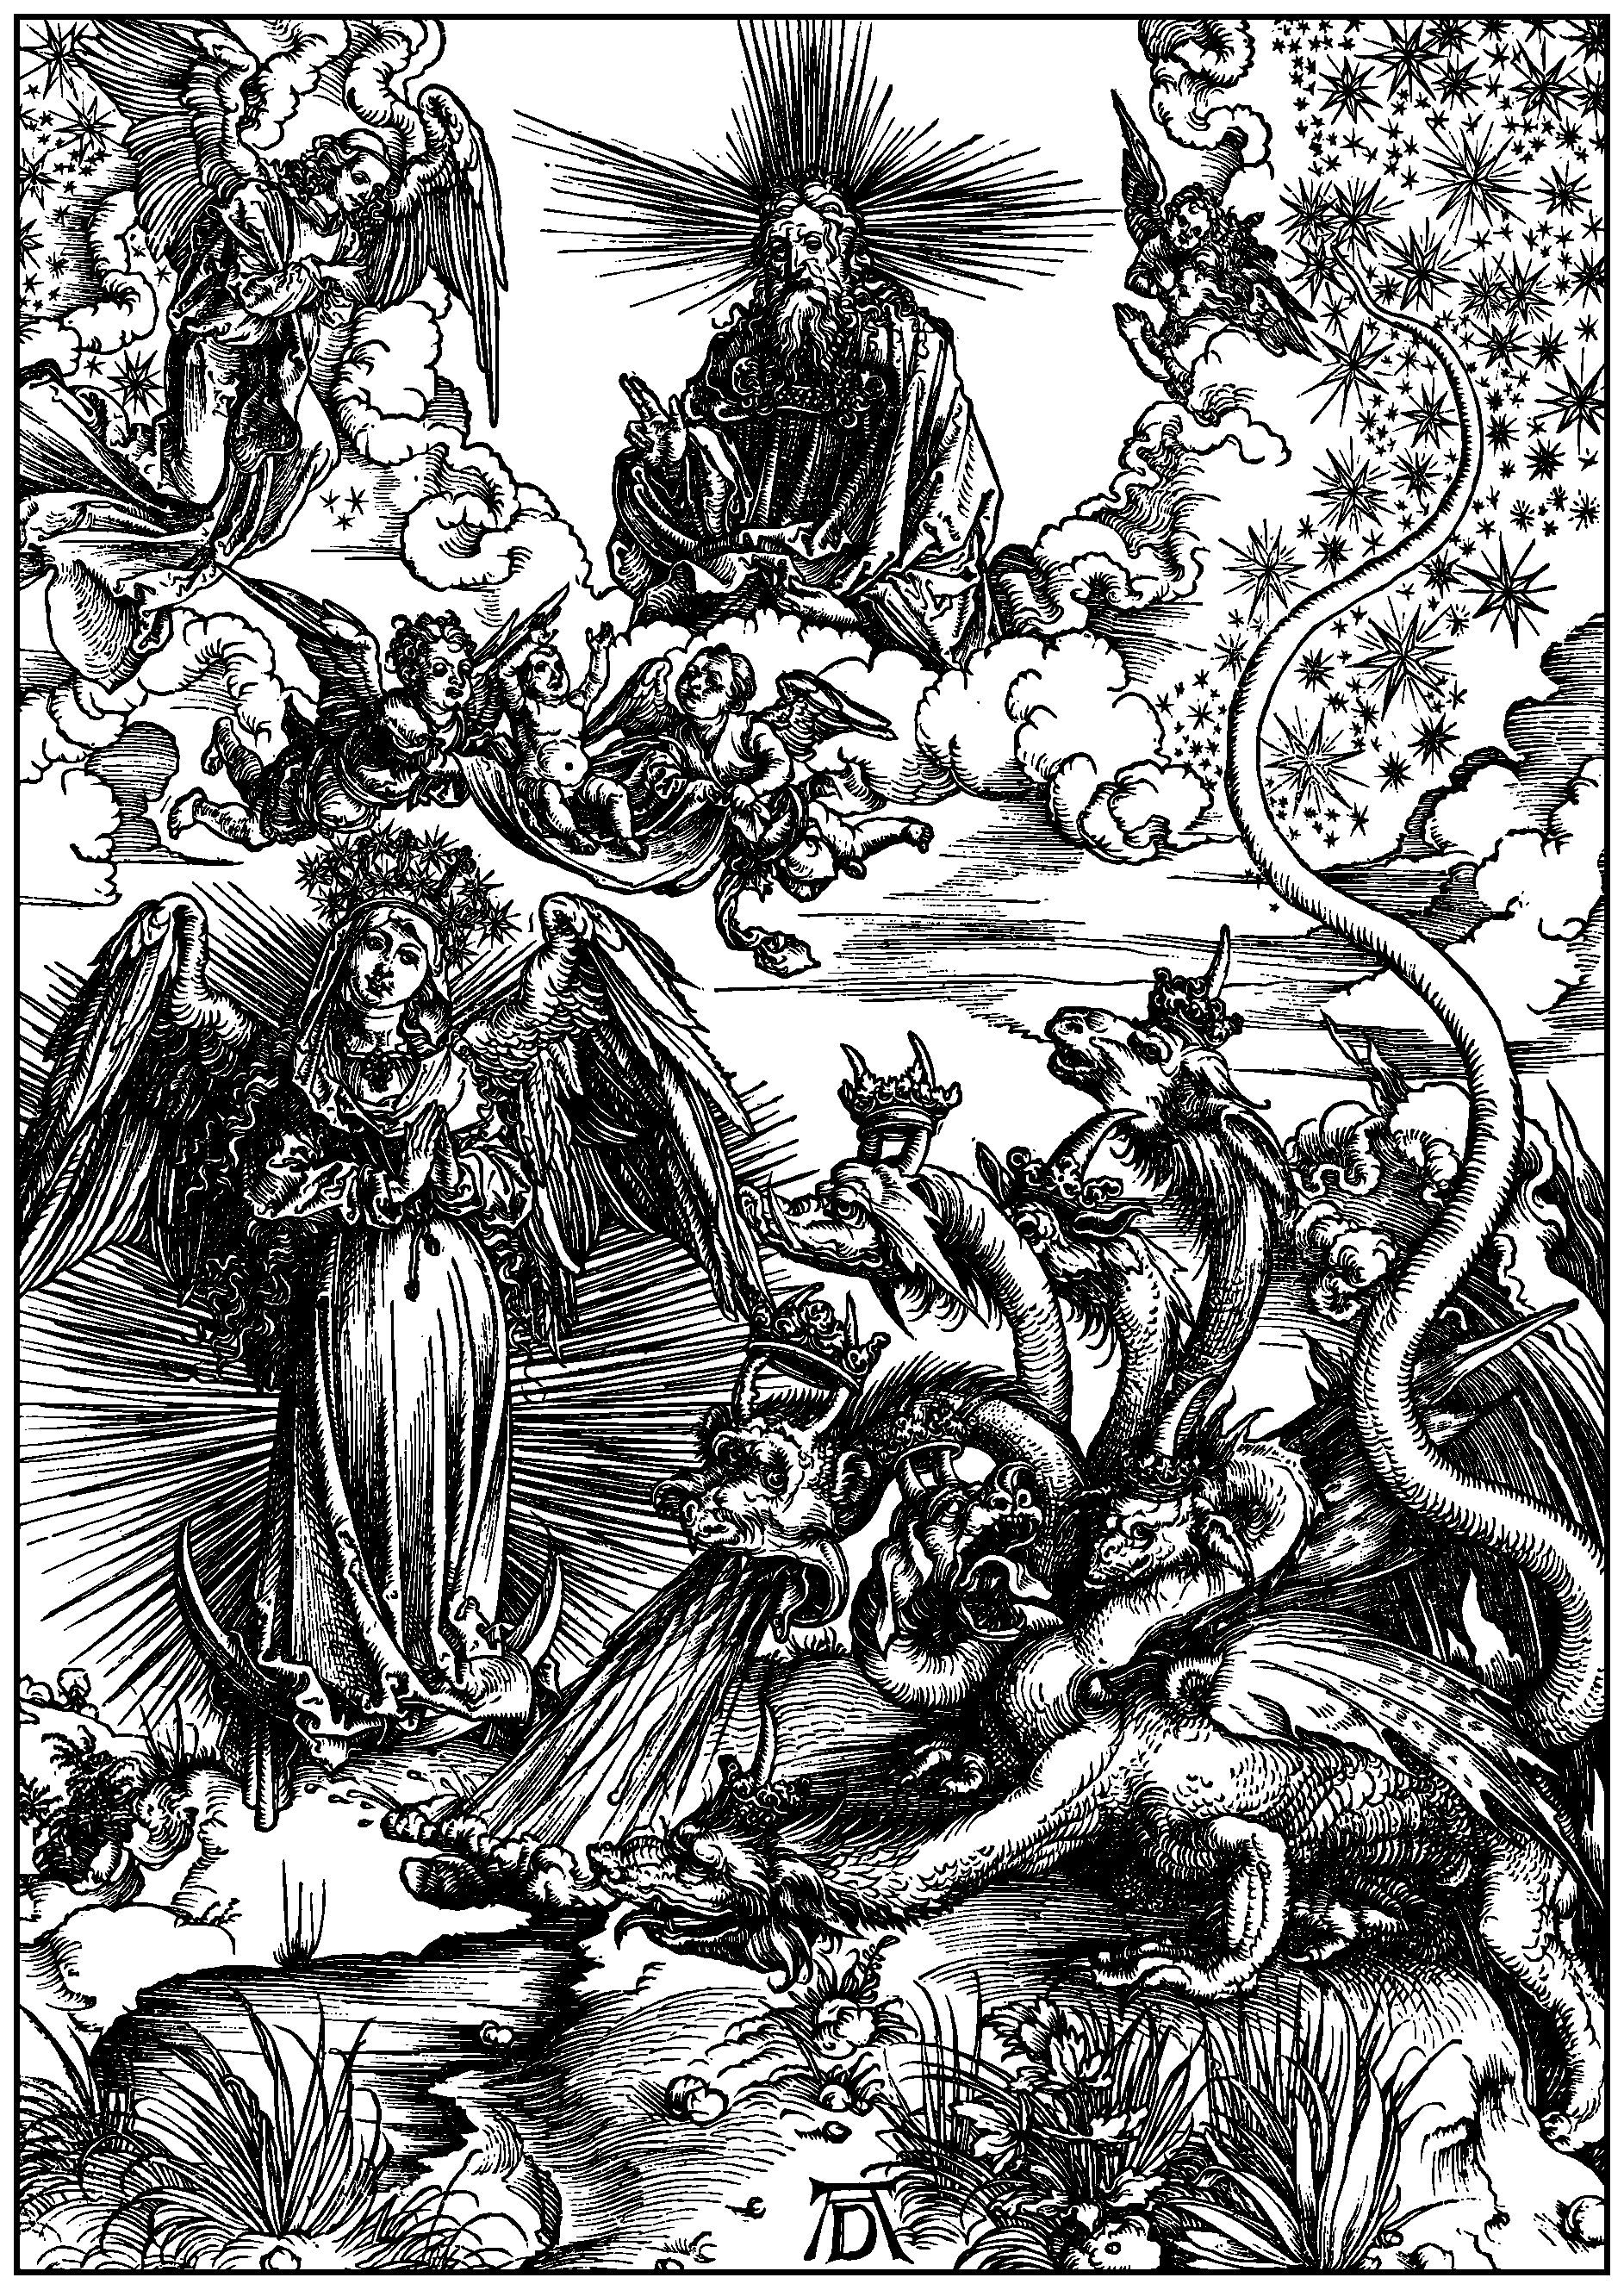
\includegraphics[width=103mm, height=145.935mm]{Propers/Sanctorum.eps}
    \caption{\textsc{\Huge{Proper of Saints}}}
\end{figure}
\fancyhead[C]{{\LARGE Proper of Saints}}
\fancyhead[RO,LE]{}
\fancyhead[RE,LO]{}
\phantomsection
\addcontentsline{toc}{section}{Through the Year}

\begin{rubric}
	Propers for Memorials are indicated by parentheses: ().
\end{rubric}

\begin{rubric}
	When a Common is specified, it is used for the propers, except for anything provided in the Feast Day itself.
	
	\textsc{Note,} Unless otherwise specified, the first options within a Common are used.
\end{rubric}

%A. Apostles
%Ab. Abbot
%E. Evangelist
%M. Martyr(ess)
%V. Virgin
%B. Bishop
%C. Confessor
%D. Doctor
%W. Widow
%Ma. Matron
%Em. Empress

\festival{Common Vigil}{29 November}{Vigil of St. Andrew}{A.}{LentenViolet}
\feastday{St. Andrew Vigil}
\feastdate{29}{November}

\lett{W}{e} beseech thee, Almighty God: that the blessed Apostle Andrew, whose festival we prevent, may implore thy help for us; that we, being absolved from our offences, may likewise be delivered from all dangers. Through.

\begin{rubric}
	Commemoration of the Feria (if it be Advent) \& \blackrubric{of St. Saturninus} (p. \pageref{SaturninusCollect}).
\end{rubric}


\subbymemorial{29 November}{St. Saturninus}{B.M.}{MartyrRed}
\feastday{{St. Saturninus}}
\feastdate{29}{November}

\memorialCollect\label{SaturninusCollect}
\lett{O}{God,} who vouchsafest unto us to rejoice in the birthday of thy blessed Martyr Saturninus: grant, we pray thee; that we may be succoured by his merits. Through.


\festival{Second Class Double}{30 November}{St. Andrew}{A.}{FestiveWhite}
\feastday{St. Andrew}
\feastdate{30}{November}

\begin{rubric}
	Common of Apostles (p. \pageref{CommonApostles}).
\end{rubric}

\openingSentence{The Lord loved Andrew in the odour of sweetness.}

%\begin{paracol}{2}[]
%\sloppy
\firstEvensong
\psalmAntiphon{Hail, precious Cross, {\dag} receive the disciple of him who hanged on thee, my Master Christ.}

\firstEvensongAntiphon{One of the two {\dag} which followed the Lord was Andrew, Simon Peter's brother, alleluia.}

%\switchcolumn

\mattins
\psalmAntiphon{Blessed Andrew {\dag} prayed saying: O Lord King of eternal glory, sustain me, as I hang upon the tree.}

\mattinsAntiphon{Yield up to us {\dag} a man so righteous, restore to us a man so holy: destroy not a man so dear to God, righteous, dutiful, and gentle.}

%\fussy
%\end{paracol}

\secondEvensong
\psalmAntiphon{Thou hast overwhelmed in hell, O Lord, {\dag} them that persecute the righteous: and thou wast leader on the wood of the Cross.}

\secondEvensongAntiphon{When blessed Andrew {\dag} came to the place where the Cross had been prepared, he cried out and said: O goodly Cross, so long desired, and now made ready for my eager spirit; fearless and joyful do I come to thee: therefore do thou also receive me gladly, as his disciple, who did hang upon thee.}

\collect
\lett{W}{e} humbly entreat thy Majesty, O Lord: that as blessed Andrew the Apostle was to thy Church a preacher and governor; so he may be a perpetual intercessor for us in thy sight. Through.

\begin{rubric}
    In Advent, Commemoration of the Feria.
\end{rubric}


\festival{Double (m.t.v.)}{2 December}{St. Peter Chrysologus}{B.C.D.}{FestiveWhite}
\feastday{{St. Peter Chrysologus}}
\feastdate{2}{December}

\begin{rubric}
	Common of a Confessor Bishop (p. \pageref{CommonConfessorBishop}).
\end{rubric}

\lett{O}{God,} who by divine foreshewing wast pleased to choose blessed Peter Chrysologus thy illustrious Doctor to rule and instruct thy Church: grant, we beseech thee; that, as we have had him for a Doctor of life on earth, so we may be found worthy to have him for an intercessor in heaven. Through.

\begin{rubric}
	Commemoration \blackrubric{of St. Bibiana} \& of the Advent Feria.
\end{rubric}


\subbymemorial{2 December}{St. Bibiana}{V.M.}{MartyrRed}
\feastday{{St. Bibiana}}
\feastdate{2}{December}

\memorialCollect
\lett{O}{God,} the giver of all good gifts, who in thy handmaid Bibiana didst unite the palm of martyrdom with the flower of virginity: unite by her intercession our hearts in charity with thee; that all perils being done away, we may attain unto everlasting rewards. Through.


\subbymemorial{4 December}{St. Barbara}{V.M.}{MartyrRed}
\feastday{{St. Barbara}}
\feastdate{4}{December}

\begin{rubric}
	Common of Virgins (p. \pageref{VirginMartyressCollect}).
\end{rubric}


%MANUAL ADJUSTMENT:
\clearpage
\subbymemorial{5 December}{St. Sabbas of Jud{\ae}a}{Ab.}{FestiveWhite}
\feastday{{St. Sabbas}}
\feastdate{5}{December}

\begin{rubric}
	Common of a Confessor not a Bishop (p. \pageref{AbbotCollect}).
\end{rubric}


\festival{Double}{6 December}{St. Nicholas}{B.C.}{FestiveWhite}
\feastday{{St. Nicholas}}
\feastdate{6}{December}

\begin{rubric}
	Common of a Confessor Bishop (p. \pageref{CommonConfessorBishop}).
\end{rubric}

\lett{O}{God,} who didst adorn thy blessed Bishop Nicholas with innumerable miracles: grant, we beseech thee; that by his merits and prayers we may be delivered from the fires of hell. Through.


\festival{Greater Double (m.t.v.)}{7 December}{St. Ambrose}{B.C.D.}{FestiveWhite}
\feastday{{St. Ambrose}}
\feastdate{7}{December}

\begin{rubric}
	Common of a Confessor Bishop (p. \pageref{CommonConfessorBishop}).
\end{rubric}

\lett{O}{God,} who didst give blessed Ambrose unto thy people to be a minister of everlasting salvation: grant, we beseech thee; that as we have learned of him the doctrine of life on earth, so we may be found worthy to have him for our advocate in heaven. Through.

\begin{rubric}
	Commemoration of the Advent Feria.
\end{rubric}


\festivalLL{Second Class Double with a Common Octave}{8 December}{Conception of the Blessed Virgin Mary}\label{ConceptionBVM}
\feastday{Conception B.V.M.}
\feastdate{8}{December}

\begin{rubric}
	Common of the Blessed Virgin Mary (p. \pageref{CommonBVM}).
\end{rubric}

\begin{paracol}{2}[]
\sloppy

\firstEvensong
\psalmAntiphon{Thou art all fair, O Mary; {\dag} there is no spot in thee.}\\

℣. To-day is the Conception of the holy Virgin Mary.

℟. Whose glorious life illumineth all the churches.

\firstEvensongAntiphon{All generations {\dag} shall call me blessed: for he that is mighty hath magnified me, alleluia.}

\switchcolumn

\mattins
\psalmAntiphon{Thou art the exaltation of Jerusalem, {\dag} thou art the glory of Israel, thou art the great rejoicing of our nation.}\\

℣. To-day is the Conception of the holy Virgin Mary.

℟. Whose glorious life illumineth all the churches.

\properantiphon{Ben.}{The Lord God said {\dag} unto the serpent, I will put enmity between thee and the woman, and between thy seed and her seed; it shall bruise thy head, alleluia.}

\fussy	
\end{paracol}

\secondEvensong
\psalmAntiphon{Blessed art thou, {\dag} O Virgin Mary, of the Most High God, above all the women upon the earth.}\\

℣. To-day is the Conception of the holy Virgin Mary.

℟. Whose glorious life illumineth all the churches.

\secondEvensongAntiphon{Let us celebrate {\dag} the worshipful Conception of the blessed and glorious Virgin Mary, whose lowliness the Lord regarded when at the word of an Angel she conceived the world's Redeemer, alleluia.}


\collect
\lett{O}{God,} mercifully hear the supplication of thy servants; that we who are assembled together on the Conception of the Virgin Mother of God, may at her intercession be delivered by thee from the dangers which beset us. Through.
\begin{rubric}
    Commemoration of the Advent Feria.
\end{rubric}


\subbymemorial{10 December}{Pope St. Melchiades of Rome}{B.M.}{MartyrRed}
\feastday{{Pope St. Melchiades}}
\feastdate{10}{December}

\begin{rubric}
	Common of a Martyr (p. \pageref{CommonMartyrNotBishopCollect}).
\end{rubric}


\subbymemorial{11 December}{Pope St. Damasus of Rome}{B.C.}{FestiveWhite}
\feastday{{Pope St. Damasus}}
\feastdate{11}{December}

\memorialCollect
\lett{G}{raciously} hear our prayers, O Lord: and at the intercession of blessed Damasus, thy Confessor and Bishop, mercifully grant us pardon and peace. Through.

\lettspace

\begin{rubric}
	Commemoration of the Octave \& Advent Feria.
\end{rubric}


%MANUAL ADJUSTMENT:
\clearpage
\festival{Greater Double}{13 December}{St. Lucy}{V.M.}{MartyrRed}
\feastday{{St. Lucy}}
\feastdate{13}{December}

\begin{rubric}
	Common of Virgins (p. \pageref{CommonVirgin}).
\end{rubric}


\begin{paracol}{2}[]
\sloppy

\firstEvensong
\psalmAntiphon{While holy Lucy {\dag} prayed, there appeared unto her the blessed Agatha, who consoled the handmaid of Christ.}\\

\firstEvensongAntiphon{In thy patience {\dag} thou didst possess thy soul, O Lucy, spouse of Christ: thou didst hate the things which are in the world, and thou shinest among the Angels: resisting unto blood, thou didst vanquish the enemy.}

\switchcolumn

\mattins
\psalmAntiphon{Through thee, O Virgin Lucy, {\dag} the Syracusan city shall be glorified by the Lord Jesus Christ.}\\

\mattinsAntiphon{A pillar art thou {\dag} that may not be moved, O Lucy, spouse of Christ: and all the people are waiting until thou receive the crown of life, alleluia.}

\end{paracol}

\secondEvensong
\psalmAntiphon{I bless thee, {\dag} O Father of my Lord Jesus Christ: for by thy Son the fire is quenched round about thine handmaid.}\\

℣. Full of grace are thy lips.

℟. Because God hath blessed thee for ever.

\secondEvensongAntiphon{With such gravity {\dag} was she endued by the Holy Spirit, that the virgin of the Lord remained unmoved.}

\collect
\lett{G}{raciously} hear us, O God of our salvation: that, like as we do rejoice in the festival of blessed Lucy thy Virgin; so we may be instructed in all godly and devout affection. Through.

\begin{rubric}
	Commemoration \blackrubric{of St. Herman of Alaska} from the Common of a Confessor not a Bishop (p. \pageref{ConfessorNotBishopCollect}), the Octave, \& the Advent Feria.
\end{rubric}


\subbymemorial{13 December}{St. Herman of Alaska (m.t.v.)}{C.}{FestiveWhite}
\feastday{{St. Herman}}
\feastdate{13}{December}

\begin{rubric}
	Common of a Confessor not a Bishop (p. \pageref{ConfessorNotBishopCollect}).
\end{rubric}


%MANUAL ADJUSTMENT:
\clearpage
\festivalLL{Semidouble}{14 December}{Day VII within the Octave of the Conception}
\feastday{{Conception Octave}}
\feastdate{14}{December}

\begin{rubric}
	Of the Octave, as on 9 December. But if Ember Wednesday fall on this day, of the Ember Day, with a Commemoration of the Octave.
\end{rubric}

%\begin{rubric}
%	If an Ember Day occur on any of the following Feasts, the Commemoration of the Feria is omitted.
%\end{rubric}


\festivalLL{Greater Double}{15 December}{Octave Day of the Conception of the Blessed Virgin Mary}
\feastday{{Conception Octave Day}}
\feastdate{15}{December}

\begin{rubric}
	As on the Feast (p. \pageref{ConceptionBVM}), Commemoration of the Advent Feria.
\end{rubric}


\subbymemorial{16 December}{St. Eusebius of Vercelli}{B.M.}{MartyrRed}
\feastday{{St. Eusebius}}
\feastdate{16}{December}

\begin{rubric}
	Common of a Martyr (p. \pageref{CommonMartyrBishopCollect}), second Collect.
\end{rubric}


\festivalLL{Greater Double}{18 December}{Expectation of the Blessed Virgin Mary}
\feastday{{Expectation B.V.M.}}
\feastdate{18}{December}

\begin{rubric}
	Common of the Blessed Virgin Mary (p. \pageref{CommonBVM}).
\end{rubric}

\openingSentence{Send ye the lamb to the ruler of the land from Sela to the wilderness, unto the mount of the daughter of Zion.\novr{Is. 16:1}}

%MANUAL ADJUSTMENT:
\vspace{-0.5\baselineskip}

\begin{paracol}{2}[]
\sloppy

\firstEvensong

\psalmAntiphon{Hail Mary, full of grace;~{\dag} The Lord is with thee; Blessed art thou amongst women. Alleluia.}\\

℣. Hail Mary, full of grace.

℟. The Lord is with thee.

\secondEvensong

\psalmAntiphon{The angel Gabriel was sent to the Virgin Mary, espoused to Joseph.}\\

℣. Hail Mary, full of grace.

℟. The Lord is with thee.

\switchcolumn

\mattins

\psalmAntiphon{Fear not, Mary:~{\dag} for thou hast found favour with God. Behold, thou shalt conceive in thy womb, and bring forth a son. Alleluia.}\\

℣. The Holy Ghost shall come upon thee.

℟. And the power of the Highest shall overshadow thee.

\antiphon{Ben.}{He shall sit upon the throne of David, {\dag} and of his kingdom, for ever.}

\fussy
\end{paracol}


\collect
\lett{O}{God,} who wast pleased that thy Word should take flesh of the womb of the Blessed Virgin Mary at the message of an Angel: grant to thy humble servants; that we who believe her to be truly the Mother of God may be aided by her intercession in thy sight. Through the same.


\festival{Vigil}{20 December}{Vigil of St. Thomas}{A.}{LentenViolet}
\feastday{{St. Thomas Vigil}}
\feastdate{20}{December}

%\begin{rubric}
%	If today be Sunday, in the Ember Saturday Mass, Commemoration is made of the anticipated Vigil of St. Thomas and the last Gospel of the Vigil is read at the end, the \nth{3} Collect is \blackrubric{of St. Mary in Advent} (p. \pageref{SPMaryInAdvent}).
%\end{rubric}

\begin{rubric}
	Common of Vigils of the Apostles (p. \pageref{CommonVigilApostles}), Commemoration of the Advent Feria.
\end{rubric}


\festival{Second Class Double}{21 December}{St. Thomas}{A.}{FestiveWhite}
\feastday{St. Thomas}
\feastdate{21}{December}

\begin{rubric}
	Common of Apostles (p. \pageref{CommonApostles}).
\end{rubric}

\properantiphon{Mag. \& Ben.}{Because thou hast seen me, {\dag} Thomas, thou hast believed: blessed are they that have not seen, and yet have believed, alleluia.}

\collect
\lett{G}{rant} us, we beseech thee, O Lord, to glory in the solemnity of thy blessed Apostle Thomas: that we may ever be succoured by his protection; and follow his faith with worthy devotion. Through.

\begin{rubric}
    Commemoration of the Advent Feria.
\end{rubric}


\subbymemorial{10 January}{St. Paul the First Hermit}{C.}{FestiveWhite}
\feastday{{St. Paul Hermit}}
\feastdate{10}{January}

\memorialCollect
\lett{O}{God,} who makest us glad with the yearly solemnity of blessed Paul, thy Confessor: mercifully grant; that, as we now celebrate his birthday, so we may follow the example of his life. Through.


\subbymemorial{11 January}{Pope St. Hyginus of Rome}{B.M.}{MartyrRed}
\feastday{{Pope St. Hyginus Rome}}
\feastdate{11}{January}

\begin{rubric}
	Common of a Martyr (p. \pageref{CommonMartyrBishopCollect}).
\end{rubric}


%MANUAL ADJUSTMENT:
\clearpage
\subbymemorial{12 January}{St. Benedict Biscop}{Ab.}{FestiveWhite}
\feastday{{St. Benedict Biscop}}
\feastdate{12}{January}

\memorialCollect
\lett{O}{God,} by whose gift the blessed Abbot Benedict left all things that he might be made perfect: grant unto all those who have entered upon the path of evangelical perfection, that they may neither look back nor linger in the way; but hastening to thee without stumbling, may lay hold upon eternal life. Through.


\festival{Double}{14 January}{St. Hilary}{B.C.D.}{FestiveWhite}
\feastday{{St. Hilary}}
\feastdate{14}{January}

\begin{rubric}
	Common of a Confessor Bishop (p. \pageref{CommonConfessorBishop}).
\end{rubric}

\begin{rubric}
	\textsc{Note,} Commemoration \blackrubric{of St. Felix} (p. \pageref{FelixCollect}).
\end{rubric}


\subbymemorial{14 January}{St. Felix of Nola}{M.}{MartyrRed}
\feastday{{St. Felix Nola}}
\feastdate{14}{January}

%\begin{rubric}
%	The Common of a Martyr (p. \pageref{CommonMartyr}).\par
%\end{rubric}

\memorialCollect\label{FelixCollect}
\lett{G}{rant,} we beseech thee, Almighty God, that the examples of thy Saints may provoke us to a better life: that as we celebrate their festival so we may imitate their actions. Through.


\festival{Greater Double}{15 January}{St. Maurus}{Ab.}{FestiveWhite}
\feastday{{St. Maurus}}
\feastdate{15}{January}

\begin{paracol}{2}[]
\sloppy

%MANUAL:
\vspace{-1\baselineskip}

\firstEvensong

\psalmAntiphon{The blessed Maurus, {\dag} born of a renowned and noble house, from his boyhood esteemed the reproach of Christ greater riches than the treasures of the world.}

\firstEvensongHymn\label{MaurusEvensong}

\hymnLett{D}{efender,} leader true, thine own companions deem'd

\hymnSecondLine{Thy splendour half divine, since all were less esteem'd:}

\begin{hangparas}{1.25em}{1}
For thy most worthy deeds, Maurus, accept the lays

Wherewith we celebrate thy praise.\\

Born of a noble stock, great honour was his due,

But palaces he spurn'd, and from the world withdrew;

Delights he trampl'd down, estates and robes unpric'd,

To undergo the yoke of Christ.\\

The holy Abbot's grace, before his eyes display'd,

By deeds of equal worth he eagerly portray'd;

The pattern of the life monastic shone in truth

From every action of the youth.\\

Sternly, with sackcloth rough, self-mastery he wrought,

And by the curb of law, unbroken silence sought;

The ever-watchful nights in fervent prayer he spent;

Whole days of fasting underwent\\

Right speedily he flew to do the father's hest,

Dry-shod, the waters deep with fearless feet he press'd;

And safely he return'd with Placidus, set free

Like Peter walking on the sea.\\

To thee, O Trinity, high praise and honour be,

Whose countenance desir'd the heaven-dwellers see:

Grant that the Holy Rule may be our pathway plain

The prize of Maurus to attain.  Amen.\\
\end{hangparas}

	℣. The Lord loved him and adorned him.

	℟. He clothed him with a robe of glory.
	
	\antiphon{Mag.}{O most blessed of men! {\dag} who, rejecting this world, bore the yoke of Holy Rule from tender years so lovingly; and being made obedient even unto death, he denied himself, that he might wholly cling to Christ his Master, alleluia.}
	
	\switchcolumn

%MANUAL:
\vspace{-1\baselineskip}

\mattins

\psalmAntiphon{Upheld by wings of obedience, {\dag} he walked upon the waters; and borne by the Spirit of God, he was saved from sinking in the flood.}

\mattinsInvitatoryHymn\label{MaurusInvitatory}
\hymnLett{I}{n} childhood Placidus was by his father giv'n;

\hymnSecondLine{Thus offer'd, he himself did freely yield to God.}

\begin{hangparas}{1.25em}{1}
Since first he came, he ever shone with wondrous grace,

A pattern to all zealous souls.\\

His Abbot sent him forth to fill an earthen crock,

He dips it in the lake, unwary, slips and falls,

A wave then carries him a bow-shot from the shore,

Out in the deep drowning is nigh.\\

But Maurus, what is this, that hast'ning to the lake,

Thou runnest o'er the waves as though thou wast on land?

Wont to obey, `tis thus thy holy father's voice

Doth lead thee to a miracle.\\

Straightway the lake restores Placidus safe again,

But whose the merit? Did his Nursian father draw

Him from the swirling depths, or was it Maurus' act?

The child resolves their questioning.\\

O Holy Trinity, through prayers of Placidus,

Grant to thy monks that by the narrow path of Rule

They may at length attain unto the courts of heav'n,

And mingle with celestial choirs. Amen.\\
\end{hangparas}

\mattinsOfficeHymn

\begin{rubric}
	Common of a Confessor not a Bishop (p. \pageref{CommonConfessorNotBishop}), the Versicle \& Antiphon of I Evensong.
\end{rubric}

\secondEvensong

\psalmAntiphon{He was chosen {\dag} by the Lord to be an example to the cloistered, and a chief observer of the Holy Rule.}

\secondEvensongHymn

\begin{rubric}
	Office Hymn of I Evensong.
\end{rubric}

℣. The Lord guided the righteous in right paths.

℟. And shewed him the kingdom of God.

\antiphon{Mag.}{To-day holy Maurus, {\dag} lying upon a goat-skin, died happily before the altar; to-day the first-begotten disciple of blessed Benedict, through the guiding of the Holy Rule, came up to Christ, rising untroubled, accompanied by choirs of Angels; today the obedient man, telling his victories, was worthy to be crowned by the Lord, alleluia.}

\fussy
\end{paracol}

\collect
\lett{O}{God,} who for a pattern of obedience didst cause blessed Maurus to walk dry-shod upon the waters: grant that we may both follow perfectly the example of his virtues, and also be worthy to share in his reward. Through.


\subbymemorial{16 January}{Pope St. Marcellus I of Rome}{B.M.}{MartyrRed}
\feastday{{Pope St. Marcellus I Rome}}
\feastdate{16}{January}

\memorialCollect
\lett{O}{Lord,} we beseech thee favourably to hear the prayers of thy people: that, as we do rejoice in the passion of blessed Marcellus thy Martyr and Bishop, so we may be succoured by his merits. Through.


\festival{Double}{17 January}{St. Anthony}{Ab.}{FestiveWhite}
\feastday{{St. Anthony}}
\feastdate{17}{January}

\begin{rubric}
	Common of a Confessor not a Bishop (p. \pageref{AbbotCollect}).
\end{rubric}


%MANUAL ADJUSTMENT:
\clearpage
\festival{Greater Double}{18 January}{Chair of St. Peter at Rome}{A.}{FestiveWhite}
\feastday{{Chair St. Peter Rome}}
\feastdate{18}{January}

\begin{rubric}
	As in the Feast of the Chair of St. Peter at Antioch (p. \pageref{CathedraAntioch}).
\end{rubric}

%\collect
\lett{O}{God,} who didst bestow upon thy blessed Apostle Peter the keys of the kingdom of heaven, and didst appoint unto him the high priesthood of binding and loosing: vouchsafe; that by the help of his intercession we may be delivered from the bonds of our iniquities. Who livest and reignest.

\lett{O}{God,} who by the preaching of the blessed Apostle Paul didst teach the multitude of the Gentiles: grant to us, we beseech thee; that we who celebrate his commemoration may know him to be our advocate with thee. (Through.)

\begin{rubric}
    Commemoration \blackrubric{of St. Prisca of Rome} (p. \pageref{PriscaCollect}).
\end{rubric}


\subbymemorial{18 January}{St. Prisca of Rome}{V.M.}{MartyrRed}
\feastday{{St. Prisca Rome}}
\feastdate{18}{January}

%\begin{rubric}
%	The Common of Virgins (p. \pageref{CommonVirgin}).
%\end{rubric}

\memorialCollect\label{PriscaCollect}
\lett{G}{rant,} we beseech thee, Almighty God: that we who celebrate the heavenly birthday of blessed Prisca, thy Virgin and Martyress; may both rejoice in her yearly solemnity, and profit by the example of so great a faith. Through.


\subbymemorial{19 January}{Sts. Marius, Martha, Audifax, \& Abachum}{M.}{MartyrRed}
\feastday{{Sts. Marius \&c.}}
\feastdate{19}{January}

\memorialCollect
\lett{G}{raciously} hear thy people, O Lord, who call upon thee with the advocacy of thy Saints: and grant us both to rejoice in peace in this temporal life; and to find succour unto life everlasting. Through.

\begin{rubric}
    Commemoration \blackrubric{of St. Mark of Ephesus} (p. \pageref{EphesianCollect}).
\end{rubric}


%PROVISIONAL:
\subbymemorial{19 January}{St. Mark of Ephesus (m.t.v.)}{B.C.}{FestiveWhite}
\feastday{{St. Mark Ephesus}}
\feastdate{19}{January}

%\begin{rubric}
%	The Common of a Confessor Bishop (p. \pageref{CommonConfessorBishop}), second Collect.
%\end{rubric}
%
%\par\noindent
%\textit{Yet to be approved.}
%
%\vspace{-1ex}
%
%\begin{tcolorbox}[
%  colback=white,           % background color
%  colframe=black,          % frame color
%  fonttitle=\itshape,     % optional font for title
%  title style={left=2mm},  % optional title left alignment
%  attach title to upper={},
%  enhanced,
%  boxed title style={size=small,colframe=black!50!white,colback=white},
%]
%\collect
\memorialCollect\label{EphesianCollect}
\lett{O}{Lord} Jesu Christ, the only Shepherd and Bishop of our souls; we beseech thee to keep us in thy truth, preserve us by thy grace, and govern us according to thy loving-kindness. That as we imitate the good example of blessed Mark thy Confessor and Bishop, we may grow in love for thy Word and service of thy Church. Who with.
%\end{tcolorbox}


%MANUAL ADJUSTMENT:
\clearpage
\festival{Double}{20 January}{Sts. Bishop Fabian \& Sebastian}{M.}{MartyrRed}
\feastday{{Sts. Fabian \& Sebastian}}
\feastdate{20}{January}

\begin{rubric}
	Common of Many Martyrs (p. \pageref{CommonMartyrs}).
\end{rubric}

%\collect
\lett{A}{lmighty} God, mercifully look upon our infirmities: that whereas we are oppressed by the burden of our sins, the glorious intercession of thy blessed Martyrs Fabian and Sebastian may be our succour and defence. Through.


\festival{Greater Double}{21 January}{St. Agnes of Rome}{V.M.}{MartyrRed}
\feastday{{St. Agnes Rome}}
\feastdate{21}{January}

\begin{rubric}
	Common of Virgins (p. \pageref{CommonVirgin}).
\end{rubric}

\begin{paracol}{2}
	\sloppy
	
\firstEvensong
\psalmAntiphon{When Agnes entered {\dag} the place of shame, she found the Angel of the Lord ready beforehand.}\\

\firstEvensongAntiphon{Blessed Agnes, {\dag} in the midst of the flames, stretched out her hands and prayed: I call on thee, O Father transcendent, august, and dread; for by thy holy Son's protection I have escaped the threats of an impious tyrant, and passed unscathed through the foulness of fleshly pollution: and behold, I come to thee, whom I have loved, whom I have sought, whom I have alway desired.}

\switchcolumn

\secondEvensong
\psalmAntiphon{Rejoice with me {\dag} and be exceeding glad, because among all these I have taken a throne of glory.}\\

℣. Full of grace are thy lips.

℟. Because God hath blessed thee for ever.

\antiphon{Mag.}{While the blessed Agnes {\dag} was standing in the midst of the flames, she stretched out her hands, and prayed unto God: Almighty Lord, worthy of all adoration, fear, and worship: I bless thy holy Name, and I glorify thee for ever and ever.}

\fussy
\end{paracol}

\mattins
\psalmAntiphon{With his ring {\dag} hath my Lord Jesus Christ betrothed me, and as his bride hath he crowned me.}

\mattinsAntiphon{Lo, that which I desired, {\dag} now I see; that for which I hoped, I now possess; I am united in heaven unto him, whom on earth I loved with a perfect devotion.}

\collect
\lett{A}{lmighty} and everlasting God, who dost choose the weak things of the world to confound those things that are strong: mercifully grant; that we who keep the feast of blessed Agnes thy Virgin and Martyress may feel the succour of her intercession in thy sight. Through.


\subbymemorial{22 January}{Sts. Vincent \& Anastasius}{M.}{MartyrRed}
\feastday{{St. Vincent \& Anastasius}}
\feastdate{22}{January}

%New propers needed for addition of Anastasius

\begin{rubric}
	Common of Many Martyrs (p. \pageref{CommonMartyrsNotBishopsCollect}).
\end{rubric}


\subbymemorial{23 January}{St. Emerentiana}{V.M.}{MartyrRed}
\feastday{{St. Emerentiana}}
\feastdate{23}{January}

\begin{rubric}
	Common of Virgins (p. \pageref{VirginMartyressCollect}), second Collect.
\end{rubric}


\festival{Double}{24 January}{St. Timothy}{B.M.}{MartyrRed}
\feastday{{St. Timothy}}
\feastdate{24}{January}

\begin{rubric}
	Common of a Martyr (p. \pageref{CommonMartyrBishopCollect}).
\end{rubric}


\festival{Greater Double}{25 January}{Conversion of St. Paul}{A.}{FestiveWhite}
\feastday{Conversion of St. Paul}
\feastdate{25}{January}

\begin{paracol}{2}[]
\sloppy

\firstEvensong

\psalmAntiphon{I have planted, {\dag} Apollos watered, but God gave the increase, alleluia.}

\firstEvensongHymn\label{PaulEvensong}

\hymnLett{O}{by} thy doctrine, Paul, thou sage illustrious,

\hymnSecondLine{Guide us in virtue, raise our spirits heavenwards;}

\begin{hangparas}{1.25em}{1}

Till perfect knowledge stream on us abundantly,

And that which only is in part be done away.\\

2. Glory eternal to the blessed Trinity,

With laud and honour, virtue and supremacy,

Trinal yet Onely, reigning in his majesty

Both now and ever, through the ages infinite. Amen.\\
\end{hangparas}

℣. Thou art a chosen vessel, holy Apostle Paul.

℟. A preacher of the truth throughout all the world.

\properantiphon{Mag.}{Go forth, Ananias, {\dag} and enquire for Saul, for behold, he prayeth: for he is a chosen vessel unto me, to bear my Name before the Gentiles, and Kings, and the children of Israel.}

\switchcolumn

\mattins

\psalmAntiphon{Most gladly will I glory {\dag} in my infirmities, that the power of Christ may rest upon me.}

\begin{rubric}
	Invitatory Hymn of I Evensong.
\end{rubric}

\begin{rubric}
	Office Hymn of I Evensong from the Common of the Apostles (p. \pageref{ApostlesEvensong}).
\end{rubric}

℣. Thou art a chosen vessel, holy Apostle Paul.

℟. A preacher of the truth throughout all the world.

\properantiphon{Ben.}{Ye which have followed me {\dag} shall sit upon twelve thrones, judging the twelve tribes of Israel, saith the Lord.}

\secondEvensong

\psalmAntiphon{The grace of God {\dag} which was bestowed upon me was not in vain: but his grace abideth with me always.}

\begin{rubric}
	The Office Hymn \& Versicle of I Evensong.
\end{rubric}

\properantiphon{Mag.}{O holy Apostle Paul, {\dag} thou preacher of the truth and Doctor of the Gentiles, intercede for us unto God, who hath chosen thee.}

\fussy
\end{paracol}

\collect
\lett{O}{God,} who, through the preaching of the blessed Apostle Saint Paul, hast caused the light of the Gospel to shine throughout the world; Grant, we beseech thee, that we, having his wonderful conversion in remembrance, may show forth our thankfulness unto thee for the same, by following the holy doctrine which he taught. Through.

\lett{O}{God,} who didst bestow upon thy blessed Apostle Peter the keys of the kingdom of heaven, and didst appoint unto him the high priesthood of binding and loosing: vouchsafe; that by the help of his intercession we may be delivered from the bonds of our iniquities. Who livest.


\subbymemorial{26 January}{St. Polycarp of Smyrna}{B.M.}{MartyrRed}
\feastday{{St. Polycarp Smyrna}}
\feastdate{26}{January}

\memorialCollect
\lett{O}{God,} who makest us glad with the yearly solemnity of blessed Polycarp, thy Martyr and Bishop: mercifully grant; that, as we now cebrate his birthday, so we may likewise rejoice in his protection. Through.


%MANUAL ADJUSTMENT:
\clearpage
\festival{Double (m.t.v.)}{27 January}{St. John Chrysostom}{B.C.D.}{FestiveWhite}
\feastday{{St. John Chrysostom}}
\feastdate{27}{January}

\begin{rubric}
	Common of a Confessor Bishop (p. \pageref{CommonConfessorBishop}).
\end{rubric}

%\collect
\lett{M}{ultiply,} we beseech thee, O Lord, thy Church with thy heavenly grace: even as thou didst vouchsafe to enlighten her with the glorious merits and doctrine of blessed John Chrysostom, thy Confessor and Bishop. Through.


%MANUAL ADJUSTMENT:
\vspace{-0.25\baselineskip}

\festival{Double}{28 January}{St. Cyril of Alexandria}{B.C.D.}{FestiveWhite}
\feastday{{St. Cyril Alexandria}}
\feastdate{28}{January}

\begin{rubric}
	Common of a Confessor Bishop (p. \pageref{CommonConfessorBishop}).
\end{rubric}

%\collect
\lett{O}{God,} who didst make blessed Cyril, thy Confessor and Bishop, an invincible defender of the divine Motherhood of the most blessed Virgin Mary: grant, by his intercession; that we, who believe her to be indeed the Mother of God, may be saved through her maternal protection. Through the same.

\begin{rubric}
    Commemoration \blackrubric{of St. Agnes} (p. \pageref{AgnesCollectII}).
\end{rubric}


%MANUAL ADJUSTMENT:
\vspace{-0.25\baselineskip}

\subbymemorial{28 January}{St. Agnes of Rome}{V.M.}{MartyrRed}
\feastday{{St. Agnes of Rome}}
\feastdate{28}{January}

\memorialCollect\label{AgnesCollectII}
\lett{O}{God,} who makest us glad with the yearly solemnity of blessed Agnes, thy Virgin and Martyress: grant, we beseech thee; that as we venerate her in our service, so we may follow the example of her godly conversation. Through.


%MANUAL ADJUSTMENT:
\vspace{-0.25\baselineskip}

\subbymemorial{30 January}{St. Martina}{V.M.}{MartyrRed}
\feastday{{St. Martina}}
\feastdate{30}{January}

\begin{rubric}
	Common of Virgins (p.\pageref{VirginMartyressCollect}).
\end{rubric}


%MANUAL ADJUSTMENT:
\vspace{-0.25\baselineskip}

\festival{Double}{1 February}{St. Ignatius of Antioch}{B.M.}{MartyrRed}
\feastday{{St. Ignatius Antioch}}
\feastdate{1}{February}

\begin{rubric}
	Common of a Martyr (p. \pageref{CommonMartyr}).
\end{rubric}

%\collect
\lett{A}{lmighty} God, mercifully look upon our infirmities; that whereas we are oppressed by the burden of our sins, the glorious intercession of blessed Ignatius thy Martyr and Bishop may be our succour and defence. Through.

\begin{rubric}
    Commemoration \blackrubric{of St. Bridget of Ireland} (p. \pageref{BridgetCollect}).
\end{rubric}


%MANUAL ADJUSTMENT:
\clearpage
\subbymemorial{1 February}{St. Bridget of Ireland}{V.}{FestiveWhite}
\feastday{{St. Bridget Ireland}}
\feastdate{1}{February}

%Sarum Propers:
%\begin{rubric}
%	The Common of Virgins (p. \pageref{CommonVirginOnlyII}.
%\end{rubric}

\memorialCollect\label{BridgetCollect}
\lett{W}{e} beseech thee, O Lord, that the prayers of Saint Bridget, thy Virgin, being pleasing unto thee, may help us: and never cease to entreat thy loving-kindness towards us. Through.


\festivalLL{Second Class Double}{2 February}{Purification of the Blessed Virgin Mary}
\feastday{Candlemas}
\feastdate{2}{February}

\begin{rubric}
	Common of the Blessed Virgin Mary (p. \pageref{CommonBVM}).
\end{rubric}

\openingSentence{It was revealed unto Simeon by the Holy Ghost, that he should not see death, before he had seen the Lord's Christ.}

\begin{paracol}{2}
\sloppy

\firstEvensong
\psalmAntiphon{When thou was born {\dag} ineffably of a Virgin, then were the Scriptures fulfilled: thou camest down like the rain into a fleece of wool, to bring salvation unto mankind: we praise thee, O our God.}\\

℣. It was revealed unto Simeon by the Holy Ghost. 

℟. That he should not see death before he had seen the Lord's Christ.

\firstEvensongAntiphon{The ancient {\dag} carried the Infant, but the Infant governed the ancient: he whom a Virgin bare, and after bearing, remained virgin, the same was worshipped by her who bare him.}

\switchcolumn

\mattins
\psalmAntiphon{Simeon, {\dag} a just and devout man, awaited the consolation of Israel; and the Holy Ghost was upon him.}

\mattinsAntiphon{And when the parents {\dag} brought in the Child Jesus, then Simeon took him up in his arms, and blessed God, saying: Lord, now lettest thou thy servant depart in peace.}

\secondEvensong
\psalmAntiphon{A light {\dag} to lighten the Gentiles, and the glory of thy people Israel.}

\secondEvensongAntiphon{To-day {\dag} the blessed Virgin Mary presented the Child Jesus in the temple; and Simeon, filled with the Holy Spirit, received him into his arms, and blessed God for ever.}

\fussy	
\end{paracol}

\collect
\lett{A}{lmighty} and everliving God, we humbly beseech thy Majesty, that, as thy only-begotten Son was this day presented in the temple in substance of our flesh, so we may be presented unto thee with pure and clean hearts. By the same thy Son Jesus Christ our Lord. Who liveth.


%MANUAL ADJUSTMENT:
\clearpage
\subbymemorial{3 February}{St. Blaise}{B.M.}{MartyrRed}
\feastday{{St. Blaise}}
\feastdate{3}{February}

\begin{rubric}
	Common of a Martyr (p. \pageref{CommonMartyrBishopCollect}), second Collect.
\end{rubric}


\subbymemorial{4 February}{St. Joseph of Aleppo}{M.}{MartyrRed}
\feastday{{St. Joseph Aleppo}}
\feastdate{4}{February}

\begin{rubric}
	Common of a Martyr (p. \pageref{CommonMartyrNotBishopCollect}).
\end{rubric}

\begin{rubric}
	Commemoration \blackrubric{of the New Martyrs of Russia,} from the Common of Many Martyrs (p. \pageref{CommonMartyrsNotBishopsCollect}).
\end{rubric}


\subbymemorial{4 February}{The New Martyrs of Russia}{M.}{MartyrRed}
\feastday{{New Russian Martyrs}}
\feastdate{4}{February}

\begin{rubric}
	Common of Many Martyrs (p. \pageref{CommonMartyrsNotBishopsCollect}).
\end{rubric}


\festival{Greater Double}{5 February}{St. Agatha}{V.M.}{MartyrRed}
\feastday{{St. Agatha}}
\feastdate{5}{February}

\begin{rubric}
	Common of Virgins (p. \pageref{CommonVirgin}).
\end{rubric}

%\begin{paracol}{2}
%\sloppy

\firstEvensong
\psalmAntiphon{Who art thou that comest unto me {\dag} to heal my wounds? I am the Apostle of Christ; be not doubtful of me, my daughter.}

\antiphon{Mag.}{The blessed Agatha, {\dag} standing in the midst of the prison, with outstretched hands entreated the Lord: O Lord Jesus Christ, my gracious Master, I give thanks unto thee, who hast enabled me to overcome the torments of the executioner: bid me now, O Lord, joyfully to enter into thine unfading glory.}

%\switchcolumn

\mattins
\psalmAntiphon{I give thee thanks, O Lord {\dag} Jesus Christ: because thou art mindful of me, and hast sent thine Apostle to heal my wounds.}

\antiphon{Ben.}{The multitude {\dag} of the heathen, fleeing to the tomb of the virgin, took thence her veil to defend them from the fire: that the Lord might shew himself a deliverer from the burning, for the merits of Agatha his blessed Martyr.}

%\fussy	
%\end{paracol}

\secondEvensong
\psalmAntiphon{On him who hath deigned {\dag} to heal me of all my wounds, and to restore my breast to my bosom; on him, the living God, do I call.}\\

℣. Full of grace are thy lips.

℟. Because God hath blessed thee for ever.

\antiphon{Mag.}{The blessed Agatha, {\dag} standing in the midst of the prison, with outstretched hands entreated the Lord: O Lord Jesus Christ, my gracious Master, I give thanks unto thee, who hast enabled me to overcome the torments of the executioner: bid me now, O Lord, joyfully to enter into thine unfading glory.}

\collect
\lett{O}{God,} who among the manifold works of thy power hast bestowed even upon the weakness of women the victory of martyrdom: mercifully grant; that we, who celebrate the birthday of blessed Agatha, thy Virgin and Martyress, may by her example be drawn nearer unto thee. Through.


\subbymemorial{6 February}{St. Dorothea}{V.M.}{MartyrRed}
\feastday{{St. Dorothea}}
\feastdate{6}{February}

%\begin{rubric}
%	The Common of Virgins (p. \pageref{CommonVirgin}.
%\end{rubric}

\memorialCollect
\lett{W}{e} beseech thee, O Lord, that as blessed Dorothea, thy Virgin and Martyress, was ever found pleasing unto thee, both by the merit of her chastity, and by her confession of thy power: so she may implore for us thy pardon. Through.


\subbymemorial{6 February}{St. Photius}{B.C.}{FestiveWhite}
\feastday{{St. Photius}}
\feastdate{6}{February}

\begin{rubric}
	Common of a Confessor Bishop (p. \pageref{ConfessorBishopCollect}).
\end{rubric}


\festival{Double (m.t.v.)}{7 February}{St. Romuald}{Ab.}{FestiveWhite}
\feastday{{St. Romuald}}
\feastdate{7}{February}

\begin{rubric}
	Common of a Confessor not a Bishop (p. \pageref{AbbotCollect}).
\end{rubric}


\subbymemorial{9 February}{St. Apollonia of Alexandria}{V.M.}{MartyrRed}
\feastday{{\small St. Apollonia Alexandria}}
\feastdate{9}{February}

%\begin{rubric}
%	The Common of Virgins (p. \pageref{CommonVirgin}.
%\end{rubric}

\memorialCollect
\lett{O}{God} who among the manifold works of thy power hast bestowed even upon the weakness of women the victory of martyrdom mercifully grant; that we, who celebrate the birthday of blessed Apollonia thy Virgin and Martyress, may by her example be drawn nearer unto thee. Through.


%MANUAL ADJUSTMENT:
\clearpage
\festival{Greater Double}{10 February}{St. Scholastica}{V.}{FestiveWhite}
\feastday{{St. Scholastica}}
\feastdate{10}{February}

\begin{paracol}{2}[]
\sloppy

%MANUAL ADJUSTMENT:
\vspace{-1\baselineskip}

\firstEvensong
\psalmAntiphon{Lo, I entreated thee, {\dag} and thou wouldest not hear me: I entreated my Lord, and he heard me.}

\firstEvensongHymn\label{ScholasticaEvensong}

\hymnLett{B}{lessed} bride of Christ the Bridegroom, Dove of virgins, holy maid,

\hymnSecondLine{Starry hosts proclaim thy praises, Praise the crown to virtue paid,}

\begin{hangparas}{1.25em}{1}

While our joyful hearts and voices Join the anthem unafraid.\\

2. Wise wert thou to spurn the riches And the crowns that heaven miss,

Wise to choose thy brother's teachings, Change thy way of life for his:

In the savour of thine ointments Didst thou enter heav'nly bliss.\\

3. Oh, the might of love unbounded! Victory of all most meet!

At thy tears the heavens opened, Poured their floods about thy feet,

While his soul to thine made answer All night long in converse sweet.\\

4. Crash of tempest, roll of thunder, Lightning flash from pole to pole,

But the storm of love is stronger, Brighter flashes in the soul,

While the peace of Christ the Bridegroom Holds thee still and keeps thee whole.\\

5. Now a gleaming cloud in heaven, Now a sun with golden rays,

Never darkling, never fading, Shining still through all our days,

Fill the hearts of all the faithful With the joy of heav'nly lays.\\

6. Glory to the Father sing we, Glory to the only Son;

To the Paraclete in glory, Equal tribute be begun,

At whose pleasure made and govern'd All the ages' course is run. Amen.\\
\end{hangparas}

℣. Who is this that flieth as a cloud? 

℟. And as a dove to her windows?

\antiphon{Mag.}{Let all the multitude {\dag} of the faithful exult in the glory of the gracious virgin Scholastica: and chiefly let the company of virgins be joyful, celebrating her Solemnity; for she besought the Lord, pouring forth her tears, and of him received greater power, because her love was greater.}

\secondEvensong
\psalmAntiphon{When holy Benedict {\dag} had withdrawn himself in his cell for three days, he lifted up his eyes, and saw the soul of his sister, departing from the body in the likeness of a dove, enter the secret places of the heavens.}\\

%MANUAL ADJUSTMENT:
\vspace{-1\baselineskip}

\begin{rubric}
	Office Hymn \& Versicle of I Evensong.
\end{rubric}

\antiphon{Mag.}{To-day {\dag} the holy virgin Scholastica, in the likeness of a dove, went forth with all gladness to the heavenly places: to-day she was found worthy to enjoy for ever the bliss of celestial life beside her brother.}

\collect
\lett{O}{God,} who didst reveal in a vision the soul of blessed Scholastica thy Virgin entering heaven in the likeness of a dove, that thou mightest shew the way of the undefiled: grant us by the aid of her merits and prayers so innocently to live, that we may worthily attain unto joys eternal. Through.

\switchcolumn

%MANUAL ADJUSTMENT:
\vspace{-1\baselineskip}

\mattins
\psalmAntiphon{Now speak we {\dag} even until morning of heavenly things, in holy converse regarding the life of the spirit.}

\mattinsInvitatoryHymn\label{ScholasticaInvitatory}

\hymnLett{N}{ow} we our voices raise in sweet angelic hymn,

\hymnSecondLine{While earthly hills and vales in silent night grow dim:}

\begin{hangparas}{1.25em}{1}

Scholastica calls forth a heav'nly melody

From souls of virgin purity.\\

2. She, sprung from Nursian race, her stem nobility,

As bride to Virgin Lamb more noble yet shall be;

The fragrance of the Spouse she ever doth impart,

The beauty of his wounded Heart.\\

3. At their fraternal meal besought she zealously:

For greater nourishment hunger'd her charity.

And so with still more joy her brother truth outpour'd

While she more fervently implor'd.\\

4. O peaceful hours of night, O time of quiet rest,

When heav'nly feasting so inebriates the breast,

While words of loving zeal from one another flow;

Thy will, O Jesus, they would know.\\

5. O very Rest of heart, O wondrous Trinity

Whose glance doth satiate with heav'nly radiancy,

May talk of thee be sweet, more sweet thee to attain,

Sweetest eternally to gain. Amen.
\end{hangparas}

\mattinsOfficeHymn\label{ScholasticaMattins}

\hymnLett{T}{he} shades of night are fled away,

\hymnSecondLine{The long desired day is born;}

\begin{hangparas}{1.25em}{1}

The changing wheel of time has brought

Scholastica her wedding morn.\\

2. The winter's weariness is past,

Tempests no longer doth she see;

The fields of heaven bloom with stars,

The blossoms of eternity.\\

3. He calls her forth, the Source of love,

He gives her wings that she may rise,

And to the kisses of his mouth,

A shining dove she swiftly flies.\\

4. O royal child, how fair thy course!

O maid, how beautiful thy way!

Thy brother marks thy upward flight,

Then turns to God his thanks to pay.\\

5. Lock'd in the Bridegroom's close embrace,

She takes the crown to virtue owed,

Sunk in a glorious stream of bliss,

Inebriated with her God.\\

6. Thou lily of the valley, Christ,

To thee our homage meet we pay:

To Father and to Paraclete,

While endless ages roll away. Amen.\\
\end{hangparas}

℣. Behold, thou art fair, my love.  

℟. Behold, thou art fair; thou hast dove's eyes.

\antiphon{Ben.}{O how illustrious {\dag} are the merits of blessed Scholastica! O how great the power of her tears! through which the renowned virgin, out of sunny clearness, drew down from the air a mighty flood of rain.}

\end{paracol}


\subbymemorial{11 February}{Pope St. Gregory II}{B.C.}{FestiveWhite}
\feastday{{Pope St. Gregory II}}
\feastdate{11}{February}

\begin{rubric}
	Common of a Confessor Bishop (p. \pageref{ConfessorBishopCollect}).
\end{rubric}


\subbymemorial{14 February}{St. Valentine}{M.}{MartyrRed}
\feastday{{St. Valentine}}
\feastdate{14}{February}

%\begin{rubric}
%	The Common of a Martyr (p. \pageref{CommonMartyr}).
%\end{rubric}

\memorialCollect
\lett{G}{rant,} we beseech thee, Almighty God: that we who observe the birthday of blessed Valentine thy Martyr may by his intercession be delivered from all evils that beset us. Through.


\subbymemorial{15 February}{Sts. Faustinus and Jovita}{M.}{MartyrRed}
\feastday{{Sts. Faustinus \& Jovita}}
\feastdate{15}{February}

%\begin{rubric}
%	The Common of Many Martyrs (p. \pageref{CommonMartyrs}).
%\end{rubric}

\memorialCollect
\lett{O}{God,} who makest us glad with the yearly solemnity of thy holy Martyrs Faustinus and Jovita: mercifully grant; that as we rejoice in their merits, so we may be enkindled by their example. Through.


\subbymemorial{18 February}{St. Simeon of Jerusalem}{B.M.}{MartyrRed}
\feastday{{St. Simeon Jerusalem}}
\feastdate{18}{February}

\begin{rubric}
	Common of a Martyr (p. \pageref{CommonMartyrBishopCollect}).
\end{rubric}


%MANUAL ADJUSTMENT:
\clearpage
\festival{Second Class Double}{22 February}{Chair of St. Peter at Antioch}{A.}{FestiveWhite}\label{CathedraAntioch}
\feastday{Chair St. Peter Antioch}
\feastdate{22}{February}


\begin{paracol}{2}
\sloppy

\firstEvensong\label{PeterAntiochEvensong}
\psalmAntiphon{Behold a great priest, {\dag} who in his days pleased God, and was found righteous.}

\firstEvensongHymn
\selectlanguage{ecclesiasticallatin}

%I fear I did a bad job translating, so I'm just supplying the Latin here.
\hymnLett{Q}{uodc\smash{ú}mque} vinclis super terram strínxeris,

\hymnSecondLine{Erit in astris religátum fórtiter:}
\begin{hangparas}{1.25em}{1}
Et quod resólvis in terris arbítrio,

Erit solútum super cæli rádium:

In fine mundi judex eris sǽculi.\\

2. Gloria Patriper imménsa sǽcula;

Sit tibi, Nate, decus et impérium;

Honor, potéstas, Sanctóque Spirítui:

Sit Trinitáti salus individua,

Per infiníta sæculórum sǽcula. Amen.\\
\end{hangparas}

\selectlanguage{british}
    
    ℣. Thou art Peter.

	℟. And upon this rock I will build my Church.
	
\firstEvensongAntiphon{Thou art the shepherd of the sheep, {\dag} Prince of the Apostles, unto thee were given the keys of the kingdom of heaven.}

\switchcolumn

\mattins
\psalmAntiphon{The Lord, {\dag} therefore, assured him by an oath that he would bless the nations in his seed.}

\begin{rubric}
	Invitatory Hymn of I Evensong.
\end{rubric}

\mattinsOfficeHymn\label{PeterAntiochMattins}

\hymnLett{P}{eter,} good shepherd, may thy ceaseless orisons,

\hymnSecondLine{For us prevailing, break the bands of wickedness:}
\begin{hangparas}{1.25em}{1}
For thou of old time didst receive authority

The gates to open, or to close, of Paradise.\\

2. Glory eternal to the blessed Trinity,

With laud and honour, virtue and supremacy,

Trinal yet Onely, reigning in his majesty

Both now and ever, through the ages infinite. Amen.\\
\end{hangparas}

    ℣. Thou art Peter.

	℟. And upon this rock I will build my Church.
	
	\properantiphon{Ben.}{Whatsoever {\dag} thou shalt bind on earth shall be bound in heaven: and whatsoever thou shalt loose on earth shall be loosed in heaven, saith the Lord unto Simon Peter.}

\fussy	
\end{paracol}

\secondEvensong
\psalmAntiphon{Good and faithful servant, {\dag} enter thou into the joy of thy Lord.}

\begin{rubric}
	Office Hymn \& Versicle of I Evensong.
\end{rubric}

\properantiphon{Mag.}{Whilst he was chief Bishop, he feared nothing on earth, but ascended gloriously to the heavenly kingdoms.}


\collect
\lett{O}{God,} who didst bestow upon thy blessed Apostle Peter the keys of the kingdom of heaven, and didst appoint unto him the high priesthood of binding and loosing: vouchsafe; that by the help of his intercession we may be delivered from the bonds of our iniquities. Who livest.

\lett{O}{God,} who by the preaching of the blessed Apostle Paul didst teach the multitude of the Gentiles: grant to us, we beseech thee; that we who celebrate his commemoration may know him to be our advocate with thee. (Through.)

\begin{rubric}
    If this Feast fall on a Saturday---not in a Leap Year---Commemoration is made \blackrubric{of the Vigil of St. Matthias,} from the Common of Vigils of the Apostles (p. \pageref{CommonVigilApostles}).
\end{rubric}

\begin{rubric}
    In Lent, Commemoration of the Feria.
\end{rubric}


\festival{Vigil}{23/24 February}{Vigil of St. Matthias}{A.}{LentenViolet}\label{MatthiasVigil}
\feastday{{St. Matthias Vigil}}
\feastdate{23/24}{February}

\begin{rubric}
	Common of Vigils of the Apostles (p. \pageref{CommonVigilApostles}).
\end{rubric}


\festival{Second Class Double}{24/25 February}{St. Matthias}{A.}{FestiveWhite}
\feastday{St. Matthias}
\feastdate{24/25}{February}

\begin{rubric}
	Common of Apostles (p. \pageref{CommonApostles}).
\end{rubric}

\lett{O}{God,} who didst join blessed Matthias to the college of thine Apostles: grant, we beseech thee; that through his mediation we may ever perceive thy tender mercy towards us. Through.
\begin{rubric}
    In Lent, Commemoration of the Feria.
\end{rubric}


%MANUAL ADJUSTMENT:
\clearpage
\subbymemorial{25/26 February}{St. Walburga of Heidenheim}{V.}{FestiveWhite}
\feastday{{St. Walburga Heidenheim}}
\feastdate{25/26}{February}

%\begin{rubric}
%	The Common of Virgins (p. \pageref{CommonVirgin}).
%\end{rubric}

\memorialCollect
\lett{O}{God,} who among the manifold gifts of thy grace dost also work great wonders even in the weaker sex: mercifully grant that we may feel the help of the intercession of blessed Walburga, thy Virgin, whose example of chastity doth enlighten us, and whose glory in miracles doth gladden us. Through.


\subbymemorial{26/27 February}{Pope St. Alexander of Alexandria}{B.C.}{FestiveWhite}
\feastday{{Pope St. Alexander}}
\feastdate{26/27}{February}

\begin{rubric}
	Common of a Confessor Bishop (p. \pageref{ConfessorBishopCollect}).
\end{rubric}


\festival{Greater Double}{27/28 February}{St. Raphael of Brooklyn}{B.C.}{FestiveWhite}
\feastday{{St. Raphael Brooklyn}}
\feastdate{27/28}{February}

\begin{rubric}
	In Lent, Commemoration only.
\end{rubric}

\begin{rubric}
	Common of a Confessor Bishop (p. \pageref{CommonConfessorBishop}).
\end{rubric}

%MANUAL ADJUSTMENT:
\lett{A}{lmighty}\textls[-15]{ God, who hast instructed thy Church with the heavenly doctrine of thy Bishop and Confessor Saint Raphael of Brooklyn; and hast provided in his life an example of the Good Shepherd who collects the lost sheep; grant us so to follow in his godly footsteps, that, ever helped by his intercession, we with him may attain to thy heavenly kingdom. Through the same.}


\subbymemorial{1 March}{St. David of Wales}{B.C.}{FestiveWhite}
\feastday{{St. David Wales}}
\feastdate{1}{March}

%\begin{rubric}
%	The Common of a Confessor Bishop (p. \pageref{CommonConfessorBishop}).
%\end{rubric}

\memorialCollect
\lett{G}{rant} to us, Almighty God: that the loving intercession of blessed David, thy Confessor and Bishop, may protect us; that while we celebrate his festival we may imitate his steadfastness in the defence of the Catholic faith. Through.


\subbymemorial{2 March}{St. Chad}{B.C.}{FestiveWhite}
\feastday{{St. Chad}}
\feastdate{2}{March}

%\begin{rubric}
%	The Common of a Confessor Bishop (p. \pageref{CommonConfessorBishop}).
%\end{rubric}

\memorialCollect
\lett{A}{lmighty} and everlasting God, who on this day dost gladden us by the festival of blessed Chad, thy Confessor and Bishop: we humbly beseech thy mercy; that we, who devoutly observe and venerate his festival, may by his loving advocacy obtain the reward of everlasting life. Through.


%MANUAL ADJUSTMENT:
\clearpage
\subbymemorial{4 March}{Pope St. Lucius I of Rome}{B.M.}{MartyrRed}
\feastday{{Pope St. Lucius I}}
\feastdate{4}{March}

%\begin{rubric}
%	The Common of a Martyr (p. \pageref{CommonMartyr}).
%\end{rubric}

\memorialCollect
\lett{O}{God,} who makest us glad with the yearly solemnity of blessed Lucius thy Martyr and Bishop: mercifully grant; that, as we now celebrate his birthday, so we may likewise rejoice in his protection. Through.


\festival{Double}{6 March}{Sts. Perpetua and Felicitas}{M.}{MartyrRed}
\feastday{{Sts. Perpetua \& Felicitas}}
\feastdate{6}{March}

\begin{rubric}
	In Lent, Commemoration only.
\end{rubric}

\begin{rubric}
	Common of Holy Matrons (p. \pageref{CommonHolyMatrons}).
\end{rubric}

\lett{G}{rant,} we beseech thee, O Lord our God, that we may at all times so devoutly honour the triumphs of thy holy Martyrs Perpetua and Felicitas: that, although we cannot worthily shew forth their praises, yet we may continually honour them with lowly service. Through.


\subbymemorial{9 March}{St. Gregory of Nyssa}{B.C.D.}{FestiveWhite}
\feastday{{St. Gregory Nyssa}}
\feastdate{9}{March}

\begin{rubric}
	Common of a Confessor Bishop (p. \pageref{ConfessorBishopDoctorCollect}).
\end{rubric}


\subbymemorial{10 March}{The Forty Holy Martyrs}{M.}{MartyrRed}
\feastday{{40 Holy Martyrs}}
\feastdate{10}{March}

\memorialCollect
\lett{G}{rant} we beseech thee, Almighty God: that, like as we have known thy glorious Martyrs to be constant in their confession, so we may perceive their loving intercession for us with thee. Through.


\festival{Second Class Double}{12 March}{Pope St. Gregory the Great}{B.C.D.}{FestiveWhite}
\feastday{Pope St. Gregory}
\feastdate{12}{March}

\begin{paracol}{2}
\sloppy

%MANUAL ADJUSTMENT:
\vspace{-1\baselineskip}

\firstEvensong\label{GregoryEvensong}
\psalmAntiphon{The blessed Gregory, {\dag} lifted up to the throne of Peter, shewed forth in deed his name of `the Watchful.'}

\firstEvensongHymn

\hymnLett{A}{postle} of the English, thou

\hymnSecondLine{Art comrade of the Angels now:}
\begin{hangparas}{1.25em}{1}
O help the faithful, Gregory,

Who heardest then the peoples' cry.\\

2. Abundant wealth was naught to thee

Who, seeking princely penury,

Didst spurn the glory of the earth

To follow Jesus in his dearth.\\

3. Like some poor needy shipwreck'd soul,

His messenger besought a dole;

Twin gifts thou gavest; nothing loth

To offer self and silver both.\\

4. First in his Church from that time forth

Christ set thee, in thy proven worth;

So didst thou rise to Peter's throne,

Whose life was pattern for thine own.\\

5. O Priest and Leader of the flock,

The Church's glory, light, and rock,

Instructed by thy wise command,

Let not the sheep in peril stand.\\

6. Praise to the unbegotten One,

And glory to his only Son;

And thine, O Spirit, Breath of God,

Be equal majesty and laud. Amen.\\
\end{hangparas}

    ℣. The Lord loved him and adorned him.

	℟. He clothed him with a robe of glory.

\firstEvensongAntiphon{O Teacher right excellent, {\dag} O light of Holy Church, O blessed Gregory, lover of the divine law: intercede for us unto the Son of God.}

\switchcolumn

%MANUAL ADJUSTMENT:
\vspace{-1\baselineskip}

\mattins\label{GregoryMattins}
\psalmAntiphon{While he revealed {\dag} the mysteries of Holy Writ, there appeared a dove, whiter than snow.}

\begin{rubric}
	Invitatory Hymn of I Evensong.
\end{rubric}

\mattinsOfficeHymn

\hymnLett{T}{hy} lips, O Gregory, distil

\hymnSecondLine{The honey that thy heart doth fill;}
\begin{hangparas}{1.25em}{1}

In spiced sweetness floweth thence

The savour of thine eloquence.\\

2. The hidden mysteries that lie

In Holy Scripture, to thine eye

Are plain; the Truth himself draws near

To make their subtle secrets clear.\\

3. At once the Apostolic throne

And majesty become thine own:

O free us from sin's binding chain

That heav'nly mansions we may gain.\\

4. O Priest and Leader of the flock,

The Church's glory, light, and rock,

Instructed by thy wise command,

Let not the sheep in peril stand.\\

5. Praise to the unbegotten One,

And glory to his only Son;

And thine, O Spirit, Breath of God,

Be equal majesty and laud. Amen.\\
\end{hangparas}

    ℣. The Lord guided the righteous in right paths.

	℟. And shewed him the kingdom of God.

\mattinsAntiphon{Gregory, {\dag} when he looked upon the youthful Angles, said: They have the countenance of Angels, and such as these should be of the fellowship of the Angels in heaven.}

\secondEvensong

\begin{rubric}
	Office Hymn \& Antiphon of I Evensong. Versicle of Mattins.
\end{rubric}

\fussy	
\end{paracol}


\collect
\lett{O}{God,} who on the soul of thy servant Gregory, hast bestowed the rewards of everlasting bliss: mercifully grant; that we, who are oppressed by the burden of our sins, may by his prayers before thee be relieved. Through.


\festival{Double}{17 March}{St. Patrick}{B.C.}{FestiveWhite}
\feastday{{St. Patrick}}
\feastdate{17}{March}

\begin{rubric}
	In Lent, Commemoration only.
\end{rubric}

\begin{rubric}
	Common of a Confessor Bishop (p. \pageref{CommonConfessorBishop}).
\end{rubric}

\lett{O}{God,} who for the preaching of thy glory unto the Gentiles wast pleased to send forth blessed Patrick, thy Confessor and Bishop: grant by his merits and intercession; that we may through thy mercy be enabled to accomplish those things which thou commandest us to do. Through.

\begin{rubric}
    Commemoration \blackrubric{of St. Joseph of Arimathea} (p. \pageref{ArimatheanCollect}).
\end{rubric}


\subbymemorial{17 March}{St. Joseph of Arimathea}{C.}{FestiveWhite}
\feastday{{St. Joseph Arimathea}}
\feastdate{17}{March}

%\begin{rubric}
%	The Common of a Confessor not a Bishop (p. \pageref{CommonConfessorNotBishop}).
%\end{rubric}

\memorialCollect\label{ArimatheanCollect}
\lett{O}{God,} who didst give such grace unto thy servant Joseph that he boldly craved the body of Jesus, and with great reverence laid him in the rock-hewn sepulchre: grant, we beseech thee, that we likewise may be so emboldened for thee, as to do works meet for thy Kingdom. Through the same.


\festival{Double}{18 March}{St. Cyril of Jerusalem}{B.C.D.}{FestiveWhite}
\feastday{{St. Cyril Jerusalem}}
\feastdate{18}{March}

\begin{rubric}
	In Lent, Commemoration only.
\end{rubric}

\begin{rubric}
	Common of a Confessor Bishop (p. \pageref{CommonConfessorBishop}).
\end{rubric}

\label{CyrilCollect}
\lett{G}{rant} to us, we beseech thee, Almighty God, at the intercession of the blessed Bishop Cyril: so to know thee, the only true God, and Jesus Christ whom thou hast sent; that we may be found worthy to be numbered for evermore among the sheep who hear his voice. Through the same.

\begin{rubric}
	Commemoration \blackrubric{of King St. Edward} (p. \pageref{EdwardCollect}).
\end{rubric}


%MANUAL ADJUSTMENT:
\clearpage
\subbymemorial{18 March}{King St. Edward}{M.}{MartyrRed}
\feastday{{King St. Edward}}
\feastdate{18}{March}

%\begin{rubric}
%	The Common of a Martyr (p. \pageref{CommonMartyr}).
%\end{rubric}

\memorialCollect\label{EdwardCollect}
\lett{O}{God,} the triumphant ruler of an everlasting kingdom, mercifully behold this thy family who celebrate the memory of blessed Edward, thy King and Martyr; and, by his merits and intercession, vouchsafe; that they, who glory in his triumph, may also attain unto his rewards. Through.

%\begin{rubric}
%	Commemoration \blackrubric{of St. Cyril} (p. \pageref{CyrilCollect}).
%\end{rubric}


\festival{Second Class Double}{19 March}{St. Joseph, Spouse of the Blessed Virgin Mary}{C.}{FestiveWhite}
\feastday{St. Joseph}
\feastdate{19}{March}

\begin{paracol}{2}
	


\firstEvensong
\psalmAntiphon{And Jacob {\dag} begat Joseph, the husband of Mary, of whom was born Jesus, who is called Christ.}

\firstEvensongHymn\label{JosephEvensong}

\hymnLett{O}{Joseph,} heav'nly hosts thy worthiness proclaim,

\hymnSecondLine{And Christendom conspires to celebrate thy fame,}
\begin{hangparas}{1.25em}{1}
	
Thou who in purest bonds wert to the Virgin bound;

How glorious is thy name renown'd.\\

2. Thou, when thou didst behold thy Spouse about to bear,

Wert sore oppress'd with doubt, wert fill'd with wondering care;

At length the Angel's word thy anxious heart reliev'd:

She by the Spirit hath conceiv'd.\\

3. Thou with thy new-born Lord didst seek far Egypt's land,

As wand'ring pilgrims, ye fled o'er the desert sand;

That Lord, when lost, by thee is in the temple found,

While tears are shed, and joys abound.\\

4. Not till death's hour is past do other men obtain

The meed of holiness, and glorious rest attain;

Thou, like to Angels made, in life completely blest,

Dost clasp thy God unto thy breast.\\

5. O Holy Trinity, thy suppliant servants spare;

Grant us to ride to heaven, for Joseph's sake and prayer,

And so our grateful hearts to thee shall ever raise

Exulting canticles of praise. Amen.\\
\end{hangparas}

    ℣. He made him lord of his house.

	℟. And ruler of all his substance.
	
	\firstEvensongAntiphon{Then Joseph, {\dag} being raised from sleep, did as the Angel of the Lord had bidden him, and took unto him his wife.}

\secondEvensong
\psalmAntiphon{Jesus went down with them, {\dag} and came to Nazareth, and was subject unto them.}

\begin{rubric}
	Office Hymn of I Evensong.
\end{rubric}

    ℣. Riches and plenteousness shall be in his house.

	℟. And his righteousness endureth for ever.
	
	\secondEvensongAntiphon{Behold a faithful {\dag} and wise servant, whom his Lord hath made ruler over his household.}
	
\collect
\lett{W}{e} beseech thee, O Lord, that we may be aided through the merits of the Spouse of thy most holy Mother: that those things, which by our own power we cannot obtain, may through his intercession be granted unto us. Who livest.

\begin{rubric}
    In Lent, Commemoration of the Feria.
\end{rubric}
	
	\switchcolumn
	
\mattins
\psalmAntiphon{When Mary {\dag} the mother of Jesus was espoused to Joseph, before they came together, she was found with child of the Holy Ghost.}
	
	\mattinsInvitatoryHymn\label{JosephInvitatory}
	
\hymnLett{J}{oseph,} the praise and glory of the heavens,

\hymnSecondLine{Sure pledge of life, and safety of the wide world,}
\begin{hangparas}{1.25em}{1}

As in our joy we sing to thee, in kindness

List to our praises.\\

2. Thou by the world’s Creator wert appointed

Spouse of the Virgin: thee he willed to honour

Naming thee Father of the Word, and guardian

Of our salvation.\\

3. Thou thy Redeemer, lying in a stable,

Whom long ago foretold the choir of prophets,

Sawest rejoicing, and thy God adoredst

Humble in childhood.\\

4. God, King of Kings, and Governor of the ages,

He at whose word the pow'rs of hell do tremble,

He whom the adoring heav'ns ever worship

Called thee protector.\\

5. Praise to the Triune Godhead everlasting,

Who with such honour mightily hath blest thee;

O may he grant us at thy blest petition

Joys everlasting. Amen.
\end{hangparas}
	

\mattinsOfficeHymn\label{JosephMattins}
	
\hymnLett{H}{e,} whom the faithful joyously do honour,

\hymnSecondLine{Singing his praises with devout affection,}
\begin{hangparas}{1.25em}{1}

Won on this feast day, in eternal glory

Life everlasting.\\

2. Blest beyond others, and exceeding blissful,

For, when the moment of his death was nearing,

Jesus and Mary at his side were standing,

Soothing his spirit.\\

3. Death doth he conquer, laying down his burden,

Calmly he slumbers, rest he gains eternal;

Lo, round his forehead, bright with rays of splendour,

Shineth a garland.\\

4. Then, as he reigneth, earnestly beseech we

That he may utter fervent intercessions,

Praying that pardon and the peace of heaven

May be our portion.\\

5. Glory we give thee, hymn of praise and blessing,

One in Three Persons, who above art reigning,

God, who hast honour'd with thy crown for ever

This thy true servant. Amen.\\
\end{hangparas}

    ℣. The mouth of the righteous is exercised in wisdom.

	℟. And his tongue will be talking of judgement.

\mattinsAntiphon{Jesus himself {\dag} began to be about thirty years of age, being, as was supposed, the son of Joseph.}


\end{paracol}



\festival{Double}{20 March}{St. Cuthbert}{B.C.}{FestiveWhite}
\feastday{{St. Cuthbert}}
\feastdate{20}{March}

\begin{rubric}
	In Lent, Commemoration only.
\end{rubric}

\begin{rubric}
	Common of a Confessor Bishop (p. \pageref{CommonConfessorBishop}).
\end{rubric}

%\collect
\lett{O}{God,} who dost make thy Saints glorious by the inestimable gift of thy grace: grant, we beseech thee; that at the intercession of blessed Cuthbert, thy Confessor and Bishop, we may be found worthy to attain to the perfection of all virtue. Through.


%MANUAL ADJUSTMENT:
\clearpage
\festival{Second Class Double}{21 March}{St. Benedict}{Ab.}{FestiveWhite}
\feastday{St. Benedict}
\feastdate{21}{March}

\begin{paracol}{2}
	\sloppy
	
%MANUAL ADJUSTMENT:
\vspace{-1\baselineskip}
	
\firstEvensong\label{BenedictEvensong}
\psalmAntiphon{There was a man of venerable life, {\dag} Benedict by grace and by name, who, from his younger years, carried always the mind of an old man; overpassing by virtue, he denied himself all vain delights.}

\firstEvensongHymn

\hymnLett{S}{hout,} all ye people! Let your measur'd praises

\hymnSecondLine{Ring through the churches solemnly and sweetly:}
\begin{hangparas}{1.25em}{1}
	
On this his feast day, Benedict ascended

Heaven's high summit.\\

2. He, when his youthful joyous years were blooming,

Yet in his boyhood, left his native dwelling,

Seeking concealment hid within a cavern

Lonely and silent.\\

3. There amid nettles, rigid thorns, and briars

Won he the battle over youth's enticement,

Nurse of pollution: then he wrote a Holy

Rule of blest living.\\

4. Thy brazen image, infamous Apollo,

Soon hath he smitten; burnt the grove of Venus;

Then to the Baptist, on the sacred mountain

Stablish'd a chapel.\\

5. Now doth he witness happily in heaven

Seraphim, leading throngs of shining Angels,

While he refreshes faithful hearts who need him

With living waters.\\

6. Praise to the Father, to the Sole-begotten,

And to thee, alway with the Twain co-equal,

Fostering Spirit; one and only Godhead

Through all the ages. Amen.\\
\end{hangparas}

    ℣. The Lord loved him and adorned him.

	℟. He clothed him with a robe of glory.
	
	\firstEvensongAntiphon{Let all the multitude {\dag} of the faithful exult in the glory of the gracious Father Benedict: and chiefly let the company of monks be joyful, celebrating his festival on earth, in whose goodly fellowship the Saints rejoice in heaven.}

\secondEvensong

\begin{rubric}
	Office Hymn of I Evensong. Versicle of Mattins.
\end{rubric}

\secondEvensongAntiphon{To-day {\dag} holy Benedict, while his disciples beheld it, ascending by way of the East on a straight pathway to heaven: to-day with hands uplifted, he died between the words of his supplication: to-day he was received into glory by the Angels.}

\collect
\lett{A}{lmighty} and everlasting God, who on this day didst release thy most blessed Confessor Benedict from the bondage of the flesh and take him up to heaven, grant, we beseech thee, to us thy servants who celebrate this feast pardon of all our sins, that we who with joyful hearts take pleasure in his renown may for his sake, and at his intercession, have fellowship with him. Through.
\begin{rubric}
    In Lent, Commemoration of the Feria.
\end{rubric}

\switchcolumn
	
%MANUAL ADJUSTMENT:
\vspace{-1\baselineskip}
	
\mattins
\psalmAntiphon{The blessed man Benedict {\dag} desired rather the miseries of the world than perpetual praises; to be wearied with labour for God’s sake, than to be exalted with transitory favour.}
	
	\mattinsInvitatoryHymn\label{BenedictInvitatory}
	
\hymnLett{W}{hate\smash{'}er} in former days befell the prophets,

\hymnSecondLine{Whate'er renowned in the law eternal:}
\begin{hangparas}{1.25em}{1}

In him, the greatest monk, whose feast we honour,

All is contained.\\

2. Virtue of Moses issued forth in mercy;

Wondrous the offspring unto Abram given;

Righteous and stern, the ruling of his parent

Bride gained for Isaac.\\

3. Benedict laden loftily with virtues:

Higher were those our Patriarch had gather'd,

Merits of Isaac, Abraham and Moses

One breast containeth.\\

4. Those by the world’s blows overcome he lifted,

Meekness establish'd in the place of anger,

Peace where it was not, rest he made to well up

From midst of terror.\\

5. Praise to the Father, to the Sole-begotten,

And to thee, alway with the Twain co-equal,

Fostering Spirit; one and only Godhead

Through all the ages. Amen.
\end{hangparas}

	\mattinsOfficeHymn\label{BenedictMattins}

\hymnLett{G}{em} of the highest, diadem immortal,

\hymnSecondLine{Cherish'd for ever after sacred struggle,}
\begin{hangparas}{1.25em}{1}

Thou, among many, first in lofty merit,

Benedict, shinest.\\

2. Thee in thy boyhood holy eld adorned;

Surely of nothing hath desire despoil'd thee;

Earth's blossom wither'd, to thy heart uplifted

Unto the highest.\\

3. Fleeing in secret, thou didst leave thy native

Country and parents: then, a forest-dweller,

Into subjection unto Christ, by torment

Broughtest thy body.\\

3. Not long securely couldest thou be hidden,

Good deeds and wonders brought thee to men's knowledge;

Through the world widely spread the happy rumour

Speedily flying.\\

4. Praise to the Father, to the Sole-begotten,

And to thee, alway with the Twain co-equal,

Fostering Spirit; one and only Godhead

Through all the ages. Amen.\\
\end{hangparas}

    ℣. The Lord guided the righteous in right paths.

	℟. And shewed him the kingdom of God.
	
	\mattinsAntiphon{Benedict, {\dag} thou father and guide of monks, thou most holy Confessor of the Lord, intercede for us all and for our salvation.}


	\fussy
\end{paracol}



\festivalAO{Greater Double}{24 March}{St. Gabriel the Archangel}
\feastday{St. Gabriel Archangel}
\feastdate{24}{March}

\begin{rubric}
	Commemoration only is made, except where he be the patron.
\end{rubric}

%\begin{rubric}
%	I Evensong: Psalms 9, 11, \& 15. Daniel 8:15-19. Revelation 8:1-5.\par
%	Mattins: Psalms 30, 34, \& 77. Daniel 9:20-26. Luke 1:5-17\par
%	II Evensong: Psalms 97, 99, \& 103. Isaiah 7:10-14. Luke 1:26-38.
%\end{rubric}
\par\noindent
%AOB:
\textit{Opening Sentence.} I saw another angel come down from heaven, having great power; and the earth was lightened with his glory.

\begin{paracol}{2}[]
\sloppy

\firstEvensong
\psalmAntiphon{When Zacharias {\dag} went into the temple, there appeared unto him the Archangel Gabriel, standing on the right side of the altar of incense.}

\firstEvensongHymn

\hymnLett{C}{hrist,} the fair glory of the holy Angels,

\hymnSecondLine{Thou who hast made us, thou who o'er us rulest,}
\begin{hangparas}{1.25em}{1}

Grant of thy mercy unto us thy servants

Steps up to heaven.\\

2. Send thy Archangel, Gabriel, the mighty,

Herald of heaven; may he from us mortals

Spurn the old serpent, watching o'er the temples

Where thou art worshipp'd.\\

3. May the blest Mother of our God and Saviour,

May the assembly of the Saints in glory,

May the celestial companies of Angels

Ever assist us.\\

4. This he vouchsafe us, God for ever blessed

Father eternal, Son, and Holy Spirit,

Whose is the glory which through all creation.

Ever resoundeth. Amen.\\
\end{hangparas}

    ℣. An Angel stood at the altar of the temple.

	℟. Having in his hand a golden censer.
	
	\firstEvensongAntiphon{The Angel Gabriel {\dag} came in unto Mary and said, Hail, thou that art full of grace, the Lord is with thee; blessed art thou among women.}
	
	\switchcolumn
	
\mattins
\psalmAntiphon{I am the Angel Gabriel, {\dag} that stands in the presence of God; and am sent to speak unto thee.}

\begin{rubric}
	Invitatory Hymn of I Evensong.
\end{rubric}

\mattinsOfficeHymn

\hymnLett{O}{Christ,} Redeemer of us all,

\hymnSecondLine{Protect thy servants when they call,}
\begin{hangparas}{1.25em}{1}

And hear with reconciling care

The blessed Virgin's holy prayer.\\

Be ever present, Angel high

Whose name `God's might' doth signify:

To all the weak new strength impart,

And solace to the sad of heart.\\

And ye, O ever blissful throng

Of heav'nly Spirits, guardians strong,

Our past and present ills dispel,

From future peril shield us well.\\

From lands wherein thy faithful dwell

Drive far away the infidel;

So we to Christ due hymns of praise

Henceforth with eager hearts may raise.\\

To thee, O Father, born of none,

And thee, O sole-begotten Son,

One with the Holy Paraclete,

Be glory ever, as is meet. Amen.\\
\end{hangparas}

    ℣. An Angel stood at the altar of the temple.

	℟. Having in his hand a golden censer.
	
	\mattinsAntiphon{The Angel Gabriel {\dag} descended to Zacharias, and said unto him: Thy wife shall bear thee a son, and thou shalt call his name John; and many shall rejoice at his birth; for he shall go before the face of the Lord, to prepare his ways.}

\fussy
\end{paracol}

%MANUAL ADJUSTMENT:
\clearpage
\secondEvensong

\begin{rubric}
	Office Hymn of I Evensong.
\end{rubric}

    ℣. In the presence of the Angels I will sing praise unto thee, O my God.

	℟. I will worship toward thy holy temple, and praise thy Name.
	
	\properantiphon{Mag.}{The Archangel Gabriel {\dag} said unto Mary: With God nothing shall be impossible. And Mary said, Behold the handmaid of the Lord: be it unto me according to thy word. And the Angel departed from her.}

%MANUAL ADJUSTMENT:
\vspace{-0.5\baselineskip}

\collect
\lett{O}{God,} who from the company of Angels didst choose the Archangel Gabriel to proclaim the mystery of thine Incarnation: mercifully grant; that we who celebrate his festival (commemoration) on earth, may perceive his advocacy in heaven. Who livest.


\festivalLL{First Class Double}{25 March}{Annunciation of the Blessed Virgin Mary}
\feastday{Annunciation B.V.M.}
\feastdate{25}{March}

\begin{rubric}
	Common of the Blessed Virgin Mary (p. \pageref{CommonBVM}).
\end{rubric}

\openingSentence{Send, O Lord, the Lamb, the Ruler of the land, from the rock of the desert unto the mount of the daughter of Sion.}

%MANUAL ADJUSTMENT:
\vspace{-1.5\baselineskip}

\firstEvensong
\psalmAntiphon{Hail Mary, {\dag} thou that art full of grace, the Lord is with thee: blessed art thou among women.}\\

    ℣. Hail Mary, full of grace.

	℟. The Lord is with thee.
	
	\properantiphon{Mag.}{The Holy Ghost {\dag} shall come upon thee, Mary: and the power of the Highest shall overshadow thee.}
	
%MANUAL ADJUSTMENT:
\vspace{-0.5\baselineskip}

\mattins
\psalmAntiphon{The Lord shall give unto him {\dag} the throne of his father David, and he shall reign for ever.}\\
	
	℣. Hail Mary, full of grace.

	℟. The Lord is with thee.

	\properantiphon{Ben.}{How shall this be, {\dag} O Angel of God, seeing I know not a man? Hearken, O Virgin Mary: The Holy Ghost shall come upon thee, and the power of the Highest shall overshadow thee.}
	
\secondEvensong
\psalmAntiphon{Behold the handmaid of the Lord; {\dag} be it unto me according unto thy word.}\\
	
	℣. Hail Mary, full of grace.

	℟. The Lord is with thee.

	\properantiphon{Mag.}{The Angel Gabriel {\dag} spake unto Mary, saying: Hail, thou that art full of grace, the Lord is with thee; blessed art thou among women.}

\collect
\lett{O}{God,} who wast pleased that thy Word should take flesh of the womb of the Blessed Virgin Mary at the message of an Angel: grant to thy humble servants; that we who believe her to be truly the Mother of God may be aided by her intercession in thy sight. Through the same.
\begin{rubric}
    Commemoration of the Feria.% in non-conventual Masses.
\end{rubric}


\festival{Double (m.t.v.)}{27 March}{St. John Damascene}{C.D.}{FestiveWhite}
\feastday{{St. John Damascene}}
\feastdate{27}{March}

\begin{rubric}
	Commemoration only.
\end{rubric}

%\begin{rubric}
%	The Common of a Confessor not a Bishop (p. \pageref{CommonConfessorNotBishop}).
%\end{rubric}

%\collect
\lett{A}{lmighty} and everlasting God, who, for the defence of the veneration of sacred images, didst endue blessed John with heavenly doctrine and wondrous strength of spirit: grant unto us by his intercession and example; that we may imitate the virtues and perceive the advocacy of those whose images we venerate. Through.


\subbymemorial{30 March}{St. John Climacus}{Ab.}{FestiveWhite}
\feastday{{St. John Climacus}}
\feastdate{30}{March}

\begin{rubric}
	Common of a Confessor not a Bishop (p. \pageref{AbbotCollect}).
\end{rubric}


\subbymemorial{31 March}{St. Innocent of Alaska}{B.C.}{FestiveWhite}
\feastday{{St. Innocent Alaska}}
\feastdate{31}{March}

\begin{rubric}
	Common of a Confessor Bishop (p. \pageref{CommonConfessorBishop}), second Collect.
\end{rubric}


%MANUAL ADJUSTMENT:
\clearpage
\festival{Double}{4 April}{St. Isidore of Seville}{B.C.D.}{FestiveWhite}
\feastday{{St. Isidore Seville}}
\feastdate{4}{April}

\begin{rubric}
	Commemoration only.
\end{rubric}

\begin{rubric}
	Common of a Confessor Bishop (p. \pageref{ConfessorBishopDoctorCollect}).
\end{rubric}


\festival{First Class Double with a Common Octave}{7 April}{St. Tikhon of Moscow}{B.C.}{FestiveWhite}
\feastday{{St. Tikhon Moscow}}
\feastdate{7}{April}

\begin{rubric}
	Common of a Confessor Bishop (p. \pageref{CommonConfessorBishop}).
\end{rubric}

\begin{rubric}
    In Lent, Commemoration of the Feria.
\end{rubric}

\lett{O}{Lord} God of the nations, who for the defence of the Orthodox Faith didst raise up and strengthen blessed Tikhon, thy Bishop and Confessor, with great courage and self-denial: mercifully grant; that by his example and intercession, the hearts of the erring may be turned to the wisdom of the just, and the faithful may ever persevere in confession of thy true Religion. Through.


\festival{Double (m.t.v.)}{11 April}{Pope St. Leo the Great}{B.C.D.}{FestiveWhite}
\feastday{{Pope St. Leo the Great}}
\feastdate{11}{April}

\begin{rubric}
	Commemoration only.
\end{rubric}

%\begin{rubric}
%	The Common of a Confessor Bishop (p. \pageref{CommonConfessorBishop}).
%\end{rubric}

%\collect
\lett{W}{e} beseech thee, O Lord, graciously to hear the prayers which we offer unto thee on the solemnity of blessed Leo, thy Confessor and Bishop: that, like as he was found worthy to do thee faithful service, so by his merits and intercession we may be absolved from all our sins. Through.


\subbymemorial{13 April}{St. Hermengild}{M.}{MartyrRed}
\feastday{{St. Hermengild}}
\feastdate{13}{April}

%\begin{rubric}
%	In Lent, the Common of a Martyr (p. \pageref{CommonMartyr}). And Commemoration of the Feria.
%\end{rubric}

%\begin{rubric}
%	In Eastertide, the Common of a Martyr in Eastertide (p. \pageref{CommonMartyrEaster}).
%\end{rubric}

\memorialCollect
\lett{O}{God,} who didst teach blessed Hermengild, thy Martyr, to lay down an earthly for a heavenly kingdom: grant to us, we beseech thee; by his example to despise things temporal, and to seek after things eternal. Through.


%MANUAL ADJUSTMENT:
\clearpage
\subbymemorial{14 April}{St. Justin}{M.}{MartyrRed}
\feastday{{St. Justin}}
\feastdate{14}{April}

\memorialCollect
\lett{O}{God,} who through the foolishness of the Cross didst wondrously teach blessed Justin Martyr the excellent knowledge of Jesus Christ: grant to us through his intercession; that we, driving away the errors that beset us, may attain unto steadfastness of faith. Through the same.

\begin{rubric}
	Commemoration \blackrubric{of Sts. Tiburtius, Valerian, \& Maximus} (p. \pageref{TiburtiusCollect}).
\end{rubric}


\subbymemorial{14 April}{Sts. Tiburtius, Valerian, and Maximus}{M.}{MartyrRed}
\feastday{{Sts. Tiburtius \&c.}}
\feastdate{14}{April}

%\begin{rubric}
%	Outside of Eastertide, the Common of Many Martyrs (p. \pageref{CommonMartyrs}).
%\end{rubric}

%\begin{rubric}
%	In Eastertide, the propers are from the Common of Many Martyrs in Eastertide (p. \pageref{CommonMartyrsEaster}).
%\end{rubric}

\memorialCollect\label{TiburtiusCollect}
\lett{G}{rant,} we beseech thee, Almighty God: that we, who celebrate the festival of thy holy Martyrs, Tiburtius, Valerian, and Maximus; may also imitate their virtues. Through.


\subbymemorial{17 April}{St. Anicetus}{B.M.}{MartyrRed}
\feastday{{St. Anicetus}}
\feastdate{17}{April}

\begin{rubric}
	Outside of Eastertide, the Common of a Martyr (p. \pageref{CommonMartyr}), the second Collect.
\end{rubric}

\begin{rubric}
	In Eastertide, the Common of a Martyr in Eastertide (p. \pageref{CommonMartyrEaster}), the second Collect.
\end{rubric}


\subbymemorial{22 April}{Sts. Soter and Caius}{B.M.}{MartyrRed}
\feastday{{Sts. Soter \& Caius}}
\feastdate{22}{April}

\begin{rubric}
	Outside of Eastertide, the Common of Many Martyrs (p. \pageref{CommonMartyrs}).
\end{rubric}

\begin{rubric}
	In Eastertide, the Common of Many Martyrs in Eastertide (p. \pageref{CommonMartyrsEaster}).
\end{rubric}


\festival{First Class Double with a Common Octave}{23 April}{St. George}{M.}{MartyrRed}
\feastday{St. George}
\feastdate{23}{April}

\begin{rubric}
	Outside of Eastertide, the Common of a Martyr (p. \pageref{CommonMartyr}).
\end{rubric}

\begin{rubric}
	In Eastertide, the Common of a Martyr in Eastertide (p. \pageref{CommonMartyrEaster}).
\end{rubric}

%\collect
\lett{O}{God,} who causest us to rejoice in the good deeds and intercession of Saint George, thy Martyr, mercifully grant that, by the gift of thy grace, we may obtain the benefits we ask of him. Through.
\begin{rubric}
    In Lent, Commemoration of the Feria.% in non-conventual Masses.
\end{rubric}


%MANUAL ADJUSTMENT:
\clearpage
\festival{Second Class Double}{25 April}{St. Mark}{E.}{FestiveWhite}
\feastday{St. Mark}
\feastdate{25}{April}

\begin{rubric}
	Outside of Eastertide, the Common of Apostles (p. \pageref{CommonApostles}).
\end{rubric}

\begin{rubric}
	In Eastertide, the Common of Apostles in Eastertide (p. \pageref{CommonApostlesEaster}).
\end{rubric}

%\collect
\lett{O}{God,} who hast exalted blessed Mark thine Evangelist by the grace of the preaching of the Gospel: grant, we beseech thee; that we may ever both profit by his learning, and be defended by his prayer. Through.
\begin{rubric}
    In Lent, Commemoration of the Feria.% in non-conventual Masses.
\end{rubric}


\subbymemorial{26 April}{Sts. Cletus and Marcellinus}{M.}{MartyrRed}
\feastday{{Sts. Cletus \& Marcellinus}}
\feastdate{26}{April}

%\begin{rubric}
%	Outside of Eastertide, the Common of Many Martyrs (p. \pageref{CommonMartyrs}).
%\end{rubric}
%
%\begin{rubric}
%	In Eastertide, the Common of Many Martyrs in Eastertide (p. \pageref{CommonMartyrsEaster}).
%\end{rubric}

\memorialCollect
\lett{O}{Lord,} let the precious confession of thy blessed Martyrs and Bishops Cletus and Marcellinus be our defence: and let their loving intercession be a continual defence. Through.

\lettspace


\subbymemorial{28 April}{St. Vitalis}{M.}{MartyrRed}
\feastday{{St. Vitalis}}
\feastdate{28}{April}

\begin{rubric}
	Outside of Eastertide, the Common of a Martyr (p. \pageref{CommonMartyrNotBishopCollect}).
\end{rubric}

\begin{rubric}
	In Eastertide, the Common of a Martyr in Eastertide (p. \pageref{CommonMartyrNotBishopEasterCollect}).
\end{rubric}


\festival{Second Class Double}{1 May}{Sts. Philip \& James}{A.}{FestiveWhite}
\feastday{Sts. Philip \& James}
\feastdate{1}{May}

\begin{rubric}
	Common of Apostles in Eastertide (p. \pageref{CommonApostlesEaster}).
\end{rubric}

\openingSentence{The Lord was known of them in breaking of bread. Alleluia.}

%MANUAL ADJUSTMENT:
\vspace{-1\baselineskip}

\firstEvensong
\psalmAntiphon{Lord, {\dag} shew us the Father, and it sufficeth us, alleluia.}\\

\properantiphon{Mag.}{Let not your heart {\dag} be troubled, neither let it be afraid; ye believe in God, believe also in me: in my Father's house are many mansions, alleluia, alleluia.}

\mattins
\psalmAntiphon{Have I been {\dag} so long with you, and yet hast thou not known me, Philip? he that hath seen me hath seen my Father also, alleluia.}\\

\properantiphon{Ben.}{I am the way, {\dag} the truth, and the life: no man cometh unto the Father, but by me, alleluia.}

\secondEvensong
\psalmAntiphon{If ye love me, {\dag} keep my commandments, alleluia, alleluia, alleluia.}\\

	℣. Right dear in the sight of the Lord, alleluia.

	℟. Is the death of his Saints, alleluia.

\properantiphon{Mag.}{If ye abide in me, {\dag} and my words abide in you, ye shall ask what ye will, and it shall be done unto you, alleluia, alleluia, alleluia.}

\collect
\lett{O}{Almighty} God, whom truly to know is everlasting life; Grant us perfectly to know thy Son Jesus Christ to be the way, the truth, and the life; that, following the steps of thy holy Apostles, Saint Philip and Saint James, we may stedfastly walk in the way that leadeth to eternal life through the same thy Son Jesus Christ our Lord. Who liveth.


\festival{Double}{2 May}{Pope St. Athanasius of Alexandria}{B.C.D.}{FestiveWhite}
\feastday{{St. Athanasius}}
\feastdate{2}{May}

\begin{rubric}
	Common of a Confessor Bishop (p. \pageref{CommonConfessorBishop}).
\end{rubric}

%\collect
\lett{W}{e} beseech thee, O Lord, graciously to hear the prayers which we offer unto thee on the solemnity of blessed Athanasius, thy Confessor and Bishop: that, like as he was found worthy to do thee faithful service, so by his merits and intercession we may be absolved from all our sins. Through.


%MANUAL ADJUSTMENT:
\clearpage
\festivalLL{Second Class Double}{3 May}{Invention of the Holy Cross}\label{InventionCross}
\feastday{Invention of the Cross}
\feastdate{3}{May}

\openingSentence{Tell it out among the heathen that the Lord hath reigned from the tree. Alleluia.}

\begin{paracol}{2}
\sloppy

%MANUAL ADJUSTMENT:
\vspace{-2\baselineskip}

\firstEvensong
\psalmAntiphon{O mighty {\dag} work of mercy! death then died, when life died upon the Tree, alleluia.}

\firstEvensongHymn
\hymnLett{T}{he} royal banners forward go;

\hymnSecondLine{The Cross shines forth in mystic glow;}

\begin{hangparas}{1.25em}{1}

Where he in flesh, our flesh who made,

Our sentence bore, our ransom paid.\\

2. Where deep for us the spear was dy'd,

Life's torrent rushing from his side,

To wash us in that precious flood

Where mingled Water flowed and Blood.\\

3. Fulfill'd is all that David told

In true prophetic song of old:

Amidst the nations, God, saith he,

Hath reign'd and triumph'd from the Tree.\\

4. O Tree of beauty! Tree of light!

O Tree with royal purple dight!

Elect on whose triumphal breast

Those holy limbs should find their rest:\\

5. On whose dear arms, so widely flung,

The weight of this world’s ransom hung,

The price of humankind to pay,

And spoil the spoiler of his prey.
\end{hangparas}

\begin{rubric}
	During the following stanza all kneel, and the last stanza is never changed.
\end{rubric}

\begin{hangparas}{1.25em}{1}

6. O Cross, our one reliance, hail!

In this our Paschal joy avail

To give fresh merit to the saint

And pardon to the penitent.\\

7. To thee, eternal Three in One,

Let homage meet by all be done:

Whom by the Cross thou dost restore,

Preserve and govern evermore. Amen.\\
\end{hangparas}

℣. This sign of the Cross shall be in heaven, alleluia.

℟. When the Lord shall come to judgement, alleluia.

\firstEvensongAntiphon{O Cross, {\dag} surpassing all the stars in splendour, world renowned, exceeding dear unto the hearts of men, holier than all things: thou only wert counted worthy to uphold the world’s random. Sweet the wood, sweet the iron, bearing so sweet a burden: bring aid to this congregation, who are here assembled to celebrate thy praises, alleluia, alleluia.}


\secondEvensong
\psalmAntiphon{But as for us, {\dag} it behoveth us to glory in the Cross of our Lord Jesus Christ, alleluia.}

\begin{rubric}
	Office Hymn of I Evensong.
\end{rubric}

℣. This sign of the Cross shall be in heaven, alleluia.

℟. When the Lord shall come to judgement, alleluia.

\secondEvensongAntiphon{He the holy Cross endured, {\dag} Burst the gates of hell in twain: Begirt with might and majesty, On Easter morn he rose again, alleluia.}


\collect
\lett{O}{God,} who in the wondrous Finding of the Cross of salvation didst renew the miracles of thy Passion: vouchsafe; that by the ransom of the tree of life we may attain thy succour unto life eternal. Who livest.
\begin{rubric}
	 Commemoration \blackrubric{of Sts. Alexander, Eventius, Theodulus, \& Juvenalis} (p. \pageref{AlexanderEtcCollect}).
\end{rubric}


\switchcolumn

%MANUAL ADJUSTMENT:
\vspace{-2\baselineskip}

\mattins
\psalmAntiphon{Behold the Cross of the Lord; {\dag} flee away, ye adversaries: the Lion of Judah, the Root of David, hath prevailed, alleluia.}

\mattinsInvitatoryHymn
\hymnLett{S}{ing,} my tongue, the glorious battle

\hymnSecondLine{Sing the last, the dread affray;}

\begin{hangparas}{1.25em}{1}

O'er the Cross, the victor's trophy,

Sound the high triumphal lay:

Tell how Christ, the world's Redeemer,

As a victim won the day.\\

2. God, our Maker, sorely grieving

That the first-made Adam fell,

When he ate the fruit of sorrow,

Whose reward was death and hell,

Noted then this Wood, the ruin

Of the ancient wood to quell.\\

3. For the work of our salvation

Needs would have his order so,

And the multiform deceiver's

Art by art would overthrow,

And from thence would bring the med'cine

Whence the insult of the foe.\\

4. Wherefore, when the sacred fulness

Of th'appointed time was come,

This world's Maker left his Father,

Sent the heav'nly mansion from,

And proceeded, God Incarnate,

Of the Virgin's holy womb.\\

5. Weeps the Infant in the manger

That in Bethl'hem's stable stands;

And his limbs the Virgin Mother

Doth compose in swaddling bands,

Meetly thus in linen folding

Of her God the feet and hands.\\

6. To the Trinity be glory

Everlasting, as is meet;

Equal to the Father, equal

To the Son, and Paraclete:

Trinal Unity, whose praises

All created things repeat. Amen.
\end{hangparas}

\mattinsOfficeHymn
\hymnLett{T}{hirty} years among us dwelling,

\hymnSecondLine{His appointed time fulfill'd,}

\begin{hangparas}{1.25em}{1}
Born for this, he meets his Passion,

For that this he freely will'd:

On the Cross the Lamb is lifted,

Where his life-blood shall be spill'd.\\

2. He endured the nails, the spitting,

Vinegar, and spear, and reed:

From that holy Body broken

Blood and Water forth proceed:

Earth, and stars, and sky, and ocean,

By that flood from stain are freed.\\

3. Faithful Cross, above all other

One and only noble Tree;

None in foliage, none in blossom,

None in fruit thy peer may be:

Sweetest wood, and sweetest iron!

Sweetest weight is hung on thee.\\

4. Bend thy boughs, O Tree of glory,

Thy relaxing sinews bend:

For awhile the ancient rigour

That thy birth bestow'd, suspend:

And the King of heav'nly beauty

On thy bosom gently tend.\\

5. Thou alone wast counted worthy

This world's ransom to sustain;

That a shipwreck'd race for ever

Might a port of refuge gain:

With the sacred Blood anointed

Of the Lamb for sinners slain.\\

6. Glory be to God, and honour

In the highest, as is meet,

To the Son, and to the Father,

And th' eternal Paraclete,

Whose is boundless praise and power

Through the ages infinite. Amen.\\
\end{hangparas}

℣. We adore thee, O Christ, and we bless thee, alleluia.

℟. Because by thy Cross thou hast redeemed the world, alleluia.

\mattinsAntiphon{Thou alone {\dag} excellest in stature all the cedars of Lebanon: for on thee the Life of the world was hanged, on thee was Christ victorious, and death over death did for ever triumph, alleluia.}

\fussy	
\end{paracol}


%MANUAL ADJUSTMENT:
\vspace{-0.25\baselineskip}

\subbymemorial{3 May}{Sts. Pope Alexander, Eventius, Theodulus, and Bishop Juvenalis}{M.}{MartyrRed}
\feastday{{Sts. Alexander \&c.}}
\feastdate{3}{May}

%\begin{rubric}
%	The Common of Many Martyrs in Eastertide (p. \pageref{CommonMartyrsNotBishopsEasterCollect}).
%\end{rubric}

\memorialCollect\label{AlexanderEtcCollect}
\lett{G}{rant,} we beseech thee, Almighty God: that we, who devoutly celebrate the birthday of thy Saints Alexander, Eventius, Theodulus, and Juvenal; may, by their intercession, be delivered from all evils that beset us. Through.


%MANUAL ADJUSTMENT:
\vspace{-0.5\baselineskip}

\subbymemorial{4 May}{St. Monica}{W.}{FestiveWhite}
\feastday{{St. Monica}}
\feastdate{4}{May}

%\begin{rubric}
%	The Common of Holy Matrons (p. \pageref{CommonHolyMatrons}).
%\end{rubric}

\memorialCollect
\lett{O}{God,} the comforter of them that mourn, and the salvation of them that hope in thee, who didst mercifully receive the loving tears of blessed Monica for the conversion of Augustine her son: grant to us by the intercession of them both; that we may bewail our sins, and obtain the pardon of thy grace. Through.


%MANUAL ADJUSTMENT:
\vspace{-0.25\baselineskip}

\festival{Greater Double}{6 May}{St. John before the Latin Gate}{A.}{FestiveWhite}
\feastday{St. John Latin Gate}
\feastdate{6}{May}

\begin{rubric}
	Common of Apostles in Easter (p. \pageref{CommonApostlesEaster}).
\end{rubric}

\openingSentence{Right worthy of honour is blessed John the Apostle, who leaned on the Lord's bosom at the last supper.}

\antiphon{I \& II Evensong Mag.}{John the Apostle, {\dag} being cast into a caldron of boiling oil, by virtue of protecting grace came forth unharmed, alleluia.}

\collect
\lett{O}{God,} who seest that we are beset by evils on every side: grant, we beseech thee; that the glorious intercession of blessed John, thine Apostle and Evangelist, may protect us. Through.


%MANUAL ADJUSTMENT:
\clearpage
\subbymemorial{7 May}{St. Alexis Toth}{C.}{FestiveWhite}
\feastday{{St. Alexis Toth}}
\feastdate{7}{May}

%CHECK:
\begin{rubric}
	Common of a Confessor not a Bishop (p. \pageref{ConfessorNotBishopCollect}).
\end{rubric}


\festivalAO{Greater Double}{8 May}{The Apparition of St. Michael the Archangel}
\feastday{{St. Michael Apparition}}
\feastdate{8}{May}

\begin{rubric}
	Hymns, Versicles, \& Antiphons of \blackrubric{Michaelmas} (p. \pageref{Michaelmas}).
\end{rubric}

%\collect
\lett{O}{everlasting} God, who hast ordained and constituted the services of Angels and men in a wonderful order; Mercifully grant that, as thy holy Angels always do thee service in heaven, so, by thy appointment, they may succour and defend us on earth. Through.
\begin{rubric}
	Commemoration \blackrubric{of Pope St. Boniface IV of Rome,} from the Common of a Confessor Bishop (p. \pageref{ConfessorBishopCollect}).
\end{rubric}

%8 May is the latest day of Easter


\subbymemorial{8 May}{Pope St. Boniface IV of Rome}{B.C.}{FestiveWhite}
\feastday{{Pope St. Boniface IV}}
\feastdate{8}{May}

%CHECK:
\begin{rubric}
	Common of a Confessor Bishop (p. \pageref{ConfessorBishopCollect}).
\end{rubric}


\festival{Double}{9 May}{St. Gregory Nazianzen}{B.C.D.}{FestiveWhite}
\feastday{{St. Gregory Nazianzen}}
\feastdate{9}{May}

\begin{rubric}
	Common of a Confessor Bishop (p. \pageref{CommonConfessorBishop}).
\end{rubric}


\subbymemorial{10 May}{Sts. Gordian \& Epimachus}{M.}{MartyrRed}
\feastday{{Sts. Gordian \& Epimachus}}
\feastdate{10}{May}

%\begin{rubric}
%	The Common of Many Martyrs in Eastertide (p. \pageref{CommonMartyrsEaster}).
%\end{rubric}

\memorialCollect
\lett{G}{rant,} we beseech thee, Almighty God: that we, who celebrate the festival of thy blessed Martyrs Gordian and Epimachus, may be aided by their intercession with thee. Through.


\subbymemorial{12 May}{Sts. Nereus, Achilles, Domitilla, and Pancras}{M.}{MartyrRed}
\feastday{{Sts. Nereus \&c.}}
\feastdate{12}{May}

\memorialCollect
\lett{W}{e} beseech thee, O Lord, that the blessed solemnity of thy Martyrs, Nereus, Achilles, Domitilla, and Pancras, may ever protect us: and render us worthy of thy service. Through.


%MANUAL ADJUSTMENT:
\clearpage
\subbymemorial{14 May}{St. Boniface of Tarsus}{M.}{MartyrRed}
\feastday{{St. Boniface Tarsus}}
\feastdate{14}{May}

%\begin{rubric}
%	The Common of a Martyr in Eastertide (p. \pageref{CommonMartyrEaster}).
%\end{rubric}

\memorialCollect
\lett{G}{rant,} we beseech thee, Almighty God: that we, who celebrate the festival of blessed Boniface thy Martyr, may be aided by his intercession with thee. Through.


\festival{Double}{18 May}{St. Venantius}{M.}{MartyrRed}
\feastday{{St. Venantius}}
\feastdate{18}{May}

\begin{rubric}
	Common of a Martyr in Eastertide (p. \pageref{CommonMartyrEaster}).
\end{rubric}

%\collect
\lett{O}{God,} who hast hallowed this day by the triumph of blessed Venantius, thy Martyr: graciously hear the prayers of thy people, and grant; that we who venerate his merits may imitate the constancy of his faith. Through.



\subbymemorial{19 May}{St. Pudentiana}{V.}{FestiveWhite}
\feastday{{St. Pudentiana}}
\feastdate{19}{May}

\begin{rubric}
	Common of Virgins (p. \pageref{VirginOnlyCollect}).
\end{rubric}


\subbymemorial{22 May}{St. Romanus}{Ab.}{FestiveWhite}
\feastday{{St. Romanus}}
\feastdate{22}{May}

\begin{rubric}
	Common of a Confessor not a Bishop (p. \pageref{AbbotCollect}).
\end{rubric}


\subbymemorial{24 May}{St. Vincent of Lerins}{C.}{FestiveWhite}
\feastday{{St. Vincent Lerins}}
\feastdate{24}{May}

\begin{rubric}
	Common of a Confessor not a Bishop (p. \pageref{ConfessorNotBishopCollect}).
\end{rubric}


\subbymemorial{25 May}{Pope St. Urban I of Rome}{B.M.}{MartyrRed}
\feastday{{Pope St. Urban I}}
\feastdate{25}{May}

\begin{rubric}
	Common of a Martyr (p. \pageref{CommonMartyrBishopEasterCollect}).
\end{rubric}


\festival{Double}{26 May}{{St. Augustine of Canterbury}}{B.C.}{FestiveWhite}
\feastday{{\small St. Augustine Canterbury}}
\feastdate{26}{May}

\begin{rubric}
	Common of a Confessor Bishop (p. \pageref{CommonConfessorBishop}).
\end{rubric}

%\collect
\lett{O}{God,} who didst give the blessed Bishop Augustine to be the first Teacher of the English people: grant us, we beseech thee; that we who proclaim his merits on earth may perceive his intercession in heaven. Through.

\begin{rubric}
	Commemoration \blackrubric{of St. Eleutherius} (p. \pageref{EleutheriusCollect}).
\end{rubric}


%MANUAL ADJUSTMENT:
\clearpage
\subbymemorial{26 May}{Pope St. Eleutherius of Rome}{B.M.}{MartyrRed}
\feastday{{Pope St. Eleutherius}}
\feastdate{26}{May}

%\begin{rubric}
%	The Common of a Martyr in Eastertide (p. \pageref{CommonMartyrEaster}).
%\end{rubric}

\memorialCollect\label{EleutheriusCollect}
\lett{A}{lmighty} God, mercifully look upon our infirmities: that, whereas we are oppressed by the burden of our sins, the glorious intercession of blessed Eleutherius, thy Martyr and Bishop, may be our succour and defence. Through.


\festival{Double (m.t.v.)}{27 May}{St. Bede the Venerable}{C.D.}{FestiveWhite}
\feastday{{St. Bede Venerable}}
\feastdate{27}{May}

\begin{rubric}
	Common of a Confessor not a Bishop (p. \pageref{CommonConfessorNotBishop}).
\end{rubric}

%\collect
\lett{O}{God,} who dost illumine thy Church with the learning of blessed Bede, thy Confessor and Doctor: mercifully grant unto thy servants; that they may ever be enlightened by his wisdom, and succoured by his merits. Through.

\begin{rubric}
	Commemoration \blackrubric{of Pope St. John I of Rome,} from the Second Collect of the Common of a Martyr in Eastertide (p. \pageref{CommonMartyrBishopEasterCollect}).
\end{rubric}


\subbymemorial{27 May}{Pope St. John I of Rome}{B.M.}{MartyrRed}
\feastday{{Pope St. John I}}
\feastdate{27}{May}

\begin{rubric}
	Common of a Martyr in Eastertide (p. \pageref{CommonMartyrBishopEasterCollect}), the second Collect.
\end{rubric}


\subbymemorial{30 May}{Pope St. Felix I of Rome}{B.M.}{MartyrRed}
\feastday{{Pope St. Felix I}}
\feastdate{30}{May}

\begin{rubric}
	In Eastertide, the Common of a Martyr in Eastertide (p. \pageref{CommonMartyrBishopEasterCollect}).
\end{rubric}

\begin{rubric}
	Outside of Eastertide, the Common of a Martyr (p. \pageref{CommonMartyrBishopCollect}).
\end{rubric}


\subbymemorial{31 May}{St. Petronilla}{V.}{FestiveWhite}
\feastday{{St. Petronilla}}
\feastdate{31}{May}

\begin{rubric}
	Common of Virgins (p. \pageref{VirginOnlyCollect}), the second Collect.
\end{rubric}


\subbymemorial{2 June}{Sts. Marcellinus, Peter, \& Erasmus}{M.}{MartyrRed}
\feastday{{Sts. Marcellinus \&c.}}
\feastdate{2}{June}

\memorialCollect
\lett{O}{God,} who makest us glad with the yearly solemnity of thy blessed Martyrs, Marcellinus, Peter, and Erasmus: grant, we beseech thee; that, as we rejoice in their merits, so we may be enkindled by their example. Through.


%MANUAL ADJUSTMENT:
\clearpage
\festival{Double}{5 June}{St. Boniface}{B.M.}{MartyrRed}
\feastday{{St. Boniface}}
\feastdate{5}{June}

\begin{rubric}
	In Eastertide, the Common of a Martyr in Eastertide (p. \pageref{CommonMartyrEaster}).
\end{rubric}

\begin{rubric}
	Outside of Eastertide, the Common of a Martyr (p. \pageref{CommonMartyr}).
\end{rubric}

%\collect
\lett{O}{God,} who by the zeal of blessed Boniface, thy Martyr and Bishop, didst vouchsafe to call a multitude of peoples to the knowledge of thy name: mercifully grant; that we who celebrate his festival may likewise perceive his advocacy. Through.


\festival{Double}{9 June}{St. Columba of Iona}{Ab.}{FestiveWhite}
\feastday{{St. Columba Iona}}
\feastdate{9}{June}


\begin{rubric}
	Common of a Confessor not a Bishop (p. \pageref{CommonConfessorNotBishop}), Commemoration \blackrubric{of Sts. Primus \& Felician} (p. \pageref{PrimusFelician}).
\end{rubric}


\subbymemorial{9 June}{Sts. Primus \& Felician}{M.}{MartyrRed}\label{PrimusFelician}
\feastday{{Sts. Primus \& Felician}}
\feastdate{9}{June}

\memorialCollect
\lett{O}{Lord,} we beseech thee, make us ever to rejoice in the festival of thy holy Martyrs Primus and Felician: that by their prayers we may perceive the gifts of thy protection. Through.


\subbymemorial{10 June}{Queen St. Margaret of Scotland}{Ma.}{FestiveWhite}
\feastday{{St. Margaret Scotland}}
\feastdate{10}{June}

\memorialCollect
\lett{O}{God,} who didst render the blessed Queen Margaret wondrous by reason of her eminent charity towards the poor: grant; that, by her intercession and example, thy charity may continually increase in our hearts. Through.


\festival{Greater Double}{11 June}{St. Barnabas}{A.}{FestiveWhite}
\feastday{St. Barnabas}
\feastdate{11}{June}

\begin{rubric}
	Outside of Eastertide, the Common of Apostles (p. \pageref{CommonApostles}).
\end{rubric}

\begin{rubric}
	In Eastertide, the Common of Apostles in Eastertide (p. \pageref{CommonApostlesEaster}).
\end{rubric}

%\collect
\lett{W}{e} beseech thee, O Lord, let the prayers of thy Apostle, Saint Barnabas, commend thy Church to thee, and let him continue to intercede for her whom by his doctrine and death he doth glorify. Through.


%MANUAL ADJUSTMENT:
\clearpage
\subbymemorial{12 June}{Sts. Basilides, Cyrinus, Nabor, and Nazarius}{M.}{MartyrRed}
\feastday{{Sts. Basilides \&c.}}
\feastdate{12}{June}

\memorialCollect
\lett{W}{e} beseech thee, O Lord, that the observance of the birthday of thy holy Martyrs Basilides, Cyrinus, Nabor, and Nazarius may shine brightly upon us: that the everlasting excellence which they have obtained may increase by the fruits of our devotion. Through.


\festival{Greater Double (m.t.v.)}{14 June}{St. Basil the Great}{B.C.D.}{FestiveWhite}
\feastday{{St. Basil the Great}}
\feastdate{14}{June}

\begin{rubric}
	Common of a Confessor Bishop (p. \pageref{CommonConfessorBishop}).
\end{rubric}

%\collect
\lett{W}{e} beseech thee, O Lord, graciously to hear the prayers which we offer unto thee on the solemnity of blessed Basil, thy Confessor and Bishop: that, like as he was found worthy to do thee faithful service, so by his merits and intercession we may be absolved from all our sins. Through.


\subbymemorial{15 June}{Sts. Vitus, Modestus, and Crescentia}{M.}{MartyrRed}
\feastday{{Sts. Vitus \&c.}}
\feastdate{15}{June}

\memorialCollect
\lett{G}{rant,} O Lord, we beseech thee, that, at the intercession of thy holy Martyrs, Vitus, Modestus, and Crescentia, thy Church may learn not to be highminded, but to grow in such lowliness as is acceptable unto thee: that, despising things evil, she may with bounteous charity perform those things that be right. Through.


\festival{Double}{18 June}{St. Ephrem the Syrian}{C.D.}{FestiveWhite}
\feastday{{St. Ephrem Syrian}}
\feastdate{18}{June}

\begin{rubric}
	Common of a Confessor not a Bishop (p. \pageref{CommonConfessorNotBishop}).
\end{rubric}

%\collect
\lett{O}{God,} who wast pleased to adorn thy Church with the wondrous learning and glorious merits of the life of blessed Ephram, thy Confessor and Doctor: we humbly entreat thee; that at his intercession thou wouldest defend her with thy continual power against the snares of error and wickedness. Through.

\begin{rubric}
	Commemoration \blackrubric{of Sts. Marcus \& Marcellianus} (p. \pageref{MarcusMarcellianusCollect}).
\end{rubric}


\subbymemorial{18 June}{Sts. Marcus and Marcellianus}{M.}{MartyrRed}
\feastday{{Sts. Marcus \&c.}}
\feastdate{18}{June}

\memorialCollect\label{MarcusMarcellianusCollect}
\lett{G}{rant,} we beseech thee, Almighty God: that we who devoutly celebrate the birthday of thy holy Martyrs Marcus and Marcellianus; may, by their intercession, be delivered from all evils that beset us. Through.


%MANUAL ADJUSTMENT:
\clearpage
\subbymemorial{19 June}{Sts. Gervase and Protase}{M.}{MartyrRed}
\feastday{{Sts. Gervase \& Protase}}
\feastdate{19}{June}

\memorialCollect
\lett{O}{God,} who makest us glad with the yearly solemnity of thy holy Martyrs Gervase and Protase: mercifully grant; that as we do rejoice in their merits, so we may be enkindled by their example. Through.


\subbymemorial{20 June}{Pope St. Silverius of Rome}{B.M.}{MartyrRed}
\feastday{{St. Silverius}}
\feastdate{20}{June}

\begin{rubric}
	Outside of Eastertide, the Common of a Martyr (p. \pageref{CommonMartyrBishopCollect}).
\end{rubric}

\begin{rubric}
	In Eastertide, the Common of a Martyr in Eastertide (p. \pageref{CommonMartyrBishopEasterCollect}).
\end{rubric}


\festival{Double}{22 June}{St. Alban}{M.}{MartyrRed}
\feastday{{St. Alban}}
\feastdate{22}{June}

\begin{rubric}
	Outside of Eastertide, the Common of a Martyr (p. \pageref{CommonMartyr}).
\end{rubric}

\begin{rubric}
	In Eastertide, the Common of a Martyr in Eastertide (p. \pageref{CommonMartyrEaster}).
\end{rubric}

%\collect
\lett{O}{God,} who hast hallowed this day by the martyrdom of blessed Alban: grant, we beseech thee; that as year by year we rejoice to pay him honour, so we may be defended by his continual help. Through.

\begin{rubric}
	Commemoration \blackrubric{of St. Paulinus} (p. \pageref{PaulinusCollect}).
\end{rubric}


\subbymemorial{22 June}{St. Paulinus}{B.C.}{FestiveWhite}
\feastday{{St. Paulinus}}
\feastdate{22}{June}

\memorialCollect\label{PaulinusCollect}
\lett{O}{God,} who to them that forsake all things in this world for thee hast promised a hundredfold in the world to come, and life eternal: mercifully grant; that, following in the footsteps of thy holy Bishop, Paulinus, we may be enabled to despise earthly things, and to seek only after things heavenly: Who livest.

\begin{rubric}
	If to-day be Saturday, Commemoration \blackrubric{of the Vigil of St. John Baptist} (p. \pageref{JohnBaptistVigilCollect}).
\end{rubric}


\festivalAO{Vigil}{23 June}{Vigil of St. John Baptist}
\feastday{{St. John Baptist Vigil}}
\feastdate{23}{June}

\vigilCollect\label{JohnBaptistVigilCollect}
\lett{G}{rant,} we beseech thee, Almighty God: that thy family may walk in the way of salvation; and, following the teachings of blessed John the Forerunner, may attain in safety unto him whom he fore-told, Jesus Christ thy Son, our Lord: Who liveth.


%MANUAL ADJUSTMENT:
\clearpage
\subbymemorial{23 June}{Queen St. Etheldreda}{V.}{FestiveWhite}
\feastday{{St. Etheldreda}}
\feastdate{23}{June}

\memorialCollect
\lett{O}{God,} who makest us glad with the yearly solemnity of blessed Etheldreda, thy Virgin: mercifully grant; that as we are enlightened by the example of her purity, so we may be succoured by her prayers. Through.


\festivalAO{First Class Double with a Common Octave}{24 June}{St. John Baptist}\label{StJohnBaptist}
\feastday{St. John Baptist}
\feastdate{24}{June}

\openingSentence{There was a man sent from God, whose name was John.}

\begin{paracol}{2}
\sloppy

\firstEvensong
\psalmAntiphon{He shall go before him {\dag} in the spirit and power of Elias, to make ready a people prepared for the Lord.}

\firstEvensongHymn
\hymnLett{O}{for} thy spirit, holy John, to chasten

\hymnSecondLine{Lips sin-polluted, fetter'd tongues to loosen;}

\begin{hangparas}{1.25em}{1}
So by thy children might thy deeds of wonder

Meetly be chanted.\\

2. Lo! a swift herald, from the skies descending,

Bears to thy father promise of thy greatness;

How he shall name thee, what thy future story,

Duly revealing.\\

3. Scarcely believing message so transcendent,

Him for a season pow'r of speech forsaketh,

Till, at thy wondrous birth, again returneth

Voice to the voiceless.\\

4. Thou, in thy mother’s womb all darkly cradled,

Knewest thy Monarch, biding in his chamber;

Whence the two parents, through their children’s merits,

Mysteries utter'd.\\

5. Praise to the Father, to the Sole-begotten,

And to thee, alway with the Twain co-equal,

Fostering Spirit; one and only Godhead

Through all the ages. Amen.\\	
\end{hangparas}

℣. There was a man sent from God.

℟. Whose name was John.

\firstEvensongAntiphon{When Zacharias {\dag} went into the temple, there appeared unto him the Angel Gabriel, standing on the right side of the altar of incense.}

\secondEvensong
\psalmAntiphon{Thou, child {\dag} shalt be called the prophet of the Highest; for thou shalt go before the face of the Lord, to prepare his ways.}

\begin{rubric}
	Office Hymn of I Evensong.
\end{rubric}

℣. This child shall be great in the sight of the Lord.

℟. For the hand of the Lord is with him.

\secondEvensongAntiphon{The child {\dag} that is born unto us is more than a prophet; for this is he of whom the Saviour saith: Among them that are born of women, there hath not risen a greater than John the Baptist.}

\collect
\label{JohnBaptistCollect}
\lett{A}{lmighty}\textls[-25]{ God, by whose providence thy servant John Baptist was wonderfully born,} and sent to prepare the way of thy Son our Saviour by preaching repentance; Make us so to follow his doctrine and holy life, that we may truly repent according to his preaching; and after his example constantly speak the truth, boldly rebuke vice, and patiently suffer for the truth's sake. Through the same.

\switchcolumn

\mattins
\psalmAntiphon{Elisabeth, {\dag} the wife of Zacharias, brought forth a mighty son, John the Baptist, the Lord's Forerunner.}

\mattinsInvitatoryHymn
\hymnLett{T}{hou} in thy childhood, to the desert caverns

\hymnSecondLine{Fleddest for refuge from the cities' turmoil,}

\begin{hangparas}{1.25em}{1}
Where the world's slander might not dim thy lustre,

Lonely abiding.\\

2. Camel's hair raiment cloth'd thy saintly members;

Leathern the girdle which thy loins encircled;

Locusts and honey, with the fountain-water,

Daily sustain'd thee.\\

3. Oft in past ages, seers with hearts expectant

Sang the far-distant advent of the Day-Star;

Thine was the glory, as the world’s Redeemer

First to proclaim him.\\

4. Far as the wide world reacheth, born of woman,

Holier was there none than John the Baptist;

Meetly in water laving him who cleanseth

Man from pollution.\\

5. Praise to the Father, to the Sole-begotten,

And to thee, alway with the Twain co-equal,

Fostering Spirit; one and only Godhead

Through all the ages. Amen.
\end{hangparas}

\mattinsOfficeHymn
\hymnLett{O}{more} than blessed, merit high attaining,

\hymnSecondLine{Pure as the snow-drift, innocent of evil,}

\begin{hangparas}{1.25em}{1}
Child of the desert, mightiest of martyrs,

Greatest of prophets.\\

2. Thirty-fold increase some with glory crowneth;

Sixty-fold fruitage prize for others winneth;

Hundred-fold measure, thrice repeated, decks thee,

Blest one, for guerdon.\\

3. O may the virtue of thine intercession,

All stony hardness from our hearts expelling,

Smooth the rough places, and the crooked straighten

Here in the desert.\\

4. Thus may our gracious Maker and Redeemer,

Seeking a station for his hallow'd footsteps,

Find, when he cometh, temples undefiled,

Meet to receive him.\\

5. Now as the Angels celebrate thy praises,

Godhead essential, Trinity co-equal;

Spare thy redeem'd ones, as they bow before thee,

Pardon imploring. Amen.\\
\end{hangparas}

℣. This child shall be great in the sight of the Lord.

℟. For the hand of the Lord is with him.

\mattinsAntiphon{The mouth of Zacharias {\dag} was opened, and he prophesied, saying: Blessed be the God of Israel.}


\fussy
\end{paracol}


%MANUAL ADJUSTMENT:
\clearpage
\festival{Double}{26 June}{Sts. John and Paul}{M.}{MartyrRed}
\feastday{{Sts. John \& Paul}}
\feastdate{26}{June}

\begin{rubric}
	Common of Many Martyrs (p. \pageref{CommonMartyrs}).
\end{rubric}

%\collect
\lett{W}{e} beseech thee, Almighty God: that, as their faith and passion did cause blessed John and Paul to be brothers indeed; so this day's festival may bestow upon us a twofold gladness in their glory. Through.

\begin{rubric}
	Commemoration \blackrubric{of the Octave of St. John Baptist} (p. \pageref{JohnBaptistCollect}).
\end{rubric}


\festival{Vigil}{28 June}{Vigil of St. Peter}{A.}{LentenViolet}
\feastday{{Sts. Peter \& Paul Vigil}}
\feastdate{28}{June}

%\collect
\lett{G}{rant,} we beseech thee, Almighty God: that as thou hast stablished us on the rock of the apostolic confession; so thou wouldest not suffer us to be troubled by any adversities. Through.

\begin{rubric}
	Commemoration \blackrubric{of the Octave of St. John Baptist} (p. \pageref{JohnBaptistCollect}).
\end{rubric}

\begin{rubric}
	Commemoration \blackrubric{of Pope St. Leo II,} from the Common of a Confessor Bishop (p. \pageref{ConfessorBishopCollect}).
\end{rubric}


\subbymemorial{28 June}{Pope St. Leo II of Rome}{B.C.}{FestiveWhite}
\feastday{{Pope St. Leo II}}
\feastdate{28}{June}

\begin{rubric}
	Common of a Confessor Bishop (p. \pageref{ConfessorBishopCollect}).
\end{rubric}


%MANUAL ADJUSTMENT:
\clearpage
%\festival{First Class Double with a Common Octave}{29 June}{Sts. Peter \& Paul}

\subsection{{\color{FestiveWhite}29 June. St. Peter,} {\color{RubricRed}A.}}\label{SaintPeter}

\centerline{\small{(Sts. Peter \& Paul)}}

\begin{inhead}
	First Class Double with a Common Octave
\end{inhead}

\feastday{St. Peter}
\feastdate{29}{June}

\openingSentence{Thou art Peter, and upon this rock I will build my church.}

\begin{paracol}{2}
\sloppy

\firstEvensong
\psalmAntiphon{The Angel said unto Peter, {\dag} Cast thy garment about thee, and follow me.}

\firstEvensongHymn
\hymnLett{W}{ith} golden splendour, and with roseate loveliness,

\hymnSecondLine{Thou didst illumine, Light of Light, the universe;}

\begin{hangparas}{1.25em}{1}
The heav'ns adorning with a glorious martyrdom

This day, which bringeth pardon to the penitent.\\

2. Celestial Warder! earth’s Instructor eloquent!

The world's dread judges, lights mankind enlightening,

By cross triumphant, by the sword victorious,

Now are ye laurell'd, Life’s immortal senators.\\

3. O Rome, thrice happy, that so great a martyrdom

Thy walls, empurpled with rich life-blood, halloweth!

Not thine the merit; by thy Princes' excellence

Thou shinest fairer than the world's magnificence.\\

4. Glory eternal to the Blessed Trinity,

With laud and honour, virtue and supremacy,

Trinal yet Onely, reigning in his majesty

Both now and ever, through the ages infinite. Amen.\\
\end{hangparas}

℣. Their sound is gone out into all lands.

℟. And their words into the ends of the world.

\firstEvensongAntiphon{Thou art the shepherd of the sheep, {\dag} O chief of the Apostles: unto thee were given the keys of the kingdom of heaven.}

\secondEvensong
\psalmAntiphon{Just as the glorious princes loved one another in their lives: {\dag} so also in their death were they not separated.}

\begin{rubric}
	Office Hymn of I Evensong.
\end{rubric}

℣. They declared the work of God.

℟. And wisely considered of his doing.

\secondEvensongAntiphon{To-day {\dag} Simon Peter ascended the gibbet of the cross, alleluia: to-day the Key-Bearer of the Kingdom joyfully departed to Christ: to-day Paul the Apostle, the light of the whole world, bowed down his head; and for the Name of Christ, received the crown of martyrdom, alleluia.}

\switchcolumn

\mattins
\psalmAntiphon{The Lord hath sent {\dag} his Angel, and hath delivered me out of the hand of Herod, alleluia.}

\mattinsInvitatoryHymn
\begin{rubric}
	Invitatory Hymn of the Common of the Apostles (\pageref{ApostlesInvitatory}).
\end{rubric}

\mattinsOfficeHymn
\hymnLett{P}{eter,} good shepherd, may thy ceaseless orisons,

\hymnSecondLine{For us prevailing, break the bands of wickedness:}

\begin{hangparas}{1.25em}{1}
For thou of old time didst receive authority

The gates to open, or to close, of Paradise.\\

2. O by thy doctrine, Paul, thou sage illustrious,

Guide us in virtue, raise our spirits heavenwards;

Till perfect knowledge stream on us abundantly,

And that which only is in part be done away.\\

3. Glory eternal to the blessed Trinity,

With laud and honour, virtue and supremacy,

Trinal yet Onely, reigning in his majesty

Both now and ever, through the ages infinite. Amen.\\
\end{hangparas}

℣. They declared the work of God.

℟. And wisely considered of his doing.

\mattinsAntiphon{Whatsoever {\dag} thou shalt bind on earth shall be bound in heaven: and whatsoever thou shalt loose on earth shall be loosed in heaven: saith the Lord unto Simon Peter.}

\collect
\lett{O}{Almighty} God, who by thy Son Jesus Christ didst give to thy Apostle Saint Peter many excellent gifts, and commandedst him earnestly to feed thy flock; Make, we beseech thee, all Bishops and Pastors diligently to preach thy holy Word, and the people obediently to follow the same, that they may receive the crown of everlasting glory. Through the same.

\lett{O}{God,} who hast hallowed this day by the martyrdom of thine Apostles Peter and Paul: grant unto thy Church in all things to follow the commandment of those; through whom she received the beginning of religion. Through.

\fussy	
\end{paracol}



%MANUAL ADJUSTMENT:
\clearpage
\festival{Greater Double}{30 June}{Commemoration of St. Paul}{A.}{FestiveWhite}
\feastday{\small St. Paul Commemoration}
\feastdate{30}{June}

\firstEvensong
\psalmAntiphon{I have planted, {\dag} Apollos watered, but God gave the increase, alleluia.}

\firstEvensongHymn

\begin{multicols}{2}
\sloppy

\hymnLett{O}{by} thy doctrine, Paul, thou sage illustrious,

\hymnSecondLine{Guide us in virtue, raise our spirits heavenwards;}

\begin{hangparas}{1.25em}{1}
Till perfect knowledge stream on us abundantly,

And that which only is in part be done away.

\newcolumn

2. Glory eternal to the blessed Trinity,

With laud and honour, virtue and supremacy,

Trinal yet Onely, reigning in his majesty

Both now and ever, through the ages infinite. Amen.\\

\end{hangparas}

\fussy	
\end{multicols}

℣. Thou art a chosen vessel, holy Apostle Paul.

℟. A preacher of the truth throughout all the world.

\firstEvensongAntiphon{O holy Apostle Paul, {\dag} thou preacher of the truth and Doctor of the Gentiles, intercede for us unto God, who hath chosen thee.}

\mattins
\psalmAntiphon{Most gladly will I glory {\dag} in mine infirmities, that the power of Christ may rest upon me.}

\begin{rubric}
	Invitatory Hymn of I Evensong.
\end{rubric}

\begin{rubric}
	Office Hymn of the Common of the Apostles (p. \pageref{CommonApostles}).
\end{rubric}

℣. Thou art a chosen vessel, holy Apostle Paul.

℟. A preacher of the truth throughout all the world.

\mattinsAntiphon{Ye which have followed me {\dag} shall sit upon twelve thrones, judging the twelve tribes of Israel, saith the Lord.}

\secondEvensong
\psalmAntiphon{The grace of God {\dag} which was bestowed upon me was not in vain: but his grace abideth with me always.}

\begin{rubric}
	Office Hymn, Versicle, \& Canticle Antiphon of I Evensong.
\end{rubric}

\collect
\lett{O}{God,} who by the preaching of the blessed Apostle Paul didst teach the multitude of the Gentiles: grant to us, we beseech thee; that we who celebrate his birthday (commemoration) may know him to be our advocate with thee. Through.

\begin{rubric}
	Commemoration \blackrubric{of St. Peter} is made before all other Commemorations, as followeth.
\end{rubric}

\lett{O}{God,} who didst bestow upon thy blessed Apostle Peter the keys of the kingdom of heaven, and didst  appoint unto him the high priesthood of binding and loosing: vouchsafe; that by the help of his intercession we may be delivered from the bonds of our iniquities. (Who livest.)

\begin{rubric}
	Commemoration \blackrubric{of the Octave of St. John Baptist} (p. \pageref{JohnBaptistCollect}).
\end{rubric}


\festivalLL{Second Class Double}{1 July}{The Most Precious Blood of Our Lord Jesus Christ}
\feastday{Precious Blood}
\feastdate{1}{July}

\openingSentence{We therefore pray thee, help thy servants, whom thou hast
redeemed with thy precious blood.}


\firstEvensong
\psalmAntiphon{He was clothed {\dag} with a vesture dipped in blood: and his Name is called The Word of God.}

\firstEvensongHymn

\begin{multicols}{2}
\sloppy

\hymnLett{W}{ith} glad and joyous strains, now let each street resound,

\hymnSecondLine{And let the laurel wreath each Christian brow entwine;}

\begin{hangparas}{1.25em}{1}
With torches waving bright, let old and young go forth,

And swell the train in solemn line.\\

2. Whilst we with bitter tears, with sighs and grief profound,

Wail o'er the saving Blood, pour'd forth upon the Tree,

Oh, deeply let us muse, and count the heavy price

Which Christ hath paid to make us free.\\

3. The primal man of old, who fell by serpent's guile,

Brought death and many woes upon his fallen race;

But our New Adam, Christ, new life unto us gave,

And brought to all ne'er-ending grace.\\

4. To heaven's highest height, the wailing cry went up

Of him who hung in pain, God's own eternal Son;

His saving, priceless Blood, his Father's wrath appeas'd,

And for his sons full pardon won.\\

5. Who-e'er in that pure Blood his guilty soul shall wash,

Shall from his stains be freed, be made as roses bright;

Shall vie with Angels pure, shall please his King and Lord,

And precious shine in his glad sight.\\

6. Oh, from the path of right ne'er let thy steps depart,

But haste thee to the goal in virtue's peaceful ways;

Thy God who reigns on high will e'er direct thy steps,

And crown thy deeds with blissful days.\\

7. Father of all things made, to us propitious be,

For whom thy own dear Son his saving Blood did spill;

O Holy Spirit, grant the souls by thee refresh'd

Eternal bliss may ever fill. Amen.\\
\end{hangparas}

℣. Thou hast redeemed us, O Lord, by thy Blood.

℟. And hast made us unto our God a kingdom.

\firstEvensongAntiphon{But ye are come {\dag} unto mount Sion and unto the city of the living God, the heavenly Jerusalem, and to Jesus, the mediator of the new covenant, and to the Blood of sprinkling, that speaketh better things than that of Abel.}

\fussy
\end{multicols}


\mattins
\psalmAntiphon{And they overcame the dragon {\dag} by the Blood of the Lamb and the word of their testimony.}

\begin{paracol}{2}
\sloppy

\mattinsInvitatoryHymn
\hymnLett{R}{ighteous} anger of our Maker

\hymnSecondLine{Pour'd his vengeance in the Flood,}

\begin{hangparas}{1.25em}{1}
And the crime-filled world submerged;

Noah sav'd in ark of wood.

Then he came with love stupendous,

Wash'd the world in Precious Blood.\\

2. So the happy earth and healthful,

Water'd by such saving show'rs,

Though once sown with thorns and trouble,

Now sprouts forth with tiny flow'rs:
All the bitter plants of wormwood

Change to flowing nectar's dow'rs.\\

3. Straightway ceas'd the serpent's venom,

All its poison laid aside;

And the wild beasts' raging ended

While their cruel fierceness died;

For the gentle Lamb and wounded

Won the vict'ry glorifi'd.\\

4. O supernal, wondrous Knowledge

High exalted, heights unknown!

O how sweet thy loving-kindness

To the weak and sinful shown,

That the King of kings, all Goodness,

Should for guilty slaves atone.\\

5. When we rouse the Judge's anger

By our sinfulness abhorr'd,

Then from wrath we are protected

By thy pleading Blood outpour'd,

Then from violent waves of evil

We to safety are restor'd.\\

6. Thee, O Christ, the world's Redeemer,

With our thankful praise we greet,

Ever dwelling with the Father,

And the Holy Paraclete,

Whose is boundless praise and power

Through the ages; as is meet. Amen.
\end{hangparas}

\switchcolumn

\mattinsOfficeHymn
\hymnLett{H}{ail,} holy wounds of Jesus, hail,

\hymnSecondLine{Sweet pledges of the saving Rood,}

\begin{hangparas}{1.25em}{1}
Whence flow the streams that never fail,

The purple streams of his dear Blood.\\

2. Brighter than brightest stars ye shew,

Than sweetest rose your scent more rare,

No Indian gem may match your glow,

No honey's taste with yours compare.\\

3. Portals ye are to that dear home

Wherein our wearied souls may hide,

Whereto no angry foe can come,

The Heart of Jesus crucifi'd.\\

4. What countless stripes our Jesus bore,

All naked left in Pilate’s hall!

From his torn flesh how red a show'r

Did round his sacred person fall!\\

5. His beauteous brow, oh, shame and grief,

By the sharp thorny crown is riv'n;

Through hands and feet, without relief,

The cruel nails are rudely driv'n.\\

6. But when for our poor sakes he died,

A willing Priest by love subdued,

The soldier’s lance transfix'd his side,

Forth flow'd the Water and the Blood.\\

7. In full atonement of our guilt,

Careless of self, the Saviour trod,

E’en till his Heart’s best Blood was spilt,

The wine-press of the wrath of God.\\

8. Come, bathe you in the healing flood,

All ye who mourn, by sin oppress'd,

Your only hope is Jesus’ Blood,

His sacred Heart your only rest.\\

9. All praise to him, th' Eternal Son,

At God’s right hand enthroned above,

Whose Blood our full redemption won,

Whose Spirit seals the gift of love. Amen.\\
\end{hangparas}

℣. Being justified by the Blood of Christ.

℟. We shall be saved from wrath through him.

\mattinsAntiphon{The Blood of the Lamb {\dag} shall be to you for a token, saith the Lord: and when I see the Blood, I will pass over you, and the plague shall not be upon you to destroy you.}

\fussy	
\end{paracol}

\secondEvensong
\psalmAntiphon{Blessed {\dag} are they which have washed their robes in the Blood of the Lamb.}

%\secondEvensongHymn
\begin{rubric}
	Office Hymn \& Versicle of I Evensong.
\end{rubric}

\secondEvensongAntiphon{And this day {\dag} shall be unto you for a memorial: and ye shall keep it a feast to the Lord throughout your generations by an ordinance for ever.}

\collect
\lett{A}{lmighty} and everlasting God, who didst appoint thine only-begotten Son to be the Redeemer of the world, and hast vouchsafed to be reconciled to us by his Blood: grant us, we beseech thee, so to venerate with solemn worship the price of our salvation, that by its power we may be defended from the evils of this present life on earth; and may rejoice in the everlasting fruit thereof in heaven. Through.
\begin{rubric}
    Commemoration \blackrubric{of the Octave Day of St. John Baptist} (p. \pageref{JohnBaptistCollect}).
\end{rubric}


%MANUAL ADJUSTMENT:
\clearpage
\festivalLL{Second Class Double}{2 July}{Visitation of the Blessed Virgin Mary}
\feastday{Visitation B.V.M.}
\feastdate{2}{July}

\begin{rubric}
	Common of the Blessed Virgin Mary (p. \pageref{CommonBVM}).
\end{rubric}

\firstEvensong
\psalmAntiphon{Mary arose, {\dag} and went into the hill country with haste, into the city of Judah.}\\

℣. Blessed art thou amongst women.

℟. And blessed is the fruit of thy womb.

\firstEvensongAntiphon{Blessed art thou, {\dag} O Mary, for thou hast believed: and there shall be a performance in thee of those things which were told thee from the Lord, alleluia.}

\mattins
\psalmAntiphon{When Elisabeth heard {\dag} the salutation of Mary, the babe leaped in her womb, and she was filled with the Holy Ghost, alleluia.}\\

℣. Blessed art thou amongst women.

℟. And blessed is the fruit of thy womb.

\mattinsAntiphon{When Elisabeth {\dag} heard the salutation of Mary, she spake out with a loud voice, and said: Whence is this to me, that the mother of my Lord should come to me? Alleluia.}

\secondEvensong
\psalmAntiphon{For lo, as soon {\dag} as the voice of my salutation sounded in mine ears, the babe leaped in my womb for joy, alleluia.}\\

℣. Blessed art thou amongst women.

℟. And blessed is the fruit of thy womb.

\secondEvensongAntiphon{All generations {\dag} shall call me blessed: for God hath regarded the lowliness of his handmaiden, alleluia.}

%MANUAL ADJUSTMENT:
\clearpage
\collect
\lett{W}{e} beseech thee, O Lord, to grant unto us thy servants the gift of heavenly grace: that as the child-bearing of the blessed Virgin was unto us the beginning of salvation; so the devout observance of her Visitation may bestow on us an increase of peace. Through.

\begin{rubric}
	 Commemoration \blackrubric{of St. John of San Francisco,} from the Common of a Confessor Bishop (p. \pageref{ConfessorBishopCollect}), the second Collect.
\end{rubric}

\begin{rubric}
	 Commemoration \blackrubric{of Sts. Processus and Martinian} (p. \pageref{ProcessusCollect}).
\end{rubric}


\subbymemorial{2 July}{St. John of San Francisco}{B.C.}{FestiveWhite}
\feastday{{St. John San Francisco}}
\feastdate{2}{July}

\begin{rubric}
	Common of a Confessor Bishop (p. \pageref{ConfessorBishopCollect}), the second Collect.
\end{rubric}


\subbymemorial{2 July}{Sts. Processus and Martinian}{M.}{MartyrRed}
\feastday{{Sts. Processus \&c.}}
\feastdate{2}{July}

\memorialCollect\label{ProcessusCollect}
\lett{O}{God,} who dost encompass and protect us by the glorious confession of thy holy Martyrs Processus and Martinian: grant us both to profit by their example, and to rejoice in their intercession. Through.


\festival{Double}{3 July}{St. Iren{\ae}us of Lyon}{B.M.}{MartyrRed}
\feastday{{St. Iren{\ae}us Lyon}}
\feastdate{3}{July}

\begin{rubric}
	Common of a Martyr (p. \pageref{CommonMartyr}).
\end{rubric}

%\collect
\lett{O}{God,} who gavest grace to blessed Iren{\ae}us thy Martyr and Bishop to overcome false doctrine by the truth of his teaching, and favourably to establish peace in thy Church: give thy people, we beseech thee, constancy in holy religion, and grant us thy peace all the days of our life. Through.


\festival{Greater Double}{6 July}{Octave Day of St. Peter}{A.}{FestiveWhite}
\feastday{{Sts. Peter \& Paul Octave}}
\feastdate{6}{July}

\begin{rubric}
	Hymns, Versicles, \& Antiphons of the Feast (p. \pageref{SaintPeter}).
\end{rubric}

%\collect
\lett{O}{God,} whose right hand upheld blessed Peter lest he should sink when walking on the waves, and thrice from the depths of the sea delivered his fellow-Apostle Paul when suffering shipwreck: graciously hear us and grant; that, through the merits of them both, we may obtain the glory of everlasting life: Who livest.


%Last Day of Eastertide Possible---

%MANUAL ADJUSTMENT:
\clearpage
\festival{Double (m.t.v.)}{7 July}{Sts. Cyril and Methodius}{B.C.}{FestiveWhite}
\feastday{{Sts. Cyril \& Methodius}}
\feastdate{7}{July}

\begin{rubric}
	Common of a Confessor Bishop (p. \pageref{CommonConfessorBishop}).
\end{rubric}

%\collect
\lett{A}{lmighty} and everlasting God, who by thy blessed Confessors and Bishops, Cyril and Methodius, didst suffer the peoples of Slavonia to come to the knowledge of thy name: vouchsafe; that we, who glory in their festival may be joined unto their fellowship. Through.


\subbymemorial{10 July}{Seven Holy Brothers, with Sts. Rufina and Secunda}{M.}{MartyrRed}
\feastday{{7 Holy Brothers}}
\feastdate{10}{July}

\memorialCollect
\lett{G}{rant,} we beseech thee, Almighty God: that, like as we have known thy glorious Martyrs to be constant in their confession, so we may perceive their loving intercession. Through.


\subbymemorial{10 July}{St. Joseph of Damascus and Companions}{M.}{MartyrRed}
\feastday{{Sts. Joseph Damascene \&c.}}
\feastdate{10}{July}

\begin{rubric}
	Common of Many Martyrs (p. \pageref{CommonMartyrsNotBishopsCollect}), the second Collect.
\end{rubric}


\subbymemorial{11 July}{Pope St. Pius I of Rome}{B.M.}{MartyrRed}
\feastday{{Pope St. Pius I}}
\feastdate{11}{July}

\begin{rubric}
	Common of a Martyr (p. \pageref{CommonMartyrBishopCollect}).
\end{rubric}


\subbymemorial{12 July}{Sts. Nabor and Felix}{M.}{MartyrRed}
\feastday{{Sts. Nabor \& Felix}}
\feastdate{12}{July}

\memorialCollect
\lett{G}{rant,} we beseech thee, O Lord: that as the birthday of thy holy Martyrs, Nabor and Felix, faileth not to return for our observance; so they may continually assist us by their prayers. Through.


\subbymemorial{13 July}{Pope St. Anacletus of Rome}{B.M.}{MartyrRed}
\feastday{{St. Anacletus}}
\feastdate{13}{July}

\begin{rubric}
	Common of a Martyr (p. \pageref{CommonMartyrBishopCollect}), the second Collect.
\end{rubric}


\festival{Double}{15 July}{King St. Vladimir of Kiev}{C.}{FestiveWhite}
\feastday{{St. Vladimir Kiev}}
\feastdate{15}{July}

\begin{rubric}
	Common of a Confessor not a Bishop (p. \pageref{CommonConfessorNotBishop}).
\end{rubric}


%MANUAL ADJUSTMENT:
\clearpage
\subbymemorial{16 July}{Sts. Nicholas and Habib Khasha}{M.}{MartyrRed}
\feastday{Sts. Nicholas \& Habib}
\feastdate{16}{July}

%%CHECK:
\begin{rubric}
	Common of Many Martyrs (p. \pageref{CommonMartyrsNotBishopsCollect}), the second Collect.
\end{rubric}


\subbymemorial{17 July}{St. Alexius}{C.}{FestiveWhite}
\feastday{{St. Alexius}}
\feastdate{17}{July}

\begin{rubric}
	Common of a Confessor not a Bishop (p. \pageref{ConfessorNotBishopCollect}).
\end{rubric}


\festival{Double (m.t.v.)}{18 July}{Translation of St. Raphael of Brooklyn}{B.C.}{FestiveWhite}
\feastday{{St. Raphael Brooklyn Translation}}
\feastdate{18}{July}

\begin{rubric}
	Common of a Confessor Bishop (p. \pageref{CommonConfessorBishop}).
\end{rubric}


\subbymemorial{18 July (m.t.v.)}{St. Sergius of Radonezh}{Ab.}{FestiveWhite}
\feastday{{St. Sergius Radonezh}}
\feastdate{18}{July}

\begin{rubric}
	Common of a Confessor not a Bishop (p. \pageref{AbbotCollect}).
\end{rubric}


\subbymemorial{18 July}{Sts. Symphorosa and Her Seven Sons}{M.}{MartyrRed}
\feastday{{Sts. Symphorosa \&c.}}
\feastdate{18}{July}

\memorialCollect
\lett{O}{God,} who vouchsafest unto us to keep the heavenly birthday of thy holy Martyrs Symphorosa and her sons: grant, we beseech thee; that we may rejoice in the perpetual felicity of their friendship. Through.


\subbymemorial{19 July (m.t.v.)}{St. Seraphim of Sarov}{C.}{FestiveWhite}
\feastday{{St. Seraphim Sarov}}
\feastdate{19}{July}

\begin{rubric}
	Common of a Confessor not a Bishop (p. \pageref{ConfessorNotBishopCollect}).
\end{rubric}


\festival{Double}{20 July}{St. Elias the Prophet}{C.}{FestiveWhite}
\feastday{{St. Elias Prophet}}
\feastdate{20}{July}

\openingSentence{Then stood up Elias the prophet as fire, and his word burned like a lamp, alleluia.}

\begin{paracol}{2}
\sloppy

\firstEvensong
\psalmAntiphon{With zeal have I been zealous {\dag} for the Lord God of hosts: for the children of Israel have forsaken thy covenant.}

\firstEvensongHymn
\hymnLett{T}{he} lofty peaks of Carmel

\hymnSecondLine{With tuneful praises ring,}

\hymnThirdLine{The anthems of Elias}

\begin{hangparas}{1.25em}{1}

`Tis our delight to sing.\\

%Order changed to Churches:
2. The glory of our Churches,

Our leader, prop, and stay,

From east to west his offspring

Increaseth day by day.\\

3. When sorely press'd with famine,

A raven serv'd him bread,

With meal and cruse unfailing,

The widow'd hearth was fed.\\

4. The boy from death delivered

Is to his home restor'd,

And light so much desir'd,

In radiant flood is pour'd.\\

5. Behold the Heaven closeth,

To open at his voice,

And copious welcome showers

The thirsty lands rejoice.\\

6. To Father, Son, and Spirit,

Be equal power and praise,

All glory and dominion

Henceforth for endless days. Amen.\\
\end{hangparas}

    ℣. By the word of the Lord he shut up the heaven.

	℟. And he brought down fire from heaven thrice.

\firstEvensongAntiphon{Behold, I {\dag} will send you Elias the prophet before the coming of the great and dreadful day of the Lord: And he shall turn the heart of the fathers to the children, and the heart of the children to their fathers}

\switchcolumn

\secondEvensong
\psalmAntiphon{I have not troubled Israel, {\dag} but thou and thy father’s house, in that ye have forsaken the commandments of the Lord.}

\secondEvensongHymn
\hymnLett{T}{hou} prop of our Churches, thou pride of our race,

\hymnSecondLine{Let thy praises resound far and near,}

\begin{hangparas}{1.25em}{1}
Let sea and the land and the air give them place,

Rehearsing in gladness thy glory and grace,

Till the earth and the heav'ns give ear.\\

2. O sun of the heavens, how lovely thy rays!

What power thy wonders unfold,

How fruitful in merits the length of thy days,

Commission'd by God in His manifold ways,

For noble endeavours of old!\\

3. To regions celestial, in power and might,

Triumphant thy chariot speeds;

Uplifted by angels to marvellous height,

While shining in splendour and dazzling with light,

Thou guidest the fiery steeds.\\

4. As witness to men of his Sonship divine,

With Jesus thy glory we view;

The Father hath call'd thee on Tabor to shine,

Companion to Moses, and with him to sign

A testament faithful and true.\\

5. Protect us we pray, ‘neath thy powerful shield,

Incline to our aid from above,

Let thy fost'ring guidance be ever reveal'd

To thy children of Carmel, whose bosoms are seal'd

With the strength of thy fath'rly love\\

6. All power, dominion, all glory and praise,

Be given to Father and Son,

To thee, Holy Spirit, for numberless days

Our homage eternal we equally raise

All glory to God, Three in One. Amen.\\
\end{hangparas}

    ℣. Blessed are they that saw thee.

	℟. And were honoured with thy friendship.
	
%Based on KJV with changes based off the Latin.
\secondEvensongAntiphon{And Elias took {\dag} his mantle, and wrapped it together, and smote the waters of the Jordan, and they were divided hither and thither, so that he and Eliseus went over on dry ground. As they still went on, behold, there appeared a chariot of fire, and horses of fire, and parted them both asunder; and Elias went up by a whirlwind into heaven, and Eliseus saw him no more.}

\fussy
\end{paracol}

\mattins
\psalmAntiphon{How long halt ye {\dag} between two opinions? if the Lord be God, follow him.}

\begin{paracol}{2}
\sloppy

\mattinsInvitatoryHymn

\hymnLett{C}{reator} of the universe, our grateful hearts rejoice,

\hymnSecondLine{Exalting thee in this, the mighty Thesbite of thy choice;}

\begin{hangparas}{1.25em}{1}
2. Whose zeal for thy great glory, enkindled as a flame,

Defied the impious Prophets, and slew them in thy name.\\

3. His holocaust ascendeth, for thy fire may never fail,

While scorn and deep derision mock the clamorous priests of Baal.\\

4. The baneful rage of Jezabel he flieth in his dread,

And sleeping `neath a juniper is by an angel fed.\\

5. Empowered by the vision, with new courage he hath trod

Unto the heights of Horeb, unto the Mount of God.\\

6. O virtue of this bread divine, imparted by the Lord!

Full forty days he fasteth in the strength it doth afford.\\

7. All glory be to thee, O Father, Son, and Paraclete,

O undivided Trinity, thy praise all hearts repeat. Amen.
\end{hangparas}

\switchcolumn

\mattinsOfficeHymn
\hymnLett{C}{ome,} blest companions, let our joy resounding

\hymnSecondLine{Extol to heav'n the leader of our line.}

\begin{hangparas}{1.25em}{1}
`Tis meet the mem'ry of his deeds abounding

Should waken ceaseless canticles divine.\\

2. He knows the gentle breathing of the Spirit

Cloth'd in the whistling murmur of the air,

By God's command the chastisements they merit

Proud Jezebel and Ahab justly share.\\

3. The caverns green of Carmel form his dwelling,

With leathern tunic is he rudely clad,

To impious Ahaziah his foretelling

Gives portent of a dissolution sad.\\

4. Twice at his pray'r the fire from Heav'n descending

Consumeth trembling soldiers in its flame,

The flowing wat'rs met with his mantle rending,

Dry shod he passeth safely through the same.\\

5. O Father, let thy help and thy protection

Be o'er thy children as they humbly plead,

Entreat the Spirit, by his sweet election,

To multiply his graces in their need.\\

6. O unbegotten Father, we adore thee,

O Son begotten, rev'rence be to thee,

O glorious Spirit, bow we low before thee,

Thou simple undivided Trinity. Amen.\\
\end{hangparas}

    ℣. Elias was covered with the whirlwind.

	℟. And his spirit was filled up in Eliseus.

\antiphon{Ben.}{Elias was a man {\dag} subject to like passions as we are, and he prayed earnestly that it might not rain: and it rained not on the earth by the space of three years and six months. And he prayed again, and the heaven gave rain, and the earth brought forth her fruit.}\par\noindent

\fussy	
\end{paracol}


\collect
\lett{G}{rant,} we beseech thee, Almighty God: that we who believe that thou didst marvellously lift up thy Prophet Elias in a fiery chariot, while yet in this life; may at his intercession, while still alive, be raised to spiritual heights and rejoice in the resurrection of the just. Through.

%%CHECK:
\begin{rubric}
	Commemoration \blackrubric{of St. Margaret of Antioch,} from the Common of Virgins (p. \pageref{VirginMartyressCollect}), the second Collect.
\end{rubric}


\subbymemorial{20 July}{St. Margaret of Antioch}{V.M.}{MartyrRed}
\feastday{{St. Margaret Antioch}}
\feastdate{20}{July}

%%CHECK:
\begin{rubric}
	Common of Virgins (p. \pageref{VirginMartyressCollect}), the second Collect.
\end{rubric}


\subbymemorial{21 July}{St. Praxedes}{V.}{FestiveWhite}
\feastday{{St. Praxedes}}
\feastdate{21}{July}

%%CHECK:
\begin{rubric}
	Common of Virgins (p. \pageref{VirginOnlyCollect}), the second Collect.
\end{rubric}


%MANUAL ADJUSTMENT:
\clearpage
%Sarum Psalm Antiphons:
\festivalAO{Greater Double}{22 July}{St. Mary Magdalene, Penitent}
\feastday{St. Mary Magdalene}
\feastdate{22}{July}

\begin{paracol}{2}
\sloppy


%MANUAL ADJUSTMENT:
\vspace{-1\baselineskip}


\firstEvensong
\psalmAntiphon{As Jesus was reclining in the house of Simon the Pharisee, {\dag} Mary Magdalene approached him, bringing a pound of precious ointment.}
%Recumbente * Jesu in domo pharisei Symonis, accedit ad eum Maria Magdalene afferens preciosi libram unguenti.

\firstEvensongHymn
\hymnLett{O}{Father} of celestial rays,

\hymnSecondLine{When thou on Magdalene dost gaze,}

\begin{hangparas}{1.25em}{1}
The flame of burning love appears,

Her icy heart dissolves in tears.\\

2. Wounded by love, she hastens o'er

The feet of Christ her tears to pour,

Anoints them, wipes them with her hair,

And prints adoring kisses there.\\

3. Fearless, the Cross she will not leave:

And grieving, to the Tomb doth cleave:

No ruthless soldiers cause her dread:

For from her love all fear hath fled.\\

4. O Christ, true Charity thou art;

Purge thou the foulness of our heart,

Fill every soul with grace and love,

And give us thy rewards above.\\

5. All laud to God the Father be;

All praise, eternal Son, to thee;

All glory, as is ever meet,

To God the Holy Paraclete. Amen.\\
\end{hangparas}

℣. Mary hath chosen that good part.

℟. Which shall not be taken away from her.

\firstEvensongAntiphon{A woman {\dag} in the city which was a sinner, when she knew that Jesus sat at meat in the house of Simon the leper, brought an alabaster box of ointment, and stood behind at the feet of Jesus, and began to wash his feet with tears, and did wipe them with the hairs of her head, and kissed his feet, and anointed them with the ointment.}

\secondEvensong
\psalmAntiphon{O Mary Magdalene, {\dag} continually and humbly beseeching the Lord Jesus, intercede for us!}
%Fifth Lauds Psalm Antiphon
%Intercede *supplicans assidue pro nobis Jesum Dominum Maria Magdalene.

\begin{rubric}
	Office Hymn of I Evensong.
\end{rubric}

℣. God hath chosen her and preferred her.

℟. He hath made her to dwell in his tabernacle.

\secondEvensongAntiphon{A woman {\dag} in the city which was a sinner, brought an alabaster box of ointment, and stood at the Lord’s feet, and began to wash his feet with tears, and did wipe them with the hairs of her head.}

\switchcolumn

%MANUAL ADJUSTMENT:
\vspace{-1\baselineskip}

\mattins
\psalmAntiphon{Mary, {\dag} concealing her pure heart, anointed the Lord, cleansing herself by the holy stream of baptism.}
%Second Lauds Psalm Antiphon:
%Pectore * sincero Dominum Maria recondens unxit purgantem se baptismi gurgite sancto.

\mattinsInvitatoryHymn
\hymnLett{T}{he} Lord's dear feet did Mary lave

\hymnSecondLine{With her own tears; her hair she gave}

\begin{hangparas}{1.25em}{1}
To wipe them dry; and then she pour'd

The precious ointment, and ador'd.\\

2. To God the Father, God the Son,

And God the Spirit, Three in One,

Praise, honour, and dominion be

From age to age eternally. Amen.
\end{hangparas}

\mattinsOfficeHymn
\hymnLett{T}{hou} only Son of God on high,

\hymnSecondLine{Regard us with a gracious eye,}

\hymnThirdLine{Who weeping Magdalene dost own}

\begin{hangparas}{1.25em}{1}
And call unto thy glorious throne.\\

2. Lo! in the royal coffers laid

Again the long lost coin display'd;

The noble gem of sparkling sheen,

From mire recover'd, glows serene.\\

3. Jesu, our refuge sure and sweet,

Thee, hope of penitents, we greet;

Forgive the hearts that fain would break,

For that repentant sinner's sake.\\

4. And may that Mother kind and meek

Think on our nature frail and weak,

And raise her prayer that we may gain

A passage safe o'er life's rough main.\\

5. To God alone be honour paid

For grace so manifold displayed:

Their guilt he pardons who repent,

And gives reward for punishment. Amen.\\
\end{hangparas}

℣. Her sins, which are many, are forgiven.

℟. For she loved much.

\mattinsAntiphon{Mary therefore {\dag} anointed the feet of Jesus, and wiped them with her hair, and the house was filled with the odour of the ointment.}

\collect
\lett{G}{rant} us, most merciful Father, like as Saint Mary Magdalene, by loving thy Only Begotten Son above all things, obtained forgiveness of her sins, so she may procure for us in thy compassionate presence everlasting blessedness. Through.

\fussy	
\end{paracol}



\subbymemorial{23 July}{St. John Cassian}{Ab.}{FestiveWhite}
\feastday{{St. John Cassian}}
\feastdate{23}{July}

\begin{rubric}
	Common of a Confessor not a Bishop (p. \pageref{AbbotCollect}).
\end{rubric}


\subbymemorial{23 July}{St. Apollinaris of Ravenna}{B.M.}{MartyrRed}
\feastday{{St. Apollinaris Ravenna}}
\feastdate{23}{July}

\memorialCollect
\lett{O}{God,} the rewarder of faithful souls, who hast hallowed this day by the martyrdom of blessed Apollinaris, thy Priest: grant, we beseech thee, unto us thy servants; that we who keep his solemn festival may by his prayers obtain thy pardon. Through.


%MANUAL ADJUSTMENT:
\clearpage
\subbymemorial{23 July}{St. Liborius}{B.C.}{FestiveWhite}
\feastday{{St. Liborius}}
\feastdate{23}{July}

\begin{rubric}
	Common of a Confessor Bishop (p. \pageref{ConfessorBishopCollect}).
\end{rubric}


\festival{Vigil}{24 July}{Vigil of St. James}{A.}{LentenViolet}
\feastday{{St. James Vigil}}
\feastdate{23}{July}

%%CHECK:
\begin{rubric}
	Common of Vigils of the Apostles (p. \pageref{CommonVigilApostles}), Commemoration \blackrubric{of St. Christina,} from the Common of Virgins (p. \pageref{CommonVirgin}), the second Collect.
\end{rubric}


\subbymemorial{24 July}{St. Christina}{V.M.}{MartyrRed}
\feastday{{St. Christina}}
\feastdate{24}{July}

%%CHECK:
\begin{rubric}
	Common of Virgins (p. \pageref{VirginMartyressCollect}), the second Collect.
\end{rubric}


\festival{Second Class Double}{25 July}{St. James}{A.}{FestiveWhite}
\feastday{St. James}
\feastdate{25}{July}

\begin{rubric}
	Common of the Apostles (p. \pageref{CommonApostles}).
\end{rubric}

%\collect
\lett{B}{e} thou, O Lord, the sanctifier and guardian of thy people, that under the protection of thy Apostle, James, they may please thee in their conversation, and serve thee in all quietness. Through.
\begin{rubric}
	 Commemoration \blackrubric{of St. Christopher,} from the Common of a Martyr (p. \pageref{CommonMartyrNotBishopCollect}).
\end{rubric}


\subbymemorial{25 July}{St. Christopher}{M.}{MartyrRed}
\feastday{{St. Christopher}}
\feastdate{25}{July}

\begin{rubric}
	Common of a Martyr (p. \pageref{CommonMartyrNotBishopCollect}).
\end{rubric}


%MANUAL ADJUSTMENT:
\clearpage
\festivalAO{Second Class Double}{26 July}{St. Anne, Mother of the Blessed Virgin Mary}
\feastday{St. Anne}
\feastdate{26}{July}

\begin{paracol}{2}
\sloppy

\firstEvensong
\psalmAntiphon{I will give them an everlasting name, saith the Lord. They shall obtain joy and gladness for ever.}
%Nomen sempiternum * dabo Sanctis meis, dicit Dominus, gaudium et laetitiam obtinebunt in aeternum.

\firstEvensongHymn
\hymnLett{M}{other} Anne, be joyful;

\hymnSecondLine{Sing, O mother holy,}

\hymnThirdLine{Since thou art the parent}

\begin{hangparas}{1.25em}{1}
Of God's Mother lowly.\\

2. Praise thy wondrous daughter;

Joachim, too, raises

To the Virgin Mary

His paternal praises.\\

3. For in her our planet

First hath benediction

Which in hapless Eva

Suffer'd malediction.\\

4. Therefore take the praises

Joyous hearts are paying;

And from all defilement

Cleanse us by thy praying.\\

5. Father, Son eternal,

Holy Ghost supernal,

With one praise we bless thee,

Three in One confess thee. Amen.\\
\end{hangparas}

℣. Be glad, O ye righteous and rejoice in the Lord.

℟. And be joyful, all ye that are true of heart.

\firstEvensongAntiphon{The kingdom of heaven {\dag} is likened unto a merchantman seeking goodly pearls; who, when he had found one pearl of great price, went and sold all that he had, and bought it.}


\switchcolumn

\secondEvensong
\psalmAntiphon{The people {\dag} will tell of the wisdom of the Saints, and the whole congregation will shew forth their praise.}
%Sapientiam * Sanctorum narrant populi, et laudes eorum pronuntiat omnis ecclesia.

\secondEvensongHymn
\hymnLett{L}{et} all the Saints in concert sing,

\hymnSecondLine{The mother of that Maid to laud}

\begin{hangparas}{1.25em}{1}
By whose unstained Childbearing

Salvation came to men from God.\\

2. She sought her faithful progeny

From God the Father, Lord of light;

And merited most worthily

The pride of virgins, Mary bright.\\

3. To Joachim, esteemed the peer

Of any in his goodliness,

Anne brought forth Mary, Mother dear

Of Jesus, King of righteousness.\\

4. Let Jesse's noble stock efface

From Mother Eve her olden taints:

Anne bears her child, the child of grace,

The fairest blossom of the Saints!\\

5. All honour, laud, and glory be,

O Jesu, Virgin-born, to thee;

All glory, as is ever meet,

To Father and to Paraclete. Amen.\\
\end{hangparas}

℣. Let the Saints be joyful with glory.

℟. Let them rejoice in their beds.

\secondEvensongAntiphon{She stretched out {\dag} her hand to the poor; yea, she reacheth forth her hands to the needy; she eateth not the bread of idleness.}

\fussy	
\end{paracol}

\mattins
\psalmAntiphon{O ye holy spirits and souls of the just, sing a hymn unto God, alleluia.}
%Sancti spíritus + et ánimæ justórum, hymnum dícite Deo, alleluja. 

\begin{rubric}
	Invitatory Hymn of I Evensong.
\end{rubric}

\mattinsOfficeHymn

\begin{multicols}{2}
\sloppy

\hymnLett{T}{he} morning star succeeds to night,

\hymnSecondLine{The dawn soon follows, growing white}

\begin{hangparas}{1.25em}{1}
To herald in the sunrise bright

That floods the waking world with light.\\

2. Christ is the sun of righteousness,

The dawn, the Mother full of grace;

Bright Anne precedes her, like the star,

To drive the shades of law afar.\\

3. Lo, Anne; the very fruitful root,

The tree of healing, whence a shoot

To richest blossoming did spring,

And brought us Christ: to whom we sing,\\

4. All honour, laud, and glory be,

O Jesu, Virgin-born, to thee;

All glory, as is ever meet,

To Father and to Paraclete. Amen.\\
\end{hangparas}

℣. Let the Saints be joyful with glory.

℟. Let them rejoice in their beds.

\mattinsAntiphon{Give her {\dag} of the fruit of her hands; and let her own works praise her in the gates.}

\fussy	
\end{multicols}

\collect
\lett{O}{God,} who on blessed Anne didst vouchsafe to bestow grace, that she might be made worthy to become the mother of her who bore thine only-begotten Son: mercifully grant; that we, who celebrate her festival (commemoration) may be aided by her intercession with thee. Through the same.


%MANUAL ADJUSTMENT:
\clearpage
\subbymemorial{27 July}{St. Pantaleon}{M.}{MartyrRed}
\feastday{{St. Pantaleon}}
\feastdate{27}{July}

%%CHECK:
\begin{rubric}
	Common of a Martyr (p. \pageref{CommonMartyrNotBishopCollect}), the second Collect.
\end{rubric}


\subbymemorial{28 July}{Sts. Nazarius, Celsus, Pope Victor, and Innocent}{M.}{MartyrRed}
\feastday{{Sts. Nazarius \&c.}}
\feastdate{28}{July}

%\begin{rubric}
%	The Common of Many Martyrs (p. \pageref{CommonMartyrsNotBishopsCollect}).
%\end{rubric}

\memorialCollect
\lett{O}{Lord,} let the blessed confession of thy Saints, Nazarius, Celsus, Victor, and Innocent, strengthen us: and obtain for our frailty the succour of thy goodness. Through.


%MANUAL ADJUSTMENT:
\vspace{-0.25\baselineskip}

\festival{Double}{29 July}{St. Martha of Bethany}{V.}{FestiveWhite}
\feastday{{St. Martha Bethany}}
\feastdate{29}{July}

\begin{rubric}
	Common of Virgins (p. \pageref{VirginOnlyCollect}), with a Commemoration \blackrubric{of Sts. Felix, etc} (p. \pageref{FelixEtc}).
\end{rubric}


%MANUAL ADJUSTMENT:
\vspace{-0.25\baselineskip}

\subbymemorial{29 July}{Sts. Pope Felix II, Simplicius, Faustinus, and Beatrice}{M.}{MartyrRed}\label{FelixEtc}
\feastday{{Sts. Felix II \&c.}}
\feastdate{29}{July}

\memorialCollect
\lett{G}{rant,} we beseech thee, O Lord: that as thy Christian people rejoice in the temporal solemnity of thy Martyrs, Felix, Simplicius, Faustinus, and Beatrice, so they may eternally enjoy the same; that those things which they devoutly celebrate, they may effectually obtain. Through.


%MANUAL ADJUSTMENT:
\vspace{-0.25\baselineskip}

\subbymemorial{30 July}{Sts. Abdon and Sennen}{M.}{MartyrRed}
\feastday{{Sts. Abdon \& Sennen}}
\feastdate{30}{July}

\memorialCollect
\lett{O}{God,} who on thy Saints Abdon and Sennen didst bestow the bounteous gift of grace to attain unto thy glory: grant unto thy servants the remission of their sins; that, by the intercession of the merits of thy Saints, they may be found worthy to be delivered from all adversities. Through.


%MANUAL ADJUSTMENT:
\vspace{-0.25\baselineskip}

\festival{Greater Double}{1 August}{St. Peter in Chains}{A.}{FestiveWhite}
\feastday{Lammas}
\feastdate{1}{August}

\openingSentence{Thou art Peter, and upon this rock I will build my church.}

\begin{paracol}{2}
\sloppy

%MANUAL ADJUSTMENT:
\vspace{-1\baselineskip}

\firstEvensong
\psalmAntiphon{Herod the king {\dag} proceeded further to take Peter also: and when he apprehended him, he put him in prison, intending after Easter to bring him forth to his people.}

\firstEvensongHymn
\hymnLett{P}{eter} the blessed, bidden by Christ's messenger,

\hymnSecondLine{Breaketh his fetters, liberated wondrously;}

\begin{hangparas}{1.25em}{1}
Shepherd and teacher of  the Church’s fellowship,

The flock's preserver and the sheepfold's guardian,

Lo, he repelleth all the wolves’ ferocity.\\

2. Glory, O Father, be to thee eternally;

Grace and dominion to the Son adorable;

Unto the Spirit, honour and authority:

Praise to the holy undivided Trinity,

Praise everlasting, through the ages infinite. Amen.\\
\end{hangparas}

℣. Thou art Peter.

℟. And upon this rock I will build my Church.

\firstEvensongAntiphon{Thou art the shepherd of the sheep, {\dag} O chief of the Apostles: unto thee were given the keys of the kingdom of heaven.}

\secondEvensong
\psalmAntiphon{The Lord hath sent {\dag} his Angel, and hath delivered me out of the hand of Herod, alleluia.}

\secondEvensongHymn
\begin{rubric}
	Office Hymn \& Versicle of I Evensong.
\end{rubric}

\secondEvensongAntiphon{Loosen these earthly fetters {\dag} at the command of God, O Peter; and let the kingdom of heaven be opened unto the blessed.}


\switchcolumn


%MANUAL ADJUSTMENT:
\vspace{-1\baselineskip}


\mattins
\psalmAntiphon{Peter therefore {\dag} was kept in prison; but prayer was made without ceasing of the Church unto God for him.}

\mattinsInvitatoryHymn
\hymnLett{W}{hate\smash{'}er} thou bindest here on earth in punishment,

\hymnSecondLine{Likewise remaineth firmly bound in paradise;}

\begin{hangparas}{1.25em}{1}
What thou dost loosen here by thine authority

Over the heavens ever hath its liberty:

When this world endeth, thou shalt judge eternally.\\

2. Glory, O Father, be to thee eternally;

Grace and dominion to the Son adorable;

Unto the Spirit, honour and authority;

Praise to the holy undivided Trinity

Praise everlasting through the ages infinite. Amen.
\end{hangparas}

\mattinsOfficeHymn
\begin{rubric}
	Office Hymn \blackrubric{of the Feast of the Chair of St. Peter at Antioch} (p. \pageref{CathedraAntioch}).
\end{rubric}

℣. Thou art Peter.

℟. And upon this rock I will build my Church.

\mattinsAntiphon{Whatsoever {\dag} thou shalt bind on earth shall be bound in heaven: and whatsoever thou shalt loose on earth shall be loosed in heaven: saith the Lord unto Simon Peter.}

\fussy	
\end{paracol}


\collect
\lett{O}{God,} who didst deliver blessed Peter the Apostle from his chains, and didst cause him to depart unhurt: loose, we beseech thee, the chains of our sins; and graciously keep from us all evils. Through.

\begin{rubric}
	 Commemoration \blackrubric{of St. Paul,} as followeth,
\end{rubric}
\lett{O}{God,} who by the preaching of the blessed Apostle Paul didst teach the multitude of the Gentiles: grant to us, we beseech thee; that we who celebrate his commemoration may know him to be our advocate with thee. (Through.)

\begin{rubric}
	 Commemoration \blackrubric{of the Holy Maccabees} (p. \pageref{HolyMaccabeesCollect}).
\end{rubric}


\subbymemorial{1 August}{Holy Maccabees}{M.}{MartyrRed}
\feastday{{Holy Maccabees}}
\feastdate{1}{August}

\memorialCollect\label{HolyMaccabeesCollect}
\lett{O}{Lord,} let the crown of the brethren, thy Martyrs, cause us to rejoice: that we may thereby be strengthened and increased in our faith; and comforted by their manifold intercession. Through.


\subbymemorial{2 August}{Pope St. Stephen of Rome}{B.M.}{MartyrRed}
\feastday{{Pope St. Stephen}}
\feastdate{2}{August}

%%CHECK:
\begin{rubric}
	Common of a Martyr (p. \pageref{CommonMartyrBishopCollect}), the second Collect.
\end{rubric}


\festival{Double}{3 August}{Invention of St. Stephen}{M.}{MartyrRed}
\feastday{{Invention of St. Stephen}}
\feastdate{3}{August}

%%ADD REFERENCE:
\begin{rubric}
	Hymns, Versicles, \& Antiphons \blackrubric{of the Feast of St. Stephen} (p. \pageref{SaintStephen}).
\end{rubric}

%\collect
\lett{G}{rant} us, we beseech thee, O Lord, so to imitate that which we revere: that we may learn to love even our enemies; forasmuch as we celebrate the Finding of him, who was able to pray even for his persecutors to our Lord Jesus Christ thy Son. Who liveth.


\festivalLL{Greater Double}{5 August}{Dedication of Our Lady of the Snows}
\feastday{{Our Lady of the Snows}}
\feastdate{5}{August}

\begin{rubric}
	Common of the Blessed Virgin Mary (p. \pageref{CommonBVM}), Commemoration \blackrubric{of King St. Oswald} (p. \pageref{Oswald}).
\end{rubric}


%MANUAL ADJUSTMENT:
\clearpage
\festival{Double}{5 August}{King St. Oswald}{M.}{MartyrRed}
\feastday{{St. Oswald}}\label{Oswald}
\feastdate{5}{August}

\begin{rubric}
	Common of a Martyr (p. \pageref{CommonMartyr}).
\end{rubric}

%\collect
\lett{A}{lmighty} and everlasting God, who by the martyrdom of the blessed King Oswald hast hallowed this day with holy joy and gladness: grant unto our hearts the increase of thy charity; that we, who honour his glorious battle for the faith, may imitate his constancy even unto death. Through.


\festivalLL{Second Class Double}{6 August}{Transfiguration of Our Lord Jesus Christ}
\feastday{Transfiguration}
\feastdate{6}{August}

\begin{paracol}{2}
\sloppy

%MANUAL ADJUSTMENT:
\vspace{-1\baselineskip}

\firstEvensong
\psalmAntiphon{Jesus taketh {\dag} Peter, James, and John his brother, and bringeth them up into an high mountain apart, and was transfigured before them.}

\firstEvensongHymn
\hymnLett{A}{ll} ye who seek for Jesus, raise

\hymnSecondLine{Your eyes above, and upward gaze:}

\begin{hangparas}{1.25em}{1}
There may ye see the wondrous sign

Of never ending glory shine.\\

2. Behold him in celestial rays

Who never knoweth end of days;

Exalted, infinite, sublime;

Older than heav'n or hell or time.\\

3. This is the Gentiles’ King and Lord;

The Prince by Judah's race adored,

Promis'd to Abraham of yore

And to his seed for evermore.\\

4. To him the prophets testify;

And that same witness, from on high,

The Father seals by his decree:

Hear and believe my Son, saith he.\\

5. All glory, Lord, to thee we pay,

Transfigur'd on the mount to-day;

All glory, as is ever meet,

To Father and to Paraclete. Amen.\\
\end{hangparas}

℣. Glorious didst thou appear in the sight of the Lord.

℟. Because the Lord hath clothed thee with majesty.

\firstEvensongAntiphon{Christ Jesus, {\dag} the brightness of the Father and the express image of his person, who upholdeth all things by the word of his power, while he was by himself purging away our sins, vouchsafed on this day to shew himself in glory upon an high mountain.}

\switchcolumn

%MANUAL ADJUSTMENT:
\vspace{-1\baselineskip}

\mattins
\psalmAntiphon{His face did shine {\dag} as the sun, and his raiment was white as the light, alleluia.}

\begin{rubric}
	Invitatory Hymn of I Evensong.
\end{rubric}

\mattinsOfficeHymn
\hymnLett{O}{love} of Jesus, sweet and dear,

\hymnSecondLine{When to the heart thou dost appear,}

\begin{hangparas}{1.25em}{1}
Away its clouds and darkness roll,

And sweetness overflows the soul.\\

2. How happy he who feels thy light,

Thou Sharer of the Father's might,

True Radiance of our native land,

Surpassing all we understand.\\

3. Thou Brightness of the Father’s throne,

Goodness that never can be known,

The fulness of thy love impart

By thy true Presence in the heart.\\

4. All glory, Lord, to thee we pay,

Transfigur'd on the mount to-day;

All glory, as is ever meet,

To Father and to Paraclete. Amen.\\
\end{hangparas}

℣. A crown of gold is upon his head.

℟. A visible sign of holiness, glory, and honour.

\mattinsAntiphon{And behold a voice {\dag} out of the cloud, which said, This is my beloved Son, in whom I am well pleased; hear ye him, alleluia.}

\fussy	
\end{paracol}

\secondEvensong
\psalmAntiphon{And behold, {\dag} there appeared unto them Moses and Elias, talking with Jesus.}

\begin{rubric}
	Office Hymn \& Versicle of I Evensong.
\end{rubric}

\secondEvensongAntiphon{And when the disciples heard it, {\dag} they fell on their face, and were sore afraid: and Jesus came and touched them, and said, Arise, and be not afraid, alleluia.}


\collect
\lett{O}{God,} who on this day didst reveal from heaven thine only-begotten Son, transfigured in a wonderful manner, to the fathers of both testaments, grant unto us, we beseech thee, that by actions acceptable unto thee we may attain unto the perpetual contemplation of his glory in whom thou hast testified that thou, the Father, wast well pleased. Through the same.

\begin{rubric}
	 Commemoration \blackrubric{of Sts. Sixtus II, Felicissimus, \& Agapitus,} from the Common of Many Martyrs (p. \pageref{CommonMartyrsNotBishopsCollect}), the second Collect.
\end{rubric}


%MANUAL ADJUSTMENT:
\clearpage
\subbymemorial{6 August}{Sts. Sixtus II, Felicissimus, and Agapitus}{M.}{MartyrRed}
\feastday{{Sts. Sixtus II \&c.}}
\feastdate{6}{August}

%%CHECK:
\begin{rubric}
	Common of Many Martyrs (p. \pageref{CommonMartyrsNotBishopsCollect}), the second Collect.
\end{rubric}


\festivalLL{Second Class Double}{7 August}{Most Holy Name of Jesus Christ}
\feastday{Holy Name}
\feastdate{7}{August}

\begin{rubric}
    The propers of the Christmastide Feast Day of the same name (p. \pageref{MostHolyName}).
\end{rubric}


\subbymemorial{7 August}{St. Donatus}{B.M.}{MartyrRed}
\feastday{{St. Donatus}}
\feastdate{7}{August}

\memorialCollect
\lett{O}{God,} the glory of thy priests: grant, we beseech thee; that we may perceive the succour of thy holy Martyr and Bishop Donatus, whose festival we celebrate. Through.


\subbymemorial{8 August}{Sts. Cyriacus, Largus, and Smaragdus}{M.}{MartyrRed}
\feastday{{Sts. Cyriacus \&c.}}
\feastdate{8}{August}

\memorialCollect
\lett{O}{God,} who makest us glad with the yearly solemnity of thy holy Martyrs Cyriacus, Largus, and Smaragdus: mercifully grant; that as we now celebrate their birthday, so we may imitate their constancy in suffering. Through.

\begin{rubric}
	If today be Saturday, Commemoration \blackrubric{of the Vigil of St. Lawrence} (p. \pageref{LawrenceVigil}).
\end{rubric}


\festival{Vigil}{9 August}{Vigil of St. Lawrence}{M.}{MartyrRed}\label{LawrenceVigil}
\feastday{{St. Lawrence Vigil}}
\feastdate{9}{August}

%\collect
\lett{A}{ssist} us, O Lord, in these our supplications: and at the intercession of thy blessed Martyr Lawrence, whose festival we prevent, graciously bestow upon us thy perpetual mercy. Through.

\begin{rubric}
	Commemoration \blackrubric{of St. Romanus} (p. \pageref{RomanusCollect}).
\end{rubric}


\subbymemorial{9 August}{St. Romanus}{M.}{MartyrRed}
\feastday{{St. Romanus}}
\feastdate{9}{August}

\memorialCollect\label{RomanusCollect}
\lett{G}{rant,} we beseech thee, Almighty God: that, at the intercession of blessed Romanus, thy Martyr, we may both be delivered from all adversities which may happen to the body, and from all evil thoughts which may assault and hurt the soul. Through.


%MANUAL ADJUSTMENT:
\clearpage
\festival{Second Class Double, Simple Octave}{10 August}{St. Lawrence}{M.}{MartyrRed}
\feastday{St. Lawrence}
\feastdate{10}{August}

\begin{rubric}
	Common of a Martyr (p. \pageref{CommonMartyr}).
\end{rubric}

\firstEvensong
\psalmAntiphon{Lawrence {\dag} hath wrought a pious work; who by the sign of the Cross enlightened the blind.}\\

℣. Thou hast crowned him with glory and honour, O Lord.

℟. And madest him to have dominion of the works of thy hands.

\firstEvensongAntiphon{Lawrence the Deacon {\dag} hath wrought a pious work; who by the sign of the Cross enlightened the blind: and distributed to the poor the Church's treasures.}

\mattins
\psalmAntiphon{My soul {\dag} cleaveth fast unto thee, forasmuch as my flesh hath been burned for thee, O my God.}\\

℣. He hath dispersed abroad and given to the poor.
℟. And his righteousness remaineth for ever.

\mattinsAntiphon{On the iron grate, {\dag} O God, I denied thee not; and when fire was kindled beneath me, O Christ, I confessed thee: thou hast proved my heart and hast visited me in the night season; thou hast tried me with fire, and hast found no wickedness in me.}

\secondEvensong
\psalmAntiphon{Blessed Lawrence {\dag} prayed, saying: I render thanks unto thee, O Lord, who hast counted me worthy to enter within thy gates.}\\

℣. Lawrence the Deacon hath wrought a pious work.

℟. Who by the sign of the Cross enlightened the blind.

\secondEvensongAntiphon{Blessed Lawrence, {\dag} when laid and burning on the iron grating, spake to the impious tyrant, saying: The feast is ready, turn and eat; but the Church's treasures, which thou claimest, have been garnered up in heaven, by the hands of the poor and needy.}

\collect
\lett{G}{rant} to us, we beseech thee, Almighty God: that we may quench the flames of our sins; as thou didst enable blessed Lawrence to overcome the fires of his torments. Through.


\subbymemorial{11 August}{Sts. Tiburtius and Susanna}{M.}{MartyrRed}
\feastday{{\small Sts. Tiburtius \& Susanna}}
\feastdate{11}{August}

\memorialCollect
\lett{O}{Lord,} let the protection of thy holy Martyrs Tiburtius and Susanna continually defend us: forasmuch as thou failest not to look with mercy on those to whom thou dost grant the succour of their assistance. Through.


\festival{Double}{13 August}{St. Maximus of Constantinople}{C.}{FestiveWhite}
\feastday{{St. Maximus Constantinople}}
\feastdate{13}{August}

%%CHECK:
\begin{rubric}
	Common of a Confessor not a Bishop (p. \pageref{CommonConfessorNotBishop}), the second Collect. Commemoration \blackrubric{of Sts. Hippolytus \& Cassian} (p. \pageref{HippolytusCassianCollect}).
\end{rubric}


\subbymemorial{13 August}{Sts. Hippolytus and Cassian}{M.}{MartyrRed}
\feastday{{\small Sts. Hippolytus \& Cassian}}
\feastdate{13}{August}

\memorialCollect\label{HippolytusCassianCollect}
\lett{G}{rant,} we beseech thee, Almighty God: that the venerable solemnity of thy blessed Martyrs, Hippolytus and Cassian, may increase our devotion and set forward our salvation. Through.

\begin{rubric}
	If today be Saturday, the anticipated Vigil of the Assumption of the Blessed Virgin Mary is kept, as is noted on the following day, but with Commemoration \blackrubric{of Sts. Hippolytus and Cassian,} instead of St. Eusebius.
\end{rubric}


\festivalLL{Vigil}{14 August}{Vigil of the Assumption\\of the Blessed Virgin Mary}
\feastday{{\small Assumption B.V.M. Vigil}}
\feastdate{14}{August}


%\collect
\lett{O}{God,} who didst vouchsafe to choose the virgin womb of blessed Mary wherein to make thy dwelling: grant, we beseech thee; that, being defended by her protection, we may by thee be enabled to attain with gladness to her festival. Who livest.

\begin{rubric}
	Commemoration \blackrubric{of St. Eusebius} (p. \pageref{EusebiusCollect}).
\end{rubric}


%MANUAL ADJUSTMENT:
\clearpage
\subbymemorial{14 August}{St. Eusebius}{C.}{FestiveWhite}
\feastday{{St. Eusebius}}
\feastdate{14}{August}

\memorialCollect\label{EusebiusCollect}
\lett{O}{God,} who makest us glad with the yearly solemnity of blessed Eusebius thy Confessor: mercifully grant; that we, who celebrate his birthday, may by his example, be drawn nearer unto thee. Through.


\festivalLL{First Class Double, Common Octave}{15 August}{Assumption of the Blessed Virgin Mary}
\feastday{Assumption B.V.M.}
\feastdate{15}{August}

\begin{rubric}
	Common of the Blessed Virgin Mary (p. \pageref{CommonBVM}).
\end{rubric}

\openingSentence{The holy Mother of God is exalted. Above the choirs of Angels to the heavenly kingdom.}

\firstEvensong
\psalmAntiphon{Mary is taken up {\dag} into heaven: the Angels triumph, exalting and blessing the Lord.}

\begin{multicols}{2}
\sloppy

\hymnLett{O}{with} what glorious lustre thou shinest.

\hymnSecondLine{Daughter of royalty, David's descendant!}

\begin{hangparas}{1.25em}{1}
Throned in majesty, Mary the Virgin,

Thou `mid the blessed ones sittest exalted.\\

2. Keeping thy virginal honour unspotted

E'en in thy motherhood, chastely thou gavest

Shrine for the Holy One, Lord of the Angels;

Thus in humanity God was incarnate;\\

3. Whom the whole universe lowly adoreth.

Duly on bended knee tendering homage:

We on thy festival pray him to grant us

Light and felicity, darkness dispelling.\\

4. This, of thy clemency, Father of glory,

Grant through thine only Son, who, with the Spirit,

Evermore one with thee liveth and reigneth

In the bright firmament, ordering all things. Amen.\\
\end{hangparas}

℣. The holy Mother of God is exalted.

℟. Above choirs of Angels to the heavenly kingdom.

\firstEvensongAntiphon{O most prudent Virgin, {\dag} whither goest thou, shining resplendent like the glowing dawn? Daughter of Sion, thou art all comely and beautiful, fair as the moon, clear as the sun.}

\fussy	
\end{multicols}


\mattins
\psalmAntiphon{The Virgin Mary {\dag} is taken up into heavenly chambers, wherein the King of kings sitteth upon a starry throne.}\\

℣. The holy Mother of God is exalted.

℟. Above choirs of Angels to the heavenly kingdom.

\mattinsAntiphon{Who is she {\dag} that riseth up as the morning, fair as the moon, clear as the sun, and terrible as an army with banners?}

\secondEvensong
\psalmAntiphon{Thou art fair {\dag} and comely, O daughter of Jerusalem: thou art terrible as an army with banners.}\\

\secondEvensongAntiphon{On this day {\dag} the Virgin Mary went up into heaven: rejoice, because she reigneth with Christ for ever and ever.}


\collect
\lett{W}{e} beseech thee, O Lord, let us be continually aided by the sacred feast of this day, whereon the holy Mother of God underwent death in this world, and yet could not be holden by the chains of death: who did bring forth thy Son our Lord. Who liveth.


\festivalAO{Second Class Double}{16 August}{St. Joachim, Father of the Blessed Virgin Mary}
\feastday{St. Joachim}
\feastdate{16}{August}

\begin{rubric}
	Common of a Confessor not a Bishop (p. \pageref{CommonConfessorNotBishop}).
\end{rubric}

\begin{rubric}
	\textsc{Note,} The following Versicle \& Antiphon is said in I Evensong \& Mattins.
\end{rubric}

℣. His seed shall be mighty upon earth.

℟. The generation of the faithful shall be blessed.

\antiphon{Mag. \& Ben.}{Let us praise a man famous {\dag} in his generation, with whom the Lord established the blessing of all nations, and the covenant, and made it rest upon his head.}

%MANUAL ADJUSTMENT:
\vspace{-1\baselineskip}

\collect
\lett{O}{God,} who from amongst all thy Saints didst choose blessed Joachim to be the father of the Mother of thy Son: grant, we beseech thee; that we who venerate his festival may also continually perceive his advocacy. Through the same.


%MANUAL ADJUSTMENT:
\clearpage
\festival{Simple}{17 August}{Octave Day of St. Lawrence}{M.}{MartyrRed}
\feastday{{St. Lawrence Octave Day}}
\feastdate{17}{August}

%\collect
\lett{S}{tir} up, O Lord, in thy Church that Spirit whom the blessed Levite Lawrence served: that we, being filled with the same, may study to love that which he loved, and to perform in deed that which he taught. Through . . . in the unity of the same Holy Spirit.


\subbymemorial{18 August}{Empress St. Helen}{Ma.}{FestiveWhite}
\feastday{{St. Helen}}
\feastdate{18}{August}

\memorialCollect
\lett{O}{Lord} Jesu Christ, who didst reveal unto blessed Helen the place where thy Cross lay hid, that through her thou mightest enrich thy Church with this precious treasure: grant unto us at her intercession; that by the ransom of the life-giving tree we may attain unto the rewards of everlasting life. Who livest.


\subbymemorial{18 August}{St. Agapitus}{M.}{MartyrRed}
\feastday{{St. Agapitus}}
\feastdate{18}{August}

\memorialCollect
\lett{O}{Lord,} let thy Church trust with gladness in the advocacy of thy blessed Martyr Agapitus: that by his glorious prayers she may continue in devotion, and abide in safety. Through.


\festivalLL{Greater Double}{22 August}{Octave Day of the Assumption of the Blessed Virgin Mary}
\feastday{{Assumption Octave Day}}
\feastdate{22}{August}

\begin{rubric}
	As on the Feast, Commemoration \blackrubric{of Sts. Timothy, Hippolytus, \& Symphorian} (p. \pageref{TimothyHippolytusSymphorianCollect}).
\end{rubric}
\begin{rubric}
	If today be Saturday, \blackrubric{the Vigil of St. Bartholomew} is kept, as is noted on the following day.
\end{rubric}


\subbymemorial{22 August}{Sts. Bishop Timothy, Hippolytus, and Symphorian}{M.}{MartyrRed}
\feastday{{Sts. Timothy \&c.}}
\feastdate{22}{August}

\memorialCollect\label{TimothyHippolytusSymphorianCollect}
\lett{W}{e} beseech thee, O Lord, graciously to impart unto us thy help: and, at the intercession of thy blessed Martyrs Timothy, Hippolytus, and Symphorian, stretch forth upon us the right hand of thy mercy. Through.


%MANUAL ADJUSTMENT:
\clearpage
\festival{Vigil}{23 August}{Vigil of St. Bartholomew}{A.}{LentenViolet}
\feastday{{St. Bartholomew Vigil}}
\feastdate{23}{August}

\begin{rubric}
	Common of the Vigil of Apostles (p. \pageref{CommonVigilApostles}).
\end{rubric}


\festival{Second Class Double}{24 August}{St. Bartholomew}{A.}{FestiveWhite}
\feastday{St. Bartholomew}
\feastdate{24}{August}

\begin{rubric}
	Common of Apostles (p. \pageref{CommonApostles}).
\end{rubric}

\firstEvensongAntiphon{They will deliver you up {\dag} to the councils, and they will scourge you in their synagogues; and ye shall be brought before governors and kings for my sake, for a testimony against them and the Gentiles.}

\mattinsAntiphon{Ye which have forsaken all, {\dag} and followed me, shall receive an hundredfold, and shall inherit everlasting life.}

\secondEvensongAntiphon{Be ye valiant in warfare, {\dag} and contend ye with the old serpent: and ye shall receive an eternal kingdom, alleluia.}


\collect
\lett{O}{Almighty} and Everlasting God, who didst give to thine Apostle Bartholomew grace truly to believe and to preach thy Word; Grant, we beseech thee, unto thy Church to love that Word which he believed, and both to preach and receive the same. Through.


\subbymemorial{26 August}{Pope St. Zephyrinus of Rome}{B.M.}{MartyrRed}
\feastday{{St. Zephyrinus}}
\feastdate{26}{August}

\memorialCollect
\lett{G}{rant,} we beseech thee, Almighty God: that we who rejoice in the merits of blessed Zephyrinus, thy Martyr and Bishop, may be instructed by his example. Through.


%MANUAL ADJUSTMENT:
\clearpage
\festival{Greater Double}{28 August}{St. Augustine of Hippo}{B.C.D.}{FestiveWhite}
\feastday{{St. Augustine Hippo}}
\feastdate{28}{August}

\begin{rubric}
	Common of a Confessor Bishop (p. \pageref{CommonConfessorBishop}).
\end{rubric}

%\collect
\lett{A}{ssist} us, Almighty God, in these our supplications: that as thou dost suffer us to put our trust and confidence in thy mercy, so, at the intercession of blessed Augustine thy Confessor and Bishop, thou wouldest graciously vouchsafe unto us the wonted effects of thy compassion. Through.

\begin{rubric}
    Commemoration \blackrubric{of St. Hermes} (p. \pageref{HermesCollect}).
\end{rubric}


\subbymemorial{28 August}{St. Hermes}{M.}{MartyrRed}
\feastday{{St. Hermes}}
\feastdate{28}{August}

\memorialCollect\label{HermesCollect}
\lett{O}{God,} who didst strengthen blessed Hermes thy Martyr with the virtue of constancy in his passion: Grant unto us by his example; to despise for love of thee the prosperity of the world, and to fear none of its adversities. Through.


\festivalAO{Greater Double}{29 August}{Decollation of St. John Baptist}
\feastday{Decollation}
\feastdate{29}{August}

\begin{rubric}
	Hymns \& Versicles of the Common of Apostles (p. \pageref{CommonApostles}).
\end{rubric}

\firstEvensong
\psalmAntiphon{Herod himself had sent forth {\dag} and laid hold upon John, and bound him in prison, for Herodias' sake.}

\firstEvensongAntiphon{Herod sent {\dag} an executioner, and commanded him to behead John in the prison: and when his disciples heard of it, they came, and took up his body, and laid it in a tomb.}

\mattins
\psalmAntiphon{John reproved {\dag} Herod for the sake of Herodias, whom he took for wife from his brother Philip.}

\mattinsAntiphon{Herod sent {\dag} an executioner, and commanded him to behead John in the prison: and when his disciples heard of it, they came, and took up his body, and laid it in a tomb.}

\secondEvensong
\psalmAntiphon{Give me in a charger {\dag} the head of John the Baptist: and the king was sorry for his oath’s sake.}

\secondEvensongAntiphon{The king, the unbeliever, {\dag} sent his detestable servants, and commanded them to behead John the Baptist.}

\collect
\lett{W}{e} beseech thee, O Lord: that the venerable festival of thy Forerunner and Martyr, Saint John Baptist, may effectually bestow upon us thy succour unto our salvation. Who livest.
\begin{rubric}
	 Commemoration \blackrubric{of St. Sabina,} from the Common of Holy Matrons (p. \pageref{CommonHolyMatronsCollect}).
\end{rubric}


\subbymemorial{29 August}{St. Sabina}{M.}{MartyrRed}
\feastday{{St. Sabina}}
\feastdate{29}{August}

\begin{rubric}
	Common of Holy Matrons (p. \pageref{CommonHolyMatronsCollect}).
\end{rubric}


\subbymemorial{30 August}{Sts. Felix and Adauctus}{M.}{MartyrRed}
\feastday{{Sts. Felix \& Adauctus}}
\feastdate{30}{August}

\memorialCollect
\lett{O}{Lord,} we humbly entreat thy Majesty: that, like as thou dost continually gladden us with the commemoration of thy Saints; so thou wouldest evermore defend us with their supplication. Through.


\subbymemorial{31 August}{St. Aidan of Lindisfarne}{B.C.}{FestiveWhite}
\feastday{{St. Aidan Lindisfarne}}
\feastdate{31}{August}

\begin{rubric}
	Common of a Confessor Bishop (p. \pageref{ConfessorBishopCollect}).
\end{rubric}


\subbymemorial{1 September}{St. Giles}{Ab.}{FestiveWhite}
\feastday{{St. Giles}}
\feastdate{1}{September}

\begin{rubric}
	Common of a Confessor not a Bishop (p. \pageref{AbbotCollect}).
\end{rubric}


\subbymemorial{1 September}{Twelve Holy Brothers}{M.}{MartyrRed}
\feastday{{12 Holy Brothers}}
\feastdate{1}{September}

\memorialCollect
\lett{O}{Lord,} let the crown of the brethren thy Martyrs, cause us to rejoice: that we may thereby be strengthened and increased in our faith; and comforted by their manifold intercession. Through.


%MANUAL ADJUSTMENT:
\clearpage
\subbymemorial{2 September}{King St. Stephen of Hungary (m.t.v.)}{C.}{FestiveWhite}
\feastday{{St. Stephen Hungary}}
\feastdate{2}{September}

\memorialCollect
\lett{G}{rant,} we beseech thee, Almighty God unto thy Church: that as thy blessed Confessor Stephen, while he reigned on earth, did spread abroad her faith, so she may be found worthy to have him for her glorious defender in the heavens. Through.


\festival{Double}{4 September}{St. Gorazde of Prague}{B.M.}{MartyrRed}
\feastday{{St. Gorazde Prague}}
\feastdate{4}{September}

%%CHECK:
\begin{rubric}
	Common of a Martyr (p. \pageref{CommonMartyr}), the second Collect.
\end{rubric}


\festivalLL{Second Class Double, Simple Octave}{8 September}{Nativity of the Blessed Virgin Mary}
\feastday{Nativity B.V.M.}
\feastdate{8}{September}

\begin{rubric}
	Common of the Blessed Virgin Mary (p. \pageref{CommonBVM}).
\end{rubric}

\firstEvensong
\psalmAntiphon{The Nativity {\dag} of the glorious Virgin Mary, of the seed of Abraham, sprung from the tribe of Juda, of the noble stem of David.}\\

℣. To-day is the Nativity of the holy Virgin Mary.

℟. Whose glorious life illumineth all the churches.

\firstEvensongAntiphon{Let us celebrate {\dag} the worshipful Nativity of the blessed and glorious Virgin Mary: for she hath obtained the dignity of Motherhood, and yet lost not her maiden purity.}

\mattins
\psalmAntiphon{Sprung from a royal race, {\dag} lo, Mary shineth resplendent: by whose prayers we ask devoutly that we may be aided both in mind and spirit.}\\

℣. To-day is the Nativity of the holy Virgin Mary.

℟. Whose glorious life illumineth all the churches.

\mattinsAntiphon{To-day let us celebrate {\dag} with due solemnity the Nativity of God’s Mother, the ever Virgin Mary: from whom the Son of the Highest proceeded, alleluia.}

\secondEvensong
\psalmAntiphon{With all our heart and soul, {\dag} let us sing glory unto Christ on this holy solemnity of Mary, the exalted Mother of God.}\\

℣. To-day is the Nativity of the holy Virgin Mary.

℟. Whose glorious life illumineth all the churches.

\secondEvensongAntiphon{Thy Nativity, {\dag} O Virgin Mother of God, hath proclaimed joyful tidings unto all the world: for out of thee hath arisen the Sun of righteousness, even Christ our God: who, taking away the curse, hath bestowed a blessing; and confounding death, hath given unto us life everlasting.}

\collect
\lett{W}{e} beseech thee, O Lord, to grant unto us thy servants the gift of heavenly grace: that as the childbearing of the blessed Virgin was unto us the beginning of salvation; so the devout observance of her Nativity may bestow an increase of peace. Through.


\subbymemorial{8 September}{St. Hadrian}{M.}{MartyrRed}
\feastday{{St. Hadrian}}
\feastdate{8}{September}

\begin{rubric}
	Common of a Martyr (p. \pageref{CommonMartyrNotBishopCollect}).
\end{rubric}


\subbymemorial{9 September}{St. Gorgonius}{M.}{MartyrRed}
\feastday{{St. Gorgonius}}
\feastdate{9}{September}

\memorialCollect
\lett{L}{et} thy Saint Gorgonius, O Lord, gladden us by his intercession; and make us to rejoice in this holy solemnity. Through.

\lettspace


\subbymemorial{11 September}{Sts. Protus and Hyacinth}{M.}{MartyrRed}
\feastday{{Sts. Protus \& Hyacinth}}
\feastdate{11}{September}

\memorialCollect
\lett{O}{Lord,} let the meritorious confession of thy blessed Martyrs, Protus and Hyacinth, comfort us; and may their loving intercession ever defend us. Through.


%MANUAL ADJUSTMENT:
\clearpage
\festivalLL{Greater Double}{12 September}{Most Holy Name of Mary}
\feastday{{Holy Name of Mary}}
\feastdate{12}{September}

\begin{rubric}
	Common of the Blessed Virgin Mary (p. \pageref{CommonBVM}).
\end{rubric}

\begin{rubric}
	\textsc{Note,} The following Antiphon is said during I Evensong.
\end{rubric}

\firstEvensongAntiphon{O holy Mary, {\dag} help thou the suffering, strengthen the faint-hearted, comfort the sorrowful; pray for the people, entreat for the clergy, intercede for all womankind vowed unto God: may all acknowledge the help of thy prayer, who celebrate the commemoration of thine holy Name.}

\collect
\lett{G}{rant,} we beseech thee, Almighty God: that thy faithful people, who rejoice in the Name and protection of the most Holy Virgin Mary; may by her loving intercession be delivered from all evils upon earth, and be found worthy to attain unto everlasting joys in heaven. Through.


\festivalLL{Greater Double}{14 September}{Exaltation of the Holy Cross}
\feastday{Roodmas}
\feastdate{14}{September}

\begin{rubric}
	Hymns, Versicles, \& Antiphons \blackrubric{of the Feast of the Invention of the Holy Cross} (p. \pageref{InventionCross}), omitting the \blackrubric{Alleluia.}
\end{rubric}

\firstEvensong
\psalmAntiphon{O mighty {\dag} work of mercy! death then died, when life died upon the Tree.}

\mattins
\psalmAntiphon{Behold the Cross of the Lord; {\dag} flee away, ye adversaries: the Lion of Judah, the Root of David, hath prevailed, alleluia.}

\secondEvensong
\psalmAntiphon{But as for us, {\dag} it behoveth us to glory in the Cross of our Lord Jesus Christ.}

\secondEvensongAntiphon{O Cross {\dag} exceeding blessed, which alone wast counted worthy to bear the Lord, the King of heaven, alleluia.}

\collect
\lett{O}{God,} who on this day dost gladden us with the yearly solemnity of the exaltation of the holy Cross: grant, we beseech thee; that as we have known the mystery of thy Son on earth, so we may attain unto the rewards of his redemption in heaven. Through the same


\festivalLL{Second Class Double}{15 September}{Seven Sorrows of the Blessed Virgin Mary}
\feastday{Seven Sorrows B.V.M.}
\feastdate{15}{September}

\begin{paracol}{2}
\sloppy

\firstEvensong
\psalmAntiphon{Whither {\dag} is thy beloved gone, O thou fairest among women? whither is thy beloved turned aside? that we may seek him with thee.}

\firstEvensongHymn
\hymnLett{N}{ow} let the darkling eve

\hymnSecondLine{Mount suddenly on high,}

\hymnThirdLine{The sun affrighted reave}

\begin{hangparas}{1.25em}{1}
His splendours from the sky,

While I in silence grieve

O'er the mocked agony

And the divine catastrophe.\\

2. Grief-drench'd, thou dost appear

With heart of adamant,

O Mother; and dost hear

The Great Hierophant,

Upon his wooden bier

Locked in the arms of Death,

Utter in groans his parting breath.\\

3. What lookest thou upon,

Mangled and bruised and torn?

Ah, `tis the very Son

Thy yearning breast hath borne!

Surely, each breaking moan

And each deep-mouthed wound

Its fellow in thy heart hath found!\\

4. Surely, the taunts and woes,

The scourge, the dripping thorn,

The spitting and the blows,

The gall, the lance, the scorn;

Surely, each torment throws

A poison-dart at thee,

Crushed by their varied tyranny.\\

5. Yet thou with patient mien

Beneath his Cross dost stand,

Nobler in this, I ween,

Than all the martyr-band:

A thousand deaths, O Queen,

Upon thy spirit lie,

Yet thou, O marvel! dost not die.\\

6. O Holy Trinity,

Let earth and heaven raise

Their song of laud to thee

The while my spirit prays:

When evil comes to me,

The strength do thou impart

That erst upheld the Virgin’s heart! Amen.\\
\end{hangparas}

℣. Pray for us, O Queen of Martyrs.

℟. Who didst stand by the Cross of Jesus.

\firstEvensongAntiphon{Look not {\dag} upon me, because I am black, because the sun hath looked upon me: my mother's children were angry with me.}


\switchcolumn

\mattins
\psalmAntiphon{Look away from me; {\dag} I will weep bitterly, labour not to comfort me.}

\mattinsInvitatoryHymn
\hymnLett{W}{hat} a flood of tears and sorrow,

\hymnSecondLine{What an agony of pain,}

\begin{hangparas}{1.25em}{1}
Overwhelm'd the mourning Mother,

When her Son, so lately slain,

From the blood-stain'd Cross was lower'd

To her loving arms again.\\

2. With her tears she bath'd his body,

Bruis'd and stricken yet most sweet;

Underneath his heart the spear-wound;

Pierced hands and crimson'd feet:

Then, in deep maternal anguish,

Kiss'd each wound-print, as was meet.\\

3. By these tears of thine, O Mother,

By the death of thy dear Son,

By his cruel wounds empurpled,

By the pain surpass'd by none,

Move our spirits to compassion

Till our grief with thine is one.\\

4. To the Father, Son, and Spirit,

To the Trinity most high,

Co-eternal and co-equal,

Everlasting glory be;

Praise unending, honour, blessing,

Now and through eternity. Amen.
\end{hangparas}

\mattinsOfficeHymn
\hymnLett{O}{God,} in whom all grace doth dwell,

\hymnSecondLine{Grant us the grace to ponder well}

\begin{hangparas}{1.25em}{1}
The Virgin Mother’s sorrows sev'n,

The cruel wounds to Jesus giv'n.\\

2. O may the tears which Mary pour'd

Gain for us pardon of the Lord;

The holy tears which in their worth

Excel all penances of earth.\\

3. And may the contemplation sore

Of those five wounds which Jesus bore

With all the Virgin’s sorrows be

Our joy throughout eternity.\\

4. Glory to thee, O Lord, we give,

Who died to make thy servants live;

Whom with the Father we adore

And Holy Spirit evermore. Amen.\\
\end{hangparas}

℣. O Virgin Mary, by thy sorrow’s might.

℟. Make us rejoice in heaven’s kingdom bright.

\mattinsAntiphon{Come ye, {\dag} and let us go up to the mountain of the Lord, and see if there be any sorrow like unto my sorrow.}

\fussy	
\end{paracol}

\secondEvensong
\psalmAntiphon{He hath no form {\dag} nor comeliness; and when we shall see him, there is no beauty that we should desire him.}

\begin{rubric}
	Office Hymn \& Versicle of I Evensong.
\end{rubric}

\secondEvensongAntiphon{Sorrow oppresseth me, {\dag} my face is swollen with weeping, and on my eyelids is the shadow of death.}

\collect
\lett{O}{God,} in whose passion according to the prophecy of Simeon, a sword of sorrow did pierce the most sweet soul of the glorious Virgin Mother Mary: mercifully grant; that we, who devoutly call to mind her sorrows, may obtain the blessed effects of thy passion. Who livest.
\begin{rubric}
	 Commemoration \blackrubric{of St. Nicomedes} (p. \pageref{NicomedesCollect}).
\end{rubric}


\subbymemorial{15 September}{St. Nicomedes}{M.}{MartyrRed}
\feastday{{St. Nicomedes}}
\feastdate{15}{September}

\memorialCollect\label{NicomedesCollect}
\lett{A}{ssist,} O Lord, thy people: that as they do profit by the glorious merits of blessed Nicomedes thy Martyr, so his advocacy may at all times succour them to the obtaining of thy mercy. Through.


\subsection{Ember Wednesday in Autumn}
\feastday{Autumnal Emberday}
\begin{inhead}
    {Second Class Feria\\
Wednesday after the Exaltation of the Holy Cross (14 September)\\
On this day and the following Friday and Saturday, no Feast is kept unless it be a First or Second Class Double.}
\end{inhead}
\fancyhead[RE,LO]{Ember Wednesday}

\mattinsAntiphon{This kind {\dag} of evil spirit can come forth by nothing but by prayer and fasting.}

%\collect
\lett{W}{e} beseech thee, O Lord, that our frailty may be upheld by the healing of thy loving kindness: that what by its own nature is ready to decay, may by thy mercy be renewed. Through.


\subsection{Ember Friday in Autumn}
\feastday{Autumnal Emberday}
\begin{inhead}
    {Second Class Feria\\
Friday after Ember Wednesday}
\end{inhead}
\fancyhead[RE,LO]{Ember Friday}

\mattinsAntiphon{A woman {\dag} in the city, which was a sinner, stood at the Lord’s feet behind him, and began to wash his feet with tears, and did wipe them with the hairs of her head, and kissed his feet, and anointed them with the ointment.}

%\collect
\lett{G}{rant,} we beseech thee, Almighty God: that we, who year by year devoutly keep this holy observance, may be acceptable unto thee both in body and in soul. Through.


\subsection{Ember Saturday in Autumn}
\feastday{Autumnal Emberday}
\begin{inhead}
    {Second Class Feria\\
Saturday after Ember Friday}
\end{inhead}
\fancyhead[RE,LO]{Ember Saturday}

\mattinsAntiphon{Give light, O Lord, {\dag} to them that sit in darkness: and guide our feet into the way of peace, thou God of Israel.}

%\collect
\lett{A}{lmighty} and everlasting God, who by salutary continence bestowest healing in body and soul: we humbly entreat thy Majesty; that, thou wouldest mercifully look upon the devout prayers and fasting of thy people, and grant us help both in this life and that which is to come. Through.


\festival{Double}{16 September}{Sts. Pope Cornelius and Cyprian}{B.M.}{MartyrRed}
\feastday{{Sts. Cornelius \& Cyprian}}
\feastdate{16}{September}

\begin{rubric}
	Common of Many Martyrs (p. \pageref{CommonMartyrs}).
\end{rubric}

%\collect
\lett{P}{rotect} us, O Lord, we beseech thee, who observe the feast of thy blessed Martyrs and Bishops Cornelius and Cyprian: and grant that by their meritorious supplication we may find favour in thy sight. Through.

\begin{rubric}
    Commemoration \blackrubric{of St. Euphemia, Lucy, and Geminian} (p. \pageref{EuphemiaCollect}).
\end{rubric}


\subbymemorial{16 September}{Sts. Euphemia, Lucy, and Geminian}{M.}{MartyrRed}
\feastday{{Sts. Euphemia \&c.}}
\feastdate{16}{September}

\memorialCollect\label{EuphemiaCollect}
\lett{G}{rant,} O Lord, that our prayers in this time of our rejoicing may be brought to good effect: that as with yearly service we recall the day of the passion of thy holy Martyrs, Euphemia, Lucy, and Geminian, so we may imitate the steadfastness of their faith. Through.


\festival{Double}{19 September}{Sts. Januarius and Companions}{M.}{MartyrRed}
\feastday{{Sts. Januarius \&c.}}
\feastdate{19}{September}

\begin{rubric}
	Common of Many Martyrs (p. \pageref{CommonMartyrs}). Commemoration \blackrubric{of St. Theodore of Canterbury,} from the Common of a Confessor Bishop (p. \pageref{ConfessorBishopCollect}).
\end{rubric}


%MANUAL ADJUSTMENT:
\clearpage
\subbymemorial{19 September}{St. Theodore of Canterbury}{B.C.}{FestiveWhite}
\feastday{{St. Theodore Canterbury}}
\feastdate{19}{September}

\begin{rubric}
	Common of a Confessor Bishop (p. \pageref{ConfessorBishopCollect}).
\end{rubric}

\begin{rubric}
	If today be Saturday, the anticipated Vigil of St. Matthew is kept.
\end{rubric}


\festival{Double}{20 September}{Sts. Eustace and Companions}{M.}{MartyrRed}
\feastday{{Sts. Eustace \&c.}}
\feastdate{20}{September}

%%CHECK:
\begin{rubric}
	Common of Many Martyrs (p. \pageref{CommonMartyrsNotBishopsCollect}), the second Collect.
\end{rubric}


\festival{Vigil}{20 September}{Vigil of St. Matthew}{A.}{LentenViolet}
\feastday{{St. Matthew Vigil}}
\feastdate{20}{September}

\begin{rubric}
	Common of Vigils of the Apostles (p. \pageref{CommonVigilApostles}).
\end{rubric}


\festival{Second Class Double}{21 September}{St. Matthew}{A.}{FestiveWhite}
\feastday{St. Matthew}
\feastdate{21}{September}

\begin{rubric}
	Common of Apostles (p. \pageref{CommonApostles}).
\end{rubric}

%\collect
\lett{M}{ay} we be assisted, O Lord, by the prayers of blessed Matthew, the Apostle and Evangelist: that those things, which of ourselves we cannot obtain, may be vouchsafed unto us by his intercession. Through.


\subbymemorial{22 September}{Sts. Maurice and Companions}{M.}{MartyrRed}
\feastday{{Sts. Maurice \&c.}}
\feastdate{22}{September}

\memorialCollect
\lett{G}{rant,} we beseech thee, Almighty God: that the solemn festival of thy holy Martyrs, Maurice and his Companions, may in such wise gladden us: that, as we do lean upon their advocacy, so we may glory in their heavenly birth. Through.


\subbymemorial{23 September}{Pope St. Linus of Rome}{B.M.}{MartyrRed}
\feastday{{Pope St. Linus}}
\feastdate{23}{September}

\memorialCollect
\lett{O}{God,} who makest us glad with the yearly solemnity of blessed Linus thy Martyr and Bishop: mercifully grant; that, as we now celebrate his birthday, so we may likewise rejoice in his protection. Through.

\begin{rubric}
    Commemoration \blackrubric{of St. Thecla} (p. \pageref{TheclaCollect}).
\end{rubric}


%MANUAL ADJUSTMENT:
\clearpage
\subbymemorial{23 September}{St. Thecla}{V.M.}{MartyrRed}
\feastday{{St. Thecla}}
\feastdate{23}{September}

\memorialCollect\label{TheclaCollect}
\lett{G}{rant,} we beseech thee, Almighty God: that we, who celebrate the birthday of blessed Thecla, thy Virgin and Martyress; may both rejoice in her yearly solemnity, and likewise profit by the example of her faith. Through.


\subbymemorial{26 September}{Sts. Cyprian and Justina}{M.}{MartyrRed}
\feastday{{Sts. Cyprian \& Justina}}
\feastdate{26}{September}

\memorialCollect
\lett{O}{Lord,} let the protection of thy blessed Martyrs, Cyprian and Justina, continually defend us: forasmuch as thou failest not to look with mercy on those to whom thou dost grant the succour of thy assistance. Through.


\subbymemorial{27 September}{Sts. Cosmas and Damian}{M.}{MartyrRed}
\feastday{{Sts. Cosmas \& Damian}}
\feastdate{27}{September}

\memorialCollect
\lett{G}{rant,} we beseech thee, Almighty God: that we, who observe the heavenly birthday of thy holy Martyrs, Cosmas and Damian, may by their intercession be delivered from all evils that beset us. Through.


\subbymemorial{28 September}{Duke St. Wenceslaus}{M.}{MartyrRed}
\feastday{{St. Wenceslaus}}
\feastdate{28}{September}

\memorialCollect
\lett{O}{God,} who through the victory of martyrdom didst translate blessed Wenceslas from an earthly principality to the glory of heaven: defend us through his prayers from all adversity; and grant us likewise to rejoice in his fellowship. Through.


\festivalAO{First Class Double}{29 September}{St. Michael and All Angels}\label{Michaelmas}
\feastday{Michaelmas}
\feastdate{29}{September}

\openingSentence{And the smoke of the incense ascended up before God out of the angel's hand.}

\begin{paracol}{2}
\sloppy

\firstEvensong
\psalmAntiphon{While the Archangel {\dag} Michael contended with the dragon, a voice was heard of them that said: Salvation to our God, alleluia.}\\%MANUAL ADJUSTMENT

\firstEvensongHymn
\hymnLett{T}{hee,} O Christ, the Father's splendour,

\hymnSecondLine{Life and virtue of the heart,}

\begin{hangparas}{1.25em}{1}
In the presence of the Angels

Sing we now with tuneful art;

Meetly in alternate chorus

Bearing our responsive part.\\

2. Thus we praise with veneration

All the armies of the sky;

Chiefly him, the warrior Primate

Of celestial chivalry,

Michael, who in princely virtue

Cast Abaddon from on high.\\

3. By whose watchful care repelling,

King of everlasting grace,

Every ghostly adversary,

All things evil, all things base,

Grant us of thine only goodness

In thy Paradise a place.\\

4. Glory to the Father sing we

With resounding voices sweet,

Glory unto Christ our Saviour,

Glory to the Paraclete:

Standing forth, One God and Trinal,

Ere the ages; as is meet. Amen.\\
\end{hangparas}

℣. An Angel stood at the altar of the temple.

℟. Having in his hand a golden censer.

\firstEvensongAntiphon{While John beheld {\dag} the sacred mystery, the Archangel Michael sounded the trumpet: Forgive us, O Lord our God, that openest the book, and loosest the seals thereof, alleluia.}


\secondEvensong
\psalmAntiphon{Angels and Archangels, {\dag} Thrones and Dominions, Principalities and Powers, Virtues of the heavens, O praise the Lord of heaven, alleluia.}

\begin{rubric}
	Office Hymn of I Evensong.
\end{rubric}

℣. In the presence of the Angels I will sing praise unto thee, O my God.

℟. I will worship toward thy holy temple, and praise thy Name.

\secondEvensongAntiphon{O Prince most glorious, {\dag} Michael the Archangel, keep us in remembrance: here and everywhere, always, entreat the Son of God for us, alleluia, alleluia.}

\switchcolumn


\mattins
\psalmAntiphon{O Archangel Michael, {\dag} I have appointed thee prince over all the souls about to be received.}

\begin{rubric}
	Invitatory Hymn of I Evensong.
\end{rubric}

\mattinsOfficeHymn
\hymnLett{C}{hrist,} the fair glory of the holy Angels,

\hymnSecondLine{Thou who hast made us, thou who o’er us rulest,}

\begin{hangparas}{1.25em}{1}
Grant of thy mercy unto us thy servants

Steps up to heaven.\\

2. Send thy Archangel, Michael, to our succour;

Peacemaker blessed, may he banish from us

Striving and hatred, so that for the peaceful

All things may prosper.\\

3. Send thy Archangel, Gabriel, the mighty,

Herald of heaven; may he from us mortals

Spurn the old serpent, watching o’er the temples

Where thou art worshipp'd.\\

4. Send thy Archangel, Raphael, restorer

Of the misguided ways of men who wander,

Who at thy bidding strengthens soul and body

With thine anointing.\\

5. May the blest Mother of our God and Saviour,

May the assembly of the Saints in glory,

May the celestial companies of Angels

Ever assist us.\\

6. This he vouchsafe us, God for ever blessed,

Father eternal, Son, and Holy Spirit,

Whose is the glory which through all creation

Ever resoundeth. Amen.\\
\end{hangparas}

℣. An Angel stood at the altar of the temple.

℟. Having in his hand a golden censer.

\mattinsAntiphon{There was silence in heaven {\dag} while the dragon waged war: and Michael fought against him, and had the victory, alleluia.}

\fussy	
\end{paracol}


\collect
\lett{O}{everlasting} God, who hast ordained and constituted the services of Angels and men in a wonderful order; Mercifully grant that, as thy holy Angels always do thee service in heaven, so, by thy appointment, they may succour and defend us on earth. Through.


\festival{Greater Double}{30 September}{St. Jerome}{C.D.}{FestiveWhite}
\feastday{{St. Jerome}}
\feastdate{30}{September}

\begin{rubric}
	Common of a Confessor not a Bishop (p. \pageref{CommonConfessorNotBishop}).
\end{rubric}

%\collect
\lett{O}{God,} who for the exposition of the sacred Scriptures didst bestow upon thy Church blessed Jerome, thy Confessor and most illustrious Doctor: grant, we beseech thee; that, by the intercession of his merits, we may through thine assistance be enabled to perform those things which he taught both in word and deed. Through.

\begin{rubric}
    Commemoration \blackrubric{of St. Gregory of Armenia} (p. \pageref{ArmeniaCollect}).
\end{rubric}


%MANUAL ADJUSTMENT:
\clearpage
\subbymemorial{30 September}{St. Gregory of Armenia}{B.C.}{FestiveWhite}
\feastday{{St. Gregory Armenia}}
\feastdate{30}{September}

\memorialCollect\label{ArmeniaCollect}
\lett{O}{God,} who, through thy blessed Bishop and Confessor Gregory, didst grant that the people and King of Armenia to receive the light of true faith: likewise grant unto thy Church to rejoice in such mighty triumphs, and, by the merits and intercession of the same, to be succoured before thee. Through.


\subbymemorial{1 October}{St. Remigius (m.t.v.)}{B.C.}{FestiveWhite}
\feastday{{St. Remigius}}
\feastdate{1}{October}

\begin{rubric}
	Common of a Confessor Bishop (p. \pageref{ConfessorBishopCollect}).
\end{rubric}


\festivalAO{Greater Double}{2 October}{Holy Guardian Angels}
\feastday{Guardian Angels}
\feastdate{2}{October}

\begin{paracol}{2}
\sloppy

\firstEvensong
\psalmAntiphon{God shall give his Angels {\dag} charge over thee, to keep thee in all thy ways.}

\firstEvensongHymn
\hymnLett{T}{he} Guardians of our race, our Angel Guides we hail;

\hymnSecondLine{Our Father sendeth forth to aid our nature frail}

\begin{hangparas}{1.25em}{1}
These heav'nly friends, lest we should suffer overthrow

Through cunning of our subtle foe.\\

2. For he, who justly lost the honour once his own,

The traitor angel, rues his lost and vacant throne,

With burning envy strives to make them fall away

Whom God doth call to heav'nly day.\\

3. Then, watchful Guardian, spread thy wings and cleave the air,

Haste hither to our home committed to thy care;

Drive thence each noxious ill that might the soul infest,

Nor suffer danger here to rest.\\

4. Now to the holy Three your praise devoutly pour;

His glorious Godhead guides and governs evermore

This triple frame: to him ascribe we all our praise

Who reigns through everlasting days. Amen.\\
\end{hangparas}

℣. In the presence of the Angels I will sing praise unto thee, O my God.

℟. I will worship toward thy holy temple, and praise thy Name.

\firstEvensongAntiphon{They are all {\dag} ministering spirits, sent forth to minister to them who shall be heirs of salvation.}

\switchcolumn

\mattins
\psalmAntiphon{Their Angels {\dag} do always behold the face of my Father which is in heaven.}

\begin{rubric}
	Invitatory Hymn of I Evensong.
\end{rubric}

\mattinsOfficeHymn
\hymnLett{C}{reator} of the circling sky,

\hymnSecondLine{Who madest all by pow'r most high,}

\begin{hangparas}{1.25em}{1}
Thy Providence will never cease

To rule thy works in might and peace.\\

2. Be present when we cry to thee,

A sinful people though we be;

And as the day-dawn grows apace

Illume our minds with light of grace.\\

3. O send thine Angel thitherward

Assign'd by thee to be our guard,

That now his presence may begin

To keep us from all stain of sin.\\

4. Let him destroy that hidden snare

The eager serpent doth prepare,

Lest we be taken in the net

Before our heedless bosoms set.\\

5. At his command let every fear

Of hostile foemen disappear;

Let civil strife give way to peace,

And pestilence and famine cease.\\

6. To God the Father glory be;

For those the Saviour setteth free,

Anointed by the Holy Ghost,

Are guarded by the Angel host. Amen.\\
\end{hangparas}

℣. In the presence of the Angels I will sing praise unto thee, O my God.

℟. I will worship toward thy holy temple, and praise thy Name.

\mattinsAntiphon{And the Angel {\dag} that talked with me came again, and waked me, as a man that is wakened out of his sleep.}

\fussy	
\end{paracol}

\secondEvensong
\psalmAntiphon{Blessed be God, {\dag} who hath sent his Angel, who delivered his servants who put their trust in him.}

\begin{rubric}
	Office Hymn \& Versicle of I Evensong.
\end{rubric}

\secondEvensongAntiphon{Ye holy Angels, {\dag} our Guardians, defend us in time of battle, lest we perish in the dreadful day of judgment.}

\collect
\lett{O}{God,} who of thy ineffable providence dost vouchsafe to send thy holy Angels to be our guardians: grant unto us thy humble servants; that we may ever both be defended by their protection, and rejoice in their everlasting fellowship. Through.



%MANUAL ADJUSTMENT:
\clearpage
\festival{Double}{5 October}{Sts. Placidus and Companions}{M.}{MartyrRed}
\feastday{{Sts. Placidus \&c.}}
\feastdate{5}{October}

\begin{rubric}
	Common of Many Martyrs (p. \pageref{CommonMartyrs}).
\end{rubric}


\festivalLL{Greater Double}{7 October}{Holy Rosary of the Blessed Virgin Mary}
\feastday{Holy Rosary B.V.M.}
\feastdate{7}{October}

\begin{paracol}{2}
\sloppy

\firstEvensong
\psalmAntiphon{Mighty Virgin, {\dag} like the tower of David, whereon there hang a thousand bucklers, all shields of mighty men.}

\firstEvensongHymn
\hymnLett{T}{he} mysteries of God are shewn,

\hymnSecondLine{By heaven’s Messenger made known,}

\begin{hangparas}{1.25em}{1}
Who hails the Maid of David’s race,

God's Virgin Mother, full of grace.\\

2. The Virgin visits then her kin,

John’s mother; and the babe within

Th' enclosing womb exults to shew

That Christ is present here below.\\

3. The Word before all worlds begot

Of God the Father’s timeless thought

Is born a Child, to mortal doom,

From out the Virgin Mother’s womb.\\

4. Presented to the Lord with awe,

The Lawgiver obeys the Law:

He gives himself; the Ransomer

In poverty is ransom'd there.\\

5. The Son whose loss she mourned sore

The joyous Mother finds once more

Expounding mysteries unknown

To minds more learned than his own.\\

6. All honour, laud, and glory be,

O Jesu, Virgin-born, to thee;

All glory, as is ever meet,

To Father and to Paraclete. Amen.\\
\end{hangparas}

℣. Queen of the holy Rosary, pray for us.

℟. That we may be made worthy of the promises of Christ.

\firstEvensongAntiphon{Blessed art thou, {\dag} O Virgin Mary, Mother of God, for thou hast believed the Lord: for those things are accomplished in thee which were told thee: intercede for us unto the Lord our God.}

\switchcolumn

\secondEvensong
\psalmAntiphon{The Virgin Mary {\dag} is exalted above the choirs of Angels: and upon her head a crown of twelve stars.}

\secondEvensongHymn
\hymnLett{T}{hy} joys exultant we relate,

\hymnSecondLine{Thy wounding sorrows celebrate;}

\begin{hangparas}{1.25em}{1}
Thy glory, rob'd in endless light,

We sing, O Virgin Mother bright.\\

2. Hail, joyous Mother, blest indeed

When thou conceivedst, and in need

Didst visit; and thy Son for men

Didst bear, present, and find again.\\

3. Hail, first of martyrs; in thy pure

And anguish'd heart, thou didst endure

The agony, the scourge, the thorn,

The bitter Cross thy Son hath borne.\\

4. Hail, shining Queen, in triumphs won

For ever by thy glorious Son,

Who sent in flame the Holy Ghost,

Who thron'd thee o’er the heav'nly host.\\

5. Come, all ye nations, from this vine

Of mysteries the roses twine

In garlands for your Queen above,

The glorious Mother of fair love.\\

6. All honour, laud, and glory be,

O Jesu, Virgin-born, to thee;

All glory, as is ever meet,

To Father and to Paraclete. Amen.\\
\end{hangparas}

℣. Queen of the holy Rosary, pray for us.

℟. That we may be made worthy of the promises of Christ.

\secondEvensongAntiphon{O blessed Mother {\dag} and spotless Virgin, thou glorious Queen of the world, may all acknowledge the help of thy prayer who celebrate the solemnity of thy holy Rosary.}

\fussy	
\end{paracol}

\mattins
\psalmAntiphon{Be joyful, {\dag} Virgin Mother; Christ hath risen from the tomb.}

\begin{paracol}{2}
\sloppy

\mattinsInvitatoryHymn
\hymnLett{T}{he} Mount of Olives witnesseth

\hymnSecondLine{The awful agony of God:}

\begin{hangparas}{1.25em}{1}
His soul is sorrowful to death,

His sweat of blood bedews the sod.\\

2. And now the traitor’s work is done:

The clam'rous crowds around him surge;

Bound to pillar, O God the Son

Quivers beneath the blood-red scourge.\\

3. Lo! clad in purple soiled and worn,

Meekly the Saviour waiteth now

While wretches plait the cruel thorn

To crown with shame his royal brow.\\

4. Sweating and sighing, faint with loss

Of what hath flowed from life’s red fount,

He bears th' exceeding heavy Cross

Up to the verge of Calv'ry’s mount.\\

5. Nail'd to the wood of ancient curse,

Between two thieves the Sinless One

Still praying for his murderers,

Breathes forth his soul, and all is done!\\

6. Glory to thee, and honour meet,

Jesu, of Maiden-Mother born,

And Father and the Paraclete,

Through endless ages of the morn! Amen.	
\end{hangparas}

\switchcolumn

\mattinsOfficeHymn
\hymnLett{N}{ow} hell is vanquish'd; every chain

\hymnSecondLine{Of sin is broken; Christ again}

\begin{hangparas}{1.25em}{1}
Returning, victor over death,

The gates of heaven openeth.\\

2. We mortals saw him, till he pass'd

Into the heavens, where at last,

Partaker of God’s glory bright,

He sitteth on the Father’s right.\\

3. From thence he sheds the promis'd boon,

His Holy Spirit, on his own

In fiery tongues of love, o’erspread

Above each sad disciple’s head.\\

4. The Virgin, from the flesh set free,

Is borne beyond the stars; where she

Receives from heaven’s joyous throngs

The welcome of angelic songs.\\

5. Twice six the stars that crown her brow;

The gracious Mother reigneth now

Beside her Son’s eternal throne

O'er all creation as her own.\\

6. All honour, laud, and glory be,

O Jesu, Virgin-born, to thee;

All glory, as is ever meet,

To Father and to Paraclete. Amen.\\
\end{hangparas}

℣. God hath chosen her and preferred her.

℟. He hath made her to dwell in his tabernacle.

\mattinsAntiphon{To-day let us celebrate {\dag} devoutly the Solemnity of the holy Rosary of Mary, Mother of God, that she may intercede for us unto Jesus Christ the Lord.}

\fussy	
\end{paracol}


\collect
\lett{O}{God,} whose only-begotten Son by his life, death, and resurrection hath purchased for us the rewards of everlasting salvation: grant, we beseech thee; that we, who meditate upon these mysteries in the most sacred Rosary of the blessed Virgin Mary, may both imitate those things which they set forth, and attain unto those things which they promise. Through.
\begin{rubric}
	Commemoration \blackrubric{of St. Mark of Rome} (p. \pageref{MarkRomeCollect}).
\end{rubric}

\begin{rubric}
	Commemoration \blackrubric{of Sts. Sergius, Bacchus, Marcellus, \& Apuleius} (p. \pageref{SergiusCollect}).
\end{rubric}


%MANUAL ADJUSTMENT:
\clearpage
\subbymemorial{7 October}{Pope St. Mark of Rome}{B.C.}{FestiveWhite}
\feastday{{St. Mark Rome}}
\feastdate{7}{October}

\memorialCollect\label{MarkRomeCollect}
\lett{G}{raciously} hear our prayers, O Lord: and at the intercession of blessed Mark, thy Confessor and Bishop, mercifully grant us pardon and peace. Through.


\subbymemorial{7 October}{Sts. Sergius, Bacchus, Marcellus, and Apuleius}{M.}{MartyrRed}
\feastday{{Sts. Sergius \&c.}}
\feastdate{7}{October}

\memorialCollect\label{SergiusCollect}
\lett{M}{ay} the blessed merits of thy holy Martyrs Sergius, Bacchus, Marcellus, and Apuleius uphold us, O Lord: and ever make us fervent in thy love. Through.


\subbymemorial{9 October}{Sts. Denys, Rusticus, and Eleutherius}{M.}{MartyrRed}
\feastday{{Sts. Denys \&c.}}
\feastdate{9}{October}

\memorialCollect
\lett{O}{God,} who on this day didst strengthen blessed Denys, thy Martyr and Bishop, with the virtue of constancy in his passion, and didst vouchsafe to join unto him Rusticus and Eleutherius for the preaching of thy glory to the Gentiles: grant us, we beseech thee; by their example, to despise for love of thee the prosperity of the world, and to fear none of its adversities. Through.


\festivalLL{Second Class Double}{11 October}{Motherhood of the Blessed Virgin Mary}
\feastday{Motherhood B.V.M.}
\feastdate{11}{October}

\begin{paracol}{2}
\sloppy

%MANUAL ADJUSTMENT:
\vspace{-1\baselineskip}

\firstEvensong
\psalmAntiphon{Blessed art thou, {\dag} O Virgin Mary, who hast borne the Creator of all.}

\begin{rubric}
	Office Hymn of the Common of the Blessed Virgin Mary (p. \pageref{CommonBVM}).
\end{rubric}

℣. Blessed art thou amongst women.

℟. And blessed is the fruit of thy womb.

\firstEvensongAntiphon{Let us celebrate with joy {\dag} the Motherhood of the blessed Mary ever Virgin.}

\switchcolumn


%MANUAL ADJUSTMENT:
\vspace{-1\baselineskip}


\secondEvensong
\psalmAntiphon{Blessed art thou, {\dag} O daughter, from the Lord: for by thee we have partaken of the fruit of life.}

\begin{rubric}
	Office Hymn of the Common of the Blessed Virgin Mary (p. \pageref{CommonBVM}).
\end{rubric}

℣. Blessed art thou amongst women.

℟. And blessed is the fruit of thy womb.

\secondEvensongAntiphon{Thy motherhood, O Virgin Birthgiver of God, {\dag} announces joy unto the whole world: for from thee the Sun of Righteousness hath arisen, Christ our God.}

\fussy	
\end{paracol}

\mattins
\psalmAntiphon{Since I was humble, {\dag} I was pleasing to the Most High, and from my womb I have given birth to God and man.}

\begin{paracol}{2}
\sloppy

\mattinsInvitatoryHymn
\hymnLett{T}{he} world’s Redeemer from the earth

\hymnSecondLine{Up-bore the Virgin to the sky,}

\begin{hangparas}{1.25em}{1}
The stainless womb that gave him birth,

And thron'd her as the Queen on high.\\

2. In that white breast that knew no stain

Salvation’s hope was rob'd in clay,

The Christ that on the Cross was slain,

Whose blood has wash'd our sins away.\\

3. Let joy and hope to man be won,

And drive away all anxious fears

For Mary to her pitying Son

Will sweetly bear our prayers and tears.\\

4. The mother’s words her tender Child

Will heed and each entreaty bless;

Revere and love that mother mild,

And seek her aid in all distress.\\

5. Thou Triune God, all praise to thee,

That to the stainless bosom bore

The virginal maternity;

We sing thy glory evermore. Amen.
\end{hangparas}

\switchcolumn

\mattinsOfficeHymn
\hymnLett{S}{weet} mother of the Lord most high,

\hymnSecondLine{To thee we bow in humble prayer,}

\begin{hangparas}{1.25em}{1}
To thee from evil pow'rs we fly;

O shield and keep us in thy care.\\

2. It was to lift our fallen race

Above the curse of A-dam's crime,

The King bestow'd on thee his grace

And shap'd thy motherhood sublime.\\

3. So, Mother unto thee we pray;

Thou seest our need; thy Son entreat

That he, his anger turn'd away,

May raise our souls in mercy sweet.\\

4. All glory, Jesus, unto thee,

Born of the Virgin void of stain;

The same to Sire and Spirit be

Proclaim'd through one eternal reign. Amen.\\
\end{hangparas}

℣. The root of Jesse hath budded forth: a star hath arisen out of Jacob.

℟. The Virgin hath brought forth the Saviour: we praise thee, O our God.

\mattinsAntiphon{O holy Mary, {\dag} help thou the suffering, strengthen the faint-hearted, comfort the sorrowful; pray for the people, entreat for the clergy, intercede for all womankind vowed unto God: may all experience thy help, who celebrate thine admirable motherhood.}

\fussy	
\end{paracol}


\collect
\lett{O}{God,} who wast pleased that thy Word should take flesh of the womb of the Blessed Virgin Mary at the message of an Angel: grant to thy humble servants; that we, who believe her to be truly the Mother of God, may be aided by her intercession in thy sight. Through the same.


\subbymemorial{12 October}{St. Wilfred}{B.C.}{FestiveWhite}
\feastday{{St. Wilfred}}
\feastdate{12}{October}

\memorialCollect
\lett{O}{God,} by whose grace the blessed Bishop Wilfrid did wondrously shine forth with the glorious tokens of his merits: mercifully grant unto us; that we, who by his doctrine are taught to seek after things heavenly, may ever be defended by his advocacy. Through.


\subbymemorial{13 October}{King St. Edward (m.t.v.)}{C.}{FestiveWhite}
\feastday{{St. Edward}}
\feastdate{13}{October}

\memorialCollect
\lett{O}{God,} who didst bestow upon thy blessed Confessor King Edward the crown of everlasting glory: grant us, we beseech thee; so to venerate him on earth, that we may be enabled to reign with him in heaven. Through.


\festival{Double}{14 October}{Pope St. Callistus}{B.M.}{MartyrRed}
\feastday{{St. Callistus}}
\feastdate{14}{October}

\begin{rubric}
	Common of a Martyr (p. \pageref{CommonMartyr}).
\end{rubric}

%\collect
\lett{O}{God,} who seest that we fail by reason of our infirmity: through the examples of thy Saints mercifully restore us to the love of thee. Through.

\lettspace


%MANUAL ADJUSTMENT:
\clearpage
\festivalLL{Greater Double}{15 October}{Our Lady of Walsingham}
\feastday{Walsingham}
\feastdate{15}{October}

\openingSentence{How dreadful is this place! This is none other but the house of God, and this is the gate of heaven.}

\begin{paracol}{2}[]
\sloppy

\firstEvensong

\psalmAntiphon{Mary, Mother of the King of kings {\dag} appeared unto Richeldis, and shewed unto her the Holy House.}

\firstEvensongHymn
\hymnLett{H}{ail} Mary, ever blessed,

\hymnSecondLine{Of Walsingham the Queen!}

\hymnThirdLine{Through vision of Richeldis,}

\begin{hangparas}{1.25em}{1}
Thy favours there were seen.

When England was thy dowry,

There pilgrims bowed the knee.

At morn and noon and even,

They knelt to honour thee.\\

2. Hail Mary, ever blessed.

Thy children still delight

To tell abroad thy praises,

Thy miracles, thy might.

Still pilgrim feet are treading

Along the holy way.

Hostess of England's Nazareth,

Receive us home today!\\

3. Hail Mary, ever blessed.

The wells of water pure

Which mark thy holy places

Are signs that God doth cure

For sick of soul and body.

E’er since Richeldis' day,

They spring in benediction

Beside the Pilgrims' Way.\\

4. Hail Mary, ever blessed.

Thy name is great indeed;

For Jesus Christ our Saviour

Was in thy womb conceived.

Thy name be ever praised,

Increasing in this place,

And loud the angel's greeting:

`Hail Mary, full of grace!'\\

5. All glory, laud, and honour be

O Jesu, Virgin-born

Our worship is alone to thee

With Father and the Ghost.

Thou art our Mediator true,

Appealing for our sin;

Send unto us thine own Spirit,

Who makes us thy true kin. Amen.\\
\end{hangparas}

    ℣. O Mary, Queen of Heaven and of England, praise ye the Lord.

	℟. And bring us unto the majesty of thy Son.
	
	\firstEvensongAntiphon{O all ye Saints, {\dag} come unto the Holy Place of Walsingham, and bless ye the Lord.}


\secondEvensong

\begin{rubric}
	Office Hymn \& Versicle of I Evensong.
\end{rubric}

\psalmAntiphon{Rejoice, ye people of England, {\dag} for your land hath been sanctified by the Blessed Virgin.}

\secondEvensongAntiphon{O God, raise thou up again devotion to thy daughter: {\dag} Our blessed Lady of Walsingham.}

\switchcolumn

\mattins

\begin{rubric}
		Invitatory Hymn is the \blackrubric{Salve Regina} (p. \pageref{SalveRegina}).
\end{rubric}

\psalmAntiphon{O seek the Lord at Walsingham, {\dag} and quench thy thirst.}

\mattinsOfficeHymn

\hymnLett{W}{hen} Christ was born in Bethlehem,\par
\hymnSecondLine{The Angels worshipped and adored;}

\begin{hangparas}{1.25em}{1}
And kings and shepherds bowed the knee\par
To him their Saviour and their Lord.\\

2. For thirty years in Nazareth,\par
His Mother worshipped at the shrine\par
Of him who came in human form\par
To save the world, your Lord and mine.\\

3. For thirty years in Nazareth\par
He lived a hidden life of prayer;\par
And then went forth to work and die,\par
And every human sorrow share.\\

4. A thousand years have passed away;\par
Another Nazareth must rise\par
In England’s fair and lovely land,\par
Beneath those distant northern skies.\\

5. So Mary, God's own Mother blest,\par
Seeks out Richeldis, lady fair;\par
And bids her build at Walsingham\par
A second Nazareth of prayer.\\

6. Richeldis hastens to obey;\par
And soon the builder’s work is done:\par
The Shrine of England’s Nazareth\par
Proclaims the Mother and the Son.\\

7. But times did come when wicked hands\par
Were laid upon that holy place;\par
And men who knew not Mary's love\par
Did Walsingham's fair Shrine deface.\\

8. Four hundred years again have passed;\par
Once more the Mother of our Lord\par
Is shrined and honoured where her Son\par
Upon his Altar is adored.\\

9. So when you come to Walsingham,\par
Remember this, and mark it well:\par
It is to Nazareth you come,\par
Where Jesus, Mary, Joseph dwell.\\

10. All glory, laud, and honour be\par
To Jesu, Virgin-born, to thee;\par
All glory, as is ever meet,\par
To Father and to Paraclete. Amen.\\
\end{hangparas}

℣. Blessed is the holy Virgin Mary, and most worthy of all praise.

℟. Through her hath arisen the Sun of Justice, Christ our God, by whom we are saved and redeemed.

\mattinsAntiphon{Wicked men in their lust defied the Church, {\dag} and razed the Shrine of Our Lady.}
\end{paracol}


\collect
\lett{O}{God,} who in the blessed Virgin Mary didst make a fit dwelling-place for thy Son: grant, we beseech thee, that we who honour her shrine at Walsingham may also become temples of thy Holy Ghost. Through the same.


\festival{Second Class Double}{18 October}{St. Luke}{E.}{FestiveWhite}
\feastday{St. Luke}
\feastdate{18}{October}

\begin{rubric}
	Common of Apostles (p. \pageref{CommonApostles}).
\end{rubric}

%\collect
\lett{W}{e} beseech thee, O Lord: that thy holy Evangelist Luke may intercede for us: who for the honour of thy name continually bare in his own body the mortification of the Cross. Through.


\subbymemorial{19 October}{St. Frideswide}{V.}{FestiveWhite}
\feastday{{St. Frideswide}}
\feastdate{19}{October}

\memorialCollect
\lett{A}{lmighty} and everlasting God, the author of virtue and lover of virginity: grant us, we beseech thee; that, like as thy Virgin Frideswide was pleasing unto thee by the merit of chastity of life; so through her merits we may find favour in thy sight. Through.


\subbymemorial{21 October}{St. Hilarion}{Ab.}{FestiveWhite}
\feastday{{St. Hilarion}}
\feastdate{21}{October}

\begin{rubric}
	Common of a Confessor not a Bishop (p. \pageref{AbbotCollect}), Commemoration \blackrubric{of Sts. Ursula \& Companions,} from the Common of Virgins (p. \pageref{VirginMartyressesCollect}).
\end{rubric}


\subbymemorial{21 October}{Sts. Ursula and Companions}{V.M.}{MartyrRed}
\feastday{{Sts. Ursula \&c.}}
\feastdate{21}{October}

\begin{rubric}
	Common of Virgins (p. \pageref{VirginMartyressesCollect}).
\end{rubric}


%MANUAL ADJUSTMENT:
\clearpage
\festivalAO{Greater Double}{24 October}{St. Raphael the Archangel}
\feastday{St. Raphael}
\feastdate{24}{October}

\begin{rubric}
	Hymns \& Versicles \blackrubric{of Michaelmas} (p. \pageref{Michaelmas}).
\end{rubric}

\firstEvensong
\psalmAntiphon{The Angel {\dag} Raphael was sent unto Tobit and Sara, that he might heal them.}

\firstEvensongAntiphon{I am Raphael {\dag} the Angel, that stand before the Holy One: wherefore bless ye God for ever, and confess ye all his great and wonderful doings.}

\mattins
\psalmAntiphon{Be of good courage {\dag} O Tobit; for the time is nigh at hand that God will heal thee.}

\mattinsAntiphon{I am Raphael {\dag} the Angel, that stand before the Holy One: wherefore bless ye God for ever, and confess ye all his great and wonderful doings.}

\secondEvensong
\psalmAntiphon{Bless ye the God of heaven, {\dag} and praise him in the sight of all that magnify him and praise him for the merciful things which he hath done unto you.}

\secondEvensongAntiphon{O Prince most glorious, {\dag} Raphael the Archangel, keep us in remembrance: here and everywhere, always, entreat the Son of God for us.}

\collect
\lett{O}{God,} who didst give blessed Raphael the Archangel unto thy servant Tobias for a companion on his way: grant to us thy servants; that we may ever be guarded by his protection and strengthened by his help. Through.


\subbymemorial{25 October}{Sts. Chrysanthus and Daria}{M.}{MartyrRed}
\feastday{{\small Sts. Chrysanthus \& Daria}}
\feastdate{25}{October}

\memorialCollect
\lett{W}{e} beseech thee, O Lord, that the prayers of thy blessed Martyrs Chrysanthus and Daria may assist us: that, as we venerate them with our homage, so we may ever feel their loving help. Through.


%MANUAL ADJUSTMENT:
\clearpage
\subbymemorial{26 October}{Pope St. Evaristus of Rome}{B.M.}{MartyrRed}
\feastday{{St. Evaristus}}
\feastdate{26}{October}

\begin{rubric}
	Common of a Martyr (p. \pageref{CommonMartyrBishopCollect}).
\end{rubric}

\begin{rubric}
	If to-day be Saturday, the anticipated Vigil of Sts. Simon and Jude is kept (p. \pageref{SimonJudeVigil}).
\end{rubric}


\festival{Vigil}{27 October}{Vigil of Sts. Simon and Jude}{A.}{LentenViolet}\label{SimonJudeVigil}
\feastday{{Sts. Simon \& Jude Vigil}}
\feastdate{27}{October}

%\collect
\lett{G}{rant,} we beseech thee, Almighty God: that as we prevent the glorious birthday of thine Apostles Simon and Jude; so they may prevent us in the sight of thy Majesty, for the obtaining of thy blessings. Through.


\festival{Second Class Double}{28 October}{Sts. Simon and Jude}{A.}{FestiveWhite}
\feastday{Sts. Simon \& Jude}
\feastdate{28}{October}

\begin{rubric}
	Common of Apostles (p. \pageref{CommonApostles}).
\end{rubric}

%\collect
\lett{A}{lmighty} God, who hast built thy Church upon the foundation of the Apostles and Prophets, Jesus Christ himself being the head corner-stone; Grant us so to be joined together in unity of spirit by their doctrine, that we may be made an holy temple acceptable unto thee. Through.


\festivalLL{First Class Double}{Last Sunday in October}{Our Lord Jesus Christ the King}
\feastday{Christ the King}
%MANUAL ADJUSTMENT:
\fancyhead[RE,LO]{}

\begin{paracol}{2}
\sloppy

%MANUAL ADJUSTMENT:
\vspace{-1\baselineskip}

\firstEvensong
\psalmAntiphon{He shall be called {\dag} the Peaceful One, and his throne shall be established for ever and ever.}

\firstEvensongHymn
\hymnLett{O}{Lord} of ages, thee we sing;

\hymnSecondLine{We hail thee as the nation's King,}

\begin{hangparas}{1.25em}{1}
O Christ, our only Judge thou art,

Thou Searcher of the mind and heart.\\

2. Though evil shouting mobs maintain:

We will not have this Christ to reign,

Not such is our triumphant cry

Who hail thee King of kings most high.\\

3. O Christ, thou Prince of peace, subdue

All rebel thoughts; our minds renew;

And gather into thy one fold

The wand'rers whom thy love doth hold.\\

4. For this thou hangedst on the Tree

With arms outspread in fervent plea;

And shewedst forth thy burning heart

Transfixed by the cruel dart.\\

5. For this thy pierced side doth shed,

Beneath the forms of wine and bread,

Thy grace upon thy sons; yet thou

Art hidden at the Altar now.\\

6. The rulers of the nations raise

To thee their meed of public praise;

Instructors, judges, thee confess;

Art, science, law, thy truth express.\\

7. Let kings be fain to dedicate

To thee the emblems of their state;

And let our homes and fatherland

Be subject to thy kind command.\\

8. All glory, Lord, to thee, whose sway

The world's dominion doth obey;

All glory, as is ever meet,

To Father and to Paraclete. Amen.\\
\end{hangparas}

℣. All power is given unto me.

℟. In heaven and in earth.

\firstEvensongAntiphon{The Lord God shall give unto him {\dag} the throne of his father David: and he shall reign over the house of Jacob for ever; and of his kingdom there shall be no end, alleluia.}

\secondEvensong
\psalmAntiphon{Living waters shall go out {\dag} from Jerusalem; and the Lord shall be King over all the earth.}

\begin{rubric}
	Office Hymn of I Evensong.
\end{rubric}

℣. His kingdom shall be increased.

℟. And of his peace there shall be no end.

\secondEvensongAntiphon{He hath on his vesture {\dag} and on his thigh a name written, King of kings, and Lord of lords: to him be glory and dominion for ever and ever.}

\collect
\lett{A}{lmighty} and everlasting God, who in thy beloved Son, the King of all, hast been pleased to make all things new: mercifully grant; that all the families of the Gentiles, dispersed by the wounds of sin, may be made subject to his most gracious governance. Who liveth.
\begin{rubric}
    Commemoration of the Sunday occurring.
\end{rubric}

\switchcolumn

%MANUAL ADJUSTMENT:
\vspace{-1\baselineskip}

\mattins
\psalmAntiphon{The God of heaven {\dag} shall set up a kingdom which shall break in pieces and consume all kingdoms, and it shall stand for ever.}

\mattinsInvitatoryHymn
\hymnLett{I}{mage} Eterne of God Most High,

\hymnSecondLine{Thou Light of Light, True God, to thee,}

\begin{hangparas}{1.25em}{1}
Redeemer, laud and glory be,

And kingly reign o’er earth and sky.\\

2. For thou alone, ere Time began,

Its Hope and central-point to be

The Father justly granted thee

To rule each nation, tribe, or clan.\\

3. O Flower of a Virgin-birth

O Head of all on earth who dwell,

O Stone that from the mountain fell

And with its vastness cover'd earth!\\

4. The race of men, condemn'd to lie

Beneath the direful tyrant’s yoke,

By thee at length the shackles broke

And claim'd the Fatherland on high.\\

5. Lawgiver, Priest, and Teacher, God;

With these the title well accords

Of King of kings and Lord of lords

Upon thy vesture writ in Blood.\\

6. With grateful hearts thy rule we bless

Who justly reignest over all:

Them only truest joys befall

Who thee as King and Lord confess.\\

7. To thee, O Jesus, ruling o’er

Earth's rulers all, be glory meet,

With Father and the Paraclete,

Throughout the ages evermore! Amen.
\end{hangparas}

\mattinsOfficeHymn
\hymnLett{N}{ow} Christ unfurls, in triumph high,

\hymnSecondLine{His glorious banner to the sky:}

\begin{hangparas}{1.25em}{1}
Ye suppliant nations, kneel and praise

The King of kings with joyful lays.\\

2. He hath not won his kingdom here

By devastation, force, or fear;

But on the Cross uplifted high

By love alone draws all men nigh.\\

3. How trebly blessed is the land

Obedient unto Christ’s command,

Which urges laws that prove the worth

Of heav'nly edicts here on earth!\\

4. No arm'd rebellion kindles there,

Peace strengthens union everywhere,

And concord smiles; upon all sides

The civil order safe abides.\\

5. There married faith is kept secure;

There rip'ning youth is ever pure;

And modest households flourish, fair

With sweet and homely virtues, there.\\

6. Pour down that long'd for light of thine

Upon us all, dear King divine;

And let the conquer'd world adore

In shining peace for evermore.\\

7. All glory, Lord, to thee, whose sway

The world’s dominion doth obey;

All glory, as is ever meet,

To Father and to Paraclete. Amen.\\
\end{hangparas}

℣. His kingdom shall be increased.

℟. And of his peace there shall be no end.

\mattinsAntiphon{Unto God and his Father {\dag} hath he made us to be a kingdom, who is the first begotten of the dead, and the Prince of the kings of the earth, alleluia.}

\fussy	
\end{paracol}


\festivalAO{Vigil}{31 October}{Hallowe'en}
\feastday{{Hallowe'en}}
\feastdate{31}{October}

%\collect
\lett{O}{Lord,} our God, multiply upon us thy grace: and grant, that by our holy profession we may follow after the gladness of them, whose glorious festival we prevent. Through.


\festivalAO{First Class Double with a Common Octave}{1 November}{All Hallows}\label{AllHallows}
\feastday{All Hallows}
\feastdate{1}{November}

\begin{paracol}{2}
\sloppy

\firstEvensong
\psalmAntiphon{I beheld a great multitude {\dag} which no man could number, of all nations, standing before the throne.}

\firstEvensongHymn
\hymnLett{O}{Christ,} Redeemer of us all,

\hymnSecondLine{Protect thy servants when they call,}

\begin{hangparas}{1.25em}{1}
And hear with reconciling care

The blessed Virgin's holy prayer.\\

2. And ye, O ever blissful throng

Of heav'nly Spirits, guardians strong,

Our past and present ills dispel,

From future peril shield us well.\\

3. Ye Prophets of the Judge ador'd,

Ye twelve Apostles of the Lord,

For us your ceaseless prayer outpour,

Salvation for our souls implore.\\

4. Martyrs of God, renown'd for aye,

Confessors rang'd in bright array,

Let all your orisons unite

To bear us to the realms of light.\\

5. O sacred Virgin choirs, may ye,

With Monks of holy ministry

And every Saint of Christ, obtain

That we his fellowship may gain.\\

6. From lands wherein thy faithful dwell

Drive far away the infidel;

So we to Christ due hymns of praise

Henceforth with eager hearts may raise.\\

7. To thee, O Father, born of none,

And thee, O sole-begotten Son,

One with the Holy Paraclete,

Be glory ever, as is meet. Amen.\\
\end{hangparas}

℣. Be glad, O ye righteous, and rejoice in the Lord.

℟. And be joyful, all ye that are true of heart.

\firstEvensongAntiphon{O ye Angels and Archangels, {\dag} O ye Thrones and Dominions, Principalities and Powers, Virtues of the heavens, Cherubim and Seraphim, O ye Patriarchs and Prophets, ye holy Doctors of the law, O all ye Apostles, ye Martyrs of Christ, ye holy Confessors, ye Virgins of the Lord, ye holy Hermits, and all Saints: offer for us your intercessions.}

\switchcolumn

\mattins
\psalmAntiphon{Thou hast redeemed us, {\dag} O Lord our God, by thy blood out of every kindred, tongue, and people, and nation; and hast made us unto our God a kingdom.}

\begin{rubric}
	Invitatory Hymn of I Evensong.
\end{rubric}

\mattinsOfficeHymn
\hymnLett{J}{esu,} who cam'st the world to save,

\hymnSecondLine{By thee redeem'd, thine aid we crave:}

\begin{hangparas}{1.25em}{1}
Mother of God, in time of need,

For contrite hearts salvation plead.\\

2. Let all the bright Angelic choirs,

The ranks of Patriarchal sires,

And Prophet Saints, devout and meek,

Forgiveness for our errors seek.\\

3. The Baptist, thy great harbinger,

With heav'n's appointed Keybearer,

And all Apostles strive to win

From God remission of our sin.\\

4. So may the sacred Martyr band,

Confessors, Priests, adoring stand,

And every Virgin chastely pray

That he would purge our guilt away.\\

5. Your suffrages, ye Monks, unite

With all the citizens of light

To speed our vows, combine your pow'rs

That life’s eternal prize be ours.\\

6. To God the Father, God the Son,

And God the Spirit, Three in One,

Laud, honour, might, and glory be

From age to age eternally. Amen.\\
\end{hangparas}

℣. Let the Saints be joyful with glory.

℟. Let them rejoice in their beds.

\mattinsAntiphon{The glorious company {\dag} of the Apostles praise thee; the goodly fellowship of the Prophets praise thee; the white-robed army of Martyrs praise thee; with one heart and voice do all the elect acknowledge thee: O blessed Trinity, one only God.}

\fussy	
\end{paracol}


\secondEvensong
\psalmAntiphon{All his Saints {\dag} shall praise him, even the people of Israel, even the people that serveth him: such honour have all his Saints.}

\begin{rubric}
	Office Hymn of I Evensong.
\end{rubric}

℣. Let the Saints be joyful with glory.

℟. Let them rejoice in their beds.

\secondEvensongAntiphon{O how glorious {\dag} is the kingdom wherein all the Saints rejoice with Christ; arrayed in white robes, they follow the Lamb whithersoever he goeth.}


\collect
\lett{A}{lmighty} and everlasting God, who in one solemnity hast vouchsafed unto us to venerate the merits of all thy Saints: we beseech thee; that, at the intercession of so great a multitude, thou wouldest bestow upon us, who entreat thee, the abundance of thy mercy. Through.

\begin{rubric}
	The Office is of All Hallows through its Octave, unless there occur a Sunday or Feast Day (Double or higher), any concurring Memorial being commemorated.
\end{rubric}


\festivalAO{Double}{2 November}{All Souls}\label{AllSouls}
\feastday{All Souls}
\feastdate{2}{November}

\begin{rubric}
	The Office of the Dead is said today with Double rite.
\end{rubric}


\subbymemorial{3 November}{St. Winifred}{V.M.}{MartyrRed}
\feastday{{St. Winifred}}
\feastdate{3}{November}

\begin{rubric}
	Common of Virgins (p. \pageref{VirginMartyressesCollect}).
\end{rubric}


\subbymemorial{4 November}{Sts. Vitalis and Agricola}{M.}{MartyrRed}
\feastday{{Sts. Vitalis \& Agricola}}
\feastdate{4}{November}

\memorialCollect
\lett{G}{rant,} we beseech thee, Almighty God: that we, who devoutly celebrate the festival of thy holy Martyrs Vitalis and Agricola, may be aided by their intercession with thee. Through.


\subbymemorialO{5 November}{St. Elizabeth, Mother of St. John Baptist}{FestiveWhite}
\feastday{{St. Elizabeth}}
\feastdate{5}{November}

\begin{rubric}
	Common of Holy Matrons (p. \pageref{CommonHolyMatronsCollect}).
\end{rubric}


\subbymemorial{7 November}{St. Willibrord}{B.C.}{FestiveWhite}
\feastday{{St. Willibrord}}
\feastdate{7}{November}

\begin{rubric}
	Common of a Confessor Bishop (p. \pageref{ConfessorBishopCollect}).
\end{rubric}


\festivalAO{Greater Double}{8 November}{Patriarchs and Prophets of the Old Law}
\feastday{{All Hallows Octave Day}}
\feastdate{8}{November}

\begin{rubric}
	Hymns, Versicles, \& Antiphons \blackrubric{of All Hallows} (p. \pageref{AllHallows}).
\end{rubric}

\lett{O}{God,} who didst show forth thy Divine Wisdom in ancient times through thy Patriarchs and Prophets: grant that we may imitate their example on earth; and enjoy their intercession in heaven. Through.

\begin{rubric}
	Commemoration \blackrubric{of All Hallows} (p. \pageref{AllHallows}) \& \blackrubric{of the Four Crowned Martyrs,} from the Common of Many Martyrs (p. \pageref{CommonMartyrsNotBishopsCollect}).
\end{rubric}


%MANUAL ADJUSTMENT:
\clearpage
\subbymemorial{8 November}{Four Crowned Martyrs}{M.}{MartyrRed}
\feastday{{4 Crowned Martyrs}}
\feastdate{8}{November}

\begin{rubric}
	Common of Many Martyrs (p. \pageref{CommonMartyrsNotBishopsCollect}).
\end{rubric}



\festivalLL{Greater Double}{9 November}{Dedication of the Basilica of St. Saviour}
\feastday{{St. Saviour Basilica}}
\feastdate{9}{November}

\begin{rubric}
	Common of a Dedication of a Church (p. \pageref{CommonDedication}).
\end{rubric}

\begin{rubric}
	Commemoration \blackrubric{of St. Theodore Tyro} (p. \pageref{TheodoreTyroCollect}).
\end{rubric}


\subbymemorial{9 November}{St. Theodore Tyro}{M.}{MartyrRed}
\feastday{{St. Theodore Tyro}}
\feastdate{9}{November}

\memorialCollect\label{TheodoreTyroCollect}
\lett{O}{God,} who dost encompass and protect us with the glorious confession of blessed Theodore, thy Martyr: grant us both to profit by his example, and to be supported by his intercession. Through.


\subbymemorial{10 November}{Sts. Tryphon, Respicius, and Nympha}{M.}{MartyrRed}
\feastday{{Sts. Tryphon \&c.}}
\feastdate{10}{November}

\memorialCollect
\lett{G}{rant,} we beseech thee, O Lord, that we, ever keeping the feast of thy holy Martyrs Tryphon, Respicius, and Nympha: may through their intercession enjoy the benefit of thy protection. Through.


\festival{Greater Double}{11 November}{St. Martin of Tours}{B.C.}{FestiveWhite}
\feastday{{St. Martin Tours}}
\feastdate{11}{November}

\begin{rubric}
	Common of a Confessor Bishop (p. \pageref{CommonConfessorBishop}).
\end{rubric}

\firstEvensong
\psalmAntiphon{O Lord, {\dag} if I am yet needful unto thy people; I refuse not to labour: thy will be done.}

\firstEvensongAntiphon{O blessed Martin, {\dag} whose righteous soul possesseth Paradise; whereat the Angels triumph, the Archangels are jubilant: thee the choir of Saints proclaimeth, the throng of Virgins inviteth, saying, Abide with us for ever.}

\mattins
\psalmAntiphon{With eyes and hands {\dag} ever raised toward heaven, his undaunted spirit ceased not from supplication, alleluia.}

\mattinsAntiphon{O blessed Martin, {\dag} whose righteous soul possesseth Paradise; whereat the Angels triumph, the Archangels are jubilant: thee the choir of Saints proclaimeth, the throng of Virgins inviteth, saying, Abide with us for ever.}


\secondEvensong
\psalmAntiphon{Martin is received, {\dag} rejoicing, into the bosom of Abraham: Martin, poor and lowly here on earth, entereth rich into heaven, and is saluted with heavenly songs.}

\secondEvensongAntiphon{O blessed Bishop, {\dag} who with all his heart loved Christ the King, and feared not the dominion of princes! O holy soul, which, although withheld from the persecutor's sword, lacked not the palm of martyrdom!}

\collect
\lett{O}{God,} who seest that we stand not in our own strength: mercifully grant; that, by the intercession of blessed Martin, thy Confessor and Bishop, we may be defended against all adversities. Through.

\begin{rubric}
    Commemoration \blackrubric{of St. Mennas,} from the Common of a Martyr (p. \pageref{CommonMartyrNotBishopCollect}).
\end{rubric}


\subbymemorial{11 November}{St. Mennas}{M.}{MartyrRed}
\feastday{{St. Mennas}}
\feastdate{11}{November}

\begin{rubric}
	Common of a Martyr (p. \pageref{CommonMartyrNotBishopCollect}).
\end{rubric}


\subbymemorial{12 November}{Pope St. Martin I of Rome}{B.M.}{MartyrRed}
\feastday{{Pope St. Martin I}}
\feastdate{12}{November}

%%CHECK:
\begin{rubric}
	Common of a Martyr (p. \pageref{CommonMartyrBishopCollect}), the second Collect.
\end{rubric}


\subbymemorial{13 November}{St. Britius of Tours}{B.C.}{FestiveWhite}
\feastday{{St. Britius Tours}}
\feastdate{13}{November}

\begin{rubric}
	Common of a Confessor Bishop (p. \pageref{ConfessorBishopCollect}).
\end{rubric}


\subbymemorial{14 November}{St. Gregory Palamas}{B.C.}{FestiveWhite}
\feastday{{St. Gregory Palamas}}
\feastdate{14}{November}

\begin{rubric}
	Common of a Confessor Bishop (p. \pageref{ConfessorBishopCollect}).
\end{rubric}


%MANUAL ADJUSTMENT:
\clearpage
\subbymemorial{17 November}{St. Gregory the Wonder-worker}{B.C.}{FestiveWhite}
\feastday{{\small St. Gregory Wonder-worker}}
\feastdate{17}{November}

\begin{rubric}
	Common of a Confessor Bishop (p. \pageref{ConfessorBishopCollect}).
\end{rubric}


\subbymemorial{17 November}{St. Hilda of Whitby}{V.}{FestiveWhite}
\feastday{{St. Hilda Whitby}}
\feastdate{17}{November}

\memorialCollect
\lett{G}{rant,} we beseech thee, Almighty God: that we, who rejoice in the yearly solemnity of blessed Hilda thy Virgin, may by her intercession be led from our old nature to newness of life. Through.


\festivalAO{Greater Double}{18 November}{Dedication of the Basilica of the Holy Apostles Peter and Paul}
\feastday{{Basilica of Peter \& Paul}}
\feastdate{18}{November}

\begin{rubric}
	Common of the Dedication of a Church (p. \pageref{CommonDedication}).
\end{rubric}


\subbymemorial{19 November}{Pope St. Pontianus of Rome}{B.M.}{MartyrRed}
\feastday{{Pope St. Pontianus}}
\feastdate{19}{November}

\begin{rubric}
	Common of a Martyr (p. \pageref{CommonMartyrBishopCollect}).
\end{rubric}


\festival{Double}{20 November}{King St. Edmund}{M.}{MartyrRed}
\feastday{{St. Edmund}}
\feastdate{20}{November}

\begin{rubric}
	Common of a Martyr (p. \pageref{CommonMartyr}).
\end{rubric}

%\collect
\lett{O}{God} of unspeakable mercy, who didst give grace to the most blessed King Edmund to overcome the enemy by dying for thy name: mercifully grant unto this thy family; that, by his intercession they may be found worthy to vanquish and destroy in themselves the temptations of their ancient foe. Through.


\festivalLL{Greater Double}{21 November}{Presentation of the Blessed Virgin Mary}
\feastday{{Presentation B.V.M.}}
\feastdate{21}{November}

\begin{rubric}
	Common of the Blessed Virgin Mary (p. \pageref{CommonBVM}).
\end{rubric}

\begin{rubric}
	\textsc{Note,} The following Antiphon is said during I \& II Evensong.
\end{rubric}

\antiphon{Mag.}{O ever blessed Mother of God, {\dag} Mary ever Virgin, temple of the Godhead, hallowed shrine of the Holy Spirit: thou only, above all others, wast acceptable to our Lord Jesus Christ, alleluia.}

\collect
\lett{O}{God,} who didst will that blessed Mary ever Virgin, the dwelling-place of Holy Ghost, should this day be presented in the temple: grant, we beseech thee; that through her intercession we may be found worthy to be presented in the temple of thy glory. Through . . . in the unity of the same.


\subbymemorial{21 November}{St. Gelasius}{B.C.}{FestiveWhite}
\feastday{{St. Gelasius}}
\feastdate{21}{November}

\begin{rubric}
	Common of a Confessor Bishop (p. \pageref{ConfessorBishopCollect}).
\end{rubric}


\subbymemorial{21 November}{St. Columbanus}{Ab.}{FestiveWhite}
\feastday{{St. Columbanus}}
\feastdate{21}{November}

\begin{rubric}
	Common of a Confessor not a Bishop (p. \pageref{ConfessorNotBishopCollect}).
\end{rubric}


\festival{Double}{22 November}{St. Cecilia}{V.M.}{MartyrRed}
\feastday{{St. Cecilia}}
\feastdate{22}{November}

\begin{rubric}
	Common of a Virgin (p. \pageref{CommonVirgin}).
\end{rubric}

\firstEvensong
\psalmAntiphon{Then did Valerian {\dag} find Cecelia in her chamber with an Angel, making her supplication.}

\firstEvensongAntiphon{It is secret, {\dag} O Valerian, what now I wish to tell thee: I have an Angel of God who loves me, and guards my body with exceeding zeal.}

\mattins
\psalmAntiphon{Cecilia {\dag} thine handmaid, O Lord, ever serveth thee as zealously as a busy bee.}

\mattinsAntiphon{When the dawn of day was breaking, {\dag} Cecilia the Martyr cried, saying: Forward, soldiers of Christ! Cast off the works of darkness, and put on the armour of light.}

\secondEvensong
\psalmAntiphon{I bless thee, {\dag} O Father of my Lord Jesus Christ: for by thy Son the fire is quenched about thine handmaid.}

\secondEvensongAntiphon{This noble maiden {\dag} alway bare the glorious Gospel of Christ in her bosom: without ceasing, she continued in prayer and supplication, and celestial converse, night and day.}

\collect
\lett{O}{God,} who makest us glad with the yearly solemnity of blessed Cecilia thy Virgin and Martyress: grant, that we do venerate her in our service, so we may follow the example of her godly conversation. Through.


\festival{Double}{23 November}{Pope St. Clement of Rome}{B.M.}{MartyrRed}
\feastday{{St. Clement}}
\feastdate{23}{November}

\begin{rubric}
	Common of a Martyr (p. \pageref{CommonMartyr}).
\end{rubric}

\firstEvensong
\psalmAntiphon{While holy Clement {\dag} prayed, the Lamb of God appeared unto him.}\\

℣. Thou hast crowned him with glory and honour, O Lord.

℟. And madest him to have dominion of the works of thy hands.

\firstEvensongAntiphon{Let us all pray {\dag} to our Lord Jesus Christ, that he would open a fountain for his Confessors.}


\mattins
\psalmAntiphon{Upon the mountain {\dag} I saw the Lamb standing, from beneath whose feet floweth a fount of living waters.}\\

℣. Let the Saints be joyful with glory.

℟. Let them rejoice in their beds.

\mattinsAntiphon{When he had started going to the sea, {\dag} the people cried out with loud voices, O Lord Jesus Christ, save him: and Clement responded, weeping, Heavenly Father, receive my spirit.}


\secondEvensong
\psalmAntiphon{All the nations {\dag} round about believed in Christ the Lord.}\\

℣. Let the Saints be joyful with glory.

℟. Let them rejoice in their beds.

\secondEvensongAntiphon{In the heavenly kingdom {\dag} rejoice the souls of the Blessed, who followed the footsteps of Christ their Master: and since for love of him they poured forth their life-blood, therefore with Christ do they exult for ever.}

\collect
\lett{O}{God,} who makest us glad with the yearly solemnity of blessed Clement thy Martyr and Bishop: mercifully grant; that as we now celebrate his birthday, so we may imitate his constancy in suffering. Through.

\begin{rubric}
    Commemoration \blackrubric{of St. Felicitas} (p. \pageref{FelicityCollect}).
\end{rubric}


\subbymemorial{23 November}{St. Felicitas}{M.}{MartyrRed}
\feastday{{St. Felicitas}}
\feastdate{23}{November}

\memorialCollect\label{FelicityCollect}
\lett{G}{rant,} we beseech thee, Almighty God: that we, celebrating the festival of blessed Felicitas, thy Martyress, may be protected by her merits and prayers. Through.


\subbymemorial{24 November}{St. Chrysogonus}{M.}{MartyrRed}
\feastday{{St. Chrysogonus}}
\feastdate{24}{November}

\memorialCollect
\lett{A}{ssist} us, O Lord, in these our supplications: that we, who acknowledge ourselves to be guilty by reason of our iniquity, may be delivered by the intercession of thy blessed Martyr Chrysogonus. Through.


\festival{Double}{25 November}{St. Catherine of Alexandria}{V.M.}{MartyrRed}
\feastday{{\small St. Catherine Alexandria}}
\feastdate{25}{November}

\begin{rubric}
	Common of a Virgin (p. \pageref{CommonVirgin}).
\end{rubric}

%\collect
\lett{O}{God,} who didst give the law to Moses on the height of Mount Sinai, and in the same place didst through thy holy Angels wondrously bestow the body of blessed Catherine, thy Virgin and Martyress: grant, we beseech thee; that by her merits and intercession we may be enabled to attain unto that mount which is Christ. Who liveth.

\subbymemorial{26 November}{St. Peter of Alexandria}{B.M.}{MartyrRed}
\feastday{{St. Peter Alexandria}}
\feastdate{26}{November}

\begin{rubric}
	Common of a Martyr (p. \pageref{CommonMartyrBishopCollect}).
\end{rubric}


%Common of Saints
\cleardoublepage
\fancyhead[RE,LO]{}\fancyhead[RO,LE]{}
\fancyhead[C]{}\thispagestyle{empty}
\phantomsection
\addcontentsline{toc}{chapter}{Commons of the Saints}

\begin{figure}[H]
    \centering
    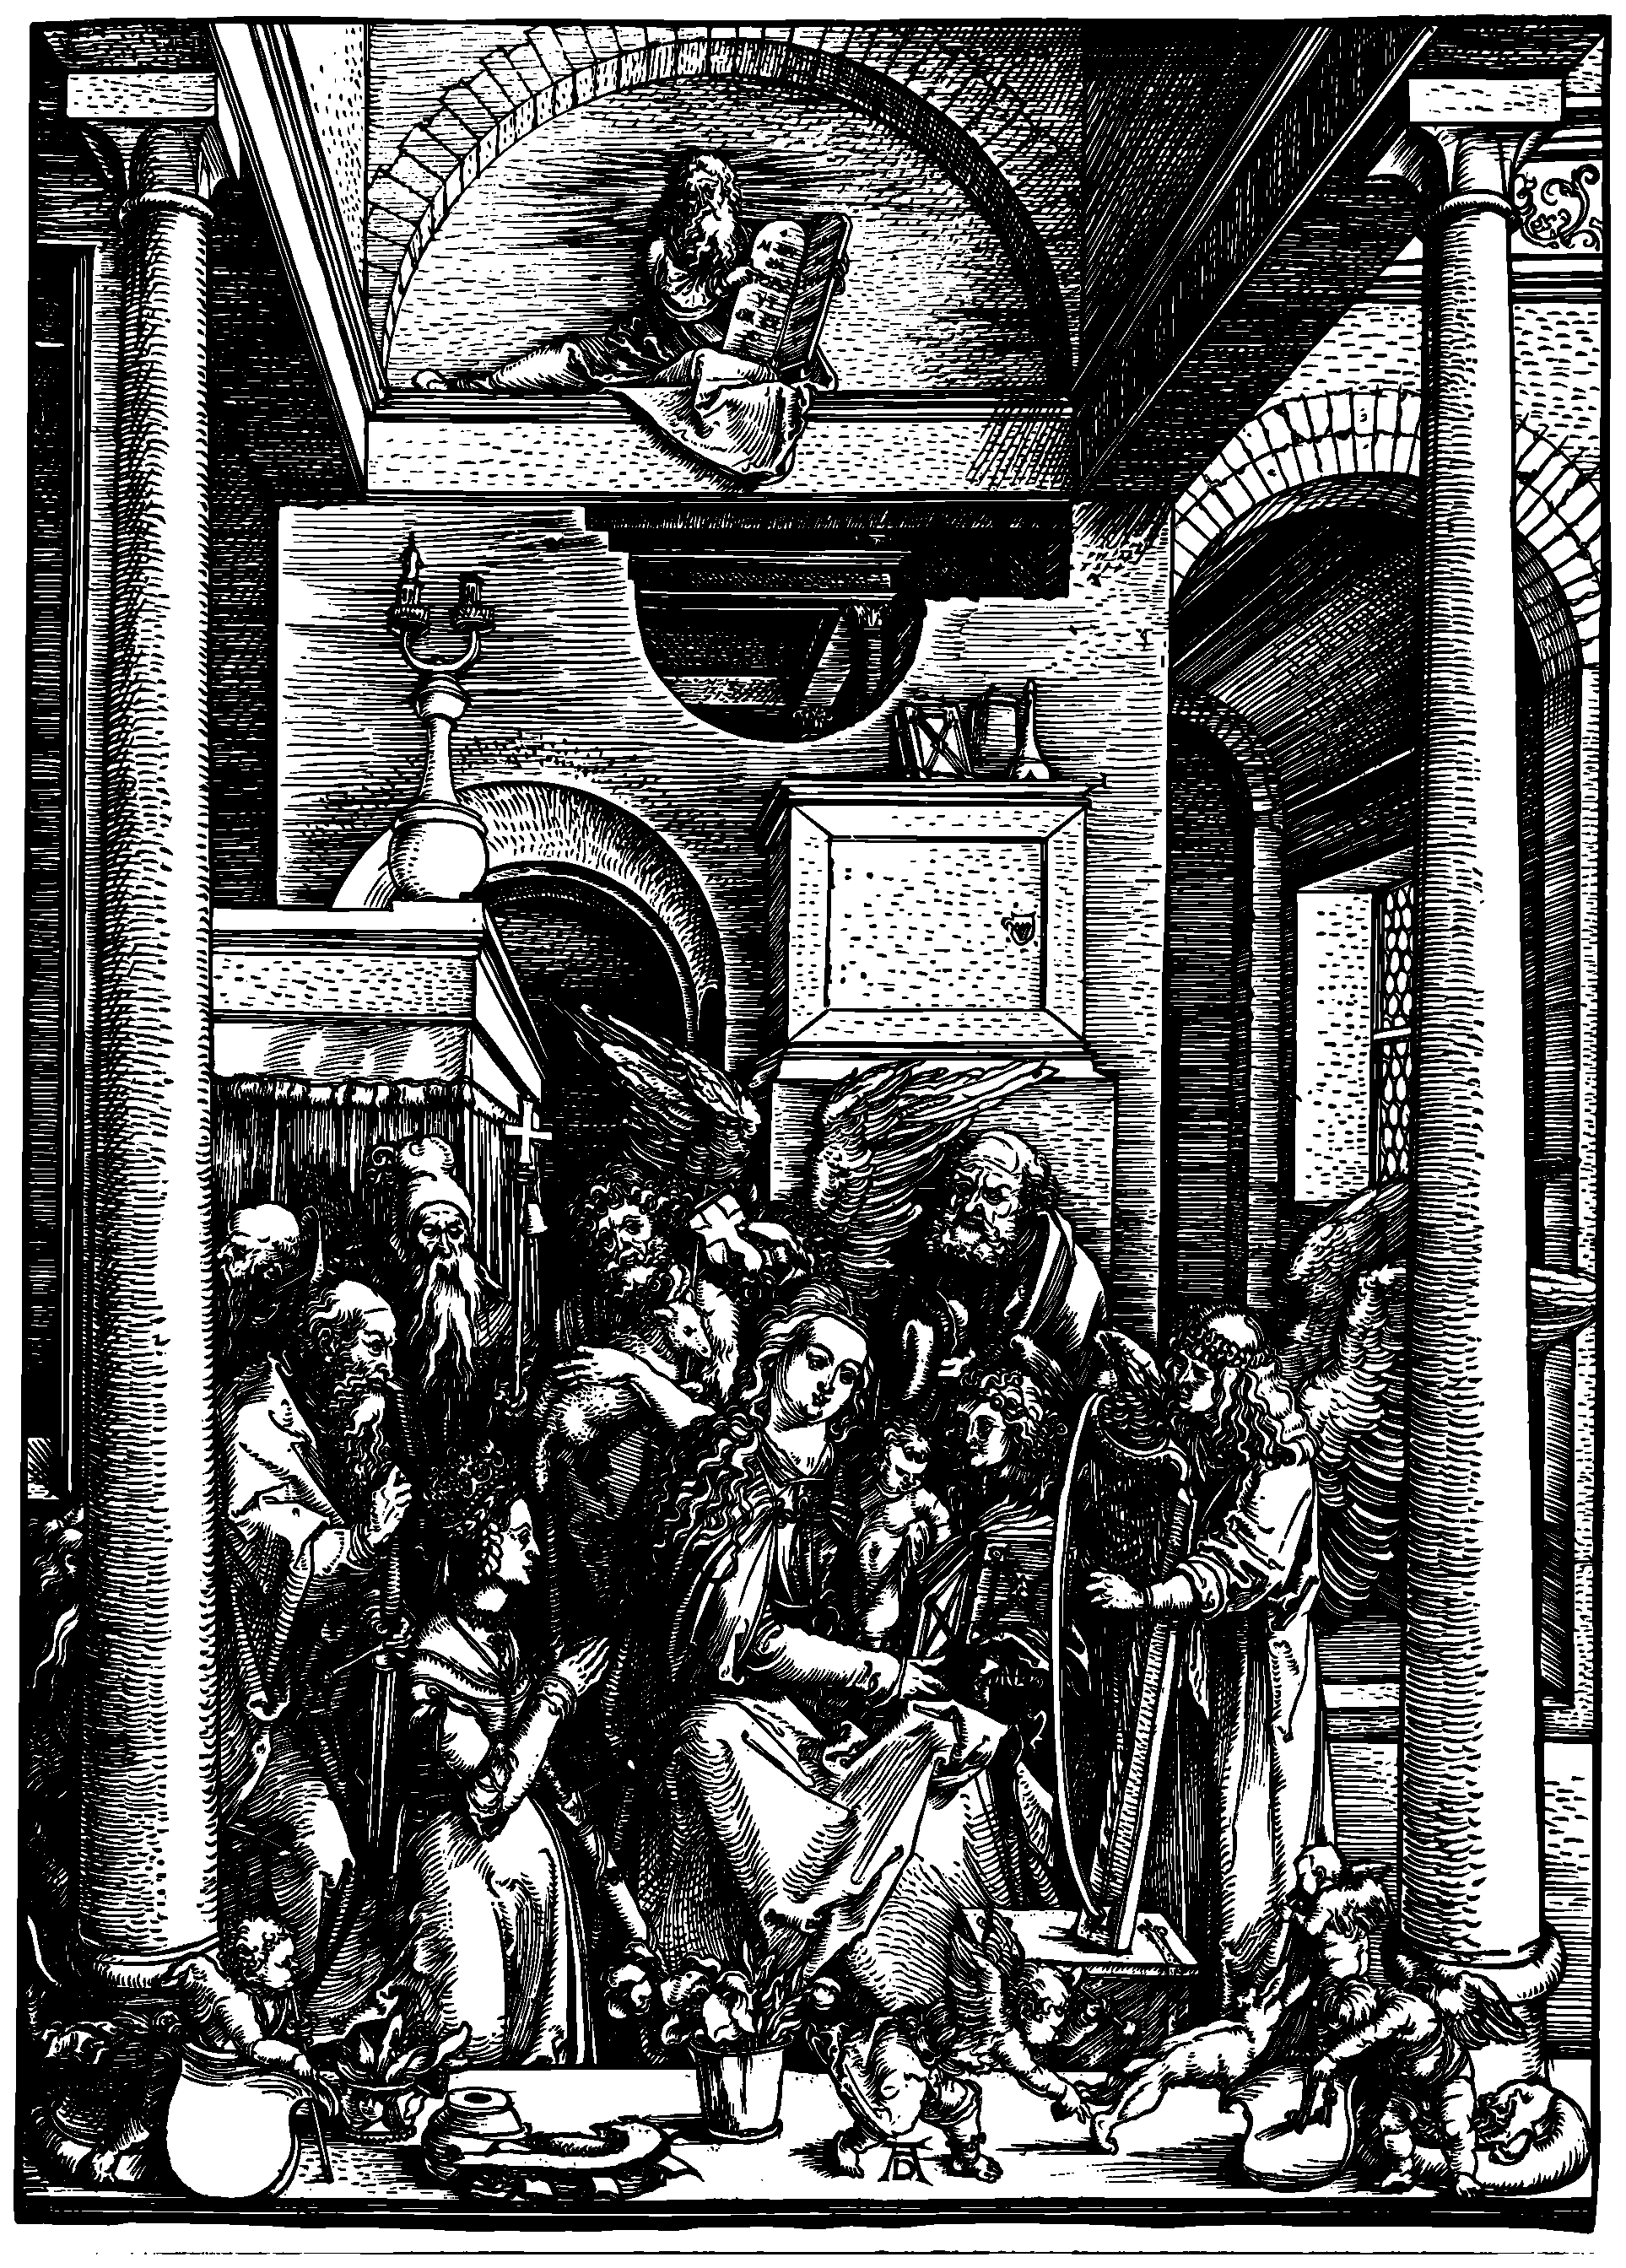
\includegraphics[width=98mm, height=140mm]{Commons/Saints.eps}
    \caption{\textsc{\Huge{Commons of the Saints}}}
\end{figure}
%\phantomsection
%\addcontentsline{toc}{section}{Common of Saints}
\fancyhead[RO,LE]{}
\fancyhead[RE,LO]{}
\fancyhead[C]{\LARGE Common of Saints}

\section{Commons of the Apostles}

\subsection{Common of Vigils of the Apostles}\label{CommonVigilApostles}
\fancyhead[RO,LE]{\textit{Apostolic Vigils}}

\collect
\lett{G}{rant,} we beseech thee, Almighty God: that the venerable solemnity of blessed \textit{N.} thine Apostle, which we here prevent, may increase our devotion and set forward our salvation. Through.
\begin{rubric}
	If, however, the preceding Collect has already been said, or for the commemoration of a Confessor Bishop, then the following is to be said.
\end{rubric}
\lett{W}{e} beseech thee, Almighty God: that as we do prevent the festival of blessed \textit{N.} thine Apostle, so he may implore thy mercy for us; that we being delivered from our iniquities, may likewise be defended against all adversities. Through.


\subsection{Common of the Apostles outside Eastertide}\label{CommonApostles}
\fancyhead[RO,LE]{\textit{Apostles}}

\begin{paracol}{2}[]
\sloppy

\firstEvensong

\psalmAntiphon{This is my commandment,~{\dag} that ye love one another, as I have loved you.}

%MANUAL ADJUSTMENT:
\vspace{-1\baselineskip}

\firstEvensongHymn\label{ApostlesEvensong}

\hymnLett{L}{et}\textls[-25]{ heav'n's exultant praises ring,}

\hymnSecondLine{And earth with joy responsive sing:}

\begin{hangparas}{1.25em}{1}

Th'Apostles' deeds and high estate

This festal-tide we celebrate.\\

2. O ye who, thron'd in glory dread,

Shall judge the living and the dead,

True lights, the world illumining,

Regard the suppliant prayer we bring.\\

3. The gates of heav'n, at your command,

To all or clos'd or open stand:

May we, at your august decree,

Be loos'd from our iniquity.\\

4. The pow'r, of old to you convey'd,

Sickness and health alike obey'd:

May ye our ailing souls once more

To strength and holiness restore;\\

5. That Christ, th'unerring Judge of doom,

When he at time's last end shall come,

May grant us, for his mercy's sake,

Of joys eternal to partake.\\

6. All laud to God the Father be;

All praise, eternal Son, to thee;

All glory, as is ever meet,

To God the Holy Paraclete. Amen.\\
\end{hangparas}

℣. Their sound is gone out into all lands.

℟. And their words into the ends of the world.

\antiphon{Mag.}{They will deliver you up~{\dag} to the councils, and they will scourge you in their synagogues; and ye shall be brought before governors and kings for my sake, for a testimony against them and the Gentiles.}

\switchcolumn

\mattins

\psalmAntiphon{Greater love hath no man~{\dag} than this, that a man lay down his life for his friends.}

%MANUAL ADJUSTMENT:
\vspace{-1\baselineskip}

\mattinsInvitatoryHymn\label{ApostlesInvitatory}

\hymnLett{T}{h\smash{'}eternal} gifts of Christ the King,

\hymnSecondLine{Th'Apostles' glory let us sing;}

\begin{hangparas}{1.25em}{1}

And all with hearts of gladness raise

Due hymns of thankful love and praise.\\

2. For they the Church's princes are,

Triumphant leaders in the war,

In heav'nly courts a warrior band,

True lights to lighten every land.\\

3. Theirs is the steadfast faith of saints,

And hope that never yields nor faints,

The love of Christ in perfect glow

That lays the prince of this world low.\\

4. In them the Father's glory shone,

In them the will of God the Son,

In them exults the Holy Ghost,

Through them rejoice the heav'nly host.\\

5. To thee, Redeemer, now we cry,

That thou wouldst join with them on high

Thy servants, who this grace implore,

For ever and for evermore. Amen.
\end{hangparas}


\begin{hymnRubric}
	Office Hymn of I Evensong.\label{ApostlesMattins}
\end{hymnRubric}

℣. They declared the work of God.

℟. And wisely considered of his doing.

\antiphon{Ben.}{Ye which have forsaken all,~{\dag} and followed me, shall receive an hundredfold, and shall inherit everlasting life.}

\fussy
\end{paracol}

\secondEvensong

\psalmAntiphon{Firmly stablished~{\dag} is their princedom: and highly honoured are thy friends, O God.}\\

\begin{rubric}
	Office Hymn \& Versicle of I Evensong.
\end{rubric}

\antiphon{Mag.}{Be ye valiant in warfare,~{\dag} and contend ye with the old serpent: and ye shall receive an eternal kingdom, alleluia.}


%MANUAL ADJUSTMENT:
\clearpage
\subsection{Common of the Apostles in Eastertide}\label{CommonApostlesEaster}
\fancyhead[RO,LE]{\textit{Apostles in Eastertide}}

\begin{paracol}{2}[]
\sloppy

\firstEvensong

\psalmAntiphon{Thy Saints,~{\dag} O Lord shall blossom as the lily, alleluia: and as the odour of balsam shall they be before thee, alleluia.}

\firstEvensongHymn\label{ApostlesEvensongEaster}

\hymnLett{T}{he} Apostles' hearts were full of pain

\hymnSecondLine{For their dear Lord so lately slain:}

\begin{hangparas}{1.25em}{1}

That Lord his servants' wicked train

With bitter scorn had dar'd arraign.\\

2. With gentle voice the Angel gave

The women tidings at the grave;

`Forthwith your Master shall ye see:

He goes before to Galilee.'\\

3. And while with fear and joy they press'd

To tell these tidings to the rest,

Their Lord, their living Lord, they meet,

And see his form, and kiss his feet.\\

4. Th' Eleven, when they hear, with speed

To Galilee forthwith proceed:

That there they may behold once more

The Lord's dear face, as oft before.\\

5. We pray thee, King with glory deck'd,

In this our Paschal joy, protect

From all that death would fain effect

Thy ransom'd flock, thine own elect.
\end{hangparas}

%MANUAL ADJUSTMENT:
\newpage

    \par\noindent
	\centerline{\rule{0.25\textwidth}{0.4pt}}
	\par\noindent
\begin{rubric}
	From Low Sunday, exclusive, until Ascension Thursday, exclusive:
\end{rubric}

\begin{hangparas}{1.25em}{1}
6. To thee who, dead, again dost live,

All glory, Lord, thy people give;

All glory, as is ever meet,

To Father and to Paraclete. Amen.
\end{hangparas}

\begin{rubric}
	From Ascension Thursday, inclusive, until Whitsunday, inclusive:
\end{rubric}

\begin{hangparas}{1.25em}{1}
6. All glory, Lord, to thee we pay,

Ascending o'er the stars to-day;

All glory, as is ever meet,

To Father and to Paraclete. Amen.
\end{hangparas}
    \par\noindent
	\centerline{\rule{0.25\textwidth}{0.4pt}}
	\par
℣. O ye holy and righteous, rejoice in the Lord, alleluia.

℟. God hath chosen you to him to be his inheritance, alleluia.

\antiphon{Mag.}{Light perpetual~{\dag} shall shine upon thy Saints, O Lord; and an ageless eternity, alleluia.}

\switchcolumn

\mattins

\psalmAntiphon{In the heavenly kingdom~{\dag} the Blessed have their dwelling-place, alleluia: and their rest for ever and ever, alleluia.}

%\mattinsInvitatoryHymn

\begin{hymnRubric}
	Invitatory Hymn of I Evensong.
\end{hymnRubric}

\mattinsOfficeHymn\label{ApostlesMattinsEaster}

\hymnLett{I}{n} this our bright and Paschal day

\hymnSecondLine{The sun shines out with purer ray,}

\begin{hangparas}{1.25em}{1}
When Christ, to earthly sight made plain,

The glad Apostles see again.\\

2. The wounds, the riven wounds he shows

In that his flesh with light that glows,

In loud accord both far and nigh

The Lord's arising testify.\\

3. O Christ, the King who lov'st to bless,

Do thou our hearts and souls possess;

To thee our praise that we may pay,

To whom our laud is due for aye.\\

4. We pray thee, King with glory decked,

In this our Paschal joy, protect

From all that death would fain effect

Thy ransomed flock, thine own elect.
\end{hangparas}

    \par\noindent
	\centerline{\rule{0.25\textwidth}{0.4pt}}
	\par\noindent
\begin{rubric}
	From Low Sunday, exclusive, until Ascension Thursday, exclusive:
\end{rubric}
\begin{hangparas}{1.25em}{1}
5. To thee who, dead, again dost live,

All glory, Lord, thy people give;

All glory, as is ever meet,

To Father and to Paraclete. Amen.
\end{hangparas}
\begin{rubric}
	From Ascension Thursday, inclusive, until Whitsunday, inclusive:
\end{rubric}
\begin{hangparas}{1.25em}{1}
5. All glory, Lord, to thee we pay,

Ascending o'er the stars to-day;

All glory, as is ever meet,

To Father and to Paraclete. Amen.
\end{hangparas}
    \par\noindent
	\centerline{\rule{0.25\textwidth}{0.4pt}}
	\par
℣. Right dear in the sight of the Lord, alleluia.

℟. Is the death of his Saints, alleluia.

\antiphon{Ben.}{Daughters of Jerusalem,~{\dag} come forth and behold the Martyrs with the diadems wherewith the Lord hath crowned them in the day of solemnity and rejoicing, alleluia, alleluia.}

\fussy
\end{paracol}

\secondEvensong

\psalmAntiphon{Then shall the righteous~{\dag} shine forth as the sun in the presence sun in the presence of God, alleluia.}

\begin{rubric}
	Office Hymn of I Evensong.
\end{rubric}

℣. Right dear in the sight of the Lord, alleluia.

℟. Is the death of his Saints, alleluia.

\antiphon{Mag.}{O ye holy and righteous,~{\dag} rejoice in the Lord, alleluia: God hath chosen you to him to be his inheritance, alleluia.}


%MANUAL ADJUSTMENT:
\clearpage
\section{Commons of Martyrs}

\section{Common of a Martyr outside Eastertide}\label{CommonMartyr}
\fancyhead[RO,LE]{\textit{Martyr}}

\begin{paracol}{2}[]
\sloppy

\firstEvensong

\psalmAntiphon{Whosoever shall confess me~{\dag} before men, him will I confess also before my Father.}

\firstEvensongHymn\label{MartyrEvensong}

\hymnLett{O}{f}\textls[-10]{ all thy warrior Saints, O Lord,}

\hymnSecondLine{\textls[-10]{The portion, crown, and great reward:}}

\begin{hangparas}{1.25em}{1}

From all transgressions set us free

Who sing thy Martyr's victory.\\

2. The pleasures of the world he spurned,

From sin's pernicious lures he turned;

Accounting them as transient all,

He reached at length thy heav'nly hall.\\

3. For thee through man' a woe he ran,

In man' a fight he played the man;

For thee his blood he dared to pour,

And thence hath joy for evermore.\\

4. We therefore pray thee, full of love,

Regard us from thy throne above:

On this thy Martyr's triumph day,

Wash every stain of sin away.\\

5. Enduring laud and praise be done

To God the Father, and the Son,

And to the Holy Paraclete,

For endless ages, as is meet. Amen.\\
\end{hangparas}

℣. Thou hast crowned him with glory and honour, O Lord. 

℟. And madest him to have dominion of the works of thy hands.

\antiphon{Mag.}{This is a Martyr~{\dag} who strove for his Master's precepts, even unto death: and feared not the words of evil men, forasmuch as he was stablished on a sure foundation.}

\switchcolumn

\mattins

\psalmAntiphon{He that followeth me~{\dag} shall not walk in darkness, but shall have the light of life, saith the Lord.}

%\mattinsInvitatoryHymn

\begin{hymnRubric}
	Invitatory Hymn of I Evensong.
\end{hymnRubric}

\mattinsOfficeHymn\label{MartyrMattins}

\hymnLett{T}{hou} foll'west, Martyr of thy God,

\hymnSecondLine{The path the only Son hath trod,}

\begin{hangparas}{1.25em}{1}
	
Thy conquered foes thou treadest down,

And gloriest in a victor's crown.\\

2. O may thy prayer for us obtain

The cleansing of each guilty stain,

Shield us from sin's contagious blight,

Put life's long weariness to flight.\\

3. The cruel chains are now unwound

That once thy sacred body bound, 

So may God's Son earth's fetters break

From us, for his own love's dear sake.\\

4. All laud to God the Father be;

All praise, eternal Son, to thee;

All glory, as is ever meet,

To God the Holy Paraclete. Amen.\\
\end{hangparas}

℣. The righteous shall flourish like a palm-tree.

℟. And shall spread abroad like a cedar in Libanus.

\antiphon{Ben.}{He that hateth his life~{\dag} in this world shall keep it unto life eternal.}

\fussy
\end{paracol}

\secondEvensong

\psalmAntiphon{If any man have served me,~{\dag} he shall be honoured of my Father which is in heaven, saith the Lord.}

\begin{rubric}
	Office Hymn of I Evensong.
\end{rubric}

℣. The righteous shall flourish like a palm-tree.

℟. And shall spread abroad like a cedar in Libanus.

\antiphon{Mag.}{Whosoever will come after me,~{\dag} let him deny himself, and take up his cross, and follow me.}

\collect\label{CommonMartyrBishopCollect}
\begin{inhead}
	Martyr Bishop
\end{inhead}
\lett{A}{lmighty} God, mercifully look upon our infirmities: that whereas we are oppressed by the burden of our sins, the glorious intercession of blessed \textit{N.} thy Martyr and Bishop may be our succour and defence. Through.
\begin{inhead}
	or,
\end{inhead}
\lett{O}{God,} who makest us glad with the yearly solemnity of blessed \textit{N.} thy Martyr and Bishop: mercifully grant; that, as we now celebrate his birthday, so we may likewise rejoice in his protection. Through.

\begin{inhead}\label{CommonMartyrNotBishopCollect}
	Martyr not Bishop
\end{inhead}
\lett{G}{rant,} we beseech thee, Almighty God: that we, who devoutly celebrate the birthday of blessed \textit{N.}, thy Martyr, may by his intercession be stablished in the love of thy name. Through.
\begin{inhead}
	or,
\end{inhead}
\lett{G}{rant,} we beseech thee, Almighty God: that, at the intercession of blessed \textit{N.}, thy Martyr, we may both be delivered from all adversities which may happen to the body, and from all evil thoughts, which may assault and hurt the soul. Through.


%MANUAL ADJUSTMENT:
\clearpage
\subsection{Common of Many Martyrs out of Eastertide}\label{CommonMartyrs}
\fancyhead[RO,LE]{\textit{Martyrs}}

\begin{paracol}{2}[]
\sloppy

\firstEvensong

\psalmAntiphon{The Blessed~{\dag} with their palms have entered into the kingdom; they have earned their diadems of glory from the hand of God.}

\firstEvensongHymn\label{MartyrsEvensong}

\hymnLett{T}{he} merits of the Saints,

\hymnSecondLine{Blessed for evermore.}

\hymnThirdLine{Their love that never faints,}

\begin{hangparas}{1.25em}{1}
The toils they bravely bore

For these the Church to-day

Pours forth her joyous lay:

These victors win the noblest bay.\\

2. They, whom this world of ill,

While it yet held, abhorred;

Its with'ring flow'rs that still 

They spurned with one accord:

They knew them short-lived all,

And followed at thy call,

King Jesu, to thy heav'nly hall.\\

3. For thee all pangs they bare,

Fury and mortal hate;

The cruel scourge to tear,

The hook to lacerate;

But vain their foes' intent:

For, every torment spent,

Their valiant spirits stood unbent.\\

4. Like sheep their blood they poured;

And without groan or tear,

They bent before the sword

For that their King most dear:

Their souls, serenely blest,

In patience they possess'd,

And looked in hope towards their rest.\\

5. What tongue may here declare, 

Fancy or thought descry,

The joys thou dost prepare 

For these thy Saints on high!

Empurpled in the flood

Of their victorious blood.

They won the laurel from their God.\\

6. To thee, O Lord Most High,

One in Three Persons still,

To pardon us we cry.

And to preserve from ill:

Here give thy servants peace,

Hereafter glad release. 

And pleasures that shall never cease. Amen.\\
\end{hangparas}

℣. Be glad, O ye righteous, and rejoice in the Lord.

℟. And be joyful, all ye that are true of heart.

\antiphon{Mag.}{For theirs is the kingdom of heaven,~{\dag} who despised worldly living: who have won the rewards of the kingdom, and have washed their robes in the blood of the Lamb.}

\switchcolumn

\mattins

\psalmAntiphon{These are the holy ones~{\dag} who, for the covenant of God, have delivered up their bodies, and have washed their robes in the blood of the Lamb.}

\mattinsInvitatoryHymn\label{MartyrsInvitatory}

\hymnLett{T}{he} Martyrs' triumphs let us sing,

\hymnSecondLine{Their blood pour'd forth for Christ the King,}

\begin{hangparas}{1.25em}{1}
And while due hymns of praise we pay,

Our thankful hearts cast grief away.\\

2. The world its terrors urg'd in vain;

They reck'd not of the body's pain;

One step, and holy death made sure

The life that ever shall endure.\\

3. To flames the Martyr Saints are hail'd;

By teeth of savage beasts assail'd;

Against them, armed with ruthless brand

And hooks of steel, their torturers stand.\\

4. The mangl'd frame is tortur'd sore,

The holy life-drops freshly pour;

They stand unmov'd amidst the strife,

By grace of everlasting life.\\

5. Redeemer, hear us of thy love,

That, with the Martyr host above,

Hereafter, of thine endless grace,

Thy servants also may have place. Amen.
\end{hangparas}

\mattinsOfficeHymn\label{MartyrsMattins}

\hymnLett{A}{ll} glorious King of Martyrs thou,

\hymnSecondLine{Crown of Confessors here below;}

\begin{hangparas}{1.25em}{1}
Whom, casting earthly joys away,

Thou guidest to celestial day.\\

2. Thine ear in mercy, Saviour, lend,

While unto thee our prayers ascend:

And as we count their triumphs won,

Forgive the sins that we have done.\\

3. Martyrs in thee their triumph gain;

From thee, Confessors grace obtain:

O'ercome in us the lust of sin,

That we thy pard'ning love may win.\\

4. All laud to God the Father be;

All praise, eternal Son, to thee;

All glory, as is ever meet,

To God the Holy Paraclete. Amen.\\
\end{hangparas}

℣. Let the Saints be joyful with glory.

℟. Let them rejoice in their beds.

\antiphon{Ben.}{The very hairs of your head~{\dag} are all numbered: fear ye not therefore, ye are of more value than many sparrows.}

\fussy
\end{paracol}


\secondEvensong

\psalmAntiphon{God shall wipe away all tears~{\dag} from the eyes of the Saints: and there shall be no more sorrow, neither crying, neither shall there be any more pain; for the former things are passed away.}

\begin{rubric}
	Office Hymn of I Evensong. Versicle of Mattins.
\end{rubric}

\antiphon{Mag.}{In the heavenly kingdom~{\dag} rejoice the souls of the Blessed, who followed the footsteps of Christ their Master: and since for love of him they poured forth their life-blood, therefore with Christ do they exult for ever.}

\collect\label{CommonMartyrsBishopsCollect}
\begin{inhead}
	Many Martyr Bishops
\end{inhead}
\lett{P}{rotect} us, O Lord, we beseech thee, who observe the feast of thy blessed Martyrs and Bishops \textit{N. and N.}: and grant that by their meritorious supplication we may find favour in thy sight. Through.

\begin{inhead}\label{CommonMartyrsNotBishopsCollect}
	Many Martyrs not Bishops
\end{inhead}
\lett{O}{God,} who vouchsafest unto us to celebrate the birthday of thy holy Martyrs
\textit{N. and N.}: grant that we may rejoice in the everlasting felicity of their fellowship. Through.
\begin{inhead}
	or,
\end{inhead}
\lett{O}{God,} who makest us glad with the yearly solemnity of thy holy Martyrs \textit{N. and N.}: mercifully grant; that as we do rejoice in their merits, so we may be enkindled by their example. Through.


\subsection{Common of a Martyr in Eastertide}\label{CommonMartyrEaster}
\fancyhead[RO,LE]{\textit{Martyr in Easter}}

\begin{paracol}{2}[]
\sloppy

\firstEvensong\label{MartyrEvensongEaster}

\psalmAntiphon{Thy blessed Saints, O Lord,~{\dag} cried out within the veil, alleluia, alleluia, alleluia.}

\firstEvensongHymn

\hymnLett{O}{f}\textls[-15]{ all thy warrior Saints, O Lord,}

\hymnSecondLine{The portion, crown, and great reward;}

\begin{hangparas}{1.25em}{1}
From all transgressions set us free

Who sing thy Martyr's victory.\\

2. The pleasures of the world he spurn'd,

From sin's pernicious lures he turn'd;

Accounting them as transient all,

He reached at length thy heav’nly hall.\\

3. For thee through man' a woe he ran,

In man' a fight he played the man;

For thee his blood he dar'd to pour,

And thence hath joy for evermore.\\

3. We therefore pray thee, full of love,

Regard us from thy throne above:

On this thy Martyr's triumph day,

Wash every stain of sin away.
\end{hangparas}

    \par\noindent
	\centerline{\rule{0.25\textwidth}{0.4pt}}
	\par\noindent
\begin{rubric}
	From Low Sunday, exclusive, until Ascension Thursday, exclusive:
\end{rubric}

\begin{hangparas}{1.25em}{1}
4. To thee who, dead, again dost live,

All glory, Lord, thy people give;

All glory, as is ever meet,

To Father and to Paraclete. Amen.
\end{hangparas}

\begin{rubric}
	From Ascension Thursday, inclusive, until Whitsunday, inclusive:
\end{rubric}

\begin{hangparas}{1.25em}{1}
4. All glory, Lord, to thee we pay,

Ascending o'er the stars to-day;

All glory, as is ever meet,

To Father and to Paraclete. Amen.
\end{hangparas}

    \par\noindent
	\centerline{\rule{0.25\textwidth}{0.4pt}}
	\par
℣. O ye holy and righteous, rejoice in the Lord, alleluia.

℟. God hath chosen you to him to be his inheritance, alleluia.

\antiphon{Mag.}{Light perpetual~{\dag} shall shine upon thy Saints, O Lord; and an ageless eternity, alleluia.}

\switchcolumn

\mattins

\psalmAntiphon{O ye spirits and souls~{\dag} of the righteous, sing a hymn unto the Lord our God, alleluia, alleluia.}

%\mattinsInvitatoryHymn
\begin{hymnRubric}
	Invitatory Hymn of I Evensong.
\end{hymnRubric}

\mattinsOfficeHymn\label{MartyrMattinsEaster}

\hymnLett{T}{hou} foll'west, Martyr of thy God,

\hymnSecondLine{The path the only Son hath trod,}

\begin{hangparas}{1.25em}{1}
Thy conquer'd foes thou treadest down,

And gloriest in a victor's crown.\\

2. O may thy prayer for us obtain

The cleansing of each guilty stain,

Shield us from sin's contagious blight,

Put life's long weariness to flight.\\

3. The cruel chains are now unwound

That once thy sacred body bound,

So may God's Son earth's fetters break

From us, for his own love's dear sake.
\end{hangparas}

    \par\noindent
	\centerline{\rule{0.25\textwidth}{0.4pt}}
	\par\noindent
\begin{rubric}
	From Low Sunday, exclusive, until Ascension Thursday, exclusive:
\end{rubric}

\begin{hangparas}{1.25em}{1}
4. To thee who, dead, again dost live,

All glory, Lord, thy people give;

All glory, as is ever meet,

To Father and to Paraclete. Amen.
\end{hangparas}

\begin{rubric}
	From Ascension Thursday, inclusive, until Whitsunday, inclusive:
\end{rubric}

\begin{hangparas}{1.25em}{1}
4. All glory, Lord, to thee we pay,

Ascending o'er the stars to-day;

All glory, as is ever meet,

To Father and to Paraclete. Amen.
\end{hangparas}

    \par\noindent
	\centerline{\rule{0.25\textwidth}{0.4pt}}
	\par
	
	℣. Right dear in the sight of the Lord, alleluia.

	℟. Is the death of his Saints, alleluia.

\antiphon{Ben.}{Daughters of Jerusalem,~{\dag} come forth and behold the Martyrs with the diadems wherewith the Lord hath crowned them in the day of solemnity and rejoicing, alleluia, alleluia.}

\fussy
\end{paracol}

\secondEvensong

\psalmAntiphon{Then shall the righteous~{\dag} shine forth as the sun in the presence sun in the presence of God, alleluia.}

\begin{rubric}
	Office Hymn of I Evensong.
\end{rubric}

℣. Right dear in the sight of the Lord, alleluia.

℟. Is the death of his Saints, alleluia.

\antiphon{Mag.}{O ye holy and righteous,~{\dag} rejoice in the Lord, alleluia: God hath chosen you to him to be his inheritance, alleluia.}

\collect

\begin{inhead}\label{CommonMartyrBishopEasterCollect}
	Martyr Bishop
\end{inhead}
\lett{A}{lmighty} God, mercifully look upon our infirmities: that whereas we are oppressed by the burden of our sins, the glorious intercession of blessed \textit{N.} thy Martyr and Bishop may be our succour and defence. Through.

\begin{inhead}
	or,
\end{inhead}
\lett{O}{God,} who makest us glad with the yearly solemnity of blessed \textit{N.}, thy Martyr and Bishop: mercifully grant; that as we now devoutly celebrate his birthday, so we may likewise rejoice in his protection. Through.

\begin{inhead}\label{CommonMartyrNotBishopEasterCollect}
	Martyr not Bishop
\end{inhead}
\lett{G}{rant,} we beseech thee, Almighty God: that we, who devoutly celebrate the birthday of blessed \textit{N.}, thy Martyr; may by his intercession be stablished in the love of thy name. Through.
\begin{inhead}
	or,
\end{inhead}
\lett{G}{rant,} we beseech thee, Almighty God: that at the intercession of blessed \textit{N.} thy Martyr, we may both be delivered from all adversities which may happen to the body, and from all evil thoughts which may assault and hurt the soul. Through.



%MANUAL ADJUSTMENT:
\clearpage
\subsection{Common of Many Martyrs in Eastertide}\label{CommonMartyrsEaster}
\fancyhead[RO,LE]{\textit{Martyrs in Easter}}

\begin{paracol}{2}[]
\sloppy


\firstEvensong


\psalmAntiphon{Thy blessed Saints, O Lord,~{\dag} cried out within the veil, alleluia, alleluia, alleluia.}

\firstEvensongHymn\label{MartyrsEvensongEaster}

\hymnLett{A}{ll} glorious King of Martyrs thou,

\hymnSecondLine{Crown of Confessors here below,}

\begin{hangparas}{1.25em}{1}
Whom, casting earthly joys away,

Thou guidest to celestial day:\\

2. Thine ear in mercy, Saviour, lend,

While unto thee our prayers ascend:

And as we count their triumphs won,

Forgive the sins that we have done.\\

3. Martyrs in thee their triumph gain;

From thee, Confessors grace obtain:

O'ercome in us the lust of sin,

That we thy pard'ning love may win.
\end{hangparas}

    \par\noindent
	\centerline{\rule{0.25\textwidth}{0.4pt}}
	\par\noindent
\begin{rubric}
	From Low Sunday, exclusive, until Ascension Thursday, exclusive:
\end{rubric}

\begin{hangparas}{1.25em}{1}
4. To thee who, dead, again dost live,

All glory, Lord, thy people give;

All glory, as is ever meet,

To Father and to Paraclete. Amen.
\end{hangparas}

\begin{rubric}
	From Ascension Thursday, inclusive, until Whitsunday, inclusive:
\end{rubric}

\begin{hangparas}{1.25em}{1}
4. All glory, Lord, to thee we pay,

Ascending o'er the stars to-day;

All glory, as is ever meet,

To Father and to Paraclete. Amen.
\end{hangparas}

    \par\noindent
	\centerline{\rule{0.25\textwidth}{0.4pt}}
	\par
	
	℣. O ye holy and righteous, rejoice in the Lord, alleluia.

	℟. God hath chosen you to him to be his inheritance, alleluia.

\antiphon{Mag.}{Light perpetual~{\dag} shall shine upon thy Saints, O Lord; and an ageless eternity, alleluia.}

\switchcolumn

\mattins

\psalmAntiphon{O ye spirits and souls~{\dag} of the righteous, sing a hymn unto the Lord our God, alleluia, alleluia.}

%\mattinsInvitatoryHymn

\begin{hymnRubric}
	Invitatory Hymn \blackrubric{of the Common of Many Martyrs} (p. \pageref{MartyrsInvitatory}).
\end{hymnRubric}

\begin{hymnRubric}
	Office Hymn of I Evensong.
\end{hymnRubric}

	℣. Right dear in the sight of the Lord, alleluia.

	℟. Is the death of his Saints, alleluia.

\antiphon{Ben.}{Daughters of Jerusalem,~{\dag} come forth and behold the Martyrs with the diadems wherewith the Lord hath crowned them in the day of solemnity and rejoicing, alleluia, alleluia.}

\secondEvensong

\psalmAntiphon{Then shall the righteous~{\dag} shine forth as the sun in the presence sun in the presence of God, alleluia.}

\begin{rubric}
	Office Hymn of I Evensong.
\end{rubric}

℣. Right dear in the sight of the Lord, alleluia.

℟. Is the death of his Saints, alleluia.

\antiphon{Mag.}{O ye holy and righteous,~{\dag} rejoice in the Lord, alleluia: God hath chosen you to him to be his inheritance, alleluia.}

\fussy
\end{paracol}

\collect\label{CommonMartyrsBishopsEasterCollect}
\begin{inhead}
	Martyrs Bishops
\end{inhead}
\lett{P}{rotect} us, O Lord, we beseech thee, who observe the feast of thy blessed Martyrs and Bishops \textit{N. and N.}: and grant that by their meritorious supplication we may ever find favour in thy sight. Through.

\begin{inhead}\label{CommonMartyrsNotBishopsEasterCollect}
	Many Martyrs not Bishops
\end{inhead}
\lett{O}{God,} who vouchsafest unto us to celebrate the birthday of thy holy Martyrs \textit{N. and N.}: grant that we may rejoice in the everlasting felicity of their fellowship. Through.
\begin{inhead}
	or,
\end{inhead}
\lett{O}{God,} who makest us glad with the yearly solemnity of thy holy Martyrs \textit{N. and N.}: mercifully grant that as we rejoice in their merits, so we may be enkindled by their example. Through.



%MANUAL ADJUSTMENT:
\clearpage%Page 439
\section{Commons for Confessors}

\subsection{Common of a Confessor Bishop}\label{CommonConfessorBishop}
\fancyhead[RO,LE]{\textit{Confessor Bishop}}

\begin{paracol}{2}[]
\sloppy

\firstEvensong\label{ConfessorBishopEvensong}

\psalmAntiphon{Behold a great priest,~{\dag} who in his days pleased God, and was found righteous.}

\firstEvensongHymn
\hymnLett{T}{his} the Confessor of the Lord, whose triumph

\hymnSecondLine{Now through the wide world celebrate the faithful,}

    \par\noindent
	\centerline{\rule{0.25\textwidth}{0.4pt}}
	\par\noindent
\begin{plainRubric}
	Unless it not be the day of the Saint’s death (that is, the Proper is marked with the letters \blackrubric{m.t.v.}), the following reads,
\end{plainRubric}

\begin{hangparas}{1.25em}{1}
Merited this day joyfully to enter

Heavenly mansions.
\end{hangparas}
    \par\noindent
	\centerline{\rule{0.25\textwidth}{0.4pt}}
	\par\noindent
	
\begin{plainRubric}
	If it be not the day of the Saint’s death (indicated in the Proper by the letters, \blackrubric{m.t.v.}), the following reads,
\end{plainRubric}

\begin{hangparas}{1.25em}{1}
On this his feast-day, year by year receiveth

Merited honours.
\end{hangparas}

    \par\noindent
	\centerline{\rule{0.25\textwidth}{0.4pt}}
	\par\noindent
\begin{hangparas}{1.25em}{1}
2. Saintly and prudent, continent and humble,

Chaste was he ever, peaceable and sober,

While living vigour, coursing through his body,

Quicken'd his being.\\

3. When to his honour'd sepulchre, with members

Languishing sorely, sufferers resorted,

Oft unto wholeness did the Lord restore them

At his petition.\\

4. Wherefore our chorus chanteth in his honour

Here, on his feast-day, this most willing anthem;

That in his merits we may have our portion

Now and for ever.\\

5. His be the glory, power, and salvation,

Who, o'er the heavens, dwelling in the highest,

Earth's mighty fabric ruleth and directeth,

Onely and Trinal. Amen.\\
\end{hangparas}

℣. The Lord loved him and adorned him.

℟. He clothed him with a robe of glory.

\begin{inhead}
	Doctor
\end{inhead}
\antiphon{Mag.}{O Teacher right excellent,~{\dag} O light of Holy Church, O blessed \textit{N.}, lover of the divine law: intercede for us unto the Son of God.}
\begin{inhead}
	Not a Doctor
\end{inhead}
\antiphon{Mag.}{O thou Priest and Bishop,~{\dag} thou worker of mighty works, thou good shepherd of the people, pray unto the Lord for us.}

\switchcolumn

\mattins

\psalmAntiphon{There was none~{\dag} like unto him, who kept the law of the Most High.}

\begin{rubric}
	Invitatory Hymn of I Evensong.
\end{rubric}

\mattinsOfficeHymn\label{ConfessorBishopMattins}

\hymnLett{J}{esu,}\textls[-30]{ the world's Redeemer, hear;}

\hymnSecondLine{Thy Bishop's fadeless Crown, draw near:}

\begin{hangparas}{1.25em}{1}
Accept with gentlest love to-day

The prayers and praises that we pay.\\

2. This meek Confessor of thy Name

To-day attain'd a glorious fame;

Whose yearly feast, in solemn state,

Thy faithful people celebrate.\\

3. The world and all its boasted good,

As vain and passing, he eschew'd;

And therefore with Angelic bands

In endless joy for ever stands.\\

4. Grant then that we, most gracious God,

May follow in the steps he trod:

And at his prayer thy servants free

From stain of all iniquity.\\

5. To thee, O Christ, our loving King,

All glory, praise, and thanks we bring:

All glory, as is ever meet,

To Father and to Paraclete. Amen.\\
\end{hangparas}

℣. The Lord guided the righteous in right paths.

℟. And shewed him the kingdom of God.

\antiphon{Ben.}{Well done,~{\dag} thou good and faithful servant: thou hast been faithful over a few things, I will make thee ruler over many things, saith the Lord.}

\secondEvensong

\psalmAntiphon{Good and faithful servant,~{\dag} enter thou into the joy of thy Lord.}

\begin{rubric}
	Office Hymn of I Evensong. Versicle of Mattins.
\end{rubric}

\begin{inhead}
	Doctor
\end{inhead}
\antiphon{Mag.}{O Teacher right excellent,~{\dag} O light of Holy Church, O blessed \textit{N.}, lover of the divine law: intercede for us unto the Son of God.}
\begin{inhead}
	Not a Doctor
\end{inhead}
\antiphon{Mag.}{I will liken him~{\dag} unto a wise man, which built his house upon a rock.}

\fussy
\end{paracol}

%MANUAL ADJUSTMENT:
\clearpage
\collect
\begin{inhead}\label{ConfessorBishopDoctorCollect}
	Confessor Bishop Doctor
\end{inhead}
\lett{O}{God,} who didst give blessed \textit{N.} unto thy people to be a minister of everlasting salvation: grant, we beseech thee; that as we have learned of him the doctrine of life on earth, so we may be found worthy to have him for our advocate in heaven. Through.

\begin{inhead}\label{ConfessorBishopCollect}
	Confessor Bishop Not a Doctor
\end{inhead}
\lett{G}{rant,} we beseech thee, Almighty God: that the venerable solemnity of blessed \textit{N.}, thy Confessor and Bishop may increase our devotion and set forward our salvation. Through.
\begin{inhead}
	or,
\end{inhead}
\lett{O}{God,} who didst give blessed \textit{N.} unto thy people to be a minister of everlasting salvation: grant, we beseech thee; that as we have learned of him the doctrine of life on earth, so we may be found worthy to have him for our advocate in heaven. Through.


\subsection{Common of a Confessor not a Bishop}\label{CommonConfessorNotBishop}
\fancyhead[RO,LE]{\textit{Confessor not Bishop}}

\begin{paracol}{2}[]
\sloppy

\firstEvensong

\psalmAntiphon{Lord, thou deliveredst~{\dag} unto me five talents: behold, I have gained beside them five talents more.}

%\firstEvensongHymn

\begin{rubric}
	Office Hymn \blackrubric{of the Common of a Confessor Bishop} (p. \pageref{ConfessorBishopEvensong}).
\end{rubric}
	
	℣. The Lord loved him and adorned him.

	℟. He clothed him with a robe of glory.
	
\begin{inhead}
	Confessor Doctor
\end{inhead}
\antiphon{Mag.}{O Teacher right excellent,~{\dag} O light of Holy Church, O blessed \textit{N.}, lover of the divine law: intercede for us unto the Son of God.}

\begin{inhead}
	Confessor not a Doctor
\end{inhead}
\antiphon{Mag.}{I will liken him~{\dag} unto a wise man, which built his house upon a rock.}

\secondEvensong

\psalmAntiphon{Blessed is that servant~{\dag} whom his Lord, when he cometh and knocketh at the door, shall find watching.}

\begin{rubric}
	Office Hymn of I Evensong \blackrubric{from the Common of a Confessor Bishop} (p. \pageref{ConfessorBishopEvensong}).
\end{rubric}

℣. The Lord guided the righteous in right paths.

℟. And shewed him the kingdom of God.

\begin{inhead}
	Confessor Doctor
\end{inhead}
\antiphon{Mag.}{O Teacher right excellent,~{\dag} O light of Holy Church, O blessed \textit{N.}, lover of the divine law: intercede for us unto the Son of God.}

\begin{inhead}
	Confessor not a Doctor
\end{inhead}
\antiphon{Mag.}{The world, and all things earthly,~{\dag} this man despised, triumphant: he laid up treasures in heaven by word and deed.}

\switchcolumn

\mattins

\psalmAntiphon{A wise and faithful servant,~{\dag} whom the Lord hath made ruler over all his household.}


\begin{rubric}
	Invitatory Hymn of I Evensong \blackrubric{from the Common of a Confessor Bishop} (p. \pageref{ConfessorBishopEvensong})
\end{rubric}

\mattinsOfficeHymn\label{ConfessorNotBishopMattins}

\hymnLett{O}{Jesu,} Crown above the sky,

\hymnSecondLine{Thou everlasting Truth most high,}

\begin{hangparas}{1.25em}{1}
Who dost to thy Confessor give

Rewards with those that ever live:\\

2. Thy lowly band of suppliants spare;

O may we, holpen by his prayer,

Remission of our sins obtain

And freedom from each binding chain.\\

3. Again the slowly circling year

The day of glory bringeth here

Whereon thy Saint, from flesh set free,

In pow'r ascended up to thee.\\

4. He deem'd the vain delights of earth,

Its boasted glories, little worth;

And spurning them as tainted, pass'd

To heav'n's triumphant joy at last.\\

5. By ever owning thee his King,

O Christ most gracious, did he fling

The haughty foe beneath his feet,

And all his minions bravely beat.\\

6. Renown'd for faith and virtue, he

Confess'd his Lord so constantly,

And with such fasts his flesh subdued

That he obtain'd supernal food.\\

7. O thou, most full of love and grace,

We humbly fall before thy face;

For this thy servant's sake, we pray,

Wipe all the debt we owe away.\\

8. Glory to thee, O Father, Lord,

And to thy Sole-begotten Word,

Both with the Holy Spirit One

While everlasting ages run. Amen.\\
\end{hangparas}

℣. The Lord guided the righteous in right paths.

℟. And shewed him the kingdom of God.

\antiphon{Ben.}{Well done, good and faithful servant,~{\dag} thou hast been faithful over a few things, I will make thee ruler over many things: enter thou into the joy of thy Lord.}

\fussy
\end{paracol}

\collect
\begin{inhead}\label{AbbotCollect}
	Abbot
\end{inhead}
\lett{W}{e} beseech thee, O Lord, that the prayers of the blessed Abbot, \textit{N.} may commend us unto thee: that by his advocacy thou wouldest vouchsafe unto us those things to which by our own merits we cannot obtain. Through.

\begin{inhead}\label{DoctorCollect}
	Doctor
\end{inhead}
\lett{O}{God,} who didst give blessed \textit{N.} unto thy people to be a minister of everlasting salvation: grant, we beseech thee; that as we have learned of him the doctrine of life on earth, so we may be found worthy to have him for our advocate in heaven. Through.

\begin{inhead}\label{ConfessorNotBishopCollect}
	Neither Abbot nor Doctor
\end{inhead}
\lett{O}{God,} who makest us glad with the yearly solemnity of blessed \textit{N.}, thy Confessor: mercifully grant; that, as we now celebrate his birthday, so we may follow the example of his life. Through.
\begin{inhead}
	or,
\end{inhead}
\lett{A}{ssist} us mercifully, O Lord, in these our supplications which we make before thee on the solemnity of blessed \textit{N.}, thy Confessor: that we, who put not our trust in our own righteousness, may be succoured by the prayers of him who found favour in thy sight. Through.


%\subsection{Common of Doctors}\label{CommonDoctors}
%\fancyhead[RO,LE]{\textit{Doctors}}
%
%\begin{rubric}
%	The Hymns \& Antiphons are from the closest relevant Common, except for the \blackrubric{Magnificat} Antiphon, as followeth.
%\end{rubric}
%
%\antiphon{Mag.}{O Teacher right excellent,~{\dag} O light of Holy Church, O blessed \textit{N.}, lover of the divine law: intercede for us unto the Son of God.}
%
%\collect
%\lett{O}{God,} who didst give blessed \textit{N.} unto thy people to be a minister of everlasting salvation: grant, we beseech thee; that as we have learned of him the doctrine of life on earth, so we may be found worthy to have him for our advocate in heaven. Through.



%\subsection{Common of Abbots}\label{CommonAbbots}
%\fancyhead[RO,LE]{\textit{Abbots}}
%
%
%\begin{rubric}
%	The Hymns \& Antiphons are as in the First Common of a Confessor not a Bishop (p. \pageref{CommonConfessorNotBishop}).
%\end{rubric}
%
%\collect
%\lett{W}{e} beseech thee, O Lord, that the prayers of the blessed Abbot, \textit{N.} may commend us unto thee: that by his advocacy thou wouldest vouchsafe unto us those things to which by our own merits we cannot obtain. Through.


%MANUAL ADJUSTMENT:
\clearpage
\section{Commons for Holy Women}

\subsection{Common of Virgins}\label{CommonVirgin}
\fancyhead[RO,LE]{\textit{Virgins}}

\begin{paracol}{2}[]
\sloppy

\firstEvensong

\psalmAntiphon{This is a wise Virgin,~{\dag} whom the Lord hath found watching.}

\firstEvensongHymn

\hymnLett{J}{esu,} the Virgins' Crown, do thou

\hymnSecondLine{Accept us, as in prayer we bow;}

\begin{hangparas}{1.25em}{1}
Born of that Virgin, whom alone

The Mother and the Maid we own.\\

2. Amongst the lilies thou dost feed,

With Virgin choirs accompanied;

With glory deck'd, the spotless brides

Whose bridal gifts thy love provides.\\

3. They, wheresoe'er thy footsteps bend.

With hymns and praises still attend;

In blessed troops they follow thee,

With dance, and song, and melody.\\

4. We pray thee therefore to bestow

Upon our senses here below

Thy grace, that so we may endure

From taint of all corruption pure.\\

5. To God the Father, God the Son,

And God the Spirit, Three in One,

Laud, honour, might, and glory be

From age to age eternally. Amen.\\
\end{hangparas}

%MANUAL ADJUSTMENT:
\newpage

℣. In thy grace and in thy beauty.

℟. Go forth, ride prosperously, and reign.

\begin{inhead}
	One Virgin
\end{inhead}
\antiphon{Mag.}{Come thou Bride of Christ,~{\dag} receive the crown which the Lord hath prepared for thee for ever.}

\begin{inhead}
	Many Virgins
\end{inhead}
\antiphon{Mag.}{O ye wise Virgins,~{\dag} arise and trim your lamps: for behold the Bridegroom cometh; go ye out to meet him.}


\secondEvensong

\psalmAntiphon{This woman~{\dag} is beautiful among the daughters of Jerusalem.}

\begin{rubric}
	Office Hymn of I Evensong. Versicle of Mattins.
\end{rubric}

\antiphon{Mag.}{Come thou Bride of Christ,~{\dag} receive the crown which the Lord hath prepared for thee for ever.}


\switchcolumn

\mattins

\psalmAntiphon{Blessed is the barren~{\dag} that is undefiled; she shall have fruit in the visitation of holy souls.}

\mattinsInvitatoryHymn\label{VirginInvitatory}

\hymnLett{S}{on} of a Virgin, Maker of thy Mother,

\hymnSecondLine{Thou, Rod and Blossom from a Stem unstained,}

\begin{hangparas}{1.25em}{1}
Now while a Virgin fair of fame we honour,

Hear our devotion!
\end{hangparas}

    \par\noindent
	\centerline{\rule{0.25\textwidth}{0.4pt}}
	\par\noindent
	\begin{rubric}
		The following stanzas are not said for a Virgin not a Martyress.
	\end{rubric}

\begin{hangparas}{1.25em}{1}	
2. Lo, on thy handmaid fell a twofold blessing,

Who, in her body vanquishing the weakness,

In that same body, grace from heav'n obtaining,

Bore the world witness.\\

3. Death, nor the rending pains of death appall'd her;

Bondage and torment found her undefeated:

So by the shedding of her blood attain'd she

Heavenly guerdon.
\end{hangparas}

	\par\noindent
	\centerline{\rule{0.25\textwidth}{0.4pt}}
	\par
	%MANUAL ADJUSTMENT:
\newpage
\begin{hangparas}{1.25em}{1}
4. Fountain of mercy, hear the prayers she offers;

Purge our offences, pardon our transgressions,

So that hereafter we to thee may render

Praise with thanksgiving.\\

5. Thou, the All-Father, thou the One-Begotten,

Thou, Holy Spirit, Three in One co-equal,

Glory be henceforth thine through all the ages,

World without ending. Amen.
\end{hangparas}

%\mattinsOfficeHymn

\begin{rubric}
	Office Hymn of I Evensong.\label{VirginMattins}
\end{rubric}

℣. Full of grace are thy lips.

℟. Because God hath blessed thee for ever.

\antiphon{Ben.}{The kingdom of heaven~{\dag} is likened unto a merchantman seeking goodly pearls; who, when he had found one pearl of great price, went and sold all that he had, and bought it.}\par

\end{paracol}

\collect\label{VirginMartyressCollect}
\begin{inhead}
	One Virgin Martyress
\end{inhead}
\lett{O}{God,} who among the manifold works of thy power hast bestowed even upon the weakness of women the victory of martyrdom: mercifully grant; that we, who celebrate the birthday of blessed \textit{N.} thy Virgin and Martyress, may by her example be drawn nearer unto thee. Through.
\begin{inhead}
	or,
\end{inhead}
\lett{W}{e} beseech thee, O Lord, that, like as blessed \textit{N.}, thy Virgin and Martyress, was ever found pleasing unto thee, both by the merit of her chastity, and by her confession of thy power: so she may implore for us thy pardon. Through.

%MANUAL ADJUSTMENT:
\clearpage
\begin{inhead}\label{VirginMartyressesCollect}
	Many Virgin Martyresses
\end{inhead}
\lett{G}{rant,} we beseech thee, O Lord our God, that we may at all times so devoutly honour the triumphs of thy holy Virgins and Martyresses \textit{N. and N.}: that, although we cannot worthily shew forth their praises, yet we may continually honour them with lowly service. Through.

\begin{inhead}\label{VirginOnlyCollect}
	One Virgin not a Martyress
\end{inhead}
\lett{G}{raciously} hear us, O God of our salvation: that, like as we do rejoice in the festival of blessed \textit{N.}, thy Virgin; so we may be instructed in all godly and devout affection. Through.
\begin{inhead}
	or,
\end{inhead}
\lett{G}{raciously} hear us, O God of our salvation: that, like as we do rejoice in the festival of blessed \textit{N.}, thy Virgin, so we may be instructed in all godly and devout affection. Through.


\subsection{Common of Holy Matrons}\label{CommonHolyMatrons}
\fancyhead[RO,LE]{\textit{Holy Matrons}}

\begin{paracol}{2}[]
\sloppy

\firstEvensong

\psalmAntiphon{While the King~{\dag} sitteth at his table, my spikenard sendeth forth a sweet-smelling savour.}

\begin{rubric}
	Office Hymn of Mattins.
\end{rubric}

\begin{inhead}
	One Martyress not a Virgin
\end{inhead}
℣. In thy grace and in thy beauty.

℟. Go forth, ride prosperously, and reign.

\antiphon{Mag.}{The kingdom of heaven~{\dag} is likened unto a merchantman seeking goodly pearls; who, when he had found one pearl of great price, went and sold all that he had, and bought it.}

\begin{inhead}
	Many Martyresses not Virgins
\end{inhead}
℣. Thou hast crowned them with glory and honour, O Lord.

℟. And madest them to have dominion of the works of thy hands.

\antiphon{Mag.}{For theirs is the kingdom of heaven,~{\dag} who despised worldly living: who have won the rewards of the kingdom, and have washed their robes in the blood of the Lamb.}

\secondEvensong

\psalmAntiphon{This woman~{\dag} is beautiful among the daughters of Jerusalem.}

\begin{rubric}
	Office Hymn, Versicle, \& Antiphon of Mattins.
\end{rubric}
\begin{rubric}
	 \textsc{Note,} the following Antiphon is said if it be for One Martyress not a Virgin.
\end{rubric}

\antiphon{Mag.}{She stretched out~{\dag} her hand to the poor; yea, she reacheth forth her hands to the needy; she eateth not the bread of idleness.}

\switchcolumn

\mattins

\psalmAntiphon{Lo, the winter is past,~{\dag} the rain is over and gone: rise up, my love, and come away.}

%\mattinsInvitatoryHymn

\begin{rubric}
	Invitatory Hymn is the \nth{4} and \nth{5} stanzas \blackrubric{of the Invitatory Hymn of the Common of Virgins} (p. \pageref{VirginInvitatory}).
\end{rubric}

%MANUAL ADJUSTMENT:
\vspace{-0.5\baselineskip}

\mattinsOfficeHymn\label{MartyressNotVirginMattins}

\hymnLett{H}{igh} let us all our voices raise

\hymnSecondLine{In that heroic woman's praise,}

\begin{hangparas}{1.25em}{1}
Whose name, with saintly glory bright,

Shines in the starry realms of light.\\

2. Fill'd with a pure celestial glow,

She spurn'd all love of things below;

And heedless here on earth to stay,

Climb'd to the skies her toilsome way.\\

3. With fasts her body she subdued,

But fill'd her soul with prayer's sweet food:

In other worlds she tastes the bliss

For which she left the joys of this.\\

4. O Christ, the strength of all the strong,

To whom alone high deeds belong,

Through her prevailing prayer on high

In mercy hear thy people's cry.\\

5. All laud to God the Father be;

All praise, eternal Son, to thee;

All glory, as is ever meet,

To God the Holy Paraclete. Amen.
\end{hangparas}

\begin{inhead}
	One Martyress not a Virgin
\end{inhead}
℣. Full of grace are thy lips.

℟. Because God hath blessed thee for ever.

\antiphon{Ben.}{Give her~{\dag} of the fruit of her hands; and let her own works praise her in the gates.}

\begin{inhead}
	Many Martyresses not Virgins
\end{inhead}
℣. Thou hast crowned them with glory and honour, O Lord.

℟. And madest them to have dominion of the works of thy hands.

\antiphon{Ben.}{For theirs is the kingdom of heaven,~{\dag} who despised worldly living: who have won the rewards of the kingdom, and have washed their robes in the blood of the Lamb.}

\fussy
\end{paracol}

%MANUAL ADJUSTMENT:
\clearpage\label{CommonHolyMatronsCollect}
\collect
\begin{inhead}
	One Martyress not a Virgin
\end{inhead}
%Roman Collect with no intercession.
\lett{O}{God,} who among the manifold works of thy power hast bestowed even upon the weakness of women the victory of martyrdom: mercifully grant; that we, who celebrate the birthday of blessed \textit{N.}, thy Martyress, may by her example draw nearer unto thee. Through.

\begin{inhead}
	Many Martyresses not Virgins
\end{inhead}
\lett{G}{rant,} we beseech thee, O Lord our God, that we may at all times so devoutly honour the triumphs of thy holy Martyresses \textit{N. and N.}: that although we cannot worthily shew forth their praises, yet we may continually honour them with lowly service. Through.

\begin{inhead}
	Holy Matron, Neither Martyress nor Virgin
\end{inhead}
\lett{G}{raciously} hear us, O God of our salvation: and grant that, like as we do rejoice in the festival of blessed \textit{N.}; so we may be instructed in all godly and devout affection. Through.


\subsection{Common of the Dedication of a Church}\label{CommonDedication}
\fancyhead[RO,LE]{\textit{Church Dedication}}

\begin{paracol}{2}[]
\sloppy

\firstEvensong

\psalmAntiphon{Holiness becometh~{\dag} thine house, O Lord, for ever.}

\firstEvensongHymn\label{DedicationEvensong}

\hymnLett{B}{lessed} city, heav'nly Salem,

\hymnSecondLine{Vision dear of peace and love,}

\hymnThirdLine{Who, of living stones up-builded,}

\begin{hangparas}{1.25em}{1}
Art the joy of heav'n above,

And, with angel cohorts circled,

As a bride to earth dost move!\\

2. From celestial realms descending,

Ready for the nuptial bed,

To his presence, deck'd with jewels,

By her Lord shall she be led;

All her streets, and all her bulwarks,

Of pure gold are fashioned.\\

3. Bright with pearls her portal glitters,

It is open evermore;

And, by virtue of his merits,

Thither faithful souls may soar,

Who for Christ's dear Name in this world

Pain and tribulation bore.\\

4. Man' a blow and biting sculpture

Polish'd well those stones elect,

In their places now compacted

By the heav'nly Architect,

Who therewith hath will'd for ever

That his palace should be deck'd.\\

5. Glory be to God, and honour

In the highest, as is meet,

To the Son and to the Father,

And th'eternal Paraclete,

Whose is boundless praise and power

Through the ages infinite. Amen.\\
\end{hangparas}

℣. This is the Lord's house, firmly builded.

℟. It is well founded on the solid rock.

\antiphon{Mag.}{The Lord hath hallowed~{\dag} his tabernacle: for this is the house of the Lord, wherein men may call upon his Name; whereof it is written, My Name shall be therein, saith the Lord.}

\switchcolumn

\mattins

\psalmAntiphon{My house~{\dag} shall be called the house of prayer.}

%\mattinsInvitatoryHymn
\begin{rubric}
	Invitatory Hymn of I Evensong.
\end{rubric}

\mattinsOfficeHymn\label{DedicationMattins}

\hymnLett{C}{hrist} is made the sure Foundation,

\hymnSecondLine{And the precious Corner-stone,}

\begin{hangparas}{1.25em}{1}
Who, the two-fold walls surmounting,

Binds them closely into one:

Holy Sion's help for ever,

And her confidence alone.\\

2. All that dedicated city,

Dearly lov'd by God on high,

In exultant jubilation

Pours perpetual melody;

God the One, and God the Trinal,

Singing everlastingly.\\

3. To this Temple, where we call thee,

Come, O Lord of Hosts, to-day!

With thy wonted loving-kindness

Hear thy people as they pray;

And thy fullest benediction

Shed within its walls for aye.\\

4. Here vouchsafe to all thy servants

That they supplicate to gain:

Here to have and hold for ever

Those good things their prayers obtain:

And hereafter in thy glory

With thy blessed ones to reign.\\

5. Glory be to God, and honour

In the highest, as is meet,

To the Son and to the Father,

And th'eternal Paraclete,

Whose is boundless praise and power

Through the ages infinite. Amen.\\
\end{hangparas}

℣. This is the Lord's house, firmly builded.

℟. It is well founded on the solid rock.

\antiphon{Ben.}{Zacchaeus,~{\dag} make haste, and come down; for today I must abide at thy house: and he made haste, and came down, and received him joyfully into his house. This day is salvation come to this house from the Lord, alleluia.}

\fussy
\end{paracol}

\secondEvensong

\psalmAntiphon{All thy walls~{\dag} shall be stones most precious; and the towers of Jerusalem shall be upbuilded with jewels.}

\begin{rubric}
	Office Hymn of I Evensong.
\end{rubric}

℣. Holiness becometh thine house, O Lord.

℟. For ever.

\antiphon{Mag.}{O how dreadful~{\dag} is this place! truly this is none other but the house of God, and the gate of heaven.}


\collect
\lett{O}{God,} who year by year renewest unto us the day of consecration of this thy holy temple, and dost ever bring us again in safety to thy sacred mysteries: graciously hear the prayers of thy people, and grant; that whosoever entereth this temple to ask for blessings may rejoice in the obtaining of all his petitions. Through.

\begin{rubric}
	On the day itself of the Dedication of a Church and through the Octave, and when the Collect is to be varied, is said the following.
\end{rubric}
\lett{O}{God,} who thyself invisible, containest all things, but dost for the salvation of mankind shew forth visibly the signs of thy power: enlighten this temple with the power of thine in-dwelling, and grant; that all they, who come together here to ask thy mercy, may, in whatsoever tribulation they call upon thee, obtain the blessings of thy consolation. Through.


%MANUAL ADJUSTMENT:
\clearpage
\subsection{Common of the Blessed Virgin Mary}\label{CommonBVM}
\fancyhead[RO,LE]{\textit{Blessed Virgin Mary}}

\begin{paracol}{2}[]
\sloppy

\firstEvensong

\psalmAntiphon{While the King~{\dag} sitteth at his table, my spikenard sendeth forth a sweet-smelling savour.}

\firstEvensongHymn\label{BVMEvensong}

\hymnLett{S}{tar} of ocean fairest,

\hymnSecondLine{Mother, God who barest,}

\hymnThirdLine{Virgin thou immortal,}

\begin{hangparas}{1.25em}{1}
Heaven's blissful portal.\\

2. Ave thou receivest,

Gabriel's word believest,

Change to peace and gladness

Eva's name of sadness.\\

3. Loose the bonds of terror,

Lighten blinded error,

All our ills repressing,

Pray for every blessing.\\

3. Mother's care displaying,

Offer him thy praying,

Who, when born our Brother,

Chose thee for his Mother.\\

4. Virgin all-excelling,

Gentle past our telling,

Pardon'd sinners render

Gentle, chaste, and tender.\\

5. In pure paths direct us,

On our way protect us,

Till, on Jesus gazing,

We shall join thy praising.\\

6. Father, Son eternal,

Holy Ghost supernal,

With one praise we bless thee,

Three in One confess thee. Amen.\\
\end{hangparas}

℣. Vouchsafe that I may praise thee, O holy Virgin.

℟. Give me strength against thine enemies.

\antiphon{Mag.}{O holy Mary,~{\dag} help thou the suffering, strengthen the faint-hearted, comfort the sorrowful; pray for the people, entreat for the clergy, intercede for all womankind vowed unto God: may all acknowledge the help of thy prayer, who celebrate thy holy festival.}

\secondEvensong

\psalmAntiphon{Thou art beautiful~{\dag} and pleasant, O Mother of God, in thy felicity.}

\begin{rubric}
	Office Hymn \& Versicle of I Evensong.
\end{rubric}

\antiphon{Mag.}{All generations~{\dag} shall call me blessed: for God hath regarded the lowliness of his handmaiden.}

\switchcolumn

\mattins

\psalmAntiphon{His left hand~{\dag} is under my head, and his right hand doth embrace me.}

\mattinsInvitatoryHymn\label{BVMInvitatory}

\hymnLett{T}{he} God whom earth, and sea, and sky

\hymnSecondLine{Adore, and laud, and magnify,}

\begin{hangparas}{1.25em}{1}
Who o'er their threefold fabric reigns,

The Virgin's spotless womb contains.\\

2. The God whose will by moon, and sun,

And all things in due course is done,

Is borne upon a Maiden's breast,

By fullest heav’nly grace possess'd.\\

3. How blest that Mother, in whose shrine

The great Artificer Divine,

Whose hand contains the earth and sky,

Vouchsaf'd, as in his ark, to lie.\\

4. Blest, in the message Gabriel brought;

Blest, by the work the Spirit wrought;

From whom the great Desire of earth

Took human flesh and human birth.\\

5. All honour, laud, and glory be,

O Jesu Virgin-born, to thee,

Whom with the Father we adore,

And Holy Ghost for evermore. Amen.
\end{hangparas}

%MANUAL ADJUSTMENT:
\newpage
\mattinsOfficeHymn\label{BVMMattins}

\hymnLett{O}{glorious} Lady, thron'd in rest,

\hymnSecondLine{Amidst the starry host above,}

\begin{hangparas}{1.25em}{1}
Who gavest nurture from thy breast

To God, with pure maternal love.\\

2. What we had lost through sinful Eve

The Blossom sprung from thee restores,

And, granting bliss to souls that grieve,

Unbars the everlasting doors.\\

3. O Gate, through which hath pass'd the King,

O Hall, whence Light shone through the gloom;

The ransom'd nations praise and sing

Life given from the Virgin womb.\\

4. All honour, laud, and glory be,

O Jesu, Virgin-born, to thee;

All glory, as is ever meet,

To Father and to Paraclete. Amen.\\
\end{hangparas}

℣. Full of grace are thy lips.

℟. Because God hath blessed thee for ever.

\antiphon{Ben.}{Blessed art thou,~{\dag} O Mary, for thou hast believed: and there shall be a performance in thee of those things which were told thee from the Lord, alleluia.}

\fussy
\end{paracol}

\collect
\lett{G}{rant,} we beseech thee, O Lord God, that we thy servants may enjoy perpetual health of mind and of body: and, at the glorious intercession of blessed Mary ever Virgin, be delivered from present sadness, and rejoice in everlasting gladness. Through.

%Family Prayers
\cleardoublepage
\include{pages/Family/FamilyCover}
\include{pages/Family/Family}
%Psalter of David
\cleardoublepage
\include{pages/Psalter/PsalterCover}
\fancyhead[C]{{\LARGE Psalter}}

\begin{secrubric}
	If the Antiphon be identical to the first half of the first verse of a psalm, then that portion of the first verse is omitted.
\end{secrubric}

\section*{Day 1. Morning Prayer}
\fancyhead[RO,LE]{\textit{Day 1. Morning Prayer}}

\subsection{Psalm 1. \textit{Beatus vir, qui non abiit, \&c.}}
\fancyhead[RE,LO]{Psalm 1}

\psalmAntiphon{The Lord knoweth {\dag} the way of the righteous, who doth exercise himself in his law day and night.}

\lett{B}{lessed} is the man that hath not walked in the counsel of the ungodly, nor stood in the way of sinners~: and hath not sat in the seat of the scornful.\par
\secondline{\psanum{2}But his delight is in the law of the Lord~: and in his law will he exercise himself day and night.}
\thirdline{\psanum{3}And he shall be like a tree planted by the water-side~: that will bring forth his fruit in due season.}
\psanum{4}His leaf also shall not wither~: and look, whatsoever he doeth, it shall prosper.\par
\psanum{5}As for the ungodly, it is not so with them~: but they are like the chaff, which the wind scattereth away from the face of the earth.\par
\psanum{6}Therefore the ungodly shall not be able to stand in the judgement~: neither the sinners in the congregation of the righteous.\par
\psanum{7}But the Lord knoweth the way of the righteous~: and the way of the ungodly shall perish.\par

\subsection{Psalm 2. \textit{Quare fremuerunt gentes?}}
\fancyhead[RE,LO]{Psalm 2}

\psalmAntiphon{Serve the Lord with fear, {\dag} and rejoice unto Him with reverence.}

\lett{W}{hy} do the heathen so furiously rage together~: and why do the people imagine a vain thing?\par
\secondline{\psanum{2}The kings of the earth stand up, and the rulers take counsel together~: against the Lord, and against his Anointed.}
\thirdline{\psanum{3}Let us break their bonds asunder~: and cast away their cords from us.}
\psanum{4}He that dwelleth in heaven shall laugh them to scorn~: the Lord shall have them in derision.\par
\psanum{5}Then shall he speak unto them in his wrath~: and vex them in his sore displeasure.\par
\psanum{6}Yet have I set my King~: upon my holy hill of Sion.\par
\psanum{7}I will preach the law, whereof the Lord hath said unto me~: Thou art my Son, this day have I begotten thee.\par
\psanum{8}Desire of me, and I shall give thee the heathen for thine inheritance~: and the utmost parts of the earth for thy possession.\par
\psanum{9}Thou shalt bruise them with a rod of iron~: and break them in pieces like a potter's vessel.\par
\psanum{10}Be wise now therefore, O ye kings~: be learned, ye that are judges of the earth.\par
\psanum{11}Serve the Lord in fear~: and rejoice unto him with reverence.\par
\psanum{12}Kiss the Son, lest he be angry, and so ye perish from the right way~: if his wrath be kindled, (yea, but a little,) blessed are all they that put their trust in him.\par

\subsection{Psalm 3. \textit{Domine, quid multiplicati,}}
\fancyhead[RE,LO]{Psalm 3}

\psalmAntiphon{I did call {\dag} upon the Lord with my voice: and he heard me out of his holy hill.}

\lett{L}{ord,} how are they increased that trouble me~: many are they that rise against me.\par
\secondline{\psanum{2}Many one there be that say of my soul~: There is no help for him in his God.}
\thirdline{\psanum{3}But thou, O Lord, art my defender~: thou art my worship, and the lifter up of my head.}
\psanum{4}I did call upon the Lord with my voice~: and he heard me out of his holy hill.\par
\psanum{5}I laid me down and slept, and rose up again~: for the Lord sustained me.\par
\psanum{6}I will not be afraid for ten thousands of the people~: that have set themselves against me round about.\par
\psanum{7}Up, Lord, and help me, O my God~: for thou smitest all mine enemies upon the cheekbone; thou hast broken the teeth of the ungodly.\par
\psanum{8}Salvation belongeth unto the Lord~: and thy blessing is upon thy people.\par

\subsection{Psalm 4. \textit{Cum invocarem}}
\fancyhead[RE,LO]{Psalm 4}

\psalmAntiphon{O ye sons of men, {\dag} know this also, that the Lord hath chosen to himself his Saints that are godly.}

\lett{H}{ear} me when I call, O God of my righteousness~: thou hast set me at liberty when I was in trouble; have mercy upon me, and hearken unto my prayer.\par
\secondline{\psanum{2}O ye sons of men, how long will ye blaspheme mine honour~: and have such pleasure in vanity, and seek after leasing?}
\thirdline{\psanum{3}Know this also, that the Lord hath chosen to himself the man that is godly~: when I call upon the Lord, he will hear me.}
\psanum{4}Stand in awe, and sin not~: commune with your own heart, and in your chamber, and be still.\par
\psanum{5}Offer the sacrifice of righteousness~: and put your trust in the Lord.\par
\psanum{6}There be many that say~: Who will shew us any good?\par
\psanum{7}Lord, lift thou up~: the light of thy countenance upon us.\par
\psanum{8}Thou hast put gladness in my heart~: since the time that their corn and wine and oil increased.\par
\psanum{9}I will lay me down in peace, and take my rest~: for it is thou, Lord, only, that makest me dwell in safety.\par

\subsection{Psalm 5. \textit{Verba mea auribus.}}
\fancyhead[RE,LO]{Psalm 5}

\psalmAntiphon{Consider {\dag} my meditation, O Lord.}

\lett{P}{onder} my words, O Lord~: consider my meditation\par
\secondline{\psanum{2}O hearken thou unto the voice of my calling, my King, and my God~: for unto thee will I make my prayer.}
\thirdline{\psanum{3}My voice shalt thou hear betimes, O Lord~: early in the morning will I direct my prayer unto thee, and will look up.}
\psanum{4}For thou art the God that hast no pleasure in wickedness~: neither shall any evil dwell with thee.\par
\psanum{5}Such as be foolish shall not stand in thy sight~: for thou hatest all them that work vanity.\par
\psanum{6}Thou shalt destroy them that speak leasing~: the Lord will abhor both the blood-thirsty and deceitful man.\par
\psanum{7}But as for me, I will come into thine house, even upon the multitude of thy mercy~: and in thy fear will I worship toward thy holy temple.\par
\psanum{8}Lead me, O Lord, in thy righteousness, because of mine enemies~: make thy way plain before my face.\par
\psanum{9}For there is no faithfulness in his mouth~: their inward parts are very wickedness.\par
\psanum{10}Their throat is an open sepulchre~: they flatter with their tongue.\par
\psanum{11}Destroy thou them, O God; let them perish through their own imaginations~: cast them out in the multitude of their ungodliness; for they have rebelled against thee.\par
\psanum{12}And let all them that put their trust in thee rejoice~: they shall ever be giving of thanks, because thou defendest them; they that love thy Name shall be joyful in thee;\par
\psanum{13}For thou, Lord, wilt give thy blessing unto the righteous~: and with thy favourable kindness wilt thou defend him as with a shield.\par

\section*{Day 1. Evening Prayer}
\fancyhead[RO,LE]{\textit{Day 1. Evening Prayer}}

\subsection{Psalm 6. \textit{Domine, ne in furore}}
\fancyhead[RE,LO]{Psalm 6}

\psalmAntiphon{Turn thee, {\dag} O Lord, and deliver my soul: for in death no man remembereth thee.}

\lett{O}{Lord,} rebuke me not in thine indignation~: neither chasten me in thy displeasure.\par
\secondline{\psanum{2}Have mercy upon me, O Lord, for I am weak~: O Lord, heal me, for my bones are vexed.}
\thirdline{\psanum{3}My soul also is sore troubled~: but, Lord, how long wilt thou punish me?}
\psanum{4}Turn thee, O Lord, and deliver my soul~: O save me for thy mercy's sake.\par
\psanum{5}For in death no man remembereth thee~: and who will give thee thanks in the pit?\par
\psanum{6}I am weary of my groaning; every night wash I my bed~: and water my couch with my tears.\par
\psanum{7}My beauty is gone for very trouble~: and worn away because of all mine enemies.\par
\psanum{8}Away from me, all ye that work vanity~: for the Lord hath heard the voice of my weeping.\par
\psanum{9}The Lord hath heard my petition~: the Lord will receive my prayer.\par
\psanum{10}All mine enemies shall be confounded, and sore vexed~: they shall be turned back, and put to shame suddenly.\par

\subsection{Psalm 7. \textit{Domine, Deus meus}}
\fancyhead[RE,LO]{Psalm 7}

\psalmAntiphon{God is a righteous Judge, {\dag} strong and patient, and God is provoked every day.}

\lett{O}{Lord} my God, in thee have I put my trust~: save me from all them that persecute me, and deliver me;\par
\secondline{\psanum{2}Lest he devour my soul, like a lion, and tear it in pieces~: while there is none to help.}
\thirdline{\psanum{3}O Lord my God, if I have done any such thing~: or if there be any wickedness in my hands;}
\psanum{4}If I have rewarded evil unto him that dealt friendly with me~: yea, I have delivered him that without any cause is mine enemy,\par
\psanum{5}Then let mine enemy persecute my soul, and take me~: yea, let him tread my life down upon the earth, and lay mine honour in the dust.\par
\psanum{6}Stand up, O Lord, in thy wrath, and lift up thyself, because of the indignation of mine enemies~: arise up for me in the judgement that thou hast commanded.\par
\psanum{7}And so shall the congregation of the people come about thee~: for their sakes therefore lift up thyself again.\par
\psanum{8}The Lord shall judge the people; give sentence with me, O Lord~: according to my righteousness, and according to the innocency that is in me.\par
\psanum{9}O let the wickedness of the ungodly come to an end~: but guide thou the just.\par
\psanum{10}For the righteous God~: trieth the very hearts and reins.\par
\psanum{11}My help cometh of God~: who preserveth them that are true of heart.\par
\psanum{12}God is a righteous Judge, strong and patient~: and God is provoked every day.\par
\psanum{13}If a man will not turn, he will whet his sword~: he hath bent his bow, and made it ready.\par
\psanum{14}He hath prepared for him the instruments of death~: he ordaineth his arrows against the persecutors.\par
\psanum{15}Behold, he travaileth with mischief~: he hath conceived sorrow, and brought forth ungodliness.\par
\psanum{16}He hath graven and digged up a pit~: and is fallen on himself into the destruction that he made for other.\par
\psanum{17}For his travail shall come upon his own head~: and his wickedness shall fall on his own pate.\par
\psanum{18}I will give thanks unto the Lord, according to his righteousness~: and I will praise the Name of the Lord most High.\par

\subsection{Psalm 8. \textit{Domine, Dominus noster}}
\fancyhead[RE,LO]{Psalm 8}

\psalmAntiphon{O Lord our Governor, {\dag} how excellent is thy Name in all the world.}

\lett{O}{Lord} our Governor, how excellent is thy Name in all the world~: thou that hast set thy glory above the heavens!\par
\secondline{\psanum{2}Out of the mouth of very babes and sucklings hast thou ordained strength, because of thine enemies~: that thou mightest still the enemy and the avenger.}
\thirdline{\psanum{3}For I will consider thy heavens, even the works of thy fingers~: the moon and the stars, which thou hast ordained.}
\psanum{4}What is man, that thou art mindful of him~: and the son of man, that thou visitest him?\par
\psanum{5}Thou madest him lower than the angels~: to crown him with glory and worship.\par
\psanum{6}Thou makest him to have dominion of the works of thy hands~: and thou hast put all things in subjection under his feet;\par
\psanum{7}All sheep and oxen~: yea, and the beasts of the field;\par
\psanum{8}The fowls of the air, and the fishes of the sea~: and whatsoever walketh through the paths of the seas.\par
\psanum{9}O Lord our Governor~: how excellent is thy Name in all the world!\par

\section*{Day 2. Morning Prayer}
\fancyhead[RO,LE]{\textit{Day 2. Morning Prayer}}

\subsection{Psalm 9. \textit{Confitebor tibi}}
\fancyhead[RE,LO]{Psalm 9}

\psalmAntiphon{Up, Lord, {\dag} and let not man have the upper hand.}

\lett{I}{will} give thanks unto thee, O Lord, with my whole heart~: I will speak of all thy marvellous works.\par
\secondline{\psanum{2}I will be glad and rejoice in thee~: yea, my songs will I make of thy Name, O thou most Highest.}
\thirdline{\psanum{3}While mine enemies are driven back~: they shall fall and perish at thy presence.}
\psanum{4}For thou hast maintained my right and my cause~: thou art set in the throne that judgest right.\par
\psanum{5}Thou hast rebuked the heathen, and destroyed the ungodly~: thou hast put out their name for ever and ever.\par
\psanum{6}O thou enemy, destructions are come to a perpetual end~: even as the cities which thou hast destroyed, their memorial is perished with them.\par
\psanum{7}But the Lord shall endure for ever~: he hath also prepared his seat for judgement.\par
\psanum{8}For he shall judge the world in righteousness~: and minister true judgement unto the people.\par
\psanum{9}The Lord also will be a defence for the oppressed~: even a refuge in due time of trouble.\par
\psanum{10}And they that know thy Name will put their trust in thee~: for thou, Lord, hast never failed them that seek thee.\par
\psanum{11}O praise the Lord which dwelleth in Sion~: shew the people of his doings.\par
\psanum{12}For when he maketh inquisition for blood, he remembereth them~: and forgetteth not the complaint of the poor.\par
\psanum{13}Have mercy upon me, O Lord; consider the trouble which I suffer of them that hate me~: thou that liftest me up from the gates of death.\par
\psanum{14}That I may shew all thy praises within the ports of the daughter of Sion~: I will rejoice in thy salvation.\par
\psanum{15}The heathen are sunk down in the pit that they made~: in the same net which they hid privily, is their foot taken.\par
\psanum{16}The Lord is known to execute judgement~: the ungodly is trapped in the work of his own hands.\par
\psanum{17}The wicked shall be turned into hell~: and all the people that forget God.\par
\psanum{18}For the poor shall not alway be forgotten~: the patient abiding of the meek shall not perish for ever.\par
\psanum{19}Up, Lord, and let not man have the upper hand~: let the heathen be judged in thy sight.\par
\psanum{20}Put them in fear, O Lord~: that the heathen may know themselves to be but men.\par

\subsection{Psalm 10. \textit{Ut quid, Domine?}}

\fancyhead[RE,LO]{Psalm 10}

\psalmAntiphon{The Lord is King {\dag} for ever and ever.}

\lett{W}{hy} standest thou so far off, O Lord~: and hidest thy face in the needful time of trouble?\par
\secondline{\psanum{2}The ungodly for his own lust doth persecute the poor~: let them be taken in the crafty wiliness that they have imagined.}
\thirdline{\psanum{3}For the ungodly hath made boast of his own heart's desire~: and speaketh good of the covetous, whom God abhorreth.}
\psanum{4}The ungodly is so proud, that he careth not for God~: neither is God in all his thoughts.\par
\psanum{5}His ways are alway grievous~: thy judgements are far above out of his sight, and therefore defieth he all his enemies.\par
\psanum{6}For he hath said in his heart, Tush, I shall never be cast down~: there shall no harm happen unto me.\par
\psanum{7}His mouth is full of cursing, deceit, and fraud~: under his tongue is ungodliness and vanity.\par
\psanum{8}He sitteth lurking in the thievish corners of the streets~: and privily in his lurking dens doth he murder the innocent; his eyes are set against the poor.\par
\psanum{9}For he lieth waiting secretly, even as a lion lurketh he in his den~: that he may ravish the poor.\par
\psanum{10}He doth ravish the poor~: when he getteth him into his net.\par
\psanum{11}He falleth down, and humbleth himself~: that the congregation of the poor may fall into the hands of his captains.\par
\psanum{12}He hath said in his heart, Tush, God hath forgotten~: he hideth away his face, and he will never see it.\par
\psanum{13}Arise, O Lord God, and lift up thine hand~: forget not the poor.\par
\psanum{14}Wherefore should the wicked blaspheme God~: while he doth say in his heart, Tush, thou God carest not for it.\par
\psanum{15}Surely thou hast seen it~: for thou beholdest ungodliness and wrong.\par
\psanum{16}That thou mayest take the matter into thy hand~: the poor committeth himself unto thee; for thou art the helper of the friendless.\par
\psanum{17}Break thou the power of the ungodly and malicious~: take away his ungodliness, and thou shalt find none.\par
\psanum{18}The Lord is King for ever and ever~: and the heathen are perished out of the land.\par
\psanum{19}Lord, thou hast heard the desire of the poor~: thou preparest their heart, and thine ear hearkeneth thereto;\par
\psanum{20}To help the fatherless and poor unto their right~: that the man of the earth be no more exalted against them.\par

\subsection{Psalm 11. \textit{In Domino confido}}
\fancyhead[RE,LO]{Psalm 11}

\psalmAntiphon{The Lord {\dag} is in his holy temple; the Lord's seat is in heaven.}

\lett{I}{n} the Lord put I my trust~: how say ye then to my soul, that she should flee as a bird unto the hill?\par
\secondline{\psanum{2}For lo, the ungodly bend their bow, and make ready their arrows within the quiver~: that they may privily shoot at them which are true of heart.}
\thirdline{\psanum{3}For the foundations will be cast down~: and what hath the righteous done?}
\psanum{4}The Lord is in his holy temple~: the Lord's seat is in heaven.\par
\psanum{5}His eyes consider the poor~: and his eye-lids try the children of men.\par
\psanum{6}The Lord alloweth the righteous~: but the ungodly, and him that delighteth in wickedness, doth his soul abhor.\par
\psanum{7}Upon the ungodly he shall rain snares, fire and brimstone, storm and tempest~: this shall be their portion to drink.\par
\psanum{8}For the righteous Lord loveth righteousness~: his countenance will behold the thing that is just.\par


%MANUAL ADJUSTMENT:
\clearpage
\section*{Day 2. Evening Prayer}
\fancyhead[RO,LE]{\textit{Day 2. Evening Prayer}}

\subsection{Psalm 12. \textit{Salvum me fac}}
\fancyhead[RE,LO]{Psalm 12}

\psalmAntiphon{Thou, O Lord, shalt keep us; {\dag} thou shalt preserve us.}

\lett{H}{elp} me, Lord, for there is not one godly man left~: for the faithful are minished from among the children of men,\par
\secondline{\psanum{2}They talk of vanity every one with his neighbour~: they do but flatter with their lips, and dissemble in their double heart.}
\thirdline{\psanum{3}The Lord shall root out all deceitful lips~: and the tongue that speaketh proud things;}
\psanum{4}Which have said, With our tongue will we prevail~: we are they that ought to speak, who is lord over us?\par
\psanum{5}Now for the comfortless trouble's sake of the needy~: and because of the deep sighing of the poor,\par
\psanum{6}I will up, saith the Lord~: and will help every one from him that swelleth against him, and will set him at rest.\par
\psanum{7}The words of the Lord are pure words~: even as the silver, which from the earth is tried, and purified seven times in the fire.\par
\psanum{8}Thou shalt keep them, O Lord~: thou shalt preserve him from this generation for ever.\par
\psanum{9}The ungodly walk on every side~: when they are exalted, the children of men are put to rebuke.\par

\subsection{Psalm 13. \textit{Usque quo, Domine?}}
\fancyhead[RE,LO]{Psalm 13}

\psalmAntiphon{I will sing {\dag} of the Lord, because he hath dealt so lovingly with me.}

\lett{H}{ow} long wilt thou forget me, O Lord, for ever~: how long wilt thou hide thy face from me?\par
\secondline{\psanum{2}How long shall I seek counsel in my soul, and be so vexed in my heart~: how long shall mine enemies triumph over me?}
\thirdline{\psanum{3}Consider, and hear me, O Lord my God~: lighten mine eyes, that I sleep not in death.}
\psanum{4}Lest mine enemy say, I have prevailed against him~: for if I be cast down, they that trouble me will rejoice at it.\par
\psanum{5}But my trust is in thy mercy~: and my heart is joyful in thy salvation.\par
\psanum{6}I will sing of the Lord, because he hath dealt so lovingly with me~: yea, I will praise the Name of the Lord most Highest.\par


%MANUAL ADJUSTMENT:
\clearpage
\subsection{Psalm 14. \textit{Dixit insipiens}}
\fancyhead[RE,LO]{Psalm 14}

\psalmAntiphon{The Lord will restore {\dag} the fortunes of his people.}

\lett{T}{he} fool hath said in his heart~: There is no God.\par
\secondline{\psanum{2}They are corrupt, and become abominable in their doings~: there is none that doeth good, no not one.}
\thirdline{\psanum{3}The Lord looked down from heaven upon the children of men~: to see if there were any that would understand, and seek after God.}
\psanum{4}But they are all gone out of the way, they are altogether become abominable~: there is none that doeth good, no not one.\par
\psanum{5}Their throat is an open sepulchre, with their tongues have they deceived~: the poison of asps is under their lips.\par
\psanum{6}Their mouth is full of cursing and bitterness~: their feet are swift to shed blood.\par
\psanum{7}Destruction and unhappiness is in their ways, and the way of peace have they not known~: there is no fear of God before their eyes.\par
\psanum{8}Have they no knowledge, that they are all such workers of mischief~: eating up my people as it were bread, and call not upon the Lord?\par
\psanum{9}There were they brought in great fear, even where no fear was~: for God is in the generation of the righteous.\par
\psanum{10}As for you, ye have made a mock at the counsel of the poor~: because he putteth his trust in the Lord.\par
\psanum{11}Who shall give salvation unto Israel out of Sion? When the Lord turneth the captivity of his people~: then shall Jacob rejoice, and Israel shall be glad.\par

\section*{Day 3. Morning Prayer}
\fancyhead[RO,LE]{\textit{Day 3. Morning Prayer}}

\subsection{Psalm 15. \textit{Domine, quis habitabit?}}
\fancyhead[RE,LO]{Psalm 15}

\psalmAntiphon{They shall dwell {\dag} in thy tabernacle, they shall rest upon thy holy hill.}

\lett{L}{ord,} who shall dwell in thy tabernacle~: or who shall rest upon thy holy hill?\par
\secondline{\psanum{2}Even he that leadeth an uncorrupt life~: and doeth the thing which is right, and speaketh the truth from his heart.}
\thirdline{\psanum{3}He that hath used no deceit in his tongue, nor done evil to his neighbour~: and hath not slandered his neighbour.}
\psanum{4}He that setteth not by himself, but is lowly in his own eyes~: and maketh much of them that fear the Lord.\par
\psanum{5}He that sweareth unto his neighbour, and disappointeth him not~: though it were to his own hindrance.\par
\psanum{6}He that hath not given his money upon usury~: nor taken reward against the innocent.\par
\psanum{7}Whoso doeth these things~: shall never fall.\par

\subsection{Psalm 16. \textit{Conserva me, Domine}}
\fancyhead[RE,LO]{Psalm 16}

\psalmAntiphon{My goods {\dag} are nothing unto thee; in thee have I put my trust, preserve me, O God.}

\lett{P}{reserve} me, O God~: for in thee have I put my trust.\par
\secondline{\psanum{2}O my soul, thou hast said unto the Lord~: Thou art my God, my goods are nothing unto thee.}
\thirdline{\psanum{3}All my delight is upon the saints, that are in the earth~: and upon such as excel in virtue.}
\psanum{4}But they that run after another god~: shall have great trouble.\par
\psanum{5}Their drink-offerings of blood will I not offer~: neither make mention of their names within my lips.\par
\psanum{6}The Lord himself is the portion of mine inheritance, and of my cup~: thou shalt maintain my lot.\par
\psanum{7}The lot is fallen unto me in a fair ground~: yea, I have a goodly heritage.\par
\psanum{8}I will thank the Lord for giving me warning~: my reins also chasten me in the night-season.\par
\psanum{9}I have set God always before me~: for he is on my right hand, therefore I shall not fall.\par
\psanum{10}Wherefore my heart was glad, and my glory rejoiced~: my flesh also shall rest in hope.\par
\psanum{11}For why? thou shalt not leave my soul in hell~: neither shalt thou suffer thy Holy One to see corruption.\par
\psanum{12}Thou shalt shew me the path of life; in thy presence is the fulness of joy~: and at thy right hand there is pleasure for evermore.\par

\subsection{Psalm 17. \textit{Exaudi, Domine}}
\fancyhead[RE,LO]{Psalm 17}

\psalmAntiphon{Thou hast {\dag} tried me, and shalt find no wickedness in me.}

\lett{H}{ear} the right, O Lord, consider my complaint~: and hearken unto my prayer, that goeth not out of feigned lips.\par
\secondline{\psanum{2}Let my sentence come forth from thy presence~: and let thine eyes look upon the thing that is equal.}
\thirdline{\psanum{3}Thou hast proved and visited mine heart in the night-season; thou hast tried me, and shalt find no wickedness in me~: for I am utterly purposed that my mouth shall not offend.}
\psanum{4}Because of men's works, that are done against the words of thy lips~: I have kept me from the ways of the destroyer.\par
\psanum{5}O hold thou up my goings in thy paths~: that my footsteps slip not.\par
\psanum{6}I have called upon thee, O God, for thou shalt hear me~: incline thine ear to me, and hearken unto my words.\par
\psanum{7}Shew thy marvellous loving-kindness, thou that art the Saviour of them which put their trust in thee~: from such as resist thy right hand.\par
\psanum{8}Keep me as the apple of an eye~: hide me under the shadow of thy wings.\par
\psanum{9}From the ungodly that trouble me~: mine enemies compass me round about to take away my soul.\par
\psanum{10}They are inclosed in their own fat~: and their mouth speaketh proud things.\par
\psanum{11}They lie waiting in our way on every side~: turning their eyes down to the ground.\par
\psanum{12}Like as a lion that is greedy of his prey~: and as it were a lion's whelp, lurking in secret places.\par
\psanum{13}Up, Lord, disappoint him, and cast him down~: deliver my soul from the ungodly, which is a sword of thine;\par
\psanum{14}From the men of thy hand, O Lord, from the men, I say, and from the evil world~: which have their portion in this life, whose bellies thou fillest with thy hid treasure.\par
\psanum{15}They have children at their desire~: and leave the rest of their substance for their babes.\par
\psanum{16}But as for me, I will behold thy presence in righteousness~: and when I awake up after thy likeness, I shall be satisfied with it.\par

\section*{Day 3. Evening Prayer}
\fancyhead[RO,LE]{\textit{Day 3. Evening Prayer}}

\subsection{Psalm 18. \textit{Diligam te, Domine}}
\fancyhead[RE,LO]{Psalm 18}

\psalmAntiphon{The Lord liveth, {\dag} and blessed be the God of my salvation.}

\lett{I}{will} love thee, O Lord, my strength; the Lord is my stony rock, and my defence~: my saviour, my God, and my might, in whom I will trust, my buckler, the horn also of my salvation, and my refuge.\par
\secondline{\psanum{2}I will call upon the Lord, which is worthy to be praised~: so shall I be safe from mine enemies.}
\thirdline{\psanum{3}The sorrows of death compassed me~: and the overflowings of ungodliness made me afraid.}
\psanum{4}The pains of hell came about me~: the snares of death overtook me.\par
\psanum{5}In my trouble I will call upon the Lord~: and complain unto my God.\par
\psanum{6}So shall he hear my voice out of his holy temple~: and my complaint shall come before him, it shall enter even into his ears.\par
\psanum{7}The earth trembled and quaked~: the very foundations also of the hills shook, and were removed, because he was wroth.\par
\psanum{8}There went a smoke out in his presence~: and a consuming fire out of his mouth, so that coals were kindled at it.\par
\psanum{9}He bowed the heavens also, and came down~: and it was dark under his feet.\par
\psanum{10}He rode upon the cherubins, and did fly~: he came flying upon the wings of the wind.\par
\psanum{11}He made darkness his secret place~: his pavilion round about him, with dark water and thick clouds to cover him.\par
\psanum{12}At the brightness of his presence his clouds removed~: hail-stones, and coals of fire.\par
\psanum{13}The Lord also thundered out of heaven, and the Highest gave his thunder~: hail-stones, and coals of fire.\par
\psanum{14}He sent out his arrows, and scattered them~: he cast forth lightnings, and destroyed them.\par
\psanum{15}The springs of water were seen, and the foundations of the round world were discovered, at thy chiding, O Lord~: at the blasting of the breath of thy displeasure.\par
\psanum{16}He shall send down from on high to fetch me~: and shall take me out of many waters.\par
\psanum{17}He shall deliver me from my strongest enemy, and from them which hate me~: for they are too mighty for me.\par
\psanum{18}They prevented me in the day of my trouble~: but the Lord was my upholder.\par
\psanum{19}He brought me forth also into a place of liberty~: he brought me forth, even because he had a favour unto me.\par
\psanum{20}The Lord shall reward me after my righteous dealing~: according to the cleanness of my hands shall he recompense me.\par
\psanum{21}Because I have kept the ways of the Lord~: and have not forsaken my God, as the wicked doth.\par
\psanum{22}For I have an eye unto all his laws~: and will not cast out his commandments from me.\par
\psanum{23}I was also uncorrupt before him~: and eschewed mine own wickedness.\par
\psanum{24}Therefore shall the Lord reward me after my righteous dealing~: and according unto the cleanness of my hands in his eye-sight.\par
\psanum{25}With the holy thou shalt be holy~: and with a perfect man thou shalt be perfect.\par
\psanum{26}With the clean thou shalt be clean~: and with the froward thou shalt learn frowardness.\par
\psanum{27}For thou shalt save the people that are in adversity~: and shalt bring down the high looks of the proud.\par
\psanum{28}Thou also shalt light my candle~: the Lord my God shall make my darkness to be light.\par
\psanum{29}For in thee I shall discomfit an host of men~: and with the help of my God I shall leap over the wall.\par
\psanum{30}The way of God is an undefiled way~: the word of the Lord also is tried in the fire; he is the defender of all them that put their trust in him.\par
\psanum{31}For who is God, but the Lord~: or who hath any strength, except our God?\par
\psanum{32}It is God, that girdeth me with strength of war~: and maketh my way perfect.\par
\psanum{33}He maketh my feet like harts' feet~: and setteth me up on high.\par
\psanum{34}He teacheth mine hands to fight~: and mine arms shall break even a bow of steel.\par
\psanum{35}Thou hast given me the defence of thy salvation~: thy right hand also shall hold me up, and thy loving correction shall make me great.\par
\psanum{36}Thou shalt make room enough under me for to go~: that my footsteps shall not slide.\par
\psanum{37}I will follow upon mine enemies, and overtake them~: neither will I turn again till I have destroyed them.\par
\psanum{38}I will smite them, that they shall not be able to stand~: but fall under my feet.\par
\psanum{39}Thou hast girded me with strength unto the battle~: thou shalt throw down mine enemies under me.\par
\psanum{40}Thou hast made mine enemies also to turn their backs upon me~: and I shall destroy them that hate me.\par
\psanum{41}They shall cry, but there shall be none to help them~: yea, even unto the Lord shall they cry, but he shall not hear them.\par
\psanum{42}I will beat them as small as the dust before the wind~: I will cast them out as the clay in the streets.\par
\psanum{43}Thou shalt deliver me from the strivings of the people~: and thou shalt make me the head of the heathen.\par
\psanum{44}A people whom I have not known~: shall serve me.\par
\psanum{45}As soon as they hear of me, they shall obey me~: but the strange children shall dissemble with me.\par
\psanum{46}The strange children shall fail~: and be afraid out of their prisons.\par
\psanum{47}The Lord liveth, and blessed be my strong helper~: and praised be the Lord of my salvation;\par
\psanum{48}Even the God that seeth that I be avenged~: and subdueth the people unto me.\par
\psanum{49}It is he that delivereth me from my cruel enemies, and setteth me up above mine adversaries~: thou shalt rid me from the wicked man.\par
\psanum{50}For this cause will I give thanks unto thee, O Lord, among the Gentiles~: and sing praises unto thy Name.\par
\psanum{51}Great prosperity giveth he unto his King~: and sheweth loving-kindness unto David his Anointed, and unto his seed for evermore.\par

\section*{Day 4. Morning Prayer}
\fancyhead[RO,LE]{\textit{Day 4. Morning Prayer}}

\subsection{Psalm 19. \textit{Caeli enarrant}}
\fancyhead[RE,LO]{Psalm 19}

\psalmAntiphon{Their sound is gone out {\dag} into all lands: and their words into the ends of the world.}

\lett{T}{he} heavens declare the glory of God~: and the firmament sheweth his handywork.\par
\secondline{\psanum{2}One day telleth another~: and one night certifieth another.}
\thirdline{\psanum{3}There is neither speech nor language~: but their voices are heard among them.}
\psanum{4}Their sound is gone out into all lands~: and their words into the ends of the world.\par
\psanum{5}In them hath he set a tabernacle for the sun~: which cometh forth as a bridegroom out of his chamber, and rejoiceth as a giant to run his course.\par
\psanum{6}It goeth forth from the uttermost part of the heaven, and runneth about unto the end of it again~: and there is nothing hid from the heat thereof.\par
\psanum{7}The law of the Lord is an undefiled law, converting the soul~: the testimony of the Lord is sure, and giveth wisdom unto the simple.\par
\psanum{8}The statutes of the Lord are right, and rejoice the heart~: the commandment of the Lord is pure, and giveth light unto the eyes.\par
\psanum{9}The fear of the Lord is clean, and endureth for ever~: the judgements of the Lord are true, and righteous altogether.\par
\psanum{10}More to be desired are they than gold, yea, than much fine gold~: sweeter also than honey, and the honey-comb.\par
\psanum{11}Moreover, by them is thy servant taught~: and in keeping of them there is great reward.\par
\psanum{12}Who can tell how oft he offendeth~: O cleanse thou me from my secret faults.\par
\psanum{13}Keep thy servant also from presumptuous sins, lest they get the dominion over me~: so shall I be undefiled, and innocent from the great offence.\par
\psanum{14}Let the words of my mouth, and the meditation of my heart~: be alway acceptable in thy sight,\par
\psanum{15}O Lord~: my strength, and my redeemer.\par

\subsection{Psalm 20. \textit{Exaudiat te Dominus}}
\fancyhead[RE,LO]{Psalm 20}

\psalmAntiphon{The Lord remember our offering {\dag} and accept our burnt sacrifice.}

\lett{T}{he} Lord hear thee in the day of trouble~: the Name of the God of Jacob defend thee;\par
\secondline{\psanum{2}Send thee help from the sanctuary~: and strengthen thee out of Sion;}
\thirdline{\psanum{3}Remember all thy offerings~: and accept thy burnt-sacrifice;}
\psanum{4}Grant thee thy heart's desire~: and fulfil all thy mind.\par
\psanum{5}We will rejoice in thy salvation, and triumph in the Name of the Lord our God~: the Lord perform all thy petitions.\par
\psanum{6}Now know I that the Lord helpeth his Anointed, and will hear him from his holy heaven~: even with the wholesome strength of his right hand.\par
\psanum{7}Some put their trust in chariots, and some in horses~: but we will remember the Name of the Lord our God.\par
\psanum{8}They are brought down, and fallen~: but we are risen, and stand upright.\par
\psanum{9}Save, Lord, and hear us, O King of heaven~: when we call upon thee.\par

\subsection{Psalm 21. \textit{Domine, in virtute tua}}
\fancyhead[RE,LO]{Psalm 21}

\psalmAntiphon{The King {\dag} shall rejoice in thy strength, O Lord.}

\lett{T}{he} King shall rejoice in thy strength, O Lord~: exceeding glad shall he be of thy salvation.\par
\secondline{\psanum{2}Thou hast given him his heart's desire~: and hast not denied him the request of his lips.}
\thirdline{\psanum{3}For thou shalt prevent him with the blessings of goodness~: and shalt set a crown of pure gold upon his head.}
\psanum{4}He asked life of thee, and thou gavest him a long life~: even for ever and ever.\par
\psanum{5}His honour is great in thy salvation~: glory and great worship shalt thou lay upon him.\par
\psanum{6}For thou shalt give him everlasting felicity~: and make him glad with the joy of thy countenance.\par
\psanum{7}And why? because the King putteth his trust in the Lord~: and in the mercy of the most Highest he shall not miscarry.\par
\psanum{8}All thine enemies shall feel thine hand~: thy right hand shall find out them that hate thee.\par
\psanum{9}Thou shalt make them like a fiery oven in time of thy wrath~: the Lord shall destroy them in his displeasure, and the fire shall consume them.\par
\psanum{10}Their fruit shalt thou root out of the earth~: and their seed from among the children of men.\par
\psanum{11}For they intended mischief against thee~: and imagined such a device as they are not able to perform.\par
\psanum{12}Therefore shalt thou put them to flight~: and the strings of thy bow shalt thou make ready against the face of them.\par
\psanum{13}Be thou exalted, Lord, in thine own strength~: so we will sing, and praise thy power.\par

\section*{Day 4. Evening Prayer}
\fancyhead[RO,LE]{\textit{Day 4. Evening Prayer}}

\subsection{Psalm 22. \textit{Deus, Deus meus}}
\fancyhead[RE,LO]{Psalm 22}

\psalmAntiphon{They part my garments {\dag} among them, and cast lots upon my vesture.}

\lett{M}{y} God, my God, look upon me; why hast thou forsaken me~: and art so far from my health, and from the words of my complaint?\par
\secondline{\psanum{2}O my God, I cry in the day-time, but thou hearest not~: and in the night-season also I take no rest.}
\thirdline{\psanum{3}And thou continuest holy~: O thou worship of Israel.}
\psanum{4}Our fathers hoped in thee~: they trusted in thee, and thou didst deliver them.\par
\psanum{5}They called upon thee, and were holpen~: they put their trust in thee, and were not confounded.\par
\psanum{6}But as for me, I am a worm, and no man~: a very scorn of men, and the outcast of the people.\par
\psanum{7}All they that see me laugh me to scorn~: they shoot out their lips, and shake their heads, saying,\par
\psanum{8}He trusted in God, that he would deliver him~: let him deliver him, if he will have him.\par
\psanum{9}But thou art he that took me out of my mother's womb~: thou wast my hope, when I hanged yet upon my mother's breasts.\par
\psanum{10}I have been left unto thee ever since I was born~: thou art my God, even from my mother's womb.\par
\psanum{11}O go not from me, for trouble is hard at hand~: and there is none to help me.\par
\psanum{12}Many oxen are come about me~: fat bulls of Basan close me in on every side.\par
\psanum{13}They gape upon me with their mouths~: as it were a ramping and a roaring lion.\par
\psanum{14}I am poured out like water, and all my bones are out of joint~: my heart also in the midst of my body is even like melting wax.\par
\psanum{15}My strength is dried up like a potsherd, and my tongue cleaveth to my gums~: and thou shalt bring me into the dust of death.\par
\psanum{16}For many dogs are come about me~: and the council of the wicked layeth siege against me.\par
\psanum{17}They pierced my hands and my feet; I may tell all my bones~: they stand staring and looking upon me.\par
\psanum{18}They part my garments among them~: and cast lots upon my vesture.\par
\psanum{19}But be not thou far from me, O Lord~: thou art my succour, haste thee to help me.\par
\psanum{20}Deliver my soul from the sword~: my darling from the power of the dog.\par
\psanum{21}Save me from the lion's mouth~: thou hast heard me also from among the horns of the unicorns.\par
\psanum{22}I will declare thy Name unto my brethren~: in the midst of the congregation will I praise thee.\par
\psanum{23}O praise the Lord, ye that fear him~: magnify him, all ye of the seed of Jacob, and fear him, all ye seed of Israel.\par
\psanum{24}For he hath not despised, nor abhorred, the low estate of the poor~: he hath not hid his face from him, but when he called unto him he heard him.\par
\psanum{25}My praise is of thee in the great congregation~: my vows will I perform in the sight of them that fear him.\par
\psanum{26}The poor shall eat and be satisfied~: they that seek after the Lord shall praise him; your heart shall live for ever.\par
\psanum{27}All the ends of the world shall remember themselves, and be turned unto the Lord~: and all the kindreds of the nations shall worship before him.\par
\psanum{28}For the kingdom is the Lord's~: and he is the Governor among the people.\par
\psanum{29}All such as be fat upon earth~: have eaten and worshipped.\par
\psanum{30}All they that go down into the dust shall kneel before him~: and no man hath quickened his own soul.\par
\psanum{31}My seed shall serve him~: they shall be counted unto the Lord for a generation.\par
\psanum{32}They shall come, and the heavens shall declare his righteousness~: unto a people that shall be born, whom the Lord hath made.\par

%MANUAL ADJUSTMENT:
\clearpage
\subsection{Psalm 23. \textit{Dominus regit me.}}
\fancyhead[RE,LO]{Psalm 23}

\psalmAntiphon{The Lord is my shepherd, {\dag} therefore can I lack nothing.}

\lett{T}{he} Lord is my shepherd~: therefore can I lack nothing.\par
\secondline{\psanum{2}He shall feed me in a green pasture~: and lead me forth beside the waters of comfort.}
\thirdline{\psanum{3}He shall convert my soul~: and bring me forth in the paths of righteousness, for his Name's sake.}
\psanum{4}Yea, though I walk through the valley of the shadow of death, I will fear no evil~: for thou art with me; thy rod and thy staff comfort me.\par
\psanum{5}Thou shalt prepare a table before me against them that trouble me~: thou hast anointed my head with oil, and my cup shall be full.\par
\psanum{6}But thy loving-kindness and mercy shall follow me all the days of my life~: and I will dwell in the house of the Lord for ever.\par

\section*{Day 5. Morning Prayer}
\fancyhead[RO,LE]{\textit{Day 5. Morning Prayer}}

\subsection{Psalm 24. \textit{Domini est terra}}
\fancyhead[RE,LO]{Psalm 24}

\psalmAntiphon{Be ye lift up, {\dag} ye everlasting doors, and the King of glory shall come in.}

\lett{T}{he} earth is the Lord's, and all that therein is~: the compass of the world, and they that dwell therein.\par
\secondline{\psanum{2}For he hath founded it upon the seas~: and prepared it upon the floods.}
\thirdline{\psanum{3}Who shall ascend into the hill of the Lord~: or who shall rise up in his holy place?}
\psanum{4}Even he that hath clean hands, and a pure heart~: and that hath not lift up his mind unto vanity, nor sworn to deceive his neighbour.\par
\psanum{5}He shall receive the blessing from the Lord~: and righteousness from the God of his salvation.\par
\psanum{6}This is the generation of them that seek him~: even of them that seek thy face, O Jacob.\par
\psanum{7}Lift up your heads, O ye gates, and be ye lift up, ye everlasting doors~: and the King of glory shall come in.\par
\psanum{8}Who is the King of glory~: it is the Lord strong and mighty, even the Lord mighty in battle.\par
\psanum{9}Lift up your heads, O ye gates, and be ye lift up, ye everlasting doors~: and the King of glory shall come in.\par
\psanum{10}Who is the King of glory~: even the Lord of hosts, he is the King of glory.\par

%MANUAL ADJUSTMENT:
\clearpage
\subsection{Psalm 25. \textit{Ad te, Domine, levavi}}
\fancyhead[RE,LO]{Psalm 25}

\psalmAntiphon{Mine eyes {\dag} are ever looking unto the Lord.}

\lett{U}{nto} thee, O Lord, will I lift up my soul; my God, I have put my trust in thee~: O let me not be confounded, neither let mine enemies triumph over me.\par
\secondline{\psanum{2}For all they that hope in thee shall not be ashamed~: but such as transgress without a cause shall be put to confusion.}
\thirdline{\psanum{3}Shew me thy ways, O Lord~: and teach me thy paths.}
\psanum{4}Lead me forth in thy truth, and learn me~: for thou art the God of my salvation; in thee hath been my hope all the day long.\par
\psanum{5}Call to remembrance, O Lord, thy tender mercies~: and thy loving-kindnesses, which have been ever of old.\par
\psanum{6}O remember not the sins and offences of my youth~: but according to thy mercy think thou upon me, O Lord, for thy goodness.\par
\psanum{7}Gracious and righteous is the Lord~: therefore will he teach sinners in the way.\par
\psanum{8}Them that are meek shall he guide in judgement~: and such as are gentle, them shall he learn his way.\par
\psanum{9}All the paths of the Lord are mercy and truth~: unto such as keep his covenant and his testimonies.\par
\psanum{10}For thy Name's sake, O Lord~: be merciful unto my sin, for it is great.\par
\psanum{11}What man is he that feareth the Lord~: him shall he teach in the way that he shall choose.\par
\psanum{12}His soul shall dwell at ease~: and his seed shall inherit the land.\par
\psanum{13}The secret of the Lord is among them that fear him~: and he will shew them his covenant.\par
\psanum{14}Mine eyes are ever looking unto the Lord~: for he shall pluck my feet out of the net.\par
\psanum{15}Turn thee unto me, and have mercy upon me~: for I am desolate and in misery.\par
\psanum{16}The sorrows of my heart are enlarged~: O bring thou me out of my troubles.\par
\psanum{17}Look upon my adversity and misery~: and forgive me all my sin.\par
\psanum{18}Consider mine enemies, how many they are~: and they bear a tyrannous hate against me.\par
\psanum{19}O keep my soul, and deliver me~: let me not be confounded, for I have put my trust in thee.\par
\psanum{20}Let perfectness and righteous dealing wait upon me~: for my hope hath been in thee.\par
\psanum{21}Deliver Israel, O God~: out of all his troubles.\par

%MANUAL ADJUSTMENT:
\clearpage
\subsection{Psalm 26. \textit{Judica me, Domine}}
\fancyhead[RE,LO]{Psalm 26}

\psalmAntiphon{In the congregation {\dag} will I praise thee, O Lord my God.}

\lett{B}{e} thou my judge, O Lord, for I have walked innocently~: my trust hath been also in the Lord, therefore shall I not fall.\par
\secondline{\psanum{2}Examine me, O Lord, and prove me~: try out my reins and my heart.}
\thirdline{\psanum{3}For thy loving-kindness is ever before mine eyes~: and I will walk in thy truth.}
\psanum{4}I have not dwelt with vain persons~: neither will I have fellowship with the deceitful.\par
\psanum{5}I have hated the congregation of the wicked~: and will not sit among the ungodly.\par
\psanum{6}I will wash my hands in innocency, O Lord~: and so will I go to thine altar.\par
\psanum{7}That I may shew the voice of thanksgiving~: and tell of all thy wondrous works.\par
\psanum{8}Lord, I have loved the habitation of thy house~: and the place where thine honour dwelleth.\par
\psanum{9}O shut not up my soul with the sinners~: nor my life with the blood-thirsty.\par
\psanum{10}In whose hands is wickedness~: and their right hand is full of gifts.\par
\psanum{11}But as for me, I will walk innocently~: O deliver me, and be merciful unto me.\par
\psanum{12}My foot standeth right~: I will praise the Lord in the congregations.\par

\section*{Day 5. Evening Prayer}
\fancyhead[RO,LE]{\textit{Day 5. Evening Prayer}}

\subsection{Psalm 27. \textit{Dominus illuminatio}}
\fancyhead[RE,LO]{Psalm 27}

\psalmAntiphon{The Lord {\dag} is the strength of my life.}

\lett{T}{he} Lord is my light and my salvation; whom then shall I fear~: the Lord is the strength of my life; of whom then shall I be afraid?\par
\secondline{\psanum{2}When the wicked, even mine enemies and my foes, came upon me to eat up my flesh~: they stumbled and fell.}
\thirdline{\psanum{3}Though an host of men were laid against me, yet shall not my heart be afraid~: and though there rose up war against me, yet will I put my trust in him.}
\psanum{4}One thing have I desired of the Lord, which I will require~: even that I may dwell in the house of the Lord all the days of my life, to behold the fair beauty of the Lord, and to visit his temple.\par
\psanum{5}For in the time of trouble he shall hide me in his tabernacle~: yea, in the secret place of his dwelling shall he hide me, and set me up upon a rock of stone.\par
\psanum{6}And now shall he lift up mine head~: above mine enemies round about me.\par
\psanum{7}Therefore will I offer in his dwelling an oblation with great gladness~: I will sing, and speak praises unto the Lord.\par
\psanum{8}Hearken unto my voice, O Lord, when I cry unto thee~: have mercy upon me, and hear me.\par
\psanum{9}My heart hath talked of thee, Seek ye my face~: Thy face, Lord, will I seek.\par
\psanum{10}O hide not thou thy face from me~: nor cast thy servant away in displeasure.\par
\psanum{11}Thou hast been my succour~: leave me not, neither forsake me, O God of my salvation.\par
\psanum{12}When my father and my mother forsake me~: the Lord taketh me up.\par
\psanum{13}Teach me thy way, O Lord~: and lead me in the right way, because of mine enemies.\par
\psanum{14}Deliver me not over into the will of mine adversaries~: for there are false witnesses risen up against me, and such as speak wrong.\par
\psanum{15}I should utterly have fainted~: but that I believe verily to see the goodness of the Lord in the land of the living.\par
\psanum{16}O tarry thou the Lord's leisure~: be strong, and he shall comfort thine heart; and put thou thy trust in the Lord.\par

\subsection{Psalm 28. \textit{Ad te, Domine}}
\fancyhead[RE,LO]{Psalm 28}

\psalmAntiphon{O give thy blessing {\dag} unto thine heritage.}

\lett{U}{nto} thee will I cry, O Lord my strength~: think no scorn of me; lest, if thou make as though thou hearest not, I become like them that go down into the pit.\par
\secondline{\psanum{2}Hear the voice of my humble petitions, when I cry unto thee~: when I hold up my hands towards the mercy-seat of thy holy temple.}
\thirdline{\psanum{3}O pluck me not away, neither destroy me, with the ungodly and wicked doers~: which speak friendly to their neighbours, but imagine mischief in their hearts.}
\psanum{4}Reward them according to their deeds~: and according to the wickedness of their own inventions.\par
\psanum{5}Recompense them after the work of their hands~: pay them that they have deserved.\par
\psanum{6}For they regard not in their mind the works of the Lord, nor the operation of his hands~: therefore shall he break them down, and not build them up.\par
\psanum{7}Praised be the Lord~: for he hath heard the voice of my humble petitions.\par
\psanum{8}The Lord is my strength and my shield; my heart hath trusted in him, and I am helped~: therefore my heart danceth for joy, and in my song will I praise him.\par
\psanum{9}The Lord is my strength~: and he is the wholesome defence of his Anointed.\par
\psanum{10}O save thy people, and give thy blessing unto thine inheritance~: feed them, and set them up for ever.\par

\subsection{Psalm 29. \textit{Afferte Domino}}
\fancyhead[RE,LO]{Psalm 29}

\psalmAntiphon{Worship {\dag} the Lord with holy worship.}

\lett{B}{ring} unto the Lord, O ye mighty, bring young rams unto the Lord~: ascribe unto the Lord worship and strength.\par
\secondline{\psanum{2}Give the Lord the honour due unto his Name~: worship the Lord with holy worship.}
\thirdline{\psanum{3}It is the Lord that commandeth the waters~: it is the glorious God that maketh the thunder.}
\psanum{4}It is the Lord that ruleth the sea; the voice of the Lord is mighty in operation~: the voice of the Lord is a glorious voice.\par
\psanum{5}The voice of the Lord breaketh the cedar-trees~: yea, the Lord breaketh the cedars of Libanus.\par
\psanum{6}He maketh them also to skip like a calf~: Libanus also, and Sirion, like a young unicorn.\par
\psanum{7}The voice of the Lord divideth the flames of fire; the voice of the Lord shaketh the wilderness~: yea, the Lord shaketh the wilderness of Cades.\par
\psanum{8}The voice of the Lord maketh the hinds to bring forth young, and discovereth the thick bushes~: in his temple doth every man speak of his honour.\par
\psanum{9}The Lord sitteth above the water-flood~: and the Lord remaineth a King for ever.\par
\psanum{10}The Lord shall give strength unto his people~: the Lord shall give his people the blessing of peace.\par

\section*{Day 6. Morning Prayer}
\fancyhead[RO,LE]{\textit{Day 6. Morning Prayer}}

\subsection{Psalm 30. \textit{Exaltabo te, Domine}}
\fancyhead[RE,LO]{Psalm 30}

\psalmAntiphon{I will magnify thee, {\dag} O Lord, for thou has set me up.}

\lett{I}{will} magnify thee, O Lord, for thou hast set me up~: and not made my foes to triumph over me.\par
\secondline{\psanum{2}O Lord my God, I cried unto thee~: and thou hast healed me.}
\thirdline{\psanum{3}Thou, Lord, hast brought my soul out of hell~: thou hast kept my life from them that go down to the pit.}
\psanum{4}Sing praises unto the Lord, O ye saints of his~: and give thanks unto him for a remembrance of his holiness.\par
\psanum{5}For his wrath endureth but the twinkling of an eye, and in his pleasure is life~: heaviness may endure for a night, but joy cometh in the morning.\par
\psanum{6}And in my prosperity I said, I shall never be removed~: thou, Lord, of thy goodness hast made my hill so strong.\par
\psanum{7}Thou didst turn thy face from me~: and I was troubled.\par
\psanum{8}Then cried I unto thee, O Lord~: and gat me to my Lord right humbly.\par
\psanum{9}What profit is there in my blood~: when I go down to the pit?\par
\psanum{10}Shall the dust give thanks unto thee~: or shall it declare thy truth?\par
\psanum{11}Hear, O Lord, and have mercy upon me~: Lord, be thou my helper.\par
\psanum{12}Thou hast turned my heaviness into joy~: thou hast put off my sackcloth, and girded me with gladness.\par
\psanum{13}Therefore shall every good man sing of thy praise without ceasing~: O my God, I will give thanks unto thee for ever.\par

\subsection{Psalm 31. \textit{In te, Domine, speravi}}
\fancyhead[RE,LO]{Psalm 31}

\psalmAntiphon{Deliver me {\dag} in thy righteousness, O Lord.}

\lett{I}{n} thee, O Lord, have I put my trust~: let me never be put to confusion, deliver me in thy righteousness.\par
\secondline{\psanum{2}Bow down thine ear to me~: make haste to deliver me.}
\thirdline{\psanum{3}And be thou my strong rock, and house of defence~: that thou mayest save me.}
\psanum{4}For thou art my strong rock, and my castle~: be thou also my guide, and lead me for thy Name's sake.\par
\psanum{5}Draw me out of the net that they have laid privily for me~: for thou art my strength.\par
\psanum{6}Into thy hands I commend my spirit~: for thou hast redeemed me, O Lord, thou God of truth.\par
\psanum{7}I have hated them that hold of superstitious vanities~: and my trust hath been in the Lord.\par
\psanum{8}I will be glad and rejoice in thy mercy~: for thou hast considered my trouble, and hast known my soul in adversities.\par
\psanum{9}Thou hast not shut me up into the hand of the enemy~: but hast set my feet in a large room.\par
\psanum{10}Have mercy upon me, O Lord, for I am in trouble~: and mine eye is consumed for very heaviness; yea, my soul and my body.\par
\psanum{11}For my life is waxen old with heaviness~: and my years with mourning.\par
\psanum{12}My strength faileth me, because of mine iniquity~: and my bones are consumed.\par
\psanum{13}I became a reproof among all mine enemies, but especially among my neighbours~: and they of mine acquaintance were afraid of me; and they that did see me without conveyed themselves from me.\par
\psanum{14}I am clean forgotten, as a dead man out of mind~: I am become like a broken vessel.\par
\psanum{15}For I have heard the blasphemy of the multitude~: and fear is on every side, while they conspire together against me, and take their counsel to take away my life.\par
\psanum{16}But my hope hath been in thee, O Lord~: I have said, Thou art my God.\par
\psanum{17}My time is in thy hand; deliver me from the hand of mine enemies~: and from them that persecute me.\par
\psanum{18}Shew thy servant the light of thy countenance~: and save me for thy mercy's sake.\par
\psanum{19}Let me not be confounded, O Lord, for I have called upon thee~: let the ungodly be put to confusion, and be put to silence in the grave.\par
\psanum{20}Let the lying lips be put to silence~: which cruelly, disdainfully, and despitefully, speak against the righteous.\par
\psanum{21}O how plentiful is thy goodness, which thou hast laid up for them that fear thee~: and that thou hast prepared for them that put their trust in thee, even before the sons of men!\par
\psanum{22}Thou shalt hide them privily by thine own presence from the provoking of all men~: thou shalt keep them secretly in thy tabernacle from the strife of tongues.\par
\psanum{23}Thanks be to the Lord~: for he hath shewed me marvellous great kindness in a strong city.\par
\psanum{24}And when I made haste, I said~: I am cast out of the sight of thine eyes.\par
\psanum{25}Nevertheless, thou heardest the voice of my prayer~: when I cried unto thee.\par
\psanum{26}O love the Lord, all ye his saints~: for the Lord preserveth them that are faithful, and plenteously rewardeth the proud doer.\par
\psanum{27}Be strong, and he shall establish your heart~: all ye that put your trust in the Lord.\par


%MANUAL ADJUSTMENT:
\clearpage
\section*{Day 6. Evening Prayer}
\fancyhead[RO,LE]{\textit{Day 6. Evening Prayer}}

\subsection{Psalm 32. \textit{Beati, quorum}}
\fancyhead[RE,LO]{Psalm 32}

\psalmAntiphon{Be glad, {\dag} O ye righteous, and rejoice in the Lord; and be joyful all ye that are true of heart.}

\lett{B}{lessed} is he whose unrighteousness is forgiven~: and whose sin is covered.\par
\secondline{\psanum{2}Blessed is the man unto whom the Lord imputeth no sin~: and in whose spirit there is no guile.}
\thirdline{\psanum{3}For while I held my tongue~: my bones consumed away through my daily complaining.}
\psanum{4}For thy hand is heavy upon me day and night~: and my moisture is like the drought in summer.\par
\psanum{5}I will acknowledge my sin unto thee~: and mine unrighteousness have I not hid.\par
\psanum{6}I said, I will confess my sins unto the Lord~: and so thou forgavest the wickedness of my sin.\par
\psanum{7}For this shall every one that is godly make his prayer unto thee, in a time when thou mayest be found~: but in the great water-floods they shall not come nigh him.\par
\psanum{8}Thou art a place to hide me in, thou shalt preserve me from trouble~: thou shalt compass me about with songs of deliverance.\par
\psanum{9}I will inform thee, and teach thee in the way wherein thou shalt go~: and I will guide thee with mine eye.\par
\psanum{10}Be ye not like to horse and mule, which have no understanding~: whose mouths must be held with bit and bridle, lest they fall upon thee.\par
\psanum{11}Great plagues remain for the ungodly~: but whoso putteth his trust in the Lord, mercy embraceth him on every side.\par
\psanum{12}Be glad, O ye righteous, and rejoice in the Lord~: and be joyful, all ye that are true of heart.\par

\subsection{Psalm 33. \textit{Exultate, justi}}
\fancyhead[RE,LO]{Psalm 33}

\psalmAntiphon{For it becometh {\dag} well the just to be thankful.}

\lett{R}{ejoice} in the Lord, O ye righteous~: for it becometh well the just to be thankful.\par
\secondline{\psanum{2}Praise the Lord with harp~: sing praises unto him with the lute, and instrument of ten strings.}
\thirdline{\psanum{3}Sing unto the Lord a new song~: sing praises lustily unto him with a good courage.}
\psanum{4}For the word of the Lord is true~: and all his works are faithful.\par
\psanum{5}He loveth righteousness and judgement~: the earth is full of the goodness of the Lord.\par
\psanum{6}By the word of the Lord were the heavens made~: and all the hosts of them by the breath of his mouth.\par
\psanum{7}He gathereth the waters of the sea together, as it were upon an heap~: and layeth up the deep, as in a treasure-house.\par
\psanum{8}Let all the earth fear the Lord~: stand in awe of him, all ye that dwell in the world.\par
\psanum{9}For he spake, and it was done~: he commanded, and it stood fast.\par
\psanum{10}The Lord bringeth the counsel of the heathen to nought~: and maketh the devices of the people to be of none effect, and casteth out the counsels of princes.\par
\psanum{11}The counsel of the Lord shall endure for ever~: and the thoughts of his heart from generation to generation.\par
\psanum{12}Blessed are the people, whose God is the Lord \textsc{Jehovah}~: and blessed are the folk, that he hath chosen to him to be his inheritance.\par
\psanum{13}The Lord looked down from heaven, and beheld all the children of men~: from the habitation of his dwelling he considereth all them that dwell on the earth.\par
\psanum{14}He fashioneth all the hearts of them~: and understandeth all their works.\par
\psanum{15}There is no king that can be saved by the multitude of an host~: neither is any mighty man delivered by much strength.\par
\psanum{16}A horse is counted but a vain thing to save a man~: neither shall he deliver any man by his great strength.\par
\psanum{17}Behold, the eye of the Lord is upon them that fear him~: and upon them that put their trust in his mercy;\par
\psanum{18}To deliver their soul from death~: and to feed them in the time of dearth.\par
\psanum{19}Our soul hath patiently tarried for the Lord~: for he is our help and our shield.\par
\psanum{20}For our heart shall rejoice in him~: because we have hoped in his holy Name.\par
\psanum{21}Let thy merciful kindness, O Lord, be upon us~: like as we do put our trust in thee.\par


%MANUAL ADJUSTMENT:
\clearpage
\subsection{Psalm 34. \textit{Benedicam Domino}}
\fancyhead[RE,LO]{Psalm 34}

\psalmAntiphon{O taste {\dag} and see how gracious the Lord is: blessed is the man that trusteth in him.}

\lett{I}{will} alway give thanks unto the Lord~: his praise shall ever be in my mouth.\par
\secondline{\psanum{2}My soul shall make her boast in the Lord~: the humble shall hear thereof, and be glad.}
\thirdline{\psanum{3}O praise the Lord with me~: and let us magnify his Name together.}
\psanum{4}I sought the Lord, and he heard me~: yea, he delivered me out of all my fear.\par
\psanum{5}They had an eye unto him, and were lightened~: and their faces were not ashamed.\par
\psanum{6}Lo, the poor crieth, and the Lord heareth him~: yea, and saveth him out of all his troubles.\par
\psanum{7}The angel of the Lord tarrieth round about them that fear him~: and delivereth them.\par
\psanum{8}O taste, and see, how gracious the Lord is~: blessed is the man that trusteth in him.\par
\psanum{9}O fear the Lord, ye that are his saints~: for they that fear him lack nothing.\par
\psanum{10}The lions do lack, and suffer hunger~: but they who seek the Lord shall want no manner of thing that is good.\par
\psanum{11}Come, ye children, and hearken unto me~: I will teach you the fear of the Lord.\par
\psanum{12}What man is he that lusteth to live~: and would fain see good days?\par
\psanum{13}Keep thy tongue from evil~: and thy lips, that they speak no guile.\par
\psanum{14}Eschew evil, and do good~: seek peace, and ensue it.\par
\psanum{15}The eyes of the Lord are over the righteous~: and his ears are open unto their prayers.\par
\psanum{16}The countenance of the Lord is against them that do evil~: to root out the remembrance of them from the earth.\par
\psanum{17}The righteous cry, and the Lord heareth them~: and delivereth them out of all their troubles.\par
\psanum{18}The Lord is nigh unto them that are of a contrite heart~: and will save such as be of an humble spirit.\par
\psanum{19}Great are the troubles of the righteous~: but the Lord delivereth him out of all.\par
\psanum{20}He keepeth all his bones~: so that not one of them is broken.\par
\psanum{21}But misfortune shall slay the ungodly~: and they that hate the righteous shall be desolate.\par
\psanum{22}The Lord delivereth the souls of his servants~: and all they that put their trust in him shall not be destitute.\par


\section*{Day 7. Morning Prayer}
\fancyhead[RO,LE]{\textit{Day 7. Morning Prayer}}

\subsection{Psalm 35. \textit{Judica, Domine}}
\fancyhead[RE,LO]{Psalm 35}

\psalmAntiphon{Fight thou {\dag} against them that fight against me.}

\lett{P}{lead} thou my cause, O Lord, with them that strive with me~: and fight thou against them that fight against me.\par
\secondline{\psanum{2}Lay hand upon the shield and buckler~: and stand up to help me.}
\thirdline{\psanum{3}Bring forth the spear, and stop the way against them that persecute me~: say unto my soul, I am thy salvation.}
\psanum{4}Let them be confounded and put to shame, that seek after my soul~: let them be turned back and brought to confusion, that imagine mischief for me.\par
\psanum{5}Let them be as the dust before the wind~: and the angel of the Lord scattering them.\par
\psanum{6}Let their way be dark and slippery~: and let the angel of the Lord persecute them.\par
\psanum{7}For they have privily laid their net to destroy me without a cause~: yea, even without a cause have they made a pit for my soul.\par
\psanum{8}Let a sudden destruction come upon him unawares, and his net, that he hath laid privily, catch himself~: that he may fall into his own mischief.\par
\psanum{9}And, my soul, be joyful in the Lord~: it shall rejoice in his salvation.\par
\psanum{10}All my bones shall say, Lord, who is like unto thee, who deliverest the poor from him that is too strong for him~: yea, the poor, and him that is in misery, from him that spoileth him?\par
\psanum{11}False witnesses did rise up~: they laid to my charge things that I knew not.\par
\psanum{12}They rewarded me evil for good~: to the great discomfort of my soul.\par
\psanum{13}Nevertheless, when they were sick, I put on sackcloth, and humbled my soul with fasting~: and my prayer shall turn into mine own bosom.\par
\psanum{14}I behaved myself as though it had been my friend or my brother~: I went heavily, as one that mourneth for his mother.\par
\psanum{15}But in mine adversity they rejoiced, and gathered themselves together~: yea, the very abjects came together against me unawares, making mouths at me, and ceased not.\par
\psanum{16}With the flatterers were busy mockers~: who gnashed upon me with their teeth.\par
\psanum{17}Lord, how long wilt thou look upon this~: O deliver my soul from the calamities which they bring on me, and my darling from the lions.\par
\psanum{18}So will I give thee thanks in the great congregation~: I will praise thee among much people.\par
\psanum{19}O let not them that are mine enemies triumph over me ungodly~: neither let them wink with their eyes that hate me without a cause.\par
\psanum{20}And why? their communing is not for peace~: but they imagine deceitful words against them that are quiet in the land.\par
\psanum{21}They gaped upon me with their mouths, and said~: Fie on thee, fie on thee, we saw it with our eyes.\par
\psanum{22}This thou hast seen, O Lord~: hold not thy tongue then, go not far from me, O Lord.\par
\psanum{23}Awake, and stand up to judge my quarrel~: avenge thou my cause, my God, and my Lord.\par
\psanum{24}Judge me, O Lord my God, according to thy righteousness~: and let them not triumph over me.\par
\psanum{25}Let them not say in their hearts, There, there, so would we have it~: neither let them say, We have devoured him.\par
\psanum{26}Let them be put to confusion and shame together, that rejoice at my trouble~: let them be clothed with rebuke and dishonour, that boast themselves against me.\par
\psanum{27}Let them be glad and rejoice, that favour my righteous dealing~: yea, let them say alway, Blessed be the Lord, who hath pleasure in the prosperity of his servant.\par
\psanum{28}And as for my tongue, it shall be talking of thy righteousness~: and of thy praise all the day long.\par

\subsection{Psalm 36. \textit{Dixit injustus}}
\fancyhead[RE,LO]{Psalm 36}

\psalmAntiphon{Thy mercy, {\dag} O Lord, reacheth unto the heavens.}

\lett{M}{y} heart sheweth me the wickedness of the ungodly~: that there is no fear of God before his eyes.\par
\secondline{\psanum{2}For he flattereth himself in his own sight~: until his abominable sin be found out.}
\thirdline{\psanum{3}The words of his mouth are unrighteous, and full of deceit~: he hath left off to behave himself wisely, and to do good.}
\psanum{4}He imagineth mischief upon his bed, and hath set himself in no good way~: neither doth he abhor any thing that is evil.\par
\psanum{5}Thy mercy, O Lord, reacheth unto the heavens~: and thy faithfulness unto the clouds.\par
\psanum{6}Thy righteousness standeth like the strong mountains~: thy judgements are like the great deep.\par
\psanum{7}Thou, Lord, shalt save both man and beast; How excellent is thy mercy, O God~: and the children of men shall put their trust under the shadow of thy wings.\par
\psanum{8}They shall be satisfied with the plenteousness of thy house~: and thou shalt give them drink of thy pleasures, as out of the river.\par
\psanum{9}For with thee is the well of life~: and in thy light shall we see light.\par
\psanum{10}O continue forth thy loving-kindness unto them that know thee~: and thy righteousness unto them that are true of heart.\par
\psanum{11}O let not the foot of pride come against me~: and let not the hand of the ungodly cast me down.\par
\psanum{12}There are they fallen, all that work wickedness~: they are cast down, and shall not be able to stand.\par


\section*{Day 7. Evening Prayer}
\fancyhead[RO,LE]{\textit{Day 7. Evening Prayer}}

\subsection{Psalm 37. \textit{Noli aemulari}}
\fancyhead[RE,LO]{Psalm 37}

\psalmAntiphon{Commit {\dag} thy way unto the Lord.}

\lett{F}{ret} not thyself because of the ungodly~: neither be thou envious against the evil-doers.\par
\secondline{\psanum{2}For they shall soon be cut down like the grass~: and be withered even as the green herb.}
\thirdline{\psanum{3}Put thou thy trust in the Lord, and be doing good~: dwell in the land, and verily thou shalt be fed.}
\psanum{4}Delight thou in the Lord~: and he shall give thee thy heart's desire.\par
\psanum{5}Commit thy way unto the Lord, and put thy trust in him~: and he shall bring it to pass.\par
\psanum{6}He shall make thy righteousness as clear as the light~: and thy just dealing as the noon-day.\par
\psanum{7}Hold thee still in the Lord, and abide patiently upon him~: but grieve not thyself at him whose way doth prosper, against the man that doeth after evil counsels.\par
\psanum{8}Leave off from wrath, and let go displeasure~: fret not thyself, else shalt thou be moved to do evil.\par
\psanum{9}Wicked doers shall be rooted out~: and they that patiently abide the Lord, those shall inherit the land.\par
\psanum{10}Yet a little while, and the ungodly shall be clean gone~: thou shalt look after his place, and he shall be away.\par
\psanum{11}But the meek-spirited shall possess the earth~: and shall be refreshed in the multitude of peace.\par
\psanum{12}The ungodly seeketh counsel against the just~: and gnasheth upon him with his teeth.\par
\psanum{13}The Lord shall laugh him to scorn~: for he hath seen that his day is coming.\par
\psanum{14}The ungodly have drawn out the sword, and have bent their bow~: to cast down the poor and needy, and to slay such as are of a right conversation.\par
\psanum{15}Their sword shall go through their own heart~: and their bow shall be broken.\par
\psanum{16}A small thing that the righteous hath~: is better than great riches of the ungodly.\par
\psanum{17}For the arms of the ungodly shall be broken~: and the Lord upholdeth the righteous.\par
\psanum{18}The Lord knoweth the days of the godly~: and their inheritance shall endure for ever.\par
\psanum{19}They shall not be confounded in the perilous time~: and in the days of dearth they shall have enough.\par
\psanum{20}As for the ungodly, they shall perish; and the enemies of the Lord shall consume as the fat of lambs~: yea, even as the smoke shall they consume away.\par
\psanum{21}The ungodly borroweth, and payeth not again~: but the righteous is merciful and liberal.\par
\psanum{22}Such as are blessed of God shall possess the land~: and they that are cursed of him shall be rooted out.\par
\psanum{23}The Lord ordereth a good man's going~: and maketh his way acceptable to himself.\par
\psanum{24}Though he fall, he shall not be cast away~: for the Lord upholdeth him with his hand.\par
\psanum{25}I have been young, and now am old~: and yet saw I never the righteous forsaken, nor his seed begging their bread.\par
\psanum{26}The righteous is ever merciful, and lendeth~: and his seed is blessed.\par
\psanum{27}Flee from evil, and do the thing that is good~: and dwell for evermore.\par
\psanum{28}For the Lord loveth the thing that is right~: he forsaketh not his that be godly, but they are preserved for ever.\par
\psanum{29}The unrighteous shall be punished~: as for the seed of the ungodly, it shall be rooted out.\par
\psanum{30}The righteous shall inherit the land~: and dwell therein for ever.\par
\psanum{31}The mouth of the righteous is exercised in wisdom~: and his tongue will be talking of judgement.\par
\psanum{32}The law of his God is in his heart~: and his goings shall not slide.\par
\psanum{33}The ungodly seeth the righteous~: and seeketh occasion to slay him.\par
\psanum{34}The Lord will not leave him in his hand~: nor condemn him when he is judged.\par
\psanum{35}Hope thou in the Lord, and keep his way, and he shall promote thee, that thou shalt possess the land~: when the ungodly shall perish, thou shalt see it.\par
\psanum{36}I myself have seen the ungodly in great power~: and flourishing like a green bay-tree.\par
\psanum{37}I went by, and lo, he was gone~: I sought him, but his place could no where be found.\par
\psanum{38}Keep innocency, and take heed unto the thing that is right~: for that shall bring a man peace at the last.\par
\psanum{39}As for the transgressors, they shall perish together~: and the end of the ungodly is, they shall be rooted out at the last.\par
\psanum{40}But the salvation of the righteous cometh of the Lord~: who is also their strength in the time of trouble.\par
\psanum{41}And the Lord shall stand by them, and save them~: he shall deliver them from the ungodly, and shall save them, because they put their trust in him.\par


\section*{Day 8. Morning Prayer}
\fancyhead[RO,LE]{\textit{Day 8. Morning Prayer}}

\subsection{Psalm 38. \textit{Domine, ne in furore}}
\fancyhead[RE,LO]{Psalm 38}

\psalmAntiphon{Neither chasten me {\dag} in thy heavy displeasure.}

\lett{P}{ut} me not to rebuke, O Lord, in thine anger~: neither chasten me in thy heavy displeasure.\par
\secondline{\psanum{2}For thine arrows stick fast in me~: and thy hand presseth me sore.}
\thirdline{\psanum{3}There is no health in my flesh, because of thy displeasure~: neither is there any rest in my bones, by reason of my sin.}
\psanum{4}For my wickednesses are gone over my head~: and are like a sore burden, too heavy for me to bear.\par
\psanum{5}My wounds stink, and are corrupt~: through my foolishness.\par
\psanum{6}I am brought into so great trouble and misery~: that I go mourning all the day long.\par
\psanum{7}For my loins are filled with a sore disease~: and there is no whole part in my body.\par
\psanum{8}I am feeble, and sore smitten~: I have roared for the very disquietness of my heart.\par
\psanum{9}Lord, thou knowest all my desire~: and my groaning is not hid from thee.\par
\psanum{10}My heart panteth, my strength hath failed me~: and the sight of mine eyes is gone from me.\par
\psanum{11}My lovers and my neighbours did stand looking upon my trouble~: and my kinsmen stood afar off.\par
\psanum{12}They also that sought after my life laid snares for me~: and they that went about to do me evil talked of wickedness, and imagined deceit all the day long.\par
\psanum{13}As for me, I was like a deaf man, and heard not~: and as one that is dumb, who doth not open his mouth.\par
\psanum{14}I became even as a man that heareth not~: and in whose mouth are no reproofs.\par
\psanum{15}For in thee, O Lord, have I put my trust~: thou shalt answer for me, O Lord my God.\par
\psanum{16}I have required that they, even mine enemies, should not triumph over me~: for when my foot slipped, they rejoiced greatly against me.\par
\psanum{17}And I, truly, am set in the plague~: and my heaviness is ever in my sight.\par
\psanum{18}For I will confess my wickedness~: and be sorry for my sin.\par
\psanum{19}But mine enemies live, and are mighty~: and they that hate me wrongfully are many in number.\par
\psanum{20}They also that reward evil for good are against me~: because I follow the thing that good is.\par
\psanum{21}Forsake me not, O Lord my God~: be not thou far from me.\par
\psanum{22}Haste thee to help me~: O Lord God of my salvation.\par

\subsection{Psalm 39. \textit{Dixi, Custodiam}}
\fancyhead[RE,LO]{Psalm 39}

\psalmAntiphon{That I offend not {\dag} in my tongue.}

\lett{I}{said,} I will take heed to my ways~: that I offend not in my tongue.\par
\secondline{\psanum{2}I will keep my mouth as it were with a bridle~: while the ungodly is in my sight.}
\thirdline{\psanum{3}I held my tongue, and spake nothing~: I kept silence, yea, even from good words; but it was pain and grief to me.}
\psanum{4}My heart was hot within me, and while I was thus musing the fire kindled~: and at the last I spake with my tongue;\par
\psanum{5}Lord, let me know mine end, and the number of my days~: that I may be certified how long I have to live.\par
\psanum{6}Behold, thou hast made my days as it were a span long~: and mine age is even as nothing in respect of thee; and verily every man living is altogether vanity.\par
\psanum{7}For man walketh in a vain shadow, and disquieteth himself in vain~: he heapeth up riches, and cannot tell who shall gather them.\par
\psanum{8}And now, Lord, what is my hope~: truly my hope is even in thee.\par
\psanum{9}Deliver me from all mine offences~: and make me not a rebuke unto the foolish.\par
\psanum{10}I became dumb, and opened not my mouth~: for it was thy doing.\par
\psanum{11}Take thy plague away from me~: I am even consumed by the means of thy heavy hand.\par
\psanum{12}When thou with rebukes dost chasten man for sin, thou makest his beauty to consume away, like as it were a moth fretting a garment~: every man therefore is but vanity.\par
\psanum{13}Hear my prayer, O Lord, and with thine ears consider my calling~: hold not thy peace at my tears.\par
\psanum{14}For I am a stranger with thee~: and a sojourner, as all my fathers were.\par
\psanum{15}O spare me a little, that I may recover my strength~: before I go hence, and be no more seen.\par

\subsection{Psalm 40. \textit{Expectans expectavi}}
\fancyhead[RE,LO]{Psalm 40}

\psalmAntiphon{Let them be ashamed {\dag} and confounded together, that seek after my soul to destroy it.}

\lett{I}{waited} patiently for the Lord~: and he inclined unto me, and heard my calling.\par
\secondline{\psanum{2}He brought me also out of the horrible pit, out of the mire and clay~: and set my feet upon the rock, and ordered my goings.}
\thirdline{\psanum{3}And he hath put a new song in my mouth~: even a thanksgiving unto our God.}
\psanum{4}Many shall see it, and fear~: and shall put their trust in the Lord.\par
\psanum{5}Blessed is the man that hath set his hope in the Lord~: and turned not unto the proud, and to such as go about with lies.\par
\psanum{6}O Lord my God, great are the wondrous works which thou hast done, like as be also thy thoughts which are to us-ward~: and yet there is no man that ordereth them unto thee:\par
\psanum{7}If I should declare them, and speak of them~: they should be more than I am able to express.\par
\psanum{8}Sacrifice and meat-offering thou wouldest not~: but mine ears hast thou opened.\par
\psanum{9}Burnt-offerings, and sacrifice for sin, hast thou not required~: then said I, Lo, I come,\par
\psanum{10}In the volume of the book it is written of me, that I should fulfil thy will, O my God~: I am content to do it; yea, thy law is within my heart.\par
\psanum{11}I have declared thy righteousness in the great congregation~: lo, I will not refrain my lips, O Lord, and that thou knowest.\par
\psanum{12}I have not hid thy righteousness within my heart~: my talk hath been of thy truth and of thy salvation.\par
\psanum{13}I have not kept back thy loving mercy and truth~: from the great congregation.\par
\psanum{14}Withdraw not thou thy mercy from me, O Lord~: let thy loving-kindness and thy truth alway preserve me.\par
\psanum{15}For innumerable troubles are come about me; my sins have taken such hold upon me that I am not able to look up~: yea, they are more in number than the hairs of my head, and my heart hath failed me.\par
\psanum{16}O Lord, let it be thy pleasure to deliver me~: make haste, O Lord, to help me.\par
\psanum{17}Let them be ashamed and confounded together, that seek after my soul to destroy it~: let them be driven backward and put to rebuke, that wish me evil.\par
\psanum{18}Let them be desolate, and rewarded with shame~: that say unto me, Fie upon thee, fie upon thee.\par
\psanum{19}Let all those that seek thee be joyful and glad in thee~: and let such as love thy salvation say alway, The Lord be praised.\par
\psanum{20}As for me, I am poor and needy~: but the Lord careth for me.\par
\psanum{21}Thou art my helper and redeemer~: make no long tarrying, O my God.\par

\section*{Day 8. Evening Prayer}
\fancyhead[RO,LE]{\textit{Day 8. Evening Prayer}}

\subsection{Psalm 41. \textit{Beatus qui intelligit}}
\fancyhead[RE,LO]{Psalm 41}

\psalmAntiphon{Heal my soul {\dag} for I have sinned against thee.}

\lett{B}{lessed} is he that considereth the poor and needy~: the Lord shall deliver him in the time of trouble.\par
\secondline{\psanum{2}The Lord preserve him, and keep him alive, that he may be blessed upon earth~: and deliver not thou him into the will of his enemies.}
\thirdline{\psanum{3}The Lord comfort him, when he lieth sick upon his bed~: make thou all his bed in his sickness.}
\psanum{4}I said, Lord, be merciful unto me~: heal my soul, for I have sinned against thee.\par
\psanum{5}Mine enemies speak evil of me~: When shall he die, and his name perish?\par
\psanum{6}And if he come to see me, he speaketh vanity~: and his heart conceiveth falsehood within himself, and when he cometh forth he telleth it.\par
\psanum{7}All mine enemies whisper together against me~: even against me do they imagine this evil.\par
\psanum{8}Let the sentence of guiltiness proceed against him~: and now that he lieth, let him rise up no more.\par
\psanum{9}Yea, even mine own familiar friend, whom I trusted~: who did also eat of my bread, hath laid great wait for me.\par
\psanum{10}But be thou merciful unto me, O Lord~: raise thou me up again, and I shall reward them.\par
\psanum{11}By this I know thou favourest me~: that mine enemy doth not triumph against me.\par
\psanum{12}And when I am in my health, thou upholdest me~: and shalt set me before thy face for ever.\par
\psanum{13}Blessed be the Lord God of Israel~: world without end. Amen.\par

\subsection{Psalm 42. \textit{Quemadmodum}}
\fancyhead[RE,LO]{Psalm 42}

\psalmAntiphon{My soul is athirst for God, {\dag} yea, even for the living God: when shall I come to appear before the presence of the Lord?}

\lett{L}{ike} as the hart desireth the water-brooks~: so longeth my soul after thee, O God.\par
\secondline{\psanum{2}My soul is athirst for God, yea, even for the living God~: when shall I come to appear before the presence of God?}
\thirdline{\psanum{3}My tears have been my meat day and night~: while they daily say unto me, Where is now thy God?}
\psanum{4}Now when I think thereupon, I pour out my heart by myself~: for I went with the multitude, and brought them forth into the house of God;\par
\psanum{5}In the voice of praise and thanksgiving~: among such as keep holy-day.\par
\psanum{6}Why art thou so full of heaviness, O my soul~: and why art thou so disquieted within me?\par
\psanum{7}Put thy trust in God~: for I will yet give him thanks for the help of his countenance.\par
\psanum{8}My God, my soul is vexed within me~: therefore will I remember thee concerning the land of Jordan, and the little hill of Hermon.\par
\psanum{9}One deep calleth another, because of the noise of the water-pipes~: all thy waves and storms are gone over me.\par
\psanum{10}The Lord hath granted his loving-kindness in the day-time~: and in the night-season did I sing of him, and made my prayer unto the God of my life.\par
\psanum{11}I will say unto the God of my strength, Why hast thou forgotten me~: why go I thus heavily, while the enemy oppresseth me?\par
\psanum{12}My bones are smitten asunder as with a sword~: while mine enemies that trouble me cast me in the teeth;\par
\psanum{13}Namely, while they say daily unto me~: Where is now thy God?\par
\psanum{14}Why art thou so vexed, O my soul~: and why art thou so disquieted within me?\par
\psanum{15}O put thy trust in God~: for I will yet thank him, which is the help of my countenance, and my God.\par

\subsection{Psalm 43. \textit{Judica me, Deus}}
\fancyhead[RE,LO]{Psalm 43}

\psalmAntiphon{The help {\dag} of my countenance, and my God.}

\lett{G}{ive} sentence with me, O God, and defend my cause against the ungodly people~: O deliver me from the deceitful and wicked man.\par
\secondline{\psanum{2}For thou art the God of my strength, why hast thou put me from thee~: and why go I so heavily, while the enemy oppresseth me?}
\thirdline{\psanum{3}O send out thy light and thy truth, that they may lead me~: and bring me unto thy holy hill, and to thy dwelling.}
\psanum{4}And that I may go unto the altar of God, even unto the God of my joy and gladness~: and upon the harp will I give thanks unto thee, O God, my God.\par
\psanum{5}Why art thou so heavy, O my soul~: and why art thou so disquieted within me?\par
\psanum{6}O put thy trust in God~: for I will yet give him thanks, which is the help of my countenance, and my God.\par

\section*{Day 9. Morning Prayer}
\fancyhead[RO,LE]{\textit{Day 9. Morning Prayer}}

\subsection{Psalm 44. \textit{Deus, auribus}}
\fancyhead[RE,LO]{Psalm 44}

\psalmAntiphon{Arise, and help us, {\dag} and deliver us for thy mercy's sake.}

\lett{W}{e} have heard with our ears, O God, our fathers have told us~: what thou hast done in their time of old;\par
\secondline{\psanum{2}How thou hast driven out the heathen with thy hand, and planted them in~: how thou hast destroyed the nations and cast them out.}
\thirdline{\psanum{3}For they gat not the land in possession through their own sword~: neither was it their own arm that helped them;}
\psanum{4}But thy right hand, and thine arm, and the light of thy countenance~: because thou hadst a favour unto them.\par
\psanum{5}Thou art my King, O God~: send help unto Jacob.\par
\psanum{6}Through thee will we overthrow our enemies~: and in thy Name will we tread them under, that rise up against us.\par
\psanum{7}For I will not trust in my bow~: it is not my sword that shall help me;\par
\psanum{8}But it is thou that savest us from our enemies~: and puttest them to confusion that hate us.\par
\psanum{9}We make our boast of God all day long~: and will praise thy Name for ever.\par
\psanum{10}But now thou art far off, and puttest us to confusion~: and goest not forth with our armies.\par
\psanum{11}Thou makest us to turn our backs upon our enemies~: so that they which hate us spoil our goods.\par
\psanum{12}Thou lettest us be eaten up like sheep~: and hast scattered us among the heathen.\par
\psanum{13}Thou sellest thy people for nought~: and takest no money for them.\par
\psanum{14}Thou makest us to be rebuked of our neighbours~: to be laughed to scorn, and had in derision of them that are round about us.\par
\psanum{15}Thou makest us to be a by-word among the heathen~: and that the people shake their heads at us.\par
\psanum{16}My confusion is daily before me~: and the shame of my face hath covered me;\par
\psanum{17}For the voice of the slanderer and blasphemer~: for the enemy and avenger.\par
\psanum{18}And though all this be come upon us, yet do we not forget thee~: nor behave ourselves frowardly in thy covenant.\par
\psanum{19}Our heart is not turned back~: neither our steps gone out of thy way;\par
\psanum{20}No, not when thou hast smitten us into the place of dragons~: and covered us with the shadow of death.\par
\psanum{21}If we have forgotten the Name of our God, and holden up our hands to any strange god~: shall not God search it out? for he knoweth the very secrets of the heart.\par
\psanum{22}For thy sake also are we killed all the day long~: and are counted as sheep appointed to be slain.\par
\psanum{23}Up, Lord, why sleepest thou~: awake, and be not absent from us for ever.\par
\psanum{24}Wherefore hidest thou thy face~: and forgettest our misery and trouble?\par
\psanum{25}For our soul is brought low, even unto the dust~: our belly cleaveth unto the ground.\par
\psanum{26}Arise, and help us~: and deliver us for thy mercy's sake.\par

\subsection{Psalm 45. \textit{Eructavit cor meum}}
\fancyhead[RE,LO]{Psalm 45}

\psalmAntiphon{My heart {\dag} is inditing of a good matter.}

\lett{M}{y} heart is inditing of a good matter~: I speak of the things which I have made unto the King.\par
\secondline{\psanum{2}My tongue is the pen~: of a ready writer.}
\thirdline{\psanum{3}Thou art fairer than the children of men~: full of grace are thy lips, because God hath blessed thee for ever.}
\psanum{4}Gird thee with thy sword upon thy thigh, O thou most Mighty~: according to thy worship and renown.\par
\psanum{5}Good luck have thou with thine honour~: ride on, because of the word of truth, of meekness, and righteousness; and thy right hand shall teach thee terrible things.\par
\psanum{6}Thy arrows are very sharp, and the people shall be subdued unto thee~: even in the midst among the King's enemies.\par
\psanum{7}Thy seat, O God, endureth for ever~: the sceptre of thy kingdom is a right sceptre.\par
\psanum{8}Thou hast loved righteousness, and hated iniquity~: wherefore God, even thy God, hath anointed thee with the oil of gladness above thy fellows.\par
\psanum{9}All thy garments smell of myrrh, aloes, and cassia~: out of the ivory palaces, whereby they have made thee glad.\par
\psanum{10}Kings' daughters were among thy honourable women~: upon thy right hand did stand the queen in a vesture of gold, wrought about with divers colours.\par
\psanum{11}Hearken, O daughter, and consider, incline thine ear~: forget also thine own people, and thy father's house.\par
\psanum{12}So shall the King have pleasure in thy beauty~: for he is thy Lord God, and worship thou him.\par
\psanum{13}And the daughter of Tyre shall be there with a gift~: like as the rich also among the people shall make their supplication before thee.\par
\psanum{14}The King's daughter is all glorious within~: her clothing is of wrought gold.\par
\psanum{15}She shall be brought unto the King in raiment of needle-work~: the virgins that be her fellows shall bear her company, and shall be brought unto thee.\par
\psanum{16}With joy and gladness shall they be brought~: and shall enter into the King's palace.\par
\psanum{17}Instead of thy fathers thou shalt have children~: whom thou mayest make princes in all lands.\par
\psanum{18}I will remember thy Name from one generation to another~: therefore shall the people give thanks unto thee, world without end.\par

\subsection{Psalm 46. \textit{Deus noster refugium}}
\fancyhead[RE,LO]{Psalm 46}

\psalmAntiphon{A very present help {\dag} in trouble.}

\lett{G}{od} is our hope and strength~: a very present help in trouble.\par
\secondline{\psanum{2}Therefore will we not fear, though the earth be moved~: and though the hills be carried into the midst of the sea;}
\thirdline{\psanum{3}Though the waters thereof rage and swell~: and though the mountains shake at the tempest of the same.}
\psanum{4}The rivers of the flood thereof shall make glad the city of God~: the holy place of the tabernacle of the most Highest.\par
\psanum{5}God is in the midst of her, therefore shall she not be removed~: God shall help her, and that right early.\par
\psanum{6}The heathen make much ado, and the kingdoms are moved~: but God hath shewed his voice, and the earth shall melt away.\par
\psanum{7}The Lord of hosts is with us~: the God of Jacob is our refuge.\par
\psanum{8}O come hither, and behold the works of the Lord~: what destruction he hath brought upon the earth.\par
\psanum{9}He maketh wars to cease in all the world~: he breaketh the bow, and knappeth the spear in sunder, and burneth the chariots in the fire.\par
\psanum{10}Be still then, and know that I am God~: I will be exalted among the heathen, and I will be exalted in the earth.\par
\psanum{11}The Lord of hosts is with us~: the God of Jacob is our refuge.\par

\section*{Day 9. Evening Prayer}
\fancyhead[RO,LE]{\textit{Day 9. Evening Prayer}}

\subsection{Psalm 47. \textit{Omnes gentes, plaudite}}
\fancyhead[RE,LO]{Psalm 47}

\psalmAntiphon{God is the King {\dag} of all the earth: He reigneth over the nations.}

\lett{O}{clap} your hands together, all ye people~: O sing unto God with the voice of melody.\par
\secondline{\psanum{2}For the Lord is high, and to be feared~: he is the great King upon all the earth.}
\thirdline{\psanum{3}He shall subdue the people under us~: and the nations under our feet.}
\psanum{4}He shall choose out an heritage for us~: even the worship of Jacob, whom he loved.\par
\psanum{5}God is gone up with a merry noise~: and the Lord with the sound of the trump.\par
\psanum{6}O sing praises, sing praises unto our God~: O sing praises, sing praises unto our King.\par
\psanum{7}For God is the King of all the earth~: sing ye praises with understanding.\par
\psanum{8}God reigneth over the heathen~: God sitteth upon his holy seat.\par
\psanum{9}The princes of the people are joined unto the people of the God of Abraham~: for God, which is very high exalted, doth defend the earth, as it were with a shield.\par


%MANUAL ADJUSTMENT:
\clearpage
\subsection{Psalm 48. \textit{Magnus Dominus}}
\fancyhead[RE,LO]{Psalm 48}

\psalmAntiphon{Great is the Lord {\dag} and highly to be praised.}

\lett{G}{reat} is the Lord, and highly to be praised~: in the city of our God, even upon his holy hill.\par
\secondline{\psanum{2}The hill of Sion is a fair place, and the joy of the whole earth~: upon the north-side lieth the city of the great King; God is well known in her palaces as a sure refuge.}
\thirdline{\psanum{3}For lo, the kings of the earth~: are gathered, and gone by together.}
\psanum{4}They marvelled to see such things~: they were astonished, and suddenly cast down.\par
\psanum{5}Fear came there upon them, and sorrow~: as upon a woman in her travail.\par
\psanum{6}Thou shalt break the ships of the sea~: through the east-wind.\par
\psanum{7}Like as we have heard, so have we seen in the city of the Lord of hosts, in the city of our God~: God upholdeth the same for ever.\par
\psanum{8}We wait for thy loving-kindness, O God~: in the midst of thy temple.\par
\psanum{9}O God, according to thy Name, so is thy praise unto the world's end~: thy right hand is full of righteousness.\par
\psanum{10}Let the mount Sion rejoice, and the daughters of Judah be glad~: because of thy judgements.\par
\psanum{11}Walk about Sion, and go round about her~: and tell the towers thereof.\par
\psanum{12}Mark well her bulwarks, set up her houses~: that ye may tell them that come after.\par
\psanum{13}For this God is our God for ever and ever~: he shall be our guide unto death.\par

\subsection{Psalm 49. \textit{Audite haec, omnes}}
\fancyhead[RE,LO]{Psalm 49}

\psalmAntiphon{Ponder it with your ears, {\dag} ye that dwell in the world.}

\lett{O}{hear} ye this, all ye people~: ponder it with your ears, all ye that dwell in the world;\par
\secondline{\psanum{2}High and low, rich and poor~: one with another.}
\thirdline{\psanum{3}My mouth shall speak of wisdom~: and my heart shall muse of understanding.}
\psanum{4}I will incline mine ear to the parable~: and shew my dark speech upon the harp.\par
\psanum{5}Wherefore should I fear in the days of wickedness~: and when the wickedness of my heels compasseth me round about?\par
\psanum{6}There be some that put their trust in their goods~: and boast themselves in the multitude of their riches.\par
\psanum{7}But no man may deliver his brother~: nor make agreement unto God for him;\par
\psanum{8}For it cost more to redeem their souls~: so that he must let that alone for ever;\par
\psanum{9}Yea, though he live long~: and see not the grave.\par
\psanum{10}For he seeth that wise men also die, and perish together~: as well as the ignorant and foolish, and leave their riches for other.\par
\psanum{11}And yet they think that their houses shall continue for ever~: and that their dwelling-places shall endure from one generation to another; and call the lands after their own names.\par
\psanum{12}Nevertheless, man will not abide in honour~: seeing he may be compared unto the beasts that perish; this is the way of them.\par
\psanum{13}This is their foolishness~: and their posterity praise their saying.\par
\psanum{14}They lie in the hell like sheep, death gnaweth upon them, and the righteous shall have domination over them in the morning~: their beauty shall consume in the sepulchre out of their dwelling.\par
\psanum{15}But God hath delivered my soul from the place of hell~: for he shall receive me.\par
\psanum{16}Be not thou afraid, though one be made rich~: or if the glory of his house be increased;\par
\psanum{17}For he shall carry nothing away with him when he dieth~: neither shall his pomp follow him.\par
\psanum{18}For while he lived, he counted himself an happy man~: and so long as thou doest well unto thyself, men will speak good of thee.\par
\psanum{19}He shall follow the generation of his fathers~: and shall never see light.\par
\psanum{20}Man being in honour hath no understanding~: but is compared unto the beasts that perish.\par

\section*{Day 10. Morning Prayer}
\fancyhead[RO,LE]{\textit{Day 10. Morning Prayer}}

\subsection{Psalm 50. \textit{Deus deorum}}
\fancyhead[RE,LO]{Psalm 50}

\psalmAntiphon{The Lord, {\dag} even the most mighty God, hath spoken.}

\lett{T}{he} Lord, even the most mighty God, hath spoken~: and called the world, from the rising up of the sun unto the going down thereof.\par
\secondline{\psanum{2}Out of Sion hath God appeared~: in perfect beauty.}
\thirdline{\psanum{3}Our God shall come, and shall not keep silence~: there shall go before him a consuming fire, and a mighty tempest shall be stirred up round about him.}
\psanum{4}He shall call the heaven from above~: and the earth, that he may judge his people.\par
\psanum{5}Gather my saints together unto me~: those that have made a covenant with me with sacrifice.\par
\psanum{6}And the heavens shall declare his righteousness~: for God is Judge himself.\par
\psanum{7}Hear, O my people, and I will speak~: I myself will testify against thee, O Israel; for I am God, even thy God.\par
\psanum{8}I will not reprove thee because of thy sacrifices, or for thy burnt-offerings~: because they were not alway before me.\par
\psanum{9}I will take no bullock out of thine house~: nor he-goat out of thy folds.\par
\psanum{10}For all the beasts of the forest are mine~: and so are the cattle upon a thousand hills.\par
\psanum{11}I know all the fowls upon the mountains~: and the wild beasts of the field are in my sight.\par
\psanum{12}If I be hungry, I will not tell thee~: for the whole world is mine, and all that is therein.\par
\psanum{13}Thinkest thou that I will eat bulls' flesh~: and drink the blood of goats?\par
\psanum{14}Offer unto God thanksgiving~: and pay thy vows unto the most Highest.\par
\psanum{15}And call upon me in the time of trouble~: so will I hear thee, and thou shalt praise me.\par
\psanum{16}But unto the ungodly said God~: Why dost thou preach my laws, and takest my covenant in thy mouth;\par
\psanum{17}Whereas thou hatest to be reformed~: and hast cast my words behind thee?\par
\psanum{18}When thou sawest a thief, thou consentedst unto him~: and hast been partaker with the adulterers.\par
\psanum{19}Thou hast let thy mouth speak wickedness~: and with thy tongue thou hast set forth deceit.\par
\psanum{20}Thou satest, and spakest against thy brother~: yea, and hast slandered thine own mother's son.\par
\psanum{21}These things hast thou done, and I held my tongue, and thou thoughtest wickedly, that I am even such a one as thyself~: but I will reprove thee, and set before thee the things that thou hast done.\par
\psanum{22}O consider this, ye that forget God~: lest I pluck you away, and there be none to deliver you.\par
\psanum{23}Whoso offereth me thanks and praise, he honoureth me~: and to him that ordereth his conversation right will I shew the salvation of God.\par


%MANUAL ADJUSTMENT:
\clearpage
\subsection{Psalm 51. \textit{Miserere mei, Deus}}
\fancyhead[RE,LO]{Psalm 51}

\antiphon{Sunday Ps.}{The bones which thou {\dag} hast broken shall rejoice in the Lord.}

\antiphon{Monday Ps.}{Have mercy {\dag} upon me, O God.}

\antiphon{Tuesday Ps.}{Do away, O Lord, {\dag} mine offences.}

\antiphon{Wednesday Ps.}{Wash me thoroughly, {\dag} O Lord, from my wickedness.}

\antiphon{Thursday Ps.}{Against thee only {\dag} have I sinned, O Lord; have mercy upon me.}

\antiphon{Friday Ps.}{With thy free Spirit, {\dag} stablish my heart, O God.}

\antiphon{Saturday Ps.}{Be favourable, {\dag} O Lord, and gracious.}

\lett{H}{ave} mercy upon me, O God, after thy great goodness~: according to the multitude of thy mercies do away mine offences.\par
\secondline{\psanum{2}Wash me throughly from my wickedness~: and cleanse me from my sin.}
\thirdline{\psanum{3}For I acknowledge my faults~: and my sin is ever before me.}
\psanum{4}Against thee only have I sinned, and done this evil in thy sight~: that thou mightest be justified in thy saying, and clear when thou art judged.\par
\psanum{5}Behold, I was shapen in wickedness~: and in sin hath my mother conceived me.\par
\psanum{6}But lo, thou requirest truth in the inward parts~: and shalt make me to understand wisdom secretly.\par
\psanum{7}Thou shalt purge me with hyssop, and I shall be clean~: thou shalt wash me, and I shall be whiter than snow.\par
\psanum{8}Thou shalt make me hear of joy and gladness~: that the bones which thou hast broken may rejoice.\par
\psanum{9}Turn thy face from my sins~: and put out all my misdeeds.\par
\psanum{10}Make me a clean heart, O God~: and renew a right spirit within me.\par
\psanum{11}Cast me not away from thy presence~: and take not thy holy Spirit from me.\par
\psanum{12}O give me the comfort of thy help again~: and stablish me with thy free Spirit.\par
\psanum{13}Then shall I teach thy ways unto the wicked~: and sinners shall be converted unto thee.\par
\psanum{14}Deliver me from blood-guiltiness, O God, thou that art the God of my health~: and my tongue shall sing of thy righteousness.\par
\psanum{15}Thou shalt open my lips, O Lord~: and my mouth shall shew thy praise.\par
\psanum{16}For thou desirest no sacrifice, else would I give it thee~: but thou delightest not in burnt-offerings.\par
\psanum{17}The sacrifice of God is a troubled spirit~: a broken and contrite heart, O God, shalt thou not despise.\par
\psanum{18}O be favourable and gracious unto Sion~: build thou the walls of Jerusalem.\par
\psanum{19}Then shalt thou be pleased with the sacrifice of righteousness, with the burnt-offerings and oblations~: then shall they offer young bullocks upon thine altar.\par

\subsection{Psalm 52. \textit{Quid gloriaris?}}
\fancyhead[RE,LO]{Psalm 52}

\psalmAntiphon{The goodness of God {\dag} endureth yet daily.}

\lett{W}{hy} boastest thou thyself, thou tyrant~: that thou canst do mischief;\par
\secondline{\psanum{2}Whereas the goodness of God~: endureth yet daily?}
\thirdline{\psanum{3}Thy tongue imagineth wickedness~: and with lies thou cuttest like a sharp rasor.}
\psanum{4}Thou hast loved unrighteousness more than goodness~: and to talk of lies more than righteousness.\par
\psanum{5}Thou hast loved to speak all words that may do hurt~: O thou false tongue.\par
\psanum{6}Therefore shall God destroy thee for ever~: he shall take thee, and pluck thee out of thy dwelling, and root thee out of the land of the living.\par
\psanum{7}The righteous also shall see this, and fear~: and shall laugh him to scorn;\par
\psanum{8}Lo, this is the man that took not God for his strength~: but trusted unto the multitude of his riches, and strengthened himself in his wickedness.\par
\psanum{9}As for me, I am like a green olive-tree in the house of God~: my trust is in the tender mercy of God for ever and ever.\par
\psanum{10}I will always give thanks unto thee for that thou hast done~: and I will hope in thy Name, for thy saints like it well.\par

\section*{Day 10. Evening Prayer}
\fancyhead[RO,LE]{\textit{Day 10. Evening Prayer}}

\subsection{Psalm 53. \textit{Dixit insipiens}}
\fancyhead[RE,LO]{Psalm 53}

\psalmAntiphon{O that the Lord {\dag} would deliver his people out of captivity.}

\lett{T}{he} foolish body hath said in his heart~: There is no God.\par
\secondline{\psanum{2}Corrupt are they, and become abominable in their wickedness~: there is none that doeth good.}
\thirdline{\psanum{3}God looked down from heaven upon the children of men~: to see if there were any that would understand, and seek after God.}
\psanum{4}But they are all gone out of the way, they are altogether become abominable~: there is also none that doeth good, no not one.\par
\psanum{5}Are not they without understanding, that work wickedness~: eating up my people as if they would eat bread? they have not called upon God.\par
\psanum{6}They were afraid where no fear was~: for God hath broken the bones of him that besieged thee; thou hast put them to confusion, because God hath despised them.\par
\psanum{7}O that the salvation were given unto Israel out of Sion~: O that the Lord would deliver his people out of captivity!\par
\psanum{8}Then should Jacob rejoice~: and Israel should be right glad.\par

\subsection{Psalm 54. \textit{Deus, in nomine}}
\fancyhead[RE,LO]{Psalm 54}

\psalmAntiphon{Strangers {\dag} are risen up against me, and tyrants seek after my soul.}

\lett{S}{ave} me, O God, for thy Name's sake~: and avenge me in thy strength.\par
\secondline{\psanum{2}Hear my prayer, O God~: and hearken unto the words of my mouth.}
\thirdline{\psanum{3}For strangers are risen up against me~: and tyrants, which have not God before their eyes, seek after my soul.}
\psanum{4}Behold, God is my helper~: the Lord is with them that uphold my soul.\par
\psanum{5}He shall reward evil unto mine enemies~: destroy thou them in thy truth.\par
\psanum{6}An offering of a free heart will I give thee, and praise thy Name, O Lord~: because it is so comfortable.\par
\psanum{7}For he hath delivered me out of all my trouble~: and mine eye hath seen his desire upon mine enemies.\par

\subsection{Psalm 55. \textit{Exaudi, Deus}}
\fancyhead[RE,LO]{Psalm 55}

\psalmAntiphon{Take heed {\dag} unto me and hear me.}

\lett{H}{ear} my prayer, O God~: and hide not thyself from my petition.\par
\secondline{\psanum{2}Take heed unto me, and hear me~: how I mourn in my prayer, and am vexed.}
\thirdline{\psanum{3}The enemy crieth so, and the ungodly cometh on so fast~: for they are minded to do me some mischief; so maliciously are they set against me.}
\psanum{4}My heart is disquieted within me~: and the fear of death is fallen upon me.\par
\psanum{5}Fearfulness and trembling are come upon me~: and an horrible dread hath overwhelmed me.\par
\psanum{6}And I said, O that I had wings like a dove~: for then would I flee away, and be at rest.\par
\psanum{7}Lo, then would I get me away far off~: and remain in the wilderness.\par
\psanum{8}I would make haste to escape~: because of the stormy wind and tempest.\par
\psanum{9}Destroy their tongues, O Lord, and divide them~: for I have spied unrighteousness and strife in the city.\par
\psanum{10}Day and night they go about within the walls thereof~: mischief also and sorrow are in the midst of it.\par
\psanum{11}Wickedness is therein~: deceit and guile go not out of their streets.\par
\psanum{12}For it is not an open enemy, that hath done me this dishonour~: for then I could have borne it.\par
\psanum{13}Neither was it mine adversary, that did magnify himself against me~: for then peradventure I would have hid myself from him.\par
\psanum{14}But it was even thou, my companion~: my guide, and mine own familiar friend.\par
\psanum{15}We took sweet counsel together~: and walked in the house of God as friends.\par
\psanum{16}Let death come hastily upon them, and let them go down quick into hell~: for wickedness is in their dwellings, and among them.\par
\psanum{17}As for me, I will call upon God~: and the Lord shall save me.\par
\psanum{18}In the evening, and morning, and at noonday will I pray, and that instantly~: and he shall hear my voice.\par
\psanum{19}It is he that hath delivered my soul in peace from the battle that was against me~: for there were many with me.\par
\psanum{20}Yea, even God, that endureth for ever, shall hear me, and bring them down~: for they will not turn, nor fear God.\par
\psanum{21}He laid his hands upon such as be at peace with him~: and he brake his covenant.\par
\psanum{22}The words of his mouth were softer than butter, having war in his heart~: his words were smoother than oil, and yet be they very swords.\par
\psanum{23}O cast thy burden upon the Lord, and he shall nourish thee~: and shall not suffer the righteous to fall for ever.\par
\psanum{24}And as for them~: thou, O God, shalt bring them into the pit of destruction.\par
\psanum{25}The blood-thirsty and deceitful men shall not live out half their days~: nevertheless, my trust shall be in thee, O Lord.\par

\section*{Day 11. Morning Prayer}
\fancyhead[RO,LE]{\textit{Day 11. Morning Prayer}}

\subsection{Psalm 56. \textit{Miserere mei, Deus}}
\fancyhead[RE,LO]{Psalm 56}

\psalmAntiphon{I will walk {\dag} before God in the light of the living}

\lett{B}{e} merciful unto me, O God, for man goeth about to devour me~: he is daily fighting, and troubling me.\par
\secondline{\psanum{2}Mine enemies are daily in hand to swallow me up~: for they be many that fight against me, O thou most Highest.}
\thirdline{\psanum{3}Nevertheless, though I am sometime afraid~: yet put I my trust in thee.}
\psanum{4}I will praise God, because of his word~: I have put my trust in God, and will not fear what flesh can do unto me.\par
\psanum{5}They daily mistake my words~: all that they imagine is to do me evil.\par
\psanum{6}They hold all together, and keep themselves close~: and mark my steps, when they lay wait for my soul.\par
\psanum{7}Shall they escape for their wickedness~: thou, O God, in thy displeasure shalt cast them down.\par
\psanum{8}Thou tellest my flittings; put my tears into thy bottle~: are not these things noted in thy book?\par
\psanum{9}Whensoever I call upon thee, then shall mine enemies be put to flight~: this I know; for God is on my side.\par
\psanum{10}In God's word I will rejoice~: in the Lord's word will I comfort me.\par
\psanum{11}Yea, in God have I put my trust~: I will not be afraid what man can do unto me.\par
\psanum{12}Unto thee, O God, will I pay my vows~: unto thee will I give thanks.\par
\psanum{13}For thou hast delivered my soul from death, and my feet from falling~: that I may walk before God in the light of the living.\par

\subsection{Psalm 57. \textit{Miserere mei, Deus}}
\fancyhead[RE,LO]{Psalm 57}

\psalmAntiphon{For my soul trusteth {\dag} in thee.}

\lett{B}{e} merciful unto me, O God, be merciful unto me, for my soul trusteth in thee~: and under the shadow of thy wings shall be my refuge, until this tyranny be over-past.\par
\secondline{\psanum{2}I will call unto the most high God~: even unto the God that shall perform the cause which I have in hand.}
\thirdline{\psanum{3}He shall send from heaven~: and save me from the reproof of him that would eat me up.}
\psanum{4}God shall send forth his mercy and truth~: my soul is among lions.\par
\psanum{5}And I lie even among the children of men, that are set on fire~: whose teeth are spears and arrows, and their tongue a sharp sword.\par
\psanum{6}Set up thyself, O God, above the heavens~: and thy glory above all the earth.\par
\psanum{7}They have laid a net for my feet, and pressed down my soul~: they have digged a pit before me, and are fallen into the midst of it themselves.\par
\psanum{8}My heart is fixed, O God, my heart is fixed~: I will sing, and give praise.\par
\psanum{9}Awake up, my glory; awake, lute and harp~: I myself will awake right early.\par
\psanum{10}I will give thanks unto thee, O Lord, among the people~: and I will sing unto thee among the nations.\par
\psanum{11}For the greatness of thy mercy reacheth unto the heavens~: and thy truth unto the clouds.\par
\psanum{12}Set up thyself, O God, above the heavens~: and thy glory above all the earth.\par


%MANUAL ADJUSTMENT:
\clearpage
\subsection{Psalm 58. \textit{Si vere utique}}
\fancyhead[RE,LO]{Psalm 58}

\psalmAntiphon{Judge the thing {\dag} that is right, O ye sons of men.}

\lett{A}{re} your minds set upon righteousness, O ye congregation~: and do ye judge the thing that is right, O ye sons of men?\par
\secondline{\psanum{2}Yea, ye imagine mischief in your heart upon the earth~: and your hands deal with wickedness.}
\thirdline{\psanum{3}The ungodly are froward, even from their mother's womb~: as soon as they are born, they go astray, and speak lies.}
\psanum{4}They are as venomous as the poison of a serpent~: even like the deaf adder that stoppeth her ears;\par
\psanum{5}Which refuseth to hear the voice of the charmer~: charm he never so wisely.\par
\psanum{6}Break their teeth, O God, in their mouths; smite the jaw-bones of the lions, O Lord~: let them fall away like water that runneth apace; and when they shoot their arrows let them be rooted out.\par
\psanum{7}Let them consume away like a snail, and be like the untimely fruit of a woman~: and let them not see the sun.\par
\psanum{8}Or ever your pots be made hot with thorns~: so let indignation vex him, even as a thing that is raw.\par
\psanum{9}The righteous shall rejoice when he seeth the vengeance~: he shall wash his footsteps in the blood of the ungodly.\par
\psanum{10}So that a man shall say, Verily there is a reward for the righteous~: doubtless there is a God that judgeth the earth.\par

\section*{Day 11. Evening Prayer}
\fancyhead[RO,LE]{\textit{Day 11. Evening Prayer}}

\subsection{Psalm 59. \textit{Eripe me de inimicis}}
\fancyhead[RE,LO]{Psalm 59}

\psalmAntiphon{Defend me, O Lord {\dag} from them that rise up against me: for they are in possession of my soul.}

\lett{D}{eliver} me from mine enemies, O God~: defend me from them that rise up against me.\par
\secondline{\psanum{2}O deliver me from the wicked doers~: and save me from the blood-thirsty men.}
\thirdline{\psanum{3}For lo, they lie waiting for my soul~: the mighty men are gathered against me, without any offence or fault of me, O Lord.}
\psanum{4}They run and prepare themselves without my fault~: arise thou therefore to help me, and behold.\par
\psanum{5}Stand up, O Lord God of hosts, thou God of Israel, to visit all the heathen~: and be not merciful unto them that offend of malicious wickedness.\par
\psanum{6}They go to and fro in the evening~: they grin like a dog, and run about through the city.\par
\psanum{7}Behold, they speak with their mouth, and swords are in their lips~: for who doth hear?\par
\psanum{8}But thou, O Lord, shalt have them in derision~: and thou shalt laugh all the heathen to scorn.\par
\psanum{9}My strength will I ascribe unto thee~: for thou art the God of my refuge.\par
\psanum{10}God sheweth me his goodness plenteously~: and God shall let me see my desire upon mine enemies.\par
\psanum{11}Slay them not, lest my people forget it~: but scatter them abroad among the people, and put them down, O Lord, our defence.\par
\psanum{12}For the sin of their mouth, and for the words of their lips, they shall be taken in their pride~: and why? their preaching is of cursing and lies.\par
\psanum{13}Consume them in thy wrath, consume them, that they may perish~: and know that it is God that ruleth in Jacob, and unto the ends of the world.\par
\psanum{14}And in the evening they will return~: grin like a dog, and will go about the city.\par
\psanum{15}They will run here and there for meat~: and grudge if they be not satisfied.\par
\psanum{16}As for me, I will sing of thy power, and will praise thy mercy betimes in the morning~: for thou hast been my defence and refuge in the day of my trouble.\par
\psanum{17}Unto thee, O my strength, will I sing~: for thou, O God, art my refuge, and my merciful God.\par

\subsection{Psalm 60. \textit{Deus, repulisti nos}}
\fancyhead[RE,LO]{Psalm 60}

\psalmAntiphon{O Lord, be thou {\dag} our help in trouble.}

\lett{O}{God,} thou hast cast us out, and scattered us abroad~: thou hast also been displeased; O turn thee unto us again.\par
\secondline{\psanum{2}Thou hast moved the land, and divided it~: heal the sores thereof, for it shaketh.}
\thirdline{\psanum{3}Thou hast shewed thy people heavy things~: thou hast given us a drink of deadly wine.}
\psanum{4}Thou hast given a token for such as fear thee~: that they may triumph because of the truth.\par
\psanum{5}Therefore were thy beloved delivered~: help me with thy right hand, and hear me.\par
\psanum{6}God hath spoken in his holiness, I will rejoice, and divide Sichem~: and mete out the valley of Succoth.\par
\psanum{7}Gilead is mine, and Manasses is mine~: Ephraim also is the strength of my head; Judah is my law-giver;\par
\psanum{8}Moab is my wash-pot; over Edom will I cast out my shoe~: Philistia, be thou glad of me.\par
\psanum{9}Who will lead me into the strong city~: who will bring me into Edom?\par
\psanum{10}Hast not thou cast us out, O God~: wilt not thou, O God, go out with our hosts?\par
\psanum{11}O be thou our help in trouble~: for vain is the help of man.\par
\psanum{12}Through God will we do great acts~: for it is he that shall tread down our enemies.\par

\subsection{Psalm 61. \textit{Exaudi, Deus}}
\fancyhead[RE,LO]{Psalm 61}

\psalmAntiphon{When my heart {\dag} is in heaviness, O set me upon the rock that is higher than I.}

\lett{H}{ear} my crying, O God~: give ear unto my prayer.\par
\secondline{\psanum{2}From the ends of the earth will I call upon thee~: when my heart is in heaviness.}
\thirdline{\psanum{3}O set me up upon the rock that is higher than I~: for thou hast been my hope, and a strong tower for me against the enemy.}
\psanum{4}I will dwell in thy tabernacle for ever~: and my trust shall be under the covering of thy wings.\par
\psanum{5}For thou, O Lord, hast heard my desires~: and hast given an heritage unto those that fear thy Name.\par
\psanum{6}Thou shalt grant the King a long life~: that his years may endure throughout all generations.\par
\psanum{7}He shall dwell before God for ever~: O prepare thy loving mercy and faithfulness, that they may preserve him.\par
\psanum{8}So will I always sing praise unto thy Name~: that I may daily perform my vows.\par

\section*{Day 12. Morning Prayer}
\fancyhead[RO,LE]{\textit{Day 12. Morning Prayer}}

\subsection{Psalm 62. \textit{Nonne Deo?}}
\fancyhead[RE,LO]{Psalm 62}

\psalmAntiphon{In God is my health {\dag} and my glory: and in God is my trust.}

\lett{M}{y} soul truly waiteth still upon God~: for of him cometh my salvation.\par
\secondline{\psanum{2}He verily is my strength and my salvation~: he is my defence, so that I shall not greatly fall.}
\thirdline{\psanum{3}How long will ye imagine mischief against every man~: ye shall be slain all the sort of you; yea, as a tottering wall shall ye be, and like a broken hedge.}
\psanum{4}Their device is only how to put him out whom God will exalt~: their delight is in lies; they give good words with their mouth, but curse with their heart.\par
\psanum{5}Nevertheless, my soul, wait thou still upon God~: for my hope is in him.\par
\psanum{6}He truly is my strength and my salvation~: he is my defence, so that I shall not fall.\par
\psanum{7}In God is my health, and my glory~: the rock of my might, and in God is my trust.\par
\psanum{8}O put your trust in him alway, ye people~: pour out your hearts before him, for God is our hope.\par
\psanum{9}As for the children of men, they are but vanity~: the children of men are deceitful upon the weights, they are altogether lighter than vanity itself.\par
\psanum{10}O trust not in wrong and robbery, give not yourselves unto vanity~: if riches increase, set not your heart upon them.\par
\psanum{11}God spake once, and twice I have also heard the same~: that power belongeth unto God;\par
\psanum{12}And that thou, Lord, art merciful~: for thou rewardest every man according to his work.\par

\subsection{Psalm 63. \textit{Deus, Deus meus}}
\fancyhead[RE,LO]{Psalm 63}

\psalmAntiphon{Thy right hand {\dag} hath upholden me, O Lord.}

\lett{O}{God,} thou art my God~: early will I seek thee.\par
\secondline{\psanum{2}My soul thirsteth for thee, my flesh also longeth after thee~: in a barren and dry land where no water is.}
\thirdline{\psanum{3}Thus have I looked for thee in holiness~: that I might behold thy power and glory.}
\psanum{4}For thy loving-kindness is better than the life itself~: my lips shall praise thee.\par
\psanum{5}As long as I live will I magnify thee on this manner~: and lift up my hands in thy Name.\par
\psanum{6}My soul shall be satisfied, even as it were with marrow and fatness~: when my mouth praiseth thee with joyful lips.\par
\psanum{7}Have I not remembered thee in my bed~: and thought upon thee when I was waking?\par
\psanum{8}Because thou hast been my helper~: therefore under the shadow of thy wings will I rejoice.\par
\psanum{9}My soul hangeth upon thee~: thy right hand hath upholden me.\par
\psanum{10}These also that seek the hurt of my soul~: they shall go under the earth.\par
\psanum{11}Let them fall upon the edge of the sword~: that they may be a portion for foxes.\par
\psanum{12}But the King shall rejoice in God; all they also that swear by him shall be commended~: for the mouth of them that speak lies shall be stopped.\par

\subsection{Psalm 64. \textit{Exaudi, Deus}}
\fancyhead[RE,LO]{Psalm 64}

\psalmAntiphon{Preserve my life, {\dag} O Lord, from fear of the enemy.}

\lett{H}{ear} my voice, O God, in my prayer~: preserve my life from fear of the enemy.\par
\secondline{\psanum{2}Hide me from the gathering together of the froward~: and from the insurrection of wicked doers;}
\thirdline{\psanum{3}Who have whet their tongue like a sword~: and shoot out their arrows, even bitter words;}
\psanum{4}That they may privily shoot at him that is perfect~: suddenly do they hit him, and fear not.\par
\psanum{5}They encourage themselves in mischief~: and commune among themselves how they may lay snares, and say that no man shall see them.\par
\psanum{6}They imagine wickedness, and practise it~: that they keep secret among themselves, every man in the deep of his heart.\par
\psanum{7}But God shall suddenly shoot at them with a swift arrow~: that they shall be wounded.\par
\psanum{8}Yea, their own tongues shall make them fall~: insomuch that whoso seeth them shall laugh them to scorn.\par
\psanum{9}And all men that see it shall say, This hath God done~: for they shall perceive that it is his work.\par
\psanum{10}The righteous shall rejoice in the Lord, and put his trust in him~: and all they that are true of heart shall be glad.\par

\section*{Day 12. Evening Prayer}
\fancyhead[RO,LE]{\textit{Day 12. Evening Prayer}}

\subsection{Psalm 65. \textit{Te decet hymnus}}
\fancyhead[RE,LO]{Psalm 65}

\psalmAntiphon{Thou, O God, {\dag} art praised in Sion.}

\lett{T}{hou}, O God, art praised in Sion~: and unto thee shall the vow be performed in Jerusalem.\par
\secondline{\psanum{2}Thou that hearest the prayer~: unto thee shall all flesh come.}
\thirdline{\psanum{3}My misdeeds prevail against me~: O be thou merciful unto our sins.}
\psanum{4}Blessed is the man whom thou choosest, and receivest unto thee~: he shall dwell in thy court, and shall be satisfied with the pleasures of thy house, even of thy holy temple.\par
\psanum{5}Thou shalt shew us wonderful things in thy righteousness, O God of our salvation~: thou that art the hope of all the ends of the earth, and of them that remain in the broad sea.\par
\psanum{6}Who in his strength setteth fast the mountains~: and is girded about with power.\par
\psanum{7}Who stilleth the raging of the sea~: and the noise of his waves, and the madness of the people.\par
\psanum{8}They also that dwell in the uttermost parts of the earth shall be afraid at thy tokens~: thou that makest the outgoings of the morning and evening to praise thee.\par
\psanum{9}Thou visitest the earth, and blessest it~: thou makest it very plenteous.\par
\psanum{10}The river of God is full of water~: thou preparest their corn, for so thou providest for the earth.\par
\psanum{11}Thou waterest her furrows, thou sendest rain into the little valleys thereof~: thou makest it soft with the drops of rain, and blessest the increase of it.\par
\psanum{12}Thou crownest the year with thy goodness~: and thy clouds drop fatness.\par
\psanum{13}They shall drop upon the dwellings of the wilderness~: and the little hills shall rejoice on every side.\par
\psanum{14}The folds shall be full of sheep~: the valleys also shall stand so thick with corn, that they shall laugh and sing.\par

\subsection{Psalm 66. \textit{Jubilate Deo}}
\fancyhead[RE,LO]{Psalm 66}

\psalmAntiphon{All the world {\dag} shall worship thee, sing of thee, and praise thy Name, O Lord.}

\lett{O}{be} joyful in God, all ye lands~: sing praises unto the honour of his Name, make his praise to be glorious.\par
\secondline{\psanum{2}Say unto God, O how wonderful art thou in thy works~: through the greatness of thy power shall thine enemies be found liars unto thee.}
\thirdline{\psanum{3}For all the world shall worship thee~: sing of thee, and praise thy Name.}
\psanum{4}O come hither, and behold the works of God~: how wonderful he is in his doing toward the children of men.\par
\psanum{5}He turned the sea into dry land~: so that they went through the water on foot; there did we rejoice thereof.\par
\psanum{6}He ruleth with his power for ever; his eyes behold the people~: and such as will not believe shall not be able to exalt themselves.\par
\psanum{7}O praise our God, ye people~: and make the voice of his praise to be heard;\par
\psanum{8}Who holdeth our soul in life~: and suffereth not our feet to slip.\par
\psanum{9}For thou, O God, hast proved us~: thou also hast tried us, like as silver is tried.\par
\psanum{10}Thou broughtest us into the snare~: and laidest trouble upon our loins.\par
\psanum{11}Thou sufferedst men to ride over our heads~: we went through fire and water, and thou broughtest us out into a wealthy place.\par
\psanum{12}I will go into thine house with burnt-offerings~: and will pay thee my vows, which I promised with my lips, and spake with my mouth, when I was in trouble.\par
\psanum{13}I will offer unto thee fat burnt-sacrifices, with the incense of rams~: I will offer bullocks and goats.\par
\psanum{14}O come hither, and hearken, all ye that fear God~: and I will tell you what he hath done for my soul.\par
\psanum{15}I called unto him with my mouth~: and gave him praises with my tongue.\par
\psanum{16}If I incline unto wickedness with mine heart~: the Lord will not hear me.\par
\psanum{17}But God hath heard me~: and considered the voice of my prayer.\par
\psanum{18}Praised be God, who hath not cast out my prayer~: nor turned his mercy from me.\par

\subsection{Psalm 67. \textit{Deus misereatur}}
\fancyhead[RE,LO]{Psalm 67}

\psalmAntiphon{All the ends of the world* shall fear the Lord.}

\lett{G}{od} be merciful unto us, and bless us~: and shew us the light of his countenance, and be merciful unto us;\par
\secondline{\psanum{2}That thy way may be known upon earth~: thy saving health among all nations.}
\thirdline{\psanum{3}Let the people praise thee, O God~: yea, let all the people praise thee.}
\psanum{4}O let the nations rejoice and be glad~: for thou shalt judge the folk righteously, and govern the nations upon earth.\par
\psanum{5}Let the people praise thee, O God~: let all the people praise thee.\par
\psanum{6}Then shall the earth bring forth her increase~: and God, even our own God, shall give us his blessing.\par
\psanum{7}God shall bless us~: and all the ends of the world shall fear him.\par

\section*{Day 13. Morning Prayer}
\fancyhead[RO,LE]{\textit{Day 13. Morning Prayer}}

\subsection{Psalm 68. \textit{Exurgat Deus}}
\fancyhead[RE,LO]{Psalm 68}

\psalmAntiphon{Give thanks {\dag} unto the Lord in the congregations.}

\lett{L}{et} God arise, and let his enemies be scattered~: let them also that hate him flee before him.\par
\secondline{\psanum{2}Like as the smoke vanisheth, so shalt thou drive them away~: and like as wax melteth at the fire, so let the ungodly perish at the presence of God.}
\thirdline{\psanum{3}But let the righteous be glad and rejoice before God~: let them also be merry and joyful.}
\psanum{4}O sing unto God, and sing praises unto his Name~: magnify him that rideth upon the heavens, as it were upon an horse; praise him in his Name \textsc{Jah}, and rejoice before him.\par
\psanum{5}He is a father of the fatherless, and defendeth the cause of the widows~: even God in his holy habitation.\par
\psanum{6}He is the God that maketh men to be of one mind in an house, and bringeth the prisoners out of captivity~: but letteth the runagates continue in scarceness.\par
\psanum{7}O God, when thou wentest forth before the people~: when thou wentest through the wilderness;\par
\psanum{8}The earth shook, and the heavens dropped at the presence of God~: even as Sinai also was moved at the presence of God, who is the God of Israel.\par
\psanum{9}Thou, O God, sentest a gracious rain upon thine inheritance~: and refreshedst it when it was weary.\par
\psanum{10}Thy congregation shall dwell therein~: for thou, O God, hast of thy goodness prepared for the poor.\par
\psanum{11}The Lord gave the word~: great was the company of the preachers.\par
\psanum{12}Kings with their armies did flee, and were discomfited~: and they of the household divided the spoil.\par
\psanum{13}Though ye have lien among the pots, yet shall ye be as the wings of a dove~: that is covered with silver wings, and her feathers like gold.\par
\psanum{14}When the Almighty scattered kings for their sake~: then were they as white as snow in Salmon.\par
\psanum{15}As the hill of Basan, so is God's hill~: even an high hill, as the hill of Basan.\par
\psanum{16}Why hop ye so, ye high hills? this is God's hill, in the which it pleaseth him to dwell~: yea, the Lord will abide in it for ever.\par
\psanum{17}The chariots of God are twenty thousand, even thousands of angels~: and the Lord is among them, as in the holy place of Sinai.\par
\psanum{18}Thou art gone up on high, thou hast led captivity captive, and received gifts for men~: yea, even for thine enemies, that the Lord God might dwell among them.\par
\psanum{19}Praised be the Lord daily~: even the God who helpeth us, and poureth his benefits upon us.\par
\psanum{20}He is our God, even the God of whom cometh salvation~: God is the Lord, by whom we escape death.\par
\psanum{21}God shall wound the head of his enemies~: and the hairy scalp of such a one as goeth on still in his wickedness.\par
\psanum{22}The Lord hath said, I will bring my people again, as I did from Basan~: mine own will I bring again, as I did sometime from the deep of the sea.\par
\psanum{23}That thy foot may be dipped in the blood of thine enemies~: and that the tongue of thy dogs may be red through the same.\par
\psanum{24}It is well seen, O God, how thou goest~: how thou, my God and King, goest in the sanctuary.\par
\psanum{25}The singers go before, the minstrels follow after~: in the midst are the damsels playing with the timbrels.\par
\psanum{26}Give thanks, O Israel, unto God the Lord in the congregations~: from the ground of the heart.\par
\psanum{27}There is little Benjamin their ruler, and the princes of Judah their counsel~: the princes of Zabulon, and the princes of Nephthali.\par
\psanum{28}Thy God hath sent forth strength for thee~: stablish the thing, O God, that thou hast wrought in us,\par
\psanum{29}For thy temple's sake at Jerusalem~: so shall kings bring presents unto thee.\par
\psanum{30}When the company of the spear-men, and multitude of the mighty are scattered abroad among the beasts of the people, so that they humbly bring pieces of silver~: and when he hath scattered the people that delight in war;\par
\psanum{31}Then shall the princes come out of Egypt~: the Morians' land shall soon stretch our her hands unto God.\par
\psanum{32}Sing unto God, O ye kingdoms of the earth~: O sing praises unto the Lord;\par
\psanum{33}Who sitteth in the heavens over all from the beginning~: lo, he doth send out his voice, yea, and that a mighty voice.\par
\psanum{34}Ascribe ye the power to God over Israel~: his worship and strength is in the clouds.\par
\psanum{35}O God, wonderful art thou in thy holy places~: even the God of Israel, he will give strength and power unto his people; blessed be God.\par

\section*{Day 13. Evening Prayer}
\fancyhead[RO,LE]{\textit{Day 13. Evening Prayer}}

\subsection{Psalm 69. \textit{Salvum me fac}}
\fancyhead[RE,LO]{Psalm 69}

\psalmAntiphon{Seek ye after God {\dag} and your soul shall live.}

\lett{S}{ave} me, O God~: for the waters are come in, even unto my soul.\par
\secondline{\psanum{2}I stick fast in the deep mire, where no ground is~: I am come into deep waters, so that the floods run over me.}
\thirdline{\psanum{3}I am weary of crying; my throat is dry~: my sight faileth me for waiting so long upon my God.}
\psanum{4}They that hate me without a cause are more than the hairs of my head~: they that are mine enemies, and would destroy me guiltless, are mighty.\par
\psanum{5}I paid them the things that I never took~: God, thou knowest my simpleness, and my faults are not hid from thee.\par
\psanum{6}Let not them that trust in thee, O Lord God of hosts, be ashamed for my cause~: let not those that seek thee be confounded through me, O Lord God of Israel.\par
\psanum{7}And why? for thy sake have I suffered reproof~: shame hath covered my face.\par
\psanum{8}I am become a stranger unto my brethren~: even an alien unto my mother's children.\par
\psanum{9}For the zeal of thine house hath even eaten me~: and the rebukes of them that rebuked thee are fallen upon me.\par
\psanum{10}I wept, and chastened myself with fasting~: and that was turned to my reproof.\par
\psanum{11}I put on sackcloth also~: and they jested upon me.\par
\psanum{12}They that sit in the gate speak against me~: and the drunkards make songs upon me.\par
\psanum{13}But, Lord, I make my prayer unto thee~: in an acceptable time.\par
\psanum{14}Hear me, O God, in the multitude of thy mercy~: even in the truth of thy salvation.\par
\psanum{15}Take me out of the mire, that I sink not~: O let me be delivered from them that hate me, and out of the deep waters.\par
\psanum{16}Let not the water-flood drown me, neither let the deep swallow me up~: and let not the pit shut her mouth upon me.\par
\psanum{17}Hear me, O Lord, for thy loving-kindness is comfortable~: turn thee unto me according to the multitude of thy mercies.\par
\psanum{18}And hide not thy face from thy servant, for I am in trouble~: O haste thee, and hear me.\par
\psanum{19}Draw nigh unto my soul, and save it~: O deliver me, because of mine enemies.\par
\psanum{20}Thou hast known my reproof, my shame, and my dishonour~: mine adversaries are all in thy sight.\par
\psanum{21}Thy rebuke hath broken my heart; I am full of heaviness~: I looked for some to have pity on me, but there was no man, neither found I any to comfort me.\par
\psanum{22}They gave me gall to eat~: and when I was thirsty they gave me vinegar to drink.\par
\psanum{23}Let their table be made a snare to take themselves withal~: and let the things that should have been for their wealth be unto them an occasion of falling.\par
\psanum{24}Let their eyes be blinded, that they see not~: and ever bow thou down their backs.\par
\psanum{25}Pour out thine indignation upon them~: and let thy wrathful displeasure take hold of them.\par
\psanum{26}Let their habitation be void~: and no man to dwell in their tents.\par
\psanum{27}For they persecute him whom thou hast smitten~: and they talk how they may vex them whom thou hast wounded.\par
\psanum{28}Let them fall from one wickedness to another~: and not come into thy righteousness.\par
\psanum{29}Let them be wiped out of the book of the living~: and not be written among the righteous.\par
\psanum{30}As for me, when I am poor and in heaviness~: thy help, O God, shall lift me up.\par
\psanum{31}I will praise the Name of God with a song~: and magnify it with thanksgiving.\par
\psanum{32}This also shall please the Lord~: better than a bullock that hath horns and hoofs.\par
\psanum{33}The humble shall consider this, and be glad~: seek ye after God, and your soul shall live.\par
\psanum{34}For the Lord heareth the poor~: and despiseth not his prisoners.\par
\psanum{35}Let heaven and earth praise him~: the sea, and all that moveth therein.\par
\psanum{36}For God will save Sion, and build the cities of Judah~: that men may dwell there, and have it in possession.\par
\psanum{37}The posterity also of his servants shall inherit it~: and they that love his Name shall dwell therein.\par

\subsection{Psalm 70. \textit{Deus, in adjutorium}}
\fancyhead[RE,LO]{Psalm 70}

\psalmAntiphon{Haste thee {\dag} O God, to deliver me.}

\lett{H}{aste} thee, O God, to deliver me~: make haste to help me, O Lord.\par
\secondline{\psanum{2}Let them be ashamed and confounded that seek after my soul~: let them be turned backward and put to confusion that wish me evil.}
\thirdline{\psanum{3}Let them for their reward be soon brought to shame~: that cry over me, There, there.}
\psanum{4}But let all those that seek thee be joyful and glad in thee~: and let all such as delight in thy salvation say alway, The Lord be praised.\par
\psanum{5}As for me, I am poor and in misery~: haste thee unto me, O God.\par
\psanum{6}Thou art my helper and my redeemer~: O Lord, make no long tarrying.\par



%MANUAL ADJUSTMENT:
\clearpage
\section*{Day 14. Morning Prayer}
\fancyhead[RO,LE]{\textit{Day 14. Morning Prayer}}

\subsection{Psalm 71. \textit{In te, Domine, speravi}}
\fancyhead[RE,LO]{Psalm 71}

\psalmAntiphon{Deliver me, O my God, out of the hand of the ungodly, {\dag} out of the hand of the unrighteous and cruel man.}

\lett{I}{n} thee, O Lord, have I put my trust, let me never be put to confusion~: but rid me and deliver me in thy righteousness, incline thine ear unto me, and save me.\par
\secondline{\psanum{2}Be thou my strong hold, whereunto I may alway resort~: thou hast promised to help me, for thou art my house of defence and my castle.}
\thirdline{\psanum{3}Deliver me, O my God, out of the hand of the ungodly~: out of the hand of the unrighteous and cruel man.}
\psanum{4}For thou, O Lord God, art the thing that I long for~: thou art my hope, even from my youth.\par
\psanum{5}Through thee have I been holden up ever since I was born~: thou art he that took me out of my mother's womb; my praise shall be always of thee.\par
\psanum{6}I am become as it were a monster unto many~: but my sure trust is in thee.\par
\psanum{7}O let my mouth be filled with thy praise~: that I may sing of thy glory and honour all the day long.\par
\psanum{8}Cast me not away in the time of age~: forsake me not when my strength faileth me.\par
\psanum{9}For mine enemies speak against me, and they that lay wait for my soul take their counsel together, saying~: God hath forsaken him; persecute him, and take him, for there is none to deliver him.\par
\psanum{10}Go not far from me, O God~: my God, haste thee to help me.\par
\psanum{11}Let them be confounded and perish that are against my soul~: let them be covered with shame and dishonour that seek to do me evil.\par
\psanum{12}As for me, I will patiently abide alway~: and will praise thee more and more.\par
\psanum{13}My mouth shall daily speak of thy righteousness and salvation~: for I know no end thereof.\par
\psanum{14}I will go forth in the strength of the Lord God~: and will make mention of thy righteousness only.\par
\psanum{15}Thou, O God, hast taught me from my youth up until now~: therefore will I tell of thy wondrous works.\par
\psanum{16}Forsake me not, O God, in mine old age, when I am gray-headed~: until I have shewed thy strength unto this generation, and thy power to all them that are yet for to come.\par
\psanum{17}Thy righteousness, O God, is very high~: and great things are they that thou hast done; O God, who is like unto thee?\par
\psanum{18}O what great troubles and adversities hast thou shewed me, and yet didst thou turn and refresh me~: yea, and broughtest me from the deep of the earth again.\par
\psanum{19}Thou hast brought me to great honour~: and comforted me on every side.\par
\psanum{20}Therefore will I praise thee and thy faithfulness, O God, playing upon an instrument of musick~: unto thee will I sing upon the harp, O thou Holy One of Israel.\par
\psanum{21}My lips will be fain when I sing unto thee~: and so will my soul whom thou hast delivered.\par
\psanum{22}My tongue also shall talk of thy righteousness all the day long~: for they are confounded and brought unto shame that seek to do me evil.\par

\subsection{Psalm 72. \textit{Deus, judicium}}
\fancyhead[RE,LO]{Psalm 72}

\psalmAntiphon{In the time of the Lord {\dag} there shall be an abundance of peace, and he shall reign.}

\lett{G}{ive} the King thy judgements, O God~: and thy righteousness unto the King's son.\par
\secondline{\psanum{2}Then shall he judge thy people according unto right~: and defend the poor.}
\thirdline{\psanum{3}The mountains also shall bring peace~: and the little hills righteousness unto the people.}
\psanum{4}He shall keep the simple folk by their right~: defend the children of the poor, and punish the wrong-doer.\par
\psanum{5}They shall fear thee, as long as the sun and moon endureth~: from one generation to another.\par
\psanum{6}He shall come down like the rain into a fleece of wool~: even as the drops that water the earth.\par
\psanum{7}In his time shall the righteous flourish~: yea, and abundance of peace, so long as the moon endureth.\par
\psanum{8}His dominion shall be also from the one sea to the other~: and from the flood unto the world's end.\par
\psanum{9}They that dwell in the wilderness shall kneel before him~: his enemies shall lick the dust.\par
\psanum{10}The kings of Tharsis and of the isles shall give presents~: the kings of Arabia and Saba shall bring gifts.\par
\psanum{11}All kings shall fall down before him~: all nations shall do him service.\par
\psanum{12}For he shall deliver the poor when he crieth~: the needy also, and him that hath no helper.\par
\psanum{13}He shall be favourable to the simple and needy~: and shall preserve the souls of the poor.\par
\psanum{14}He shall deliver their souls from falsehood and wrong~: and dear shall their blood be in his sight.\par
\psanum{15}He shall live, and unto him shall be given of the gold of Arabia~: prayer shall be made ever unto him, and daily shall he be praised.\par
\psanum{16}There shall be an heap of corn in the earth, high upon the hills~: his fruit shall shake like Libanus, and shall be green in the city like grass upon the earth.\par
\psanum{17}His Name shall endure for ever; his Name shall remain under the sun among the posterities~: which shall be blessed through him; and all the heathen shall praise him.\par
\psanum{18}Blessed be the Lord God, even the God of Israel~: which only doeth wondrous things;\par
\psanum{19}And blessed be the Name of his majesty for ever~: and all the earth shall be filled with his majesty. Amen, Amen.\par

\section*{Day 14. Evening Prayer}
\fancyhead[RO,LE]{\textit{Day 14. Evening Prayer}}

\subsection{Psalm 73. \textit{Quam bonus Israel!}}
\fancyhead[RE,LO]{Psalm 73}

\psalmAntiphon{Truly God is loving {\dag} unto Israel.}

\lett{T}{ruly} God is loving unto Israel~: even unto such as are of a clean heart.\par
\secondline{\psanum{2}Nevertheless, my feet were almost gone~: my treadings had well-nigh slipt.}
\thirdline{\psanum{3}And why? I was grieved at the wicked~: I do also see the ungodly in such prosperity.}
\psanum{4}For they are in no peril of death~: but are lusty and strong.\par
\psanum{5}They come in no misfortune like other folk~: neither are they plagued like other men.\par
\psanum{6}And this is the cause that they are so holden with pride~: and overwhelmed with cruelty.\par
\psanum{7}Their eyes swell with fatness~: and they do even what they lust.\par
\psanum{8}They corrupt other, and speak of wicked blasphemy~: their talking is against the most High.\par
\psanum{9}For they stretch forth their mouth unto the heaven~: and their tongue goeth through the world.\par
\psanum{10}Therefore fall the people unto them~: and thereout suck they no small advantage.\par
\psanum{11}Tush, say they, how should God perceive it~: is there knowledge in the most High?\par
\psanum{12}Lo, these are the ungodly, these prosper in the world, and these have riches in possession~: and I said, Then have I cleansed my heart in vain, and washed mine hands in innocency.\par
\psanum{13}All the day long have I been punished~: and chastened every morning.\par
\psanum{14}Yea, and I had almost said even as they~: but lo, then I should have condemned the generation of thy children.\par
\psanum{15}Then thought I to understand this~: but it was too hard for me,\par
\psanum{16}Until I went into the sanctuary of God~: then understood I the end of these men;\par
\psanum{17}Namely, how thou dost set them in slippery places~: and castest them down, and destroyest them.\par
\psanum{18}O how suddenly do they consume~: perish, and come to a fearful end!\par
\psanum{19}Yea, even like as a dream when one awaketh~: so shalt thou make their image to vanish out of the city.\par
\psanum{20}Thus my heart was grieved~: and it went even through my reins.\par
\psanum{21}So foolish was I, and ignorant~: even as it were a beast before thee.\par
\psanum{22}Nevertheless, I am alway by thee~: for thou hast holden me by my right hand.\par
\psanum{23}Thou shalt guide me with thy counsel~: and after that receive me with glory.\par
\psanum{24}Whom have I in heaven but thee~: and there is none upon earth that I desire in comparison of thee.\par
\psanum{25}My flesh and my heart faileth~: but God is the strength of my heart, and my portion for ever.\par
\psanum{26}For lo, they that forsake thee shall perish~: thou hast destroyed all them that commit fornication against thee.\par
\psanum{27}But it is good for me to hold me fast by God, to put my trust in the Lord God~: and to speak of all thy works in the gates of the daughter of Sion.\par

\subsection{Psalm 74. \textit{Ut quid, Deus?}}
\fancyhead[RE,LO]{Psalm 74}

\psalmAntiphon{Think upon {\dag} the tribe of thine inheritance.}

\lett{O}{God,} wherefore art thou absent from us so long~: why is thy wrath so hot against the sheep of thy pasture?\par
\secondline{\psanum{2}O think upon thy congregation~: whom thou hast purchased and redeemed of old.}
\thirdline{\psanum{3}Think upon the tribe of thine inheritance~: and mount Sion, wherein thou hast dwelt.}
\psanum{4}Lift up thy feet, that thou mayest utterly destroy every enemy~: which hath done evil in thy sanctuary.\par
\psanum{5}Thine adversaries roar in the midst of thy congregations~: and set up their banners for tokens.\par
\psanum{6}He that hewed timber afore out of the thick trees~: was known to bring it to an excellent work.\par
\psanum{7}But now they break down all the carved work thereof~: with axes and hammers.\par
\psanum{8}They have set fire upon thy holy places~: and have defiled the dwelling-place of thy Name, even unto the ground.\par
\psanum{9}Yea, they said in their hearts, Let us make havock of them altogether~: thus have they burnt up all the houses of God in the land.\par
\psanum{10}We see not our tokens, there is not one prophet more~: no, not one is there among us, that understandeth any more.\par
\psanum{11}O God, how long shall the adversary do this dishonour~: how long shall the enemy blaspheme thy Name, for ever?\par
\psanum{12}Why withdrawest thou thy hand~: why pluckest thou not thy right hand out of thy bosom to consume the enemy?\par
\psanum{13}For God is my King of old~: the help that is done upon earth he doeth it himself.\par
\psanum{14}Thou didst divide the sea through thy power~: thou brakest the heads of the dragons in the waters.\par
\psanum{15}Thou smotest the heads of Leviathan in pieces~: and gavest him to be meat for the people in the wilderness.\par
\psanum{16}Thou broughtest out fountains and waters out of the hard rocks~: thou driedst up mighty waters.\par
\psanum{17}The day is thine, and the night is thine~: thou hast prepared the light and the sun.\par
\psanum{18}Thou hast set all the borders of the earth~: thou hast made summer and winter.\par
\psanum{19}Remember this, O Lord, how the enemy hath rebuked~: and how the foolish people hath blasphemed thy Name.\par
\psanum{20}O deliver not the soul of thy turtle-dove unto the multitude of the enemies~: and forget not the congregation of the poor for ever.\par
\psanum{21}Look upon the covenant~: for all the earth is full of darkness and cruel habitations.\par
\psanum{22}O let not the simple go away ashamed~: but let the poor and needy give praise unto thy Name.\par
\psanum{23}Arise, O God, maintain thine own cause~: remember how the foolish man blasphemeth thee daily.\par
\psanum{24}Forget not the voice of thine enemies~: the presumption of them that hate thee increaseth ever more and more.\par

\section*{Day 15. Morning Prayer}
\fancyhead[RO,LE]{\textit{Day 15. Morning Prayer}}

\subsection{Psalm 75. \textit{Confitebimur tibi}}
\fancyhead[RE,LO]{Psalm 75}

\psalmAntiphon{The horns of the righteous {\dag} shall be exalted.}

\lett{U}{nto} thee, O God, do we give thanks~: yea, unto thee do we give thanks.\par
\secondline{\psanum{2}Thy Name also is so nigh~: and that do thy wondrous works declare.}
\thirdline{\psanum{3}When I receive the congregation~: I shall judge according unto right.}
\psanum{4}The earth is weak, and all the inhabiters thereof~: I bear up the pillars of it.\par
\psanum{5}I said unto the fools, Deal not so madly~: and to the ungodly, Set not up your horn.\par
\psanum{6}Set not up your horn on high~: and speak not with a stiff neck.\par
\psanum{7}For promotion cometh neither from the east, nor from the west~: nor yet from the south.\par
\psanum{8}And why? God is the Judge~: he putteth down one, and setteth up another.\par
\psanum{9}For in the hand of the Lord there is a cup, and the wine is red~: it is full mixed, and he poureth out of the same.\par
\psanum{10}As for the dregs thereof~: all the ungodly of the earth shall drink them, and suck them out.\par
\psanum{11}But I will talk of the God of Jacob~: and praise him for ever.\par
\psanum{12}All the horns of the ungodly also will I break~: and the horns of the righteous shall be exalted.\par

\subsection{Psalm 76. \textit{Notus in Judaea}}
\fancyhead[RE,LO]{Psalm 76}

\psalmAntiphon{His Name is great {\dag} in Israel.}

\lett{I}{n} Jewry is God known~: his Name is great in Israel.\par
\secondline{\psanum{2}At Salem is his tabernacle~: and his dwelling in Sion.}
\thirdline{\psanum{3}There brake he the arrows of the bow~: the shield, the sword, and the battle.}
\psanum{4}Thou art of more honour and might~: than the hills of the robbers.\par
\psanum{5}The proud are robbed, they have slept their sleep~: and all the men whose hands were mighty have found nothing.\par
\psanum{6}At thy rebuke, O God of Jacob~: both the chariot and horse are fallen.\par
\psanum{7}Thou, even thou art to be feared~: and who may stand in thy sight when thou art angry?\par
\psanum{8}Thou didst cause thy judgement to be heard from heaven~: the earth trembled, and was still;\par
\psanum{9}When God arose to judgement~: and to help all the meek upon earth.\par
\psanum{10}The fierceness of man shall turn to thy praise~: and the fierceness of them shalt thou refrain.\par
\psanum{11}Promise unto the Lord your God, and keep it, all ye that are round about him~: bring presents unto him that ought to be feared.\par
\psanum{12}He shall refrain the spirit of princes~: and is wonderful among the kings of the earth.\par

\subsection{Psalm 77. \textit{Voce mea ad Dominum}}
\fancyhead[RE,LO]{Psalm 77}

\psalmAntiphon{Thou art the God {\dag} that doeth wonders.}

\lett{I}{will} cry unto God with my voice~: even unto God will I cry with my voice, and he shall hearken unto me.\par
\secondline{\psanum{2}In the time of my trouble I sought the Lord~: my sore ran and ceased not in the night-season; my soul refused comfort.}
\thirdline{\psanum{3}When I am in heaviness, I will think upon God~: when my heart is vexed, I will complain.}
\psanum{4}Thou holdest mine eyes waking~: I am so feeble, that I cannot speak.\par
\psanum{5}I have considered the days of old~: and the years that are past.\par
\psanum{6}I call to remembrance my song~: and in the night I commune with mine own heart, and search out my spirits.\par
\psanum{7}Will the Lord absent himself for ever~: and will he be no more intreated?\par
\psanum{8}Is his mercy clean gone for ever~: and is his promise come utterly to an end for evermore?\par
\psanum{9}Hath God forgotten to be gracious~: and will he shut up his loving-kindness in displeasure?\par
\psanum{10}And I said, It is mine own infirmity~: but I will remember the years of the right hand of the most Highest.\par
\psanum{11}I will remember the works of the Lord~: and call to mind thy wonders of old time.\par
\psanum{12}I will think also of all thy works~: and my talking shall be of thy doings.\par
\psanum{13}Thy way, O God, is holy~: who is so great a God as our God?\par
\psanum{14}Thou art the God that doeth wonders~: and hast declared thy power among the people.\par
\psanum{15}Thou hast mightily delivered thy people~: even the sons of Jacob and Joseph.\par
\psanum{16}The waters saw thee, O God, the waters saw thee, and were afraid~: the depths also were troubled.\par
\psanum{17}The clouds poured out water, the air thundered~: and thine arrows went abroad.\par
\psanum{18}The voice of thy thunder was heard round about~: the lightnings shone upon the ground; the earth was moved, and shook withal.\par
\psanum{19}Thy way is in the sea, and thy paths in the great waters~: and thy footsteps are not known.\par
\psanum{20}Thou leddest thy people like sheep~: by the hand of Moses and Aaron.\par

\section*{Day 15. Evening Prayer}
\fancyhead[RO,LE]{\textit{Day 15. Evening Prayer}}

\subsection{Psalm 78. \textit{Attendite, popule}}
\fancyhead[RE,LO]{Psalm 78}

\psalmAntiphon{Incline {\dag} your ears unto the words of my mouth.}

\lett{H}{ear} my law, O my people~: incline your ears unto the words of my mouth.\par
\secondline{\psanum{2}I will open my mouth in a parable~: I will declare hard sentences of old;}
\thirdline{\psanum{3}Which we have heard and known~: and such as our fathers have told us;}
\psanum{4}That we should not hide them from the children of the generations to come~: but to shew the honour of the Lord, his mighty and wonderful works that he hath done.\par
\psanum{5}He made a covenant with Jacob, and gave Israel a law~: which he commanded our forefathers to teach their children;\par
\psanum{6}That their posterity might know it~: and the children which were yet unborn;\par
\psanum{7}To the intent that when they came up~: they might shew their children the same;\par
\psanum{8}That they might put their trust in God~: and not to forget the works of God, but to keep his commandments;\par
\psanum{9}And not to be as their forefathers, a faithless and stubborn generation~: a generation that set not their heart aright, and whose spirit cleaveth not stedfastly unto God;\par
\psanum{10}Like as the children of Ephraim~: who being harnessed, and carrying bows, turned themselves back in the day of battle.\par
\psanum{11}They kept not the covenant of God~: and would not walk in his law;\par
\psanum{12}But forgat what he had done~: and the wonderful works that he had shewed for them.\par
\psanum{13}Marvellous things did he in the sight of our forefathers, in the land of Egypt~: even in the field of Zoan.\par
\psanum{14}He divided the sea, and let them go through~: he made the waters to stand on an heap.\par
\psanum{15}In the day-time also he led them with a cloud~: and all the night through with a light of fire.\par
\psanum{16}He clave the hard rocks in the wilderness~: and gave them drink thereof, as it had been out of the great depth.\par
\psanum{17}He brought waters out of the stony rock~: so that it gushed out like the rivers.\par
\psanum{18}Yet for all this they sinned more against him~: and provoked the most Highest in the wilderness.\par
\psanum{19}They tempted God in their hearts~: and required meat for their lust.\par
\psanum{20}They spake against God also, saying~: Shall God prepare a table in the wilderness?\par
\psanum{21}He smote the stony rock indeed, that the waters gushed out, and the streams flowed withal~: but can he give bread also, or provide flesh for his people?\par
\psanum{22}When the Lord heard this, he was wroth~: so the fire was kindled in Jacob, and there came up heavy displeasure against Israel;\par
\psanum{23}Because they believed not in God~: and put not their trust in his help.\par
\psanum{24}So he commanded the clouds above~: and opened the doors of heaven.\par
\psanum{25}He rained down manna also upon them for to eat~: and gave them food from heaven.\par
\psanum{26}So man did eat angels' food~: for he sent them meat enough.\par
\psanum{27}He caused the east-wind to blow under heaven~: and through his power he brought in the south-west-wind.\par
\psanum{28}He rained flesh upon them as thick as dust~: and feathered fowls like as the sand of the sea.\par
\psanum{29}He let it fall among their tents~: even round about their habitation.\par
\psanum{30}So they did eat and were well filled, for he gave them their own desire~: they were not disappointed of their lust.\par
\psanum{31}But while the meat was yet in their mouths, the heavy wrath of God came upon them, and slew the wealthiest of them~: yea, and smote down the chosen men that were in Israel.\par
\psanum{32}But for all this they sinned yet more~: and believed not his wondrous works.\par
\psanum{33}Therefore their days did he consume in vanity~: and their years in trouble.\par
\psanum{34}When he slew them, they sought him~: and turned them early, and inquired after God.\par
\psanum{35}And they remembered that God was their strength~: and that the high God was their redeemer.\par
\psanum{36}Nevertheless, they did but flatter him with their mouth~: and dissembled with him in their tongue.\par
\psanum{37}For their heart was not whole with him~: neither continued they stedfast in his covenant.\par
\psanum{38}But he was so merciful, that he forgave their misdeeds~: and destroyed them not.\par
\psanum{39}Yea, many a time turned he his wrath away~: and would not suffer his whole displeasure to arise.\par
\psanum{40}For he considered that they were but flesh~: and that they were even a wind that passeth away, and cometh not again.\par
\psanum{41}Many a time did they provoke him in the wilderness~: and grieved him in the desert.\par
\psanum{42}They turned back, and tempted God~: and moved the Holy One in Israel.\par
\psanum{43}They thought not of his hand~: and of the day when he delivered them from the hand of the enemy;\par
\psanum{44}How he had wrought his miracles in Egypt~: and his wonders in the field of Zoan.\par
\psanum{45}He turned their waters into blood~: so that they might not drink of the rivers.\par
\psanum{46}He sent lice among them, and devoured them up~: and frogs to destroy them.\par
\psanum{47}He gave their fruit unto the caterpillar~: and their labour unto the grasshopper.\par
\psanum{48}He destroyed their vines with hail-stones~: and their mulberry-trees with the frost.\par
\psanum{49}He smote their cattle also with hail-stones~: and their flocks with hot thunderbolts.\par
\psanum{50}He cast upon them the furiousness of his wrath, anger, displeasure, and trouble~: and sent evil angels among them.\par
\psanum{51}He made a way to his indignation, and spared not their soul from death~: but gave their life over to the pestilence;\par
\psanum{52}And smote all the first-born in Egypt~: the most principal and mightiest in the dwellings of Ham.\par
\psanum{53}But as for his own people, he led them forth like sheep~: and carried them in the wilderness like a flock.\par
\psanum{54}He brought them out safely, that they should not fear~: and overwhelmed their enemies with the sea.\par
\psanum{55}And brought them within the borders of his sanctuary~: even to his mountain which he purchased with his right hand.\par
\psanum{56}He cast out the heathen also before them~: caused their land to be divided among them for an heritage, and made the tribes of Israel to dwell in their tents.\par
\psanum{57}So they tempted and displeased the most high God~: and kept not his testimonies;\par
\psanum{58}But turned their backs, and fell away like their forefathers~: starting aside like a broken bow.\par
\psanum{59}For they grieved him with their hill-altars~: and provoked him to displeasure with their images.\par
\psanum{60}When God heard this, he was wroth~: and took sore displeasure at Israel.\par
\psanum{61}So that he forsook the tabernacle in Silo~: even the tent that he had pitched among men.\par
\psanum{62}He delivered their power into captivity~: and their beauty into the enemy's hand.\par
\psanum{63}He gave his people over also unto the sword~: and was wroth with his inheritance.\par
\psanum{64}The fire consumed their young men~: and their maidens were not given to marriage.\par
\psanum{65}Their priests were slain with the sword~: and there were no widows to make lamentation.\par
\psanum{66}So the Lord awaked as one out of sleep~: and like a giant refreshed with wine.\par
\psanum{67}He smote his enemies in the hinder parts~: and put them to a perpetual shame.\par
\psanum{68}He refused the tabernacle of Joseph~: and chose not the tribe of Ephraim;\par
\psanum{69}But chose the tribe of Judah~: even the hill of Sion which he loved.\par
\psanum{70}And there he built his temple on high~: and laid the foundation of it like the ground which he hath made continually.\par
\psanum{71}He chose David also his servant~: and took him away from the sheep-folds.\par
\psanum{72}As he was following the ewes great with young ones he took him~: that he might feed Jacob his people, and Israel his inheritance.\par
\psanum{73}So he fed them with a faithful and true heart~: and ruled them prudently with all his power.\par


%MANUAL ADJUSTMENT:
\clearpage
\section*{Day 16. Morning Prayer}
\fancyhead[RO,LE]{\textit{Day 16. Morning Prayer}}

\subsection{Psalm 79. \textit{Deus, venerunt}}
\fancyhead[RE,LO]{Psalm 79}

\psalmAntiphon{O Lord, {\dag} be merciful unto our sins.}

\lett{O}{God,} the heathen are come into thine inheritance~: thy holy temple have they defiled, and made Jerusalem an heap of stones.\par
\secondline{\psanum{2}The dead bodies of thy servants have they given to be meat unto the fowls of the air~: and the flesh of thy saints unto the beasts of the land.}
\thirdline{\psanum{3}Their blood have they shed like water on every side of Jerusalem~: and there was no man to bury them.}
\psanum{4}We are become an open shame to our enemies~: a very scorn and derision unto them that are round about us.\par
\psanum{5}Lord, how long wilt thou be angry~: shall thy jealousy burn like fire for ever?\par
\psanum{6}Pour out thine indignation upon the heathen that have not known thee~: and upon the kingdoms that have not called upon thy Name.\par
\psanum{7}For they have devoured Jacob~: and laid waste his dwelling-place.\par
\psanum{8}O remember not our old sins, but have mercy upon us, and that soon~: for we are come to great misery.\par
\psanum{9}Help us, O God of our salvation, for the glory of thy Name~: O deliver us, and be merciful unto our sins, for thy Name's sake.\par
\psanum{10}Wherefore do the heathen say~: Where is now their God?\par
\psanum{11}O let the vengeance of thy servants' blood that is shed~: be openly shewed upon the heathen in our sight.\par
\psanum{12}O let the sorrowful sighing of the prisoners come before thee~: according to the greatness of thy power, preserve thou those that are appointed to die.\par
\psanum{13}And for the blasphemy wherewith our neighbours have blasphemed thee~: reward thou them, O Lord, seven-fold into their bosom.\par
\psanum{14}So we, that are thy people, and sheep of thy pasture, shall give thee thanks for ever~: and will alway be shewing forth thy praise from generation to generation.\par

\subsection{Psalm 80. \textit{Qui regis Israel}}
\fancyhead[RE,LO]{Psalm 80}

\psalmAntiphon{Stir up {\dag} thy strength, O Lord, and come and help us.}

\lett{H}{ear,} O thou Shepherd of Israel, thou that leadest Joseph like a sheep~: shew thyself also, thou that sittest upon the cherubims.\par
\secondline{\psanum{2}Before Ephraim, Benjamin, and Manasses~: stir up thy strength, and come, and help us.}
\thirdline{\psanum{3}Turn us again, O God~: shew the light of thy countenance, and we shall be whole.}
\psanum{4}O Lord God of hosts~: how long wilt thou be angry with thy people that prayeth?\par
\psanum{5}Thou feedest them with the bread of tears~: and givest them plenteousness of tears to drink.\par
\psanum{6}Thou hast made us a very strife unto our neighbours~: and our enemies laugh us to scorn.\par
\psanum{7}Turn us again, thou God of hosts~: shew the light of thy countenance, and we shall be whole.\par
\psanum{8}Thou hast brought a vine out of Egypt~: thou hast cast out the heathen, and planted it.\par
\psanum{9}Thou madest room for it~: and when it had taken root it filled the land.\par
\psanum{10}The hills were covered with the shadow of it~: and the boughs thereof were like the goodly cedar-trees.\par
\psanum{11}She stretched out her branches unto the sea~: and her boughs unto the river.\par
\psanum{12}Why hast thou then broken down her hedge~: that all they that go by pluck off her grapes?\par
\psanum{13}The wild boar out of the wood doth root it up~: and the wild beasts of the field devour it.\par
\psanum{14}Turn thee again, thou God of hosts, look down from heaven~: behold, and visit this vine;\par
\psanum{15}And the place of the vineyard that thy right hand hath planted~: and the branch that thou madest so strong for thyself.\par
\psanum{16}It is burnt with fire, and cut down~: and they shall perish at the rebuke of thy countenance.\par
\psanum{17}Let thy hand be upon the man of thy right hand~: and upon the son of man, whom thou madest so strong for thine own self.\par
\psanum{18}And so will not we go back from thee~: O let us live, and we shall call upon thy Name.\par
\psanum{19}Turn us again, O Lord God of hosts~: shew the light of thy countenance, and we shall be whole.\par

\subsection{Psalm 81. \textit{Exultate Deo}}
\fancyhead[RE,LO]{Psalm 81}

\psalmAntiphon{Sing we merrily {\dag} unto God our strength.}

\lett{S}{ing} we merrily unto God our strength~: make a cheerful noise unto the God of Jacob.\par
\secondline{\psanum{2}Take the psalm, bring hither the tabret~: the merry harp with the lute.}
\thirdline{\psanum{3}Blow up the trumpet in the new-moon~: even in the time appointed, and upon our solemn feast-day.}
\psanum{4}For this was made a statute for Israel~: and a law of the God of Jacob.\par
\psanum{5}This he ordained in Joseph for a testimony~: when he came out of the land of Egypt, and had heard a strange language.\par
\psanum{6}I eased his shoulder from the burden~: and his hands were delivered from making the pots.\par
\psanum{7}Thou calledst upon me in troubles, and I delivered thee~: and heard thee what time as the storm fell upon thee.\par
\psanum{8}I proved thee also~: at the waters of strife.\par
\psanum{9}Hear, O my people, and I will assure thee, O Israel~: if thou wilt hearken unto me,\par
\psanum{10}There shall no strange god be in thee~: neither shalt thou worship any other god.\par
\psanum{11}I am the Lord thy God, who brought thee out of the land of Egypt~: open thy mouth wide, and I shall fill it.\par
\psanum{12}But my people would not hear my voice~: and Israel would not obey me.\par
\psanum{13}So I gave them up unto their own hearts' lusts~: and let them follow their own imaginations.\par
\psanum{14}O that my people would have hearkened unto me~: for if Israel had walked in my ways,\par
\psanum{15}I should soon have put down their enemies~: and turned my hand against their adversaries.\par
\psanum{16}The haters of the Lord should have been found liars~: but their time should have endured for ever.\par
\psanum{17}He should have fed them also with the finest wheat-flour~: and with honey out of the stony rock should I have satisfied thee.\par

\section*{Day 16. Evening Prayer}
\fancyhead[RO,LE]{\textit{Day 16. Evening Prayer}}

\subsection{Psalm 82. \textit{Deus stetit}}
\fancyhead[RE,LO]{Psalm 82}

\psalmAntiphon{Thou shalt take all nations {\dag} to then inheritance.}

\lett{G}{od} standeth in the congregation of princes~: he is a Judge among gods.\par
\secondline{\psanum{2}How long will ye give wrong judgement~: and accept the persons of the ungodly?}
\thirdline{\psanum{3}Defend the poor and fatherless~: see that such as are in need and necessity have right.}
\psanum{4}Deliver the outcast and poor~: save them from the hand of the ungodly.\par
\psanum{5}They will not be learned nor understand, but walk on still in darkness~: all the foundations of the earth are out of course.\par
\psanum{6}I have said, Ye are gods~: and ye are all the children of the most Highest.\par
\psanum{7}But ye shall die like men~: and fall like one of the princes.\par
\psanum{8}Arise, O God, and judge thou the earth~: for thou shalt take all heathen to thine inheritance.\par

\subsection{Psalm 83. \textit{Deus, quis similis?}}
\fancyhead[RE,LO]{Psalm 83}

\psalmAntiphon{Thou only {\dag} art the most Highest over all the earth.}

\lett{H}{old} not thy tongue, O God, keep not still silence~: refrain not thyself, O God.\par
\secondline{\psanum{2}For lo, thine enemies make a murmuring~: and they that hate thee have lift up their head.}
\thirdline{\psanum{3}They have imagined craftily against thy people~: and taken counsel against thy secret ones.}
\psanum{4}They have said, Come, and let us root them out, that they be no more a people~: and that the name of Israel may be no more in remembrance.\par
\psanum{5}For they have cast their heads together with one consent~: and are confederate against thee;\par
\psanum{6}The tabernacles of the Edomites, and the Ismaelites~: the Moabites and Hagarenes;\par
\psanum{7}Gebal, and Ammon, and Amalek~: the Philistines, with them that dwell at Tyre.\par
\psanum{8}Assur also is joined with them~: and have holpen the children of Lot.\par
\psanum{9}But do thou to them as unto the Madianites~: unto Sisera, and unto Jabin at the brook of Kison;\par
\psanum{10}Who perished at Endor~: and became as the dung of the earth.\par
\psanum{11}Make them and their princes like Oreb and Zeb~: yea, make all their princes like as Zeba and Salmana;\par
\psanum{12}Who say, Let us take to ourselves~: the houses of God in possession.\par
\psanum{13}O my God, make them like unto a wheel~: and as the stubble before the wind;\par
\psanum{14}Like as the fire that burneth up the wood~: and as the flame that consumeth the mountains.\par
\psanum{15}Persecute them even so with thy tempest~: and make them afraid with thy storm.\par
\psanum{16}Make their faces ashamed, O Lord~: that they may seek thy Name.\par
\psanum{17}Let them be confounded and vexed ever more and more~: let them be put to shame, and perish.\par
\psanum{18}And they shall know that thou, whose Name is \textsc{Jehovah}~: art only the most Highest over all the earth.\par


%MANUAL ADJUSTMENT:
\clearpage
\subsection{Psalm 84. \textit{Quam dilecta!}}
\fancyhead[RE,LO]{Psalm 84}

\psalmAntiphon{One day {\dag} in thy courts is better than a thousand.}

\lett{O}{how} amiable are thy dwellings~: thou Lord of hosts!\par
\secondline{\psanum{2}My soul hath a desire and longing to enter into the courts of the Lord~: my heart and my flesh rejoice in the living God.}
\thirdline{\psanum{3}Yea, the sparrow hath found her an house, and the swallow a nest where she may lay her young~: even thy altars, O Lord of hosts, my King and my God.}
\psanum{4}Blessed are they that dwell in thy house~: they will be alway praising thee.\par
\psanum{5}Blessed is the man whose strength is in thee~: in whose heart are thy ways.\par
\psanum{6}Who going through the vale of misery use it for a well~: and the pools are filled with water.\par
\psanum{7}They will go from strength to strength~: and unto the God of gods appeareth every one of them in Sion.\par
\psanum{8}O Lord God of hosts, hear my prayer~: hearken, O God of Jacob.\par
\psanum{9}Behold, O God our defender~: and look upon the face of thine Anointed.\par
\psanum{10}For one day in thy courts~: is better than a thousand.\par
\psanum{11}I had rather be a door-keeper in the house of my God~: than to dwell in the tents of ungodliness.\par
\psanum{12}For the Lord God is a light and defence~: the Lord will give grace and worship, and no good thing shall he withhold from them that live a godly life.\par
\psanum{13}O Lord God of hosts~: blessed is the man that putteth his trust in thee.\par

\subsection{Psalm 85. \textit{Benedixisti, Domine}}
\fancyhead[RE,LO]{Psalm 85}

\psalmAntiphon{Lord, thou art become {\dag} gracious unto thy land.}

\lett{L}{ord,} thou art become gracious unto thy land~: thou hast turned away the captivity of Jacob.\par
\secondline{\psanum{2}Thou hast forgiven the offence of thy people~: and covered all their sins.}
\thirdline{\psanum{3}Thou hast taken away all thy displeasure~: and turned thyself from thy wrathful indignation.}
\psanum{4}Turn us then, O God our Saviour~: and let thine anger cease from us.\par
\psanum{5}Wilt thou be displeased at us for ever~: and wilt thou stretch out thy wrath from one generation to another?\par
\psanum{6}Wilt thou not turn again, and quicken us~: that thy people may rejoice in thee?\par
\psanum{7}Shew us thy mercy, O Lord~: and grant us thy salvation.\par
\psanum{8}I will hearken what the Lord God will say concerning me~: for he shall speak peace unto his people, and to his saints, that they turn not again.\par
\psanum{9}For his salvation is nigh them that fear him~: that glory may dwell in our land.\par
\psanum{10}Mercy and truth are met together~: righteousness and peace have kissed each other.\par
\psanum{11}Truth shall flourish out of the earth~: and righteousness hath looked down from heaven.\par
\psanum{12}Yea, the Lord shall shew loving-kindness~: and our land shall give her increase.\par
\psanum{13}Righteousness shall go before him~: and he shall direct his going in the way.\par

\section*{Day 17. Morning Prayer}
\fancyhead[RO,LE]{\textit{Day 17. Morning Prayer}}

\subsection{Psalm 86. \textit{Inclina, Domine}}
\fancyhead[RE,LO]{Psalm 86}

\psalmAntiphon{Bow down thine ear, {\dag} O Lord, and hear me.}

\lett{B}{ow} down thine ear, O Lord, and hear me~: for I am poor, and in misery.\par
\secondline{\psanum{2}Preserve thou my soul, for I am holy~: my God, save thy servant that putteth his trust in thee.}
\thirdline{\psanum{3}Be merciful unto me, O Lord~: for I will call daily upon thee.}
\psanum{4}Comfort the soul of thy servant~: for unto thee, O Lord, do I lift up my soul.\par
\psanum{5}For thou, Lord, art good and gracious~: and of great mercy unto all them that call upon thee.\par
\psanum{6}Give ear, Lord, unto my prayer~: and ponder the voice of my humble desires.\par
\psanum{7}In the time of my trouble I will call upon thee~: for thou hearest me.\par
\psanum{8}Among the gods there is none like unto thee, O Lord~: there is not one that can do as thou doest.\par
\psanum{9}All nations whom thou hadst made shall come and worship thee, O Lord~: and shall glorify thy Name.\par
\psanum{10}For thou art great, and doest wondrous things~: thou art God alone.\par
\psanum{11}Teach me thy way, O Lord, and I will walk in thy truth~: O knit my heart unto thee, that I may fear thy Name.\par
\psanum{12}I will thank thee, O Lord my God, with all my heart~: and will praise thy Name for evermore.\par
\psanum{13}For great is thy mercy toward me~: and thou hast delivered my soul from the nethermost hell.\par
\psanum{14}O God, the proud are risen against me~: and the congregations of naughty men have sought after my soul, and have not set thee before their eyes.\par
\psanum{15}But thou, O Lord God, art full of compassion and mercy~: long-suffering, plenteous in goodness and truth.\par
\psanum{16}O turn thee then unto me, and have mercy upon me~: give thy strength unto thy servant, and help the son of thine handmaid.\par
\psanum{17}Shew some token upon me for good, that they who hate me may see it and be ashamed~: because thou, Lord, hast holpen me and comforted me.\par

\subsection{Psalm 87. \textit{Fundamenta ejus}}
\fancyhead[RE,LO]{Psalm 87}

\psalmAntiphon{The Lord loveth {\dag} the gates of Sion more than all the dwellings of Jacob.}

\lett{H}{er} foundations are upon the holy hills~: the Lord loveth the gates of Sion more than all the dwellings of Jacob.\par
\secondline{\psanum{2}Very excellent things are spoken of thee~: thou city of God.}
\thirdline{\psanum{3}I will think upon Rahab and Babylon~: with them that know me.}
\psanum{4}Behold ye the Philistines also~: and they of Tyre, with the Morians; lo, there was he born.\par
\psanum{5}And of Sion it shall be reported that he was born in her~: and the most High shall stablish her.\par
\psanum{6}The Lord shall rehearse it when he writeth up the people~: that he was born there.\par
\psanum{7}The singers also and trumpeters shall he rehearse~: All my fresh springs shall be in thee.\par

\subsection{Psalm 88. \textit{Domine Deus}}
\fancyhead[RE,LO]{Psalm 88}

\psalmAntiphon{Let my prayer, {\dag} O Lord, enter into thy presence.}

\lett{O}{Lord} God of my salvation, I have cried day and night before thee~: O let my prayer enter into thy presence, incline thine ear unto my calling.\par
\secondline{\psanum{2}For my soul is full of trouble~: and my life draweth nigh unto hell.}
\thirdline{\psanum{3}I am counted as one of them that go down into the pit~: and I have been even as a man that hath no strength.}
\psanum{4}Free among the dead, like unto them that are wounded, and lie in the grave~: who are out of remembrance, and are cut away from thy hand.\par
\psanum{5}Thou hast laid me in the lowest pit~: in a place of darkness, and in the deep.\par
\psanum{6}Thine indignation lieth hard upon me~: and thou hast vexed me with all thy storms.\par
\psanum{7}Thou hast put away mine acquaintance far from me~: and made me to be abhorred of them.\par
\psanum{8}I am so fast in prison~: that I cannot get forth.\par
\psanum{9}My sight faileth for very trouble~: Lord, I have called daily upon thee, I have stretched forth my hands unto thee.\par
\psanum{10}Dost thou shew wonders among the dead~: or shall the dead rise up again, and praise thee?\par
\psanum{11}Shall thy loving-kindness be shewed in the grave~: or thy faithfulness in destruction?\par
\psanum{12}Shall thy wondrous works be known in the dark~: and thy righteousness in the land where all things are forgotten?\par
\psanum{13}Unto thee have I cried, O Lord~: and early shall my prayer come before thee.\par
\psanum{14}Lord, why abhorrest thou my soul~: and hidest thou thy face from me?\par
\psanum{15}I am in misery, and like unto him that is at the point to die~: even from my youth up thy terrors have I suffered with a troubled mind.\par
\psanum{16}Thy wrathful displeasure goeth over me~: and the fear of thee hath undone me.\par
\psanum{17}They came round about me daily like water~: and compassed me together on every side.\par
\psanum{18}My lovers and friends hast thou put away from me~: and hid mine acquaintance out of my sight.\par

\section*{Day 17. Evening Prayer}
\fancyhead[RO,LE]{\textit{Day 17. Evening Prayer}}

\subsection{Psalm 89. \textit{Misericordias Domini}}
\fancyhead[RE,LO]{Psalm 89}

\psalmAntiphon{Praised be {\dag} the Lord for evermore.}

\lett{M}{y} song shall be alway of the loving-kindness of the Lord~: with my mouth will I ever be shewing thy truth from one generation to another.\par
\secondline{\psanum{2}For I have said, Mercy shall be set up for ever~: thy truth shalt thou stablish in the heavens.}
\thirdline{\psanum{3}I have made a covenant with my chosen~: I have sworn unto David my servant;}
\psanum{4}Thy seed will I stablish for ever~: and set up thy throne from one generation to another.\par
\psanum{5}O Lord, the very heavens shall praise thy wondrous works~: and thy truth in the congregation of the saints.\par
\psanum{6}For who is he among the clouds~: that shall be compared unto the Lord?\par
\psanum{7}And what is he among the gods~: that shall be like unto the Lord?\par
\psanum{8}God is very greatly to be feared in the council of the saints~: and to be had in reverence of all them that are round about him.\par
\psanum{9}O Lord God of hosts, who is like unto thee~: thy truth, most mighty Lord, is on every side.\par
\psanum{10}Thou rulest the raging of the sea~: thou stillest the waves thereof when they arise.\par
\psanum{11}Thou hast subdued Egypt, and destroyed it~: thou hast scattered thine enemies abroad with thy mighty arm.\par
\psanum{12}The heavens are thine, the earth also is thine~: thou hast laid the foundation of the round world, and all that therein is.\par
\psanum{13}Thou hast made the north and the south~: Tabor and Hermon shall rejoice in thy Name.\par
\psanum{14}Thou hast a mighty arm~: strong is thy hand, and high is thy right hand.\par
\psanum{15}Righteousness and equity are the habitation of thy seat~: mercy and truth shall go before thy face.\par
\psanum{16}Blessed is the people, O Lord, that can rejoice in thee~: they shall walk in the light of thy countenance.\par
\psanum{17}Their delight shall be daily in thy Name~: and in thy righteousness shall they make their boast.\par
\psanum{18}For thou art the glory of their strength~: and in thy loving-kindness thou shalt lift up our horns.\par
\psanum{19}For the Lord is our defence~: the Holy One of Israel is our King.\par
\psanum{20}Thou spakest sometime in visions unto thy saints, and saidst~: I have laid help upon one that is mighty; I have exalted one chosen out of the people.\par
\psanum{21}I have found David my servant~: with my holy oil have I anointed him.\par
\psanum{22}My hand shall hold him fast~: and my arm shall strengthen him.\par
\psanum{23}The enemy shall not be able to do him violence~: the son of wickedness shall not hurt him.\par
\psanum{24}I will smite down his foes before his face~: and plague them that hate him.\par
\psanum{25}My truth also and my mercy shall be with him~: and in my Name shall his horn be exalted.\par
\psanum{26}I will set his dominion also in the sea~: and his right hand in the floods.\par
\psanum{27}He shall call me, Thou art my Father~: my God, and my strong salvation.\par
\psanum{28}And I will make him my first-born~: higher than the kings of the earth.\par
\psanum{29}My mercy will I keep for him for evermore~: and my covenant shall stand fast with him.\par
\psanum{30}His seed also will I make to endure for ever~: and his throne as the days of heaven.\par
\psanum{31}But if his children forsake my law~: and walk not in my judgements;\par
\psanum{32}If they break my statutes, and keep not my commandments~: I will visit their offences with the rod, and their sin with scourges.\par
\psanum{33}Nevertheless, my loving-kindness will I not utterly take from him~: nor suffer my truth to fail.\par
\psanum{34}My covenant I will not break, nor alter the thing that is gone out of my lips~: I have sworn once by my holiness, that I will not fail David.\par
\psanum{35}His seed shall endure for ever~: and his seat is like as the sun before me.\par
\psanum{36}He shall stand fast for evermore as the moon~: and as the faithful witness in heaven.\par
\psanum{37}But thou hast abhorred and forsaken thine Anointed~: and art displeased at him.\par
\psanum{38}Thou hast broken the covenant of thy servant~: and cast his crown to the ground.\par
\psanum{39}Thou hast overthrown all his hedges~: and broken down his strong holds.\par
\psanum{40}All they that go by spoil him~: and he is become a reproach to his neighbours.\par
\psanum{41}Thou hast set up the right hand of his enemies~: and made all his adversaries to rejoice.\par
\psanum{42}Thou hast taken away the edge of his sword~: and givest him not victory in the battle.\par
\psanum{43}Thou hast put out his glory~: and cast his throne down to the ground.\par
\psanum{44}The days of his youth hast thou shortened~: and covered him with dishonour.\par
\psanum{45}Lord, how long wilt thou hide thyself, for ever~: and shall thy wrath burn like fire?\par
\psanum{46}O remember how short my time is~: wherefore hast thou made all men for nought?\par
\psanum{47}What man is he that liveth, and shall not see death~: and shall he deliver his soul from the hand of hell?\par
\psanum{48}Lord, where are thy old loving-kindnesses~: which thou swarest unto David in thy truth?\par
\psanum{49}Remember, Lord, the rebuke that thy servants have~: and how I do bear in my bosom the rebukes of many people.\par
\psanum{50}Wherewith thine enemies have blasphemed thee, and slandered the footsteps of thine Anointed~: Praised be the Lord for evermore. Amen, and Amen.\par



%MANUAL ADJUSTMENT:
\clearpage
\section*{Day 18. Morning Prayer}
\fancyhead[RO,LE]{\textit{Day 18. Morning Prayer}}

\subsection{Psalm 90. \textit{Domine, refugium}}
\fancyhead[RE,LO]{Psalm 90}

\psalmAntiphon{O Lord, {\dag} thou hast been our refuge.}

\lett{L}{ord,} thou hast been our refuge~: from one generation to another.\par
%Third line too long:
\secondline{\psanum{2}Before the mountains were brought forth, or ever the earth and the world were made~: thou art God from everlasting, and world without}
\noindent
end.\par
\psanum{3}Thou turnest man to destruction~: again thou sayest, Come again, ye children of men.\par
\psanum{4}For a thousand years in thy sight are but as yesterday~: seeing that is past as a watch in the night.\par
\psanum{5}As soon as thou scatterest them they are even as a sleep~: and fade away suddenly like the grass.\par
\psanum{6}In the morning it is green, and groweth up~: but in the evening it is cut down, dried up, and withered.\par
\psanum{7}For we consume away in thy displeasure~: and are afraid at thy wrathful indignation.\par
\psanum{8}Thou hast set our misdeeds before thee~: and our secret sins in the light of thy countenance.\par
\psanum{9}For when thou art angry all our days are gone~: we bring our years to an end, as it were a tale that is told.\par
\psanum{10}The days of our age are threescore years and ten; and though men be so strong that they come to fourscore years~: yet is their strength then but labour and sorrow; so soon passeth it away, and we are gone.\par
\psanum{11}But who regardeth the power of thy wrath~: for even thereafter as a man feareth, so is thy displeasure.\par
\psanum{12}So teach us to number our days~: that we may apply our hearts unto wisdom.\par
\psanum{13}Turn thee again, O Lord, at the last~: and be gracious unto thy servants.\par
\psanum{14}O satisfy us with thy mercy, and that soon~: so shall we rejoice and be glad all the days of our life.\par
\psanum{15}Comfort us again now after the time that thou hast plagued us~: and for the years wherein we have suffered adversity.\par
\psanum{16}Shew thy servants thy work~: and their children thy glory.\par
\psanum{17}And the glorious majesty of the Lord our God be upon us~: prosper thou the work of our hands upon us, O prosper thou our handywork.\par


%MANUAL ADJUSTMENT:
\clearpage
\subsection{Psalm 91. \textit{Qui habitat}}
\fancyhead[RE,LO]{Psalm 91}

\psalmAntiphon{Whoso dwelleth {\dag} under the defence of the Most High, shall abide under the shadow of the Almighty.}

\lett{W}{hoso} dwelleth under the defence of the most High~: shall abide under the shadow of the Almighty.\par
\secondline{\psanum{2}I will say unto the Lord, Thou art my hope, and my strong hold~: my God, in him will I trust.}
\thirdline{\psanum{3}For he shall deliver thee from the snare of the hunter~: and from the noisome pestilence.}
\psanum{4}He shall defend thee under his wings, and thou shalt be safe under his feathers~: his faithfulness and truth shall be thy shield and buckler.\par
\psanum{5}Thou shalt not be afraid for any terror by night~: nor for the arrow that flieth by day;\par
\psanum{6}For the pestilence that walketh in darkness~: nor for the sickness that destroyeth in the noon-day.\par
\psanum{7}A thousand shall fall beside thee, and ten thousand at thy right hand~: but it shall not come nigh thee.\par
\psanum{8}Yea, with thine eyes shalt thou behold~: and see the reward of the ungodly.\par
\psanum{9}For thou, Lord, art my hope~: thou hast set thine house of defence very high.\par
\psanum{10}There shall no evil happen unto thee~: neither shall any plague come nigh thy dwelling.\par
\psanum{11}For he shall give his angels charge over thee~: to keep thee in all thy ways.\par
\psanum{12}They shall bear thee in their hands~: that thou hurt not thy foot against a stone.\par
\psanum{13}Thou shalt go upon the lion and adder~: the young lion and the dragon shalt thou tread under thy feet.\par
\psanum{14}Because he hath set his love upon me, therefore will I deliver him~: I will set him up, because he hath known my Name.\par
\psanum{15}He shall call upon me, and I will hear him~: yea, I am with him in trouble; I will deliver him, and bring him to honour.\par
\psanum{16}With long life will I satisfy him~: and shew him my salvation.\par


%MANUAL ADJUSTMENT:
\clearpage
\subsection{Psalm 92. \textit{Bonum est confiteri}}
\fancyhead[RE,LO]{Psalm 92}

\psalmAntiphon{It is a good thing {\dag} to give thanks unto the Lord.}

\lett{I}{t} is a good thing to give thanks unto the Lord~: and to sing praises unto thy Name, O most Highest;\par
\secondline{\psanum{2}To tell of thy loving-kindness early in the morning~: and of thy truth in the night-season;}
\thirdline{\psanum{3}Upon an instrument of ten strings, and upon the lute~: upon a loud instrument, and upon the harp.}
\psanum{4}For thou, Lord, hast made me glad through thy works~: and I will rejoice in giving praise for the operations of thy hands.\par
\psanum{5}O Lord, how glorious are thy works~: thy thoughts are very deep.\par
\psanum{6}An unwise man doth not well consider this~: and a fool doth not understand it.\par
\psanum{7}When the ungodly are green as the grass, and when all the workers of wickedness do flourish~: then shall they be destroyed for ever; but thou, Lord, art the most Highest for evermore.\par
\psanum{8}For lo, thine enemies, O Lord, lo, thine enemies shall perish~: and all the workers of wickedness shall be destroyed.\par
\psanum{9}But mine horn shall be exalted like the horn of an unicorn~: for I am anointed with fresh oil.\par
\psanum{10}Mine eye also shall see his lust of mine enemies~: and mine ear shall hear his desire of the wicked that arise up against me.\par
\psanum{11}The righteous shall flourish like a palm-tree~: and shall spread abroad like a cedar in Libanus.\par
\psanum{12}Such as are planted in the house of the Lord~: shall flourish in the courts of the house of our God.\par
\psanum{13}They also shall bring forth more fruit in their age~: and shall be fat and well-liking.\par
\psanum{14}That they may shew how true the Lord my strength is~: and that there is no unrighteousness in him.\par

\section*{Day 18. Evening Prayer}
\fancyhead[RO,LE]{\textit{Day 18. Evening Prayer}}

\subsection{Psalm 93. \textit{Dominus regnavit}}
\fancyhead[RE,LO]{Psalm 93}

\psalmAntiphon{The Lord is King {\dag} and hath put on glorious apparel.}

\lett{T}{he} Lord is King, and hath put on glorious apparel~: the Lord hath put on his apparel, and girded himself with strength.\par
\secondline{\psanum{2}He hath made the round world so sure~: that it cannot be moved.}
\thirdline{\psanum{3}Ever since the world began hath thy seat been prepared~: thou art from everlasting.}
\psanum{4}The floods are risen, O Lord, the floods have lift up their voice~: the floods lift up their waves.\par
\psanum{5}The waves of the sea are mighty, and rage horribly~: but yet the Lord, who dwelleth on high, is mightier.\par
\psanum{6}Thy testimonies, O Lord, are very sure~: holiness becometh thine house for ever.\par

\subsection{Psalm 94. \textit{Deus ultionum}}
\fancyhead[RE,LO]{Psalm 94}

\psalmAntiphon{Arise, {\dag} thou Judge of the world.}

\lett{O}{Lord} God, to whom vengeance belongeth~: thou God, to whom vengeance belongeth, shew thyself.\par
\secondline{\psanum{2}Arise, thou Judge of the world~: and reward the proud after their deserving.}
\thirdline{\psanum{3}Lord, how long shall the ungodly~: how long shall the ungodly triumph?}
\psanum{4}How long shall all wicked doers speak so disdainfully~: and make such proud boasting?\par
\psanum{5}They smite down thy people, O Lord~: and trouble thine heritage.\par
\psanum{6}They murder the widow and the stranger~: and put the fatherless to death.\par
\psanum{7}And yet they say, Tush, the Lord shall not see~: neither shall the God of Jacob regard it.\par
\psanum{8}Take heed, ye unwise among the people~: O ye fools, when will ye understand?\par
\psanum{9}He that planted the ear, shall he not hear~: or he that made the eye, shall he not see?\par
\psanum{10}Or he that nurtureth the heathen~: it is he that teacheth man knowledge, shall not he punish?\par
\psanum{11}The Lord knoweth the thoughts of man~: that they are but vain.\par
\psanum{12}Blessed is the man whom thou chastenest, O Lord~: and teachest him in thy law;\par
\psanum{13}That thou mayest give him patience in time of adversity~: until the pit be digged up for the ungodly.\par
\psanum{14}For the Lord will not fail his people~: neither will he forsake his inheritance;\par
\psanum{15}Until righteousness turn again unto judgement~: all such as are true in heart shall follow it.\par
\psanum{16}Who will rise up with me against the wicked~: or who will take my part against the evil-doers?\par
\psanum{17}If the Lord had not helped me~: it had not failed but my soul had been put to silence.\par
\psanum{18}But when I said, My foot hath slipt~: thy mercy, O Lord, held me up.\par
\psanum{19}In the multitude of the sorrows that I had in my heart~: thy comforts have refreshed my soul.\par
\psanum{20}Wilt thou have any thing to do with the stool of wickedness~: which imagineth mischief as a law?\par
\psanum{21}They gather them together against the soul of the righteous~: and condemn the innocent blood.\par
\psanum{22}But the Lord is my refuge~: and my God is the strength of my confidence.\par
\psanum{23}He shall recompense them their wickedness, and destroy them in their own malice~: yea, the Lord our God shall destroy them.\par

\section*{Day 19. Morning Prayer}
\fancyhead[RO,LE]{\textit{Day 19. Morning Prayer}}

\subsection{Psalm 95. \textit{Venite, exultemus}}
\fancyhead[RE,LO]{Psalm 95}

\begin{rubric}
	When the \blackrubric{Venite} is said at the beginning of Morning Prayer, it is omitted here.
\end{rubric}

\antiphon{Sunday Ps.}{Let us praise Jesus Christ, {\dag} for he is the Redeemer of all the ages.}

\antiphon{Monday Ps.}{O come, {\dag} let us sing unto the Lord.}

\antiphon{Tuesday Ps.}{Let us heartily rejoice {\dag} in the strength of our salvation.}

\antiphon{Wednesday Ps.}{In thy hand, O Lord, {\dag} are all the corners of the earth.}

\antiphon{Thursday Ps.}{The Lord who made us, {\dag} O come let us worship.}

\antiphon{Friday Ps.}{Let us worship the Lord, {\dag} for he is our Maker.}

\antiphon{Saturday Ps.}{The Lord our God, {\dag} O come let us worship.}

\lett{O}{come,} let us sing unto the Lord~: let us heartily rejoice in the strength of our salvation.\par
\secondline{\psanum{2}Let us come before his presence with thanksgiving~: and shew ourselves glad in him with psalms.}
\thirdline{\psanum{3}For the Lord is a great God~: and a great King above all gods.}
\psanum{4}In his hand are all the corners of the earth~: and the strength of the hills is his also.\par
\psanum{5}The sea is his, and he made it~: and his hands prepared the dry land.\par
\psanum{6}O come, let us worship and fall down~: and kneel before the Lord our Maker.\par
\psanum{7}For he is the Lord our God~: and we are the people of his pasture, and the sheep of his hand.\par
\psanum{8}To-day if ye will hear his voice, harden not your hearts~: as in the provocation, and as in the day of temptation in the wilderness.\par
\psanum{9}When your fathers tempted me~: proved me, and saw my works.\par
\psanum{10}Forty years long was I grieved with this generation, and said~: It is a people that do err in their hearts, for they have not known my ways;\par
\psanum{11}Unto whom I sware in my wrath~: that they should not enter into my rest.\par

\subsection{Psalm 96. \textit{Cantate Domino}}
\fancyhead[RE,LO]{Psalm 96}

\psalmAntiphon{Sing unto the Lord, {\dag} and praise his name.}

\lett{O}{sing} unto the Lord a new song~: sing unto the Lord, all the whole earth.\par
\secondline{\psanum{2}Sing unto the Lord, and praise his Name~: be telling of his salvation from day to day.}
\thirdline{\psanum{3}Declare his honour unto the heathen~: and his wonders unto all people.}
\psanum{4}For the Lord is great, and cannot worthily be praised~: he is more to be feared than all gods.\par
\psanum{5}As for all the gods of the heathen, they are but idols~: but it is the Lord that made the heavens.\par
\psanum{6}Glory and worship are before him~: power and honour are in his sanctuary.\par
\psanum{7}Ascribe unto the Lord, O ye kindreds of the people~: ascribe unto the Lord worship and power.\par
\psanum{8}Ascribe unto the Lord the honour due unto his Name~: bring presents, and come into his courts.\par
\psanum{9}O worship the Lord in the beauty of holiness~: let the whole earth stand in awe of him.\par
\psanum{10}Tell it out among the heathen that the Lord is King~: and that it is he who hath made the round world so fast that it cannot be moved; and how that he shall judge the people righteously.\par
\psanum{11}Let the heavens rejoice, and let the earth be glad~: let the sea make a noise, and all that therein is.\par
\psanum{12}Let the field be joyful, and all that is in it~: then shall all the trees of the wood rejoice before the Lord.\par
\psanum{13}For he cometh, for he cometh to judge the earth~: and with righteousness to judge the world, and the people with his truth.\par


%MANUAL ADJUSTMENT:
\clearpage
\subsection{Psalm 97. \textit{Dominus regnavit}}
\fancyhead[RE,LO]{Psalm 97}

\psalmAntiphon{Ye that love the Lord, {\dag} give thanks for a remembrance of his holiness.}

\lett{T}{he} Lord is King, the earth may be glad thereof~: yea, the multitude of the isles may be glad thereof.\par
\secondline{\psanum{2}Clouds and darkness are round about him~: righteousness and judgement are the habitation of his seat.}
\thirdline{\psanum{3}There shall go a fire before him~: and burn up his enemies on every side.}
\psanum{4}His lightnings gave shine unto the world~: the earth saw it, and was afraid.\par
\psanum{5}The hills melted like wax at the presence of the Lord~: at the presence of the Lord of the whole earth.\par
\psanum{6}The heavens have declared his righteousness~: and all the people have seen his glory.\par
\psanum{7}Confounded be all they that worship carved images, and that delight in vain gods~: worship him, all ye gods.\par
\psanum{8}Sion heard of it, and rejoiced~: and the daughters of Judah were glad, because of thy judgements, O Lord.\par
\psanum{9}For thou, Lord, art higher than all that are in the earth~: thou art exalted far above all gods.\par
\psanum{10}O ye that love the Lord, see that ye hate the thing which is evil~: the Lord preserveth the souls of his saints; he shall deliver them from the hand of the ungodly.\par
\psanum{11}There is sprung up a light for the righteous~: and joyful gladness for such as are true-hearted.\par
\psanum{12}Rejoice in the Lord, ye righteous~: and give thanks for a remembrance of his holiness.\par

\section*{Day 19. Evening Prayer}
\fancyhead[RO,LE]{\textit{Day 19. Evening Prayer}}

\subsection{Psalm 98. \textit{Cantate Domino}}
\fancyhead[RE,LO]{Psalm 98}

\psalmAntiphon{For the Lord hath done {\dag} marvellous things.}

\lett{O}{sing} unto the Lord a new song~: for he hath done marvellous things.\par
\secondline{\psanum{2}With his own right hand, and with his holy arm~: hath he gotten himself the victory.}
\thirdline{\psanum{3}The Lord declared his salvation~: his righteousness hath he openly shewed in the sight of the heathen.}
\psanum{4}He hath remembered his mercy and truth toward the house of Israel~: and all the ends of the world have seen the salvation of our God.\par
\psanum{5}Shew yourselves joyful unto the Lord, all ye lands~: sing, rejoice, and give thanks.\par
\psanum{6}Praise the Lord upon the harp~: sing to the harp with a psalm of thanksgiving.\par
\psanum{7}With trumpets also and shawms~: O shew yourselves joyful before the Lord the King.\par
\psanum{8}Let the sea make a noise, and all that therein is~: the round world, and they that dwell therein.\par
\psanum{9}Let the floods clap their hands, and let the hills be joyful together before the Lord~: for he is come to judge the earth.\par
\psanum{10}With righteousness shall he judge the world~: and the people with equity.\par

\subsection{Psalm 99. \textit{Dominus regnavit}}
\fancyhead[RE,LO]{Psalm 99}

\psalmAntiphon{The Lord is great {\dag} in Sion, and high above all people.}

\lett{T}{he} Lord is King, be the people never so unpatient~: he sitteth between the cherubims, be the earth never so unquiet.\par
\secondline{\psanum{2}The Lord is great in Sion~: and high above all people.}
\thirdline{\psanum{3}They shall give thanks unto thy Name~: which is great, wonderful, and holy.}
\psanum{4}The King's power loveth judgement; thou hast prepared equity~: thou hast executed judgement and righteousness in Jacob.\par
\psanum{5}O magnify the Lord our God~: and fall down before his footstool, for he is holy.\par
\psanum{6}Moses and Aaron among his priests, and Samuel among such as call upon his Name~: these called upon the Lord, and he heard them.\par
\psanum{7}He spake unto them out of the cloudy pillar~: for they kept his testimonies, and the law that he gave them.\par
\psanum{8}Thou heardest them, O Lord our God~: thou forgavest them, O God, and punishedst their own inventions.\par
\psanum{9}O magnify the Lord our God, and worship him upon his holy hill~: for the Lord our God is holy.\par

\subsection{Psalm 100. \textit{Jubilate Deo}}
\fancyhead[RE,LO]{Psalm 100}

\psalmAntiphon{O be joyful {\dag} in the Lord, all ye lands.}

\lett{O}{be} joyful in the Lord, all ye lands~: serve the Lord with gladness, and come before his presence with a song.\par
\secondline{\psanum{2}Be ye sure that the Lord he is God~: it is he that hath made us, and not we ourselves; we are his people, and the sheep of his pasture.}
\thirdline{\psanum{3}O go your way into his gates with thanksgiving, and into his courts with praise~: be thankful unto him, and speak good of his Name.}
\psanum{4}For the Lord is gracious, his mercy is everlasting~: and his truth endureth from generation to generation.\par

\subsection{Psalm 101. \textit{Misericordiam et judicium}}
\fancyhead[RE,LO]{Psalm 101}

\psalmAntiphon{They shall walk {\dag} in thy house with a perfect heart.}

\lett{M}{y} song shall be of mercy and judgement~: unto thee, O Lord, will I sing.\par
\secondline{\psanum{2}O let me have understanding~: in the way of godliness.}
\thirdline{\psanum{3}When wilt thou come unto me~: I will walk in my house with a perfect heart.}
\psanum{4}I will take no wicked thing in hand; I hate the sins of unfaithfulness~: there shall no such cleave unto me.\par
\psanum{5}A froward heart shall depart from me~: I will not know a wicked person.\par
\psanum{6}Whoso privily slandereth his neighbour~: him will I destroy.\par
\psanum{7}Whoso hath also a proud look and high stomach~: I will not suffer him.\par
\psanum{8}Mine eyes look upon such as are faithful in the land~: that they may dwell with me.\par
\psanum{9}Whoso leadeth a godly life~: he shall be my servant.\par
\psanum{10}There shall no deceitful person dwell in my house~: he that telleth lies shall not tarry in my sight.\par
\psanum{11}I shall soon destroy all the ungodly that are in the land~: that I may root out all wicked doers from the city of the Lord.\par

\section*{Day 20. Morning Prayer}
\fancyhead[RO,LE]{\textit{Day 20. Morning Prayer}}

\subsection{Psalm 102. \textit{Domine, exaudi}}
\fancyhead[RE,LO]{Psalm 102}

\psalmAntiphon{Let me crying {\dag} come unto thee, O Lord.}

\lett{H}{ear} my prayer, O Lord~: and let my crying come unto thee.\par
\secondline{\psanum{2}Hide not thy face from me in the time of my trouble~: incline thine ear unto me when I call; O hear me, and that right soon.}
\thirdline{\psanum{3}For my days are consumed away like smoke~: and my bones are burnt up as it were a firebrand.}
\psanum{4}My heart is smitten down, and withered like grass~: so that I forget to eat my bread.\par
\psanum{5}For the voice of my groaning~: my bones will scarce cleave to my flesh.\par
\psanum{6}I am become like a pelican in the wilderness~: and like an owl that is in the desert.\par
\psanum{7}I have watched, and am even as it were a sparrow~: that sitteth alone upon the house-top.\par
\psanum{8}Mine enemies revile me all the day long~: and they that are mad upon me are sworn together against me.\par
\psanum{9}For I have eaten ashes as it were bread~: and mingled my drink with weeping;\par
\psanum{10}And that because of thine indignation and wrath~: for thou hast taken me up, and cast me down.\par
\psanum{11}My days are gone like a shadow~: and I am withered like grass.\par
\psanum{12}But thou, O Lord, shalt endure for ever~: and thy remembrance throughout all generations.\par
\psanum{13}Thou shalt arise, and have mercy upon Sion~: for it is time that thou have mercy upon her, yea, the time is come.\par
\psanum{14}And why? thy servants think upon her stones~: and it pitieth them to see her in the dust.\par
\psanum{15}The heathen shall fear thy Name, O Lord~: and all the kings of the earth thy majesty;\par
\psanum{16}When the Lord shall build up Sion~: and when his glory shall appear;\par
\psanum{17}When he turneth him unto the prayer of the poor destitute~: and despiseth not their desire.\par
\psanum{18}This shall be written for those that come after~: and the people which shall be born shall praise the Lord.\par
\psanum{19}For he hath looked down from his sanctuary~: out of the heaven did the Lord behold the earth;\par
\psanum{20}That he might hear the mournings of such as are in captivity~: and deliver the children appointed unto death;\par
\psanum{21}That they may declare the Name of the Lord in Sion~: and his worship at Jerusalem;\par
\psanum{22}When the people are gathered together~: and the kingdoms also, to serve the Lord.\par
\psanum{23}He brought down my strength in my journey~: and shortened my days.\par
\psanum{24}But I said, O my God, take me not away in the midst of mine age~: as for thy years, they endure throughout all generations.\par
\psanum{25}Thou, Lord, in the beginning hast laid the foundation of the earth~: and the heavens are the work of thy hands.\par
\psanum{26}They shall perish, but thou shalt endure~: they all shall wax old as doth a garment;\par
\psanum{27}And as a vesture shalt thou change them, and they shall be changed~: but thou art the same, and thy years shall not fail.\par
\psanum{28}The children of thy servants shall continue~: and their seed shall stand fast in thy sight.\par


%MANUAL ADJUSTMENT:
\clearpage
\subsection{Psalm 103. \textit{Benedic, anima mea}}
\fancyhead[RE,LO]{Psalm 103}

\psalmAntiphon{The Lord hath prepared {\dag} his seat in heaven.}

\lett{P}{raise} the Lord, O my soul~: and all that is within me praise his holy Name.\par
\secondline{\psanum{2}Praise the Lord, O my soul~: and forget not all his benefits;}
\thirdline{\psanum{3}Who forgiveth all thy sin~: and healeth all thine infirmities;}
\psanum{4}Who saveth thy life from destruction~: and crowneth thee with mercy and loving-kindness;\par
\psanum{5}Who satisfieth thy mouth with good things~: making thee young and lusty as an eagle.\par
\psanum{6}The Lord executeth righteousness and judgement~: for all them that are oppressed with wrong.\par
\psanum{7}He shewed his ways unto Moses~: his works unto the children of Israel.\par
\psanum{8}The Lord is full of compassion and mercy~: long-suffering, and of great goodness.\par
\psanum{9}He will not alway be chiding~: neither keepeth he his anger for ever.\par
\psanum{10}He hath not dealt with us after our sins~: nor rewarded us according to our wickednesses.\par
\psanum{11}For look how high the heaven is in comparison of the earth~: so great is his mercy also toward them that fear him.\par
\psanum{12}Look how wide also the east is from the west~: so far hath he set our sins from us.\par
\psanum{13}Yea, like as a father pitieth his own children~: even so is the Lord merciful unto them that fear him.\par
\psanum{14}For he knoweth whereof we are made~: he remembereth that we are but dust.\par
\psanum{15}The days of man are but as grass~: for he flourisheth as a flower of the field.\par
\psanum{16}For as soon as the wind goeth over it, it is gone~: and the place thereof shall know it no more.\par
\psanum{17}But the merciful goodness of the Lord endureth for ever and ever upon them that fear him~: and his righteousness upon children's children;\par
\psanum{18}Even upon such as keep his covenant~: and think upon his commandments to do them.\par
\psanum{19}The Lord hath prepared his seat in heaven~: and his kingdom ruleth over all.\par
\psanum{20}O praise the Lord, ye angels of his, ye that excel in strength~: ye that fulfil his commandment, and hearken unto the voice of his words.\par
\psanum{21}O praise the Lord, all ye his hosts~: ye servants of his that do his pleasure.\par
\psanum{22}O speak good of the Lord, all ye works of his, in all places of his dominion~: praise thou the Lord, O my soul.\par


\section*{Day 20. Evening Prayer}
\fancyhead[RO,LE]{\textit{Day 20. Evening Prayer}}

\subsection{Psalm 104. \textit{Benedic, anima mea}}
\fancyhead[RE,LO]{Psalm 104}

\psalmAntiphon{Praise the Lord, {\dag} O my soul.}

\lett{P}{raise} the Lord, O my soul~: O Lord my God, thou art become exceeding glorious; thou art clothed with majesty and honour.\par
\secondline{\psanum{2}Thou deckest thyself with light as it were with a garment~: and spreadest out the heavens like a curtain.}
\thirdline{\psanum{3}Who layeth the beams of his chambers in the waters~: and maketh the clouds his chariot, and walketh upon the wings of the wind.}
\psanum{4}He maketh his angels spirits~: and his ministers a flaming fire.\par
\psanum{5}He laid the foundations of the earth~: that it never should move at any time.\par
\psanum{6}Thou coveredst it with the deep like as with a garment~: the waters stand in the hills.\par
\psanum{7}At thy rebuke they flee~: at the voice of thy thunder they are afraid.\par
\psanum{8}They go up as high as the hills, and down to the valleys beneath~: even unto the place which thou hast appointed for them.\par
\psanum{9}Thou hast set them their bounds which they shall not pass~: neither turn again to cover the earth.\par
\psanum{10}He sendeth the springs into the rivers~: which run among the hills.\par
\psanum{11}All beasts of the field drink thereof~: and the wild asses quench their thirst.\par
\psanum{12}Beside them shall the fowls of the air have their habitation~: and sing among the branches.\par
\psanum{13}He watereth the hills from above~: the earth is filled with the fruit of thy works.\par
\psanum{14}He bringeth forth grass for the cattle~: and green herb for the service of men;\par
\psanum{15}That he may bring food out of the earth, and wine that maketh glad the heart of man~: and oil to make him a cheerful countenance, and bread to strengthen man's heart.\par
\psanum{16}The trees of the Lord also are full of sap~: even the cedars of Libanus which he hath planted;\par
\psanum{17}Wherein the birds make their nests~: and the fir-trees are a dwelling for the stork.\par
\psanum{18}The high hills are a refuge for the wild goats~: and so are the stony rocks for the conies.\par
\psanum{19}He appointed the moon for certain seasons~: and the sun knoweth his going down.\par
\psanum{20}Thou makest darkness that it may be night~: wherein all the beasts of the forest do move.\par
\psanum{21}The lions roaring after their prey~: do seek their meat from God.\par
\psanum{22}The sun ariseth, and they get them away together~: and lay them down in their dens.\par
\psanum{23}Man goeth forth to his work, and to his labour~: until the evening.\par
\psanum{24}O Lord, how manifold are thy works~: in wisdom hast thou made them all; the earth is full of thy riches.\par
\psanum{25}So is the great and wide sea also~: wherein are things creeping innumerable, both small and great beasts.\par
\psanum{26}There go the ships, and there is that Leviathan~: whom thou hast made to take his pastime therein.\par
\psanum{27}These wait all upon thee~: that thou mayest give them meat in due season.\par
\psanum{28}When thou givest it them they gather it~: and when thou openest thy hand they are filled with good.\par
\psanum{29}When thou hidest thy face they are troubled~: when thou takest away their breath they die, and are turned again to their dust.\par
\psanum{30}When thou lettest thy breath go forth they shall be made~: and thou shalt renew the face of the earth.\par
\psanum{31}The glorious majesty of the Lord shall endure for ever~: the Lord shall rejoice in his works.\par
\psanum{32}The earth shall tremble at the look of him~: if he do but touch the hills, they shall smoke.\par
\psanum{33}I will sing unto the Lord as long as I live~: I will praise my God while I have my being.\par
\psanum{34}And so shall my words please him~: my joy shall be in the Lord.\par
\psanum{35}As for sinners, they shall be consumed out of the earth, and the ungodly shall come to an end~: praise thou the Lord, O my soul, praise the Lord.\par



%MANUAL ADJUSTMENT:
\clearpage
\section*{Day 21. Morning Prayer}
\fancyhead[RO,LE]{\textit{Day 21. Morning Prayer}}

\subsection{Psalm 105. \textit{Confitemini Domino}}
\fancyhead[RE,LO]{Psalm 105}

\psalmAntiphon{Let the heart of them rejoice {\dag} that seek the Lord.}

\lett{O}{give} thanks unto the Lord, and call upon his Name~: tell the people what things he hath done.\par
\secondline{\psanum{2}O let your songs be of him, and praise him~: and let your talking be of all his wondrous works.}
\thirdline{\psanum{3}Rejoice in his holy Name~: let the heart of them rejoice that seek the Lord.}
\psanum{4}Seek the Lord and his strength~: seek his face evermore.\par
\psanum{5}Remember the marvellous works that he hath done~: his wonders, and the judgements of his mouth.\par
\psanum{6}O ye seed of Abraham his servant~: ye children of Jacob his chosen.\par
\psanum{7}He is the Lord our God~: his judgements are in all the world.\par
\psanum{8}He hath been alway mindful of his covenant and promise~: that he made to a thousand generations;\par
\psanum{9}Even the covenant that he made with Abraham~: and the oath that he sware unto Isaac;\par
\psanum{10}And appointed the same unto Jacob for a law~: and to Israel for an everlasting testament;\par
\psanum{11}Saying, Unto thee will I give the land of Canaan~: the lot of your inheritance;\par
\psanum{12}When there were yet but a few of them~: and they strangers in the land;\par
\psanum{13}What time as they went from one nation to another~: from one kingdom to another people;\par
\psanum{14}He suffered no man to do them wrong~: but reproved even kings for their sakes;\par
\psanum{15}Touch not mine Anointed~: and do my prophets no harm.\par
\psanum{16}Moreover, he called for a dearth upon the land~: and destroyed all the provision of bread.\par
\psanum{17}But he had sent a man before them~: even Joseph, who was sold to be a bond-servant;\par
\psanum{18}Whose feet they hurt in the stocks~: the iron entered into his soul;\par
\psanum{19}Until the time came that his cause was known~: the word of the Lord tried him.\par
\psanum{20}The king sent, and delivered him~: the prince of the people let him go free.\par
\psanum{21}He made him lord also of his house~: and ruler of all his substance;\par
\psanum{22}That he might inform his princes after his will~: and teach his senators wisdom.\par
\psanum{23}Israel also came into Egypt~: and Jacob was a stranger in the land of Ham.\par
\psanum{24}And he increased his people exceedingly~: and made them stronger than their enemies;\par
\psanum{25}Whose heart turned, so that they hated his people~: and dealt untruly with his servants.\par
\psanum{26}Then sent he Moses his servant~: and Aaron whom he had chosen.\par
\psanum{27}And these shewed his tokens among them~: and wonders in the land of Ham.\par
\psanum{28}He sent darkness, and it was dark~: and they were not obedient unto his word.\par
\psanum{29}He turned their waters into blood~: and slew their fish.\par
\psanum{30}Their land brought forth frogs~: yea, even in their kings' chambers.\par
\psanum{31}He spake the word, and there came all manner of flies~: and lice in all their quarters.\par
\psanum{32}He gave them hail-stones for rain~: and flames of fire in their land.\par
\psanum{33}He smote their vines also and fig-trees~: and destroyed the trees that were in their coasts.\par
\psanum{34}He spake the word, and the grasshoppers came, and caterpillars innumerable~: and did eat up all the grass in their land, and devoured the fruit of their ground.\par
\psanum{35}He smote all the first-born in their land~: even the chief of all their strength.\par
\psanum{36}He brought them forth also with silver and gold~: there was not one feeble person among their tribes.\par
\psanum{37}Egypt was glad at their departing~: for they were afraid of them.\par
\psanum{38}He spread out a cloud to be a covering~: and fire to give light in the night-season.\par
\psanum{39}At their desire he brought quails~: and he filled them with the bread of heaven.\par
\psanum{40}He opened the rock of stone, and the waters flowed out~: so that rivers ran in the dry places.\par
\psanum{41}For why? he remembered his holy promise~: and Abraham his servant.\par
\psanum{42}And he brought forth his people with joy~: and his chosen with gladness;\par
\psanum{43}And gave them the lands of the heathen~: and they took the labours of the people in possession;\par
\psanum{44}That they might keep his statutes~: and observe his laws.\par



%MANUAL ADJUSTMENT:
\clearpage
\section*{Day 21. Evening Prayer}
\fancyhead[RO,LE]{\textit{Day 21. Evening Prayer}}

\subsection{Psalm 106. \textit{Confitemini Domino}}
\fancyhead[RE,LO]{Psalm 106}

\psalmAntiphon{O visit me {\dag} with thy salvation.}

\lett{O}{give} thanks unto the Lord, for he is gracious~: and his mercy endureth for ever.\par
\secondline{\psanum{2}Who can express the noble acts of the Lord~: or shew forth all his praise?}
\thirdline{\psanum{3}Blessed are they that alway keep judgement~: and do righteousness.}
\psanum{4}Remember me, O Lord, according to the favour that thou bearest unto thy people~: O visit me with thy salvation;\par
\psanum{5}That I may see the felicity of thy chosen~: and rejoice in the gladness of thy people, and give thanks with thine inheritance.\par
\psanum{6}We have sinned with our fathers~: we have done amiss, and dealt wickedly.\par
\psanum{7}Our fathers regarded not thy wonders in Egypt, neither kept they thy great goodness in remembrance~: but were disobedient at the sea, even at the Red sea.\par
\psanum{8}Nevertheless, he helped them for his Name's sake~: that he might make his power to be known.\par
\psanum{9}He rebuked the Red sea also, and it was dried up~: so he led them through the deep, as through a wilderness.\par
\psanum{10}And he saved them from the adversaries' hand~: and delivered them from the hand of the enemy.\par
\psanum{11}As for those that troubled them, the waters overwhelmed them~: there was not one of them left.\par
\psanum{12}Then believed they his words~: and sang praise unto him.\par
\psanum{13}But within a while they forgat his works~: and would not abide his counsel.\par
\psanum{14}But lust came upon them in the wilderness~: and they tempted God in the desert.\par
\psanum{15}And he gave them their desire~: and sent leanness withal into their soul.\par
\psanum{16}They angered Moses also in the tents~: and Aaron the saint of the Lord.\par
\psanum{17}So the earth opened, and swallowed up Dathan~: and covered the congregation of Abiram.\par
\psanum{18}And the fire was kindled in their company~: the flame burnt up the ungodly.\par
\psanum{19}They made a calf in Horeb~: and worshipped the molten image.\par
\psanum{20}Thus they turned their glory~: into the similitude of a calf that eateth hay.\par
\psanum{21}And they forgat God their Saviour~: who had done so great things in Egypt;\par
\psanum{22}Wondrous works in the land of Ham~: and fearful things by the Red sea.\par
\psanum{23}So he said, he would have destroyed them, had not Moses his chosen stood before him in the gap~: to turn away his wrathful indignation, lest he should destroy them.\par
\psanum{24}Yea, they thought scorn of that pleasant land~: and gave no credence unto his word;\par
\psanum{25}But murmured in their tents~: and hearkened not unto the voice of the Lord.\par
\psanum{26}Then lift he up his hand against them~: to overthrow them in the wilderness;\par
\psanum{27}To cast out their seed among the nations~: and to scatter them in the lands.\par
\psanum{28}They joined themselves unto Baal-peor~: and ate the offerings of the dead.\par
\psanum{29}Thus they provoked him to anger with their own inventions~: and the plague was great among them.\par
\psanum{30}Then stood up Phinees and prayed~: and so the plague ceased.\par
\psanum{31}And that was counted unto him for righteousness~: among all posterities for evermore.\par
\psanum{32}They angered him also at the waters of strife~: so that he punished Moses for their sakes;\par
\psanum{33}Because they provoked his spirit~: so that he spake unadvisedly with his lips.\par
\psanum{34}Neither destroyed they the heathen~: as the Lord commanded them;\par
\psanum{35}But were mingled among the heathen~: and learned their works.\par
\psanum{36}Insomuch that they worshipped their idols, which turned to their own decay~: yea, they offered their sons and their daughters unto devils;\par
\psanum{37}And shed innocent blood, even the blood of their sons and of their daughters~: whom they had offered unto the idols of Canaan; and the land was defiled with blood.\par
\psanum{38}Thus were they stained with their own works~: and went a whoring with their own inventions.\par
\psanum{39}Therefore was the wrath of the Lord kindled against his people~: insomuch that he abhorred his own inheritance.\par
\psanum{40}And he gave them over into the hands of the heathen~: and they that hated them were lords over them.\par
\psanum{41}Their enemies oppressed them~: and had them in subjection.\par
\psanum{42}Many a time did he deliver them~: but they rebelled against him with their own inventions, and were brought down in their wickedness.\par
\psanum{43}Nevertheless, when he saw their adversity~: he heard their complaint.\par
\psanum{44}He thought upon his covenant, and pitied them according unto the multitude of his mercies~: yea, he made all those that led them away captive to pity them.\par
\psanum{45}Deliver us, O Lord our God, and gather us from among the heathen~: that we may give thanks unto thy holy Name, and make our boast of thy praise.\par
\psanum{46}Blessed be the Lord God of Israel from everlasting and world without end~: and let all the people say, Amen.\par

\section*{Day 22. Morning Prayer}
\fancyhead[RO,LE]{\textit{Day 22. Morning Prayer}}

\subsection{Psalm 107. \textit{Confitemini Domino}}
\fancyhead[RE,LO]{Psalm 107}

\psalmAntiphon{Deliver me, {\dag} O Lord, from my distress.}

\lett{O}{give} thanks unto the Lord, for he is gracious~: and his mercy endureth for ever.\par
\secondline{\psanum{2}Let them give thanks whom the Lord hath redeemed~: and delivered from the hand of the enemy;}
\thirdline{\psanum{3}And gathered them out of the lands, from the east and from the west~: from the north and from the south.}
\psanum{4}They went astray in the wilderness out of the way~: and found no city to dwell in;\par
\psanum{5}Hungry and thirsty~: their soul fainted in them.\par
\psanum{6}So they cried unto the Lord in their trouble~: and he delivered them from their distress.\par
\psanum{7}He led them forth by the right way~: that they might go to the city where they dwelt.\par
\psanum{8}O that men would therefore praise the Lord for his goodness~: and declare the wonders that he doeth for the children of men!\par
\psanum{9}For he satisfieth the empty soul~: and filleth the hungry soul with goodness.\par
\psanum{10}Such as sit in darkness, and in the shadow of death~: being fast bound in misery and iron;\par
\psanum{11}Because they rebelled against the words of the Lord~: and lightly regarded the counsel of the most Highest;\par
\psanum{12}He also brought down their heart through heaviness~: they fell down, and there was none to help them.\par
\psanum{13}So when they cried unto the Lord in their trouble~: he delivered them out of their distress.\par
\psanum{14}For he brought them out of darkness, and out of the shadow of death~: and brake their bonds in sunder.\par
\psanum{15}O that men would therefore praise the Lord for his goodness~: and declare the wonders that he doeth for the children of men!\par
\psanum{16}For he hath broken the gates of brass~: and smitten the bars of iron in sunder.\par
\psanum{17}Foolish men are plagued for their offence~: and because of their wickedness.\par
\psanum{18}Their soul abhorred all manner of meat~: and they were even hard at death's door.\par
\psanum{19}So when they cried unto the Lord in their trouble~: he delivered them out of their distress.\par
\psanum{20}He sent his word, and healed them~: and they were saved from their destruction.\par
\psanum{21}O that men would therefore praise the Lord for his goodness~: and declare the wonders that he doeth for the children of men!\par
\psanum{22}That they would offer unto him the sacrifice of thanksgiving~: and tell out his works with gladness!\par
\psanum{23}They that go down to the sea in ships~: and occupy their business in great waters;\par
\psanum{24}These men see the works of the Lord~: and his wonders in the deep.\par
\psanum{25}For at his word the stormy wind ariseth~: which lifteth up the waves thereof.\par
\psanum{26}They are carried up to the heaven, and down again to the deep~: their soul melteth away because of the trouble.\par
\psanum{27}They reel to and fro, and stagger like a drunken man~: and are at their wits' end.\par
\psanum{28}So when they cry unto the Lord in their trouble~: he delivereth them out of their distress.\par
\psanum{29}For he maketh the storm to cease~: so that the waves thereof are still.\par
\psanum{30}Then are they glad, because they are at rest~: and so he bringeth them unto the haven where they would be.\par
\psanum{31}O that men would therefore praise the Lord for his goodness~: and declare the wonders that he doeth for the children of men!\par
\psanum{32}That they would exalt him also in the congregation of the people~: and praise him in the seat of the elders!\par
\psanum{33}Who turneth the floods into a wilderness~: and drieth up the water-springs.\par
\psanum{34}A fruitful land maketh he barren~: for the wickedness of them that dwell therein.\par
\psanum{35}Again, he maketh the wilderness a standing water~: and water-springs of a dry ground.\par
\psanum{36}And there he setteth the hungry~: that they may build them a city to dwell in;\par
\psanum{37}That they may sow their land, and plant vineyards~: to yield them fruits of increase.\par
\psanum{38}He blesseth them so that they multiply exceedingly~: and suffereth not their cattle to decrease.\par
\psanum{39}And again, when they are minished and brought low~: through oppression, through any plague or trouble;\par
\psanum{40}Though he suffer them to be evil intreated through tyrants~: and let them wander out of the way in the wilderness;\par
\psanum{41}Yet helpeth he the poor out of misery~: and maketh him households like a flock of sheep.\par
\psanum{42}The righteous will consider this, and rejoice~: and the mouth of all wickedness shall be stopped.\par
\psanum{43}Whoso is wise will ponder these things~: and they shall understand the loving-kindness of the Lord.\par


\section*{Day 22. Evening Prayer}
\fancyhead[RO,LE]{\textit{Day 22. Evening Prayer}}

\subsection{Psalm 108. \textit{Paratum cor meum}}
\fancyhead[RE,LO]{Psalm 108}

\psalmAntiphon{I will sing praises {\dag} unto thee among the nations, for thy mercy is greater than the heavens.}

\lett{O}{God,} my heart is ready, my heart is ready~: I will sing and give praise with the best member that I have.\par
\secondline{\psanum{2}Awake, thou lute, and harp~: I myself will awake right early.}
\thirdline{\psanum{3}I will give thanks unto thee, O Lord, among the people~: I will sing praises unto thee among the nations.}
\psanum{4}For thy mercy is greater than the heavens~: and thy truth reacheth unto the clouds.\par
\psanum{5}Set up thyself, O God, above the heavens~: and thy glory above all the earth.\par
\psanum{6}That thy beloved may be delivered~: let thy right hand save them, and hear thou me.\par
\psanum{7}God hath spoken in his holiness~: I will rejoice therefore, and divide Sichem, and mete out the valley of Succoth.\par
\psanum{8}Gilead is mine, and Manasses is mine~: Ephraim also is the strength of my head.\par
\psanum{9}Judah is my law-giver, Moab is my wash-pot~: over Edom will I cast out my shoe, upon Philistia will I triumph.\par
\psanum{10}Who will lead me into the strong city~: and who will bring me into Edom?\par
\psanum{11}Hast not thou forsaken us, O God~: and wilt not thou, O God, go forth with our hosts?\par
\psanum{12}O help us against the enemy~: for vain is the help of man.\par
\psanum{13}Through God we shall do great acts~: and it is he that shall tread down our enemies.\par

\subsection{Psalm 109. \textit{Deus, laudem}}
\fancyhead[RE,LO]{Psalm 109}

\psalmAntiphon{As for me, {\dag} I will give great thanks unto the Lord with my mouth.}

\lett{H}{old} not thy tongue, O God of my praise~: for the mouth of the ungodly, yea, the mouth of the deceitful is opened upon me.\par
\secondline{\psanum{2}And they have spoken against me with false tongues~: they compassed me about also with words of hatred, and fought against me without a cause.}
\thirdline{\psanum{3}For the love that I had unto them, lo, they take now my contrary part~: but I give myself unto prayer.}
\psanum{4}Thus have they rewarded me evil for good~: and hatred for my good will.\par
\psanum{5}Set thou an ungodly man to be ruler over him~: and let Satan stand at his right hand.\par
\psanum{6}When sentence is given upon him, let him be condemned~: and let his prayer be turned into sin.\par
\psanum{7}Let his days be few~: and let another take his office.\par
\psanum{8}Let his children be fatherless~: and his wife a widow.\par
\psanum{9}Let his children be vagabonds, and beg their bread~: let them seek it also out of desolate places.\par
\psanum{10}Let the extortioner consume all that he hath~: and let the stranger spoil his labour.\par
\psanum{11}Let there be no man to pity him~: nor to have compassion upon his fatherless children.\par
\psanum{12}Let his posterity be destroyed~: and in the next generation let his name be clean put out.\par
\psanum{13}Let the wickedness of his fathers be had in remembrance in the sight of the Lord~: and let not the sin of his mother be done away.\par
\psanum{14}Let them alway be before the Lord~: that he may root out the memorial of them from off the earth.\par
\psanum{15}And that, because his mind was not to do good~: but persecuted the poor helpless man, that he might slay him that was vexed at the heart.\par
\psanum{16}His delight was in cursing, and it shall happen unto him~: he loved not blessing, therefore shall it be far from him.\par
\psanum{17}He clothed himself with cursing, like as with a raiment~: and it shall come into his bowels like water, and like oil into his bones.\par
\psanum{18}Let it be unto him as the cloke that he hath upon him~: and as the girdle that he is alway girded withal.\par
\psanum{19}Let it thus happen from the Lord unto mine enemies~: and to those that speak evil against my soul.\par
\psanum{20}But deal thou with me, O Lord God, according unto thy Name~: for sweet is thy mercy.\par
\psanum{21}O deliver me, for I am helpless and poor~: and my heart is wounded within me.\par
\psanum{22}I go hence like the shadow that departeth~: and am driven away as the grasshopper.\par
\psanum{23}My knees are weak through fasting~: my flesh is dried up for want of fatness.\par
\psanum{24}I became also a reproach unto them~: they that looked upon me shaked their heads.\par
\psanum{25}Help me, O Lord my God~: O save me according to thy mercy.\par
\psanum{26}And they shall know, how that this is thy hand~: and that thou, Lord, hast done it.\par
\psanum{27}Though they curse, yet bless thou~: and let them be confounded that rise up against me; but let thy servant rejoice.\par
\psanum{28}Let mine adversaries be clothed with shame~: and let them cover themselves with their own confusion, as with a cloke.\par
\psanum{29}As for me, I will give great thanks unto the Lord with my mouth~: and praise him among the multitude.\par
\psanum{30}For he shall stand at the right hand of the poor~: to save his soul from the unrighteous judges.\par

\section*{Day 23. Morning Prayer}
\fancyhead[RO,LE]{\textit{Day 23. Morning Prayer}}

\subsection{Psalm 110. \textit{Dixit Dominus}}
\fancyhead[RE,LO]{Psalm 110}

\psalmAntiphon{The Lord said {\dag} unto my Lord, Sit thou on my right hand.}

\lett{T}{he} Lord said unto my Lord~: Sit thou on my right hand, until I make thine enemies thy footstool.\par
\secondline{\psanum{2}The Lord shall send the rod of thy power out of Sion~: be thou ruler, even in the midst among thine enemies.}
\thirdline{\psanum{3}In the day of thy power shall the people offer thee free-will offerings with an holy worship~: the dew of thy birth is of the womb of the morning.}
\psanum{4}The Lord sware, and will not repent~: Thou art a priest for ever after the order of Melchisedech.\par
\psanum{5}The Lord upon thy right hand~: shall wound even kings in the day of his wrath.\par
\psanum{6}He shall judge among the heathen; he shall fill the places with the dead bodies~: and smite in sunder the heads over divers countries.\par
\psanum{7}He shall drink of the brook in the way~: therefore shall he lift up his head.\par

\subsection{Psalm 111. \textit{Confitebor tibi}}
\fancyhead[RE,LO]{Psalm 111}

\psalmAntiphon{All his commandments {\dag} are true: they stand fast for ever and ever.}

\lett{I}{will} give thanks unto the Lord with my whole heart~: secretly among the faithful, and in the congregation.\par
\secondline{\psanum{2}The works of the Lord are great~: sought out of all them that have pleasure therein.}
\thirdline{\psanum{3}His work is worthy to be praised and had in honour~: and his righteousness endureth for ever.}
\psanum{4}The merciful and gracious Lord hath so done his marvellous works~: that they ought to be had in remembrance.\par
\psanum{5}He hath given meat unto them that fear him~: he shall ever be mindful of his covenant.\par
\psanum{6}He hath shewed his people the power of his works~: that he may give them the heritage of the heathen.\par
\psanum{7}The works of his hands are verity and judgement~: all his commandments are true.\par
\psanum{8}They stand fast for ever and ever~: and are done in truth and equity.\par
\psanum{9}He sent redemption unto his people~: he hath commanded his covenant for ever; holy and reverend is his Name.\par
\psanum{10}The fear of the Lord is the beginning of wisdom~: a good understanding have all they that do thereafter; the praise of it endureth for ever.\par


\subsection{Psalm 112. \textit{Beatus vir}}
\fancyhead[RE,LO]{Psalm 112}

\psalmAntiphon{He hath great delight {\dag} in his commandments.}

\lett{B}{lessed} is the man that feareth the Lord~: he hath great delight in his commandments.\par
\secondline{\psanum{2}His seed shall be mighty upon earth~: the generation of the faithful shall be blessed.}
\thirdline{\psanum{3}Riches and plenteousness shall be in his house~: and his righteousness endureth for ever.}
\psanum{4}Unto the godly there ariseth up light in the darkness~: he is merciful, loving, and righteous.\par
\psanum{5}A good man is merciful, and lendeth~: and will guide his words with discretion.\par
\psanum{6}For he shall never be moved~: and the righteous shall be had in everlasting remembrance.\par
\psanum{7}He will not be afraid of any evil tidings~: for his heart standeth fast, and believeth in the Lord.\par
\psanum{8}His heart is established, and will not shrink~: until he see his desire upon his enemies.\par
\psanum{9}He hath dispersed abroad, and given to the poor~: and his righteousness remaineth for ever; his horn shall be exalted with honour.\par
\psanum{10}The ungodly shall see it, and it shall grieve him~: he shall gnash with his teeth, and consume away; the desire of the ungodly shall perish.\par

\subsection{Psalm 113. \textit{Laudate, pueri}}
\fancyhead[RE,LO]{Psalm 113}

\psalmAntiphon{Blessed be the Name {\dag} of the Lord for ever and ever.}

\lett{P}{raise} the Lord, ye servants~: O praise the Name of the Lord.\par
\secondline{\psanum{2}Blessed be the Name of the Lord~: from this time forth for evermore.}
\thirdline{\psanum{3}The Lord's Name is praised~: from the rising up of the sun unto the going down of the same.}
\psanum{4}The Lord is high above all heathen~: and his glory above the heavens.\par
\psanum{5}Who is like unto the Lord our God, that hath his dwelling so high~: and yet humbleth himself to behold the things that are in heaven and earth?\par
\psanum{6}He taketh up the simple out of the dust~: and lifteth the poor out of the mire;\par
\psanum{7}That he may set him with the princes~: even with the princes of his people.\par
\psanum{8}He maketh the barren woman to keep house~: and to be a joyful mother of children.


\section*{Day 23. Evening Prayer}
\fancyhead[RO,LE]{\textit{Day 23. Evening Prayer}}

\subsection{Psalm 114. \textit{In exitu Israel}}
\fancyhead[RE,LO]{Psalm 114}

\psalmAntiphon{Tremble, thou earth, {\dag} at the presence of the Lord.}

\lett{W}{hen} Israel came out of Egypt~: and the house of Jacob from among the strange people,\par
\secondline{\psanum{2}Judah was his sanctuary~: and Israel his dominion.}
\thirdline{\psanum{3}The sea saw that, and fled~: Jordan was driven back.}
\psanum{4}The mountains skipped like rams~: and the little hills like young sheep.\par
\psanum{5}What aileth thee, O thou sea, that thou fleddest~: and thou Jordan, that thou wast driven back?\par
\psanum{6}Ye mountains, that ye skipped like rams~: and ye little hills, like young sheep?\par
\psanum{7}Tremble, thou earth, at the presence of the Lord~: at the presence of the God of Jacob;\par
\psanum{8}Who turned the hard rock into a standing water~: and the flint-stone into a springing well.\par

\subsection{Psalm 115. \textit{Non nobis, Domine}}
\fancyhead[RE,LO]{Psalm 115}

\psalmAntiphon{But we who live {\dag} from this time forth will praise the Lord.}

\lett{N}{ot} unto us, O Lord, not unto us, but unto thy Name give the praise~: for thy loving mercy and for thy truth's sake.\par
\secondline{\psanum{2}Wherefore shall the heathen say~: Where is now their God?}
\thirdline{\psanum{3}As for our God, he is in heaven~: he hath done whatsoever pleased him.}
\psanum{4}Their idols are silver and gold~: even the work of men's hands.\par
\psanum{5}They have mouths, and speak not~: eyes have they, and see not.\par
\psanum{6}They have ears, and hear not~: noses have they, and smell not.\par
\psanum{7}They have hands, and handle not; feet have they, and walk not~: neither speak they through their throat.\par
\psanum{8}They that make them are like unto them~: and so are all such as put their trust in them.\par
\psanum{9}But thou, house of Israel, trust thou in the Lord~: he is their succour and defence.\par
\psanum{10}Ye house of Aaron, put your trust in the Lord~: he is their helper and defender.\par
\psanum{11}Ye that fear the Lord, put your trust in the Lord~: he is their helper and defender.\par
\psanum{12}The Lord hath been mindful of us, and he shall bless us~: even he shall bless the house of Israel, he shall bless the house of Aaron.\par
\psanum{13}He shall bless them that fear the Lord~: both small and great.\par
\psanum{14}The Lord shall increase you more and more~: you and your children.\par
\psanum{15}Ye are the blessed of the Lord~: who made heaven and earth.\par
\psanum{16}All the whole heavens are the Lord's~: the earth hath he given to the children of men.\par
\psanum{17}The dead praise not thee, O Lord~: neither all they that go down into silence.\par
\psanum{18}But we will praise the Lord~: from this time forth for evermore. Praise the Lord.\par



%MANUAL ADJUSTMENT:
\clearpage
\section*{Day 24. Morning Prayer}
\fancyhead[RO,LE]{\textit{Day 24. Morning Prayer}}

\subsection{Psalm 116. \textit{Dilexi, quoniam}}
\fancyhead[RE,LO]{Psalm 116}

\psalmAntiphon{I believed, {\dag} and therefore will I speak.}

\lett{I}{am} well pleased~: that the Lord hath heard the voice of my prayer;\par
\secondline{\psanum{2}That he hath inclined his ear unto me~: therefore will I call upon him as long as I live.}
\thirdline{\psanum{3}The snares of death compassed me round about~: and the pains of hell gat hold upon me.}
\psanum{4}I shall find trouble and heaviness, and I will call upon the Name of the Lord~: O Lord, I beseech thee, deliver my soul.\par
\psanum{5}Gracious is the Lord, and righteous~: yea, our God is merciful.\par
\psanum{6}The Lord preserveth the simple~: I was in misery, and he helped me.\par
\psanum{7}Turn again then unto thy rest, O my soul~: for the Lord hath rewarded thee.\par
\psanum{8}And why? thou hast delivered my soul from death~: mine eyes from tears, and my feet from falling.\par
\psanum{9}I will walk before the Lord~: in the land of the living.\par
\psanum{10}I believed, and therefore will I speak; but I was sore troubled~: I said in my haste, All men are liars.\par
\psanum{11}What reward shall I give unto the Lord~: for all the benefits that he hath done unto me?\par
\psanum{12}I will receive the cup of salvation~: and call upon the Name of the Lord.\par
\psanum{13}I will pay my vows now in the presence of all his people~: right dear in the sight of the Lord is the death of his saints.\par
\psanum{14}Behold, O Lord, how that I am thy servant~: I am thy servant, and the son of thine handmaid; thou hast broken my bonds in sunder.\par
\psanum{15}I will offer to thee the sacrifice of thanksgiving~: and will call upon the Name of the Lord.\par
\psanum{16}I will pay my vows unto the Lord, in the sight of all his people~: in the courts of the Lord's house, even in the midst of thee, O Jerusalem. Praise the Lord.\par


\subsection{Psalm 117. \textit{Laudate Dominum}}
\fancyhead[RE,LO]{Psalm 117}

\psalmAntiphon{O praise {\dag} the Lord, all ye heathen.}

\lett{O}{praise} the Lord, all ye heathen~: praise him, all ye nations.\par
\secondline{\psanum{2}For his merciful kindness is ever more and more towards us~: and the truth of the Lord endureth for ever. Praise the Lord.}


%MANUAL ADJUSTMENT:
\clearpage
\subsection{Psalm 118. \textit{Confitemini Domino}}
\fancyhead[RE,LO]{Psalm 118}

\psalmAntiphon{I will thank thee, {\dag} for thou hast heard me.}

\lett{O}{give} thanks unto the Lord, for he is gracious~: because his mercy endureth for ever.\par
\secondline{\psanum{2}Let Israel now confess that he is gracious~: and that his mercy endureth for ever.}
\thirdline{\psanum{3}Let the house of Aaron now confess~: that his mercy endureth for ever.}
\psanum{4}Yea, let them now that fear the Lord confess~: that his mercy endureth for ever.\par
\psanum{5}I called upon the Lord in trouble~: and the Lord heard me at large.\par
\psanum{6}The Lord is on my side~: I will not fear what man doeth unto me.\par
\psanum{7}The Lord taketh my part with them that help me~: therefore shall I see my desire upon mine enemies.\par
\psanum{8}It is better to trust in the Lord~: than to put any confidence in man.\par
\psanum{9}It is better to trust in the Lord~: than to put any confidence in princes.\par
\psanum{10}All nations compassed me round about~: but in the Name of the Lord will I destroy them.\par
\psanum{11}They kept me in on every side, they kept me in, I say, on every side~: but in the Name of the Lord will I destroy them.\par
\psanum{12}They came about me like bees, and are extinct even as the fire among the thorns~: for in the Name of the Lord I will destroy them.\par
\psanum{13}Thou hast thrust sore at me, that I might fall~: but the Lord was my help.\par
\psanum{14}The Lord is my strength, and my song~: and is become my salvation.\par
\psanum{15}The voice of joy and health is in the dwellings of the righteous~: the right hand of the Lord bringeth mighty things to pass.\par
\psanum{16}The right hand of the Lord hath the pre-eminence~: the right hand of the Lord bringeth mighty things to pass.\par
\psanum{17}I shall not die, but live~: and declare the works of the Lord.\par
\psanum{18}The Lord hath chastened and corrected me~: but he hath not given me over unto death.\par
\psanum{19}Open me the gates of righteousness~: that I may go into them, and give thanks unto the Lord.\par
\psanum{20}This is the gate of the Lord~: the righteous shall enter into it.\par
\psanum{21}I will thank thee, for thou hast heard me~: and art become my salvation.\par
\psanum{22}The same stone which the builders refused~: is become the head-stone in the corner.\par
\psanum{23}This is the Lord's doing~: and it is marvellous in our eyes.\par
\psanum{24}This is the day which the Lord hath made~: we will rejoice and be glad in it.\par
\psanum{25}Help me now, O Lord~: O Lord, send us now prosperity.\par
\psanum{26}Blessed be he that cometh in the Name of the Lord~: we have wished you good luck, ye that are of the house of the Lord.\par
\psanum{27}God is the Lord who hath shewed us light~: bind the sacrifice with cords, yea, even unto the horns of the altar.\par
\psanum{28}Thou art my God, and I will thank thee~: thou art my God, and I will praise thee.\par
\psanum{29}O give thanks unto the Lord, for he is gracious~: and his mercy endureth for ever.\par


\section*{Day 24. Evening Prayer}
\fancyhead[RO,LE]{\textit{Day 24. Evening Prayer}}

\subsection{Psalm 119. \textit{Beati immaculati}}
\fancyhead[RE,LO]{Psalm 119}

\psalmAntiphon{Blessed are they that walk {\dag} in the law of the Lord.}

\lett{B}{lessed} are those that are undefiled in the way~: and walk in the law of the Lord.\par
\secondline{\psanum{2}Blessed are they that keep his testimonies~: and seek him with their whole heart.}
\thirdline{\psanum{3}For they who do no wickedness~: walk in his ways.}
\psanum{4}Thou hast charged~: that we shall diligently keep thy commandments.\par
\psanum{5}O that my ways were made so direct~: that I might keep thy statutes!\par
\psanum{6}So shall I not be confounded~: while I have respect unto all thy commandments.\par
\psanum{7}I will thank thee with an unfeigned heart~: when I shall have learned the judgements of thy righteousness.\par
\psanum{8}I will keep thy ceremonies~: O forsake me not utterly.\par

\subsection{In quo corriget?}
\fancyhead[RE,LO]{Psalm 119:9}

\psalmAntiphon{With my lips {\dag} have I been telling of all the judgements of thy mouth.}

\lett{W}{herewithal} shall a young man cleanse his way~: even by ruling himself after thy word.\par
\secondline{\psanum{10}With my whole heart have I sought thee~: O let me not go wrong out of thy commandments.}
\thirdline{\psanum{11}Thy words have I hid within my heart~: that I should not sin against thee.}
\psanum{12}Blessed art thou, O Lord~: O teach me thy statutes.\par
\psanum{13}With my lips have I been telling~: of all the judgements of thy mouth.\par
\psanum{14}I have had as great delight in the way of thy testimonies~: as in all manner of riches.\par
\psanum{15}I will talk of thy commandments~: and have respect unto thy ways.\par
\psanum{16}My delight shall be in thy statutes~: and I will not forget thy word.\par

\subsection{Retribue servo tuo}
\fancyhead[RE,LO]{Psalm 119:17}

\psalmAntiphon{Open thou mine eyes, {\dag} O Lord, that I may see the wondrous things of thy law.}

\lett{O}{do} well unto thy servant~: that I may live, and keep thy word.\par
\secondline{\psanum{18}Open thou mine eyes~: that I may see the wondrous things of thy law.}
\thirdline{\psanum{19}I am a stranger upon earth~: O hide not thy commandments from me.}
\psanum{20}My soul breaketh out for the very fervent desire~: that it hath alway unto thy judgements.\par
\psanum{21}Thou hast rebuked the proud~: and cursed are they that do err from thy commandments.\par
\psanum{22}O turn from me shame and rebuke~: for I have kept thy testimonies.\par
\psanum{23}Princes also did sit and speak against me~: but thy servant is occupied in thy statutes.\par
\psanum{24}For thy testimonies are my delight~: and my counsellors.\par

\subsection{Adh{\ae}sit pavimento}
\fancyhead[RE,LO]{Psalm 119:25}

\psalmAntiphon{Make me to understand {\dag} the way of thy precepts.}

\lett{M}{y} soul cleaveth to the dust~: O quicken thou me, according to thy word.\par
\secondline{\psanum{26}I have acknowledged my ways, and thou heardest me~: O teach me thy statutes.}
\thirdline{\psanum{27}Make me to understand the way of thy commandments~: and so shall I talk of thy wondrous works.}
\psanum{28}My soul melteth away for very heaviness~: comfort thou me according unto thy word.\par
\psanum{29}Take from me the way of lying~: and cause thou me to make much of thy law.\par
\psanum{30}I have chosen the way of truth~: and thy judgements have I laid before me.\par
\psanum{31}I have stuck unto thy testimonies~: O Lord, confound me not.\par
\psanum{32}I will run the way of thy commandments~: when thou hast set my heart at liberty.\par



%MANUAL ADJUSTMENT:
\clearpage
\section*{Day 25. Morning Prayer}
\fancyhead[RO,LE]{\textit{Day 25. Morning Prayer}}

\subsection{Legem pone}
\fancyhead[RE,LO]{Psalm 119:33}

\psalmAntiphon{Make me to go, {\dag} O Lord, in the path of thy commandments.}

\lett{T}{each} me, O Lord, the way of thy statutes~: and I shall keep it unto the end.\par
\secondline{\psanum{34}Give me understanding, and I shall keep thy law~: yea, I shall keep it with my whole heart.}
\thirdline{\psanum{35}Make me to go in the path of thy commandments~: for therein is my desire.}
\psanum{36}Incline my heart unto thy testimonies~: and not to covetousness.\par
\psanum{37}O turn away mine eyes, lest they behold vanity~: and quicken thou me in thy way.\par
\psanum{38}O stablish thy word in thy servant~: that I may fear thee.\par
\psanum{39}Take away the rebuke that I am afraid of~: for thy judgements are good.\par
\psanum{40}Behold, my delight is in thy commandments~: O quicken me in thy righteousness.\par

\subsection{Et veniat super me}
\fancyhead[RE,LO]{Psalm 119:41}

\psalmAntiphon{My delight shall be {\dag} in thy commandments, O Lord.}

\lett{L}{et} thy loving mercy come also unto me, O Lord~: even thy salvation, according unto thy word.\par
\secondline{\psanum{42}So shall I make answer unto my blasphemers~: for my trust is in thy word.}
\thirdline{\psanum{43}O take not the word of thy truth utterly out of my mouth~: for my hope is in thy judgements.}
\psanum{44}So shall I alway keep thy law~: yea, for ever and ever.\par
\psanum{45}And I will walk at liberty~: for I seek thy commandments.\par
\psanum{46}I will speak of thy testimonies also, even before kings~: and will not be ashamed.\par
\psanum{47}And my delight shall be in thy commandments~: which I have loved.\par
\psanum{48}My hands also will I lift up unto thy commandments, which I have loved~: and my study shall be in thy statutes.\par


%MANUAL ADJUSTMENT:
\clearpage
\subsection{Memor esto servi tui}
\fancyhead[RE,LO]{Psalm 119:49}

\psalmAntiphon{I remembered {\dag} thine everlasting judgements, O Lord, and received comfort.}

\lett{O}{think} upon thy servant, as concerning thy word~: wherein thou hast caused me to put my trust.\par
\secondline{\psanum{50}The same is my comfort in my trouble~: for thy word hath quickened me.}
\thirdline{\psanum{51}The proud have had me exceedingly in derision~: yet have I not shrinked from thy law.}
\psanum{52}For I remembered thine everlasting judgements, O Lord~: and received comfort.\par
\psanum{53}I am horribly afraid~: for the ungodly that forsake thy law.\par
\psanum{54}Thy statutes have been my songs~: in the house of my pilgrimage.\par
\psanum{55}I have thought upon thy Name, O Lord, in the night-season~: and have kept thy law.\par
\psanum{56}This I had~: because I kept thy commandments.\par

\subsection{Portio mea, Domine}
\fancyhead[RE,LO]{Psalm 119:57}

\psalmAntiphon{I am a companion {\dag} of all them that keep thy commandments, O Lord.}

\lett{T}{hou} art my portion, O Lord~: I have promised to keep thy law.\par
\secondline{\psanum{58}I made my humble petition in thy presence with my whole heart~: O be merciful unto me, according to thy word.}
\thirdline{\psanum{59}I called mine own ways to remembrance~: and turned my feet unto thy testimonies.}
\psanum{60}I made haste, and prolonged not the time~: to keep thy commandments.\par
\psanum{61}The congregations of the ungodly have robbed me~: but I have not forgotten thy law.\par
\psanum{62}At midnight I will rise to give thanks unto thee~: because of thy righteous judgements.\par
\psanum{63}I am a companion of all them that fear thee~: and keep thy commandments.\par
\psanum{64}The earth, O Lord, is full of thy mercy~: O teach me thy statutes.\par

\subsection{Bonitatem fecisti}
\fancyhead[RE,LO]{Psalm 119:65}

\psalmAntiphon{Thou art good and gracious, {\dag} O teach me thy statutes.}

\lett{O}{Lord,} thou hast dealt graciously with thy servant~: according unto thy word.\par
\secondline{\psanum{66}O learn me true understanding and knowledge~: for I have believed thy commandments.}
\thirdline{\psanum{67}Before I was troubled, I went wrong~: but now have I kept thy word.}
\psanum{68}Thou art good and gracious~: O teach me thy statutes.\par
\psanum{69}The proud have imagined a lie against me~: but I will keep thy commandments with my whole heart.\par
\psanum{70}Their heart is as fat as brawn~: but my delight hath been in thy law.\par
\psanum{71}It is good for me that I have been in trouble~: that I may learn thy statutes.\par
\psanum{72}The law of thy mouth is dearer unto me~: than thousands of gold and silver.\par


\section*{Day 25. Evening Prayer}
\fancyhead[RO,LE]{\textit{Day 25. Evening Prayer}}

\subsection{Manus tuae fecerunt me}
\fancyhead[RE,LO]{Psalm 119:73}

\psalmAntiphon{I know, O Lord, {\dag} that thy judgements are right.}

\lett{T}{hy} hands have made me and fashioned me~: O give me understanding, that I may learn thy commandments.\par
\secondline{\psanum{74}They that fear thee will be glad when they see me~: because I have put my trust in thy word.}
\thirdline{\psanum{75}I know, O Lord, that thy judgements are right~: and that thou of very faithfulness hast caused me to be troubled.}
\psanum{76}O let thy merciful kindness be my comfort~: according to thy word unto thy servant.\par
\psanum{77}O let thy loving mercies come unto me, that I may live~: for thy law is my delight.\par
\psanum{78}Let the proud be confounded, for they go wickedly about to destroy me~: but I will be occupied in thy commandments.\par
\psanum{79}Let such as fear thee, and have known thy testimonies~: be turned unto me.\par
\psanum{80}O let my heart be sound in thy statutes~: that I be not ashamed.\par

\subsection{Defecit anima mea}
\fancyhead[RE,LO]{Psalm 119:81}

\psalmAntiphon{Quicken me {\dag} after thy loving-kindness, O Lord.}

\lett{M}{y} soul hath longed for thy salvation~: and I have a good hope because of thy word.\par
\secondline{\psanum{82}Mine eyes long sore for thy word~: saying, O when wilt thou comfort me?}
\thirdline{\psanum{83}For I am become like a bottle in the smoke~: yet do I not forget thy statutes.}
\psanum{84}How many are the days of thy servant~: when wilt thou be avenged of them that persecute me?\par
\psanum{85}The proud have digged pits for me~: which are not after thy law.\par
\psanum{86}All thy commandments are true~: they persecute me falsely; O be thou my help.\par
\psanum{87}They had almost made an end of me upon earth~: but I forsook not thy commandments.\par
\psanum{88}O quicken me after thy loving-kindness~: and so shall I keep the testimonies of thy mouth.\par


\subsection{In aeternum, Domine}
\fancyhead[RE,LO]{Psalm 119:89}

\psalmAntiphon{I am thine: {\dag} save me, O Lord.}

\lett{O}{Lord,} thy word~: endureth for ever in heaven.\par
\secondline{\psanum{90}Thy truth also remaineth from one generation to another~: thou hast laid the foundation of the earth, and it abideth.}
\thirdline{\psanum{91}They continue this day according to thine ordinance~: for all things serve thee.}
\psanum{92}If my delight had not been in thy law~: I should have perished in my trouble.\par
\psanum{93}I will never forget thy commandments~: for with them thou hast quickened me.\par
\psanum{94}I am thine, O save me~: for I have sought thy commandments.\par
\psanum{95}The ungodly laid wait for me to destroy me~: but I will consider thy testimonies.\par
\psanum{96}I see that all things come to an end~: but thy commandment is exceeding broad.\par

\subsection{Quomodo dilexi!}
\fancyhead[RE,LO]{Psalm 119:97}

\psalmAntiphon{Through thy commandments {\dag} I get understanding, O Lord.}

\lett{L}{ord,} what love have I unto thy law~: all the day long is my study in it.\par
\secondline{\psanum{98}Thou through thy commandments hast made me wiser than mine enemies~: for they are ever with me.}
\thirdline{\psanum{99}I have more understanding than my teachers~: for thy testimonies are my study.}
\psanum{100}I am wiser than the aged~: because I keep thy commandments.\par
\psanum{101}I have refrained my feet from every evil way~: that I may keep thy word.\par
\psanum{102}I have not shrunk from thy judgements~: for thou teachest me.\par
\psanum{103}O how sweet are thy words unto my throat~: yea, sweeter than honey unto my mouth.\par
\psanum{104}Through thy commandments I get understanding~: therefore I hate all evil ways.\par



%MANUAL ADJUSTMENT:
\clearpage
\section*{Day 26. Morning Prayer}
\fancyhead[RO,LE]{\textit{Day 26. Morning Prayer}}


\subsection{Lucerna pedibus meis}
\fancyhead[RE,LO]{Psalm 119:105}

\psalmAntiphon{Thy testimonies, {\dag} O Lord, have I claimed as mine heritage.}

\lett{T}{hy} word is a lantern unto my feet~: and a light unto my paths.\par
\secondline{\psanum{106}I have sworn, and am stedfastly purposed~: to keep thy righteous judgements.}
\thirdline{\psanum{107}I am troubled above measure~: quicken me, O Lord, according to thy word.}
\psanum{108}Let the free-will offerings of my mouth please thee, O Lord~: and teach me thy judgements.\par
\psanum{109}My soul is alway in my hand~: yet do I not forget thy law.\par
\psanum{110}The ungodly have laid a snare for me~: but yet I swerved not from thy commandments.\par
\psanum{111}Thy testimonies have I claimed as mine heritage for ever~: and why? they are the very joy of my heart.\par
\psanum{112}I have applied my heart to fulfil thy statutes alway~: even unto the end.\par

\subsection{Iniquos odio habui}
\fancyhead[RE,LO]{Psalm 119:113}

\psalmAntiphon{Hold thou me up, {\dag} and I shall be safe, O Lord.}

\lett{I}{hate} them that imagine evil things~: but thy law do I love.\par
\secondline{\psanum{114}Thou art my defence and shield~: and my trust is in thy word.}
\thirdline{\psanum{115}Away from me, ye wicked~: I will keep the commandments of my God.}
\psanum{116}O stablish me according to thy word, that I may live~: and let me not be disappointed of my hope.\par
\psanum{117}Hold thou me up, and I shall be safe~: yea, my delight shall be ever in thy statutes.\par
\psanum{118}Thou hast trodden down all them that depart from thy statutes~: for they imagine but deceit.\par
\psanum{119}Thou puttest away all the ungodly of the earth like dross~: therefore I love thy testimonies.\par
\psanum{120}My flesh trembleth for fear of thee~: and I am afraid of thy judgements.\par


%MANUAL ADJUSTMENT:
\clearpage
\subsection{Feci judicium}
\fancyhead[RE,LO]{Psalm 119:121}

\psalmAntiphon{O deal with thy servant {\dag} according unto thy loving mercy.}

\lett{I}{deal} with the thing that is lawful and right~: O give me not over unto mine oppressors.\par
\secondline{\psanum{122}Make thou thy servant to delight in that which is good~: that the proud do me no wrong.}
\thirdline{\psanum{123}Mine eyes are wasted away with looking for thy health~: and for the word of thy righteousness.}
\psanum{124}O deal with thy servant according unto thy loving mercy~: and teach me thy statutes.\par
\psanum{125}I am thy servant, O grant me understanding~: that I may know thy testimonies.\par
\psanum{126}It is time for thee, Lord, to lay to thine hand~: for they have destroyed thy law.\par
\psanum{127}For I love thy commandments~: above gold and precious stone.\par
\psanum{128}Therefore hold I straight all thy commandments~: and all false ways I utterly abhor.\par


\subsection{Mirabilia}
\fancyhead[RE,LO]{Psalm 119:129}

\psalmAntiphon{Look thou upon me, O Lord, {\dag} and be merciful unto me.}

\lett{T}{hy} testimonies are wonderful~: therefore doth my soul keep them.\par
\secondline{\psanum{130}When thy word goeth forth~: it giveth light and understanding unto the simple.}
\thirdline{\psanum{131}I opened my mouth, and drew in my breath~: for my delight was in thy commandments.}
\psanum{132}O look thou upon me, and be merciful unto me~: as thou usest to do unto those that love thy Name.\par
\psanum{133}Order my steps in thy word~: and so shall no wickedness have dominion over me.\par
\psanum{134}O deliver me from the wrongful dealings of men~: and so shall I keep thy commandments.\par
\psanum{135}Shew the light of thy countenance upon thy servant~: and teach me thy statutes.\par
\psanum{136}Mine eyes gush out with water~: because men keep not thy law.\par


%MANUAL ADJUSTMENT:
\clearpage
\subsection{Justus es, Domine}
\fancyhead[RE,LO]{Psalm 119:137}

\psalmAntiphon{Zeal for thy Word consumeth me {\dag} against mine enemies.}

\lett{R}{ighteous} art thou, O Lord~: and true is thy judgement.\par
\secondline{\psanum{138}The testimonies that thou hast commanded~: are exceeding righteous and true.}
\thirdline{\psanum{139}My zeal hath even consumed me~: because mine enemies have forgotten thy words.}
\psanum{140}Thy word is tried to the uttermost~: and thy servant loveth it.\par
\psanum{141}I am small, and of no reputation~: yet do I not forget thy commandments.\par
\psanum{142}Thy righteousness is an everlasting righteousness~: and thy law is the truth.\par
\psanum{143}Trouble and heaviness have taken hold upon me~: yet is my delight in thy commandments.\par
\psanum{144}The righteousness of thy testimonies is everlasting~: O grant me understanding, and I shall live.\par

\section*{Day 26. Evening Prayer}
\fancyhead[RO,LE]{\textit{Day 26. Evening Prayer}}

\subsection{Clamavi in toto corde meo}
\fancyhead[RE,LO]{Psalm 119:145}

\psalmAntiphon{Hear my voice, {\dag} O Lord, according unto thy lovingkindness.}

\lett{I}{call} with my whole heart~: hear me, O Lord, I will keep thy statutes.\par
\secondline{\psanum{146}Yea, even unto thee do I call~: help me, and I shall keep thy testimonies.}
\thirdline{\psanum{147}Early in the morning do I cry unto thee~: for in thy word is my trust.}
\psanum{148}Mine eyes prevent the night-watches~: that I might be occupied in thy words.\par
\psanum{149}Hear my voice, O Lord, according unto thy loving-kindness~: quicken me, according as thou art wont.\par
\psanum{150}They draw nigh that of malice persecute me~: and are far from thy law.\par
\psanum{151}Be thou nigh at hand, O Lord~: for all thy commandments are true.\par
\psanum{152}As concerning thy testimonies, I have known long since~: that thou hast grounded them for ever.\par

\subsection{Vide humilitatem}
\fancyhead[RE,LO]{Psalm 119:153}

\psalmAntiphon{Thy word, O Lord, {\dag} is true from everlasting.}

\lett{O}{consider} mine adversity, and deliver me~: for I do not forget thy law.\par
\secondline{\psanum{154}Avenge thou my cause, and deliver me~: quicken me, according to thy word.}
\thirdline{\psanum{155}Health is far from the ungodly~: for they regard not thy statutes.}
\psanum{156}Great is thy mercy, O Lord~: quicken me, as thou art wont.\par
\psanum{157}Many there are that trouble me, and persecute me~: yet do I not swerve from thy testimonies.\par
\psanum{158}It grieveth me when I see the transgressors~: because they keep not thy law.\par
\psanum{159}Consider, O Lord, how I love thy commandments~: O quicken me, according to thy loving-kindness.\par
\psanum{160}Thy word is true from everlasting~: all the judgements of thy righteousness endure for evermore.\par

\subsection{Principes persecuti sunt}
\fancyhead[RE,LO]{Psalm 119:161}

\psalmAntiphon{Great is the peace {\dag} that they have who love thy law, O God.}

\lett{P}{rinces} have persecuted me without a cause~: but my heart standeth in awe of thy word.\par
\secondline{\psanum{162}I am as glad of thy word~: as one that findeth great spoils.}
\thirdline{\psanum{163}As for lies, I hate and abhor them~: but thy law do I love.}
\psanum{164}Seven times a day do I praise thee~: because of thy righteous judgements.\par
\psanum{165}Great is the peace that they have who love thy law~: and they are not offended at it.\par
\psanum{166}Lord, I have looked for thy saving health~: and done after thy commandments.\par
\psanum{167}My soul hath kept thy testimonies~: and loved them exceedingly.\par
\psanum{168}I have kept thy commandments and testimonies~: for all my ways are before thee.\par


\subsection{Appropinquet deprecatio}
\fancyhead[RE,LO]{Psalm 119:169}

\psalmAntiphon{Let thine hand help me, {\dag} O Lord; for I have chosen thy commandments.}

\lett{L}{et} my complaint come before thee, O Lord~: give me understanding, according to thy word.\par
\secondline{\psanum{170}Let my supplication come before thee~: deliver me, according to thy word.}
\thirdline{\psanum{171}My lips shall speak of thy praise~: when thou hast taught me thy statutes.}
\psanum{172}Yea, my tongue shall sing of thy word~: for all thy commandments are righteous.\par
\psanum{173}Let thine hand help me~: for I have chosen thy commandments.\par
\psanum{174}I have longed for thy saving health, O Lord~: and in thy law is my delight.\par
\psanum{175}O let my soul live, and it shall praise thee~: and thy judgements shall help me.\par
\psanum{176}I have gone astray like a sheep that is lost~: O seek thy servant, for I do not forget thy commandments.\par

\section*{Day 27. Morning Prayer}
\fancyhead[RO,LE]{\textit{Day 27. Morning Prayer}}

\subsection{Psalm 120. \textit{Ad Dominum}}
\fancyhead[RE,LO]{Psalm 120}

\psalmAntiphon{I called, {\dag} and he heard me.}

\lett{W}{hen} I was in trouble I called upon the Lord~: and he heard me.\par
\secondline{\psanum{2}Deliver my soul, O Lord, from lying lips~: and from a deceitful tongue.}
\thirdline{\psanum{3}What reward shall be given or done unto thee, thou false tongue~: even mighty and sharp arrows, with hot burning coals.}
\psanum{4}Woe is me, that I am constrained to dwell with Mesech~: and to have my habitation among the tents of Kedar.\par
\psanum{5}My soul hath long dwelt among them~: that are enemies unto peace.\par
\psanum{6}I labour for peace, but when I speak unto them thereof~: they make them ready to battle.\par

\subsection{Psalm 121. \textit{Levavi oculus}}
\fancyhead[RE,LO]{Psalm 121}

\psalmAntiphon{My help cometh {\dag} even from the Lord.}

\lett{I}{will} lift up mine eyes unto the hills~: from whence cometh my help.\par
\secondline{\psanum{2}My help cometh even from the Lord~: who hath made heaven and earth.}
\thirdline{\psanum{3}He will not suffer thy foot to be moved~: and he that keepeth thee will not sleep.}
\psanum{4}Behold, he that keepeth Israel~: shall neither slumber nor sleep.\par
\psanum{5}The Lord himself is thy keeper~: the Lord is thy defence upon thy right hand;\par
\psanum{6}So that the sun shall not burn thee by day~: neither the moon by night.\par
\psanum{7}The Lord shall preserve thee from all evil~: yea, it is even he that shall keep thy soul.\par
\psanum{8}The Lord shall preserve thy going out, and thy coming in~: from this time forth for evermore.\par


%MANUAL ADJUSTMENT:
\clearpage
\subsection{Psalm 122. \textit{Laetatus sum}}
\fancyhead[RE,LO]{Psalm 122}

\psalmAntiphon{We will go with gladness {\dag} into the house of the Lord.}

\lett{I}{was} glad when they said unto me~: We will go into the house of the Lord.\par
\secondline{\psanum{2}Our feet shall stand in thy gates~: O Jerusalem.}
\thirdline{\psanum{3}Jerusalem is built as a city~: that is at unity in itself.}
\psanum{4}For thither the tribes go up, even the tribes of the Lord~: to testify unto Israel, to give thanks unto the Name of the Lord.\par
\psanum{5}For there is the seat of judgement~: even the seat of the house of David.\par
\psanum{6}O pray for the peace of Jerusalem~: they shall prosper that love thee.\par
\psanum{7}Peace be within thy walls~: and plenteousness within thy palaces.\par
\psanum{8}For my brethren and companions' sakes~: I will wish thee prosperity.\par
\psanum{9}Yea, because of the house of the Lord our God~: I will seek to do thee good.\par

\subsection{Psalm 123. \textit{Ad te levavi oculos meos}}
\fancyhead[RE,LO]{Psalm 123}

\psalmAntiphon{O thou that dwellest {\dag} in the heavens, have mercy upon us.}

\lett{U}{nto} thee lift I up mine eyes~: O thou that dwellest in the heavens.\par
%SECOND LINE TOO LONG
\secondline{\psanum{2}Behold, even as the eyes of servants look unto the hand of their masters, and as the eyes of a maiden unto the hand of her mistress~: even}
\noindent
so our eyes wait upon the Lord our God, until he have mercy upon us.\par
\psanum{3}Have mercy upon us, O Lord, have mercy upon us~: for we are utterly despised.\par
\psanum{4}Our soul is filled with the scornful reproof of the wealthy~: and with the despitefulness of the proud.\par

\subsection{Psalm 124. \textit{Nisi quia Dominus}}
\fancyhead[RE,LO]{Psalm 124}

\psalmAntiphon{Our help {\dag} standeth in the name of the Lord.}

\lett{I}{f} the Lord himself had not been on our side, now may Israel say~: if the Lord himself had not been on our side, when men rose up against us;\par
\secondline{\psanum{2}They had swallowed us up quick~: when they were so wrathfully displeased at us.}
\thirdline{\psanum{3}Yea, the waters had drowned us~: and the stream had gone over our soul.}
\psanum{4}The deep waters of the proud~: had gone even over our soul.\par
\psanum{5}But praised be the Lord~: who hath not given us over for a prey unto their teeth.\par
\psanum{6}Our soul is escaped even as a bird out of the snare of the fowler~: the snare is broken, and we are delivered.\par
\psanum{7}Our help standeth in the Name of the Lord~: who hath made heaven and earth.\par

\subsection{Psalm 125. \textit{Qui confidunt}}
\fancyhead[RE,LO]{Psalm 125}

\psalmAntiphon{Do well, O Lord {\dag} unto those that are good and true of heart.}

\lett{T}{hey} that put their trust in the Lord shall be even as the mount Sion~: which may not be removed, but standeth fast for ever.\par
\secondline{\psanum{2}The hills stand about Jerusalem~: even so standeth the Lord round about his people, from this time forth for evermore.}
\thirdline{\psanum{3}For the rod of the ungodly cometh not into the lot of the righteous~: lest the righteous put their hand unto wickedness.}
\psanum{4}Do well, O Lord~: unto those that are good and true of heart.\par
\psanum{5}As for such as turn back unto their own wickedness~: the Lord shall lead them forth with the evil-doers; but peace shall be upon Israel.\par

\section*{Day 27. Evening Prayer}
\fancyhead[RO,LE]{\textit{Day 27. Evening Prayer}}

\subsection{Psalm 126. \textit{In convertendo}}
\fancyhead[RE,LO]{Psalm 126}

\psalmAntiphon{Then were we like {\dag} unto them that dream.}

\lett{W}{hen} the Lord turned again the captivity of Sion~: then were we like unto them that dream.\par
\secondline{\psanum{2}Then was our mouth filled with laughter~: and our tongue with joy.}
\thirdline{\psanum{3}Then said they among the heathen~: The Lord hath done great things for them.}
\psanum{4}Yea, the Lord hath done great things for us already~: whereof we rejoice.\par
\psanum{5}Turn our captivity, O Lord~: as the rivers in the south.\par
\psanum{6}They that sow in tears~: shall reap in joy.\par
\psanum{7}He that now goeth on his way weeping, and beareth forth good seed~: shall doubtless come again with joy, and bring his sheaves with him.\par

\subsection{Psalm 127. \textit{Nisi Dominus}}
\fancyhead[RE,LO]{Psalm 127}

\psalmAntiphon{Happy is the man {\dag} that hath his quiver full of them.}

\lett{E}{xcept} the Lord build the house~: their labour is but lost that build it.\par
\secondline{\psanum{2}Except the Lord keep the city~: the watchman waketh but in vain.}
\thirdline{\psanum{3}It is but lost labour that ye haste to rise up early, and so late take rest, and eat the bread of carefulness~: for so he giveth his beloved sleep.}
\psanum{4}Lo, children and the fruit of the womb~: are an heritage and gift that cometh of the Lord.\par
\psanum{5}Like as the arrows in the hand of the giant~: even so are the young children.\par
\psanum{6}Happy is the man that hath his quiver full of them~: they shall not be ashamed when they speak with their enemies in the gate.\par

\subsection{Psalm 128. \textit{Beati omnes}}
\fancyhead[RE,LO]{Psalm 128}

\psalmAntiphon{Blessed {\dag} are all they that fear the Lord.}

\lett{B}{lessed} are all they that fear the Lord~: and walk in his ways.\par
\secondline{\psanum{2}For thou shalt eat the labours of thine hands~: O well is thee, and happy shalt thou be.}
\thirdline{\psanum{3}Thy wife shall be as the fruitful vine~: upon the walls of thine house.}
\psanum{4}Thy children like the olive-branches~: round about thy table.\par
\psanum{5}Lo, thus shall the man be blessed~: that feareth the Lord.\par
\psanum{6}The Lord from out of Sion shall so bless thee~: that thou shalt see Jerusalem in prosperity all thy life long.\par
\psanum{7}Yea, that thou shalt see thy children's children~: and peace upon Israel.\par

\subsection{Psalm 129. \textit{Saepe expugnaverunt}}
\fancyhead[RE,LO]{Psalm 129}

\psalmAntiphon{Many a time {\dag} have they fought against me from my youth up.}

\lett{M}{any} a time have they fought against me from my youth up~: may Israel now say.\par
\secondline{\psanum{2}Yea, many a time have they vexed me from my youth up~: but they have not prevailed against me.}
\thirdline{\psanum{3}The plowers plowed upon my back~: and made long furrows.}
\psanum{4}But the righteous Lord~: hath hewn the snares of the ungodly in pieces.\par
\psanum{5}Let them be confounded and turned backward~: as many as have evil will at Sion.\par
\psanum{6}Let them be even as the grass growing upon the house-tops~: which withereth afore it be plucked up;\par
\psanum{7}Whereof the mower filleth not his hand~: neither he that bindeth up the sheaves his bosom.\par
\psanum{8}So that they who go by say not so much as, The Lord prosper you~: we wish you good luck in the Name of the Lord.\par


%MANUAL ADJUSTMENT:
\clearpage
\subsection{Psalm 130. \textit{De profundis}}
\fancyhead[RE,LO]{Psalm 130}

\psalmAntiphon{Out of the deep {\dag} have I called unto thee, O Lord.}

\lett{O}{ut} of the deep have I called unto thee, O Lord~: Lord, hear my voice.\par
\secondline{\psanum{2}O let thine ears consider well~: the voice of my complaint.}
\thirdline{\psanum{3}If thou, Lord, wilt be extreme to mark what is done amiss~: O Lord, who may abide it?}
\psanum{4}For there is mercy with thee~: therefore shalt thou be feared.\par
\psanum{5}I look for the Lord; my soul doth wait for him~: in his word is my trust.\par
\psanum{6}My soul fleeth unto the Lord~: before the morning watch, I say, before the morning watch.\par
\psanum{7}O Israel, trust in the Lord, for with the Lord there is mercy~: and with him is plenteous redemption.\par
\psanum{8}And he shall redeem Israel~: from all his sins.\par

\subsection{Psalm 131. \textit{Domine, non est}}
\fancyhead[RE,LO]{Psalm 131}

\psalmAntiphon{O Israel, {\dag} trust in the Lord.}

\lett{L}{ord,} I am not high-minded~: I have no proud looks.\par
\secondline{\psanum{2}I do not exercise myself in great matters~: which are too high for me.}
\thirdline{\psanum{3}But I refrain my soul, and keep it low, like as a child that is weaned from his mother~: yea, my soul is even as a weaned child.}
\psanum{4}O Israel, trust in the Lord~: from this time forth for evermore.\par

\section*{Day 28. Morning Prayer}
\fancyhead[RO,LE]{\textit{Day 28. Morning Prayer}}

\subsection{Psalm 132. \textit{Memento, Domine}}
\fancyhead[RE,LO]{Psalm 132}

\psalmAntiphon{And all {\dag} his trouble.}

\lett{L}{ord,} remember David~: and all his trouble;\par
\secondline{\psanum{2}How he sware unto the Lord~: and vowed a vow unto the Almighty God of Jacob;}
\thirdline{\psanum{3}I will not come within the tabernacle of mine house~: nor climb up into my bed;}
\psanum{4}I will not suffer mine eyes to sleep, nor mine eye-lids to slumber~: neither the temples of my head to take any rest;\par
\psanum{5}Until I find out a place for the temple of the Lord~: an habitation for the mighty God of Jacob.\par
\psanum{6}Lo, we heard of the same at Ephrata~: and found it in the wood.\par
\psanum{7}We will go into his tabernacle~: and fall low on our knees before his footstool.\par
\psanum{8}Arise, O Lord, into thy resting-place~: thou, and the ark of thy strength.\par
\psanum{9}Let thy priests be clothed with righteousness~: and let thy saints sing with joyfulness.\par
\psanum{10}For thy servant David's sake~: turn not away the presence of thine Anointed.\par
\psanum{11}The Lord hath made a faithful oath unto David~: and he shall not shrink from it;\par
\psanum{12}Of the fruit of thy body~: shall I set upon thy seat.\par
\psanum{13}If thy children will keep my covenant, and my testimonies that I shall learn them~: their children also shall sit upon thy seat for evermore.\par
\psanum{14}For the Lord hath chosen Sion to be an habitation for himself~: he hath longed for her.\par
\psanum{15}This shall be my rest for ever~: here will I dwell, for I have a delight therein.\par
\psanum{16}I will bless her victuals with increase~: and will satisfy her poor with bread.\par
\psanum{17}I will deck her priests with health~: and her saints shall rejoice and sing.\par
\psanum{18}There shall I make the horn of David to flourish~: I have ordained a lantern for mine Anointed.\par
\psanum{19}As for his enemies, I shall clothe them with shame~: but upon himself shall his crown flourish.\par

\subsection{Psalm 133. \textit{Ecce, quam bonum!}}
\fancyhead[RE,LO]{Psalm 133}

\psalmAntiphon{Behold, {\dag} how joyful a thing it is, brethren, to dwell together in unity.}

\lett{B}{ehold,} how good and joyful a thing it is~: brethren, to dwell together in unity!\par
\secondline{\psanum{2}It is like the precious ointment upon the head, that ran down unto the beard~: even unto Aaron's beard, and went down to the skirts of his clothing.}
\thirdline{\psanum{3}Like as the dew of Hermon~: which fell upon the hill of Sion.}
\psanum{4}For there the Lord promised his blessing~: and life for evermore.\par

\subsection{Psalm 134. \textit{Ecce nunc}}
\fancyhead[RE,LO]{Psalm 134}

\psalmAntiphon{Praise the Lord, {\dag} all ye his servants.}

\lett{B}{ehold} now, praise the Lord~: all ye servants of the Lord;\par
\secondline{\psanum{2}Ye that by night stand in the house of the Lord~: even in the courts of the house of our God.}
\thirdline{\psanum{3}Lift up your hands in the sanctuary~: and praise the Lord.}
\psanum{4}The Lord that made heaven and earth~: give thee blessing out of Sion.\par


%MANUAL ADJUSTMENT:
\clearpage
\subsection{Psalm 135. \textit{Laudate Nomen}}
\fancyhead[RE,LO]{Psalm 135}

\psalmAntiphon{Whatsoever {\dag} the Lord pleased, that did he.}

\lett{O}{praise} the Lord, laud ye the Name of the Lord~: praise it, O ye servants of the Lord;\par
\secondline{\psanum{2}Ye that stand in the house of the Lord~: in the courts of the house of our God.}
\thirdline{\psanum{3}O praise the Lord, for the Lord is gracious~: O sing praises unto his Name, for it is lovely.}
\psanum{4}For why? the Lord hath chosen Jacob unto himself~: and Israel for his own possession.\par
\psanum{5}For I know that the Lord is great~: and that our Lord is above all gods.\par
\psanum{6}Whatsoever the Lord pleased, that did he in heaven and in earth~: and in the sea, and in all deep places.\par
\psanum{7}He bringeth forth the clouds from the ends of the world~: and sendeth forth lightnings with the rain, bringing the winds out of his treasures.\par
\psanum{8}He smote the first-born of Egypt~: both of man and beast.\par
\psanum{9}He hath sent tokens and wonders into the midst of thee, O thou land of Egypt~: upon Pharaoh, and all his servants.\par
\psanum{10}He smote divers nations~: and slew mighty kings;\par
\psanum{11}Sehon king of the Amorites, and Og the king of Basan~: and all the kingdoms of Canaan;\par
\psanum{12}And gave their land to be an heritage~: even an heritage unto Israel his people.\par
\psanum{13}Thy Name, O Lord, endureth for ever~: so doth thy memorial, O Lord, from one generation to another.\par
\psanum{14}For the Lord will avenge his people~: and be gracious unto his servants.\par
\psanum{15}As for the images of the heathen, they are but silver and gold~: the work of men's hands.\par
\psanum{16}They have mouths, and speak not~: eyes have they, but they see not.\par
\psanum{17}They have ears, and yet they hear not~: neither is there any breath in their mouths.\par
\psanum{18}They that make them are like unto them~: and so are all they that put their trust in them.\par
\psanum{19}Praise the Lord, ye house of Israel~: praise the Lord, ye house of Aaron.\par
\psanum{20}Praise the Lord, ye house of Levi~: ye that fear the Lord, praise the Lord.\par
\psanum{21}Praised be the Lord out of Sion~: who dwelleth at Jerusalem.\par



%MANUAL ADJUSTMENT:
\clearpage
\section*{Day 28. Evening Prayer}
\fancyhead[RO,LE]{\textit{Day 28. Evening Prayer}}


\subsection{Psalm 136. \textit{Confitemini}}
\fancyhead[RE,LO]{Psalm 136}

\psalmAntiphon{For his mercy {\dag} endureth for ever.}

\lett{O}{give} thanks unto the \textsc{Lord}, for he is gracious~: and his mercy endureth for ever.\par
\secondline{\psanum{2}O give thanks unto the God of all gods~: for his mercy endureth for ever.}
\thirdline{\psanum{3}O thank the Lord of all lords~: for his mercy endureth for ever.}
\psanum{4}Who only doeth great wonders~: for his mercy endureth for ever.\par
\psanum{5}Who by his excellent wisdom made the heavens~: for his mercy endureth for ever.\par
\psanum{6}Who laid out the earth above the waters~: for his mercy endureth for ever.\par
\psanum{7}Who hath made great lights~: for his mercy endureth for ever;\par
\psanum{8}The sun to rule the day~: for his mercy endureth for ever;\par
\psanum{9}The moon and the stars to govern the night~: for his mercy endureth for ever.\par
\psanum{10}Who smote Egypt with their first-born~: for his mercy endureth for ever;\par
\psanum{11}And brought out Israel from among them~: for his mercy endureth for ever;\par
\psanum{12}With a mighty hand, and stretched out arm~: for his mercy endureth for ever.\par
\psanum{13}Who divided the Red sea in two parts~: for his mercy endureth for ever;\par
\psanum{14}And made Israel to go through the midst of it~: for his mercy endureth for ever.\par
\psanum{15}But as for Pharaoh and his host, he overthrew them in the Red sea~: for his mercy endureth for ever.\par
\psanum{16}Who led his people through the wilderness~: for his mercy endureth for ever.\par
\psanum{17}Who smote great kings~: for his mercy endureth for ever;\par
\psanum{18}Yea, and slew mighty kings~: for his mercy endureth for ever;\par
\psanum{19}Sehon king of the Amorites~: for his mercy endureth for ever;\par
\psanum{20}And Og the king of Basan~: for his mercy endureth for ever;\par
\psanum{21}And gave away their land for an heritage~: for his mercy endureth for ever;\par
\psanum{22}Even for an heritage unto Israel his servant~: for his mercy endureth for ever.\par
\psanum{23}Who remembered us when we were in trouble~: for his mercy endureth for ever;\par
\psanum{24}And hath delivered us from our enemies~: for his mercy endureth for ever.\par
\psanum{25}Who giveth food to all flesh~: for his mercy endureth for ever.\par
\psanum{26}O give thanks unto the God of heaven~: for his mercy endureth for ever.\par
\psanum{27}O give thanks unto the Lord of lords~: for his mercy endureth for ever.\par


\subsection{Psalm 137. \textit{Super flumina}}
\fancyhead[RE,LO]{Psalm 137}

\psalmAntiphon{Sing us one {\dag} of the songs of Sion.}

\lett{B}{y} the waters of Babylon we sat down and wept~: when we remembered thee, O Sion.\par
\secondline{\psanum{2}As for our harps, we hanged them up~: upon the trees that are therein.}
\thirdline{\psanum{3}For they that led us away captive required of us then a song, and melody in our heaviness~: Sing us one of the songs of Sion.}
\psanum{4}How shall we sing the Lord's song~: in a strange land?\par
\psanum{5}If I forget thee, O Jerusalem~: let my right hand forget her cunning.\par
\psanum{6}If I do not remember thee, let my tongue cleave to the roof of my mouth~: yea, if I prefer not Jerusalem in my mirth.\par
\psanum{7}Remember the children of Edom, O Lord, in the day of Jerusalem~: how they said, Down with it, down with it, even to the ground.\par
\psanum{8}O daughter of Babylon, wasted with misery~: yea, happy shall he be that rewardeth thee, as thou hast served us.\par
\psanum{9}Blessed shall he be that taketh thy children~: and throweth them against the stones.\par


\subsection{Psalm 138. \textit{Confitebor tibi}}
\fancyhead[RE,LO]{Psalm 138}

\psalmAntiphon{Before the gods {\dag} will I sing praise unto thee, my God.}

\lett{I}{will} give thanks unto thee, O Lord, with my whole heart~: even before the gods will I sing praise unto thee.\par
\secondline{\psanum{2}I will worship toward thy holy temple, and praise thy Name, because of thy loving-kindness and truth~: for thou hast magnified thy Name and thy word above all things.}
\thirdline{\psanum{3}When I called upon thee, thou heardest me~: and enduedst my soul with much strength.}
\psanum{4}All the kings of the earth shall praise thee, O Lord~: for they have heard the words of thy mouth.\par
\psanum{5}Yea, they shall sing in the ways of the Lord~: that great is the glory of the Lord.\par
\psanum{6}For though the Lord be high, yet hath he respect unto the lowly~: as for the proud, he beholdeth them afar off.\par
\psanum{7}Though I walk in the midst of trouble, yet shalt thou refresh me~: thou shalt stretch forth thy hand upon the furiousness of mine enemies, and thy right hand shall save me.\par
\psanum{8}The Lord shall make good his loving-kindness toward me~: yea, thy mercy, O Lord, endureth for ever; despise not then the works of thine own hands.\par


\section*{Day 29. Morning Prayer}
\fancyhead[RO,LE]{\textit{Day 29. Morning Prayer}}


\subsection{Psalm 139. \textit{Domine, probasti}}
\fancyhead[RE,LO]{Psalm 139}

\psalmAntiphon{O Lord, {\dag} thou hast searched me out and known me.}

\lett{O}{Lord,} thou hast searched me out and known me~: thou knowest my down-sitting and mine up-rising, thou understandest my thoughts long before.\par
\secondline{\psanum{2}Thou art about my path, and about my bed~: and spiest out all my ways.}
\thirdline{\psanum{3}For lo, there is not a word in my tongue~: but thou, O Lord, knowest it altogether.}
\psanum{4}Thou hast fashioned me behind and before~: and laid thine hand upon me.\par
\psanum{5}Such knowledge is too wonderful and excellent for me~: I cannot attain unto it.\par
\psanum{6}Whither shall I go then from thy Spirit~: or whither shall I go then from thy presence?\par
\psanum{7}If I climb up into heaven, thou art there~: if I go down to hell, thou art there also.\par
\psanum{8}If I take the wings of the morning~: and remain in the uttermost parts of the sea;\par
\psanum{9}Even there also shall thy hand lead me~: and thy right hand shall hold me.\par
\psanum{10}If I say, Peradventure the darkness shall cover me~: then shall my night be turned to day.\par
\psanum{11}Yea, the darkness is no darkness with thee, but the night is as clear as the day~: the darkness and light to thee are both alike.\par
\psanum{12}For my reins are thine~: thou hast covered me in my mother's womb.\par
\psanum{13}I will give thanks unto thee, for I am fearfully and wonderfully made~: marvellous are thy works, and that my soul knoweth right well.\par
\psanum{14}My bones are not hid from thee~: though I be made secretly, and fashioned beneath in the earth.\par
\psanum{15}Thine eyes did see my substance, yet being unperfect~: and in thy book were all my members written;\par
\psanum{16}Which day by day were fashioned~: when as yet there was none of them.\par
\psanum{17}How dear are thy counsels unto me, O God~: O how great is the sum of them!\par
\psanum{18}If I tell them, they are more in number than the sand~: when I wake up I am present with thee.\par
\psanum{19}Wilt thou not slay the wicked, O God~: depart from me, ye blood-thirsty men.\par
\psanum{20}For they speak unrighteously against thee~: and thine enemies take thy Name in vain.\par
\psanum{21}Do not I hate them, O Lord, that hate thee~: and am not I grieved with those that rise up against thee?\par
\psanum{22}Yea, I hate them right sore~: even as though they were mine enemies.\par
\psanum{23}Try me, O God, and seek the ground of my heart~: prove me, and examine my thoughts.\par
\psanum{24}Look well if there be any way of wickedness in me~: and lead me in the way everlasting.\par

\subsection{Psalm 140. \textit{Eripe me, Domine}}
\fancyhead[RE,LO]{Psalm 140}

\psalmAntiphon{Deliver me, {\dag} O Lord from the wicked man.}

\lett{D}{eliver} me, O Lord, from the evil man~: and preserve me from the wicked man.\par
\secondline{\psanum{2}Who imagine mischief in their hearts~: and stir up strife all the day long.}
\thirdline{\psanum{3}They have sharpened their tongues like a serpent~: adders' poison is under their lips.}
\psanum{4}Keep me, O Lord, from the hands of the ungodly~: preserve me from the wicked men, who are purposed to overthrow my goings.\par
\psanum{5}The proud have laid a snare for me, and spread a net abroad with cords~: yea, and set traps in my way.\par
\psanum{6}I said unto the Lord, Thou art my God~: hear the voice of my prayers, O Lord.\par
\psanum{7}O Lord God, thou strength of my health~: thou hast covered my head in the day of the battle.\par
\psanum{8}Let not the ungodly have his desire, O Lord~: let not his mischievous imagination prosper, lest they be too proud.\par
\psanum{9}Let the mischief of their own lips fall upon the head of them~: that compass me about.\par
\psanum{10}Let hot burning coals fall upon them~: let them be cast into the fire and into the pit, that they never rise up again.\par
\psanum{11}A man full of words shall not prosper upon the earth~: evil shall hunt the wicked person to overthrow him.\par
\psanum{12}Sure I am that the Lord will avenge the poor~: and maintain the cause of the helpless.\par
\psanum{13}The righteous also shall give thanks unto thy Name~: and the just shall continue in thy sight.\par


\section*{Day 29. Evening Prayer}
\fancyhead[RO,LE]{\textit{Day 29. Evening Prayer}}

\subsection{Psalm 141. \textit{Domine, clamavi}}
\fancyhead[RE,LO]{Psalm 141}

\psalmAntiphon{Lord, I call {\dag} upon thee, haste thee unto me.}

\lett{L}{ord,} I call upon thee, haste thee unto me~: and consider my voice when I cry unto thee.\par
\secondline{\psanum{2}Let my prayer be set forth in thy sight as the incense~: and let the lifting up of my hands be an evening sacrifice.}
\thirdline{\psanum{3}Set a watch, O Lord, before my mouth~: and keep the door of my lips.}
\psanum{4}O let not mine heart be inclined to any evil thing~: let me not be occupied in ungodly works with the men that work wickedness, lest I eat of such things as please them.\par
\psanum{5}Let the righteous rather smite me friendly~: and reprove me.\par
\psanum{6}But let not their precious balms break my head~: yea, I will pray yet against their wickedness.\par
\psanum{7}Let their judges be overthrown in stony places~: that they may hear my words, for they are sweet.\par
\psanum{8}Our bones lie scattered before the pit~: like as when one breaketh and heweth wood upon the earth.\par
\psanum{9}But mine eyes look unto thee, O Lord God~: in thee is my trust, O cast not out my soul.\par
\psanum{10}Keep me from the snare that they have laid for me~: and from the traps of the wicked doers.\par
\psanum{11}Let the ungodly fall into their own nets together~: and let me ever escape them.\par


%MANUAL ADJUSTMENT:
\clearpage
\subsection{Psalm 142. \textit{Voce mea ad Dominum}}
\fancyhead[RE,LO]{Psalm 142}

\psalmAntiphon{O Lord, let my portion {\dag} be in the land of the living.}

\lett{I}{cried} unto the Lord with my voice~: yea, even unto the Lord did I make my supplication.\par
\secondline{\psanum{2}I poured out my complaints before him~: and shewed him of my trouble.}
\thirdline{\psanum{3}When my spirit was in heaviness thou knewest my path~: in the way wherein I walked have they privily laid a snare for me.}
\psanum{4}I looked also upon my right hand~: and saw there was no man that would know me.\par
\psanum{5}I had no place to flee unto~: and no man cared for my soul.\par
\psanum{6}I cried unto thee, O Lord, and said~: Thou art my hope, and my portion in the land of the living.\par
\psanum{7}Consider my complaint~: for I am brought very low.\par
\psanum{8}O deliver me from my persecutors~: for they are too strong for me.\par
\psanum{9}Bring my soul out of prison, that I may give thanks unto thy Name~: which thing if thou wilt grant me, then shall the righteous resort unto my company.\par


\subsection{Psalm 143. \textit{Domine, exaudi}}
\fancyhead[RE,LO]{Psalm 143}

\psalmAntiphon{Hearken unto me, O Lord, {\dag} for thy truth and righteousness' sake.}

\lett{H}{ear} my prayer, O Lord, and consider my desire~: hearken unto me for thy truth and righteousness' sake.\par
\secondline{\psanum{2}And enter not into judgement with thy servant~: for in thy sight shall no man living be justified.}
\thirdline{\psanum{3}For the enemy hath persecuted my soul; he hath smitten my life down to the ground~: he hath laid me in the darkness, as the men that have been long dead.}
\psanum{4}Therefore is my spirit vexed within me~: and my heart within me is desolate.\par
\psanum{5}Yet do I remember the time past; I muse upon all thy works~: yea, I exercise myself in the works of thy hands.\par
\psanum{6}I stretch forth my hands unto thee~: my soul gaspeth unto thee as a thirsty land.\par
\psanum{7}Hear me, O Lord, and that soon, for my spirit waxeth faint~: hide not thy face from me, lest I be like unto them that go down into the pit.\par
\psanum{8}O let me hear thy loving-kindness betimes in the morning, for in thee is my trust~: shew thou me the way that I should walk in, for I lift up my soul unto thee.\par
\psanum{9}Deliver me, O Lord, from mine enemies~: for I flee unto thee to hide me.\par
\psanum{10}Teach me to do the thing that pleaseth thee, for thou art my God~: let thy loving Spirit lead me forth into the land of righteousness.\par
\psanum{11}Quicken me, O Lord, for thy Name's sake~: and for thy righteousness' sake bring my soul out of trouble.\par
\psanum{12}And of thy goodness slay mine enemies~: and destroy all them that vex my soul; for I am thy servant.\par

\section*{Day 30. Morning Prayer}
\fancyhead[RO,LE]{\textit{Day 30. Morning Prayer}}

\begin{secrubric}
    The Psalms for the \nth{30} Day are repeated on the \nth{31} Day, if there be one.
\end{secrubric}

\subsection{Psalm 144. \textit{Benedictus Dominus}}
\fancyhead[RE,LO]{Psalm 144}

\psalmAntiphon{Blessed be {\dag} the Lord my strength and my fortress.}

\lett{B}{lessed} be the Lord my strength~: who teacheth my hands to war, and my fingers to fight;\par
\secondline{\psanum{2}My hope and my fortress, my castle and deliverer, my defender in whom I trust~: who subdueth my people that is under me.}
\thirdline{\psanum{3}Lord, what is man, that thou hast such respect unto him~: or the son of man, that thou so regardest him?}
\psanum{4}Man is like a thing of nought~: his time passeth away like a shadow.\par
\psanum{5}Bow thy heavens, O Lord, and come down~: touch the mountains, and they shall smoke.\par
\psanum{6}Cast forth thy lightning, and tear them~: shoot out thine arrows, and consume them.\par
\psanum{7}Send down thine hand from above~: deliver me, and take me out of the great waters, from the hand of strange children;\par
\psanum{8}Whose mouth talketh of vanity~: and their right hand is a right hand of wickedness.\par
\psanum{9}I will sing a new song unto thee, O God~: and sing praises unto thee upon a ten-stringed lute.\par
\psanum{10}Thou hast given victory unto kings~: and hast delivered David thy servant from the peril of the sword.\par
\psanum{11}Save me, and deliver me from the hand of strange children~: whose mouth talketh of vanity, and their right hand is a right hand of iniquity.\par
\psanum{12}That our sons may grow up as the young plants~: and that our daughters may be as the polished corners of the temple.\par
\psanum{13}That our garners may be full and plenteous with all manner of store~: that our sheep may bring forth thousands and ten thousands in our streets.\par
\psanum{14}That our oxen may be strong to labour, that there be no decay~: no leading into captivity, and no complaining in our streets.\par
\psanum{15}Happy are the people that are in such a case~: yea, blessed are the people who have the Lord for their God.\par

\subsection{Psalm 145. \textit{Exaltabo te, Deus}}
\fancyhead[RE,LO]{Psalm 145}

\psalmAntiphon{Thy kingdom, {\dag} O Lord, is an everlasting kingdom.}

\lett{I}{will} magnify thee, O God, my King~: and I will praise thy Name for ever and ever.\par
\secondline{\psanum{2}Every day will I give thanks unto thee~: and praise thy Name for ever and ever.}
\thirdline{\psanum{3}Great is the Lord, and marvellous worthy to be praised~: there is no end of his greatness.}
\psanum{4}One generation shall praise thy works unto another~: and declare thy power.\par
\psanum{5}As for me, I will be talking of thy worship~: thy glory, thy praise, and wondrous works;\par
\psanum{6}So that men shall speak of the might of thy marvellous acts~: and I will also tell of thy greatness.\par
\psanum{7}The memorial of thine abundant kindness shall be shewed~: and men shall sing of thy righteousness.\par
\psanum{8}The Lord is gracious and merciful~: long-suffering and of great goodness.\par
\psanum{9}The Lord is loving unto every man~: and his mercy is over all his works.\par
\psanum{10}All thy works praise thee, O Lord~: and thy saints give thanks unto thee.\par
\psanum{11}They shew the glory of thy kingdom~: and talk of thy power;\par
\psanum{12}That thy power, thy glory, and mightiness of thy kingdom~: might be known unto men.\par
\psanum{13}Thy kingdom is an everlasting kingdom~: and thy dominion endureth throughout all ages.\par
\psanum{14}The Lord upholdeth all such as fall~: and lifteth up all those that are down.\par
\psanum{15}The eyes of all wait upon thee, O Lord~: and thou givest them their meat in due season.\par
\psanum{16}Thou openest thine hand~: and fillest all things living with plenteousness.\par
\psanum{17}The Lord is righteous in all his ways~: and holy in all his works.\par
\psanum{18}The Lord is nigh unto all them that call upon him~: yea, all such as call upon him faithfully.\par
\psanum{19}He will fulfil the desire of them that fear him~: he also will hear their cry, and will help them.\par
\psanum{20}The Lord preserveth all them that love him~: but scattereth abroad all the ungodly.\par
\psanum{21}My mouth shall speak the praise of the Lord~: and let all flesh give thanks unto his holy Name for ever and ever.\par

\subsection{Psalm 146. \textit{Lauda, anima mea}}
\fancyhead[RE,LO]{Psalm 146}

\psalmAntiphon{While I have my being {\dag} will I praise my God.}

\lett{P}{raise} the Lord, O my soul; while I live will I praise the Lord~: yea, as long as I have any being, I will sing praises unto my God.\par
\secondline{\psanum{2}O put not your trust in princes, nor in any child of man~: for there is no help in them.}
\thirdline{\psanum{3}For when the breath of man goeth forth he shall turn again to his earth~: and then all his thoughts perish.}
\psanum{4}Blessed is he that hath the God of Jacob for his help~: and whose hope is in the Lord his God;\par
\psanum{5}Who made heaven and earth, the sea, and all that therein is~: who keepeth his promise for ever;\par
\psanum{6}Who helpeth them to right that suffer wrong~: who feedeth the hungry.\par
\psanum{7}The Lord looseth men out of prison~: the Lord giveth sight to the blind.\par
\psanum{8}The Lord helpeth them that are fallen~: the Lord careth for the righteous.\par
\psanum{9}The Lord careth for the strangers, he defendeth the fatherless and widow~: as for the way of the ungodly, he turneth it upside down.\par
\psanum{10}The Lord thy God, O Sion, shall be King for evermore~: and throughout all generations.\par

\section*{Day 30. Evening Prayer}
\fancyhead[RO,LE]{\textit{Day 30. Evening Prayer}}

\subsection{Psalm 147. \textit{Laudate Dominum}}
\fancyhead[RE,LO]{Psalm 147}

\psalmAntiphon{O how joyful {\dag} a thing it is to be thankful unto our God.}

\lett{O}{praise} the Lord, for it is a good thing to sing praises unto our God~: yea, a joyful and pleasant thing it is to be thankful.\par
\secondline{\psanum{2}The Lord doth build up Jerusalem~: and gather together the out-casts of Israel.}
\thirdline{\psanum{3}He healeth those that are broken in heart~: and giveth medicine to heal their sickness.}
\psanum{4}He telleth the number of the stars~: and calleth them all by their names.\par
\psanum{5}Great is our Lord, and great is his power~: yea, and his wisdom is infinite.\par
\psanum{6}The Lord setteth up the meek~: and bringeth the ungodly down to the ground.\par
\psanum{7}O sing unto the Lord with thanksgiving~: sing praises upon the harp unto our God;\par
\psanum{8}Who covereth the heaven with clouds, and prepareth rain for the earth~: and maketh the grass to grow upon the mountains, and herb for the use of men;\par
\psanum{9}Who giveth fodder unto the cattle~: and feedeth the young ravens that call upon him.\par
\psanum{10}He hath no pleasure in the strength of an horse~: neither delighteth he in any man's legs.\par
\psanum{11}But the Lord's delight is in them that fear him~: and put their trust in his mercy.\par
\psanum{12}Praise the Lord, O Jerusalem~: praise thy God, O Sion.\par
\psanum{13}For he hath made fast the bars of thy gates~: and hath blessed thy children within thee.\par
\psanum{14}He maketh peace in thy borders~: and filleth thee with the flour of wheat.\par
\psanum{15}He sendeth forth his commandment upon earth~: and his word runneth very swiftly.\par
\psanum{16}He giveth snow like wool~: and scattereth the hoar-frost like ashes.\par
\psanum{17}He casteth forth his ice like morsels~: who is able to abide his frost?\par
\psanum{18}He sendeth out his word, and melteth them~: he bloweth with his wind, and the waters flow.\par
\psanum{19}He sheweth his word unto Jacob~: his statutes and ordinances unto Israel.\par
\psanum{20}He hath not dealt so with any nation~: neither have the heathen knowledge of his laws.\par

\subsection{Psalm 148. \textit{Laudate Dominum}}
\fancyhead[RE,LO]{Psalm 148}

\psalmAntiphon{All ye Angels of his, {\dag} O praise the Lord of heaven.}

\lett{O}{praise} the Lord of heaven~: praise him in the height.\par
\secondline{\psanum{2}Praise him, all ye angels of his~: praise him, all his host.}
\thirdline{\psanum{3}Praise him, sun and moon~: praise him, all ye stars and light.}
\psanum{4}Praise him, all ye heavens~: and ye waters that are above the heavens.\par
\psanum{5}Let them praise the Name of the Lord~: for he spake the word, and they were made; he commanded, and they were created.\par
\psanum{6}He hath made them fast for ever and ever~: he hath given them a law which shall not be broken.\par
\psanum{7}Praise the Lord upon earth~: ye dragons, and all deeps;\par
\psanum{8}Fire and hail, snow and vapours~: wind and storm, fulfilling his word;\par
\psanum{9}Mountains and all hills~: fruitful trees and all cedars;\par
\psanum{10}Beasts and all cattle~: worms and feathered fowls;\par
\psanum{11}Kings of the earth and all people~: princes and all judges of the world;\par
\psanum{12}Young men and maidens, old men and children, praise the Name of the Lord~: for his Name only is excellent, and his praise above heaven and earth.\par
\psanum{13}He shall exalt the horn of his people; all his saints shall praise him~: even the children of Israel, even the people that serveth him.\par

\subsection{Psalm 149. \textit{Cantate Domino}}
\fancyhead[RE,LO]{Psalm 149}

\psalmAntiphon{Let the Saints {\dag} be joyful with glory: let them rejoice in their beds.}

\lett{O}{sing} unto the Lord a new song~: let the congregation of saints praise him.\par
\secondline{\psanum{2}Let Israel rejoice in him that made him~: and let the children of Sion be joyful in their King.}
\thirdline{\psanum{3}Let them praise his Name in the dance~: let them sing praises unto him with tabret and harp.}
\psanum{4}For the Lord hath pleasure in his people~: and helpeth the meek-hearted.\par
\psanum{5}Let the saints be joyful with glory~: let them rejoice in their beds.\par
\psanum{6}Let the praises of God be in their mouth~: and a two-edged sword in their hands;\par
\psanum{7}To be avenged of the heathen~: and to rebuke the people;\par
\psanum{8}To bind their kings in chains~: and their nobles with links of iron.\par
\psanum{9}That they may be avenged of them, as it is written~: Such honour have all his saints.\par

\subsection{Psalm 150. \textit{Laudate Dominum}}
\fancyhead[RE,LO]{Psalm 150}

\psalmAntiphon{In the cymbals and dances, {\dag} upon the strings and pipe, O praise the Lord.}

\lett{O}{praise} God in his holiness~: praise him in the firmament of his power.\par
\secondline{\psanum{2}Praise him in his noble acts~: praise him according to his excellent greatness.}
\thirdline{\psanum{3}Praise him in the sound of the trumpet~: praise him upon the lute and harp.}
\psanum{4}Praise him in the cymbals and dances~: praise him upon the strings and pipe.\par
\psanum{5}Praise him upon the well-tuned cymbals~: praise him upon the loud cymbals.\par
\psanum{6}Let every thing that hath breath~: praise the Lord.
%Back Page
\include{pages/Back}
\end{document}